\documentclass[twoside]{book}

% Packages required by doxygen
\usepackage{fixltx2e}
\usepackage{calc}
\usepackage{doxygen}
\usepackage[export]{adjustbox} % also loads graphicx
\usepackage{graphicx}
\usepackage[utf8]{inputenc}
\usepackage{makeidx}
\usepackage{multicol}
\usepackage{multirow}
\PassOptionsToPackage{warn}{textcomp}
\usepackage{textcomp}
\usepackage[nointegrals]{wasysym}
\usepackage[table]{xcolor}

% Font selection
\usepackage[T1]{fontenc}
\usepackage[scaled=.90]{helvet}
\usepackage{courier}
\usepackage{amssymb}
\usepackage{sectsty}
\renewcommand{\familydefault}{\sfdefault}
\allsectionsfont{%
  \fontseries{bc}\selectfont%
  \color{darkgray}%
}
\renewcommand{\DoxyLabelFont}{%
  \fontseries{bc}\selectfont%
  \color{darkgray}%
}
\newcommand{\+}{\discretionary{\mbox{\scriptsize$\hookleftarrow$}}{}{}}

% Page & text layout
\usepackage{geometry}
\geometry{%
  a4paper,%
  top=2.5cm,%
  bottom=2.5cm,%
  left=2.5cm,%
  right=2.5cm%
}
\tolerance=750
\hfuzz=15pt
\hbadness=750
\setlength{\emergencystretch}{15pt}
\setlength{\parindent}{0cm}
\setlength{\parskip}{3ex plus 2ex minus 2ex}
\makeatletter
\renewcommand{\paragraph}{%
  \@startsection{paragraph}{4}{0ex}{-1.0ex}{1.0ex}{%
    \normalfont\normalsize\bfseries\SS@parafont%
  }%
}
\renewcommand{\subparagraph}{%
  \@startsection{subparagraph}{5}{0ex}{-1.0ex}{1.0ex}{%
    \normalfont\normalsize\bfseries\SS@subparafont%
  }%
}
\makeatother

% Headers & footers
\usepackage{fancyhdr}
\pagestyle{fancyplain}
\fancyhead[LE]{\fancyplain{}{\bfseries\thepage}}
\fancyhead[CE]{\fancyplain{}{}}
\fancyhead[RE]{\fancyplain{}{\bfseries\leftmark}}
\fancyhead[LO]{\fancyplain{}{\bfseries\rightmark}}
\fancyhead[CO]{\fancyplain{}{}}
\fancyhead[RO]{\fancyplain{}{\bfseries\thepage}}
\fancyfoot[LE]{\fancyplain{}{}}
\fancyfoot[CE]{\fancyplain{}{}}
\fancyfoot[RE]{\fancyplain{}{\bfseries\scriptsize Generated by Doxygen }}
\fancyfoot[LO]{\fancyplain{}{\bfseries\scriptsize Generated by Doxygen }}
\fancyfoot[CO]{\fancyplain{}{}}
\fancyfoot[RO]{\fancyplain{}{}}
\renewcommand{\footrulewidth}{0.4pt}
\renewcommand{\chaptermark}[1]{%
  \markboth{#1}{}%
}
\renewcommand{\sectionmark}[1]{%
  \markright{\thesection\ #1}%
}

% Indices & bibliography
\usepackage{natbib}
\usepackage[titles]{tocloft}
\setcounter{tocdepth}{3}
\setcounter{secnumdepth}{5}
\makeindex

% Hyperlinks (required, but should be loaded last)
\usepackage{ifpdf}
\ifpdf
  \usepackage[pdftex,pagebackref=true]{hyperref}
\else
  \usepackage[ps2pdf,pagebackref=true]{hyperref}
\fi
\hypersetup{%
  colorlinks=true,%
  linkcolor=blue,%
  citecolor=blue,%
  unicode%
}

% Custom commands
\newcommand{\clearemptydoublepage}{%
  \newpage{\pagestyle{empty}\cleardoublepage}%
}

\usepackage{caption}
\captionsetup{labelsep=space,justification=centering,font={bf},singlelinecheck=off,skip=4pt,position=top}

%===== C O N T E N T S =====

\begin{document}

% Titlepage & ToC
\hypersetup{pageanchor=false,
             bookmarksnumbered=true,
             pdfencoding=unicode
            }
\pagenumbering{alph}
\begin{titlepage}
\vspace*{7cm}
\begin{center}%
{\Large I\+N\+F2990 }\\
\vspace*{1cm}
{\large Generated by Doxygen 1.8.12}\\
\end{center}
\end{titlepage}
\clearemptydoublepage
\pagenumbering{roman}
\tableofcontents
\clearemptydoublepage
\pagenumbering{arabic}
\hypersetup{pageanchor=true}

%--- Begin generated contents ---
\chapter{Projet int�grateur de deuxi�me ann�e -\/-\/ I\+N\+F2990}
\label{index}\hypertarget{index}{}\input{index}
\chapter{Module Index}
\section{Modules}
Here is a list of all modules\+:\begin{DoxyCompactList}
\item \contentsline{section}{I\+N\+F2990}{\pageref{group__inf2990}}{}
\end{DoxyCompactList}

\chapter{Namespace Index}
\section{Namespace List}
Here is a list of all documented namespaces with brief descriptions\+:\begin{DoxyCompactList}
\item\contentsline{section}{\hyperlink{namespace_interface_graphique}{Interface\+Graphique} }{\pageref{namespace_interface_graphique}}{}
\item\contentsline{section}{\hyperlink{namespace_interface_graphique_1_1_properties}{Interface\+Graphique.\+Properties} }{\pageref{namespace_interface_graphique_1_1_properties}}{}
\item\contentsline{section}{\hyperlink{namespacemodele}{modele} \\*D�clarations avanc�es pour contenir un pointeur vers un mod�le3D et son storage }{\pageref{namespacemodele}}{}
\end{DoxyCompactList}

\chapter{Hierarchical Index}
\section{Class Hierarchy}
This inheritance list is sorted roughly, but not completely, alphabetically\+:\begin{DoxyCompactList}
\item \contentsline{section}{Facade\+Modele}{\pageref{class_facade_modele}}{}
\item \contentsline{section}{Noeud\+Abstrait}{\pageref{class_noeud_abstrait}}{}
\begin{DoxyCompactList}
\item \contentsline{section}{Noeud\+Composite}{\pageref{class_noeud_composite}}{}
\begin{DoxyCompactList}
\item \contentsline{section}{Arbre\+Rendu}{\pageref{class_arbre_rendu}}{}
\begin{DoxyCompactList}
\item \contentsline{section}{Arbre\+Rendu\+I\+N\+F2990}{\pageref{class_arbre_rendu_i_n_f2990}}{}
\end{DoxyCompactList}
\item \contentsline{section}{Noeud\+Araignee}{\pageref{class_noeud_araignee}}{}
\item \contentsline{section}{Noeud\+Bonus\+Accelerateur}{\pageref{class_noeud_bonus_accelerateur}}{}
\item \contentsline{section}{Noeud\+Maillet}{\pageref{class_noeud_maillet}}{}
\item \contentsline{section}{Noeud\+Muret}{\pageref{class_noeud_muret}}{}
\item \contentsline{section}{Noeud\+Portail}{\pageref{class_noeud_portail}}{}
\item \contentsline{section}{Noeud\+Rondelle}{\pageref{class_noeud_rondelle}}{}
\item \contentsline{section}{Noeud\+Table}{\pageref{class_noeud_table}}{}
\end{DoxyCompactList}
\item \contentsline{section}{Noeud\+Cone\+Cube}{\pageref{class_noeud_cone_cube}}{}
\end{DoxyCompactList}
\item \contentsline{section}{position}{\pageref{structposition}}{}
\item Singleton\begin{DoxyCompactList}
\item \contentsline{section}{Banc\+Tests}{\pageref{class_banc_tests}}{}
\item \contentsline{section}{Config\+Scene}{\pageref{class_config_scene}}{}
\end{DoxyCompactList}
\item Test\+Fixture\begin{DoxyCompactList}
\item \contentsline{section}{Config\+Scene\+Test}{\pageref{class_config_scene_test}}{}
\item \contentsline{section}{Noeud\+Abstrait\+Test}{\pageref{class_noeud_abstrait_test}}{}
\end{DoxyCompactList}
\item \contentsline{section}{Texture}{\pageref{class_texture}}{}
\item \contentsline{section}{Textures}{\pageref{class_textures}}{}
\item \contentsline{section}{Usine\+Abstraite}{\pageref{class_usine_abstraite}}{}
\begin{DoxyCompactList}
\item \contentsline{section}{Usine\+Noeud\+Bonus\+Accelerateur}{\pageref{class_usine_noeud_bonus_accelerateur}}{}
\item \contentsline{section}{Usine\+Noeud\+Maillet1}{\pageref{class_usine_noeud_maillet1}}{}
\item \contentsline{section}{Usine\+Noeud\+Maillet2}{\pageref{class_usine_noeud_maillet2}}{}
\item \contentsline{section}{Usine\+Noeud\+Muret}{\pageref{class_usine_noeud_muret}}{}
\item \contentsline{section}{Usine\+Noeud\+Portail}{\pageref{class_usine_noeud_portail}}{}
\item \contentsline{section}{Usine\+Noeud\+Rondelle}{\pageref{class_usine_noeud_rondelle}}{}
\item \contentsline{section}{Usine\+Noeud\+Table}{\pageref{class_usine_noeud_table}}{}
\end{DoxyCompactList}
\item \contentsline{section}{Usine\+Noeud\+Maillet}{\pageref{class_usine_noeud_maillet}}{}
\item \contentsline{section}{Visiteur\+Abstrait}{\pageref{class_visiteur_abstrait}}{}
\begin{DoxyCompactList}
\item \contentsline{section}{Visiteur\+Deplacement}{\pageref{class_visiteur_deplacement}}{}
\item \contentsline{section}{Visiteur\+Duplication}{\pageref{class_visiteur_duplication}}{}
\item \contentsline{section}{Visiteur\+Echelle}{\pageref{class_visiteur_echelle}}{}
\item \contentsline{section}{Visiteur\+Ecriture\+X\+ML}{\pageref{class_visiteur_ecriture_x_m_l}}{}
\item \contentsline{section}{Visiteur\+Rotation}{\pageref{class_visiteur_rotation}}{}
\item \contentsline{section}{Visiteur\+Selection}{\pageref{class_visiteur_selection}}{}
\item \contentsline{section}{Visiteur\+Suppression}{\pageref{class_visiteur_suppression}}{}
\end{DoxyCompactList}
\item \contentsline{section}{Visiteur\+Select\+Objet}{\pageref{class_visiteur_select_objet}}{}
\end{DoxyCompactList}

\chapter{Class Index}
\section{Class List}
Here are the classes, structs, unions and interfaces with brief descriptions\+:\begin{DoxyCompactList}
\item\contentsline{section}{\hyperlink{class_arbre_rendu}{Arbre\+Rendu} \\*Classe d\textquotesingle{}arbre de rendu qui contient la racine de l\textquotesingle{}arbre de rendu avec les usines qui permettent d\textquotesingle{}ajouter des noeuds � cet arbre }{\pageref{class_arbre_rendu}}{}
\item\contentsline{section}{\hyperlink{class_arbre_rendu_i_n_f2990}{Arbre\+Rendu\+I\+N\+F2990} \\*Classe qui représente l\textquotesingle{}arbre de rendu spécifique au projet de I\+N\+F2990 }{\pageref{class_arbre_rendu_i_n_f2990}}{}
\item\contentsline{section}{\hyperlink{class_banc_tests}{Banc\+Tests} \\*Banc de tests qui permet d\textquotesingle{}ex�cuter tous les tests unitaires. C\textquotesingle{}est une classe singleton }{\pageref{class_banc_tests}}{}
\item\contentsline{section}{\hyperlink{class_config_scene}{Config\+Scene} \\*Les variables de configuration de la classe C\+Scene. C\textquotesingle{}est une classe singleton }{\pageref{class_config_scene}}{}
\item\contentsline{section}{\hyperlink{class_config_scene_test}{Config\+Scene\+Test} \\*Classe de test cppunit pour tester le bon fonctionnement des m�thodes de la classe \hyperlink{class_config_scene}{Config\+Scene} }{\pageref{class_config_scene_test}}{}
\item\contentsline{section}{\hyperlink{class_facade_modele}{Facade\+Modele} \\*Classe qui constitue une interface (une fa�ade) sur l\textquotesingle{}ensemble du mod�le et des classes qui le composent }{\pageref{class_facade_modele}}{}
\item\contentsline{section}{\hyperlink{class_noeud_abstrait}{Noeud\+Abstrait} \\*Classe de base du patron composite utilis�e pour cr�er l\textquotesingle{}arbre de rendu }{\pageref{class_noeud_abstrait}}{}
\item\contentsline{section}{\hyperlink{class_noeud_abstrait_test}{Noeud\+Abstrait\+Test} \\*Classe de test cppunit pour tester le bon fonctionnement des m�thodes de la classe \hyperlink{class_noeud_abstrait}{Noeud\+Abstrait} }{\pageref{class_noeud_abstrait_test}}{}
\item\contentsline{section}{\hyperlink{class_noeud_araignee}{Noeud\+Araignee} \\*Classe qui repr�sente un exemple de noeud de l\textquotesingle{}arbre de rendu }{\pageref{class_noeud_araignee}}{}
\item\contentsline{section}{\hyperlink{class_noeud_bonus_accelerateur}{Noeud\+Bonus\+Accelerateur} \\*Classe qui repr�sente un exemple de noeud de l\textquotesingle{}arbre de rendu }{\pageref{class_noeud_bonus_accelerateur}}{}
\item\contentsline{section}{\hyperlink{class_noeud_composite}{Noeud\+Composite} \\*Implantation d\textquotesingle{}un noeud du patron composite qui peut poss�der des enfants }{\pageref{class_noeud_composite}}{}
\item\contentsline{section}{\hyperlink{class_noeud_cone_cube}{Noeud\+Cone\+Cube} \\*Classe qui repr�sente un exemple de noeud de l\textquotesingle{}arbre de rendu }{\pageref{class_noeud_cone_cube}}{}
\item\contentsline{section}{\hyperlink{class_noeud_maillet}{Noeud\+Maillet} \\*Classe qui repr�sente un exemple de noeud de l\textquotesingle{}arbre de rendu }{\pageref{class_noeud_maillet}}{}
\item\contentsline{section}{\hyperlink{class_noeud_muret}{Noeud\+Muret} }{\pageref{class_noeud_muret}}{}
\item\contentsline{section}{\hyperlink{class_noeud_portail}{Noeud\+Portail} }{\pageref{class_noeud_portail}}{}
\item\contentsline{section}{\hyperlink{class_noeud_rondelle}{Noeud\+Rondelle} \\*Classe qui repr�sente un exemple de noeud de l\textquotesingle{}arbre de rendu }{\pageref{class_noeud_rondelle}}{}
\item\contentsline{section}{\hyperlink{class_noeud_table}{Noeud\+Table} \\*Classe qui représente un exemple de noeud de l\textquotesingle{}arbre de rendu }{\pageref{class_noeud_table}}{}
\item\contentsline{section}{\hyperlink{structposition}{position} }{\pageref{structposition}}{}
\item\contentsline{section}{\hyperlink{class_texture}{Texture} }{\pageref{class_texture}}{}
\item\contentsline{section}{\hyperlink{class_textures}{Textures} \\*Cette classe nous permet de charger toutes les textures en une fois }{\pageref{class_textures}}{}
\item\contentsline{section}{\hyperlink{class_usine_abstraite}{Usine\+Abstraite} \\*Classe de base abstraite des usines qui seront utilis�es pour cr�er les diff�rents noeuds de l\textquotesingle{}arbre de rendu }{\pageref{class_usine_abstraite}}{}
\item\contentsline{section}{\hyperlink{class_usine_noeud_bonus_accelerateur}{Usine\+Noeud\+Bonus\+Accelerateur} }{\pageref{class_usine_noeud_bonus_accelerateur}}{}
\item\contentsline{section}{\hyperlink{class_usine_noeud_maillet}{Usine\+Noeud\+Maillet} \\*Classe qui repr�sente une usine capable de cr�er des noeuds de type \hyperlink{class_noeud_portail}{Noeud\+Portail} }{\pageref{class_usine_noeud_maillet}}{}
\item\contentsline{section}{\hyperlink{class_usine_noeud_maillet1}{Usine\+Noeud\+Maillet1} }{\pageref{class_usine_noeud_maillet1}}{}
\item\contentsline{section}{\hyperlink{class_usine_noeud_maillet2}{Usine\+Noeud\+Maillet2} }{\pageref{class_usine_noeud_maillet2}}{}
\item\contentsline{section}{\hyperlink{class_usine_noeud_muret}{Usine\+Noeud\+Muret} }{\pageref{class_usine_noeud_muret}}{}
\item\contentsline{section}{\hyperlink{class_usine_noeud_portail}{Usine\+Noeud\+Portail} \\*Classe qui repr�sente une usine capable de cr�er des noeuds de type \hyperlink{class_noeud_portail}{Noeud\+Portail} }{\pageref{class_usine_noeud_portail}}{}
\item\contentsline{section}{\hyperlink{class_usine_noeud_rondelle}{Usine\+Noeud\+Rondelle} }{\pageref{class_usine_noeud_rondelle}}{}
\item\contentsline{section}{\hyperlink{class_usine_noeud_table}{Usine\+Noeud\+Table} }{\pageref{class_usine_noeud_table}}{}
\item\contentsline{section}{\hyperlink{class_visiteur_abstrait}{Visiteur\+Abstrait} }{\pageref{class_visiteur_abstrait}}{}
\item\contentsline{section}{\hyperlink{class_visiteur_deplacement}{Visiteur\+Deplacement} }{\pageref{class_visiteur_deplacement}}{}
\item\contentsline{section}{\hyperlink{class_visiteur_duplication}{Visiteur\+Duplication} }{\pageref{class_visiteur_duplication}}{}
\item\contentsline{section}{\hyperlink{class_visiteur_echelle}{Visiteur\+Echelle} }{\pageref{class_visiteur_echelle}}{}
\item\contentsline{section}{\hyperlink{class_visiteur_ecriture_x_m_l}{Visiteur\+Ecriture\+X\+ML} }{\pageref{class_visiteur_ecriture_x_m_l}}{}
\item\contentsline{section}{\hyperlink{class_visiteur_rotation}{Visiteur\+Rotation} }{\pageref{class_visiteur_rotation}}{}
\item\contentsline{section}{\hyperlink{class_visiteur_selection}{Visiteur\+Selection} }{\pageref{class_visiteur_selection}}{}
\item\contentsline{section}{\hyperlink{class_visiteur_select_objet}{Visiteur\+Select\+Objet} \\*Classe qui impl�mentante le visiteur concr�t permettant de parcourir l\textquotesingle{}arbre de rendu et de visiter chaque noeud afin de permettre la selection par clic }{\pageref{class_visiteur_select_objet}}{}
\item\contentsline{section}{\hyperlink{class_visiteur_suppression}{Visiteur\+Suppression} }{\pageref{class_visiteur_suppression}}{}
\end{DoxyCompactList}

\chapter{File Index}
\section{File List}
Here is a list of all documented files with brief descriptions\+:\begin{DoxyCompactList}
\item\contentsline{section}{C\+:/\+Users/\+Steven/\+Documents/\+Poly/\+I\+N\+F2990/inf2990-\/06/\+Cadriciel\+\_\+2016-\/3\+\_\+\+Etudiants/\+Cadriciel/\+Sources/\+D\+L\+L/\hyperlink{_interface_configuration_8h}{Interface\+Configuration.\+h} }{\pageref{_interface_configuration_8h}}{}
\item\contentsline{section}{C\+:/\+Users/\+Steven/\+Documents/\+Poly/\+I\+N\+F2990/inf2990-\/06/\+Cadriciel\+\_\+2016-\/3\+\_\+\+Etudiants/\+Cadriciel/\+Sources/\+D\+L\+L/{\bfseries Profil\+Virtuel.\+h} }{\pageref{_profil_virtuel_8h}}{}
\item\contentsline{section}{C\+:/\+Users/\+Steven/\+Documents/\+Poly/\+I\+N\+F2990/inf2990-\/06/\+Cadriciel\+\_\+2016-\/3\+\_\+\+Etudiants/\+Cadriciel/\+Sources/\+D\+L\+L/{\bfseries Usine\+Noeud\+Maillet2.\+h} }{\pageref{_usine_noeud_maillet2_8h}}{}
\item\contentsline{section}{C\+:/\+Users/\+Steven/\+Documents/\+Poly/\+I\+N\+F2990/inf2990-\/06/\+Cadriciel\+\_\+2016-\/3\+\_\+\+Etudiants/\+Cadriciel/\+Sources/\+D\+L\+L/{\bfseries Visiteur\+Abstrait.\+h} }{\pageref{_visiteur_abstrait_8h}}{}
\item\contentsline{section}{C\+:/\+Users/\+Steven/\+Documents/\+Poly/\+I\+N\+F2990/inf2990-\/06/\+Cadriciel\+\_\+2016-\/3\+\_\+\+Etudiants/\+Cadriciel/\+Sources/\+D\+L\+L/{\bfseries Visiteur\+Collision.\+h} }{\pageref{_visiteur_collision_8h}}{}
\item\contentsline{section}{C\+:/\+Users/\+Steven/\+Documents/\+Poly/\+I\+N\+F2990/inf2990-\/06/\+Cadriciel\+\_\+2016-\/3\+\_\+\+Etudiants/\+Cadriciel/\+Sources/\+D\+L\+L/\hyperlink{_visiteur_deplacement_8cpp}{Visiteur\+Deplacement.\+cpp} }{\pageref{_visiteur_deplacement_8cpp}}{}
\item\contentsline{section}{C\+:/\+Users/\+Steven/\+Documents/\+Poly/\+I\+N\+F2990/inf2990-\/06/\+Cadriciel\+\_\+2016-\/3\+\_\+\+Etudiants/\+Cadriciel/\+Sources/\+D\+L\+L/{\bfseries Visiteur\+Deplacement.\+h} }{\pageref{_visiteur_deplacement_8h}}{}
\item\contentsline{section}{C\+:/\+Users/\+Steven/\+Documents/\+Poly/\+I\+N\+F2990/inf2990-\/06/\+Cadriciel\+\_\+2016-\/3\+\_\+\+Etudiants/\+Cadriciel/\+Sources/\+D\+L\+L/\hyperlink{_visiteur_deplacement_test_8cpp}{Visiteur\+Deplacement\+Test.\+cpp} }{\pageref{_visiteur_deplacement_test_8cpp}}{}
\item\contentsline{section}{C\+:/\+Users/\+Steven/\+Documents/\+Poly/\+I\+N\+F2990/inf2990-\/06/\+Cadriciel\+\_\+2016-\/3\+\_\+\+Etudiants/\+Cadriciel/\+Sources/\+D\+L\+L/\hyperlink{_visiteur_deplacement_test_8h}{Visiteur\+Deplacement\+Test.\+h} }{\pageref{_visiteur_deplacement_test_8h}}{}
\item\contentsline{section}{C\+:/\+Users/\+Steven/\+Documents/\+Poly/\+I\+N\+F2990/inf2990-\/06/\+Cadriciel\+\_\+2016-\/3\+\_\+\+Etudiants/\+Cadriciel/\+Sources/\+D\+L\+L/\hyperlink{_visiteur_duplication_8cpp}{Visiteur\+Duplication.\+cpp} }{\pageref{_visiteur_duplication_8cpp}}{}
\item\contentsline{section}{C\+:/\+Users/\+Steven/\+Documents/\+Poly/\+I\+N\+F2990/inf2990-\/06/\+Cadriciel\+\_\+2016-\/3\+\_\+\+Etudiants/\+Cadriciel/\+Sources/\+D\+L\+L/{\bfseries Visiteur\+Duplication.\+h} }{\pageref{_visiteur_duplication_8h}}{}
\item\contentsline{section}{C\+:/\+Users/\+Steven/\+Documents/\+Poly/\+I\+N\+F2990/inf2990-\/06/\+Cadriciel\+\_\+2016-\/3\+\_\+\+Etudiants/\+Cadriciel/\+Sources/\+D\+L\+L/\hyperlink{_visiteur_echelle_8cpp}{Visiteur\+Echelle.\+cpp} }{\pageref{_visiteur_echelle_8cpp}}{}
\item\contentsline{section}{C\+:/\+Users/\+Steven/\+Documents/\+Poly/\+I\+N\+F2990/inf2990-\/06/\+Cadriciel\+\_\+2016-\/3\+\_\+\+Etudiants/\+Cadriciel/\+Sources/\+D\+L\+L/{\bfseries Visiteur\+Echelle.\+h} }{\pageref{_visiteur_echelle_8h}}{}
\item\contentsline{section}{C\+:/\+Users/\+Steven/\+Documents/\+Poly/\+I\+N\+F2990/inf2990-\/06/\+Cadriciel\+\_\+2016-\/3\+\_\+\+Etudiants/\+Cadriciel/\+Sources/\+D\+L\+L/\hyperlink{_visiteur_ecriture_x_m_l_8cpp}{Visiteur\+Ecriture\+X\+M\+L.\+cpp} }{\pageref{_visiteur_ecriture_x_m_l_8cpp}}{}
\item\contentsline{section}{C\+:/\+Users/\+Steven/\+Documents/\+Poly/\+I\+N\+F2990/inf2990-\/06/\+Cadriciel\+\_\+2016-\/3\+\_\+\+Etudiants/\+Cadriciel/\+Sources/\+D\+L\+L/{\bfseries Visiteur\+Ecriture\+X\+M\+L.\+h} }{\pageref{_visiteur_ecriture_x_m_l_8h}}{}
\item\contentsline{section}{C\+:/\+Users/\+Steven/\+Documents/\+Poly/\+I\+N\+F2990/inf2990-\/06/\+Cadriciel\+\_\+2016-\/3\+\_\+\+Etudiants/\+Cadriciel/\+Sources/\+D\+L\+L/\hyperlink{_visiteur_rotation_8cpp}{Visiteur\+Rotation.\+cpp} }{\pageref{_visiteur_rotation_8cpp}}{}
\item\contentsline{section}{C\+:/\+Users/\+Steven/\+Documents/\+Poly/\+I\+N\+F2990/inf2990-\/06/\+Cadriciel\+\_\+2016-\/3\+\_\+\+Etudiants/\+Cadriciel/\+Sources/\+D\+L\+L/{\bfseries Visiteur\+Rotation.\+h} }{\pageref{_visiteur_rotation_8h}}{}
\item\contentsline{section}{C\+:/\+Users/\+Steven/\+Documents/\+Poly/\+I\+N\+F2990/inf2990-\/06/\+Cadriciel\+\_\+2016-\/3\+\_\+\+Etudiants/\+Cadriciel/\+Sources/\+D\+L\+L/{\bfseries Visiteur\+Selection.\+h} }{\pageref{_visiteur_selection_8h}}{}
\item\contentsline{section}{C\+:/\+Users/\+Steven/\+Documents/\+Poly/\+I\+N\+F2990/inf2990-\/06/\+Cadriciel\+\_\+2016-\/3\+\_\+\+Etudiants/\+Cadriciel/\+Sources/\+D\+L\+L/{\bfseries Visiteur\+Serialization.\+h} }{\pageref{_visiteur_serialization_8h}}{}
\item\contentsline{section}{C\+:/\+Users/\+Steven/\+Documents/\+Poly/\+I\+N\+F2990/inf2990-\/06/\+Cadriciel\+\_\+2016-\/3\+\_\+\+Etudiants/\+Cadriciel/\+Sources/\+D\+L\+L/\hyperlink{_visiteur_suppression_8cpp}{Visiteur\+Suppression.\+cpp} }{\pageref{_visiteur_suppression_8cpp}}{}
\item\contentsline{section}{C\+:/\+Users/\+Steven/\+Documents/\+Poly/\+I\+N\+F2990/inf2990-\/06/\+Cadriciel\+\_\+2016-\/3\+\_\+\+Etudiants/\+Cadriciel/\+Sources/\+D\+L\+L/{\bfseries Visiteur\+Suppression.\+h} }{\pageref{_visiteur_suppression_8h}}{}
\item\contentsline{section}{C\+:/\+Users/\+Steven/\+Documents/\+Poly/\+I\+N\+F2990/inf2990-\/06/\+Cadriciel\+\_\+2016-\/3\+\_\+\+Etudiants/\+Cadriciel/\+Sources/\+D\+L\+L/\+Application/\hyperlink{_facade_modele_8cpp}{Facade\+Modele.\+cpp} }{\pageref{_facade_modele_8cpp}}{}
\item\contentsline{section}{C\+:/\+Users/\+Steven/\+Documents/\+Poly/\+I\+N\+F2990/inf2990-\/06/\+Cadriciel\+\_\+2016-\/3\+\_\+\+Etudiants/\+Cadriciel/\+Sources/\+D\+L\+L/\+Application/\hyperlink{_facade_modele_8h}{Facade\+Modele.\+h} }{\pageref{_facade_modele_8h}}{}
\item\contentsline{section}{C\+:/\+Users/\+Steven/\+Documents/\+Poly/\+I\+N\+F2990/inf2990-\/06/\+Cadriciel\+\_\+2016-\/3\+\_\+\+Etudiants/\+Cadriciel/\+Sources/\+D\+L\+L/\+Application/\hyperlink{_partie_8cpp}{Partie.\+cpp} }{\pageref{_partie_8cpp}}{}
\item\contentsline{section}{C\+:/\+Users/\+Steven/\+Documents/\+Poly/\+I\+N\+F2990/inf2990-\/06/\+Cadriciel\+\_\+2016-\/3\+\_\+\+Etudiants/\+Cadriciel/\+Sources/\+D\+L\+L/\+Application/\hyperlink{_partie_8h}{Partie.\+h} }{\pageref{_partie_8h}}{}
\item\contentsline{section}{C\+:/\+Users/\+Steven/\+Documents/\+Poly/\+I\+N\+F2990/inf2990-\/06/\+Cadriciel\+\_\+2016-\/3\+\_\+\+Etudiants/\+Cadriciel/\+Sources/\+D\+L\+L/\+Application/\hyperlink{_tournoi_8h}{Tournoi.\+h} }{\pageref{_tournoi_8h}}{}
\item\contentsline{section}{C\+:/\+Users/\+Steven/\+Documents/\+Poly/\+I\+N\+F2990/inf2990-\/06/\+Cadriciel\+\_\+2016-\/3\+\_\+\+Etudiants/\+Cadriciel/\+Sources/\+D\+L\+L/\+Arbre/\hyperlink{_arbre_rendu_8cpp}{Arbre\+Rendu.\+cpp} }{\pageref{_arbre_rendu_8cpp}}{}
\item\contentsline{section}{C\+:/\+Users/\+Steven/\+Documents/\+Poly/\+I\+N\+F2990/inf2990-\/06/\+Cadriciel\+\_\+2016-\/3\+\_\+\+Etudiants/\+Cadriciel/\+Sources/\+D\+L\+L/\+Arbre/\hyperlink{_arbre_rendu_8h}{Arbre\+Rendu.\+h} }{\pageref{_arbre_rendu_8h}}{}
\item\contentsline{section}{C\+:/\+Users/\+Steven/\+Documents/\+Poly/\+I\+N\+F2990/inf2990-\/06/\+Cadriciel\+\_\+2016-\/3\+\_\+\+Etudiants/\+Cadriciel/\+Sources/\+D\+L\+L/\+Arbre/\hyperlink{_arbre_rendu_i_n_f2990_8cpp}{Arbre\+Rendu\+I\+N\+F2990.\+cpp} }{\pageref{_arbre_rendu_i_n_f2990_8cpp}}{}
\item\contentsline{section}{C\+:/\+Users/\+Steven/\+Documents/\+Poly/\+I\+N\+F2990/inf2990-\/06/\+Cadriciel\+\_\+2016-\/3\+\_\+\+Etudiants/\+Cadriciel/\+Sources/\+D\+L\+L/\+Arbre/\hyperlink{_arbre_rendu_i_n_f2990_8h}{Arbre\+Rendu\+I\+N\+F2990.\+h} }{\pageref{_arbre_rendu_i_n_f2990_8h}}{}
\item\contentsline{section}{C\+:/\+Users/\+Steven/\+Documents/\+Poly/\+I\+N\+F2990/inf2990-\/06/\+Cadriciel\+\_\+2016-\/3\+\_\+\+Etudiants/\+Cadriciel/\+Sources/\+D\+L\+L/\+Arbre/\hyperlink{_texture_8cpp}{Texture.\+cpp} }{\pageref{_texture_8cpp}}{}
\item\contentsline{section}{C\+:/\+Users/\+Steven/\+Documents/\+Poly/\+I\+N\+F2990/inf2990-\/06/\+Cadriciel\+\_\+2016-\/3\+\_\+\+Etudiants/\+Cadriciel/\+Sources/\+D\+L\+L/\+Arbre/{\bfseries Texture.\+h} }{\pageref{_texture_8h}}{}
\item\contentsline{section}{C\+:/\+Users/\+Steven/\+Documents/\+Poly/\+I\+N\+F2990/inf2990-\/06/\+Cadriciel\+\_\+2016-\/3\+\_\+\+Etudiants/\+Cadriciel/\+Sources/\+D\+L\+L/\+Arbre/\+Noeuds/\hyperlink{_noeud_abstrait_8cpp}{Noeud\+Abstrait.\+cpp} }{\pageref{_noeud_abstrait_8cpp}}{}
\item\contentsline{section}{C\+:/\+Users/\+Steven/\+Documents/\+Poly/\+I\+N\+F2990/inf2990-\/06/\+Cadriciel\+\_\+2016-\/3\+\_\+\+Etudiants/\+Cadriciel/\+Sources/\+D\+L\+L/\+Arbre/\+Noeuds/\hyperlink{_noeud_abstrait_8h}{Noeud\+Abstrait.\+h} }{\pageref{_noeud_abstrait_8h}}{}
\item\contentsline{section}{C\+:/\+Users/\+Steven/\+Documents/\+Poly/\+I\+N\+F2990/inf2990-\/06/\+Cadriciel\+\_\+2016-\/3\+\_\+\+Etudiants/\+Cadriciel/\+Sources/\+D\+L\+L/\+Arbre/\+Noeuds/\hyperlink{_noeud_araignee_8cpp}{Noeud\+Araignee.\+cpp} }{\pageref{_noeud_araignee_8cpp}}{}
\item\contentsline{section}{C\+:/\+Users/\+Steven/\+Documents/\+Poly/\+I\+N\+F2990/inf2990-\/06/\+Cadriciel\+\_\+2016-\/3\+\_\+\+Etudiants/\+Cadriciel/\+Sources/\+D\+L\+L/\+Arbre/\+Noeuds/\hyperlink{_noeud_araignee_8h}{Noeud\+Araignee.\+h} }{\pageref{_noeud_araignee_8h}}{}
\item\contentsline{section}{C\+:/\+Users/\+Steven/\+Documents/\+Poly/\+I\+N\+F2990/inf2990-\/06/\+Cadriciel\+\_\+2016-\/3\+\_\+\+Etudiants/\+Cadriciel/\+Sources/\+D\+L\+L/\+Arbre/\+Noeuds/\hyperlink{_noeud_bonus_accelerateur_8h}{Noeud\+Bonus\+Accelerateur.\+h} }{\pageref{_noeud_bonus_accelerateur_8h}}{}
\item\contentsline{section}{C\+:/\+Users/\+Steven/\+Documents/\+Poly/\+I\+N\+F2990/inf2990-\/06/\+Cadriciel\+\_\+2016-\/3\+\_\+\+Etudiants/\+Cadriciel/\+Sources/\+D\+L\+L/\+Arbre/\+Noeuds/{\bfseries Noeud\+Cercle.\+h} }{\pageref{_noeud_cercle_8h}}{}
\item\contentsline{section}{C\+:/\+Users/\+Steven/\+Documents/\+Poly/\+I\+N\+F2990/inf2990-\/06/\+Cadriciel\+\_\+2016-\/3\+\_\+\+Etudiants/\+Cadriciel/\+Sources/\+D\+L\+L/\+Arbre/\+Noeuds/\hyperlink{_noeud_composite_8cpp}{Noeud\+Composite.\+cpp} }{\pageref{_noeud_composite_8cpp}}{}
\item\contentsline{section}{C\+:/\+Users/\+Steven/\+Documents/\+Poly/\+I\+N\+F2990/inf2990-\/06/\+Cadriciel\+\_\+2016-\/3\+\_\+\+Etudiants/\+Cadriciel/\+Sources/\+D\+L\+L/\+Arbre/\+Noeuds/\hyperlink{_noeud_composite_8h}{Noeud\+Composite.\+h} }{\pageref{_noeud_composite_8h}}{}
\item\contentsline{section}{C\+:/\+Users/\+Steven/\+Documents/\+Poly/\+I\+N\+F2990/inf2990-\/06/\+Cadriciel\+\_\+2016-\/3\+\_\+\+Etudiants/\+Cadriciel/\+Sources/\+D\+L\+L/\+Arbre/\+Noeuds/\hyperlink{_noeud_cone_cube_8cpp}{Noeud\+Cone\+Cube.\+cpp} }{\pageref{_noeud_cone_cube_8cpp}}{}
\item\contentsline{section}{C\+:/\+Users/\+Steven/\+Documents/\+Poly/\+I\+N\+F2990/inf2990-\/06/\+Cadriciel\+\_\+2016-\/3\+\_\+\+Etudiants/\+Cadriciel/\+Sources/\+D\+L\+L/\+Arbre/\+Noeuds/\hyperlink{_noeud_cone_cube_8h}{Noeud\+Cone\+Cube.\+h} }{\pageref{_noeud_cone_cube_8h}}{}
\item\contentsline{section}{C\+:/\+Users/\+Steven/\+Documents/\+Poly/\+I\+N\+F2990/inf2990-\/06/\+Cadriciel\+\_\+2016-\/3\+\_\+\+Etudiants/\+Cadriciel/\+Sources/\+D\+L\+L/\+Arbre/\+Noeuds/\hyperlink{_noeud_joueur_8cpp}{Noeud\+Joueur.\+cpp} }{\pageref{_noeud_joueur_8cpp}}{}
\item\contentsline{section}{C\+:/\+Users/\+Steven/\+Documents/\+Poly/\+I\+N\+F2990/inf2990-\/06/\+Cadriciel\+\_\+2016-\/3\+\_\+\+Etudiants/\+Cadriciel/\+Sources/\+D\+L\+L/\+Arbre/\+Noeuds/{\bfseries Noeud\+Joueur.\+h} }{\pageref{_noeud_joueur_8h}}{}
\item\contentsline{section}{C\+:/\+Users/\+Steven/\+Documents/\+Poly/\+I\+N\+F2990/inf2990-\/06/\+Cadriciel\+\_\+2016-\/3\+\_\+\+Etudiants/\+Cadriciel/\+Sources/\+D\+L\+L/\+Arbre/\+Noeuds/\hyperlink{_noeud_maillet_8cpp}{Noeud\+Maillet.\+cpp} }{\pageref{_noeud_maillet_8cpp}}{}
\item\contentsline{section}{C\+:/\+Users/\+Steven/\+Documents/\+Poly/\+I\+N\+F2990/inf2990-\/06/\+Cadriciel\+\_\+2016-\/3\+\_\+\+Etudiants/\+Cadriciel/\+Sources/\+D\+L\+L/\+Arbre/\+Noeuds/\hyperlink{_noeud_maillet_8h}{Noeud\+Maillet.\+h} }{\pageref{_noeud_maillet_8h}}{}
\item\contentsline{section}{C\+:/\+Users/\+Steven/\+Documents/\+Poly/\+I\+N\+F2990/inf2990-\/06/\+Cadriciel\+\_\+2016-\/3\+\_\+\+Etudiants/\+Cadriciel/\+Sources/\+D\+L\+L/\+Arbre/\+Noeuds/{\bfseries Noeud\+Maillet\+Virtuel.\+h} }{\pageref{_noeud_maillet_virtuel_8h}}{}
\item\contentsline{section}{C\+:/\+Users/\+Steven/\+Documents/\+Poly/\+I\+N\+F2990/inf2990-\/06/\+Cadriciel\+\_\+2016-\/3\+\_\+\+Etudiants/\+Cadriciel/\+Sources/\+D\+L\+L/\+Arbre/\+Noeuds/\hyperlink{_noeud_muret_8h}{Noeud\+Muret.\+h} }{\pageref{_noeud_muret_8h}}{}
\item\contentsline{section}{C\+:/\+Users/\+Steven/\+Documents/\+Poly/\+I\+N\+F2990/inf2990-\/06/\+Cadriciel\+\_\+2016-\/3\+\_\+\+Etudiants/\+Cadriciel/\+Sources/\+D\+L\+L/\+Arbre/\+Noeuds/\hyperlink{_noeud_portail_8h}{Noeud\+Portail.\+h} }{\pageref{_noeud_portail_8h}}{}
\item\contentsline{section}{C\+:/\+Users/\+Steven/\+Documents/\+Poly/\+I\+N\+F2990/inf2990-\/06/\+Cadriciel\+\_\+2016-\/3\+\_\+\+Etudiants/\+Cadriciel/\+Sources/\+D\+L\+L/\+Arbre/\+Noeuds/\hyperlink{_noeud_rondelle_8h}{Noeud\+Rondelle.\+h} }{\pageref{_noeud_rondelle_8h}}{}
\item\contentsline{section}{C\+:/\+Users/\+Steven/\+Documents/\+Poly/\+I\+N\+F2990/inf2990-\/06/\+Cadriciel\+\_\+2016-\/3\+\_\+\+Etudiants/\+Cadriciel/\+Sources/\+D\+L\+L/\+Arbre/\+Noeuds/\hyperlink{_noeud_table_8cpp}{Noeud\+Table.\+cpp} }{\pageref{_noeud_table_8cpp}}{}
\item\contentsline{section}{C\+:/\+Users/\+Steven/\+Documents/\+Poly/\+I\+N\+F2990/inf2990-\/06/\+Cadriciel\+\_\+2016-\/3\+\_\+\+Etudiants/\+Cadriciel/\+Sources/\+D\+L\+L/\+Arbre/\+Noeuds/\hyperlink{_noeud_table_8h}{Noeud\+Table.\+h} }{\pageref{_noeud_table_8h}}{}
\item\contentsline{section}{C\+:/\+Users/\+Steven/\+Documents/\+Poly/\+I\+N\+F2990/inf2990-\/06/\+Cadriciel\+\_\+2016-\/3\+\_\+\+Etudiants/\+Cadriciel/\+Sources/\+D\+L\+L/\+Arbre/\+Noeuds/{\bfseries Noeud\+Types.\+h} }{\pageref{_noeud_types_8h}}{}
\item\contentsline{section}{C\+:/\+Users/\+Steven/\+Documents/\+Poly/\+I\+N\+F2990/inf2990-\/06/\+Cadriciel\+\_\+2016-\/3\+\_\+\+Etudiants/\+Cadriciel/\+Sources/\+D\+L\+L/\+Arbre/\+Usines/\hyperlink{_usine_noeud_8h}{Usine\+Noeud.\+h} }{\pageref{_usine_noeud_8h}}{}
\item\contentsline{section}{C\+:/\+Users/\+Steven/\+Documents/\+Poly/\+I\+N\+F2990/inf2990-\/06/\+Cadriciel\+\_\+2016-\/3\+\_\+\+Etudiants/\+Cadriciel/\+Sources/\+D\+L\+L/\+Arbre/\+Usines/{\bfseries Usine\+Noeud\+Bonus\+Accelerateur.\+h} }{\pageref{_usine_noeud_bonus_accelerateur_8h}}{}
\item\contentsline{section}{C\+:/\+Users/\+Steven/\+Documents/\+Poly/\+I\+N\+F2990/inf2990-\/06/\+Cadriciel\+\_\+2016-\/3\+\_\+\+Etudiants/\+Cadriciel/\+Sources/\+D\+L\+L/\+Arbre/\+Usines/{\bfseries Usine\+Noeud\+Cercle.\+h} }{\pageref{_usine_noeud_cercle_8h}}{}
\item\contentsline{section}{C\+:/\+Users/\+Steven/\+Documents/\+Poly/\+I\+N\+F2990/inf2990-\/06/\+Cadriciel\+\_\+2016-\/3\+\_\+\+Etudiants/\+Cadriciel/\+Sources/\+D\+L\+L/\+Arbre/\+Usines/{\bfseries Usine\+Noeud\+Maillet1.\+h} }{\pageref{_usine_noeud_maillet1_8h}}{}
\item\contentsline{section}{C\+:/\+Users/\+Steven/\+Documents/\+Poly/\+I\+N\+F2990/inf2990-\/06/\+Cadriciel\+\_\+2016-\/3\+\_\+\+Etudiants/\+Cadriciel/\+Sources/\+D\+L\+L/\+Arbre/\+Usines/{\bfseries Usine\+Noeud\+Maillet\+Virtuel.\+h} }{\pageref{_usine_noeud_maillet_virtuel_8h}}{}
\item\contentsline{section}{C\+:/\+Users/\+Steven/\+Documents/\+Poly/\+I\+N\+F2990/inf2990-\/06/\+Cadriciel\+\_\+2016-\/3\+\_\+\+Etudiants/\+Cadriciel/\+Sources/\+D\+L\+L/\+Arbre/\+Usines/{\bfseries Usine\+Noeud\+Muret.\+h} }{\pageref{_usine_noeud_muret_8h}}{}
\item\contentsline{section}{C\+:/\+Users/\+Steven/\+Documents/\+Poly/\+I\+N\+F2990/inf2990-\/06/\+Cadriciel\+\_\+2016-\/3\+\_\+\+Etudiants/\+Cadriciel/\+Sources/\+D\+L\+L/\+Arbre/\+Usines/\hyperlink{_usine_noeud_portail_8h}{Usine\+Noeud\+Portail.\+h} }{\pageref{_usine_noeud_portail_8h}}{}
\item\contentsline{section}{C\+:/\+Users/\+Steven/\+Documents/\+Poly/\+I\+N\+F2990/inf2990-\/06/\+Cadriciel\+\_\+2016-\/3\+\_\+\+Etudiants/\+Cadriciel/\+Sources/\+D\+L\+L/\+Arbre/\+Usines/{\bfseries Usine\+Noeud\+Rondelle.\+h} }{\pageref{_usine_noeud_rondelle_8h}}{}
\item\contentsline{section}{C\+:/\+Users/\+Steven/\+Documents/\+Poly/\+I\+N\+F2990/inf2990-\/06/\+Cadriciel\+\_\+2016-\/3\+\_\+\+Etudiants/\+Cadriciel/\+Sources/\+D\+L\+L/\+Arbre/\+Usines/\hyperlink{_usine_noeud_table_8h}{Usine\+Noeud\+Table.\+h} }{\pageref{_usine_noeud_table_8h}}{}
\item\contentsline{section}{C\+:/\+Users/\+Steven/\+Documents/\+Poly/\+I\+N\+F2990/inf2990-\/06/\+Cadriciel\+\_\+2016-\/3\+\_\+\+Etudiants/\+Cadriciel/\+Sources/\+D\+L\+L/\+Configuration/\hyperlink{_config_scene_8cpp}{Config\+Scene.\+cpp} }{\pageref{_config_scene_8cpp}}{}
\item\contentsline{section}{C\+:/\+Users/\+Steven/\+Documents/\+Poly/\+I\+N\+F2990/inf2990-\/06/\+Cadriciel\+\_\+2016-\/3\+\_\+\+Etudiants/\+Cadriciel/\+Sources/\+D\+L\+L/\+Configuration/\hyperlink{_config_scene_8h}{Config\+Scene.\+h} }{\pageref{_config_scene_8h}}{}
\item\contentsline{section}{C\+:/\+Users/\+Steven/\+Documents/\+Poly/\+I\+N\+F2990/inf2990-\/06/\+Cadriciel\+\_\+2016-\/3\+\_\+\+Etudiants/\+Cadriciel/\+Sources/\+D\+L\+L/\+Interface/\hyperlink{_facade_interface_native_8cpp}{Facade\+Interface\+Native.\+cpp} }{\pageref{_facade_interface_native_8cpp}}{}
\item\contentsline{section}{C\+:/\+Users/\+Steven/\+Documents/\+Poly/\+I\+N\+F2990/inf2990-\/06/\+Cadriciel\+\_\+2016-\/3\+\_\+\+Etudiants/\+Cadriciel/\+Sources/\+D\+L\+L/\+Interface/\hyperlink{_facade_interface_native_8h}{Facade\+Interface\+Native.\+h} }{\pageref{_facade_interface_native_8h}}{}
\item\contentsline{section}{C\+:/\+Users/\+Steven/\+Documents/\+Poly/\+I\+N\+F2990/inf2990-\/06/\+Cadriciel\+\_\+2016-\/3\+\_\+\+Etudiants/\+Cadriciel/\+Sources/\+D\+L\+L/\+Tests/\hyperlink{_banc_tests_8cpp}{Banc\+Tests.\+cpp} }{\pageref{_banc_tests_8cpp}}{}
\item\contentsline{section}{C\+:/\+Users/\+Steven/\+Documents/\+Poly/\+I\+N\+F2990/inf2990-\/06/\+Cadriciel\+\_\+2016-\/3\+\_\+\+Etudiants/\+Cadriciel/\+Sources/\+D\+L\+L/\+Tests/\hyperlink{_banc_tests_8h}{Banc\+Tests.\+h} }{\pageref{_banc_tests_8h}}{}
\item\contentsline{section}{C\+:/\+Users/\+Steven/\+Documents/\+Poly/\+I\+N\+F2990/inf2990-\/06/\+Cadriciel\+\_\+2016-\/3\+\_\+\+Etudiants/\+Cadriciel/\+Sources/\+D\+L\+L/\+Tests/\hyperlink{_config_scene_test_8cpp}{Config\+Scene\+Test.\+cpp} }{\pageref{_config_scene_test_8cpp}}{}
\item\contentsline{section}{C\+:/\+Users/\+Steven/\+Documents/\+Poly/\+I\+N\+F2990/inf2990-\/06/\+Cadriciel\+\_\+2016-\/3\+\_\+\+Etudiants/\+Cadriciel/\+Sources/\+D\+L\+L/\+Tests/\hyperlink{_config_scene_test_8h}{Config\+Scene\+Test.\+h} }{\pageref{_config_scene_test_8h}}{}
\item\contentsline{section}{C\+:/\+Users/\+Steven/\+Documents/\+Poly/\+I\+N\+F2990/inf2990-\/06/\+Cadriciel\+\_\+2016-\/3\+\_\+\+Etudiants/\+Cadriciel/\+Sources/\+D\+L\+L/\+Tests/\hyperlink{_noeud_abstrait_test_8cpp}{Noeud\+Abstrait\+Test.\+cpp} }{\pageref{_noeud_abstrait_test_8cpp}}{}
\item\contentsline{section}{C\+:/\+Users/\+Steven/\+Documents/\+Poly/\+I\+N\+F2990/inf2990-\/06/\+Cadriciel\+\_\+2016-\/3\+\_\+\+Etudiants/\+Cadriciel/\+Sources/\+D\+L\+L/\+Tests/\hyperlink{_noeud_abstrait_test_8h}{Noeud\+Abstrait\+Test.\+h} }{\pageref{_noeud_abstrait_test_8h}}{}
\item\contentsline{section}{C\+:/\+Users/\+Steven/\+Documents/\+Poly/\+I\+N\+F2990/inf2990-\/06/\+Cadriciel\+\_\+2016-\/3\+\_\+\+Etudiants/\+Cadriciel/\+Sources/\+Interface\+Graphique/\hyperlink{_configuration_8cs}{Configuration.\+cs} }{\pageref{_configuration_8cs}}{}
\item\contentsline{section}{C\+:/\+Users/\+Steven/\+Documents/\+Poly/\+I\+N\+F2990/inf2990-\/06/\+Cadriciel\+\_\+2016-\/3\+\_\+\+Etudiants/\+Cadriciel/\+Sources/\+Interface\+Graphique/\hyperlink{_configuration_partie_rapide_8cs}{Configuration\+Partie\+Rapide.\+cs} }{\pageref{_configuration_partie_rapide_8cs}}{}
\item\contentsline{section}{C\+:/\+Users/\+Steven/\+Documents/\+Poly/\+I\+N\+F2990/inf2990-\/06/\+Cadriciel\+\_\+2016-\/3\+\_\+\+Etudiants/\+Cadriciel/\+Sources/\+Interface\+Graphique/\hyperlink{_configuration_tournoi_8cs}{Configuration\+Tournoi.\+cs} }{\pageref{_configuration_tournoi_8cs}}{}
\item\contentsline{section}{C\+:/\+Users/\+Steven/\+Documents/\+Poly/\+I\+N\+F2990/inf2990-\/06/\+Cadriciel\+\_\+2016-\/3\+\_\+\+Etudiants/\+Cadriciel/\+Sources/\+Interface\+Graphique/\hyperlink{_fonctions_natives_8cs}{Fonctions\+Natives.\+cs} }{\pageref{_fonctions_natives_8cs}}{}
\item\contentsline{section}{C\+:/\+Users/\+Steven/\+Documents/\+Poly/\+I\+N\+F2990/inf2990-\/06/\+Cadriciel\+\_\+2016-\/3\+\_\+\+Etudiants/\+Cadriciel/\+Sources/\+Interface\+Graphique/\hyperlink{_menu_principal_8cs}{Menu\+Principal.\+cs} }{\pageref{_menu_principal_8cs}}{}
\item\contentsline{section}{C\+:/\+Users/\+Steven/\+Documents/\+Poly/\+I\+N\+F2990/inf2990-\/06/\+Cadriciel\+\_\+2016-\/3\+\_\+\+Etudiants/\+Cadriciel/\+Sources/\+Interface\+Graphique/\hyperlink{_mode_edition_8cs}{Mode\+Edition.\+cs} }{\pageref{_mode_edition_8cs}}{}
\item\contentsline{section}{C\+:/\+Users/\+Steven/\+Documents/\+Poly/\+I\+N\+F2990/inf2990-\/06/\+Cadriciel\+\_\+2016-\/3\+\_\+\+Etudiants/\+Cadriciel/\+Sources/\+Interface\+Graphique/\hyperlink{_partie_rapide_8cs}{Partie\+Rapide.\+cs} }{\pageref{_partie_rapide_8cs}}{}
\end{DoxyCompactList}

\chapter{Module Documentation}
\hypertarget{group__inf2990}{}\section{I\+N\+F2990}
\label{group__inf2990}\index{I\+N\+F2990@{I\+N\+F2990}}
\subsection*{Namespaces}
\begin{DoxyCompactItemize}
\item 
 \hyperlink{namespacemodele}{modele}
\begin{DoxyCompactList}\small\item\em D�clarations avanc�es pour contenir un pointeur vers un mod�le3D et son storage. \end{DoxyCompactList}\end{DoxyCompactItemize}
\subsection*{Classes}
\begin{DoxyCompactItemize}
\item 
class \hyperlink{class_facade_modele}{Facade\+Modele}
\begin{DoxyCompactList}\small\item\em Classe qui constitue une interface (une fa�ade) sur l\textquotesingle{}ensemble du mod�le et des classes qui le composent. \end{DoxyCompactList}\item 
class \hyperlink{class_arbre_rendu}{Arbre\+Rendu}
\begin{DoxyCompactList}\small\item\em Classe d\textquotesingle{}arbre de rendu qui contient la racine de l\textquotesingle{}arbre de rendu avec les usines qui permettent d\textquotesingle{}ajouter des noeuds � cet arbre. \end{DoxyCompactList}\item 
class \hyperlink{class_arbre_rendu_i_n_f2990}{Arbre\+Rendu\+I\+N\+F2990}
\begin{DoxyCompactList}\small\item\em Classe qui représente l\textquotesingle{}arbre de rendu spécifique au projet de I\+N\+F2990. \end{DoxyCompactList}\item 
class \hyperlink{class_noeud_abstrait}{Noeud\+Abstrait}
\begin{DoxyCompactList}\small\item\em Classe de base du patron composite utilis�e pour cr�er l\textquotesingle{}arbre de rendu. \end{DoxyCompactList}\item 
class \hyperlink{class_noeud_araignee}{Noeud\+Araignee}
\begin{DoxyCompactList}\small\item\em Classe qui repr�sente un exemple de noeud de l\textquotesingle{}arbre de rendu. \end{DoxyCompactList}\item 
class \hyperlink{class_noeud_bonus_accelerateur}{Noeud\+Bonus\+Accelerateur}
\begin{DoxyCompactList}\small\item\em Classe qui repr�sente un exemple de noeud de l\textquotesingle{}arbre de rendu. \end{DoxyCompactList}\item 
class \hyperlink{class_noeud_composite}{Noeud\+Composite}
\begin{DoxyCompactList}\small\item\em Implantation d\textquotesingle{}un noeud du patron composite qui peut poss�der des enfants. \end{DoxyCompactList}\item 
class \hyperlink{class_noeud_cone_cube}{Noeud\+Cone\+Cube}
\begin{DoxyCompactList}\small\item\em Classe qui repr�sente un exemple de noeud de l\textquotesingle{}arbre de rendu. \end{DoxyCompactList}\item 
class \hyperlink{class_noeud_maillet}{Noeud\+Maillet}
\begin{DoxyCompactList}\small\item\em Classe qui repr�sente un exemple de noeud de l\textquotesingle{}arbre de rendu. \end{DoxyCompactList}\item 
class \hyperlink{class_noeud_muret}{Noeud\+Muret}
\item 
class \hyperlink{class_noeud_portail}{Noeud\+Portail}
\item 
class \hyperlink{class_noeud_rondelle}{Noeud\+Rondelle}
\begin{DoxyCompactList}\small\item\em Classe qui repr�sente un exemple de noeud de l\textquotesingle{}arbre de rendu. \end{DoxyCompactList}\item 
class \hyperlink{class_noeud_table}{Noeud\+Table}
\begin{DoxyCompactList}\small\item\em Classe qui représente un exemple de noeud de l\textquotesingle{}arbre de rendu. \end{DoxyCompactList}\item 
class \hyperlink{class_usine_abstraite}{Usine\+Abstraite}
\begin{DoxyCompactList}\small\item\em Classe de base abstraite des usines qui seront utilis�es pour cr�er les diff�rents noeuds de l\textquotesingle{}arbre de rendu. \end{DoxyCompactList}\item 
class \hyperlink{class_usine_noeud_bonus_accelerateur}{Usine\+Noeud\+Bonus\+Accelerateur}
\item 
class \hyperlink{class_usine_noeud_maillet1}{Usine\+Noeud\+Maillet1}
\item 
class \hyperlink{class_usine_noeud_muret}{Usine\+Noeud\+Muret}
\item 
class \hyperlink{class_usine_noeud_portail}{Usine\+Noeud\+Portail}
\begin{DoxyCompactList}\small\item\em Classe qui repr�sente une usine capable de cr�er des noeuds de type \hyperlink{class_noeud_portail}{Noeud\+Portail}. \end{DoxyCompactList}\item 
class \hyperlink{class_usine_noeud_rondelle}{Usine\+Noeud\+Rondelle}
\item 
class \hyperlink{class_usine_noeud_table}{Usine\+Noeud\+Table}
\item 
class \hyperlink{class_config_scene}{Config\+Scene}
\begin{DoxyCompactList}\small\item\em Les variables de configuration de la classe C\+Scene. C\textquotesingle{}est une classe singleton. \end{DoxyCompactList}\item 
class \hyperlink{class_banc_tests}{Banc\+Tests}
\begin{DoxyCompactList}\small\item\em Banc de tests qui permet d\textquotesingle{}ex�cuter tous les tests unitaires. C\textquotesingle{}est une classe singleton. \end{DoxyCompactList}\item 
class \hyperlink{class_config_scene_test}{Config\+Scene\+Test}
\begin{DoxyCompactList}\small\item\em Classe de test cppunit pour tester le bon fonctionnement des m�thodes de la classe \hyperlink{class_config_scene}{Config\+Scene}. \end{DoxyCompactList}\item 
class \hyperlink{class_noeud_abstrait_test}{Noeud\+Abstrait\+Test}
\begin{DoxyCompactList}\small\item\em Classe de test cppunit pour tester le bon fonctionnement des m�thodes de la classe \hyperlink{class_noeud_abstrait}{Noeud\+Abstrait}. \end{DoxyCompactList}\item 
class \hyperlink{class_usine_noeud_maillet2}{Usine\+Noeud\+Maillet2}
\item 
class \hyperlink{class_visiteur_selection}{Visiteur\+Selection}
\item 
class \hyperlink{class_usine_noeud_maillet}{Usine\+Noeud\+Maillet}
\begin{DoxyCompactList}\small\item\em Classe qui repr�sente une usine capable de cr�er des noeuds de type \hyperlink{class_noeud_portail}{Noeud\+Portail}. \end{DoxyCompactList}\item 
class \hyperlink{class_visiteur_select_objet}{Visiteur\+Select\+Objet}
\begin{DoxyCompactList}\small\item\em Classe qui impl�mentante le visiteur concr�t permettant de parcourir l\textquotesingle{}arbre de rendu et de visiter chaque noeud afin de permettre la selection par clic. \end{DoxyCompactList}\end{DoxyCompactItemize}
\subsection*{Macros}
\begin{DoxyCompactItemize}
\item 
\hypertarget{group__inf2990_gae90f81f48642444b4ba7fa5cacf40569}{}\label{group__inf2990_gae90f81f48642444b4ba7fa5cacf40569} 
\#define {\bfseries G\+L\+\_\+\+C\+L\+A\+M\+P\+\_\+\+T\+O\+\_\+\+E\+D\+GE}~0x812F
\item 
\hypertarget{group__inf2990_ga6b6ac4719d44c839072e74281a6bf854}{}\label{group__inf2990_ga6b6ac4719d44c839072e74281a6bf854} 
\#define {\bfseries V\+I\+S\+I\+T\+E\+U\+R\+S\+E\+L\+E\+C\+T\+I\+O\+N\+O\+B\+J\+E\+T\+\_\+H}
\end{DoxyCompactItemize}
\subsection*{Typedefs}
\begin{DoxyCompactItemize}
\item 
\hypertarget{group__inf2990_gae5f081f07546f0b622ee841a2d6e5a0d}{}\label{group__inf2990_gae5f081f07546f0b622ee841a2d6e5a0d} 
using \hyperlink{group__inf2990_gae5f081f07546f0b622ee841a2d6e5a0d}{conteneur\+\_\+enfants} = std\+::vector$<$ \hyperlink{class_noeud_abstrait}{Noeud\+Abstrait} $\ast$ $>$
\begin{DoxyCompactList}\small\item\em Le choix du conteneur pour les enfants. \end{DoxyCompactList}\end{DoxyCompactItemize}
\subsection*{Functions}
\begin{DoxyCompactItemize}
\item 
\hypertarget{group__inf2990_ga71a45e8885f4a8b194f6398e9f1cef7b}{}\label{group__inf2990_ga71a45e8885f4a8b194f6398e9f1cef7b} 
\hyperlink{group__inf2990_ga71a45e8885f4a8b194f6398e9f1cef7b}{Usine\+Noeud\+Bonus\+Accelerateur\+::\+Usine\+Noeud\+Bonus\+Accelerateur} (const std\+::string \&nom)
\begin{DoxyCompactList}\small\item\em Constructeur par param�tres. \end{DoxyCompactList}\item 
\hypertarget{group__inf2990_ga5de51d6d3c79b62248dee720a462703d}{}\label{group__inf2990_ga5de51d6d3c79b62248dee720a462703d} 
virtual \hyperlink{class_noeud_abstrait}{Noeud\+Abstrait} $\ast$ \hyperlink{group__inf2990_ga5de51d6d3c79b62248dee720a462703d}{Usine\+Noeud\+Bonus\+Accelerateur\+::creer\+Noeud} () const
\begin{DoxyCompactList}\small\item\em Fonction pour cr�er un noeud. \end{DoxyCompactList}\item 
\hypertarget{group__inf2990_gabac8bc6332015f74bad38ed0b8d062a9}{}\label{group__inf2990_gabac8bc6332015f74bad38ed0b8d062a9} 
virtual \hyperlink{class_noeud_abstrait}{Noeud\+Abstrait} $\ast$ \hyperlink{group__inf2990_gabac8bc6332015f74bad38ed0b8d062a9}{Usine\+Noeud\+Bonus\+Accelerateur\+::creer\+Noeud} (tinyxml2\+::\+X\+M\+L\+Node $\ast$node) const
\begin{DoxyCompactList}\small\item\em Fonction pour cr�er un noeud � partir d\textquotesingle{}un noeud X\+ML. \end{DoxyCompactList}\item 
\hypertarget{group__inf2990_ga0ab6fb7f88bb261545732e728c42986e}{}\label{group__inf2990_ga0ab6fb7f88bb261545732e728c42986e} 
\hyperlink{group__inf2990_ga0ab6fb7f88bb261545732e728c42986e}{Usine\+Noeud\+Maillet1\+::\+Usine\+Noeud\+Maillet1} (const std\+::string \&nom)
\begin{DoxyCompactList}\small\item\em Constructeur par param�tres. \end{DoxyCompactList}\item 
\hypertarget{group__inf2990_ga31fafa64fe928607d3b29dfbff39a543}{}\label{group__inf2990_ga31fafa64fe928607d3b29dfbff39a543} 
virtual \hyperlink{class_noeud_abstrait}{Noeud\+Abstrait} $\ast$ \hyperlink{group__inf2990_ga31fafa64fe928607d3b29dfbff39a543}{Usine\+Noeud\+Maillet1\+::creer\+Noeud} () const
\begin{DoxyCompactList}\small\item\em Fonction pour cr�er un noeud. \end{DoxyCompactList}\item 
\hypertarget{group__inf2990_gab5cedeb3600b168765e7de1935986b24}{}\label{group__inf2990_gab5cedeb3600b168765e7de1935986b24} 
virtual \hyperlink{class_noeud_abstrait}{Noeud\+Abstrait} $\ast$ \hyperlink{group__inf2990_gab5cedeb3600b168765e7de1935986b24}{Usine\+Noeud\+Maillet1\+::creer\+Noeud} (tinyxml2\+::\+X\+M\+L\+Node $\ast$node) const
\begin{DoxyCompactList}\small\item\em Fonction pour cr�er un noeud � partir d\textquotesingle{}un noeud X\+ML. \end{DoxyCompactList}\item 
\hypertarget{group__inf2990_gaa2b942ea7c1464c37c79faccabc6b63d}{}\label{group__inf2990_gaa2b942ea7c1464c37c79faccabc6b63d} 
\hyperlink{group__inf2990_gaa2b942ea7c1464c37c79faccabc6b63d}{Usine\+Noeud\+Muret\+::\+Usine\+Noeud\+Muret} (const std\+::string \&nom)
\begin{DoxyCompactList}\small\item\em Constructeur par param�tres. \end{DoxyCompactList}\item 
\hypertarget{group__inf2990_ga76e5422e92363d5344141c08fac1978c}{}\label{group__inf2990_ga76e5422e92363d5344141c08fac1978c} 
virtual \hyperlink{class_noeud_abstrait}{Noeud\+Abstrait} $\ast$ \hyperlink{group__inf2990_ga76e5422e92363d5344141c08fac1978c}{Usine\+Noeud\+Muret\+::creer\+Noeud} () const
\begin{DoxyCompactList}\small\item\em Fonction pour cr�er un noeud. \end{DoxyCompactList}\item 
\hypertarget{group__inf2990_ga20539411f0f7c1333ea132c916499778}{}\label{group__inf2990_ga20539411f0f7c1333ea132c916499778} 
virtual \hyperlink{class_noeud_abstrait}{Noeud\+Abstrait} $\ast$ \hyperlink{group__inf2990_ga20539411f0f7c1333ea132c916499778}{Usine\+Noeud\+Muret\+::creer\+Noeud} (tinyxml2\+::\+X\+M\+L\+Node $\ast$node) const
\begin{DoxyCompactList}\small\item\em Fonction pour cr�er un noeud � partir d\textquotesingle{}un noeud X\+ML. \end{DoxyCompactList}\item 
\hypertarget{group__inf2990_ga7d0e963f0f08f6f4544df420b9a747f4}{}\label{group__inf2990_ga7d0e963f0f08f6f4544df420b9a747f4} 
\hyperlink{group__inf2990_ga7d0e963f0f08f6f4544df420b9a747f4}{Usine\+Noeud\+Portail\+::\+Usine\+Noeud\+Portail} (const std\+::string \&nom)
\begin{DoxyCompactList}\small\item\em Constructeur par param�tres. \end{DoxyCompactList}\item 
\hypertarget{group__inf2990_ga9da8c13351933b1ecac1e59cf04f266f}{}\label{group__inf2990_ga9da8c13351933b1ecac1e59cf04f266f} 
virtual \hyperlink{class_noeud_abstrait}{Noeud\+Abstrait} $\ast$ \hyperlink{group__inf2990_ga9da8c13351933b1ecac1e59cf04f266f}{Usine\+Noeud\+Portail\+::creer\+Noeud} () const
\begin{DoxyCompactList}\small\item\em Fonction pour cr�er un noeud. \end{DoxyCompactList}\item 
\hypertarget{group__inf2990_ga9f4999f2b24c7794c6f6648e0ea18bec}{}\label{group__inf2990_ga9f4999f2b24c7794c6f6648e0ea18bec} 
virtual \hyperlink{class_noeud_abstrait}{Noeud\+Abstrait} $\ast$ \hyperlink{group__inf2990_ga9f4999f2b24c7794c6f6648e0ea18bec}{Usine\+Noeud\+Portail\+::creer\+Noeud} (tinyxml2\+::\+X\+M\+L\+Node $\ast$node) const
\begin{DoxyCompactList}\small\item\em Fonction pour cr�er un noeud � partir d\textquotesingle{}un noeud X\+ML. \end{DoxyCompactList}\item 
\hypertarget{group__inf2990_ga3b82cbcc3f2be5e39dde1a200e7ad4b1}{}\label{group__inf2990_ga3b82cbcc3f2be5e39dde1a200e7ad4b1} 
\hyperlink{group__inf2990_ga3b82cbcc3f2be5e39dde1a200e7ad4b1}{Usine\+Noeud\+Rondelle\+::\+Usine\+Noeud\+Rondelle} (const std\+::string \&nom)
\begin{DoxyCompactList}\small\item\em Constructeur par param�tres. \end{DoxyCompactList}\item 
\hypertarget{group__inf2990_gab5360352a80843940bd6936b93b67b38}{}\label{group__inf2990_gab5360352a80843940bd6936b93b67b38} 
virtual \hyperlink{class_noeud_abstrait}{Noeud\+Abstrait} $\ast$ \hyperlink{group__inf2990_gab5360352a80843940bd6936b93b67b38}{Usine\+Noeud\+Rondelle\+::creer\+Noeud} () const
\begin{DoxyCompactList}\small\item\em Fonction pour cr�er un noeud. \end{DoxyCompactList}\item 
\hypertarget{group__inf2990_ga4654cb3c3a7972f3bcbb090dfff47aa6}{}\label{group__inf2990_ga4654cb3c3a7972f3bcbb090dfff47aa6} 
virtual \hyperlink{class_noeud_abstrait}{Noeud\+Abstrait} $\ast$ \hyperlink{group__inf2990_ga4654cb3c3a7972f3bcbb090dfff47aa6}{Usine\+Noeud\+Rondelle\+::creer\+Noeud} (tinyxml2\+::\+X\+M\+L\+Node $\ast$node) const
\begin{DoxyCompactList}\small\item\em Fonction pour cr�er un noeud � partir d\textquotesingle{}un noeud X\+ML. \end{DoxyCompactList}\item 
\hypertarget{group__inf2990_ga90e6bb9138639f52de7129a06d8fc1ab}{}\label{group__inf2990_ga90e6bb9138639f52de7129a06d8fc1ab} 
\hyperlink{group__inf2990_ga90e6bb9138639f52de7129a06d8fc1ab}{Usine\+Noeud\+Table\+::\+Usine\+Noeud\+Table} (const std\+::string \&nom)
\begin{DoxyCompactList}\small\item\em Constructeur par param�tres. \end{DoxyCompactList}\item 
\hypertarget{group__inf2990_ga35c839c2fd6be3afa4e53a5bedc5851e}{}\label{group__inf2990_ga35c839c2fd6be3afa4e53a5bedc5851e} 
virtual \hyperlink{class_noeud_abstrait}{Noeud\+Abstrait} $\ast$ \hyperlink{group__inf2990_ga35c839c2fd6be3afa4e53a5bedc5851e}{Usine\+Noeud\+Table\+::creer\+Noeud} () const
\begin{DoxyCompactList}\small\item\em Fonction pour cr�er un noeud. \end{DoxyCompactList}\item 
\hypertarget{group__inf2990_ga8cd127d3f5062641c29b867a71f2237f}{}\label{group__inf2990_ga8cd127d3f5062641c29b867a71f2237f} 
virtual \hyperlink{class_noeud_abstrait}{Noeud\+Abstrait} $\ast$ \hyperlink{group__inf2990_ga8cd127d3f5062641c29b867a71f2237f}{Usine\+Noeud\+Table\+::creer\+Noeud} (tinyxml2\+::\+X\+M\+L\+Node $\ast$node) const
\begin{DoxyCompactList}\small\item\em Fonction pour cr�er un noeud � partir d\textquotesingle{}un noeud X\+ML. \end{DoxyCompactList}\item 
\hypertarget{group__inf2990_ga20fe9d4d1e6e509d0718eeb7e75a4e7e}{}\label{group__inf2990_ga20fe9d4d1e6e509d0718eeb7e75a4e7e} 
{\bfseries S\+I\+N\+G\+L\+E\+T\+O\+N\+\_\+\+D\+E\+C\+L\+A\+R\+A\+T\+I\+O\+N\+\_\+\+C\+PP} (\hyperlink{class_config_scene}{Config\+Scene})
\item 
\hyperlink{group__inf2990_gab7f5f39b522334aa53af43ba21a16719}{\+\_\+\+\_\+declspec} (dllexport) void \+\_\+\+\_\+cdecl initialiser\+Open\+GL(int $\ast$handle)
\item 
\hypertarget{group__inf2990_ga86f207a06d2ee0fe3776546d90b834aa}{}\label{group__inf2990_ga86f207a06d2ee0fe3776546d90b834aa} 
{\bfseries S\+I\+N\+G\+L\+E\+T\+O\+N\+\_\+\+D\+E\+C\+L\+A\+R\+A\+T\+I\+O\+N\+\_\+\+C\+PP} (\hyperlink{class_banc_tests}{Banc\+Tests})
\item 
\hypertarget{group__inf2990_gaba2288f4fc1f1092a717cfa6dff12f6b}{}\label{group__inf2990_gaba2288f4fc1f1092a717cfa6dff12f6b} 
{\bfseries C\+P\+P\+U\+N\+I\+T\+\_\+\+T\+E\+S\+T\+\_\+\+S\+U\+I\+T\+E\+\_\+\+R\+E\+G\+I\+S\+T\+R\+A\+T\+I\+ON} (\hyperlink{class_config_scene_test}{Config\+Scene\+Test})
\item 
\hypertarget{group__inf2990_ga39adf4f7daa992efca96297681c4d6db}{}\label{group__inf2990_ga39adf4f7daa992efca96297681c4d6db} 
{\bfseries C\+P\+P\+U\+N\+I\+T\+\_\+\+T\+E\+S\+T\+\_\+\+S\+U\+I\+T\+E\+\_\+\+R\+E\+G\+I\+S\+T\+R\+A\+T\+I\+ON} (\hyperlink{class_noeud_abstrait_test}{Noeud\+Abstrait\+Test})
\item 
\hypertarget{group__inf2990_gadac324f619065183d7a0552c134f18b6}{}\label{group__inf2990_gadac324f619065183d7a0552c134f18b6} 
\hyperlink{group__inf2990_gadac324f619065183d7a0552c134f18b6}{Usine\+Noeud\+Maillet2\+::\+Usine\+Noeud\+Maillet2} (const std\+::string \&nom)
\begin{DoxyCompactList}\small\item\em Constructeur par param�tres. \end{DoxyCompactList}\item 
\hypertarget{group__inf2990_gad2fdf620b0dbc1dd82465e7c106e8868}{}\label{group__inf2990_gad2fdf620b0dbc1dd82465e7c106e8868} 
virtual \hyperlink{class_noeud_abstrait}{Noeud\+Abstrait} $\ast$ \hyperlink{group__inf2990_gad2fdf620b0dbc1dd82465e7c106e8868}{Usine\+Noeud\+Maillet2\+::creer\+Noeud} () const
\begin{DoxyCompactList}\small\item\em Fonction pour cr�er un noeud. \end{DoxyCompactList}\item 
\hypertarget{group__inf2990_ga900e6aecccbf0073445ff744a46256cb}{}\label{group__inf2990_ga900e6aecccbf0073445ff744a46256cb} 
virtual \hyperlink{class_noeud_abstrait}{Noeud\+Abstrait} $\ast$ \hyperlink{group__inf2990_ga900e6aecccbf0073445ff744a46256cb}{Usine\+Noeud\+Maillet2\+::creer\+Noeud} (tinyxml2\+::\+X\+M\+L\+Node $\ast$node) const
\begin{DoxyCompactList}\small\item\em Fonction pour cr�er un noeud � partir d\textquotesingle{}un noeud X\+ML. \end{DoxyCompactList}\item 
static \hyperlink{class_facade_modele}{Facade\+Modele} $\ast$ \hyperlink{group__inf2990_gaf52e6d65d1a911d3e1699fc30af97d38}{Facade\+Modele\+::obtenir\+Instance} ()
\begin{DoxyCompactList}\small\item\em Obtient l\textquotesingle{}instance unique de la classe. \end{DoxyCompactList}\item 
static void \hyperlink{group__inf2990_gacbf0495fda26f5be37089470dc5f4372}{Facade\+Modele\+::liberer\+Instance} ()
\begin{DoxyCompactList}\small\item\em Lib�re l\textquotesingle{}instance unique de la classe. \end{DoxyCompactList}\item 
void \hyperlink{group__inf2990_gabf12ccafbabf1049cb8327cf78699a1b}{Facade\+Modele\+::initialiser\+Open\+GL} (H\+W\+ND h\+Wnd)
\begin{DoxyCompactList}\small\item\em Cr�e un contexte Open\+GL et initialise celui-\/ci. \end{DoxyCompactList}\item 
void \hyperlink{group__inf2990_ga4128d21c2ccdaefdb8a2ae7929bb2175}{Facade\+Modele\+::charger\+Configuration} () const
\begin{DoxyCompactList}\small\item\em Charge la configuration � partir d\textquotesingle{}un fichier X\+ML. \end{DoxyCompactList}\item 
void \hyperlink{group__inf2990_gaa38f6ffdb4ae0b8e77e0108a57da2714}{Facade\+Modele\+::enregistrer\+Configuration} () const
\begin{DoxyCompactList}\small\item\em Enregistre la configuration courante dans un fichier X\+ML. \end{DoxyCompactList}\item 
void \hyperlink{group__inf2990_gac7b831ce13626514e9637c4533d7c15d}{Facade\+Modele\+::liberer\+Open\+GL} ()
\begin{DoxyCompactList}\small\item\em Lib�re le contexte Open\+GL. \end{DoxyCompactList}\item 
void \hyperlink{group__inf2990_ga0bdd801a0d7be5059c4d9ff8f55f6b62}{Facade\+Modele\+::afficher} () const
\begin{DoxyCompactList}\small\item\em Affiche le contenu du mod�le. \end{DoxyCompactList}\item 
void \hyperlink{group__inf2990_ga8fd84489fa3f0936e6fd5a2e6d9d9439}{Facade\+Modele\+::afficher\+Base} () const
\begin{DoxyCompactList}\small\item\em Affiche la base du contenu du mod�le. \end{DoxyCompactList}\item 
void \hyperlink{group__inf2990_ga4c2a991fe2297e44eeee0de111fb08d2}{Facade\+Modele\+::reinitialiser} ()
\begin{DoxyCompactList}\small\item\em R�initialise la sc�ne. \end{DoxyCompactList}\item 
void \hyperlink{group__inf2990_ga24dcb4e32cf104797158b398bafbfbb7}{Facade\+Modele\+::animer} (float temps)
\begin{DoxyCompactList}\small\item\em Anime la sc�ne. \end{DoxyCompactList}\item 
int \hyperlink{group__inf2990_ga9748abad7e15bbdd3e4f75910bd0ea0e}{Facade\+Modele\+::ajouter\+Nouveau\+Element} (char $\ast$nom\+Objet, int x, int y)
\begin{DoxyCompactList}\small\item\em Permet d\textquotesingle{}ajouter un noeud sans transformation sur la scene. \end{DoxyCompactList}\item 
\hypertarget{group__inf2990_ga9429cd744dc9e51776d6c07adec1c158}{}\label{group__inf2990_ga9429cd744dc9e51776d6c07adec1c158} 
int {\bfseries Facade\+Modele\+::ajouter\+Nouveau\+Portail} (char $\ast$nom\+Objet, int x, int y)
\item 
\hypertarget{group__inf2990_ga12ab3532311b25c8f95bf116ff50c340}{}\label{group__inf2990_ga12ab3532311b25c8f95bf116ff50c340} 
void \hyperlink{group__inf2990_ga12ab3532311b25c8f95bf116ff50c340}{Facade\+Modele\+::initialiser\+Rectangle\+Elas} (int x, int y)
\begin{DoxyCompactList}\small\item\em initialier le rectangle elastique \end{DoxyCompactList}\item 
\hypertarget{group__inf2990_gad62020361b7b54738ce1f043b593a899}{}\label{group__inf2990_gad62020361b7b54738ce1f043b593a899} 
void \hyperlink{group__inf2990_gad62020361b7b54738ce1f043b593a899}{Facade\+Modele\+::mettre\+A\+Jour\+Rectangle\+Elas} (int x1, int y1)
\begin{DoxyCompactList}\small\item\em mettre a jour le rectangle elastique \end{DoxyCompactList}\item 
\hypertarget{group__inf2990_gadcc8863ea29b0f4cea87325cc910455f}{}\label{group__inf2990_gadcc8863ea29b0f4cea87325cc910455f} 
void \hyperlink{group__inf2990_gadcc8863ea29b0f4cea87325cc910455f}{Facade\+Modele\+::terminer\+Rectangle\+Elas} ()
\begin{DoxyCompactList}\small\item\em finalise le rectangle elastique \end{DoxyCompactList}\item 
void \hyperlink{group__inf2990_ga85f2afcb297fbcaeb3cb96402e440671}{Facade\+Modele\+::determiner\+Couleur\+Pixel} (int posX, int posY, G\+Lubyte couleur\+Pixel\mbox{[}$\,$\mbox{]})
\item 
void \hyperlink{group__inf2990_ga2b89ce775f045c41e61081d6271eaf1e}{Facade\+Modele\+::selection\+Objet} (int posX, int posY, bool selection\+Unique)
\item 
void \hyperlink{group__inf2990_gaffcf7c590a0ae08d5b018d646b6e6b9d}{Facade\+Modele\+::mettre\+A\+Echelle} (int x, int y)
\item 
void \hyperlink{group__inf2990_gae4dafde19e9c66c81a2937af9884a987}{Facade\+Modele\+::initialiser\+Rotation} (int pointY)
\begin{DoxyCompactList}\small\item\em Initialise la rotation en prenant le point initial de la souris. \end{DoxyCompactList}\item 
void \hyperlink{group__inf2990_gaa11820c8cd950a8aa4bab5c8a5cffae2}{Facade\+Modele\+::initialiser\+Deplacement} (int pointX, int pointY)
\begin{DoxyCompactList}\small\item\em Initialise le deplacement en prenant le point initial de la souris. \end{DoxyCompactList}\item 
void \hyperlink{group__inf2990_ga3df43140795a4426e4408e968a21f22f}{Facade\+Modele\+::effectuer\+Rotation} (int pointY)
\begin{DoxyCompactList}\small\item\em Effectuer la rotation sur les objets selectionnes. \end{DoxyCompactList}\item 
void \hyperlink{group__inf2990_ga3674bdc526c4046c7a53393fa0183d1c}{Facade\+Modele\+::effectuer\+Deplacement} (float x, float y)
\begin{DoxyCompactList}\small\item\em Effectuer le deplacement des objets. \end{DoxyCompactList}\item 
double \hyperlink{group__inf2990_gad132f27b4e86f25aef4d8b9ad93fe210}{Facade\+Modele\+::obtenir\+Friction\+Table} ()
\item 
double \hyperlink{group__inf2990_ga2f768cce7db86eba06e1e448a4efa2f2}{Facade\+Modele\+::obtenir\+Acceleration\+Bonus} ()
\item 
double \hyperlink{group__inf2990_ga1376bb78e311e9c724cd87d454a385b6}{Facade\+Modele\+::obtenir\+Coef\+Rebondissement} ()
\item 
int \hyperlink{group__inf2990_gae6d3005130428ead82d1dfbcab7332ca}{Facade\+Modele\+::obtenir\+Position\+ObjetX} ()
\item 
int \hyperlink{group__inf2990_ga9cebbfb71c3263597c8f0ddfb0bf78bd}{Facade\+Modele\+::obtenir\+Position\+ObjetY} ()
\item 
int \hyperlink{group__inf2990_gadbef9c5a1e0a2c76a0de1186763b4801}{Facade\+Modele\+::obtenir\+Position\+ObjetZ} ()
\item 
int \hyperlink{group__inf2990_ga23433e7ffee476584b4744e788e852cd}{Facade\+Modele\+::obtenir\+Angle\+Rotation\+Objet} ()
\item 
double \hyperlink{group__inf2990_ga57c0c4ae3a71280a05382ff4d5e12e54}{Facade\+Modele\+::obtenir\+Facteur\+Echelle\+Objet} ()
\item 
void \hyperlink{group__inf2990_ga4800fc8f01068272efcd95566afcf6d0}{Facade\+Modele\+::mettre\+Echelle\+Objet\+Bouton} (double facteur)
\item 
void \hyperlink{group__inf2990_ga3b73f7b713b8a145864d4fe9a14364fb}{Facade\+Modele\+::rotation\+Objet\+Bouton} (int angle)
\item 
void \hyperlink{group__inf2990_ga747d92f0e95625f5efd1e0ea6c0d7335}{Facade\+Modele\+::deplacement\+Objet\+Bouton} (float pointX, float pointY)
\item 
void \hyperlink{group__inf2990_ga9bf185e12bfee5ee7578510184a982bd}{Facade\+Modele\+::friction\+Table\+Bouton} (double friction\+Table)
\item 
void \hyperlink{group__inf2990_ga25fbe237c5982b3d1cacc1c83473dae5}{Facade\+Modele\+::acceleration\+Bonus\+Bouton} (double acceleration\+Bonus)
\item 
void \hyperlink{group__inf2990_ga6f6a68a9d911937984a82e2695833f6b}{Facade\+Modele\+::coef\+Rebondissement\+Bouton} (double coef\+Rebondissement)
\item 
void \hyperlink{group__inf2990_gab7f0c394d8d0146df2d650fa4bacfa0c}{Facade\+Modele\+::selectionner} (int x, int y, bool selection\+Unique)
\item 
void \hyperlink{group__inf2990_gadd21511d1467ade48b9cd03ea6e2519d}{Facade\+Modele\+::selectionner\+Rectangle} (int x, int y, int hauteur, int largeur, bool selection\+Unique)
\item 
void \hyperlink{group__inf2990_gac902d1469506a0bff2f1ef4e7807ded1}{Facade\+Modele\+::modifier\+Etat\+C\+T\+RL} (bool etat\+C\+T\+RL)
\item 
void \hyperlink{group__inf2990_ga69c996f033b587e631ad3c620002ed98}{Facade\+Modele\+::effacer\+Selection} ()
\begin{DoxyCompactList}\small\item\em Efface les enfants sélectionnés. \end{DoxyCompactList}\item 
void \hyperlink{group__inf2990_ga6741b9a8e4d6e0b3405543e999709350}{Facade\+Modele\+::selectionner\+Tout} ()
\begin{DoxyCompactList}\small\item\em Sélectionne tous les enfants de même que le noeud. \end{DoxyCompactList}\item 
void \hyperlink{group__inf2990_ga620c6ede44e1bfec76fe10d5e8477a2a}{Facade\+Modele\+::deselectionner\+Tout} ()
\begin{DoxyCompactList}\small\item\em Désélectionne tous les enfants de même que le noeud. \end{DoxyCompactList}\item 
void \hyperlink{group__inf2990_gaeb73029786b508340552d920f690953f}{Facade\+Modele\+::dupliquer\+Selection} (int x, int y)
\item 
void \hyperlink{group__inf2990_ga44bb2e40cdc87d4785d67e5a2dfabf77}{Facade\+Modele\+::supprimer\+Selection} ()
\item 
void \hyperlink{group__inf2990_ga6dda34af65a0be1b2cc957865b678036}{Facade\+Modele\+::deplacer\+Selection} (int x, int y)
\item 
void \hyperlink{group__inf2990_ga98b4ad1b668b2c2a56ebfb6a27f89ddd}{Facade\+Modele\+::sauvegarde\+Par\+Defaut} ()
\item 
void \hyperlink{group__inf2990_ga8a9b90821b4affb5e5513de0ee52bb7b}{Facade\+Modele\+::sauvegarder\+Arbre} (std\+::string nom\+Fichier)
\item 
void \hyperlink{group__inf2990_gaa6fff338318e965260de66f2dd8a92f5}{Facade\+Modele\+::initialisation\+Par\+Defaut} ()
\item 
void \hyperlink{group__inf2990_ga75c207d1fd0d48c4eee89cac802e1f52}{Facade\+Modele\+::initialiser\+Chargement} (std\+::string nom\+Fichier)
\item 
\hypertarget{group__inf2990_gaa6f0805226a34fc30042c1ebcfb9b54b}{}\label{group__inf2990_gaa6f0805226a34fc30042c1ebcfb9b54b} 
void {\bfseries Facade\+Modele\+::charger\+Arbre} (\hyperlink{class_arbre_rendu_i_n_f2990}{Arbre\+Rendu\+I\+N\+F2990} $\ast$arbre, \hyperlink{class_noeud_abstrait}{Noeud\+Abstrait} $\ast$noeud\+Courant, tinyxml2\+::\+X\+M\+L\+Node $\ast$parent)
\item 
void \hyperlink{group__inf2990_gad76f00b2335eadd3807334196490c162}{Facade\+Modele\+::zoom\+In\+Elas} ()
\begin{DoxyCompactList}\small\item\em Zoom in grace au rectangle elestique. \end{DoxyCompactList}\item 
void \hyperlink{group__inf2990_ga0364cd87c45bb8555e5489529c9397e3}{Facade\+Modele\+::zoom\+Out\+Elas} ()
\begin{DoxyCompactList}\small\item\em Zoom in grace au rectangle elestique. \end{DoxyCompactList}\item 
\hypertarget{group__inf2990_gad72a7884085823a04fde536274aa3f12}{}\label{group__inf2990_gad72a7884085823a04fde536274aa3f12} 
void \hyperlink{group__inf2990_gad72a7884085823a04fde536274aa3f12}{Facade\+Modele\+::selection\+Rectangle} ()
\begin{DoxyCompactList}\small\item\em Selection avec rectangle elastique. \end{DoxyCompactList}\item 
vue\+::\+Vue $\ast$ \hyperlink{group__inf2990_gaa56cf96b7e381e0f14e2c9a55be913bf}{Facade\+Modele\+::obtenir\+Vue} ()
\begin{DoxyCompactList}\small\item\em Retourne la vue courante. \end{DoxyCompactList}\item 
const \hyperlink{class_arbre_rendu_i_n_f2990}{Arbre\+Rendu\+I\+N\+F2990} $\ast$ \hyperlink{group__inf2990_ga381a8c1927abe900473fe663a0a9132d}{Facade\+Modele\+::obtenir\+Arbre\+Rendu\+I\+N\+F2990} () const
\begin{DoxyCompactList}\small\item\em Retourne l\textquotesingle{}arbre de rendu. \end{DoxyCompactList}\item 
\hyperlink{class_arbre_rendu_i_n_f2990}{Arbre\+Rendu\+I\+N\+F2990} $\ast$ \hyperlink{group__inf2990_ga12d5594db6a9507b24c7e1ffcd6751af}{Facade\+Modele\+::obtenir\+Arbre\+Rendu\+I\+N\+F2990} ()
\begin{DoxyCompactList}\small\item\em Retourne l\textquotesingle{}arbre de rendu. \end{DoxyCompactList}\item 
\hyperlink{group__inf2990_gaef1e98a66c4f1d3b468c786edee45ae6}{Arbre\+Rendu\+::\+Arbre\+Rendu} ()
\begin{DoxyCompactList}\small\item\em Constructeur par d�faut. \end{DoxyCompactList}\item 
virtual \hyperlink{group__inf2990_gadb462923759da0ff632dad097b7bfdab}{Arbre\+Rendu\+::$\sim$\+Arbre\+Rendu} ()
\begin{DoxyCompactList}\small\item\em Destructeur. \end{DoxyCompactList}\item 
\hyperlink{class_noeud_abstrait}{Noeud\+Abstrait} $\ast$ \hyperlink{group__inf2990_gaa3e9d1f8092f0c5f03b07f4eb3768259}{Arbre\+Rendu\+::creer\+Noeud} (const std\+::string \&type\+Nouveau\+Noeud) const
\begin{DoxyCompactList}\small\item\em Cr�e un nouveau noeud. \end{DoxyCompactList}\item 
\hypertarget{group__inf2990_ga66d8a8c03c178ad390f3ceecfe9e9e8d}{}\label{group__inf2990_ga66d8a8c03c178ad390f3ceecfe9e9e8d} 
\hyperlink{class_noeud_abstrait}{Noeud\+Abstrait} $\ast$ {\bfseries Arbre\+Rendu\+::creer\+Noeud} (const std\+::string \&type\+Nouveau\+Noeud, tinyxml2\+::\+X\+M\+L\+Node $\ast$node) const
\item 
\hyperlink{class_noeud_abstrait}{Noeud\+Abstrait} $\ast$ \hyperlink{group__inf2990_gac10e5f0623af502d67f72aef764206a3}{Arbre\+Rendu\+::ajouter\+Nouveau\+Noeud} (const std\+::string \&nom\+Parent, const std\+::string \&type\+Nouveau\+Noeud)
\begin{DoxyCompactList}\small\item\em Cr�e et ajoute un nouveau noeud � l\textquotesingle{}arbre. \end{DoxyCompactList}\item 
static unsigned int \hyperlink{group__inf2990_gacf0e53d52040b07cd6550fda79867bd5}{Arbre\+Rendu\+::calculer\+Profondeur\+Maximale} ()
\begin{DoxyCompactList}\small\item\em Calcule la profondeur maximale possible pour l\textquotesingle{}arbre de rendu. \end{DoxyCompactList}\item 
void \hyperlink{group__inf2990_ga296a744837fb7b779fadf2e8c62e6577}{Arbre\+Rendu\+::ajouter\+Usine} (const std\+::string \&type, const \hyperlink{class_usine_abstraite}{Usine\+Abstraite} $\ast$usine)
\begin{DoxyCompactList}\small\item\em Ajoute une usine associ�e � un type de noeud. \end{DoxyCompactList}\item 
\hyperlink{group__inf2990_ga67528b7fa54e8ef8f96ef2e0bad06d2d}{Arbre\+Rendu\+I\+N\+F2990\+::\+Arbre\+Rendu\+I\+N\+F2990} ()
\begin{DoxyCompactList}\small\item\em Constructeur par défaut. \end{DoxyCompactList}\item 
virtual \hyperlink{group__inf2990_gaa67526b2fd719f6bcef7a4547bd25c7b}{Arbre\+Rendu\+I\+N\+F2990\+::$\sim$\+Arbre\+Rendu\+I\+N\+F2990} ()
\begin{DoxyCompactList}\small\item\em Destructeur. \end{DoxyCompactList}\item 
void \hyperlink{group__inf2990_ga678d89e1f12ae16ee7dcf6de3db637a3}{Arbre\+Rendu\+I\+N\+F2990\+::initialiser} ()
\begin{DoxyCompactList}\small\item\em Initialise l\textquotesingle{}arbre de rendu à son état initial. \end{DoxyCompactList}\item 
\hypertarget{group__inf2990_ga519bc7e5846e15f457e966d5bbfebf5d}{}\label{group__inf2990_ga519bc7e5846e15f457e966d5bbfebf5d} 
int {\bfseries Arbre\+Rendu\+I\+N\+F2990\+::ajouter\+Nouveau\+Element} (const std\+::string \&nom\+Objet, glm\+::dvec3 positionR)
\item 
\hypertarget{group__inf2990_ga4f71fa693acb730e4685e2a365d2fd28}{}\label{group__inf2990_ga4f71fa693acb730e4685e2a365d2fd28} 
int {\bfseries Arbre\+Rendu\+I\+N\+F2990\+::ajouter\+Nouveau\+Portail} (const std\+::string \&nom\+Objet, glm\+::dvec3 positionR)
\item 
\hypertarget{group__inf2990_ga85acac933bea59f80e07860bdef6bece}{}\label{group__inf2990_ga85acac933bea59f80e07860bdef6bece} 
void {\bfseries Arbre\+Rendu\+I\+N\+F2990\+::marquer\+Selection} (int identifiant, bool en\+Inverse)
\item 
\hypertarget{group__inf2990_gabc92694f019a765164bfd33619b4cc85}{}\label{group__inf2990_gabc92694f019a765164bfd33619b4cc85} 
void {\bfseries Arbre\+Rendu\+I\+N\+F2990\+::assigner\+Zone\+Jeux} (\hyperlink{class_noeud_abstrait}{Noeud\+Abstrait} $\ast$zone)
\item 
\hyperlink{group__inf2990_ga6050aa03c0907f5d227599158ddbd0e7}{Noeud\+Abstrait\+::\+Noeud\+Abstrait} (const std\+::string \&type=std\+::string\{ \char`\"{}\char`\"{} \})
\begin{DoxyCompactList}\small\item\em Constructeur. \end{DoxyCompactList}\item 
\hypertarget{group__inf2990_ga12f0efd5050e56516d28ceb736637930}{}\label{group__inf2990_ga12f0efd5050e56516d28ceb736637930} 
{\bfseries Noeud\+Abstrait\+::\+Noeud\+Abstrait} (const \hyperlink{class_noeud_abstrait}{Noeud\+Abstrait} \&)
\item 
virtual \hyperlink{group__inf2990_ga0ab3f7ab838e8349113da5074abcdc3a}{Noeud\+Abstrait\+::$\sim$\+Noeud\+Abstrait} ()
\begin{DoxyCompactList}\small\item\em Destructeur. \end{DoxyCompactList}\item 
virtual unsigned int \hyperlink{group__inf2990_ga3224960a3448b73578c6da95dc2dfc13}{Noeud\+Abstrait\+::calculer\+Profondeur} () const
\begin{DoxyCompactList}\small\item\em Calcule la profondeur de l\textquotesingle{}arbre sous le noeud courant. \end{DoxyCompactList}\item 
virtual void \hyperlink{group__inf2990_ga55435ee83860c6a2101334ba67bbd9b6}{Noeud\+Abstrait\+::vider} ()
\begin{DoxyCompactList}\small\item\em Vide le noeud de ses enfants. \end{DoxyCompactList}\item 
virtual void \hyperlink{group__inf2990_ga2ab3dc520026d1ad77aa848981688bfd}{Noeud\+Abstrait\+::effacer} (const \hyperlink{class_noeud_abstrait}{Noeud\+Abstrait} $\ast$noeud)
\begin{DoxyCompactList}\small\item\em Efface le noeud pass� en param�tre. \end{DoxyCompactList}\item 
virtual const \hyperlink{class_noeud_abstrait}{Noeud\+Abstrait} $\ast$ \hyperlink{group__inf2990_ga5ff87ce45a4cb74850e487f6eb4a1b35}{Noeud\+Abstrait\+::chercher} (const std\+::string \&type\+Noeud) const
\begin{DoxyCompactList}\small\item\em Cherche un noeud par le type (sur un noeud constant). \end{DoxyCompactList}\item 
virtual \hyperlink{class_noeud_abstrait}{Noeud\+Abstrait} $\ast$ \hyperlink{group__inf2990_ga0868ae108165b071f6c8a68a7265c770}{Noeud\+Abstrait\+::chercher} (const std\+::string \&type\+Noeud)
\begin{DoxyCompactList}\small\item\em Cherche un noeud par le type. \end{DoxyCompactList}\item 
virtual const \hyperlink{class_noeud_abstrait}{Noeud\+Abstrait} $\ast$ \hyperlink{group__inf2990_gadd3954d0d5f9d18d3a94bfe9a522d7d9}{Noeud\+Abstrait\+::chercher} (unsigned int indice) const
\begin{DoxyCompactList}\small\item\em Cherche un noeud enfant selon l\textquotesingle{}indice (sur un noeud constant). \end{DoxyCompactList}\item 
virtual \hyperlink{class_noeud_abstrait}{Noeud\+Abstrait} $\ast$ \hyperlink{group__inf2990_ga13f7e9a637f7439b1a0cec0c49f6fa88}{Noeud\+Abstrait\+::chercher} (unsigned int indice)
\begin{DoxyCompactList}\small\item\em Cherche un noeud enfant selon l\textquotesingle{}indice. \end{DoxyCompactList}\item 
virtual bool \hyperlink{group__inf2990_ga31dd45110fcb977a956a32b918f71819}{Noeud\+Abstrait\+::ajouter} (\hyperlink{class_noeud_abstrait}{Noeud\+Abstrait} $\ast$enfant)
\begin{DoxyCompactList}\small\item\em Ajoute un noeud enfant. \end{DoxyCompactList}\item 
virtual unsigned int \hyperlink{group__inf2990_ga4e135461e8c6a5eaef05c5cbcc3e2679}{Noeud\+Abstrait\+::obtenir\+Nombre\+Enfants} () const
\begin{DoxyCompactList}\small\item\em Obtient le nombre d\textquotesingle{}enfants du noeud. \end{DoxyCompactList}\item 
virtual void \hyperlink{group__inf2990_ga2516eef94f98d4951baff6fd45020725}{Noeud\+Abstrait\+::inverser\+Selection} ()
\begin{DoxyCompactList}\small\item\em Changer la s�lection du noeud. \end{DoxyCompactList}\item 
virtual void \hyperlink{group__inf2990_gaf6440c1b4ab6861f0ace6ba410c1fc84}{Noeud\+Abstrait\+::effacer\+Selection} ()
\begin{DoxyCompactList}\small\item\em Efface les enfants s�lectionn�s. \end{DoxyCompactList}\item 
virtual void \hyperlink{group__inf2990_gaa9b1fa06dad2695ea6870411c62652b3}{Noeud\+Abstrait\+::selectionner\+Tout} ()
\begin{DoxyCompactList}\small\item\em S�lectionne tous les enfants de m�me que le noeud. \end{DoxyCompactList}\item 
virtual void \hyperlink{group__inf2990_ga4f942bd122fc3402537ecac737c5248a}{Noeud\+Abstrait\+::deselectionner\+Tout} ()
\begin{DoxyCompactList}\small\item\em D�s�lectionne tous les enfants de m�me que le noeud. \end{DoxyCompactList}\item 
virtual bool \hyperlink{group__inf2990_gabc5c24b3f93c8f1a80b3d632e5848506}{Noeud\+Abstrait\+::selection\+Existe} () const
\begin{DoxyCompactList}\small\item\em V�rifier si le noeud ou un de ses enfants est s�lectionn�. \end{DoxyCompactList}\item 
virtual void \hyperlink{group__inf2990_ga13a97383c2081b405fc2e0d97cff80df}{Noeud\+Abstrait\+::changer\+Mode\+Polygones} (bool est\+Force)
\begin{DoxyCompactList}\small\item\em Change le mode d\textquotesingle{}affichage des polygones. \end{DoxyCompactList}\item 
virtual void \hyperlink{group__inf2990_ga726d9d0a524939f405aeeac3fbd06666}{Noeud\+Abstrait\+::assigner\+Mode\+Polygones} (G\+Lenum mode\+Polygones)
\begin{DoxyCompactList}\small\item\em Assigne le mode d\textquotesingle{}affichage des polygones. \end{DoxyCompactList}\item 
virtual void \hyperlink{group__inf2990_ga7b61f3fcf39176bc4683e15a773c4900}{Noeud\+Abstrait\+::afficher} (const glm\+::mat4 \&vue\+Projection, const bool \&attribuer\+Couleur) const
\begin{DoxyCompactList}\small\item\em Affiche le noeud. \end{DoxyCompactList}\item 
virtual void \hyperlink{group__inf2990_gaa2ce9ca90a527d7070fddae27a201228}{Noeud\+Abstrait\+::afficher\+Concret} (const glm\+::mat4 \&vue\+Projection, const bool \&attribuer\+Couleur) const
\begin{DoxyCompactList}\small\item\em Affiche le noeud de mani�re concr�te. \end{DoxyCompactList}\item 
virtual void \hyperlink{group__inf2990_gadc6ebe69894dbb682fdd0ecb1b6c11e9}{Noeud\+Abstrait\+::animer} (float dt)
\begin{DoxyCompactList}\small\item\em Anime le noeud. \end{DoxyCompactList}\item 
\hypertarget{group__inf2990_gac26060b585a73b841da0a46b603cd49b}{}\label{group__inf2990_gac26060b585a73b841da0a46b603cd49b} 
virtual void {\bfseries Noeud\+Abstrait\+::attribuer\+Couleur\+Selection} ()
\item 
\hyperlink{class_noeud_abstrait}{Noeud\+Abstrait} $\ast$ \hyperlink{group__inf2990_gaa2ac8c4cd02d88c312b92c65e07ed6d9}{Noeud\+Abstrait\+::obtenir\+Parent} ()
\begin{DoxyCompactList}\small\item\em Obtient le parent de ce noeud. \end{DoxyCompactList}\item 
const \hyperlink{class_noeud_abstrait}{Noeud\+Abstrait} $\ast$ \hyperlink{group__inf2990_ga46718035b18d5e3c40fe6120114d5160}{Noeud\+Abstrait\+::obtenir\+Parent} () const
\begin{DoxyCompactList}\small\item\em Obtient le parent de ce noeud (version constante). \end{DoxyCompactList}\item 
void \hyperlink{group__inf2990_ga7787ab59ecc1e6119287459a7154f307}{Noeud\+Abstrait\+::assigner\+Parent} (\hyperlink{class_noeud_abstrait}{Noeud\+Abstrait} $\ast$parent)
\begin{DoxyCompactList}\small\item\em Assigne le parent de ce noeud. \end{DoxyCompactList}\item 
glm\+::vec3 \hyperlink{group__inf2990_ga4a11b29326d8790c28edd621410f3397}{Noeud\+Abstrait\+::obtenir\+Position\+Relative} () const
\begin{DoxyCompactList}\small\item\em Obtient la position relative du noeud. \end{DoxyCompactList}\item 
void \hyperlink{group__inf2990_ga8386fa98c98908b4d64dd50fb9ba578e}{Noeud\+Abstrait\+::assigner\+Position\+Relative} (const glm\+::vec3 \&position\+Relative)
\begin{DoxyCompactList}\small\item\em Assigne la position relative du noeud. \end{DoxyCompactList}\item 
const std\+::string \& \hyperlink{group__inf2990_ga27b387a48de49812a1c3bc5cb35ec8cb}{Noeud\+Abstrait\+::obtenir\+Type} () const
\begin{DoxyCompactList}\small\item\em Obtient le type du noeud. \end{DoxyCompactList}\item 
void \hyperlink{group__inf2990_gad5205d1e1b63fb66175a8580261d5eea}{Noeud\+Abstrait\+::assigner\+Affiche} (bool affiche)
\begin{DoxyCompactList}\small\item\em �crit l\textquotesingle{}�tat de l\textquotesingle{}affichage du du noeud. \end{DoxyCompactList}\item 
bool \hyperlink{group__inf2990_ga8e2305abde7e3cf2a99028e0e4982f23}{Noeud\+Abstrait\+::est\+Affiche} () const
\begin{DoxyCompactList}\small\item\em V�rifie si le noeud se fait afficher. \end{DoxyCompactList}\item 
void \hyperlink{group__inf2990_ga0f39647390d357d8662a870f0c76242c}{Noeud\+Abstrait\+::assigner\+Selection} (bool selectionne)
\begin{DoxyCompactList}\small\item\em �crit l\textquotesingle{}�tat de la s�lection du noeud. \end{DoxyCompactList}\item 
bool \hyperlink{group__inf2990_ga7e637f6ac30a98c03504385e0f3ef8b8}{Noeud\+Abstrait\+::est\+Selectionne} () const
\begin{DoxyCompactList}\small\item\em V�rifie si le noeud est s�lectionn�. \end{DoxyCompactList}\item 
void \hyperlink{group__inf2990_ga397add0bac7ec3b842598a2085990b7d}{Noeud\+Abstrait\+::assigner\+Est\+Selectionnable} (bool selectionnable)
\begin{DoxyCompactList}\small\item\em �crit si le noeud peut �tre s�lectionn� ou non. \end{DoxyCompactList}\item 
bool \hyperlink{group__inf2990_gafe6d0f5f21e222d5cb1dce947c0350cd}{Noeud\+Abstrait\+::est\+Selectionnable} () const
\begin{DoxyCompactList}\small\item\em V�rifie si le noeud est s�lectionnable. \end{DoxyCompactList}\item 
void \hyperlink{group__inf2990_gabb7f3756a4094dc588690126ec0703d3}{Noeud\+Abstrait\+::assigner\+Est\+Enregistrable} (bool enregistrable)
\begin{DoxyCompactList}\small\item\em �crit si le noeud peut �tre enregistr� ou non. \end{DoxyCompactList}\item 
bool \hyperlink{group__inf2990_gad5406d04d35203139885f087a657c693}{Noeud\+Abstrait\+::est\+Enregistrable} () const
\begin{DoxyCompactList}\small\item\em V�rifie si le noeud est enregistrable. \end{DoxyCompactList}\item 
void \hyperlink{group__inf2990_ga1f533acce98fbad7fa82758ccaea55ff}{Noeud\+Abstrait\+::assigner\+Objet\+Rendu} (modele\+::\+Modele3D const $\ast$modele, opengl\+::\+V\+BO const $\ast$liste)
\begin{DoxyCompactList}\small\item\em Assigne le mod�le3D et la liste d\textquotesingle{}affichage du noeud courant. \end{DoxyCompactList}\item 
double \hyperlink{group__inf2990_gadda2f53142bde30df47677acc842259c}{Noeud\+Abstrait\+::obtenir\+Angle\+Rotation} ()
\item 
void \hyperlink{group__inf2990_ga0a62efedf581f316a0b8cb22dc4ac547}{Noeud\+Abstrait\+::modifier\+Angle\+Rotation} (double angle\+Rotation)
\item 
\hypertarget{group__inf2990_gaa3c0b6dfeef398f12093d55a48c9dcbe}{}\label{group__inf2990_gaa3c0b6dfeef398f12093d55a48c9dcbe} 
double {\bfseries Noeud\+Abstrait\+::obtenir\+Facteur\+Echelle} ()
\item 
\hypertarget{group__inf2990_ga37f82c4de85b88e8e6ad449642967048}{}\label{group__inf2990_ga37f82c4de85b88e8e6ad449642967048} 
void {\bfseries Noeud\+Abstrait\+::modifier\+Facteur\+Echelle} (double facteur\+Echelle)
\item 
\hypertarget{group__inf2990_ga2878c43f68894151db53c1514b6351cd}{}\label{group__inf2990_ga2878c43f68894151db53c1514b6351cd} 
glm\+::vec3 {\bfseries Noeud\+Abstrait\+::obtenir\+Centre\+Rotation} ()
\item 
\hypertarget{group__inf2990_ga6efea522901e29b6679eefb26f68198c}{}\label{group__inf2990_ga6efea522901e29b6679eefb26f68198c} 
void {\bfseries Noeud\+Abstrait\+::modifier\+Centre\+Rotation} (glm\+::vec3 centre)
\item 
\hyperlink{group__inf2990_ga0ca3d14d5baf9c6879ac53918cc54ba5}{Noeud\+Araignee\+::\+Noeud\+Araignee} (const std\+::string \&type\+Noeud)
\begin{DoxyCompactList}\small\item\em Constructeur � partir du type du noeud. \end{DoxyCompactList}\item 
\hyperlink{group__inf2990_ga78bf0250c601da26edb8cd8f2cddec10}{Noeud\+Araignee\+::$\sim$\+Noeud\+Araignee} ()
\begin{DoxyCompactList}\small\item\em Destructeur. \end{DoxyCompactList}\item 
virtual void \hyperlink{group__inf2990_ga9602465d8095ce3a306b6644e5476171}{Noeud\+Araignee\+::afficher\+Concret} (const glm\+::mat4 \&vue\+Projection) const
\begin{DoxyCompactList}\small\item\em Affiche le cube. \end{DoxyCompactList}\item 
\hypertarget{group__inf2990_gae3f4c490330d597a18975014c06a05ca}{}\label{group__inf2990_gae3f4c490330d597a18975014c06a05ca} 
virtual void \hyperlink{group__inf2990_gae3f4c490330d597a18975014c06a05ca}{Noeud\+Araignee\+::animer} (float temps)
\begin{DoxyCompactList}\small\item\em Effectue l\textquotesingle{}animation du cube. \end{DoxyCompactList}\item 
\hyperlink{group__inf2990_ga4af18e0215e621cf95d4611a1c5f09c8}{Noeud\+Bonus\+Accelerateur\+::\+Noeud\+Bonus\+Accelerateur} (const std\+::string \&type\+Noeud)
\begin{DoxyCompactList}\small\item\em Constructeur � partir du type du noeud. \end{DoxyCompactList}\item 
\hyperlink{group__inf2990_ga0675ba182334b41d9c11092b34fa0e99}{Noeud\+Bonus\+Accelerateur\+::$\sim$\+Noeud\+Bonus\+Accelerateur} ()
\begin{DoxyCompactList}\small\item\em Destructeur. \end{DoxyCompactList}\item 
\hypertarget{group__inf2990_ga2bacbdec798ade1da2cbe38e31dbf3a6}{}\label{group__inf2990_ga2bacbdec798ade1da2cbe38e31dbf3a6} 
void {\bfseries Noeud\+Bonus\+Accelerateur\+::copier\+Attributs} (\hyperlink{class_noeud_bonus_accelerateur}{Noeud\+Bonus\+Accelerateur} \&destination)
\item 
virtual void \hyperlink{group__inf2990_gab6b2529d8c37ef9f1b972c486072fdcb}{Noeud\+Bonus\+Accelerateur\+::afficher\+Concret} (const glm\+::mat4 \&vue\+Projection, const bool \&attribuer\+Couleur) const
\begin{DoxyCompactList}\small\item\em Affiche le cube. \end{DoxyCompactList}\item 
\hypertarget{group__inf2990_ga31899d28a0c6afb0c29bbf3503218323}{}\label{group__inf2990_ga31899d28a0c6afb0c29bbf3503218323} 
virtual void \hyperlink{group__inf2990_ga31899d28a0c6afb0c29bbf3503218323}{Noeud\+Bonus\+Accelerateur\+::animer} (float temps)
\begin{DoxyCompactList}\small\item\em Effectue l\textquotesingle{}animation du cube. \end{DoxyCompactList}\item 
bool \hyperlink{group__inf2990_ga9e2093ef97c7485f6c5899de71f49fe9}{Noeud\+Bonus\+Accelerateur\+::verifier\+Selection} (G\+Lubyte couleur\+Objet\mbox{[}$\,$\mbox{]})
\item 
void \hyperlink{group__inf2990_ga03570ae76f98c52bd9ebb9d8b6753d69}{Noeud\+Bonus\+Accelerateur\+::accepter\+Visiteur} (\hyperlink{class_visiteur_abstrait}{Visiteur\+Abstrait} $\ast$visiteur)
\item 
\hyperlink{group__inf2990_ga232a795d9c9fca9996e4fc6b05a0f01e}{Noeud\+Composite\+::\+Noeud\+Composite} (const std\+::string \&type=std\+::string\{ \char`\"{}\char`\"{} \})
\begin{DoxyCompactList}\small\item\em Constructeur. \end{DoxyCompactList}\item 
virtual \hyperlink{group__inf2990_gaada4bd846bd950f2ac186b09f35aa9c6}{Noeud\+Composite\+::$\sim$\+Noeud\+Composite} ()
\begin{DoxyCompactList}\small\item\em Destructeur. \end{DoxyCompactList}\item 
virtual unsigned int \hyperlink{group__inf2990_gaf9dcb057d20a02985775c7797a2ad788}{Noeud\+Composite\+::calculer\+Profondeur} () const
\begin{DoxyCompactList}\small\item\em Calcule la profondeur de l\textquotesingle{}arbre sous le noeud courant. \end{DoxyCompactList}\item 
virtual void \hyperlink{group__inf2990_ga5e1564f2f07f5cd84cef7078ae88e3c6}{Noeud\+Composite\+::vider} ()
\begin{DoxyCompactList}\small\item\em Vide le noeud de ses enfants. \end{DoxyCompactList}\item 
virtual void \hyperlink{group__inf2990_gabdc10574cb2b5c4825bc10b610fa9b5d}{Noeud\+Composite\+::effacer} (const \hyperlink{class_noeud_abstrait}{Noeud\+Abstrait} $\ast$noeud)
\begin{DoxyCompactList}\small\item\em Efface le noeud pass� en param�tre. \end{DoxyCompactList}\item 
virtual const \hyperlink{class_noeud_abstrait}{Noeud\+Abstrait} $\ast$ \hyperlink{group__inf2990_ga6dc1e08f5898defb3d25b4167b20759c}{Noeud\+Composite\+::chercher} (const std\+::string \&type\+Noeud) const
\begin{DoxyCompactList}\small\item\em Cherche un noeud par le type (sur un noeud constant). \end{DoxyCompactList}\item 
virtual \hyperlink{class_noeud_abstrait}{Noeud\+Abstrait} $\ast$ \hyperlink{group__inf2990_ga622dcce31cdfb05afeedb7602e007f25}{Noeud\+Composite\+::chercher} (const std\+::string \&type\+Noeud)
\begin{DoxyCompactList}\small\item\em Cherche un noeud par le type. \end{DoxyCompactList}\item 
virtual const \hyperlink{class_noeud_abstrait}{Noeud\+Abstrait} $\ast$ \hyperlink{group__inf2990_gaa904962f12f72ee257a442fc376fe99e}{Noeud\+Composite\+::chercher} (unsigned int indice) const
\begin{DoxyCompactList}\small\item\em Cherche un noeud enfant selon l\textquotesingle{}indice (sur un noeud constant). \end{DoxyCompactList}\item 
virtual \hyperlink{class_noeud_abstrait}{Noeud\+Abstrait} $\ast$ \hyperlink{group__inf2990_ga67f24432c3a667154adf005f2c6c4396}{Noeud\+Composite\+::chercher} (unsigned int indice)
\begin{DoxyCompactList}\small\item\em Cherche un noeud enfant selon l\textquotesingle{}indice. \end{DoxyCompactList}\item 
virtual bool \hyperlink{group__inf2990_gac2ce823d2c52140d4e1a924163ebbb58}{Noeud\+Composite\+::ajouter} (\hyperlink{class_noeud_abstrait}{Noeud\+Abstrait} $\ast$enfant)
\begin{DoxyCompactList}\small\item\em Ajoute un noeud enfant. \end{DoxyCompactList}\item 
virtual unsigned int \hyperlink{group__inf2990_gaec16f4b7c2b7888821de434a482df586}{Noeud\+Composite\+::obtenir\+Nombre\+Enfants} () const
\begin{DoxyCompactList}\small\item\em Obtient le nombre d\textquotesingle{}enfants du noeud. \end{DoxyCompactList}\item 
virtual void \hyperlink{group__inf2990_ga64bcef79a467ea669275d885dbe31c8d}{Noeud\+Composite\+::effacer\+Selection} ()
\begin{DoxyCompactList}\small\item\em Efface les enfants s�lectionn�s. \end{DoxyCompactList}\item 
virtual void \hyperlink{group__inf2990_ga6c0620784aa50cb5c19664124e884cdd}{Noeud\+Composite\+::selectionner\+Tout} ()
\begin{DoxyCompactList}\small\item\em S�lectionne tous les enfants de m�me que le noeud. \end{DoxyCompactList}\item 
virtual void \hyperlink{group__inf2990_ga0a838e8f0a086e71856e3a116508bcf2}{Noeud\+Composite\+::deselectionner\+Tout} ()
\begin{DoxyCompactList}\small\item\em D�s�lectionne tous les enfants de m�me que le noeud. \end{DoxyCompactList}\item 
virtual bool \hyperlink{group__inf2990_ga2eac267d84a067ff59f64319c98d872e}{Noeud\+Composite\+::selection\+Existe} () const
\begin{DoxyCompactList}\small\item\em V�rifier si le noeud ou un de ses enfants est s�lectionn�. \end{DoxyCompactList}\item 
\hypertarget{group__inf2990_ga106605948d7ae3ba99d9d9df83a0dbc2}{}\label{group__inf2990_ga106605948d7ae3ba99d9d9df83a0dbc2} 
virtual void \hyperlink{group__inf2990_ga106605948d7ae3ba99d9d9df83a0dbc2}{Noeud\+Composite\+::selectionner\+Objets} (int x, int y, int hauteur, int largeur, bool etat\+C\+T\+RL, bool selection\+Unique)
\begin{DoxyCompactList}\small\item\em fonction qui effectue la selection propre \end{DoxyCompactList}\item 
\hypertarget{group__inf2990_ga5723387234ad51dd0b6b1fe012e735be}{}\label{group__inf2990_ga5723387234ad51dd0b6b1fe012e735be} 
int \hyperlink{group__inf2990_ga5723387234ad51dd0b6b1fe012e735be}{Noeud\+Composite\+::calculer\+Nombre\+Selectionner} () const
\begin{DoxyCompactList}\small\item\em Calcul du nombre d\textquotesingle{}enfants selectionner. \end{DoxyCompactList}\item 
virtual void \hyperlink{group__inf2990_gafcbaa01f832fc2dad13b363253963d0b}{Noeud\+Composite\+::changer\+Mode\+Polygones} (bool est\+Force)
\begin{DoxyCompactList}\small\item\em Change le mode d\textquotesingle{}affichage des polygones. \end{DoxyCompactList}\item 
virtual void \hyperlink{group__inf2990_gaeeeca055ef6aef0435b9956eb467ff7f}{Noeud\+Composite\+::assigner\+Mode\+Polygones} (G\+Lenum mode\+Polygones)
\begin{DoxyCompactList}\small\item\em Assigne le mode d\textquotesingle{}affichage des polygones. \end{DoxyCompactList}\item 
virtual void \hyperlink{group__inf2990_gac395ac1bbd34bcf4fe38b2b09b97ab03}{Noeud\+Composite\+::afficher\+Concret} (const glm\+::mat4 \&vue\+Projection, const bool \&attribuer\+Couleur) const
\begin{DoxyCompactList}\small\item\em Affiche le noeud de mani�re concr�te. \end{DoxyCompactList}\item 
virtual void \hyperlink{group__inf2990_ga57f31e1a0fd79628d04651001014fd41}{Noeud\+Composite\+::animer} (float dt)
\begin{DoxyCompactList}\small\item\em Anime le noeud. \end{DoxyCompactList}\item 
virtual \hyperlink{group__inf2990_gae5f081f07546f0b622ee841a2d6e5a0d}{conteneur\+\_\+enfants} \hyperlink{group__inf2990_ga7b92102e65b3d0207902a510d4bcab4a}{Noeud\+Composite\+::obtenir\+Enfants} ()
\begin{DoxyCompactList}\small\item\em verifier si la noeud est dans la table \end{DoxyCompactList}\item 
void \hyperlink{group__inf2990_gabba8d47a97ed051b25bc842f080ecabc}{Noeud\+Composite\+::attribuer\+Couleur\+Selection} ()
\item 
void \hyperlink{group__inf2990_ga085a36a9c2f9e767ec1229c900b300ab}{Noeud\+Composite\+::accepter\+Visiteur} (\hyperlink{class_visiteur_abstrait}{Visiteur\+Abstrait} $\ast$visiteur, bool select)
\item 
\hyperlink{group__inf2990_ga6f0bcd8b494e8aa6f3a8dad78bad2c0f}{Noeud\+Cone\+Cube\+::\+Noeud\+Cone\+Cube} (const std\+::string \&type\+Noeud)
\begin{DoxyCompactList}\small\item\em Constructeur � partir du type du noeud. \end{DoxyCompactList}\item 
\hyperlink{group__inf2990_ga8db4b36c3469001f7dcfab23debe7d2f}{Noeud\+Cone\+Cube\+::$\sim$\+Noeud\+Cone\+Cube} ()
\begin{DoxyCompactList}\small\item\em Destructeur. \end{DoxyCompactList}\item 
virtual void \hyperlink{group__inf2990_gabd3cd73691f5760369ad5ef68957a49b}{Noeud\+Cone\+Cube\+::afficher\+Concret} (const glm\+::mat4 \&vue\+Projection) const
\begin{DoxyCompactList}\small\item\em Affiche le cube. \end{DoxyCompactList}\item 
\hypertarget{group__inf2990_ga3472a200d45ce3cdff72d72921807b21}{}\label{group__inf2990_ga3472a200d45ce3cdff72d72921807b21} 
virtual void \hyperlink{group__inf2990_ga3472a200d45ce3cdff72d72921807b21}{Noeud\+Cone\+Cube\+::animer} (float temps)
\begin{DoxyCompactList}\small\item\em Effectue l\textquotesingle{}animation du cube. \end{DoxyCompactList}\item 
\hyperlink{group__inf2990_ga34a329c95e92769fb7ee559f9d8190ee}{Noeud\+Rondelle\+::\+Noeud\+Rondelle} (const std\+::string \&type\+Noeud)
\begin{DoxyCompactList}\small\item\em Constructeur � partir du type du noeud. \end{DoxyCompactList}\item 
\hypertarget{group__inf2990_ga70af0f07ba3a81cca52a11a06544690e}{}\label{group__inf2990_ga70af0f07ba3a81cca52a11a06544690e} 
\hyperlink{group__inf2990_ga70af0f07ba3a81cca52a11a06544690e}{Noeud\+Maillet\+::\+Noeud\+Maillet} (const std\+::string \&type\+Noeud)
\begin{DoxyCompactList}\small\item\em Constructeur � partir du type du noeud. \end{DoxyCompactList}\item 
\hypertarget{group__inf2990_gae3b3415fbb46e49f9ad89393a5d2d58f}{}\label{group__inf2990_gae3b3415fbb46e49f9ad89393a5d2d58f} 
\hyperlink{group__inf2990_gae3b3415fbb46e49f9ad89393a5d2d58f}{Noeud\+Maillet\+::$\sim$\+Noeud\+Maillet} ()
\begin{DoxyCompactList}\small\item\em Destructeur. \end{DoxyCompactList}\item 
\hypertarget{group__inf2990_gadd72212dd000cf573f4bbd12c5f0734a}{}\label{group__inf2990_gadd72212dd000cf573f4bbd12c5f0734a} 
void {\bfseries Noeud\+Maillet\+::copier\+Attributs} (\hyperlink{class_noeud_maillet}{Noeud\+Maillet} \&destination)
\item 
virtual void \hyperlink{group__inf2990_gae36211d198101ecb9ad8f252a3483a8b}{Noeud\+Rondelle\+::afficher\+Concret} (const glm\+::mat4 \&vue\+Projection, const bool \&attribuer\+Couleur) const
\begin{DoxyCompactList}\small\item\em Affiche le cube. \end{DoxyCompactList}\item 
\hypertarget{group__inf2990_ga605eb0c8014321cf8b905213256e1fec}{}\label{group__inf2990_ga605eb0c8014321cf8b905213256e1fec} 
virtual void \hyperlink{group__inf2990_ga605eb0c8014321cf8b905213256e1fec}{Noeud\+Maillet\+::afficher\+Concret} (const glm\+::mat4 \&vue\+Projection, const bool \&attribuer\+Couleur) const
\begin{DoxyCompactList}\small\item\em Affiche le cube. \end{DoxyCompactList}\item 
\hypertarget{group__inf2990_ga6db9aeab04e8e93e6482644f4270f3a7}{}\label{group__inf2990_ga6db9aeab04e8e93e6482644f4270f3a7} 
virtual void \hyperlink{group__inf2990_ga6db9aeab04e8e93e6482644f4270f3a7}{Noeud\+Maillet\+::animer} (float temps)
\begin{DoxyCompactList}\small\item\em Effectue l\textquotesingle{}animation du cube. \end{DoxyCompactList}\item 
bool \hyperlink{group__inf2990_gafe592bc4a0dfed630cbb7899095ecbfc}{Noeud\+Maillet\+::verifier\+Selection} (G\+Lubyte couleur\+Objet\mbox{[}$\,$\mbox{]})
\item 
void \hyperlink{group__inf2990_ga9afde47528d7a85175e5c0c5b776404e}{Noeud\+Maillet\+::accepter\+Visiteur} (\hyperlink{class_visiteur_abstrait}{Visiteur\+Abstrait} $\ast$visiteur)
\item 
void \hyperlink{group__inf2990_ga76fe43b0f0b829e16708500b4b46cbc0}{Noeud\+Maillet\+::modifier\+Rayon\+Maillet} (double rayon\+Maillet)
\item 
double \hyperlink{group__inf2990_ga6cbc0a3f9771a78ca9e00e9db4d2fd03}{Noeud\+Maillet\+::obtenir\+Rayon\+Maillet} ()
\item 
\hypertarget{group__inf2990_ga12c768751317deb1cda444ecaafeb5fc}{}\label{group__inf2990_ga12c768751317deb1cda444ecaafeb5fc} 
\hyperlink{group__inf2990_ga12c768751317deb1cda444ecaafeb5fc}{Noeud\+Muret\+::\+Noeud\+Muret} (const std\+::string \&type\+Noeud, double x, double y)
\begin{DoxyCompactList}\small\item\em Constructeur � partir du type du noeud. \end{DoxyCompactList}\item 
\hypertarget{group__inf2990_ga98b208e791b2e3c257ab2ba403287fea}{}\label{group__inf2990_ga98b208e791b2e3c257ab2ba403287fea} 
\hyperlink{group__inf2990_ga98b208e791b2e3c257ab2ba403287fea}{Noeud\+Muret\+::$\sim$\+Noeud\+Muret} ()
\begin{DoxyCompactList}\small\item\em Destructeur. \end{DoxyCompactList}\item 
\hypertarget{group__inf2990_gab6c84a5fd1332247b029a4d656df93c6}{}\label{group__inf2990_gab6c84a5fd1332247b029a4d656df93c6} 
void {\bfseries Noeud\+Muret\+::copier\+Attributs} (\hyperlink{class_noeud_muret}{Noeud\+Muret} \&destination)
\item 
virtual void \hyperlink{group__inf2990_ga202d1ffab84dfcbcbcd6b4aae6ad848f}{Noeud\+Muret\+::afficher\+Concret} (const glm\+::mat4 \&vue\+Projection, const bool \&attribuer\+Couleur) const
\begin{DoxyCompactList}\small\item\em Affiche le cube. \end{DoxyCompactList}\item 
\hypertarget{group__inf2990_ga5acf4176b07c849da044bcd967cf4f34}{}\label{group__inf2990_ga5acf4176b07c849da044bcd967cf4f34} 
virtual void \hyperlink{group__inf2990_ga5acf4176b07c849da044bcd967cf4f34}{Noeud\+Muret\+::animer} (float temps)
\begin{DoxyCompactList}\small\item\em Effectue l\textquotesingle{}animation du cube. \end{DoxyCompactList}\item 
\hypertarget{group__inf2990_gadfc74ed25fcf75607af2e00a8a092aa4}{}\label{group__inf2990_gadfc74ed25fcf75607af2e00a8a092aa4} 
void {\bfseries Noeud\+Muret\+::assigner\+Point\+Fin} (float x, float y)
\item 
\hypertarget{group__inf2990_gac8e16d01b21c6f0bf1ac032a4a0f2a7a}{}\label{group__inf2990_gac8e16d01b21c6f0bf1ac032a4a0f2a7a} 
void {\bfseries Noeud\+Muret\+::assigne\+Construction} (bool est\+Construit)
\item 
\hypertarget{group__inf2990_ga965f812a8016a368297a5622920ddef6}{}\label{group__inf2990_ga965f812a8016a368297a5622920ddef6} 
bool {\bfseries Noeud\+Muret\+::verifier\+Selection} (G\+Lubyte couleur\+Objet\mbox{[}$\,$\mbox{]})
\item 
void \hyperlink{group__inf2990_ga15f9180746601a312860373419f41349}{Noeud\+Muret\+::accepter\+Visiteur} (\hyperlink{class_visiteur_abstrait}{Visiteur\+Abstrait} $\ast$visiteur)
\item 
\hypertarget{group__inf2990_gad23e2c9881735cad0bfff4a3d97d8d12}{}\label{group__inf2990_gad23e2c9881735cad0bfff4a3d97d8d12} 
void {\bfseries Noeud\+Muret\+::modifier\+Longueur\+Muret} (double longueur\+Muret)
\item 
\hypertarget{group__inf2990_ga7b03e800f8fefa49664ef941ef9ce0af}{}\label{group__inf2990_ga7b03e800f8fefa49664ef941ef9ce0af} 
double {\bfseries Noeud\+Muret\+::obtenir\+Longueur\+Muret} ()
\item 
\hypertarget{group__inf2990_ga1ae16fc50c4afaf88b5d4068868acac1}{}\label{group__inf2990_ga1ae16fc50c4afaf88b5d4068868acac1} 
\hyperlink{group__inf2990_ga1ae16fc50c4afaf88b5d4068868acac1}{Noeud\+Portail\+::\+Noeud\+Portail} (const std\+::string \&type\+Noeud)
\begin{DoxyCompactList}\small\item\em Constructeur � partir du type du noeud. \end{DoxyCompactList}\item 
\hypertarget{group__inf2990_ga539e125201edd719886ae550eab35a28}{}\label{group__inf2990_ga539e125201edd719886ae550eab35a28} 
\hyperlink{group__inf2990_ga539e125201edd719886ae550eab35a28}{Noeud\+Portail\+::$\sim$\+Noeud\+Portail} ()
\begin{DoxyCompactList}\small\item\em Destructeur. \end{DoxyCompactList}\item 
\hypertarget{group__inf2990_ga04316987f7e4564c3e5c82c48cc43496}{}\label{group__inf2990_ga04316987f7e4564c3e5c82c48cc43496} 
void {\bfseries Noeud\+Portail\+::copier\+Attributs} (\hyperlink{class_noeud_portail}{Noeud\+Portail} \&destination)
\item 
\hypertarget{group__inf2990_ga996fc8426391dd48ef70cfbd5132fb86}{}\label{group__inf2990_ga996fc8426391dd48ef70cfbd5132fb86} 
virtual void \hyperlink{group__inf2990_ga996fc8426391dd48ef70cfbd5132fb86}{Noeud\+Portail\+::afficher\+Concret} (const glm\+::mat4 \&vue\+Projection, const bool \&attribuer\+Couleur) const
\begin{DoxyCompactList}\small\item\em Affiche le cube. \end{DoxyCompactList}\item 
double \hyperlink{group__inf2990_gae66f8d1fe91f71fd8692a93d34be4aca}{Noeud\+Portail\+::obtenir\+Rayon\+Attraction} ()
\item 
virtual void \hyperlink{group__inf2990_ga471730293ee98a18df3b4273db841f26}{Noeud\+Portail\+::accepter\+Visiteur} (\hyperlink{class_visiteur_abstrait}{Visiteur\+Abstrait} $\ast$visiteur)
\item 
\hypertarget{group__inf2990_gae7672cdad9a9df51f1daebbebd0b4692}{}\label{group__inf2990_gae7672cdad9a9df51f1daebbebd0b4692} 
void {\bfseries Noeud\+Portail\+::modifier\+Rayon\+Portail} (double rayon\+Portail)
\item 
\hypertarget{group__inf2990_ga40183cd16d496ad5d9d3c1d3c068cd88}{}\label{group__inf2990_ga40183cd16d496ad5d9d3c1d3c068cd88} 
double {\bfseries Noeud\+Portail\+::obtenir\+Rayon\+Portail} ()
\item 
\hypertarget{group__inf2990_ga74228e2bf740f880cf4d73f3f6ca4dc9}{}\label{group__inf2990_ga74228e2bf740f880cf4d73f3f6ca4dc9} 
virtual void \hyperlink{group__inf2990_ga74228e2bf740f880cf4d73f3f6ca4dc9}{Noeud\+Portail\+::animer} (float temps)
\begin{DoxyCompactList}\small\item\em Effectue l\textquotesingle{}animation du cube. \end{DoxyCompactList}\item 
virtual bool \hyperlink{group__inf2990_ga18f1b34d1f58ce8e140ddb3c9c4a5c1f}{Noeud\+Portail\+::verifier\+Selection} (G\+Lubyte couleur\+Objet\mbox{[}$\,$\mbox{]})
\item 
\hypertarget{group__inf2990_gac969a9c5073e36955b4ed940977e8d3d}{}\label{group__inf2990_gac969a9c5073e36955b4ed940977e8d3d} 
void {\bfseries Noeud\+Portail\+::set\+Frere} (\hyperlink{class_noeud_portail}{Noeud\+Portail} $\ast$noeud)
\item 
\hypertarget{group__inf2990_ga71659ff8e292f9dc20b8671c9666610e}{}\label{group__inf2990_ga71659ff8e292f9dc20b8671c9666610e} 
\hyperlink{class_noeud_portail}{Noeud\+Portail} $\ast$ {\bfseries Noeud\+Portail\+::get\+Frere} ()
\item 
\hypertarget{group__inf2990_gab89e7312f59c3296d502199a04b84255}{}\label{group__inf2990_gab89e7312f59c3296d502199a04b84255} 
{\bfseries Noeud\+Rondelle\+::\+Noeud\+Rondelle} (const \hyperlink{class_noeud_rondelle}{Noeud\+Rondelle} \&)
\item 
\hypertarget{group__inf2990_gab79ced8b1f9779fc741bced080f8357f}{}\label{group__inf2990_gab79ced8b1f9779fc741bced080f8357f} 
void {\bfseries Noeud\+Rondelle\+::copier\+Attributs} (\hyperlink{class_noeud_rondelle}{Noeud\+Rondelle} \&destination)
\item 
\hypertarget{group__inf2990_ga72fbc525724f54469d00c55052403581}{}\label{group__inf2990_ga72fbc525724f54469d00c55052403581} 
\hyperlink{group__inf2990_ga72fbc525724f54469d00c55052403581}{Noeud\+Rondelle\+::$\sim$\+Noeud\+Rondelle} ()
\begin{DoxyCompactList}\small\item\em Destructeur. \end{DoxyCompactList}\item 
virtual void \hyperlink{group__inf2990_ga016689cb1c1968037902ae0013397bff}{Noeud\+Rondelle\+::animer} (float temps)
\begin{DoxyCompactList}\small\item\em Effectue l\textquotesingle{}animation du cube. \end{DoxyCompactList}\item 
void \hyperlink{group__inf2990_ga7a7dea6fa17b186ff6e619b2e8b29bd8}{Noeud\+Rondelle\+::modifier\+Rayon\+Rondelle} (double rayon\+Rondelle)
\item 
double \hyperlink{group__inf2990_ga514eb45118a873e6516557a25f31eb62}{Noeud\+Rondelle\+::obtenir\+Rayon\+Rondelle} ()
\item 
virtual void \hyperlink{group__inf2990_gac9e330d1fe7f2413474785b4f2280db5}{Noeud\+Rondelle\+::accepter\+Visiteur} (\hyperlink{class_visiteur_abstrait}{Visiteur\+Abstrait} $\ast$visiteur)
\item 
\hyperlink{group__inf2990_ga40983870720b331d17daeeb306e12ef5}{Noeud\+Table\+::\+Noeud\+Table} (const std\+::string \&type\+Noeud)
\begin{DoxyCompactList}\small\item\em Constructeur à partir du type du noeud. \end{DoxyCompactList}\item 
\hyperlink{group__inf2990_ga6171c2df59de6f454f0d8c7915403ce7}{Noeud\+Table\+::$\sim$\+Noeud\+Table} ()
\begin{DoxyCompactList}\small\item\em Destructeur. \end{DoxyCompactList}\item 
virtual void \hyperlink{group__inf2990_ga7e6bc962988899cf4ff7f2b1f9b51be9}{Noeud\+Table\+::afficher\+Concret} (const glm\+::mat4 \&vue\+Projection, const bool \&attribuer\+Couleur) const
\begin{DoxyCompactList}\small\item\em Affiche le cube. \end{DoxyCompactList}\item 
\hypertarget{group__inf2990_gadf419e5147546815052d75529c4c45ab}{}\label{group__inf2990_gadf419e5147546815052d75529c4c45ab} 
virtual void \hyperlink{group__inf2990_gadf419e5147546815052d75529c4c45ab}{Noeud\+Table\+::animer} (float temps)
\begin{DoxyCompactList}\small\item\em Effectue l\textquotesingle{}animation du cube. \end{DoxyCompactList}\item 
void \hyperlink{group__inf2990_gab35150586311b1ea123922289bdbd19a}{Noeud\+Table\+::dessiner\+Surface\+Table} () const
\item 
void \hyperlink{group__inf2990_gabdc2ceea5a4344b1e6a2e0dfd3040e42}{Noeud\+Table\+::dessiner\+Bordure\+Table} () const
\item 
void \hyperlink{group__inf2990_gaff1b1a929fc5f6022cf9756cea94e919}{Noeud\+Table\+::dessiner\+Carre} (glm\+::vec3 t) const
\item 
void \hyperlink{group__inf2990_ga30e6df474cad3aeff4bd424f01cc2431}{Noeud\+Table\+::dessiner\+Point\+De\+Controle} () const
\item 
double \hyperlink{group__inf2990_ga5dd809bb85df5982004a4e6e55dad715}{Noeud\+Table\+::obtenir\+Friction} ()
\item 
void \hyperlink{group__inf2990_ga7e936cac741c4716548cb69ffde1777d}{Noeud\+Table\+::modifier\+Friction} (double friction)
\item 
double \hyperlink{group__inf2990_ga6dd00515181d18b18cbc27292277b006}{Noeud\+Table\+::obtenir\+Coef\+Rebondissement} ()
\item 
void \hyperlink{group__inf2990_ga3b11cdcbe4a4cf30095cd54083cd4019}{Noeud\+Table\+::modifier\+Coef\+Rebondissement} (double coef\+Rebondissement)
\item 
double \hyperlink{group__inf2990_ga28011811ced7c04906780070a7762ec3}{Noeud\+Table\+::obtenir\+Acceleration} ()
\item 
void \hyperlink{group__inf2990_ga1ac0745a780e04a265ee01bec42210e1}{Noeud\+Table\+::modifier\+Acceleration} (double acceleration)
\item 
static \hyperlink{class_texture}{Texture} $\ast$ \hyperlink{group__inf2990_ga9e983f4c36a7135b480a2f72e2daa988}{Texture\+::obtenir\+Instance} ()
\begin{DoxyCompactList}\small\item\em Obtient l\textquotesingle{}instance unique de la classe. \end{DoxyCompactList}\item 
static void \hyperlink{group__inf2990_gaf9a59e72caaedb7e73e422de71fba261}{Texture\+::liberer\+Instance} ()
\begin{DoxyCompactList}\small\item\em Lib�re l\textquotesingle{}instance unique de la classe. \end{DoxyCompactList}\item 
void \hyperlink{group__inf2990_gac2b173a88bb31605ada337fa22d0bfe1}{Texture\+::charger\+Texture} ()
\item 
unsigned int \hyperlink{group__inf2990_gaecb17eb4139fc2afbb7b739a0c5a55e8}{Texture\+::obtenir\+Texture\+Muret} () const
\begin{DoxyCompactList}\small\item\em retourne la texture des murets \end{DoxyCompactList}\item 
unsigned int \hyperlink{group__inf2990_ga8f333a9c5eb6d95a0acad97c94987d7d}{Texture\+::obtenir\+Texture\+Glace} () const
\begin{DoxyCompactList}\small\item\em retourne la texture de la glace \end{DoxyCompactList}\item 
\hypertarget{group__inf2990_ga286105ef147b37c76d9e778aad989c21}{}\label{group__inf2990_ga286105ef147b37c76d9e778aad989c21} 
unsigned int {\bfseries Texture\+::obtenir\+Ligne\+Milieu} () const
\item 
\hypertarget{group__inf2990_ga0c15f5175c94563cb5711a16c04e65ae}{}\label{group__inf2990_ga0c15f5175c94563cb5711a16c04e65ae} 
unsigned int {\bfseries Texture\+::obtenir\+Texturetexture\+But} () const
\item 
unsigned int \hyperlink{group__inf2990_ga811bcd121f45ed6f1817b9c19e90eb56}{Texture\+::obtenir\+Texture\+Bordure} (int index) const
\begin{DoxyCompactList}\small\item\em retourne la texture de la bordure \end{DoxyCompactList}\item 
\hypertarget{group__inf2990_gab72c2ffc78376010142e9e31e8ab53f8}{}\label{group__inf2990_gab72c2ffc78376010142e9e31e8ab53f8} 
const std\+::string \& \hyperlink{group__inf2990_gab72c2ffc78376010142e9e31e8ab53f8}{Usine\+Abstraite\+::obtenir\+Nom} () const
\begin{DoxyCompactList}\small\item\em Retourne le nom associ� � l\textquotesingle{}usine. \end{DoxyCompactList}\item 
\hypertarget{group__inf2990_ga4e583ec371cef6ddb9a22dd23d232a2d}{}\label{group__inf2990_ga4e583ec371cef6ddb9a22dd23d232a2d} 
virtual \hyperlink{class_noeud_abstrait}{Noeud\+Abstrait} $\ast$ \hyperlink{group__inf2990_ga4e583ec371cef6ddb9a22dd23d232a2d}{Usine\+Abstraite\+::creer\+Noeud} () const
\begin{DoxyCompactList}\small\item\em Fonction de cr�ation de noeud � surcharger. \end{DoxyCompactList}\item 
\hypertarget{group__inf2990_gac2a9e4abe1291b31d5e07d55edb7e02b}{}\label{group__inf2990_gac2a9e4abe1291b31d5e07d55edb7e02b} 
virtual \hyperlink{class_noeud_abstrait}{Noeud\+Abstrait} $\ast$ \hyperlink{group__inf2990_gac2a9e4abe1291b31d5e07d55edb7e02b}{Usine\+Abstraite\+::creer\+Noeud} (tinyxml2\+::\+X\+M\+L\+Node $\ast$node) const
\begin{DoxyCompactList}\small\item\em Fonction de cr�ation de noeud � partir d\textquotesingle{}un noeud X\+ML � surcharger. \end{DoxyCompactList}\item 
void \hyperlink{group__inf2990_ga8eb1610fff0a4771d14d3770a0a18ddc}{Config\+Scene\+::creer\+D\+OM} (tinyxml2\+::\+X\+M\+L\+Document \&document) const
\begin{DoxyCompactList}\small\item\em Cr�er le D\+OM avec les valeurs. \end{DoxyCompactList}\item 
void \hyperlink{group__inf2990_gaeacd60be947ce76a1302f6bbb40c90b1}{Config\+Scene\+::lire\+D\+OM} (tinyxml2\+::\+X\+M\+L\+Document const \&document)
\begin{DoxyCompactList}\small\item\em Lire les valeurs du D\+OM. \end{DoxyCompactList}\item 
bool \hyperlink{group__inf2990_gab5d7fbfe7e3fbe00aa187caa10b1c506}{Banc\+Tests\+::executer} ()
\begin{DoxyCompactList}\small\item\em Ex�cuter tous les tests unitaires. \end{DoxyCompactList}\item 
void \hyperlink{group__inf2990_ga707d7400843047e67b736ab79bafb5a0}{Config\+Scene\+Test\+::set\+Up} ()
\begin{DoxyCompactList}\small\item\em Traitement � effectuer pour initialiser cette suite de tests. \end{DoxyCompactList}\item 
void \hyperlink{group__inf2990_ga889ed3891c3e55280cabb982953906d9}{Config\+Scene\+Test\+::tear\+Down} ()
\begin{DoxyCompactList}\small\item\em Traitement � effectuer pour \textquotesingle{}finaliser\textquotesingle{} cette suite de tests. \end{DoxyCompactList}\item 
void \hyperlink{group__inf2990_ga0f09d52bc30d87f18b0341e1052efb74}{Config\+Scene\+Test\+::test\+Sauvegarde\+Chargement} ()
\begin{DoxyCompactList}\small\item\em Cas de test\+: sauvegarde et chargement X\+ML de la configuration. \end{DoxyCompactList}\item 
void \hyperlink{group__inf2990_ga4d2fe388f550ba374823d09b5c8ebe77}{Noeud\+Abstrait\+Test\+::set\+Up} ()
\begin{DoxyCompactList}\small\item\em Traitement � effectuer pour initialiser cette suite de tests. \end{DoxyCompactList}\item 
void \hyperlink{group__inf2990_ga2c5c558ff7e40386c724a55b670af417}{Noeud\+Abstrait\+Test\+::tear\+Down} ()
\begin{DoxyCompactList}\small\item\em Traitement � effectuer pour \textquotesingle{}finaliser\textquotesingle{} cette suite de tests. \end{DoxyCompactList}\item 
void \hyperlink{group__inf2990_gaed7a5423d2a3a7518aef743f17d32ccd}{Noeud\+Abstrait\+Test\+::test\+Position\+Relative} ()
\begin{DoxyCompactList}\small\item\em Cas de test\+: �criture/lecture de la position relative. \end{DoxyCompactList}\item 
void \hyperlink{group__inf2990_gadf554a62266cc21c7c48f6a27ad7c752}{Noeud\+Abstrait\+Test\+::test\+Type} ()
\begin{DoxyCompactList}\small\item\em Cas de test\+: type de noeud. \end{DoxyCompactList}\item 
void \hyperlink{group__inf2990_gac044744b04574c86418a57b39e3238ff}{Noeud\+Abstrait\+Test\+::test\+Selection} ()
\begin{DoxyCompactList}\small\item\em Cas de test\+: d�finition/obtention des �tats de s�lection du noeud. \end{DoxyCompactList}\item 
void \hyperlink{group__inf2990_ga0e65b00620e79646a9efd8a93c4fc650}{Noeud\+Abstrait\+Test\+::test\+Enfants} ()
\begin{DoxyCompactList}\small\item\em Cas de test\+: s\textquotesingle{}assurer que le noeud abstrait n\textquotesingle{}a pas d\textquotesingle{}enfant. \end{DoxyCompactList}\item 
\hyperlink{group__inf2990_ga96164e1d4e72549c09424358e8f01e78}{Visiteur\+Deplacement\+::\+Visiteur\+Deplacement} ()
\item 
\hyperlink{group__inf2990_ga0f03274d6afe77a7a57f3b7f20417ec8}{Visiteur\+Deplacement\+::$\sim$\+Visiteur\+Deplacement} ()
\item 
void \hyperlink{group__inf2990_ga882cdd41499aab95ccc1eecbafebbb09}{Visiteur\+Deplacement\+::modifier\+Position} (glm\+::dvec3 \hyperlink{structposition}{position})
\item 
virtual void \hyperlink{group__inf2990_ga2d81940a4fd36b6c5ea00ef022191dc8}{Visiteur\+Deplacement\+::visiter} (\hyperlink{class_noeud_composite}{Noeud\+Composite} $\ast$noeud)
\item 
virtual void \hyperlink{group__inf2990_gac3e9945e0d76cd90f7f7722fccd74298}{Visiteur\+Deplacement\+::visiter} (\hyperlink{class_noeud_maillet}{Noeud\+Maillet} $\ast$noeud)
\item 
virtual void \hyperlink{group__inf2990_ga2c4d7672f376bd635318a0e987e696ed}{Visiteur\+Deplacement\+::visiter} (\hyperlink{class_noeud_muret}{Noeud\+Muret} $\ast$noeud)
\item 
virtual void \hyperlink{group__inf2990_ga27370e2a2e188d7d209e20e4e8228f42}{Visiteur\+Deplacement\+::visiter} (\hyperlink{class_noeud_portail}{Noeud\+Portail} $\ast$noeud)
\item 
virtual void \hyperlink{group__inf2990_ga9b1dde6c8d6e7dab86ffa64925b62edd}{Visiteur\+Deplacement\+::visiter} (\hyperlink{class_noeud_rondelle}{Noeud\+Rondelle} $\ast$noeud)
\item 
virtual void \hyperlink{group__inf2990_ga9599fc0f1de752c95febe9315eefc808}{Visiteur\+Deplacement\+::visiter} (\hyperlink{class_noeud_table}{Noeud\+Table} $\ast$noeud)
\item 
virtual void \hyperlink{group__inf2990_gaa214ddf720db2c3969d3bde0e5e1ce3a}{Visiteur\+Deplacement\+::visiter} (\hyperlink{class_noeud_bonus_accelerateur}{Noeud\+Bonus\+Accelerateur} $\ast$noeud)
\item 
\hyperlink{group__inf2990_gab7f16d7325839d400df6da191430fbd8}{Visiteur\+Duplication\+::\+Visiteur\+Duplication} (\hyperlink{class_arbre_rendu_i_n_f2990}{Arbre\+Rendu\+I\+N\+F2990} $\ast$)
\item 
\hyperlink{group__inf2990_gab48c0bd69fe4738d85ec48bfe1ae51ea}{Visiteur\+Duplication\+::$\sim$\+Visiteur\+Duplication} ()
\item 
void \hyperlink{group__inf2990_ga1482d7144bc781ddbef06292573872a8}{Visiteur\+Duplication\+::definir\+Position} (glm\+::dvec3)
\item 
void \hyperlink{group__inf2990_ga44443631965b05df20db383d723765e2}{Visiteur\+Duplication\+::deplacer\+Etampe} ()
\item 
virtual void \hyperlink{group__inf2990_gaa66f13da730ff20959fd4c7b24c2c6ea}{Visiteur\+Duplication\+::visiter} (\hyperlink{class_noeud_composite}{Noeud\+Composite} $\ast$)
\item 
virtual void \hyperlink{group__inf2990_ga0300496a83fea5642c06b86fce6cd17e}{Visiteur\+Duplication\+::visiter} (\hyperlink{class_noeud_maillet}{Noeud\+Maillet} $\ast$)
\item 
virtual void \hyperlink{group__inf2990_ga03689e8ff1b47c750834eb2d593b8fcf}{Visiteur\+Duplication\+::visiter} (\hyperlink{class_noeud_muret}{Noeud\+Muret} $\ast$)
\item 
\hypertarget{group__inf2990_ga17ee2b97cd4721679576c33d3cf3721c}{}\label{group__inf2990_ga17ee2b97cd4721679576c33d3cf3721c} 
virtual void {\bfseries Visiteur\+Duplication\+::visiter} (\hyperlink{class_noeud_portail}{Noeud\+Portail} $\ast$)
\item 
\hypertarget{group__inf2990_gad06df19bc6ae0d9531f49121908cc1ca}{}\label{group__inf2990_gad06df19bc6ae0d9531f49121908cc1ca} 
virtual void {\bfseries Visiteur\+Duplication\+::visiter} (\hyperlink{class_noeud_rondelle}{Noeud\+Rondelle} $\ast$)
\item 
\hypertarget{group__inf2990_ga5b7fa1f39c02f49042935a785e35df06}{}\label{group__inf2990_ga5b7fa1f39c02f49042935a785e35df06} 
virtual void {\bfseries Visiteur\+Duplication\+::visiter} (\hyperlink{class_noeud_bonus_accelerateur}{Noeud\+Bonus\+Accelerateur} $\ast$)
\item 
virtual void \hyperlink{group__inf2990_gab0e86c310bdfeeddf6787dc8a25030ef}{Visiteur\+Duplication\+::visiter} (\hyperlink{class_noeud_table}{Noeud\+Table} $\ast$)
\item 
\hyperlink{group__inf2990_gaddf0654645ae3598073fb8ec209c62ff}{Visiteur\+Echelle\+::\+Visiteur\+Echelle} (double facteur=1.\+0)
\item 
\hyperlink{group__inf2990_gaefd75264dd515e96588720d78698cb43}{Visiteur\+Echelle\+::$\sim$\+Visiteur\+Echelle} ()
\item 
void \hyperlink{group__inf2990_ga499407dd8991f64b30fc120017ab4090}{Visiteur\+Echelle\+::modifier\+Facteur} (double facteur)
\item 
double \hyperlink{group__inf2990_gae9b1f432611d822d61c595eaff646009}{Visiteur\+Echelle\+::obtenir\+Facteur} ()
\item 
\hypertarget{group__inf2990_ga0e77c9cf588d5361ec7eccfc9106ce6d}{}\label{group__inf2990_ga0e77c9cf588d5361ec7eccfc9106ce6d} 
virtual void {\bfseries Visiteur\+Echelle\+::visiter} (\hyperlink{class_noeud_composite}{Noeud\+Composite} $\ast$)
\item 
virtual void \hyperlink{group__inf2990_ga5cde1fb2bc7754fb7f9ce9943deafbc2}{Visiteur\+Echelle\+::visiter} (\hyperlink{class_noeud_maillet}{Noeud\+Maillet} $\ast$)
\item 
virtual void \hyperlink{group__inf2990_ga66c3727bc8cb483ce19c66a933a1e171}{Visiteur\+Echelle\+::visiter} (\hyperlink{class_noeud_muret}{Noeud\+Muret} $\ast$)
\item 
virtual void \hyperlink{group__inf2990_gab0abc0f847cb7abda9f002229e88829f}{Visiteur\+Echelle\+::visiter} (\hyperlink{class_noeud_portail}{Noeud\+Portail} $\ast$)
\item 
virtual void \hyperlink{group__inf2990_gadb69bccd2cfe72d73f860e3a4eabee7d}{Visiteur\+Echelle\+::visiter} (\hyperlink{class_noeud_rondelle}{Noeud\+Rondelle} $\ast$)
\item 
virtual void \hyperlink{group__inf2990_ga727e8d9127b63b580d4d3297a79332f1}{Visiteur\+Echelle\+::visiter} (\hyperlink{class_noeud_table}{Noeud\+Table} $\ast$)
\item 
\hyperlink{group__inf2990_ga603ad88ebfda35e755544b4914b074ca}{Visiteur\+Ecriture\+X\+M\+L\+::\+Visiteur\+Ecriture\+X\+ML} (tinyxml2\+::\+X\+M\+L\+Element $\ast$racine)
\item 
\hyperlink{group__inf2990_gadf7aaa7cf24b9db027fae1d7311e88f4}{Visiteur\+Ecriture\+X\+M\+L\+::$\sim$\+Visiteur\+Ecriture\+X\+ML} ()
\item 
virtual void \hyperlink{group__inf2990_ga7f22cab13593b84b8ce9a12f5a1ee20d}{Visiteur\+Ecriture\+X\+M\+L\+::visiter} (\hyperlink{class_noeud_composite}{Noeud\+Composite} $\ast$noeud)
\item 
virtual void \hyperlink{group__inf2990_ga03542b458767240b58f461c3d3b2a024}{Visiteur\+Ecriture\+X\+M\+L\+::visiter} (\hyperlink{class_noeud_maillet}{Noeud\+Maillet} $\ast$noeud)
\item 
virtual void \hyperlink{group__inf2990_gaea398607589ad92ffbf72fceebf3058c}{Visiteur\+Ecriture\+X\+M\+L\+::visiter} (\hyperlink{class_noeud_muret}{Noeud\+Muret} $\ast$noeud)
\item 
virtual void \hyperlink{group__inf2990_ga33c4411d6c8a5a4aa5de730e282d1b33}{Visiteur\+Ecriture\+X\+M\+L\+::visiter} (\hyperlink{class_noeud_portail}{Noeud\+Portail} $\ast$noeud)
\item 
virtual void \hyperlink{group__inf2990_ga56944b1a695729e789a8bdec7bec424f}{Visiteur\+Ecriture\+X\+M\+L\+::visiter} (\hyperlink{class_noeud_rondelle}{Noeud\+Rondelle} $\ast$noeud)
\item 
virtual void \hyperlink{group__inf2990_gaeb2a78298e8c18d34d1f9eee1920b419}{Visiteur\+Ecriture\+X\+M\+L\+::visiter} (\hyperlink{class_noeud_table}{Noeud\+Table} $\ast$noeud)
\item 
virtual void \hyperlink{group__inf2990_gaf4c4c56ab75e918739abbc00b274c938}{Visiteur\+Ecriture\+X\+M\+L\+::visiter} (\hyperlink{class_noeud_bonus_accelerateur}{Noeud\+Bonus\+Accelerateur} $\ast$noeud)
\item 
\hyperlink{group__inf2990_ga18c6ce771b0372f1ae0972bdfbb961db}{Visiteur\+Rotation\+::\+Visiteur\+Rotation} (float centreX, float centreY, float varY)
\item 
float \hyperlink{group__inf2990_gab2365dc2295d046daf14cb3a52a61b41}{Visiteur\+Rotation\+::obtenir\+CentreX} ()
\item 
float \hyperlink{group__inf2990_ga04725f30de6cb19bc3a454ca5277afb9}{Visiteur\+Rotation\+::obtenir\+CentreY} ()
\item 
float \hyperlink{group__inf2990_ga8a151654f1636823250dc281de697ceb}{Visiteur\+Rotation\+::obtenir\+VarY} ()
\item 
void \hyperlink{group__inf2990_gad972a3de4ea8cffa5e81f99be35702dd}{Visiteur\+Rotation\+::modifier\+Centre} (float X, float Y)
\item 
\hypertarget{group__inf2990_gad7b80af88e1dd1a52563ff1aff05ec57}{}\label{group__inf2990_gad7b80af88e1dd1a52563ff1aff05ec57} 
void {\bfseries Visiteur\+Rotation\+::modifier\+VarY} (float varY)
\item 
virtual void \hyperlink{group__inf2990_ga8b2f030257b78e64844d3d6526fad507}{Visiteur\+Rotation\+::visiter} (\hyperlink{class_noeud_composite}{Noeud\+Composite} $\ast$noeud)
\item 
virtual void \hyperlink{group__inf2990_gaae32e22552eb3261ac6d5eaf8812acd8}{Visiteur\+Rotation\+::visiter} (\hyperlink{class_noeud_maillet}{Noeud\+Maillet} $\ast$noeud)
\item 
virtual void \hyperlink{group__inf2990_gaeb02b7e545154c48ea047ba90aa547ee}{Visiteur\+Rotation\+::visiter} (\hyperlink{class_noeud_muret}{Noeud\+Muret} $\ast$noeud)
\item 
virtual void \hyperlink{group__inf2990_gaed9327add2f03b3874c84629b7f8d1dd}{Visiteur\+Rotation\+::visiter} (\hyperlink{class_noeud_portail}{Noeud\+Portail} $\ast$noeud)
\item 
virtual void \hyperlink{group__inf2990_gae090f20239c6bf70aa11b858aa79a4fa}{Visiteur\+Rotation\+::visiter} (\hyperlink{class_noeud_rondelle}{Noeud\+Rondelle} $\ast$noeud)
\item 
\hypertarget{group__inf2990_gae1865615073c00327902b12b1be14332}{}\label{group__inf2990_gae1865615073c00327902b12b1be14332} 
virtual void {\bfseries Visiteur\+Rotation\+::visiter} (\hyperlink{class_noeud_table}{Noeud\+Table} $\ast$noeud)
\item 
virtual void \hyperlink{group__inf2990_ga30b9ecc99d9bb3f86963f795ee76a1c4}{Visiteur\+Rotation\+::visiter} (\hyperlink{class_noeud_bonus_accelerateur}{Noeud\+Bonus\+Accelerateur} $\ast$noeud)
\item 
virtual void \hyperlink{group__inf2990_gaf6d77b8c875bda7f01434cf4e834599c}{Visiteur\+Selection\+::visiter} (\hyperlink{class_noeud_composite}{Noeud\+Composite} $\ast$)
\item 
virtual void \hyperlink{group__inf2990_ga5576bd68b32506507c788027a8804cff}{Visiteur\+Selection\+::visiter} (\hyperlink{class_noeud_portail}{Noeud\+Portail} $\ast$noeud)
\begin{DoxyCompactList}\small\item\em Algorithme de visite pour \hyperlink{class_noeud_portail}{Noeud\+Portail}. \end{DoxyCompactList}\item 
virtual void \hyperlink{group__inf2990_ga91d77668ef5dad7e42a9d9876d7464da}{Visiteur\+Selection\+::visiter} (\hyperlink{class_noeud_muret}{Noeud\+Muret} $\ast$noeud)
\begin{DoxyCompactList}\small\item\em Algorithme de visite pour \hyperlink{class_noeud_muret}{Noeud\+Muret}. \end{DoxyCompactList}\item 
virtual void \hyperlink{group__inf2990_gaa00c8b4c2a981faf4b6bd5ecdafc3427}{Visiteur\+Selection\+::visiter} (\hyperlink{class_noeud_bonus_accelerateur}{Noeud\+Bonus\+Accelerateur} $\ast$noeud)
\item 
virtual void \hyperlink{group__inf2990_ga6b291b464d019af9696d2916ae58dc23}{Visiteur\+Selection\+::visiter} (\hyperlink{class_noeud_maillet}{Noeud\+Maillet} $\ast$noeud)
\begin{DoxyCompactList}\small\item\em Algorithme de visite pour \hyperlink{class_noeud_table}{Noeud\+Table}. \end{DoxyCompactList}\item 
virtual void \hyperlink{group__inf2990_ga81f3ec46afbfe7fdbc5a3406991e00b7}{Visiteur\+Selection\+::visiter} (\hyperlink{class_noeud_rondelle}{Noeud\+Rondelle} $\ast$noeud)
\item 
\hyperlink{group__inf2990_ga77790339ddd453ed30dffccef8934373}{Visiteur\+Suppression\+::\+Visiteur\+Suppression} ()
\item 
\hyperlink{group__inf2990_ga609bdf7e42165bdfa8d4c4d816c2b71d}{Visiteur\+Suppression\+::$\sim$\+Visiteur\+Suppression} ()
\item 
virtual void \hyperlink{group__inf2990_gae0fb11ee5dcb5859fd4e163b685b637f}{Visiteur\+Suppression\+::visiter} (\hyperlink{class_noeud_composite}{Noeud\+Composite} $\ast$)
\item 
virtual void \hyperlink{group__inf2990_ga16f8a5baaf97984aa643548b3d7fdb77}{Visiteur\+Suppression\+::visiter} (\hyperlink{class_noeud_maillet}{Noeud\+Maillet} $\ast$)
\item 
virtual void \hyperlink{group__inf2990_ga9c2fa9629828ea966b7f8823f3fc27f1}{Visiteur\+Suppression\+::visiter} (\hyperlink{class_noeud_muret}{Noeud\+Muret} $\ast$)
\item 
virtual void \hyperlink{group__inf2990_ga44d65975bdbc7e3d83171694ad8bd49f}{Visiteur\+Suppression\+::visiter} (\hyperlink{class_noeud_portail}{Noeud\+Portail} $\ast$)
\item 
virtual void \hyperlink{group__inf2990_ga583a45169e345e2262f8a572c32e7822}{Visiteur\+Suppression\+::visiter} (\hyperlink{class_noeud_rondelle}{Noeud\+Rondelle} $\ast$)
\item 
virtual void \hyperlink{group__inf2990_gae84d0ab8c7eb74a325d3da3a3629d0b3}{Visiteur\+Suppression\+::visiter} (\hyperlink{class_noeud_table}{Noeud\+Table} $\ast$)
\item 
virtual void \hyperlink{group__inf2990_ga16d27e0e09fbdfde27639965c71c415c}{Visiteur\+Suppression\+::visiter} (\hyperlink{class_noeud_bonus_accelerateur}{Noeud\+Bonus\+Accelerateur} $\ast$)
\end{DoxyCompactItemize}
\subsection*{Variables}
\begin{DoxyCompactItemize}
\item 
\hypertarget{group__inf2990_gade31611c0444efdd00cb60e5f6b636c4}{}\label{group__inf2990_gade31611c0444efdd00cb60e5f6b636c4} 
modele\+::\+Modele3D \hyperlink{group__inf2990_gade31611c0444efdd00cb60e5f6b636c4}{Usine\+Noeud\+Bonus\+Accelerateur\+::modele\+\_\+}
\begin{DoxyCompactList}\small\item\em Mod�le 3D correspondant � ce noeud. \end{DoxyCompactList}\item 
\hypertarget{group__inf2990_ga4a71ed77e29b6867f42cc5db2a406a86}{}\label{group__inf2990_ga4a71ed77e29b6867f42cc5db2a406a86} 
opengl\+::\+V\+BO \hyperlink{group__inf2990_ga4a71ed77e29b6867f42cc5db2a406a86}{Usine\+Noeud\+Bonus\+Accelerateur\+::vbo\+\_\+}
\begin{DoxyCompactList}\small\item\em Storage pour le dessin du mod�le. \end{DoxyCompactList}\item 
\hypertarget{group__inf2990_gac30c6d2c003996917f2cec9756994029}{}\label{group__inf2990_gac30c6d2c003996917f2cec9756994029} 
modele\+::\+Modele3D \hyperlink{group__inf2990_gac30c6d2c003996917f2cec9756994029}{Usine\+Noeud\+Maillet1\+::modele\+\_\+}
\begin{DoxyCompactList}\small\item\em Mod�le 3D correspondant � ce noeud. \end{DoxyCompactList}\item 
\hypertarget{group__inf2990_ga9a131e72976f88ee8f63c6b42afc3b7a}{}\label{group__inf2990_ga9a131e72976f88ee8f63c6b42afc3b7a} 
opengl\+::\+V\+BO \hyperlink{group__inf2990_ga9a131e72976f88ee8f63c6b42afc3b7a}{Usine\+Noeud\+Maillet1\+::vbo\+\_\+}
\begin{DoxyCompactList}\small\item\em Storage pour le dessin du mod�le. \end{DoxyCompactList}\item 
\hypertarget{group__inf2990_gacb003bc12d5150a4e8dafddde99898ca}{}\label{group__inf2990_gacb003bc12d5150a4e8dafddde99898ca} 
modele\+::\+Modele3D \hyperlink{group__inf2990_gacb003bc12d5150a4e8dafddde99898ca}{Usine\+Noeud\+Muret\+::modele\+\_\+}
\begin{DoxyCompactList}\small\item\em Mod�le 3D correspondant � ce noeud. \end{DoxyCompactList}\item 
\hypertarget{group__inf2990_gac82fb530a2b5bc302b3123af6012f603}{}\label{group__inf2990_gac82fb530a2b5bc302b3123af6012f603} 
opengl\+::\+V\+BO \hyperlink{group__inf2990_gac82fb530a2b5bc302b3123af6012f603}{Usine\+Noeud\+Muret\+::vbo\+\_\+}
\begin{DoxyCompactList}\small\item\em Storage pour le dessin du mod�le. \end{DoxyCompactList}\item 
\hypertarget{group__inf2990_gaa709032dc2c073276f3d22d160e6e9de}{}\label{group__inf2990_gaa709032dc2c073276f3d22d160e6e9de} 
modele\+::\+Modele3D \hyperlink{group__inf2990_gaa709032dc2c073276f3d22d160e6e9de}{Usine\+Noeud\+Portail\+::modele\+\_\+}
\begin{DoxyCompactList}\small\item\em Mod�le 3D correspondant � ce noeud. \end{DoxyCompactList}\item 
\hypertarget{group__inf2990_ga78efc1d00fab9cb6ec355dff34778d2e}{}\label{group__inf2990_ga78efc1d00fab9cb6ec355dff34778d2e} 
opengl\+::\+V\+BO \hyperlink{group__inf2990_ga78efc1d00fab9cb6ec355dff34778d2e}{Usine\+Noeud\+Portail\+::vbo\+\_\+}
\begin{DoxyCompactList}\small\item\em Storage pour le dessin du mod�le. \end{DoxyCompactList}\item 
\hypertarget{group__inf2990_gab18a707f615fa48974722604087ed18d}{}\label{group__inf2990_gab18a707f615fa48974722604087ed18d} 
modele\+::\+Modele3D \hyperlink{group__inf2990_gab18a707f615fa48974722604087ed18d}{Usine\+Noeud\+Rondelle\+::modele\+\_\+}
\begin{DoxyCompactList}\small\item\em Mod�le 3D correspondant � ce noeud. \end{DoxyCompactList}\item 
\hypertarget{group__inf2990_gafbdedb988270e0496c62a3cea8bfbb39}{}\label{group__inf2990_gafbdedb988270e0496c62a3cea8bfbb39} 
opengl\+::\+V\+BO \hyperlink{group__inf2990_gafbdedb988270e0496c62a3cea8bfbb39}{Usine\+Noeud\+Rondelle\+::vbo\+\_\+}
\begin{DoxyCompactList}\small\item\em Storage pour le dessin du mod�le. \end{DoxyCompactList}\item 
\hypertarget{group__inf2990_ga1803e63d30d1c1a6604c417f26d85bc4}{}\label{group__inf2990_ga1803e63d30d1c1a6604c417f26d85bc4} 
modele\+::\+Modele3D \hyperlink{group__inf2990_ga1803e63d30d1c1a6604c417f26d85bc4}{Usine\+Noeud\+Table\+::modele\+\_\+}
\begin{DoxyCompactList}\small\item\em Mod�le 3D correspondant � ce noeud. \end{DoxyCompactList}\item 
\hypertarget{group__inf2990_ga7c06613487e5de3e6d0bb39e5130a112}{}\label{group__inf2990_ga7c06613487e5de3e6d0bb39e5130a112} 
opengl\+::\+V\+BO \hyperlink{group__inf2990_ga7c06613487e5de3e6d0bb39e5130a112}{Usine\+Noeud\+Table\+::vbo\+\_\+}
\begin{DoxyCompactList}\small\item\em Storage pour le dessin du mod�le. \end{DoxyCompactList}\item 
int {\bfseries hauteur}
\item 
\hypertarget{group__inf2990_ga6150e0515f7202e2fb518f7206ed97dc}{}\label{group__inf2990_ga6150e0515f7202e2fb518f7206ed97dc} 
int {\bfseries x}
\item 
int int {\bfseries y}
\item 
int {\bfseries y1}
\item 
\hypertarget{group__inf2990_ga65ab2de052c17234c8a1db3fd3b868a9}{}\label{group__inf2990_ga65ab2de052c17234c8a1db3fd3b868a9} 
int {\bfseries posY}
\item 
int bool {\bfseries attribuer}
\item 
int {\bfseries pointY}
\item 
int bool {\bfseries selection\+Unique}
\item 
\hypertarget{group__inf2990_ga19f20006d9c53001d717b5431d85d152}{}\label{group__inf2990_ga19f20006d9c53001d717b5431d85d152} 
int int int {\bfseries largeur}
\item 
double {\bfseries deplacementY}
\item 
\hypertarget{group__inf2990_gab74944ddc203673d8e640903a3ea9873}{}\label{group__inf2990_gab74944ddc203673d8e640903a3ea9873} 
int {\bfseries hauteur}
\item 
\hypertarget{group__inf2990_ga6150e0515f7202e2fb518f7206ed97dc}{}\label{group__inf2990_ga6150e0515f7202e2fb518f7206ed97dc} 
int {\bfseries x}
\item 
\hypertarget{group__inf2990_ga0a2f84ed7838f07779ae24c5a9086d33}{}\label{group__inf2990_ga0a2f84ed7838f07779ae24c5a9086d33} 
int int {\bfseries y}
\item 
\hypertarget{group__inf2990_ga886daa12d11655f342168e87c7c0b1cb}{}\label{group__inf2990_ga886daa12d11655f342168e87c7c0b1cb} 
int {\bfseries y1}
\item 
\hypertarget{group__inf2990_ga65ab2de052c17234c8a1db3fd3b868a9}{}\label{group__inf2990_ga65ab2de052c17234c8a1db3fd3b868a9} 
int {\bfseries posY}
\item 
\hypertarget{group__inf2990_ga310d587d772a0da09c2a276b851c89bc}{}\label{group__inf2990_ga310d587d772a0da09c2a276b851c89bc} 
int bool {\bfseries attribuer}
\item 
\hypertarget{group__inf2990_ga276ca86a09fc127d34c8d6b27a8e9973}{}\label{group__inf2990_ga276ca86a09fc127d34c8d6b27a8e9973} 
int {\bfseries pointY}
\item 
\hypertarget{group__inf2990_ga19f20006d9c53001d717b5431d85d152}{}\label{group__inf2990_ga19f20006d9c53001d717b5431d85d152} 
int int int {\bfseries largeur}
\item 
\hypertarget{group__inf2990_ga24f45fae86f72500bcace0dddeaaf66e}{}\label{group__inf2990_ga24f45fae86f72500bcace0dddeaaf66e} 
int int int bool {\bfseries selection\+Unique}
\item 
\hypertarget{group__inf2990_ga84b180f09e9802d980aa3f7cc71703da}{}\label{group__inf2990_ga84b180f09e9802d980aa3f7cc71703da} 
double {\bfseries deplacementY}
\item 
\hypertarget{group__inf2990_gafd1ef201420ccfc7e6d47c897a932770}{}\label{group__inf2990_gafd1ef201420ccfc7e6d47c897a932770} 
modele\+::\+Modele3D \hyperlink{group__inf2990_gafd1ef201420ccfc7e6d47c897a932770}{Usine\+Noeud\+Maillet2\+::modele\+\_\+}
\begin{DoxyCompactList}\small\item\em Mod�le 3D correspondant � ce noeud. \end{DoxyCompactList}\item 
\hypertarget{group__inf2990_ga8327e4ed6a382f0705cff133ed7fc776}{}\label{group__inf2990_ga8327e4ed6a382f0705cff133ed7fc776} 
opengl\+::\+V\+BO \hyperlink{group__inf2990_ga8327e4ed6a382f0705cff133ed7fc776}{Usine\+Noeud\+Maillet2\+::vbo\+\_\+}
\begin{DoxyCompactList}\small\item\em Storage pour le dessin du mod�le. \end{DoxyCompactList}\item 
\hypertarget{group__inf2990_ga911ff99b1cf81b7cf9eef6ab101f3e57}{}\label{group__inf2990_ga911ff99b1cf81b7cf9eef6ab101f3e57} 
double {\bfseries grand} = 1.\+01
\item 
\hypertarget{group__inf2990_gad0a124f3a7a63c426428195395fcf1c5}{}\label{group__inf2990_gad0a124f3a7a63c426428195395fcf1c5} 
double {\bfseries petit} = 0.\+99
\item 
\hypertarget{group__inf2990_ga1035430c1c08b95d17f891ae89b33b80}{}\label{group__inf2990_ga1035430c1c08b95d17f891ae89b33b80} 
static const std\+::string \hyperlink{group__inf2990_ga1035430c1c08b95d17f891ae89b33b80}{Arbre\+Rendu\+I\+N\+F2990\+::\+N\+O\+M\+\_\+\+A\+R\+A\+I\+G\+N\+EE} \{ \char`\"{}araignee\char`\"{} \}
\begin{DoxyCompactList}\small\item\em La chaîne représentant le type des araignées. \end{DoxyCompactList}\item 
\hypertarget{group__inf2990_gae849656178f4dad34106f525bf37341a}{}\label{group__inf2990_gae849656178f4dad34106f525bf37341a} 
static const std\+::string \hyperlink{group__inf2990_gae849656178f4dad34106f525bf37341a}{Arbre\+Rendu\+I\+N\+F2990\+::\+N\+O\+M\+\_\+\+C\+O\+N\+E\+C\+U\+BE} \{ \char`\"{}conecube\char`\"{} \}
\begin{DoxyCompactList}\small\item\em La chaîne représentant le type des cones-\/cubes. \end{DoxyCompactList}\item 
static const std\+::string \hyperlink{group__inf2990_ga89e651c1a28481ce70f473bd15555114}{Arbre\+Rendu\+I\+N\+F2990\+::\+N\+O\+M\+\_\+\+T\+A\+B\+LE} \{ \char`\"{}table\char`\"{} \}
\begin{DoxyCompactList}\small\item\em La chaîne représentant le type des table. \end{DoxyCompactList}\item 
static const std\+::string \hyperlink{group__inf2990_ga2ebc17f2d21cd4e66216a7d2c374493e}{Arbre\+Rendu\+I\+N\+F2990\+::\+N\+O\+M\+\_\+\+R\+O\+N\+D\+E\+L\+LE} \{ \char`\"{}rondelle\char`\"{} \}
\begin{DoxyCompactList}\small\item\em La chaîne représentant le type des rondelle. \end{DoxyCompactList}\item 
static const std\+::string \hyperlink{group__inf2990_ga0c6b49184808c14c52d8e4a2ee00a00e}{Arbre\+Rendu\+I\+N\+F2990\+::\+N\+O\+M\+\_\+\+M\+A\+I\+L\+L\+E\+T\+\_\+1} \{ \char`\"{}maillet\char`\"{} \}
\begin{DoxyCompactList}\small\item\em La chaîne représentant le type des maillet. \end{DoxyCompactList}\item 
\hypertarget{group__inf2990_gab86c1af7f34b1bdcac7ef182ed20665d}{}\label{group__inf2990_gab86c1af7f34b1bdcac7ef182ed20665d} 
static const std\+::string {\bfseries Arbre\+Rendu\+I\+N\+F2990\+::\+N\+O\+M\+\_\+\+M\+A\+I\+L\+L\+E\+T\+\_\+2} \{ \char`\"{}maillet\char`\"{} \}
\item 
static const std\+::string \hyperlink{group__inf2990_gafd57ee426cc672e15633e991ae1af778}{Arbre\+Rendu\+I\+N\+F2990\+::\+N\+O\+M\+\_\+\+B\+O\+N\+US} \{ \char`\"{}bonus\char`\"{} \}
\begin{DoxyCompactList}\small\item\em La chaîne représentant le type des bonus. \end{DoxyCompactList}\item 
\hypertarget{group__inf2990_ga71a649e3d19417d31752a25c002dc4d6}{}\label{group__inf2990_ga71a649e3d19417d31752a25c002dc4d6} 
static const std\+::string {\bfseries Arbre\+Rendu\+I\+N\+F2990\+::\+N\+O\+M\+\_\+\+P\+O\+R\+T\+A\+IL} \{ \char`\"{}portail\char`\"{} \}
\item 
\hypertarget{group__inf2990_gaeb71fa0ec2bed7d8b8157758b76b4707}{}\label{group__inf2990_gaeb71fa0ec2bed7d8b8157758b76b4707} 
static const std\+::string {\bfseries Arbre\+Rendu\+I\+N\+F2990\+::\+N\+O\+M\+\_\+\+M\+U\+R\+ET} \{ \char`\"{}muret\char`\"{} \}
\item 
\hypertarget{group__inf2990_gae183e8a892519a2f49ad865915a2660d}{}\label{group__inf2990_gae183e8a892519a2f49ad865915a2660d} 
static const std\+::string \hyperlink{group__inf2990_gae183e8a892519a2f49ad865915a2660d}{Arbre\+Rendu\+I\+N\+F2990\+::\+N\+O\+M\+\_\+\+R\+O\+N\+D\+E\+L\+L\+E\+\_\+\+S\+E\+L\+E\+C\+T\+I\+O\+N\+NE} \{ \char`\"{}rondelle\+Selectionne\char`\"{} \}
\begin{DoxyCompactList}\small\item\em La chaîne représentant le type de rondelle. \end{DoxyCompactList}\item 
static const std\+::string \hyperlink{group__inf2990_ga99be33243b1837d45f790f6a71ce4fe5}{Arbre\+Rendu\+I\+N\+F2990\+::\+N\+O\+M\+\_\+\+M\+A\+I\+L\+L\+E\+T\+\_\+\+S\+E\+L\+E\+C\+T\+I\+O\+N\+NE} \{ \char`\"{}maillet\+Selectionne\char`\"{} \}
\begin{DoxyCompactList}\small\item\em La chaîne représentant le type des maillet. \end{DoxyCompactList}\item 
static const std\+::string \hyperlink{group__inf2990_ga350eaa0bf18cc679099ec92c9ad833d0}{Arbre\+Rendu\+I\+N\+F2990\+::\+N\+O\+M\+\_\+\+B\+O\+N\+U\+S\+\_\+\+S\+E\+L\+E\+C\+T\+I\+O\+N\+NE} \{ \char`\"{}bonus\+Selectionne\char`\"{} \}
\begin{DoxyCompactList}\small\item\em La chaîne représentant le type des bonus. \end{DoxyCompactList}\item 
\hypertarget{group__inf2990_ga8149943b8f1b1406e7514a441140b582}{}\label{group__inf2990_ga8149943b8f1b1406e7514a441140b582} 
static const std\+::string {\bfseries Arbre\+Rendu\+I\+N\+F2990\+::\+N\+O\+M\+\_\+\+P\+O\+R\+T\+A\+I\+L\+\_\+\+S\+E\+L\+E\+C\+T\+I\+O\+N\+NE} \{ \char`\"{}portail\+Selectionne1\char`\"{} \}
\item 
\hypertarget{group__inf2990_gac504ccf669260df4b30bc059da905f23}{}\label{group__inf2990_gac504ccf669260df4b30bc059da905f23} 
static const std\+::string {\bfseries Arbre\+Rendu\+I\+N\+F2990\+::\+N\+O\+M\+\_\+\+M\+U\+R\+E\+T\+\_\+\+S\+E\+L\+E\+C\+T\+I\+O\+N\+NE} \{ \char`\"{}muret\+Selectionne\char`\"{} \}
\item 
\hypertarget{group__inf2990_ga863774dac7d789e62acb28af884e78ec}{}\label{group__inf2990_ga863774dac7d789e62acb28af884e78ec} 
static int {\bfseries Noeud\+Abstrait\+::compteur\+Selection\+\_\+} = 0
\item 
\hypertarget{group__inf2990_ga389087223f1102bad13178e897e8342a}{}\label{group__inf2990_ga389087223f1102bad13178e897e8342a} 
static int {\bfseries Noeud\+Abstrait\+::compteur\+Selection\+Red\+\_\+} = 0
\item 
\hypertarget{group__inf2990_gad206ecdc947a4bb7c390c08aadd856a6}{}\label{group__inf2990_gad206ecdc947a4bb7c390c08aadd856a6} 
static int {\bfseries Noeud\+Abstrait\+::compteur\+Bonus\+\_\+} = 0
\item 
\hypertarget{group__inf2990_ga01195355468ae8042c2eecf3ce514250}{}\label{group__inf2990_ga01195355468ae8042c2eecf3ce514250} 
static int {\bfseries Noeud\+Abstrait\+::compteur\+Maillet\+\_\+} = 0
\item 
\hypertarget{group__inf2990_ga8fa0d2d8292f3f941d6e80f8182165d6}{}\label{group__inf2990_ga8fa0d2d8292f3f941d6e80f8182165d6} 
static int {\bfseries Noeud\+Abstrait\+::compteur\+Muret\+\_\+} = 0
\item 
\hypertarget{group__inf2990_ga48262321a4b060e8f4f5c3612e62c92e}{}\label{group__inf2990_ga48262321a4b060e8f4f5c3612e62c92e} 
static int {\bfseries Noeud\+Abstrait\+::compteur\+Portail\+\_\+} = 0
\item 
\hypertarget{group__inf2990_gadb487b450a0314a5d1f75cf31ce502eb}{}\label{group__inf2990_gadb487b450a0314a5d1f75cf31ce502eb} 
static int \hyperlink{group__inf2990_gadb487b450a0314a5d1f75cf31ce502eb}{Config\+Scene\+::\+C\+A\+L\+C\+U\+L\+S\+\_\+\+P\+A\+R\+\_\+\+I\+M\+A\+GE} \{ 50 \}
\begin{DoxyCompactList}\small\item\em Nombre de calculs par image. \end{DoxyCompactList}\end{DoxyCompactItemize}


\subsection{Detailed Description}
\begin{DoxyAuthor}{Author}
equipe06 
\end{DoxyAuthor}
\begin{DoxyDate}{Date}
2016-\/09-\/07 
\end{DoxyDate}
\begin{DoxyVersion}{Version}
1.\+0 
\end{DoxyVersion}


\subsection{Function Documentation}
\hypertarget{group__inf2990_gab7f5f39b522334aa53af43ba21a16719}{}\label{group__inf2990_gab7f5f39b522334aa53af43ba21a16719} 
\index{I\+N\+F2990@{I\+N\+F2990}!\+\_\+\+\_\+declspec@{\+\_\+\+\_\+declspec}}
\index{\+\_\+\+\_\+declspec@{\+\_\+\+\_\+declspec}!I\+N\+F2990@{I\+N\+F2990}}
\subsubsection{\texorpdfstring{\+\_\+\+\_\+declspec()}{\_\_declspec()}}
{\footnotesize\ttfamily \+\_\+\+\_\+declspec (\begin{DoxyParamCaption}\item[{dllexport}]{ }\end{DoxyParamCaption})}

\hyperlink{group__inf2990_gab7f5f39b522334aa53af43ba21a16719}{\+\_\+\+\_\+declspec(dllexport)} void \+\_\+\+\_\+cdecl initialiser\+Open\+G\+L(int$\ast$ handle)

Cette fonction initialise un contexte Open\+GL dans la fen�tre identifi�e par le handle pass� en param�tre. Cette fonction doit �tre la premi�re � �tre appel�e, car la cr�ation de l\textquotesingle{}objet du mod�le C++ s\textquotesingle{}attend � avoir un contexte Open\+GL valide.


\begin{DoxyParams}[1]{Parameters}
\mbox{\tt in}  & {\em handle} & \+: Le handle.\\
\hline
\end{DoxyParams}
\begin{DoxyReturn}{Returns}
Aucune.
\end{DoxyReturn}
\hyperlink{group__inf2990_gab7f5f39b522334aa53af43ba21a16719}{\+\_\+\+\_\+declspec(dllexport)} void \+\_\+\+\_\+cdecl redimensionner\+Fenetre(int largeur, int hauteur)

Cette fonction doit �tre appel�e lorsque la fen�tre est redimensionn�e afin d\textquotesingle{}ajuster les param�tres de la machine � �tats d\textquotesingle{}Open\+GL pour correspondre aux nouvelles dimensions de la fen�tre.


\begin{DoxyParams}[1]{Parameters}
\mbox{\tt in}  & {\em largeur} & \+: La nouvelle largeur de la fen�tre. \\
\hline
\mbox{\tt in}  & {\em hauteur} & \+: La nouvelle hauteur de la fen�tre.\\
\hline
\end{DoxyParams}
\begin{DoxyReturn}{Returns}
Aucune.
\end{DoxyReturn}
Cette fonction lib�re le contexte Open\+GL. Cette fonction doit �tre la derni�re � �tre appel�e, car elle lib�re �galement l\textquotesingle{}objet du mod�le C++.

\begin{DoxyReturn}{Returns}
Aucune.
\end{DoxyReturn}
Cette fonction affiche la sc�ne.

\begin{DoxyReturn}{Returns}
Aucune.
\end{DoxyReturn}
Cette fonction effectue les diff�rents calculs d\textquotesingle{}animations n�cessaires pour le mode jeu, tel que les diff�rents calculs de physique du jeu.


\begin{DoxyParams}[1]{Parameters}
\mbox{\tt in}  & {\em temps} & \+: Intervalle de temps sur lequel effectuer le calcul.\\
\hline
\end{DoxyParams}
\begin{DoxyReturn}{Returns}
Aucune.
\end{DoxyReturn}
Cette fonction applique un zoom avant sur le pr�sent volume de vision.

\begin{DoxyReturn}{Returns}
Aucune.
\end{DoxyReturn}
Cette fonction applique un zoom arri�re sur le pr�sent volume de vision.

\begin{DoxyReturn}{Returns}
Aucune.
\end{DoxyReturn}
Cette fonction permet d\textquotesingle{}obtenir le nombre d\textquotesingle{}affichages par seconde.

\begin{DoxyReturn}{Returns}
Le nombre d\textquotesingle{}affichage par seconde.
\end{DoxyReturn}
Cette fonction permet d\textquotesingle{}ex�cuter l\textquotesingle{}ensemble des tests unitaires

\begin{DoxyReturn}{Returns}
0 si tous les tests ont r�ussi, 1 si au moins un test a �chou�
\end{DoxyReturn}
Cette fonction permet d\textquotesingle{}ajouter un noeud quelconque sur la scene de jeu

Cette fonction permet d\textquotesingle{}exécuter l\textquotesingle{}ensemble des tests unitaires

\begin{DoxyReturn}{Returns}
0 si tous les tests ont réussi, 1 si au moins un test a échoué
\end{DoxyReturn}
Cette fonction permet de faire un zoom in avec le rectangle elastique

\begin{DoxyReturn}{Returns}
Aucune
\end{DoxyReturn}
Cette fonction permet de faire un zoom out avec le rectangle elastique

\begin{DoxyReturn}{Returns}
Aucune 
\end{DoxyReturn}
\hypertarget{group__inf2990_ga25fbe237c5982b3d1cacc1c83473dae5}{}\label{group__inf2990_ga25fbe237c5982b3d1cacc1c83473dae5} 
\index{I\+N\+F2990@{I\+N\+F2990}!acceleration\+Bonus\+Bouton@{acceleration\+Bonus\+Bouton}}
\index{acceleration\+Bonus\+Bouton@{acceleration\+Bonus\+Bouton}!I\+N\+F2990@{I\+N\+F2990}}
\subsubsection{\texorpdfstring{acceleration\+Bonus\+Bouton()}{accelerationBonusBouton()}}
{\footnotesize\ttfamily void Facade\+Modele\+::acceleration\+Bonus\+Bouton (\begin{DoxyParamCaption}\item[{double}]{acceleration\+Bonus }\end{DoxyParamCaption})}

(double acceleration\+Bonus)

Cette fonction modifie l\textquotesingle{}acceleration des bonus de la table avec la valeur inscrite dans la barre de proprietes.


\begin{DoxyParams}[1]{Parameters}
\mbox{\tt in}  & {\em acceleration\+Bonus} & coefficient d\textquotesingle{}acceleration voulu\\
\hline
\end{DoxyParams}
\begin{DoxyReturn}{Returns}
Aucun. 
\end{DoxyReturn}
\hypertarget{group__inf2990_ga471730293ee98a18df3b4273db841f26}{}\label{group__inf2990_ga471730293ee98a18df3b4273db841f26} 
\index{I\+N\+F2990@{I\+N\+F2990}!accepter\+Visiteur@{accepter\+Visiteur}}
\index{accepter\+Visiteur@{accepter\+Visiteur}!I\+N\+F2990@{I\+N\+F2990}}
\subsubsection{\texorpdfstring{accepter\+Visiteur()}{accepterVisiteur()}\hspace{0.1cm}{\footnotesize\ttfamily [1/6]}}
{\footnotesize\ttfamily void Noeud\+Portail\+::accepter\+Visiteur (\begin{DoxyParamCaption}\item[{\hyperlink{class_visiteur_abstrait}{Visiteur\+Abstrait} $\ast$}]{visiteur }\end{DoxyParamCaption})\hspace{0.3cm}{\ttfamily [virtual]}}

Cette fonction permet d\textquotesingle{}acepter un visiteur et faire une action selon le type de visiteur. 

Reimplemented from \hyperlink{class_noeud_abstrait_a11dd35de4e64d006e0a869ae618b5f8d}{Noeud\+Abstrait}.

\hypertarget{group__inf2990_ga03570ae76f98c52bd9ebb9d8b6753d69}{}\label{group__inf2990_ga03570ae76f98c52bd9ebb9d8b6753d69} 
\index{I\+N\+F2990@{I\+N\+F2990}!accepter\+Visiteur@{accepter\+Visiteur}}
\index{accepter\+Visiteur@{accepter\+Visiteur}!I\+N\+F2990@{I\+N\+F2990}}
\subsubsection{\texorpdfstring{accepter\+Visiteur()}{accepterVisiteur()}\hspace{0.1cm}{\footnotesize\ttfamily [2/6]}}
{\footnotesize\ttfamily void Noeud\+Bonus\+Accelerateur\+::accepter\+Visiteur (\begin{DoxyParamCaption}\item[{\hyperlink{class_visiteur_abstrait}{Visiteur\+Abstrait} $\ast$}]{visiteur }\end{DoxyParamCaption})\hspace{0.3cm}{\ttfamily [virtual]}}

(Visiteur\+Abstrait$\ast$ visiteur)

Accepte le visiteur.


\begin{DoxyParams}[1]{Parameters}
\mbox{\tt in}  & {\em visiteur} & \+: le type visiteur\\
\hline
\end{DoxyParams}
\begin{DoxyReturn}{Returns}
Aucun 
\end{DoxyReturn}


Reimplemented from \hyperlink{class_noeud_abstrait_a11dd35de4e64d006e0a869ae618b5f8d}{Noeud\+Abstrait}.

\hypertarget{group__inf2990_ga9afde47528d7a85175e5c0c5b776404e}{}\label{group__inf2990_ga9afde47528d7a85175e5c0c5b776404e} 
\index{I\+N\+F2990@{I\+N\+F2990}!accepter\+Visiteur@{accepter\+Visiteur}}
\index{accepter\+Visiteur@{accepter\+Visiteur}!I\+N\+F2990@{I\+N\+F2990}}
\subsubsection{\texorpdfstring{accepter\+Visiteur()}{accepterVisiteur()}\hspace{0.1cm}{\footnotesize\ttfamily [3/6]}}
{\footnotesize\ttfamily void Noeud\+Maillet\+::accepter\+Visiteur (\begin{DoxyParamCaption}\item[{\hyperlink{class_visiteur_abstrait}{Visiteur\+Abstrait} $\ast$}]{visiteur }\end{DoxyParamCaption})\hspace{0.3cm}{\ttfamily [virtual]}}

Accepte le visiteur.


\begin{DoxyParams}[1]{Parameters}
\mbox{\tt in}  & {\em visiteur} & \+: le type visiteur\\
\hline
\end{DoxyParams}
\begin{DoxyReturn}{Returns}
Aucun 
\end{DoxyReturn}


Reimplemented from \hyperlink{class_noeud_abstrait_a11dd35de4e64d006e0a869ae618b5f8d}{Noeud\+Abstrait}.

\hypertarget{group__inf2990_ga15f9180746601a312860373419f41349}{}\label{group__inf2990_ga15f9180746601a312860373419f41349} 
\index{I\+N\+F2990@{I\+N\+F2990}!accepter\+Visiteur@{accepter\+Visiteur}}
\index{accepter\+Visiteur@{accepter\+Visiteur}!I\+N\+F2990@{I\+N\+F2990}}
\subsubsection{\texorpdfstring{accepter\+Visiteur()}{accepterVisiteur()}\hspace{0.1cm}{\footnotesize\ttfamily [4/6]}}
{\footnotesize\ttfamily void Noeud\+Muret\+::accepter\+Visiteur (\begin{DoxyParamCaption}\item[{\hyperlink{class_visiteur_abstrait}{Visiteur\+Abstrait} $\ast$}]{visiteur }\end{DoxyParamCaption})\hspace{0.3cm}{\ttfamily [virtual]}}

Cette fonction permet d\textquotesingle{}acepter un visiteur et faire une action selon le type de visiteur. 

Reimplemented from \hyperlink{class_noeud_abstrait_a11dd35de4e64d006e0a869ae618b5f8d}{Noeud\+Abstrait}.

\hypertarget{group__inf2990_gac9e330d1fe7f2413474785b4f2280db5}{}\label{group__inf2990_gac9e330d1fe7f2413474785b4f2280db5} 
\index{I\+N\+F2990@{I\+N\+F2990}!accepter\+Visiteur@{accepter\+Visiteur}}
\index{accepter\+Visiteur@{accepter\+Visiteur}!I\+N\+F2990@{I\+N\+F2990}}
\subsubsection{\texorpdfstring{accepter\+Visiteur()}{accepterVisiteur()}\hspace{0.1cm}{\footnotesize\ttfamily [5/6]}}
{\footnotesize\ttfamily void Noeud\+Rondelle\+::accepter\+Visiteur (\begin{DoxyParamCaption}\item[{\hyperlink{class_visiteur_abstrait}{Visiteur\+Abstrait} $\ast$}]{visiteur }\end{DoxyParamCaption})\hspace{0.3cm}{\ttfamily [virtual]}}

(\hyperlink{class_visiteur_abstrait}{Visiteur\+Abstrait} $\ast$ visiteur)

Accepte le visiteur.


\begin{DoxyParams}[1]{Parameters}
\mbox{\tt in}  & {\em visiteur} & \+: le type visiteur\\
\hline
\end{DoxyParams}
\begin{DoxyReturn}{Returns}
Aucun 
\end{DoxyReturn}


Reimplemented from \hyperlink{class_noeud_abstrait_a11dd35de4e64d006e0a869ae618b5f8d}{Noeud\+Abstrait}.

\hypertarget{group__inf2990_ga085a36a9c2f9e767ec1229c900b300ab}{}\label{group__inf2990_ga085a36a9c2f9e767ec1229c900b300ab} 
\index{I\+N\+F2990@{I\+N\+F2990}!accepter\+Visiteur@{accepter\+Visiteur}}
\index{accepter\+Visiteur@{accepter\+Visiteur}!I\+N\+F2990@{I\+N\+F2990}}
\subsubsection{\texorpdfstring{accepter\+Visiteur()}{accepterVisiteur()}\hspace{0.1cm}{\footnotesize\ttfamily [6/6]}}
{\footnotesize\ttfamily void Noeud\+Composite\+::accepter\+Visiteur (\begin{DoxyParamCaption}\item[{\hyperlink{class_visiteur_abstrait}{Visiteur\+Abstrait} $\ast$}]{visiteur,  }\item[{bool}]{select }\end{DoxyParamCaption})}

(\hyperlink{class_visiteur_abstrait}{Visiteur\+Abstrait} $\ast$ visiteur, bool select)

Accepte le visiteur pour chacun des enfants du noeud composite


\begin{DoxyParams}[1]{Parameters}
\mbox{\tt in}  & {\em visiteur} & \+: le type visiteur select \+: si l\textquotesingle{}objet est selectionne\\
\hline
\end{DoxyParams}
\begin{DoxyReturn}{Returns}
Aucun 
\end{DoxyReturn}
\hypertarget{group__inf2990_ga0bdd801a0d7be5059c4d9ff8f55f6b62}{}\label{group__inf2990_ga0bdd801a0d7be5059c4d9ff8f55f6b62} 
\index{I\+N\+F2990@{I\+N\+F2990}!afficher@{afficher}}
\index{afficher@{afficher}!I\+N\+F2990@{I\+N\+F2990}}
\subsubsection{\texorpdfstring{afficher()}{afficher()}\hspace{0.1cm}{\footnotesize\ttfamily [1/2]}}
{\footnotesize\ttfamily void Facade\+Modele\+::afficher (\begin{DoxyParamCaption}{ }\end{DoxyParamCaption}) const}



Affiche le contenu du mod�le. 

Cette fonction affiche le contenu de la sc�ne.

\begin{DoxyReturn}{Returns}
Aucune. 
\end{DoxyReturn}
\hypertarget{group__inf2990_ga7b61f3fcf39176bc4683e15a773c4900}{}\label{group__inf2990_ga7b61f3fcf39176bc4683e15a773c4900} 
\index{I\+N\+F2990@{I\+N\+F2990}!afficher@{afficher}}
\index{afficher@{afficher}!I\+N\+F2990@{I\+N\+F2990}}
\subsubsection{\texorpdfstring{afficher()}{afficher()}\hspace{0.1cm}{\footnotesize\ttfamily [2/2]}}
{\footnotesize\ttfamily void Noeud\+Abstrait\+::afficher (\begin{DoxyParamCaption}\item[{const glm\+::mat4 \&}]{vue\+Projection,  }\item[{const bool \&}]{attribuer\+Couleur }\end{DoxyParamCaption}) const\hspace{0.3cm}{\ttfamily [virtual]}}



Affiche le noeud. 

Cette fonction affiche le noeud comme tel.

Elle consiste en une template method (dans le sens du patron de conception, et non les template C++) qui effectue ce qui est g�n�ralement � faire pour l\textquotesingle{}affichage, c\textquotesingle{}est-\/�-\/dire\+:
\begin{DoxyItemize}
\item Mise en pile de la matrice de transformation
\item Translation du noeud pour qu\textquotesingle{}il soit � sa position relative
\item Utilisation du mode d\textquotesingle{}affichage des polygones
\item ...
\item Restauration de l\textquotesingle{}�tat.
\end{DoxyItemize}

L\textquotesingle{}affichage comme tel est confi� � la fonction \hyperlink{group__inf2990_gaa2ce9ca90a527d7070fddae27a201228}{afficher\+Concret()}, appel�e par la fonction \hyperlink{group__inf2990_ga7b61f3fcf39176bc4683e15a773c4900}{afficher()}.


\begin{DoxyParams}[1]{Parameters}
\mbox{\tt in}  & {\em vue\+Projection} & \+: La matrice qui permet de transformer le mod�le � sa position voulue.\\
\hline
\end{DoxyParams}
\begin{DoxyReturn}{Returns}
Aucune. 
\end{DoxyReturn}
\hypertarget{group__inf2990_ga8fd84489fa3f0936e6fd5a2e6d9d9439}{}\label{group__inf2990_ga8fd84489fa3f0936e6fd5a2e6d9d9439} 
\index{I\+N\+F2990@{I\+N\+F2990}!afficher\+Base@{afficher\+Base}}
\index{afficher\+Base@{afficher\+Base}!I\+N\+F2990@{I\+N\+F2990}}
\subsubsection{\texorpdfstring{afficher\+Base()}{afficherBase()}}
{\footnotesize\ttfamily void Facade\+Modele\+::afficher\+Base (\begin{DoxyParamCaption}{ }\end{DoxyParamCaption}) const}



Affiche la base du contenu du mod�le. 

Cette fonction affiche la base du contenu de la sc�ne, c\textquotesingle{}est-\/�-\/dire qu\textquotesingle{}elle met en place l\textquotesingle{}�clairage et affiche les objets.

\begin{DoxyReturn}{Returns}
Aucune. 
\end{DoxyReturn}
\hypertarget{group__inf2990_ga9602465d8095ce3a306b6644e5476171}{}\label{group__inf2990_ga9602465d8095ce3a306b6644e5476171} 
\index{I\+N\+F2990@{I\+N\+F2990}!afficher\+Concret@{afficher\+Concret}}
\index{afficher\+Concret@{afficher\+Concret}!I\+N\+F2990@{I\+N\+F2990}}
\subsubsection{\texorpdfstring{afficher\+Concret()}{afficherConcret()}\hspace{0.1cm}{\footnotesize\ttfamily [1/8]}}
{\footnotesize\ttfamily void Noeud\+Araignee\+::afficher\+Concret (\begin{DoxyParamCaption}\item[{const glm\+::mat4 \&}]{vue\+Projection }\end{DoxyParamCaption}) const\hspace{0.3cm}{\ttfamily [virtual]}}



Affiche le cube. 

Cette fonction effectue le v�ritable rendu de l\textquotesingle{}objet.


\begin{DoxyParams}[1]{Parameters}
\mbox{\tt in}  & {\em vue\+Projection} & \+: La matrice qui permet de transformer le mod�le � sa position voulue.\\
\hline
\end{DoxyParams}
\begin{DoxyReturn}{Returns}
Aucune. 
\end{DoxyReturn}
\hypertarget{group__inf2990_gabd3cd73691f5760369ad5ef68957a49b}{}\label{group__inf2990_gabd3cd73691f5760369ad5ef68957a49b} 
\index{I\+N\+F2990@{I\+N\+F2990}!afficher\+Concret@{afficher\+Concret}}
\index{afficher\+Concret@{afficher\+Concret}!I\+N\+F2990@{I\+N\+F2990}}
\subsubsection{\texorpdfstring{afficher\+Concret()}{afficherConcret()}\hspace{0.1cm}{\footnotesize\ttfamily [2/8]}}
{\footnotesize\ttfamily void Noeud\+Cone\+Cube\+::afficher\+Concret (\begin{DoxyParamCaption}\item[{const glm\+::mat4 \&}]{vue\+Projection }\end{DoxyParamCaption}) const\hspace{0.3cm}{\ttfamily [virtual]}}



Affiche le cube. 


\begin{DoxyParams}[1]{Parameters}
\mbox{\tt in}  & {\em vue\+Projection} & \+: La matrice qui permet de transformer le mod�le � sa position voulue.\\
\hline
\end{DoxyParams}
Cette fonction effectue le v�ritable rendu de l\textquotesingle{}objet.

\begin{DoxyReturn}{Returns}
Aucune. 
\end{DoxyReturn}
\hypertarget{group__inf2990_gab6b2529d8c37ef9f1b972c486072fdcb}{}\label{group__inf2990_gab6b2529d8c37ef9f1b972c486072fdcb} 
\index{I\+N\+F2990@{I\+N\+F2990}!afficher\+Concret@{afficher\+Concret}}
\index{afficher\+Concret@{afficher\+Concret}!I\+N\+F2990@{I\+N\+F2990}}
\subsubsection{\texorpdfstring{afficher\+Concret()}{afficherConcret()}\hspace{0.1cm}{\footnotesize\ttfamily [3/8]}}
{\footnotesize\ttfamily void Noeud\+Bonus\+Accelerateur\+::afficher\+Concret (\begin{DoxyParamCaption}\item[{const glm\+::mat4 \&}]{vue\+Projection,  }\item[{const bool \&}]{attribuer\+Couleur }\end{DoxyParamCaption}) const\hspace{0.3cm}{\ttfamily [virtual]}}



Affiche le cube. 

Cette fonction effectue le v�ritable rendu de l\textquotesingle{}objet.


\begin{DoxyParams}[1]{Parameters}
\mbox{\tt in}  & {\em vue\+Projection} & \+: La matrice qui permet de transformer le mod�le � sa position voulue.\\
\hline
\end{DoxyParams}
\begin{DoxyReturn}{Returns}
Aucune. 
\end{DoxyReturn}


Reimplemented from \hyperlink{group__inf2990_gac395ac1bbd34bcf4fe38b2b09b97ab03}{Noeud\+Composite}.

\hypertarget{group__inf2990_ga202d1ffab84dfcbcbcd6b4aae6ad848f}{}\label{group__inf2990_ga202d1ffab84dfcbcbcd6b4aae6ad848f} 
\index{I\+N\+F2990@{I\+N\+F2990}!afficher\+Concret@{afficher\+Concret}}
\index{afficher\+Concret@{afficher\+Concret}!I\+N\+F2990@{I\+N\+F2990}}
\subsubsection{\texorpdfstring{afficher\+Concret()}{afficherConcret()}\hspace{0.1cm}{\footnotesize\ttfamily [4/8]}}
{\footnotesize\ttfamily void Noeud\+Muret\+::afficher\+Concret (\begin{DoxyParamCaption}\item[{const glm\+::mat4 \&}]{vue\+Projection,  }\item[{const bool \&}]{attribuer\+Couleur }\end{DoxyParamCaption}) const\hspace{0.3cm}{\ttfamily [virtual]}}



Affiche le cube. 

$\ast$gl\+Translated(tranlastion\+\_\+.\+x, tranlastion\+\_\+.\+y, 0.\+0); 

Reimplemented from \hyperlink{group__inf2990_gac395ac1bbd34bcf4fe38b2b09b97ab03}{Noeud\+Composite}.

\hypertarget{group__inf2990_gae36211d198101ecb9ad8f252a3483a8b}{}\label{group__inf2990_gae36211d198101ecb9ad8f252a3483a8b} 
\index{I\+N\+F2990@{I\+N\+F2990}!afficher\+Concret@{afficher\+Concret}}
\index{afficher\+Concret@{afficher\+Concret}!I\+N\+F2990@{I\+N\+F2990}}
\subsubsection{\texorpdfstring{afficher\+Concret()}{afficherConcret()}\hspace{0.1cm}{\footnotesize\ttfamily [5/8]}}
{\footnotesize\ttfamily void Noeud\+Rondelle\+::afficher\+Concret (\begin{DoxyParamCaption}\item[{const glm\+::mat4 \&}]{vue\+Projection,  }\item[{const bool \&}]{attribuer\+Couleur }\end{DoxyParamCaption}) const\hspace{0.3cm}{\ttfamily [virtual]}}



Affiche le cube. 

Cette fonction effectue le v�ritable rendu de l\textquotesingle{}objet.


\begin{DoxyParams}[1]{Parameters}
\mbox{\tt in}  & {\em vue\+Projection} & \+: La matrice qui permet de transformer le mod�le � sa position voulue.\\
\hline
\end{DoxyParams}
\begin{DoxyReturn}{Returns}
Aucune. 
\end{DoxyReturn}


Reimplemented from \hyperlink{group__inf2990_gac395ac1bbd34bcf4fe38b2b09b97ab03}{Noeud\+Composite}.

\hypertarget{group__inf2990_ga7e6bc962988899cf4ff7f2b1f9b51be9}{}\label{group__inf2990_ga7e6bc962988899cf4ff7f2b1f9b51be9} 
\index{I\+N\+F2990@{I\+N\+F2990}!afficher\+Concret@{afficher\+Concret}}
\index{afficher\+Concret@{afficher\+Concret}!I\+N\+F2990@{I\+N\+F2990}}
\subsubsection{\texorpdfstring{afficher\+Concret()}{afficherConcret()}\hspace{0.1cm}{\footnotesize\ttfamily [6/8]}}
{\footnotesize\ttfamily void Noeud\+Table\+::afficher\+Concret (\begin{DoxyParamCaption}\item[{const glm\+::mat4 \&}]{vue\+Projection,  }\item[{const bool \&}]{attribuer\+Couleur }\end{DoxyParamCaption}) const\hspace{0.3cm}{\ttfamily [virtual]}}



Affiche le cube. 

Cette fonction effectue le véritable rendu de l\textquotesingle{}objet.


\begin{DoxyParams}[1]{Parameters}
\mbox{\tt in}  & {\em vue\+Projection} & \+: La matrice qui permet de transformer le modèle à sa position voulue.\\
\hline
\end{DoxyParams}
\begin{DoxyReturn}{Returns}
Aucune. 
\end{DoxyReturn}


Reimplemented from \hyperlink{group__inf2990_gac395ac1bbd34bcf4fe38b2b09b97ab03}{Noeud\+Composite}.

\hypertarget{group__inf2990_gac395ac1bbd34bcf4fe38b2b09b97ab03}{}\label{group__inf2990_gac395ac1bbd34bcf4fe38b2b09b97ab03} 
\index{I\+N\+F2990@{I\+N\+F2990}!afficher\+Concret@{afficher\+Concret}}
\index{afficher\+Concret@{afficher\+Concret}!I\+N\+F2990@{I\+N\+F2990}}
\subsubsection{\texorpdfstring{afficher\+Concret()}{afficherConcret()}\hspace{0.1cm}{\footnotesize\ttfamily [7/8]}}
{\footnotesize\ttfamily void Noeud\+Composite\+::afficher\+Concret (\begin{DoxyParamCaption}\item[{const glm\+::mat4 \&}]{vue\+Projection,  }\item[{const bool \&}]{attribuer\+Couleur }\end{DoxyParamCaption}) const\hspace{0.3cm}{\ttfamily [virtual]}}



Affiche le noeud de mani�re concr�te. 

Cette fonction effectue le v�ritable rendu de l\textquotesingle{}objet. Elle est appel�e par la template method (dans le sens du patron de conception, et non des template C++) \hyperlink{group__inf2990_ga7b61f3fcf39176bc4683e15a773c4900}{afficher()} de la classe de base.

Pour cette classe, elle affiche chacun des enfants du noeud.


\begin{DoxyParams}[1]{Parameters}
\mbox{\tt in}  & {\em vue\+Projection} & \+: La matrice qui permet de transformer le mod�le � sa position voulue.\\
\hline
\end{DoxyParams}
\begin{DoxyReturn}{Returns}
Aucune. 
\end{DoxyReturn}


Reimplemented from \hyperlink{group__inf2990_gaa2ce9ca90a527d7070fddae27a201228}{Noeud\+Abstrait}.



Reimplemented in \hyperlink{group__inf2990_ga7e6bc962988899cf4ff7f2b1f9b51be9}{Noeud\+Table}, \hyperlink{group__inf2990_gae36211d198101ecb9ad8f252a3483a8b}{Noeud\+Rondelle}, \hyperlink{group__inf2990_ga605eb0c8014321cf8b905213256e1fec}{Noeud\+Maillet}, \hyperlink{group__inf2990_ga202d1ffab84dfcbcbcd6b4aae6ad848f}{Noeud\+Muret}, \hyperlink{group__inf2990_gab6b2529d8c37ef9f1b972c486072fdcb}{Noeud\+Bonus\+Accelerateur}, and \hyperlink{group__inf2990_ga996fc8426391dd48ef70cfbd5132fb86}{Noeud\+Portail}.

\hypertarget{group__inf2990_gaa2ce9ca90a527d7070fddae27a201228}{}\label{group__inf2990_gaa2ce9ca90a527d7070fddae27a201228} 
\index{I\+N\+F2990@{I\+N\+F2990}!afficher\+Concret@{afficher\+Concret}}
\index{afficher\+Concret@{afficher\+Concret}!I\+N\+F2990@{I\+N\+F2990}}
\subsubsection{\texorpdfstring{afficher\+Concret()}{afficherConcret()}\hspace{0.1cm}{\footnotesize\ttfamily [8/8]}}
{\footnotesize\ttfamily void Noeud\+Abstrait\+::afficher\+Concret (\begin{DoxyParamCaption}\item[{const glm\+::mat4 \&}]{vue\+Projection,  }\item[{const bool \&}]{attribuer\+Couleur }\end{DoxyParamCaption}) const\hspace{0.3cm}{\ttfamily [virtual]}}



Affiche le noeud de mani�re concr�te. 

Cette fonction effectue le v�ritable rendu de l\textquotesingle{}objet. Elle est appel�e par la template method (dans le sens du patron de conception, et non des template C++) \hyperlink{group__inf2990_ga7b61f3fcf39176bc4683e15a773c4900}{afficher()} de la classe de base.


\begin{DoxyParams}[1]{Parameters}
\mbox{\tt in}  & {\em vue\+Projection} & \+: La matrice qui permet de transformer le mod�le � sa position voulue.\\
\hline
\end{DoxyParams}
\begin{DoxyReturn}{Returns}
Aucune. 
\end{DoxyReturn}


Reimplemented in \hyperlink{group__inf2990_gac395ac1bbd34bcf4fe38b2b09b97ab03}{Noeud\+Composite}, \hyperlink{group__inf2990_ga7e6bc962988899cf4ff7f2b1f9b51be9}{Noeud\+Table}, \hyperlink{group__inf2990_gae36211d198101ecb9ad8f252a3483a8b}{Noeud\+Rondelle}, \hyperlink{group__inf2990_ga605eb0c8014321cf8b905213256e1fec}{Noeud\+Maillet}, \hyperlink{group__inf2990_ga202d1ffab84dfcbcbcd6b4aae6ad848f}{Noeud\+Muret}, \hyperlink{group__inf2990_gab6b2529d8c37ef9f1b972c486072fdcb}{Noeud\+Bonus\+Accelerateur}, and \hyperlink{group__inf2990_ga996fc8426391dd48ef70cfbd5132fb86}{Noeud\+Portail}.

\hypertarget{group__inf2990_gac2ce823d2c52140d4e1a924163ebbb58}{}\label{group__inf2990_gac2ce823d2c52140d4e1a924163ebbb58} 
\index{I\+N\+F2990@{I\+N\+F2990}!ajouter@{ajouter}}
\index{ajouter@{ajouter}!I\+N\+F2990@{I\+N\+F2990}}
\subsubsection{\texorpdfstring{ajouter()}{ajouter()}\hspace{0.1cm}{\footnotesize\ttfamily [1/2]}}
{\footnotesize\ttfamily bool Noeud\+Composite\+::ajouter (\begin{DoxyParamCaption}\item[{\hyperlink{class_noeud_abstrait}{Noeud\+Abstrait} $\ast$}]{enfant }\end{DoxyParamCaption})\hspace{0.3cm}{\ttfamily [virtual]}}



Ajoute un noeud enfant. 

Ajoute un noeud enfant au noeud courant.


\begin{DoxyParams}[1]{Parameters}
\mbox{\tt in}  & {\em enfant} & Noeud � ajouter.\\
\hline
\end{DoxyParams}
\begin{DoxyReturn}{Returns}
Vrai si l\textquotesingle{}ajout a r�ussi, donc en tout temps pour cette classe. 
\end{DoxyReturn}


Reimplemented from \hyperlink{group__inf2990_ga31dd45110fcb977a956a32b918f71819}{Noeud\+Abstrait}.

\hypertarget{group__inf2990_ga31dd45110fcb977a956a32b918f71819}{}\label{group__inf2990_ga31dd45110fcb977a956a32b918f71819} 
\index{I\+N\+F2990@{I\+N\+F2990}!ajouter@{ajouter}}
\index{ajouter@{ajouter}!I\+N\+F2990@{I\+N\+F2990}}
\subsubsection{\texorpdfstring{ajouter()}{ajouter()}\hspace{0.1cm}{\footnotesize\ttfamily [2/2]}}
{\footnotesize\ttfamily bool Noeud\+Abstrait\+::ajouter (\begin{DoxyParamCaption}\item[{\hyperlink{class_noeud_abstrait}{Noeud\+Abstrait} $\ast$}]{enfant }\end{DoxyParamCaption})\hspace{0.3cm}{\ttfamily [virtual]}}



Ajoute un noeud enfant. 

Cette fonction ajoute un enfant � ce noeud.

Elle retourne toujours faux et ne fait rien, car ce type de noeud abstrait ne peut pas avoir d\textquotesingle{}enfant.


\begin{DoxyParams}[1]{Parameters}
\mbox{\tt in}  & {\em enfant} & Le noeud � ajouter.\\
\hline
\end{DoxyParams}
\begin{DoxyReturn}{Returns}
Vrai si l\textquotesingle{}ajout a bien �t� effectu�, faux autrement. 
\end{DoxyReturn}


Reimplemented in \hyperlink{group__inf2990_gac2ce823d2c52140d4e1a924163ebbb58}{Noeud\+Composite}.

\hypertarget{group__inf2990_ga9748abad7e15bbdd3e4f75910bd0ea0e}{}\label{group__inf2990_ga9748abad7e15bbdd3e4f75910bd0ea0e} 
\index{I\+N\+F2990@{I\+N\+F2990}!ajouter\+Nouveau\+Element@{ajouter\+Nouveau\+Element}}
\index{ajouter\+Nouveau\+Element@{ajouter\+Nouveau\+Element}!I\+N\+F2990@{I\+N\+F2990}}
\subsubsection{\texorpdfstring{ajouter\+Nouveau\+Element()}{ajouterNouveauElement()}}
{\footnotesize\ttfamily int Facade\+Modele\+::ajouter\+Nouveau\+Element (\begin{DoxyParamCaption}\item[{char $\ast$}]{nom,  }\item[{int}]{x,  }\item[{int}]{y }\end{DoxyParamCaption})}



Permet d\textquotesingle{}ajouter un noeud sans transformation sur la scene. 

Cette fonction permet d\textquotesingle{}ajouter un noeud \hypertarget{group__inf2990_gac10e5f0623af502d67f72aef764206a3}{}\label{group__inf2990_gac10e5f0623af502d67f72aef764206a3} 
\index{I\+N\+F2990@{I\+N\+F2990}!ajouter\+Nouveau\+Noeud@{ajouter\+Nouveau\+Noeud}}
\index{ajouter\+Nouveau\+Noeud@{ajouter\+Nouveau\+Noeud}!I\+N\+F2990@{I\+N\+F2990}}
\subsubsection{\texorpdfstring{ajouter\+Nouveau\+Noeud()}{ajouterNouveauNoeud()}}
{\footnotesize\ttfamily \hyperlink{class_noeud_abstrait}{Noeud\+Abstrait} $\ast$ Arbre\+Rendu\+::ajouter\+Nouveau\+Noeud (\begin{DoxyParamCaption}\item[{const std\+::string \&}]{type\+Parent,  }\item[{const std\+::string \&}]{type\+Nouveau\+Noeud }\end{DoxyParamCaption})}



Cr�e et ajoute un nouveau noeud � l\textquotesingle{}arbre. 

Cette fonction permet d\textquotesingle{}ajouter un nouveau noeud dans l\textquotesingle{}arbre de rendu.


\begin{DoxyParams}[1]{Parameters}
\mbox{\tt in}  & {\em type\+Parent} & \+: Le type du parent du nouveau noeud. \\
\hline
\mbox{\tt in}  & {\em type\+Nouveau\+Noeud} & \+: Le type du nouveau noeud.\\
\hline
\end{DoxyParams}
\begin{DoxyReturn}{Returns}
Le noeud nouvellement cr��. 
\end{DoxyReturn}
\hypertarget{group__inf2990_ga296a744837fb7b779fadf2e8c62e6577}{}\label{group__inf2990_ga296a744837fb7b779fadf2e8c62e6577} 
\index{I\+N\+F2990@{I\+N\+F2990}!ajouter\+Usine@{ajouter\+Usine}}
\index{ajouter\+Usine@{ajouter\+Usine}!I\+N\+F2990@{I\+N\+F2990}}
\subsubsection{\texorpdfstring{ajouter\+Usine()}{ajouterUsine()}}
{\footnotesize\ttfamily void Arbre\+Rendu\+::ajouter\+Usine (\begin{DoxyParamCaption}\item[{const std\+::string \&}]{type,  }\item[{const \hyperlink{class_usine_abstraite}{Usine\+Abstraite} $\ast$}]{usine }\end{DoxyParamCaption})\hspace{0.3cm}{\ttfamily [inline]}}



Ajoute une usine associ�e � un type de noeud. 

Cette fonction permet d\textquotesingle{}ajouter une usine qui sera ensuite utilis�e pour cr�er de nouveaux noeuds.


\begin{DoxyParams}[1]{Parameters}
\mbox{\tt in}  & {\em type} & \+: La cha�ne qui identifie le type de noeuds � cr�er avec cette usine. \\
\hline
\mbox{\tt in}  & {\em usine} & \+: L\textquotesingle{}usine ajout�e.\\
\hline
\end{DoxyParams}
\begin{DoxyReturn}{Returns}
Aucune. 
\end{DoxyReturn}
\hypertarget{group__inf2990_ga016689cb1c1968037902ae0013397bff}{}\label{group__inf2990_ga016689cb1c1968037902ae0013397bff} 
\index{I\+N\+F2990@{I\+N\+F2990}!animer@{animer}}
\index{animer@{animer}!I\+N\+F2990@{I\+N\+F2990}}
\subsubsection{\texorpdfstring{animer()}{animer()}\hspace{0.1cm}{\footnotesize\ttfamily [1/4]}}
{\footnotesize\ttfamily void Noeud\+Rondelle\+::animer (\begin{DoxyParamCaption}\item[{float}]{temps }\end{DoxyParamCaption})\hspace{0.3cm}{\ttfamily [virtual]}}



Effectue l\textquotesingle{}animation du cube. 

Cette fonction effectue l\textquotesingle{}animation du noeud pour un certain intervalle de temps.


\begin{DoxyParams}[1]{Parameters}
\mbox{\tt in}  & {\em temps} & \+: Intervalle de temps sur lequel faire l\textquotesingle{}animation.\\
\hline
\end{DoxyParams}
\begin{DoxyReturn}{Returns}
Aucune. 
\end{DoxyReturn}


Reimplemented from \hyperlink{group__inf2990_ga57f31e1a0fd79628d04651001014fd41}{Noeud\+Composite}.

\hypertarget{group__inf2990_ga24dcb4e32cf104797158b398bafbfbb7}{}\label{group__inf2990_ga24dcb4e32cf104797158b398bafbfbb7} 
\index{I\+N\+F2990@{I\+N\+F2990}!animer@{animer}}
\index{animer@{animer}!I\+N\+F2990@{I\+N\+F2990}}
\subsubsection{\texorpdfstring{animer()}{animer()}\hspace{0.1cm}{\footnotesize\ttfamily [2/4]}}
{\footnotesize\ttfamily void Facade\+Modele\+::animer (\begin{DoxyParamCaption}\item[{float}]{temps }\end{DoxyParamCaption})}



Anime la sc�ne. 

Cette fonction effectue les diff�rents calculs d\textquotesingle{}animations n�cessaires pour le mode jeu, tel que les diff�rents calculs de physique du jeu.


\begin{DoxyParams}[1]{Parameters}
\mbox{\tt in}  & {\em temps} & \+: Intervalle de temps sur lequel effectuer le calcul.\\
\hline
\end{DoxyParams}
\begin{DoxyReturn}{Returns}
Aucune. 
\end{DoxyReturn}
\hypertarget{group__inf2990_ga57f31e1a0fd79628d04651001014fd41}{}\label{group__inf2990_ga57f31e1a0fd79628d04651001014fd41} 
\index{I\+N\+F2990@{I\+N\+F2990}!animer@{animer}}
\index{animer@{animer}!I\+N\+F2990@{I\+N\+F2990}}
\subsubsection{\texorpdfstring{animer()}{animer()}\hspace{0.1cm}{\footnotesize\ttfamily [3/4]}}
{\footnotesize\ttfamily void Noeud\+Composite\+::animer (\begin{DoxyParamCaption}\item[{float}]{dt }\end{DoxyParamCaption})\hspace{0.3cm}{\ttfamily [virtual]}}



Anime le noeud. 

Anime tous les enfants de ce noeud.


\begin{DoxyParams}[1]{Parameters}
\mbox{\tt in}  & {\em dt} & \+: Intervalle de temps sur lequel faire l\textquotesingle{}animation.\\
\hline
\end{DoxyParams}
\begin{DoxyReturn}{Returns}
Aucune 
\end{DoxyReturn}


Reimplemented from \hyperlink{group__inf2990_gadc6ebe69894dbb682fdd0ecb1b6c11e9}{Noeud\+Abstrait}.



Reimplemented in \hyperlink{group__inf2990_gadf419e5147546815052d75529c4c45ab}{Noeud\+Table}, \hyperlink{group__inf2990_ga74228e2bf740f880cf4d73f3f6ca4dc9}{Noeud\+Portail}, \hyperlink{group__inf2990_ga016689cb1c1968037902ae0013397bff}{Noeud\+Rondelle}, \hyperlink{group__inf2990_ga31899d28a0c6afb0c29bbf3503218323}{Noeud\+Bonus\+Accelerateur}, \hyperlink{group__inf2990_ga6db9aeab04e8e93e6482644f4270f3a7}{Noeud\+Maillet}, \hyperlink{group__inf2990_ga5acf4176b07c849da044bcd967cf4f34}{Noeud\+Muret}, and \hyperlink{group__inf2990_gae3f4c490330d597a18975014c06a05ca}{Noeud\+Araignee}.

\hypertarget{group__inf2990_gadc6ebe69894dbb682fdd0ecb1b6c11e9}{}\label{group__inf2990_gadc6ebe69894dbb682fdd0ecb1b6c11e9} 
\index{I\+N\+F2990@{I\+N\+F2990}!animer@{animer}}
\index{animer@{animer}!I\+N\+F2990@{I\+N\+F2990}}
\subsubsection{\texorpdfstring{animer()}{animer()}\hspace{0.1cm}{\footnotesize\ttfamily [4/4]}}
{\footnotesize\ttfamily void Noeud\+Abstrait\+::animer (\begin{DoxyParamCaption}\item[{float}]{dt }\end{DoxyParamCaption})\hspace{0.3cm}{\ttfamily [virtual]}}



Anime le noeud. 

Cette fonction effectue l\textquotesingle{}animation du noeud pour un certain intervalle de temps.

Elle ne fait rien pour cette classe et vise � �tre surcharger par les classes d�riv�es.


\begin{DoxyParams}[1]{Parameters}
\mbox{\tt in}  & {\em dt} & \+: Intervalle de temps sur lequel faire l\textquotesingle{}animation.\\
\hline
\end{DoxyParams}
\begin{DoxyReturn}{Returns}
Aucune. 
\end{DoxyReturn}


Reimplemented in \hyperlink{group__inf2990_ga57f31e1a0fd79628d04651001014fd41}{Noeud\+Composite}, \hyperlink{group__inf2990_gadf419e5147546815052d75529c4c45ab}{Noeud\+Table}, \hyperlink{group__inf2990_ga74228e2bf740f880cf4d73f3f6ca4dc9}{Noeud\+Portail}, \hyperlink{group__inf2990_ga016689cb1c1968037902ae0013397bff}{Noeud\+Rondelle}, \hyperlink{group__inf2990_ga31899d28a0c6afb0c29bbf3503218323}{Noeud\+Bonus\+Accelerateur}, \hyperlink{group__inf2990_ga6db9aeab04e8e93e6482644f4270f3a7}{Noeud\+Maillet}, \hyperlink{group__inf2990_ga5acf4176b07c849da044bcd967cf4f34}{Noeud\+Muret}, \hyperlink{group__inf2990_gae3f4c490330d597a18975014c06a05ca}{Noeud\+Araignee}, and \hyperlink{group__inf2990_ga3472a200d45ce3cdff72d72921807b21}{Noeud\+Cone\+Cube}.

\hypertarget{group__inf2990_gaef1e98a66c4f1d3b468c786edee45ae6}{}\label{group__inf2990_gaef1e98a66c4f1d3b468c786edee45ae6} 
\index{I\+N\+F2990@{I\+N\+F2990}!Arbre\+Rendu@{Arbre\+Rendu}}
\index{Arbre\+Rendu@{Arbre\+Rendu}!I\+N\+F2990@{I\+N\+F2990}}
\subsubsection{\texorpdfstring{Arbre\+Rendu()}{ArbreRendu()}}
{\footnotesize\ttfamily Arbre\+Rendu\+::\+Arbre\+Rendu (\begin{DoxyParamCaption}{ }\end{DoxyParamCaption})}



Constructeur par d�faut. 

Ne fait qu\textquotesingle{}assigner que ce noeud n\textquotesingle{}est pas s�lectionnable.

\begin{DoxyReturn}{Returns}
Aucune (constructeur). 
\end{DoxyReturn}
\hypertarget{group__inf2990_ga67528b7fa54e8ef8f96ef2e0bad06d2d}{}\label{group__inf2990_ga67528b7fa54e8ef8f96ef2e0bad06d2d} 
\index{I\+N\+F2990@{I\+N\+F2990}!Arbre\+Rendu\+I\+N\+F2990@{Arbre\+Rendu\+I\+N\+F2990}}
\index{Arbre\+Rendu\+I\+N\+F2990@{Arbre\+Rendu\+I\+N\+F2990}!I\+N\+F2990@{I\+N\+F2990}}
\subsubsection{\texorpdfstring{Arbre\+Rendu\+I\+N\+F2990()}{ArbreRenduINF2990()}}
{\footnotesize\ttfamily Arbre\+Rendu\+I\+N\+F2990\+::\+Arbre\+Rendu\+I\+N\+F2990 (\begin{DoxyParamCaption}{ }\end{DoxyParamCaption})}



Constructeur par défaut. 

Ce constructeur crée toutes les usines qui seront utilisées par le projet de I\+N\+F2990et les enregistre auprès de la classe de base. Il crée également la structure de base de l\textquotesingle{}arbre de rendu, c\textquotesingle{}est-\/à-\/dire avec les noeuds structurants.

\begin{DoxyReturn}{Returns}
Aucune (constructeur). 
\end{DoxyReturn}
\hypertarget{group__inf2990_gad5205d1e1b63fb66175a8580261d5eea}{}\label{group__inf2990_gad5205d1e1b63fb66175a8580261d5eea} 
\index{I\+N\+F2990@{I\+N\+F2990}!assigner\+Affiche@{assigner\+Affiche}}
\index{assigner\+Affiche@{assigner\+Affiche}!I\+N\+F2990@{I\+N\+F2990}}
\subsubsection{\texorpdfstring{assigner\+Affiche()}{assignerAffiche()}}
{\footnotesize\ttfamily void Noeud\+Abstrait\+::assigner\+Affiche (\begin{DoxyParamCaption}\item[{bool}]{affiche }\end{DoxyParamCaption})\hspace{0.3cm}{\ttfamily [inline]}}



�crit l\textquotesingle{}�tat de l\textquotesingle{}affichage du du noeud. 

Cette fonction permet d\textquotesingle{}assigner si le noeud se fait afficher ou non lorsque l\textquotesingle{}arbre de rendu se fait afficher. Elle permet donc de temporairement suspendre ou activer l\textquotesingle{}affichage d\textquotesingle{}un noeud.


\begin{DoxyParams}{Parameters}
{\em affiche} & \+: L\textquotesingle{}�tat affich� ou non.\\
\hline
\end{DoxyParams}
\begin{DoxyReturn}{Returns}
Aucune 
\end{DoxyReturn}
\hypertarget{group__inf2990_gabb7f3756a4094dc588690126ec0703d3}{}\label{group__inf2990_gabb7f3756a4094dc588690126ec0703d3} 
\index{I\+N\+F2990@{I\+N\+F2990}!assigner\+Est\+Enregistrable@{assigner\+Est\+Enregistrable}}
\index{assigner\+Est\+Enregistrable@{assigner\+Est\+Enregistrable}!I\+N\+F2990@{I\+N\+F2990}}
\subsubsection{\texorpdfstring{assigner\+Est\+Enregistrable()}{assignerEstEnregistrable()}}
{\footnotesize\ttfamily void Noeud\+Abstrait\+::assigner\+Est\+Enregistrable (\begin{DoxyParamCaption}\item[{bool}]{enregistrable }\end{DoxyParamCaption})\hspace{0.3cm}{\ttfamily [inline]}}



�crit si le noeud peut �tre enregistr� ou non. 

Cette fonction permet d\textquotesingle{}assigner l\textquotesingle{}�tat d\textquotesingle{}�tre entregistrable ou non du noeud.


\begin{DoxyParams}{Parameters}
{\em enregistrable} & \+: L\textquotesingle{}�tat enregistrable ou non.\\
\hline
\end{DoxyParams}
\begin{DoxyReturn}{Returns}
Aucune 
\end{DoxyReturn}
\hypertarget{group__inf2990_ga397add0bac7ec3b842598a2085990b7d}{}\label{group__inf2990_ga397add0bac7ec3b842598a2085990b7d} 
\index{I\+N\+F2990@{I\+N\+F2990}!assigner\+Est\+Selectionnable@{assigner\+Est\+Selectionnable}}
\index{assigner\+Est\+Selectionnable@{assigner\+Est\+Selectionnable}!I\+N\+F2990@{I\+N\+F2990}}
\subsubsection{\texorpdfstring{assigner\+Est\+Selectionnable()}{assignerEstSelectionnable()}}
{\footnotesize\ttfamily void Noeud\+Abstrait\+::assigner\+Est\+Selectionnable (\begin{DoxyParamCaption}\item[{bool}]{selectionnable }\end{DoxyParamCaption})\hspace{0.3cm}{\ttfamily [inline]}}



�crit si le noeud peut �tre s�lectionn� ou non. 

Cette fonction permet d\textquotesingle{}assigner l\textquotesingle{}�tat d\textquotesingle{}�tre s�lectionnable ou non du noeud.


\begin{DoxyParams}{Parameters}
{\em selectionnable} & \+: L\textquotesingle{}�tat s�lectionnable ou non.\\
\hline
\end{DoxyParams}
\begin{DoxyReturn}{Returns}
Aucune 
\end{DoxyReturn}
\hypertarget{group__inf2990_gaeeeca055ef6aef0435b9956eb467ff7f}{}\label{group__inf2990_gaeeeca055ef6aef0435b9956eb467ff7f} 
\index{I\+N\+F2990@{I\+N\+F2990}!assigner\+Mode\+Polygones@{assigner\+Mode\+Polygones}}
\index{assigner\+Mode\+Polygones@{assigner\+Mode\+Polygones}!I\+N\+F2990@{I\+N\+F2990}}
\subsubsection{\texorpdfstring{assigner\+Mode\+Polygones()}{assignerModePolygones()}\hspace{0.1cm}{\footnotesize\ttfamily [1/2]}}
{\footnotesize\ttfamily void Noeud\+Composite\+::assigner\+Mode\+Polygones (\begin{DoxyParamCaption}\item[{G\+Lenum}]{mode\+Polygones }\end{DoxyParamCaption})\hspace{0.3cm}{\ttfamily [virtual]}}



Assigne le mode d\textquotesingle{}affichage des polygones. 

Cette fonction assigne le mode de rendu des polygones du noeud et de ses enfants.

\begin{DoxyReturn}{Returns}
Aucune. 
\end{DoxyReturn}


Reimplemented from \hyperlink{group__inf2990_ga726d9d0a524939f405aeeac3fbd06666}{Noeud\+Abstrait}.

\hypertarget{group__inf2990_ga726d9d0a524939f405aeeac3fbd06666}{}\label{group__inf2990_ga726d9d0a524939f405aeeac3fbd06666} 
\index{I\+N\+F2990@{I\+N\+F2990}!assigner\+Mode\+Polygones@{assigner\+Mode\+Polygones}}
\index{assigner\+Mode\+Polygones@{assigner\+Mode\+Polygones}!I\+N\+F2990@{I\+N\+F2990}}
\subsubsection{\texorpdfstring{assigner\+Mode\+Polygones()}{assignerModePolygones()}\hspace{0.1cm}{\footnotesize\ttfamily [2/2]}}
{\footnotesize\ttfamily void Noeud\+Abstrait\+::assigner\+Mode\+Polygones (\begin{DoxyParamCaption}\item[{G\+Lenum}]{mode\+Polygones }\end{DoxyParamCaption})\hspace{0.3cm}{\ttfamily [virtual]}}



Assigne le mode d\textquotesingle{}affichage des polygones. 

Cette fonction assigne le mode de rendu des polygones du noeud.

\begin{DoxyReturn}{Returns}
Aucune. 
\end{DoxyReturn}


Reimplemented in \hyperlink{group__inf2990_gaeeeca055ef6aef0435b9956eb467ff7f}{Noeud\+Composite}.

\hypertarget{group__inf2990_ga1f533acce98fbad7fa82758ccaea55ff}{}\label{group__inf2990_ga1f533acce98fbad7fa82758ccaea55ff} 
\index{I\+N\+F2990@{I\+N\+F2990}!assigner\+Objet\+Rendu@{assigner\+Objet\+Rendu}}
\index{assigner\+Objet\+Rendu@{assigner\+Objet\+Rendu}!I\+N\+F2990@{I\+N\+F2990}}
\subsubsection{\texorpdfstring{assigner\+Objet\+Rendu()}{assignerObjetRendu()}}
{\footnotesize\ttfamily void Noeud\+Abstrait\+::assigner\+Objet\+Rendu (\begin{DoxyParamCaption}\item[{modele\+::\+Modele3D const $\ast$}]{modele,  }\item[{opengl\+::\+V\+BO const $\ast$}]{liste }\end{DoxyParamCaption})\hspace{0.3cm}{\ttfamily [inline]}}



Assigne le mod�le3D et la liste d\textquotesingle{}affichage du noeud courant. 

Cette fonction assigne l\textquotesingle{}objet de rendu au mod�le, c\textquotesingle{}est-\/�-\/dire son mod�le 3D et sa liste d\textquotesingle{}affichage


\begin{DoxyParams}{Parameters}
{\em modele} & \+: le mod�le 3D \\
\hline
{\em liste} & \+: la liste d\textquotesingle{}affichage Open\+GL \\
\hline
\end{DoxyParams}
\hypertarget{group__inf2990_ga7787ab59ecc1e6119287459a7154f307}{}\label{group__inf2990_ga7787ab59ecc1e6119287459a7154f307} 
\index{I\+N\+F2990@{I\+N\+F2990}!assigner\+Parent@{assigner\+Parent}}
\index{assigner\+Parent@{assigner\+Parent}!I\+N\+F2990@{I\+N\+F2990}}
\subsubsection{\texorpdfstring{assigner\+Parent()}{assignerParent()}}
{\footnotesize\ttfamily void Noeud\+Abstrait\+::assigner\+Parent (\begin{DoxyParamCaption}\item[{\hyperlink{class_noeud_abstrait}{Noeud\+Abstrait} $\ast$}]{parent }\end{DoxyParamCaption})\hspace{0.3cm}{\ttfamily [inline]}}



Assigne le parent de ce noeud. 

Cette fonction assigne le parent du noeud afin qu\textquotesingle{}il soit possible de remonter dans l\textquotesingle{}arbre.


\begin{DoxyParams}[1]{Parameters}
\mbox{\tt in}  & {\em parent} & \+: Le parent du noeud.\\
\hline
\end{DoxyParams}
\begin{DoxyReturn}{Returns}
Aucune 
\end{DoxyReturn}
\hypertarget{group__inf2990_ga8386fa98c98908b4d64dd50fb9ba578e}{}\label{group__inf2990_ga8386fa98c98908b4d64dd50fb9ba578e} 
\index{I\+N\+F2990@{I\+N\+F2990}!assigner\+Position\+Relative@{assigner\+Position\+Relative}}
\index{assigner\+Position\+Relative@{assigner\+Position\+Relative}!I\+N\+F2990@{I\+N\+F2990}}
\subsubsection{\texorpdfstring{assigner\+Position\+Relative()}{assignerPositionRelative()}}
{\footnotesize\ttfamily void Noeud\+Abstrait\+::assigner\+Position\+Relative (\begin{DoxyParamCaption}\item[{const glm\+::vec3 \&}]{position\+Relative }\end{DoxyParamCaption})\hspace{0.3cm}{\ttfamily [inline]}}



Assigne la position relative du noeud. 

Cette fonction permet d\textquotesingle{}assigner la position relative du noeud par rapport � son parent.


\begin{DoxyParams}{Parameters}
{\em position\+Relative} & \+: La position relative.\\
\hline
\end{DoxyParams}
\begin{DoxyReturn}{Returns}
Aucune 
\end{DoxyReturn}
\hypertarget{group__inf2990_ga0f39647390d357d8662a870f0c76242c}{}\label{group__inf2990_ga0f39647390d357d8662a870f0c76242c} 
\index{I\+N\+F2990@{I\+N\+F2990}!assigner\+Selection@{assigner\+Selection}}
\index{assigner\+Selection@{assigner\+Selection}!I\+N\+F2990@{I\+N\+F2990}}
\subsubsection{\texorpdfstring{assigner\+Selection()}{assignerSelection()}}
{\footnotesize\ttfamily void Noeud\+Abstrait\+::assigner\+Selection (\begin{DoxyParamCaption}\item[{bool}]{selectionne }\end{DoxyParamCaption})\hspace{0.3cm}{\ttfamily [inline]}}



�crit l\textquotesingle{}�tat de la s�lection du noeud. 

Cette fonction permet d\textquotesingle{}assigner l\textquotesingle{}�tat d\textquotesingle{}�tre s�lectionn� ou non du noeud.


\begin{DoxyParams}{Parameters}
{\em selectionne} & \+: L\textquotesingle{}�tat s�lectionn� ou non.\\
\hline
\end{DoxyParams}
\begin{DoxyReturn}{Returns}
Aucune 
\end{DoxyReturn}
\hypertarget{group__inf2990_gabba8d47a97ed051b25bc842f080ecabc}{}\label{group__inf2990_gabba8d47a97ed051b25bc842f080ecabc} 
\index{I\+N\+F2990@{I\+N\+F2990}!attribuer\+Couleur\+Selection@{attribuer\+Couleur\+Selection}}
\index{attribuer\+Couleur\+Selection@{attribuer\+Couleur\+Selection}!I\+N\+F2990@{I\+N\+F2990}}
\subsubsection{\texorpdfstring{attribuer\+Couleur\+Selection()}{attribuerCouleurSelection()}}
{\footnotesize\ttfamily void Noeud\+Composite\+::attribuer\+Couleur\+Selection (\begin{DoxyParamCaption}{ }\end{DoxyParamCaption})\hspace{0.3cm}{\ttfamily [virtual]}}

Attribut la couleur de la selection

\begin{DoxyReturn}{Returns}
Aucun 
\end{DoxyReturn}


Reimplemented from \hyperlink{class_noeud_abstrait}{Noeud\+Abstrait}.

\hypertarget{group__inf2990_gaf9dcb057d20a02985775c7797a2ad788}{}\label{group__inf2990_gaf9dcb057d20a02985775c7797a2ad788} 
\index{I\+N\+F2990@{I\+N\+F2990}!calculer\+Profondeur@{calculer\+Profondeur}}
\index{calculer\+Profondeur@{calculer\+Profondeur}!I\+N\+F2990@{I\+N\+F2990}}
\subsubsection{\texorpdfstring{calculer\+Profondeur()}{calculerProfondeur()}\hspace{0.1cm}{\footnotesize\ttfamily [1/2]}}
{\footnotesize\ttfamily unsigned int Noeud\+Composite\+::calculer\+Profondeur (\begin{DoxyParamCaption}{ }\end{DoxyParamCaption}) const\hspace{0.3cm}{\ttfamily [virtual]}}



Calcule la profondeur de l\textquotesingle{}arbre sous le noeud courant. 

Cette fonction calcule la profondeur de l\textquotesingle{}arbre incluant le noeud courant ainsi que tous ses enfants.

Cette fonction retourne toujours 1 de plus que la profondeur de son enfants le plus profond.

\begin{DoxyReturn}{Returns}
La profondeur de l\textquotesingle{}arbre sous ce noeud. 
\end{DoxyReturn}


Reimplemented from \hyperlink{group__inf2990_ga3224960a3448b73578c6da95dc2dfc13}{Noeud\+Abstrait}.

\hypertarget{group__inf2990_ga3224960a3448b73578c6da95dc2dfc13}{}\label{group__inf2990_ga3224960a3448b73578c6da95dc2dfc13} 
\index{I\+N\+F2990@{I\+N\+F2990}!calculer\+Profondeur@{calculer\+Profondeur}}
\index{calculer\+Profondeur@{calculer\+Profondeur}!I\+N\+F2990@{I\+N\+F2990}}
\subsubsection{\texorpdfstring{calculer\+Profondeur()}{calculerProfondeur()}\hspace{0.1cm}{\footnotesize\ttfamily [2/2]}}
{\footnotesize\ttfamily unsigned int Noeud\+Abstrait\+::calculer\+Profondeur (\begin{DoxyParamCaption}{ }\end{DoxyParamCaption}) const\hspace{0.3cm}{\ttfamily [virtual]}}



Calcule la profondeur de l\textquotesingle{}arbre sous le noeud courant. 

Cette fonction calcule la profondeur de l\textquotesingle{}arbre incluant le noeud courant ainsi que tous ses enfants.

Cette fonction retourne toujours 1 pour un noeud sans enfant.

\begin{DoxyReturn}{Returns}
La profondeur de l\textquotesingle{}arbre sous ce noeud, donc toujours 1. 
\end{DoxyReturn}


Reimplemented in \hyperlink{group__inf2990_gaf9dcb057d20a02985775c7797a2ad788}{Noeud\+Composite}.

\hypertarget{group__inf2990_gacf0e53d52040b07cd6550fda79867bd5}{}\label{group__inf2990_gacf0e53d52040b07cd6550fda79867bd5} 
\index{I\+N\+F2990@{I\+N\+F2990}!calculer\+Profondeur\+Maximale@{calculer\+Profondeur\+Maximale}}
\index{calculer\+Profondeur\+Maximale@{calculer\+Profondeur\+Maximale}!I\+N\+F2990@{I\+N\+F2990}}
\subsubsection{\texorpdfstring{calculer\+Profondeur\+Maximale()}{calculerProfondeurMaximale()}}
{\footnotesize\ttfamily unsigned int Arbre\+Rendu\+::calculer\+Profondeur\+Maximale (\begin{DoxyParamCaption}{ }\end{DoxyParamCaption})\hspace{0.3cm}{\ttfamily [static]}}



Calcule la profondeur maximale possible pour l\textquotesingle{}arbre de rendu. 

Cette fonction retourne la profondeur maximale possible de l\textquotesingle{}arbre. Comme lors du rendu, on effectue un gl\+Push\+Matrix() pour sauvegarder les transformations, ainsi qu\textquotesingle{}un gl\+Push\+Name() pour ajouter un nom sur la pile des noms pour la s�lection, la profondeur maximale de l\textquotesingle{}arbre est limit�e par la taille de la pile des matrices ainsi que par celle de la pile des noms pour la s�lection.

Cette fonction v�rifie donc ces deux valeurs et retourne la plus petite, c\textquotesingle{}est-\/�-\/dire celle qui limite la profondeur de l\textquotesingle{}arbre.

\begin{DoxyReturn}{Returns}
La profondeur maximale possible de l\textquotesingle{}arbre de rendu. 
\end{DoxyReturn}
\hypertarget{group__inf2990_gafcbaa01f832fc2dad13b363253963d0b}{}\label{group__inf2990_gafcbaa01f832fc2dad13b363253963d0b} 
\index{I\+N\+F2990@{I\+N\+F2990}!changer\+Mode\+Polygones@{changer\+Mode\+Polygones}}
\index{changer\+Mode\+Polygones@{changer\+Mode\+Polygones}!I\+N\+F2990@{I\+N\+F2990}}
\subsubsection{\texorpdfstring{changer\+Mode\+Polygones()}{changerModePolygones()}\hspace{0.1cm}{\footnotesize\ttfamily [1/2]}}
{\footnotesize\ttfamily void Noeud\+Composite\+::changer\+Mode\+Polygones (\begin{DoxyParamCaption}\item[{bool}]{est\+Force }\end{DoxyParamCaption})\hspace{0.3cm}{\ttfamily [virtual]}}



Change le mode d\textquotesingle{}affichage des polygones. 

Change le mode d\textquotesingle{}affichage des polygones pour ce noeud et ses enfants.


\begin{DoxyParams}[1]{Parameters}
\mbox{\tt in}  & {\em est\+Force} & \+: Si vrai, le mode est chang� pour ce noeud et tous ses descendants. Sinon, seuls les noeuds s�lectionn�s verront leur mode changer.\\
\hline
\end{DoxyParams}
\begin{DoxyReturn}{Returns}
Aucune 
\end{DoxyReturn}


Reimplemented from \hyperlink{group__inf2990_ga13a97383c2081b405fc2e0d97cff80df}{Noeud\+Abstrait}.

\hypertarget{group__inf2990_ga13a97383c2081b405fc2e0d97cff80df}{}\label{group__inf2990_ga13a97383c2081b405fc2e0d97cff80df} 
\index{I\+N\+F2990@{I\+N\+F2990}!changer\+Mode\+Polygones@{changer\+Mode\+Polygones}}
\index{changer\+Mode\+Polygones@{changer\+Mode\+Polygones}!I\+N\+F2990@{I\+N\+F2990}}
\subsubsection{\texorpdfstring{changer\+Mode\+Polygones()}{changerModePolygones()}\hspace{0.1cm}{\footnotesize\ttfamily [2/2]}}
{\footnotesize\ttfamily void Noeud\+Abstrait\+::changer\+Mode\+Polygones (\begin{DoxyParamCaption}\item[{bool}]{est\+Force }\end{DoxyParamCaption})\hspace{0.3cm}{\ttfamily [virtual]}}



Change le mode d\textquotesingle{}affichage des polygones. 

Cette fonction change le mode de rendu des polygones du noeud s\textquotesingle{}il est s�lectionn� ou si on le force.


\begin{DoxyParams}[1]{Parameters}
\mbox{\tt in}  & {\em est\+Force} & Vrai si on veut changer le mode m�me si le noeud n\textquotesingle{}est pas s�lectionn�.\\
\hline
\end{DoxyParams}
\begin{DoxyReturn}{Returns}
Aucune. 
\end{DoxyReturn}


Reimplemented in \hyperlink{group__inf2990_gafcbaa01f832fc2dad13b363253963d0b}{Noeud\+Composite}.

\hypertarget{group__inf2990_ga4128d21c2ccdaefdb8a2ae7929bb2175}{}\label{group__inf2990_ga4128d21c2ccdaefdb8a2ae7929bb2175} 
\index{I\+N\+F2990@{I\+N\+F2990}!charger\+Configuration@{charger\+Configuration}}
\index{charger\+Configuration@{charger\+Configuration}!I\+N\+F2990@{I\+N\+F2990}}
\subsubsection{\texorpdfstring{charger\+Configuration()}{chargerConfiguration()}}
{\footnotesize\ttfamily void Facade\+Modele\+::charger\+Configuration (\begin{DoxyParamCaption}{ }\end{DoxyParamCaption}) const}



Charge la configuration � partir d\textquotesingle{}un fichier X\+ML. 

Cette fonction charge la configuration � partir d\textquotesingle{}un fichier X\+ML si ce dernier existe. Sinon, le fichier de configuration est g�n�r� � partir de valeurs par d�faut directement dans le code.

\begin{DoxyReturn}{Returns}
Aucune. 
\end{DoxyReturn}
\hypertarget{group__inf2990_gac2b173a88bb31605ada337fa22d0bfe1}{}\label{group__inf2990_gac2b173a88bb31605ada337fa22d0bfe1} 
\index{I\+N\+F2990@{I\+N\+F2990}!charger\+Texture@{charger\+Texture}}
\index{charger\+Texture@{charger\+Texture}!I\+N\+F2990@{I\+N\+F2990}}
\subsubsection{\texorpdfstring{charger\+Texture()}{chargerTexture()}}
{\footnotesize\ttfamily void Texture\+::charger\+Texture (\begin{DoxyParamCaption}{ }\end{DoxyParamCaption})}

charge les \hyperlink{class_texture}{Texture} du jeu

\begin{DoxyReturn}{Returns}
Aucune 
\end{DoxyReturn}
\hypertarget{group__inf2990_ga6dc1e08f5898defb3d25b4167b20759c}{}\label{group__inf2990_ga6dc1e08f5898defb3d25b4167b20759c} 
\index{I\+N\+F2990@{I\+N\+F2990}!chercher@{chercher}}
\index{chercher@{chercher}!I\+N\+F2990@{I\+N\+F2990}}
\subsubsection{\texorpdfstring{chercher()}{chercher()}\hspace{0.1cm}{\footnotesize\ttfamily [1/8]}}
{\footnotesize\ttfamily const \hyperlink{class_noeud_abstrait}{Noeud\+Abstrait} $\ast$ Noeud\+Composite\+::chercher (\begin{DoxyParamCaption}\item[{const std\+::string \&}]{type\+Noeud }\end{DoxyParamCaption}) const\hspace{0.3cm}{\ttfamily [virtual]}}



Cherche un noeud par le type (sur un noeud constant). 

Recherche un noeud d\textquotesingle{}un type donn� parmi le noeud courant et ses enfants. Version constante de la fonction.


\begin{DoxyParams}[1]{Parameters}
\mbox{\tt in}  & {\em type\+Noeud} & \+: Le type du noeud cherch�.\\
\hline
\end{DoxyParams}
\begin{DoxyReturn}{Returns}
Noeud recherch� ou 0 si le noeud n\textquotesingle{}est pas trouv�. 
\end{DoxyReturn}


Reimplemented from \hyperlink{group__inf2990_ga5ff87ce45a4cb74850e487f6eb4a1b35}{Noeud\+Abstrait}.

\hypertarget{group__inf2990_ga622dcce31cdfb05afeedb7602e007f25}{}\label{group__inf2990_ga622dcce31cdfb05afeedb7602e007f25} 
\index{I\+N\+F2990@{I\+N\+F2990}!chercher@{chercher}}
\index{chercher@{chercher}!I\+N\+F2990@{I\+N\+F2990}}
\subsubsection{\texorpdfstring{chercher()}{chercher()}\hspace{0.1cm}{\footnotesize\ttfamily [2/8]}}
{\footnotesize\ttfamily \hyperlink{class_noeud_abstrait}{Noeud\+Abstrait} $\ast$ Noeud\+Composite\+::chercher (\begin{DoxyParamCaption}\item[{const std\+::string \&}]{type\+Noeud }\end{DoxyParamCaption})\hspace{0.3cm}{\ttfamily [virtual]}}



Cherche un noeud par le type. 

Recherche un noeud d\textquotesingle{}un type donn� parmi le noeud courant et ses enfants.


\begin{DoxyParams}[1]{Parameters}
\mbox{\tt in}  & {\em type\+Noeud} & \+: Le type du noeud cherch�.\\
\hline
\end{DoxyParams}
\begin{DoxyReturn}{Returns}
Noeud recherch� ou 0 si le noeud n\textquotesingle{}est pas trouv�. 
\end{DoxyReturn}


Reimplemented from \hyperlink{group__inf2990_ga0868ae108165b071f6c8a68a7265c770}{Noeud\+Abstrait}.

\hypertarget{group__inf2990_gaa904962f12f72ee257a442fc376fe99e}{}\label{group__inf2990_gaa904962f12f72ee257a442fc376fe99e} 
\index{I\+N\+F2990@{I\+N\+F2990}!chercher@{chercher}}
\index{chercher@{chercher}!I\+N\+F2990@{I\+N\+F2990}}
\subsubsection{\texorpdfstring{chercher()}{chercher()}\hspace{0.1cm}{\footnotesize\ttfamily [3/8]}}
{\footnotesize\ttfamily const \hyperlink{class_noeud_abstrait}{Noeud\+Abstrait} $\ast$ Noeud\+Composite\+::chercher (\begin{DoxyParamCaption}\item[{unsigned int}]{indice }\end{DoxyParamCaption}) const\hspace{0.3cm}{\ttfamily [virtual]}}



Cherche un noeud enfant selon l\textquotesingle{}indice (sur un noeud constant). 

Retourne le i-\/�me enfant, o� i est l\textquotesingle{}indice pass� � la fonction. Version constante de la fonction.


\begin{DoxyParams}[1]{Parameters}
\mbox{\tt in}  & {\em indice} & \+: L\textquotesingle{}indice de l\textquotesingle{}enfant cherch�.\\
\hline
\end{DoxyParams}
\begin{DoxyReturn}{Returns}
Noeud recherch� ou 0 si le noeud n\textquotesingle{}est pas trouv�. 
\end{DoxyReturn}


Reimplemented from \hyperlink{group__inf2990_gadd3954d0d5f9d18d3a94bfe9a522d7d9}{Noeud\+Abstrait}.

\hypertarget{group__inf2990_ga67f24432c3a667154adf005f2c6c4396}{}\label{group__inf2990_ga67f24432c3a667154adf005f2c6c4396} 
\index{I\+N\+F2990@{I\+N\+F2990}!chercher@{chercher}}
\index{chercher@{chercher}!I\+N\+F2990@{I\+N\+F2990}}
\subsubsection{\texorpdfstring{chercher()}{chercher()}\hspace{0.1cm}{\footnotesize\ttfamily [4/8]}}
{\footnotesize\ttfamily \hyperlink{class_noeud_abstrait}{Noeud\+Abstrait} $\ast$ Noeud\+Composite\+::chercher (\begin{DoxyParamCaption}\item[{unsigned int}]{indice }\end{DoxyParamCaption})\hspace{0.3cm}{\ttfamily [virtual]}}



Cherche un noeud enfant selon l\textquotesingle{}indice. 

Retourne le i-\/�me enfant, o� i est l\textquotesingle{}indice pass� � la fonction.


\begin{DoxyParams}[1]{Parameters}
\mbox{\tt in}  & {\em indice} & \+: L\textquotesingle{}indice de l\textquotesingle{}enfant cherch�.\\
\hline
\end{DoxyParams}
\begin{DoxyReturn}{Returns}
Noeud recherch� ou 0 si le noeud n\textquotesingle{}est pas trouv�. 
\end{DoxyReturn}


Reimplemented from \hyperlink{group__inf2990_ga13f7e9a637f7439b1a0cec0c49f6fa88}{Noeud\+Abstrait}.

\hypertarget{group__inf2990_ga5ff87ce45a4cb74850e487f6eb4a1b35}{}\label{group__inf2990_ga5ff87ce45a4cb74850e487f6eb4a1b35} 
\index{I\+N\+F2990@{I\+N\+F2990}!chercher@{chercher}}
\index{chercher@{chercher}!I\+N\+F2990@{I\+N\+F2990}}
\subsubsection{\texorpdfstring{chercher()}{chercher()}\hspace{0.1cm}{\footnotesize\ttfamily [5/8]}}
{\footnotesize\ttfamily const \hyperlink{class_noeud_abstrait}{Noeud\+Abstrait} $\ast$ Noeud\+Abstrait\+::chercher (\begin{DoxyParamCaption}\item[{const std\+::string \&}]{type\+Noeud }\end{DoxyParamCaption}) const\hspace{0.3cm}{\ttfamily [virtual]}}



Cherche un noeud par le type (sur un noeud constant). 

Cette fonction cherche un noeud d\textquotesingle{}un type donn� parmi le noeud lui-\/m�me et ses enfants.

Elle retourne donc le noeud lui-\/m�me si son type est celui pass� en param�tre, ou 0 sinon.


\begin{DoxyParams}[1]{Parameters}
\mbox{\tt in}  & {\em type\+Noeud} & \+: Le type du noeud � trouver.\\
\hline
\end{DoxyParams}
\begin{DoxyReturn}{Returns}
Le pointeur vers le noeud s\textquotesingle{}il est trouv�. 
\end{DoxyReturn}


Reimplemented in \hyperlink{group__inf2990_ga6dc1e08f5898defb3d25b4167b20759c}{Noeud\+Composite}.

\hypertarget{group__inf2990_ga0868ae108165b071f6c8a68a7265c770}{}\label{group__inf2990_ga0868ae108165b071f6c8a68a7265c770} 
\index{I\+N\+F2990@{I\+N\+F2990}!chercher@{chercher}}
\index{chercher@{chercher}!I\+N\+F2990@{I\+N\+F2990}}
\subsubsection{\texorpdfstring{chercher()}{chercher()}\hspace{0.1cm}{\footnotesize\ttfamily [6/8]}}
{\footnotesize\ttfamily \hyperlink{class_noeud_abstrait}{Noeud\+Abstrait} $\ast$ Noeud\+Abstrait\+::chercher (\begin{DoxyParamCaption}\item[{const std\+::string \&}]{type\+Noeud }\end{DoxyParamCaption})\hspace{0.3cm}{\ttfamily [virtual]}}



Cherche un noeud par le type. 

Cette fonction cherche un noeud d\textquotesingle{}un type donn� parmi le noeud lui-\/m�me et ses enfants.

Elle retourne donc le noeud lui-\/m�me si son type est celui pass� en param�tre, ou 0 sinon.


\begin{DoxyParams}[1]{Parameters}
\mbox{\tt in}  & {\em type\+Noeud} & \+: Le type du noeud � trouver.\\
\hline
\end{DoxyParams}
\begin{DoxyReturn}{Returns}
Le pointeur vers le noeud s\textquotesingle{}il est trouv�. 
\end{DoxyReturn}


Reimplemented in \hyperlink{group__inf2990_ga622dcce31cdfb05afeedb7602e007f25}{Noeud\+Composite}.

\hypertarget{group__inf2990_gadd3954d0d5f9d18d3a94bfe9a522d7d9}{}\label{group__inf2990_gadd3954d0d5f9d18d3a94bfe9a522d7d9} 
\index{I\+N\+F2990@{I\+N\+F2990}!chercher@{chercher}}
\index{chercher@{chercher}!I\+N\+F2990@{I\+N\+F2990}}
\subsubsection{\texorpdfstring{chercher()}{chercher()}\hspace{0.1cm}{\footnotesize\ttfamily [7/8]}}
{\footnotesize\ttfamily const \hyperlink{class_noeud_abstrait}{Noeud\+Abstrait} $\ast$ Noeud\+Abstrait\+::chercher (\begin{DoxyParamCaption}\item[{unsigned int}]{indice }\end{DoxyParamCaption}) const\hspace{0.3cm}{\ttfamily [virtual]}}



Cherche un noeud enfant selon l\textquotesingle{}indice (sur un noeud constant). 

Cette fonction cherche le i-\/�me enfant d\textquotesingle{}un noeud.

Elle retourne toujours 0 pour la classe de base, car cette derni�re ne poss�de pas d\textquotesingle{}enfant.


\begin{DoxyParams}[1]{Parameters}
\mbox{\tt in}  & {\em indice} & \+: L\textquotesingle{}indice du noeud � trouver.\\
\hline
\end{DoxyParams}
\begin{DoxyReturn}{Returns}
Le pointeur vers le noeud s\textquotesingle{}il est trouv�. 
\end{DoxyReturn}


Reimplemented in \hyperlink{group__inf2990_gaa904962f12f72ee257a442fc376fe99e}{Noeud\+Composite}.

\hypertarget{group__inf2990_ga13f7e9a637f7439b1a0cec0c49f6fa88}{}\label{group__inf2990_ga13f7e9a637f7439b1a0cec0c49f6fa88} 
\index{I\+N\+F2990@{I\+N\+F2990}!chercher@{chercher}}
\index{chercher@{chercher}!I\+N\+F2990@{I\+N\+F2990}}
\subsubsection{\texorpdfstring{chercher()}{chercher()}\hspace{0.1cm}{\footnotesize\ttfamily [8/8]}}
{\footnotesize\ttfamily \hyperlink{class_noeud_abstrait}{Noeud\+Abstrait} $\ast$ Noeud\+Abstrait\+::chercher (\begin{DoxyParamCaption}\item[{unsigned int}]{indice }\end{DoxyParamCaption})\hspace{0.3cm}{\ttfamily [virtual]}}



Cherche un noeud enfant selon l\textquotesingle{}indice. 

Cette fonction cherche le i-\/�me enfant d\textquotesingle{}un noeud.

Elle retourne toujours 0 pour la classe de base, car cette derni�re ne poss�de pas d\textquotesingle{}enfant.


\begin{DoxyParams}[1]{Parameters}
\mbox{\tt in}  & {\em indice} & \+: L\textquotesingle{}indice du noeud � trouver.\\
\hline
\end{DoxyParams}
\begin{DoxyReturn}{Returns}
Le pointeur vers le noeud s\textquotesingle{}il est trouv�. 
\end{DoxyReturn}


Reimplemented in \hyperlink{group__inf2990_ga67f24432c3a667154adf005f2c6c4396}{Noeud\+Composite}.

\hypertarget{group__inf2990_ga6f6a68a9d911937984a82e2695833f6b}{}\label{group__inf2990_ga6f6a68a9d911937984a82e2695833f6b} 
\index{I\+N\+F2990@{I\+N\+F2990}!coef\+Rebondissement\+Bouton@{coef\+Rebondissement\+Bouton}}
\index{coef\+Rebondissement\+Bouton@{coef\+Rebondissement\+Bouton}!I\+N\+F2990@{I\+N\+F2990}}
\subsubsection{\texorpdfstring{coef\+Rebondissement\+Bouton()}{coefRebondissementBouton()}}
{\footnotesize\ttfamily void Facade\+Modele\+::coef\+Rebondissement\+Bouton (\begin{DoxyParamCaption}\item[{double}]{coef\+Rebondissement }\end{DoxyParamCaption})}

(double coef\+Rebondissement)

Cette fonction modifie le coefficient de rebondissement de la table avec la valeur inscrite dans la barre de proprietes.


\begin{DoxyParams}[1]{Parameters}
\mbox{\tt in}  & {\em coef\+Rebondissement} & coefficient de rebondissementvoulu\\
\hline
\end{DoxyParams}
\begin{DoxyReturn}{Returns}
Aucun. 
\end{DoxyReturn}
\hypertarget{group__inf2990_ga8eb1610fff0a4771d14d3770a0a18ddc}{}\label{group__inf2990_ga8eb1610fff0a4771d14d3770a0a18ddc} 
\index{I\+N\+F2990@{I\+N\+F2990}!creer\+D\+OM@{creer\+D\+OM}}
\index{creer\+D\+OM@{creer\+D\+OM}!I\+N\+F2990@{I\+N\+F2990}}
\subsubsection{\texorpdfstring{creer\+D\+O\+M()}{creerDOM()}}
{\footnotesize\ttfamily void Config\+Scene\+::creer\+D\+OM (\begin{DoxyParamCaption}\item[{tinyxml2\+::\+X\+M\+L\+Document \&}]{document }\end{DoxyParamCaption}) const}



Cr�er le D\+OM avec les valeurs. 

Cette fonction �crit les valeurs de la configuration dans un �l�ment X\+ML.

\begin{DoxyReturn}{Returns}
Aucune. 
\end{DoxyReturn}
\hypertarget{group__inf2990_gaa3e9d1f8092f0c5f03b07f4eb3768259}{}\label{group__inf2990_gaa3e9d1f8092f0c5f03b07f4eb3768259} 
\index{I\+N\+F2990@{I\+N\+F2990}!creer\+Noeud@{creer\+Noeud}}
\index{creer\+Noeud@{creer\+Noeud}!I\+N\+F2990@{I\+N\+F2990}}
\subsubsection{\texorpdfstring{creer\+Noeud()}{creerNoeud()}}
{\footnotesize\ttfamily \hyperlink{class_noeud_abstrait}{Noeud\+Abstrait} $\ast$ Arbre\+Rendu\+::creer\+Noeud (\begin{DoxyParamCaption}\item[{const std\+::string \&}]{type\+Nouveau\+Noeud }\end{DoxyParamCaption}) const}



Cr�e un nouveau noeud. 

Cette fonction permet de cr�er un nouveau noeud, sans l\textquotesingle{}ajouter directement � l\textquotesingle{}arbre de rendu.


\begin{DoxyParams}[1]{Parameters}
\mbox{\tt in}  & {\em type\+Nouveau\+Noeud} & \+: Le type du nouveau noeud.\\
\hline
\end{DoxyParams}
\begin{DoxyReturn}{Returns}
Le noeud nouvellement cr��. 
\end{DoxyReturn}
\hypertarget{group__inf2990_ga1482d7144bc781ddbef06292573872a8}{}\label{group__inf2990_ga1482d7144bc781ddbef06292573872a8} 
\index{I\+N\+F2990@{I\+N\+F2990}!definir\+Position@{definir\+Position}}
\index{definir\+Position@{definir\+Position}!I\+N\+F2990@{I\+N\+F2990}}
\subsubsection{\texorpdfstring{definir\+Position()}{definirPosition()}}
{\footnotesize\ttfamily void Visiteur\+Duplication\+::definir\+Position (\begin{DoxyParamCaption}\item[{glm\+::dvec3}]{position }\end{DoxyParamCaption})}

Cette fonction definit la position du noeud nouvellement duplique


\begin{DoxyParams}[1]{Parameters}
\mbox{\tt in}  & {\em position} & position de l\textquotesingle{}objet nouvellement cree\\
\hline
\end{DoxyParams}
\begin{DoxyReturn}{Returns}
Aucune 
\end{DoxyReturn}
\hypertarget{group__inf2990_ga747d92f0e95625f5efd1e0ea6c0d7335}{}\label{group__inf2990_ga747d92f0e95625f5efd1e0ea6c0d7335} 
\index{I\+N\+F2990@{I\+N\+F2990}!deplacement\+Objet\+Bouton@{deplacement\+Objet\+Bouton}}
\index{deplacement\+Objet\+Bouton@{deplacement\+Objet\+Bouton}!I\+N\+F2990@{I\+N\+F2990}}
\subsubsection{\texorpdfstring{deplacement\+Objet\+Bouton()}{deplacementObjetBouton()}}
{\footnotesize\ttfamily void Facade\+Modele\+::deplacement\+Objet\+Bouton (\begin{DoxyParamCaption}\item[{float}]{pointX,  }\item[{float}]{pointY }\end{DoxyParamCaption})}

Cette fonction modifie la position d\textquotesingle{}un objet en prenant la valeur dans la boite de proprietes.


\begin{DoxyParams}[1]{Parameters}
\mbox{\tt in}  & {\em pointX} & point en X ou l\textquotesingle{}objet doit se deplacer \\
\hline
\mbox{\tt in}  & {\em pointY} & point\\
\hline
\end{DoxyParams}
\begin{DoxyReturn}{Returns}
Aucun. 
\end{DoxyReturn}
\hypertarget{group__inf2990_ga44443631965b05df20db383d723765e2}{}\label{group__inf2990_ga44443631965b05df20db383d723765e2} 
\index{I\+N\+F2990@{I\+N\+F2990}!deplacer\+Etampe@{deplacer\+Etampe}}
\index{deplacer\+Etampe@{deplacer\+Etampe}!I\+N\+F2990@{I\+N\+F2990}}
\subsubsection{\texorpdfstring{deplacer\+Etampe()}{deplacerEtampe()}}
{\footnotesize\ttfamily void Visiteur\+Duplication\+::deplacer\+Etampe (\begin{DoxyParamCaption}{ }\end{DoxyParamCaption})}

Cette fonction deplace l\textquotesingle{}etampe de l\textquotesingle{}objet qui sera cree avant la creation d\textquotesingle{}un objet.

\begin{DoxyReturn}{Returns}
Aucune 
\end{DoxyReturn}
\hypertarget{group__inf2990_ga6dda34af65a0be1b2cc957865b678036}{}\label{group__inf2990_ga6dda34af65a0be1b2cc957865b678036} 
\index{I\+N\+F2990@{I\+N\+F2990}!deplacer\+Selection@{deplacer\+Selection}}
\index{deplacer\+Selection@{deplacer\+Selection}!I\+N\+F2990@{I\+N\+F2990}}
\subsubsection{\texorpdfstring{deplacer\+Selection()}{deplacerSelection()}}
{\footnotesize\ttfamily void Facade\+Modele\+::deplacer\+Selection (\begin{DoxyParamCaption}\item[{int}]{x,  }\item[{int}]{y }\end{DoxyParamCaption})}

Cette fonction deplace les objets selectionnes. Le visiteur est appele pour deplacer les objets en parcourant la table et aller chercher tous les objets selectionnes.


\begin{DoxyParams}[1]{Parameters}
\mbox{\tt in}  & {\em x} & position en x de la souris ou l\textquotesingle{}objet sera deplace \\
\hline
\mbox{\tt in}  & {\em y} & position en y de la souris ou l\textquotesingle{}objet sera deplace\\
\hline
\end{DoxyParams}
\begin{DoxyReturn}{Returns}
Aucun. 
\end{DoxyReturn}
\hypertarget{group__inf2990_ga0a838e8f0a086e71856e3a116508bcf2}{}\label{group__inf2990_ga0a838e8f0a086e71856e3a116508bcf2} 
\index{I\+N\+F2990@{I\+N\+F2990}!deselectionner\+Tout@{deselectionner\+Tout}}
\index{deselectionner\+Tout@{deselectionner\+Tout}!I\+N\+F2990@{I\+N\+F2990}}
\subsubsection{\texorpdfstring{deselectionner\+Tout()}{deselectionnerTout()}\hspace{0.1cm}{\footnotesize\ttfamily [1/3]}}
{\footnotesize\ttfamily void Noeud\+Composite\+::deselectionner\+Tout (\begin{DoxyParamCaption}{ }\end{DoxyParamCaption})\hspace{0.3cm}{\ttfamily [virtual]}}



D�s�lectionne tous les enfants de m�me que le noeud. 

D�s�lectionne tous les noeuds qui sont s�lectionn�s parmis les les descendants de ce noeud, lui-\/m�me �tant inclus.

\begin{DoxyReturn}{Returns}
Aucune 
\end{DoxyReturn}


Reimplemented from \hyperlink{group__inf2990_ga4f942bd122fc3402537ecac737c5248a}{Noeud\+Abstrait}.

\hypertarget{group__inf2990_ga4f942bd122fc3402537ecac737c5248a}{}\label{group__inf2990_ga4f942bd122fc3402537ecac737c5248a} 
\index{I\+N\+F2990@{I\+N\+F2990}!deselectionner\+Tout@{deselectionner\+Tout}}
\index{deselectionner\+Tout@{deselectionner\+Tout}!I\+N\+F2990@{I\+N\+F2990}}
\subsubsection{\texorpdfstring{deselectionner\+Tout()}{deselectionnerTout()}\hspace{0.1cm}{\footnotesize\ttfamily [2/3]}}
{\footnotesize\ttfamily void Noeud\+Abstrait\+::deselectionner\+Tout (\begin{DoxyParamCaption}{ }\end{DoxyParamCaption})\hspace{0.3cm}{\ttfamily [virtual]}}



D�s�lectionne tous les enfants de m�me que le noeud. 

Cette fonction d�s�lectionne le noeud et ses enfants.

Elle ne fait que d�s�lectionner le noeud pour cette classe, car ce type de noeud abstrait ne peut pas avoir d\textquotesingle{}enfants.

\begin{DoxyReturn}{Returns}
Aucune. 
\end{DoxyReturn}


Reimplemented in \hyperlink{group__inf2990_ga0a838e8f0a086e71856e3a116508bcf2}{Noeud\+Composite}.

\hypertarget{group__inf2990_ga620c6ede44e1bfec76fe10d5e8477a2a}{}\label{group__inf2990_ga620c6ede44e1bfec76fe10d5e8477a2a} 
\index{I\+N\+F2990@{I\+N\+F2990}!deselectionner\+Tout@{deselectionner\+Tout}}
\index{deselectionner\+Tout@{deselectionner\+Tout}!I\+N\+F2990@{I\+N\+F2990}}
\subsubsection{\texorpdfstring{deselectionner\+Tout()}{deselectionnerTout()}\hspace{0.1cm}{\footnotesize\ttfamily [3/3]}}
{\footnotesize\ttfamily void Facade\+Modele\+::deselectionner\+Tout (\begin{DoxyParamCaption}{ }\end{DoxyParamCaption})}



Désélectionne tous les enfants de même que le noeud. 

Cette fonction deselectionne tous les objets dans la table en appelant la methode de deselection de la table.

\begin{DoxyReturn}{Returns}
Aucun. 
\end{DoxyReturn}
\hypertarget{group__inf2990_gabdc2ceea5a4344b1e6a2e0dfd3040e42}{}\label{group__inf2990_gabdc2ceea5a4344b1e6a2e0dfd3040e42} 
\index{I\+N\+F2990@{I\+N\+F2990}!dessiner\+Bordure\+Table@{dessiner\+Bordure\+Table}}
\index{dessiner\+Bordure\+Table@{dessiner\+Bordure\+Table}!I\+N\+F2990@{I\+N\+F2990}}
\subsubsection{\texorpdfstring{dessiner\+Bordure\+Table()}{dessinerBordureTable()}}
{\footnotesize\ttfamily void Noeud\+Table\+::dessiner\+Bordure\+Table (\begin{DoxyParamCaption}{ }\end{DoxyParamCaption}) const}

Cette fonction dessine la bordure de la table en Open\+GL.


\begin{DoxyParams}[1]{Parameters}
\mbox{\tt in}  & {\em aucun.} & \\
\hline
\end{DoxyParams}
\begin{DoxyReturn}{Returns}
Aucune. 
\end{DoxyReturn}
\hypertarget{group__inf2990_gaff1b1a929fc5f6022cf9756cea94e919}{}\label{group__inf2990_gaff1b1a929fc5f6022cf9756cea94e919} 
\index{I\+N\+F2990@{I\+N\+F2990}!dessiner\+Carre@{dessiner\+Carre}}
\index{dessiner\+Carre@{dessiner\+Carre}!I\+N\+F2990@{I\+N\+F2990}}
\subsubsection{\texorpdfstring{dessiner\+Carre()}{dessinerCarre()}}
{\footnotesize\ttfamily void Noeud\+Table\+::dessiner\+Carre (\begin{DoxyParamCaption}\item[{glm\+::vec3}]{t }\end{DoxyParamCaption}) const}

Cette fonction dessine un carré en Open\+GL.


\begin{DoxyParams}[1]{Parameters}
\mbox{\tt in}  & {\em vec3} & \+: t\\
\hline
\end{DoxyParams}
\begin{DoxyReturn}{Returns}
Aucune. 
\end{DoxyReturn}
\hypertarget{group__inf2990_ga30e6df474cad3aeff4bd424f01cc2431}{}\label{group__inf2990_ga30e6df474cad3aeff4bd424f01cc2431} 
\index{I\+N\+F2990@{I\+N\+F2990}!dessiner\+Point\+De\+Controle@{dessiner\+Point\+De\+Controle}}
\index{dessiner\+Point\+De\+Controle@{dessiner\+Point\+De\+Controle}!I\+N\+F2990@{I\+N\+F2990}}
\subsubsection{\texorpdfstring{dessiner\+Point\+De\+Controle()}{dessinerPointDeControle()}}
{\footnotesize\ttfamily void Noeud\+Table\+::dessiner\+Point\+De\+Controle (\begin{DoxyParamCaption}{ }\end{DoxyParamCaption}) const}

Cette fonction dessine les points de controle de la table en Open\+GL.


\begin{DoxyParams}[1]{Parameters}
\mbox{\tt in}  & {\em aucun.} & \\
\hline
\end{DoxyParams}
\begin{DoxyReturn}{Returns}
Aucune. 
\end{DoxyReturn}
\hypertarget{group__inf2990_gab35150586311b1ea123922289bdbd19a}{}\label{group__inf2990_gab35150586311b1ea123922289bdbd19a} 
\index{I\+N\+F2990@{I\+N\+F2990}!dessiner\+Surface\+Table@{dessiner\+Surface\+Table}}
\index{dessiner\+Surface\+Table@{dessiner\+Surface\+Table}!I\+N\+F2990@{I\+N\+F2990}}
\subsubsection{\texorpdfstring{dessiner\+Surface\+Table()}{dessinerSurfaceTable()}}
{\footnotesize\ttfamily void Noeud\+Table\+::dessiner\+Surface\+Table (\begin{DoxyParamCaption}{ }\end{DoxyParamCaption}) const}

Cette fonction dessine la surface de la table en Open\+GL.


\begin{DoxyParams}[1]{Parameters}
\mbox{\tt in}  & {\em aucun.} & \\
\hline
\end{DoxyParams}
\begin{DoxyReturn}{Returns}
Aucune. 
\end{DoxyReturn}
\hypertarget{group__inf2990_ga85f2afcb297fbcaeb3cb96402e440671}{}\label{group__inf2990_ga85f2afcb297fbcaeb3cb96402e440671} 
\index{I\+N\+F2990@{I\+N\+F2990}!determiner\+Couleur\+Pixel@{determiner\+Couleur\+Pixel}}
\index{determiner\+Couleur\+Pixel@{determiner\+Couleur\+Pixel}!I\+N\+F2990@{I\+N\+F2990}}
\subsubsection{\texorpdfstring{determiner\+Couleur\+Pixel()}{determinerCouleurPixel()}}
{\footnotesize\ttfamily void Facade\+Modele\+::determiner\+Couleur\+Pixel (\begin{DoxyParamCaption}\item[{int}]{posX,  }\item[{int}]{posY,  }\item[{G\+Lubyte}]{couleur\+Pixel\mbox{[}$\,$\mbox{]} }\end{DoxyParamCaption})}

(int mouseX, int mouseY, G\+Lubyte couleur\+Pixel\mbox{[}\mbox{]})

Cette fonction prend un pixel a la position de la souris et determine le R\+GB de la couleur de ce meme pixel.


\begin{DoxyParams}[1]{Parameters}
\mbox{\tt in}  & {\em mouseX} & position de la souris en X \\
\hline
\mbox{\tt in}  & {\em mouseY} & position de la souris en Y \\
\hline
\mbox{\tt in}  & {\em couleur\+Pixel} & tableau que contient le R\+GB du pixel\\
\hline
\end{DoxyParams}
\begin{DoxyReturn}{Returns}
Aucune. 
\end{DoxyReturn}
\hypertarget{group__inf2990_gaeb73029786b508340552d920f690953f}{}\label{group__inf2990_gaeb73029786b508340552d920f690953f} 
\index{I\+N\+F2990@{I\+N\+F2990}!dupliquer\+Selection@{dupliquer\+Selection}}
\index{dupliquer\+Selection@{dupliquer\+Selection}!I\+N\+F2990@{I\+N\+F2990}}
\subsubsection{\texorpdfstring{dupliquer\+Selection()}{dupliquerSelection()}}
{\footnotesize\ttfamily void Facade\+Modele\+::dupliquer\+Selection (\begin{DoxyParamCaption}\item[{int}]{x,  }\item[{int}]{y }\end{DoxyParamCaption})}

Cette fonction duplique les objets en selection. Un visiteur est appele pour dupliquer en parcourant la table pour voir si les objets sont selectionnes.


\begin{DoxyParams}[1]{Parameters}
\mbox{\tt in}  & {\em x} & position en x de la souris ou apparaitra l\textquotesingle{}objet duplique \\
\hline
\mbox{\tt in}  & {\em y} & position en y de la souris ou apparaitra l\textquotesingle{}objet duplique\\
\hline
\end{DoxyParams}
\begin{DoxyReturn}{Returns}
Aucun.
\end{DoxyReturn}
Cette fonction charge l\textquotesingle{}arbre en ajoutant un noeud a la fois a l\textquotesingle{}aide de la recursivite. Si le noeud a ajoute est une table, on l\textquotesingle{}assigne a notre arbre.

\begin{DoxyReturn}{Returns}
Aucun. 
\end{DoxyReturn}
\hypertarget{group__inf2990_gabdc10574cb2b5c4825bc10b610fa9b5d}{}\label{group__inf2990_gabdc10574cb2b5c4825bc10b610fa9b5d} 
\index{I\+N\+F2990@{I\+N\+F2990}!effacer@{effacer}}
\index{effacer@{effacer}!I\+N\+F2990@{I\+N\+F2990}}
\subsubsection{\texorpdfstring{effacer()}{effacer()}\hspace{0.1cm}{\footnotesize\ttfamily [1/2]}}
{\footnotesize\ttfamily void Noeud\+Composite\+::effacer (\begin{DoxyParamCaption}\item[{const \hyperlink{class_noeud_abstrait}{Noeud\+Abstrait} $\ast$}]{noeud }\end{DoxyParamCaption})\hspace{0.3cm}{\ttfamily [virtual]}}



Efface le noeud pass� en param�tre. 

Efface un noeud qui est un enfant ou qui est contenu dans un des enfants.


\begin{DoxyParams}[1]{Parameters}
\mbox{\tt in}  & {\em noeud} & \+: Le noeud � effacer.\\
\hline
\end{DoxyParams}
\begin{DoxyReturn}{Returns}
Aucune 
\end{DoxyReturn}


Reimplemented from \hyperlink{group__inf2990_ga2ab3dc520026d1ad77aa848981688bfd}{Noeud\+Abstrait}.

\hypertarget{group__inf2990_ga2ab3dc520026d1ad77aa848981688bfd}{}\label{group__inf2990_ga2ab3dc520026d1ad77aa848981688bfd} 
\index{I\+N\+F2990@{I\+N\+F2990}!effacer@{effacer}}
\index{effacer@{effacer}!I\+N\+F2990@{I\+N\+F2990}}
\subsubsection{\texorpdfstring{effacer()}{effacer()}\hspace{0.1cm}{\footnotesize\ttfamily [2/2]}}
{\footnotesize\ttfamily void Noeud\+Abstrait\+::effacer (\begin{DoxyParamCaption}\item[{const \hyperlink{class_noeud_abstrait}{Noeud\+Abstrait} $\ast$}]{noeud }\end{DoxyParamCaption})\hspace{0.3cm}{\ttfamily [virtual]}}



Efface le noeud pass� en param�tre. 

Cette fonction efface le noeud s\textquotesingle{}il fait partie des enfants de ce noeud.

Cette fonction ne fait rien pour un noeud sans enfant, elle ne fait donc rien dans cette implantation par d�faut de la classe de base.


\begin{DoxyParams}[1]{Parameters}
\mbox{\tt in}  & {\em noeud} & \+: Le noeud � effacer.\\
\hline
\end{DoxyParams}
\begin{DoxyReturn}{Returns}
Aucune. 
\end{DoxyReturn}


Reimplemented in \hyperlink{group__inf2990_gabdc10574cb2b5c4825bc10b610fa9b5d}{Noeud\+Composite}.

\hypertarget{group__inf2990_ga64bcef79a467ea669275d885dbe31c8d}{}\label{group__inf2990_ga64bcef79a467ea669275d885dbe31c8d} 
\index{I\+N\+F2990@{I\+N\+F2990}!effacer\+Selection@{effacer\+Selection}}
\index{effacer\+Selection@{effacer\+Selection}!I\+N\+F2990@{I\+N\+F2990}}
\subsubsection{\texorpdfstring{effacer\+Selection()}{effacerSelection()}\hspace{0.1cm}{\footnotesize\ttfamily [1/3]}}
{\footnotesize\ttfamily void Noeud\+Composite\+::effacer\+Selection (\begin{DoxyParamCaption}{ }\end{DoxyParamCaption})\hspace{0.3cm}{\ttfamily [virtual]}}



Efface les enfants s�lectionn�s. 

Efface tous les noeuds s�lectionn�s situ�s sous ce noeud. Elle s\textquotesingle{}appelle donc r�cursivement sur tous les enfants, avant de retirer les enfants s�lectionn�s.

\begin{DoxyReturn}{Returns}
Aucune 
\end{DoxyReturn}


Reimplemented from \hyperlink{group__inf2990_gaf6440c1b4ab6861f0ace6ba410c1fc84}{Noeud\+Abstrait}.

\hypertarget{group__inf2990_gaf6440c1b4ab6861f0ace6ba410c1fc84}{}\label{group__inf2990_gaf6440c1b4ab6861f0ace6ba410c1fc84} 
\index{I\+N\+F2990@{I\+N\+F2990}!effacer\+Selection@{effacer\+Selection}}
\index{effacer\+Selection@{effacer\+Selection}!I\+N\+F2990@{I\+N\+F2990}}
\subsubsection{\texorpdfstring{effacer\+Selection()}{effacerSelection()}\hspace{0.1cm}{\footnotesize\ttfamily [2/3]}}
{\footnotesize\ttfamily void Noeud\+Abstrait\+::effacer\+Selection (\begin{DoxyParamCaption}{ }\end{DoxyParamCaption})\hspace{0.3cm}{\ttfamily [virtual]}}



Efface les enfants s�lectionn�s. 

Cette fonction efface les noeuds qui sont s�lectionn�s parmi les enfants de ce noeud.

Elle ne fait rien, car ce type de noeud abstrait ne peut pas avoir d\textquotesingle{}enfant.

\begin{DoxyReturn}{Returns}
Aucune. 
\end{DoxyReturn}


Reimplemented in \hyperlink{group__inf2990_ga64bcef79a467ea669275d885dbe31c8d}{Noeud\+Composite}.

\hypertarget{group__inf2990_ga69c996f033b587e631ad3c620002ed98}{}\label{group__inf2990_ga69c996f033b587e631ad3c620002ed98} 
\index{I\+N\+F2990@{I\+N\+F2990}!effacer\+Selection@{effacer\+Selection}}
\index{effacer\+Selection@{effacer\+Selection}!I\+N\+F2990@{I\+N\+F2990}}
\subsubsection{\texorpdfstring{effacer\+Selection()}{effacerSelection()}\hspace{0.1cm}{\footnotesize\ttfamily [3/3]}}
{\footnotesize\ttfamily void Facade\+Modele\+::effacer\+Selection (\begin{DoxyParamCaption}{ }\end{DoxyParamCaption})}



Efface les enfants sélectionnés. 

Cette fonction efface la selection en appelant la fonction de selection de la table.

\begin{DoxyReturn}{Returns}
Aucun. 
\end{DoxyReturn}
\hypertarget{group__inf2990_ga3674bdc526c4046c7a53393fa0183d1c}{}\label{group__inf2990_ga3674bdc526c4046c7a53393fa0183d1c} 
\index{I\+N\+F2990@{I\+N\+F2990}!effectuer\+Deplacement@{effectuer\+Deplacement}}
\index{effectuer\+Deplacement@{effectuer\+Deplacement}!I\+N\+F2990@{I\+N\+F2990}}
\subsubsection{\texorpdfstring{effectuer\+Deplacement()}{effectuerDeplacement()}}
{\footnotesize\ttfamily void Facade\+Modele\+::effectuer\+Deplacement (\begin{DoxyParamCaption}\item[{float}]{x,  }\item[{float}]{y }\end{DoxyParamCaption})}



Effectuer le deplacement des objets. 

Cette fonction effectue le deplacement sur un groupe d\textquotesingle{}objets selectionnes ou un objet unique selectionne. Le deplacement se fait a l\textquotesingle{}aide d\textquotesingle{}un appel a un visiteur.


\begin{DoxyParams}[1]{Parameters}
\mbox{\tt in}  & {\em x} & position courante en X de la souris \\
\hline
\mbox{\tt in}  & {\em Y} & position courante en Y de la souris\\
\hline
\end{DoxyParams}
\begin{DoxyReturn}{Returns}
Aucune. 
\end{DoxyReturn}
\hypertarget{group__inf2990_ga3df43140795a4426e4408e968a21f22f}{}\label{group__inf2990_ga3df43140795a4426e4408e968a21f22f} 
\index{I\+N\+F2990@{I\+N\+F2990}!effectuer\+Rotation@{effectuer\+Rotation}}
\index{effectuer\+Rotation@{effectuer\+Rotation}!I\+N\+F2990@{I\+N\+F2990}}
\subsubsection{\texorpdfstring{effectuer\+Rotation()}{effectuerRotation()}}
{\footnotesize\ttfamily void Facade\+Modele\+::effectuer\+Rotation (\begin{DoxyParamCaption}\item[{int}]{pointY }\end{DoxyParamCaption})}



Effectuer la rotation sur les objets selectionnes. 

Cette fonction effectue la rotation sur un groupe d\textquotesingle{}objets selectionnes ou un objet unique selectionne. La rotation se fait a l\textquotesingle{}aide d\textquotesingle{}un appel a un visiteur.


\begin{DoxyParams}[1]{Parameters}
\mbox{\tt in}  & {\em pointY} & point courante de la souris en Y\\
\hline
\end{DoxyParams}
\begin{DoxyReturn}{Returns}
Aucune. 
\end{DoxyReturn}
\hypertarget{group__inf2990_gaa38f6ffdb4ae0b8e77e0108a57da2714}{}\label{group__inf2990_gaa38f6ffdb4ae0b8e77e0108a57da2714} 
\index{I\+N\+F2990@{I\+N\+F2990}!enregistrer\+Configuration@{enregistrer\+Configuration}}
\index{enregistrer\+Configuration@{enregistrer\+Configuration}!I\+N\+F2990@{I\+N\+F2990}}
\subsubsection{\texorpdfstring{enregistrer\+Configuration()}{enregistrerConfiguration()}}
{\footnotesize\ttfamily void Facade\+Modele\+::enregistrer\+Configuration (\begin{DoxyParamCaption}{ }\end{DoxyParamCaption}) const}



Enregistre la configuration courante dans un fichier X\+ML. 

Cette fonction g�n�re un fichier X\+ML de configuration � partir de valeurs par d�faut directement dans le code.

\begin{DoxyReturn}{Returns}
Aucune. 
\end{DoxyReturn}
\hypertarget{group__inf2990_ga8e2305abde7e3cf2a99028e0e4982f23}{}\label{group__inf2990_ga8e2305abde7e3cf2a99028e0e4982f23} 
\index{I\+N\+F2990@{I\+N\+F2990}!est\+Affiche@{est\+Affiche}}
\index{est\+Affiche@{est\+Affiche}!I\+N\+F2990@{I\+N\+F2990}}
\subsubsection{\texorpdfstring{est\+Affiche()}{estAffiche()}}
{\footnotesize\ttfamily bool Noeud\+Abstrait\+::est\+Affiche (\begin{DoxyParamCaption}{ }\end{DoxyParamCaption}) const\hspace{0.3cm}{\ttfamily [inline]}}



V�rifie si le noeud se fait afficher. 

Cette fonction retourne l\textquotesingle{}�tat que le noeud se fait afficher ou non.

\begin{DoxyReturn}{Returns}
L\textquotesingle{}�tat affich� ou non. 
\end{DoxyReturn}
\hypertarget{group__inf2990_gad5406d04d35203139885f087a657c693}{}\label{group__inf2990_gad5406d04d35203139885f087a657c693} 
\index{I\+N\+F2990@{I\+N\+F2990}!est\+Enregistrable@{est\+Enregistrable}}
\index{est\+Enregistrable@{est\+Enregistrable}!I\+N\+F2990@{I\+N\+F2990}}
\subsubsection{\texorpdfstring{est\+Enregistrable()}{estEnregistrable()}}
{\footnotesize\ttfamily bool Noeud\+Abstrait\+::est\+Enregistrable (\begin{DoxyParamCaption}{ }\end{DoxyParamCaption}) const\hspace{0.3cm}{\ttfamily [inline]}}



V�rifie si le noeud est enregistrable. 

Cette fonction retourne l\textquotesingle{}�tat d\textquotesingle{}�tre enregistrable en X\+ML ou non du noeud.

\begin{DoxyReturn}{Returns}
L\textquotesingle{}�tat enregistrable ou non. 
\end{DoxyReturn}
\hypertarget{group__inf2990_gafe6d0f5f21e222d5cb1dce947c0350cd}{}\label{group__inf2990_gafe6d0f5f21e222d5cb1dce947c0350cd} 
\index{I\+N\+F2990@{I\+N\+F2990}!est\+Selectionnable@{est\+Selectionnable}}
\index{est\+Selectionnable@{est\+Selectionnable}!I\+N\+F2990@{I\+N\+F2990}}
\subsubsection{\texorpdfstring{est\+Selectionnable()}{estSelectionnable()}}
{\footnotesize\ttfamily bool Noeud\+Abstrait\+::est\+Selectionnable (\begin{DoxyParamCaption}{ }\end{DoxyParamCaption}) const\hspace{0.3cm}{\ttfamily [inline]}}



V�rifie si le noeud est s�lectionnable. 

Cette fonction retourne l\textquotesingle{}�tat d\textquotesingle{}�tre s�lectionnable ou non du noeud.

\begin{DoxyReturn}{Returns}
L\textquotesingle{}�tat s�lectionnable ou non. 
\end{DoxyReturn}
\hypertarget{group__inf2990_ga7e637f6ac30a98c03504385e0f3ef8b8}{}\label{group__inf2990_ga7e637f6ac30a98c03504385e0f3ef8b8} 
\index{I\+N\+F2990@{I\+N\+F2990}!est\+Selectionne@{est\+Selectionne}}
\index{est\+Selectionne@{est\+Selectionne}!I\+N\+F2990@{I\+N\+F2990}}
\subsubsection{\texorpdfstring{est\+Selectionne()}{estSelectionne()}}
{\footnotesize\ttfamily bool Noeud\+Abstrait\+::est\+Selectionne (\begin{DoxyParamCaption}{ }\end{DoxyParamCaption}) const\hspace{0.3cm}{\ttfamily [inline]}}



V�rifie si le noeud est s�lectionn�. 

Cette fonction retourne l\textquotesingle{}�tat d\textquotesingle{}�tre s�lectionn� ou non du noeud.

\begin{DoxyReturn}{Returns}
L\textquotesingle{}�tat s�lectionn� ou non. 
\end{DoxyReturn}
\hypertarget{group__inf2990_gab5d7fbfe7e3fbe00aa187caa10b1c506}{}\label{group__inf2990_gab5d7fbfe7e3fbe00aa187caa10b1c506} 
\index{I\+N\+F2990@{I\+N\+F2990}!executer@{executer}}
\index{executer@{executer}!I\+N\+F2990@{I\+N\+F2990}}
\subsubsection{\texorpdfstring{executer()}{executer()}}
{\footnotesize\ttfamily bool Banc\+Tests\+::executer (\begin{DoxyParamCaption}{ }\end{DoxyParamCaption})}



Ex�cuter tous les tests unitaires. 

Cette fonction ex�cute l\textquotesingle{}ensemble des tests unitaires d�finis. La sortie de l\textquotesingle{}ex�cution des tests se fait dans la console standard d\textquotesingle{}erreurs \textquotesingle{}cerr\textquotesingle{}. Cette fonction ajuste �galement le format de sortie pour correspondre � celui de Visual Studio afin d\textquotesingle{}int�grer l\textquotesingle{}ex�cution des tests au processus de compilation (\char`\"{}\+Post Build Event\char`\"{}).

\begin{DoxyReturn}{Returns}
true si l\textquotesingle{}ex�cution de tous les tests a r�ussi, sinon false. 
\end{DoxyReturn}
\hypertarget{group__inf2990_ga9bf185e12bfee5ee7578510184a982bd}{}\label{group__inf2990_ga9bf185e12bfee5ee7578510184a982bd} 
\index{I\+N\+F2990@{I\+N\+F2990}!friction\+Table\+Bouton@{friction\+Table\+Bouton}}
\index{friction\+Table\+Bouton@{friction\+Table\+Bouton}!I\+N\+F2990@{I\+N\+F2990}}
\subsubsection{\texorpdfstring{friction\+Table\+Bouton()}{frictionTableBouton()}}
{\footnotesize\ttfamily void Facade\+Modele\+::friction\+Table\+Bouton (\begin{DoxyParamCaption}\item[{double}]{friction\+Table }\end{DoxyParamCaption})}

Cette fonction modifie le coefficient de friction de la table avec la valeur inscrite dans la barre de proprietes.


\begin{DoxyParams}[1]{Parameters}
\mbox{\tt in}  & {\em friction\+Table} & coefficient de friction voulu\\
\hline
\end{DoxyParams}
\begin{DoxyReturn}{Returns}
Aucun. 
\end{DoxyReturn}
\hypertarget{group__inf2990_gaa6fff338318e965260de66f2dd8a92f5}{}\label{group__inf2990_gaa6fff338318e965260de66f2dd8a92f5} 
\index{I\+N\+F2990@{I\+N\+F2990}!initialisation\+Par\+Defaut@{initialisation\+Par\+Defaut}}
\index{initialisation\+Par\+Defaut@{initialisation\+Par\+Defaut}!I\+N\+F2990@{I\+N\+F2990}}
\subsubsection{\texorpdfstring{initialisation\+Par\+Defaut()}{initialisationParDefaut()}}
{\footnotesize\ttfamily void Facade\+Modele\+::initialisation\+Par\+Defaut (\begin{DoxyParamCaption}{ }\end{DoxyParamCaption})}

Cette fonction initialise le chargement de l\textquotesingle{}arbre avec un fichier X\+ML par defaut. Elle ne fait que specifier le nom de fichier avant d\textquotesingle{}appeler la fonction d\textquotesingle{}initialisation de chargement de l\textquotesingle{}arbre.

\begin{DoxyReturn}{Returns}
Aucun. 
\end{DoxyReturn}
\hypertarget{group__inf2990_ga678d89e1f12ae16ee7dcf6de3db637a3}{}\label{group__inf2990_ga678d89e1f12ae16ee7dcf6de3db637a3} 
\index{I\+N\+F2990@{I\+N\+F2990}!initialiser@{initialiser}}
\index{initialiser@{initialiser}!I\+N\+F2990@{I\+N\+F2990}}
\subsubsection{\texorpdfstring{initialiser()}{initialiser()}}
{\footnotesize\ttfamily void Arbre\+Rendu\+I\+N\+F2990\+::initialiser (\begin{DoxyParamCaption}{ }\end{DoxyParamCaption})}



Initialise l\textquotesingle{}arbre de rendu à son état initial. 

Cette fonction crée la structure de base de l\textquotesingle{}arbre de rendu, c\textquotesingle{}est-\/à-\/dire avec les noeuds structurants (pour les objets, les murs, les billes, les parties statiques, etc.)

\begin{DoxyReturn}{Returns}
Aucune. 
\end{DoxyReturn}
\hypertarget{group__inf2990_ga75c207d1fd0d48c4eee89cac802e1f52}{}\label{group__inf2990_ga75c207d1fd0d48c4eee89cac802e1f52} 
\index{I\+N\+F2990@{I\+N\+F2990}!initialiser\+Chargement@{initialiser\+Chargement}}
\index{initialiser\+Chargement@{initialiser\+Chargement}!I\+N\+F2990@{I\+N\+F2990}}
\subsubsection{\texorpdfstring{initialiser\+Chargement()}{initialiserChargement()}}
{\footnotesize\ttfamily void Facade\+Modele\+::initialiser\+Chargement (\begin{DoxyParamCaption}\item[{std\+::string}]{nom\+Fichier }\end{DoxyParamCaption})}

Cette fonction charge l\textquotesingle{}arbre a partir d\textquotesingle{}un fichier X\+ML avec le nom en parametre. Elle initialise l\textquotesingle{}arbre en creant la racine X\+ML d\textquotesingle{}abord.


\begin{DoxyParams}[1]{Parameters}
\mbox{\tt in}  & {\em nom\+Fichier} & nom du fichier X\+ML qui chargera l\textquotesingle{}arbre\\
\hline
\end{DoxyParams}
\begin{DoxyReturn}{Returns}
Aucun. 
\end{DoxyReturn}
\hypertarget{group__inf2990_gaa11820c8cd950a8aa4bab5c8a5cffae2}{}\label{group__inf2990_gaa11820c8cd950a8aa4bab5c8a5cffae2} 
\index{I\+N\+F2990@{I\+N\+F2990}!initialiser\+Deplacement@{initialiser\+Deplacement}}
\index{initialiser\+Deplacement@{initialiser\+Deplacement}!I\+N\+F2990@{I\+N\+F2990}}
\subsubsection{\texorpdfstring{initialiser\+Deplacement()}{initialiserDeplacement()}}
{\footnotesize\ttfamily void Facade\+Modele\+::initialiser\+Deplacement (\begin{DoxyParamCaption}\item[{int}]{pointX,  }\item[{int}]{pointY }\end{DoxyParamCaption})}



Initialise le deplacement en prenant le point initial de la souris. 

Cette fonction initialise le deplacement d\textquotesingle{}un noeud en prenant la position initiale de la souris


\begin{DoxyParams}[1]{Parameters}
\mbox{\tt in}  & {\em pointX} & point initiale de la souris en X \\
\hline
\mbox{\tt in}  & {\em pointY} & point initiale de la souris en Y\\
\hline
\end{DoxyParams}
\begin{DoxyReturn}{Returns}
Aucune. 
\end{DoxyReturn}
\hypertarget{group__inf2990_gabf12ccafbabf1049cb8327cf78699a1b}{}\label{group__inf2990_gabf12ccafbabf1049cb8327cf78699a1b} 
\index{I\+N\+F2990@{I\+N\+F2990}!initialiser\+Open\+GL@{initialiser\+Open\+GL}}
\index{initialiser\+Open\+GL@{initialiser\+Open\+GL}!I\+N\+F2990@{I\+N\+F2990}}
\subsubsection{\texorpdfstring{initialiser\+Open\+G\+L()}{initialiserOpenGL()}}
{\footnotesize\ttfamily void Facade\+Modele\+::initialiser\+Open\+GL (\begin{DoxyParamCaption}\item[{H\+W\+ND}]{h\+Wnd }\end{DoxyParamCaption})}



Cr�e un contexte Open\+GL et initialise celui-\/ci. 

Cette fonction permet d\textquotesingle{}initialiser le contexte Open\+GL. Elle cr�e un contexte Open\+GL sur la fen�tre pass�e en param�tre, initialise Free\+Image (utilis�e par le chargeur de mod�les) et assigne des param�tres du contexte Open\+GL.


\begin{DoxyParams}[1]{Parameters}
\mbox{\tt in}  & {\em h\+Wnd} & \+: La poign�e (\char`\"{}handle\char`\"{}) vers la fen�tre � utiliser.\\
\hline
\end{DoxyParams}
\begin{DoxyReturn}{Returns}
Aucune. 
\end{DoxyReturn}
Pour normaliser les normales dans le cas d\textquotesingle{}utilisation de gl\+Scale\mbox{[}fd\mbox{]} \hypertarget{group__inf2990_gae4dafde19e9c66c81a2937af9884a987}{}\label{group__inf2990_gae4dafde19e9c66c81a2937af9884a987} 
\index{I\+N\+F2990@{I\+N\+F2990}!initialiser\+Rotation@{initialiser\+Rotation}}
\index{initialiser\+Rotation@{initialiser\+Rotation}!I\+N\+F2990@{I\+N\+F2990}}
\subsubsection{\texorpdfstring{initialiser\+Rotation()}{initialiserRotation()}}
{\footnotesize\ttfamily void Facade\+Modele\+::initialiser\+Rotation (\begin{DoxyParamCaption}\item[{int}]{pointY }\end{DoxyParamCaption})}



Initialise la rotation en prenant le point initial de la souris. 

Cette fonction initialise la rotation de l\textquotesingle{}objet en prenant la position initiale de la souris en Y, puisque la modification de l\textquotesingle{}angle de rotation ne se fait qu\textquotesingle{}avec la variation en Y de la souris.


\begin{DoxyParams}[1]{Parameters}
\mbox{\tt in}  & {\em pointY} & point initiale de la souris en Y\\
\hline
\end{DoxyParams}
\begin{DoxyReturn}{Returns}
Aucune. 
\end{DoxyReturn}
\hypertarget{group__inf2990_ga2516eef94f98d4951baff6fd45020725}{}\label{group__inf2990_ga2516eef94f98d4951baff6fd45020725} 
\index{I\+N\+F2990@{I\+N\+F2990}!inverser\+Selection@{inverser\+Selection}}
\index{inverser\+Selection@{inverser\+Selection}!I\+N\+F2990@{I\+N\+F2990}}
\subsubsection{\texorpdfstring{inverser\+Selection()}{inverserSelection()}}
{\footnotesize\ttfamily void Noeud\+Abstrait\+::inverser\+Selection (\begin{DoxyParamCaption}{ }\end{DoxyParamCaption})\hspace{0.3cm}{\ttfamily [virtual]}}



Changer la s�lection du noeud. 

Cette fonction inverse l\textquotesingle{}�tat de s�lection de ce noeud.

\begin{DoxyReturn}{Returns}
Aucune. 
\end{DoxyReturn}
\hypertarget{group__inf2990_gaf9a59e72caaedb7e73e422de71fba261}{}\label{group__inf2990_gaf9a59e72caaedb7e73e422de71fba261} 
\index{I\+N\+F2990@{I\+N\+F2990}!liberer\+Instance@{liberer\+Instance}}
\index{liberer\+Instance@{liberer\+Instance}!I\+N\+F2990@{I\+N\+F2990}}
\subsubsection{\texorpdfstring{liberer\+Instance()}{libererInstance()}\hspace{0.1cm}{\footnotesize\ttfamily [1/2]}}
{\footnotesize\ttfamily void Texture\+::liberer\+Instance (\begin{DoxyParamCaption}{ }\end{DoxyParamCaption})\hspace{0.3cm}{\ttfamily [static]}}



Lib�re l\textquotesingle{}instance unique de la classe. 

lib�re l\textquotesingle{}instance unique de cette classe

\begin{DoxyReturn}{Returns}
Aucune 
\end{DoxyReturn}
\hypertarget{group__inf2990_gacbf0495fda26f5be37089470dc5f4372}{}\label{group__inf2990_gacbf0495fda26f5be37089470dc5f4372} 
\index{I\+N\+F2990@{I\+N\+F2990}!liberer\+Instance@{liberer\+Instance}}
\index{liberer\+Instance@{liberer\+Instance}!I\+N\+F2990@{I\+N\+F2990}}
\subsubsection{\texorpdfstring{liberer\+Instance()}{libererInstance()}\hspace{0.1cm}{\footnotesize\ttfamily [2/2]}}
{\footnotesize\ttfamily void Facade\+Modele\+::liberer\+Instance (\begin{DoxyParamCaption}{ }\end{DoxyParamCaption})\hspace{0.3cm}{\ttfamily [static]}}



Lib�re l\textquotesingle{}instance unique de la classe. 

Cette fonction lib�re l\textquotesingle{}instance unique de cette classe.

\begin{DoxyReturn}{Returns}
Aucune. 
\end{DoxyReturn}
\hypertarget{group__inf2990_gac7b831ce13626514e9637c4533d7c15d}{}\label{group__inf2990_gac7b831ce13626514e9637c4533d7c15d} 
\index{I\+N\+F2990@{I\+N\+F2990}!liberer\+Open\+GL@{liberer\+Open\+GL}}
\index{liberer\+Open\+GL@{liberer\+Open\+GL}!I\+N\+F2990@{I\+N\+F2990}}
\subsubsection{\texorpdfstring{liberer\+Open\+G\+L()}{libererOpenGL()}}
{\footnotesize\ttfamily void Facade\+Modele\+::liberer\+Open\+GL (\begin{DoxyParamCaption}{ }\end{DoxyParamCaption})}



Lib�re le contexte Open\+GL. 

Cette fonction libere le contexte Open\+GL et desinitialise Free\+Image.

\begin{DoxyReturn}{Returns}
Aucune. 
\end{DoxyReturn}
\hypertarget{group__inf2990_gaeacd60be947ce76a1302f6bbb40c90b1}{}\label{group__inf2990_gaeacd60be947ce76a1302f6bbb40c90b1} 
\index{I\+N\+F2990@{I\+N\+F2990}!lire\+D\+OM@{lire\+D\+OM}}
\index{lire\+D\+OM@{lire\+D\+OM}!I\+N\+F2990@{I\+N\+F2990}}
\subsubsection{\texorpdfstring{lire\+D\+O\+M()}{lireDOM()}}
{\footnotesize\ttfamily void Config\+Scene\+::lire\+D\+OM (\begin{DoxyParamCaption}\item[{tinyxml2\+::\+X\+M\+L\+Document const \&}]{document }\end{DoxyParamCaption})}



Lire les valeurs du D\+OM. 

Cette fonction lit les valeurs de la configuration � partir d\textquotesingle{}un �l�ment X\+ML.

\begin{DoxyReturn}{Returns}
Aucune. 
\end{DoxyReturn}
\hypertarget{group__inf2990_gaffcf7c590a0ae08d5b018d646b6e6b9d}{}\label{group__inf2990_gaffcf7c590a0ae08d5b018d646b6e6b9d} 
\index{I\+N\+F2990@{I\+N\+F2990}!mettre\+A\+Echelle@{mettre\+A\+Echelle}}
\index{mettre\+A\+Echelle@{mettre\+A\+Echelle}!I\+N\+F2990@{I\+N\+F2990}}
\subsubsection{\texorpdfstring{mettre\+A\+Echelle()}{mettreAEchelle()}}
{\footnotesize\ttfamily void Facade\+Modele\+::mettre\+A\+Echelle (\begin{DoxyParamCaption}\item[{int}]{x,  }\item[{int}]{y }\end{DoxyParamCaption})}

Cette fonction met a l\textquotesingle{}echelle un objet par un certain facteur. Il est possible d\textquotesingle{}agrandir ou de rapetisser l\textquotesingle{}objet selon les coordonnees de la souris.


\begin{DoxyParams}[1]{Parameters}
\mbox{\tt in}  & {\em x} & position de la souris en X \\
\hline
\mbox{\tt in}  & {\em y} & position de la souris en Y\\
\hline
\end{DoxyParams}
\begin{DoxyReturn}{Returns}
Aucune. 
\end{DoxyReturn}
\hypertarget{group__inf2990_ga4800fc8f01068272efcd95566afcf6d0}{}\label{group__inf2990_ga4800fc8f01068272efcd95566afcf6d0} 
\index{I\+N\+F2990@{I\+N\+F2990}!mettre\+Echelle\+Objet\+Bouton@{mettre\+Echelle\+Objet\+Bouton}}
\index{mettre\+Echelle\+Objet\+Bouton@{mettre\+Echelle\+Objet\+Bouton}!I\+N\+F2990@{I\+N\+F2990}}
\subsubsection{\texorpdfstring{mettre\+Echelle\+Objet\+Bouton()}{mettreEchelleObjetBouton()}}
{\footnotesize\ttfamily void Facade\+Modele\+::mettre\+Echelle\+Objet\+Bouton (\begin{DoxyParamCaption}\item[{double}]{facteur }\end{DoxyParamCaption})}

Cette fonction modifie le facteur de mise a l\textquotesingle{}echelle d\textquotesingle{}un objet en prenant la valeur dans la boite de proprietes.


\begin{DoxyParams}[1]{Parameters}
\mbox{\tt in}  & {\em facteur} & Facteur de mise a echelle voulu\\
\hline
\end{DoxyParams}
\begin{DoxyReturn}{Returns}
Aucun. 
\end{DoxyReturn}
\hypertarget{group__inf2990_ga1ac0745a780e04a265ee01bec42210e1}{}\label{group__inf2990_ga1ac0745a780e04a265ee01bec42210e1} 
\index{I\+N\+F2990@{I\+N\+F2990}!modifier\+Acceleration@{modifier\+Acceleration}}
\index{modifier\+Acceleration@{modifier\+Acceleration}!I\+N\+F2990@{I\+N\+F2990}}
\subsubsection{\texorpdfstring{modifier\+Acceleration()}{modifierAcceleration()}}
{\footnotesize\ttfamily void Noeud\+Table\+::modifier\+Acceleration (\begin{DoxyParamCaption}\item[{double}]{acceleration }\end{DoxyParamCaption})}

Cette fonction permet de modifier l\textquotesingle{}acceleration.


\begin{DoxyParams}[1]{Parameters}
\mbox{\tt in}  & {\em acceleration} & \+: l\textquotesingle{}acceleration.\\
\hline
\end{DoxyParams}
\begin{DoxyReturn}{Returns}
Aucun 
\end{DoxyReturn}
\hypertarget{group__inf2990_ga0a62efedf581f316a0b8cb22dc4ac547}{}\label{group__inf2990_ga0a62efedf581f316a0b8cb22dc4ac547} 
\index{I\+N\+F2990@{I\+N\+F2990}!modifier\+Angle\+Rotation@{modifier\+Angle\+Rotation}}
\index{modifier\+Angle\+Rotation@{modifier\+Angle\+Rotation}!I\+N\+F2990@{I\+N\+F2990}}
\subsubsection{\texorpdfstring{modifier\+Angle\+Rotation()}{modifierAngleRotation()}}
{\footnotesize\ttfamily void Noeud\+Abstrait\+::modifier\+Angle\+Rotation (\begin{DoxyParamCaption}\item[{double}]{angle\+Rotation }\end{DoxyParamCaption})\hspace{0.3cm}{\ttfamily [inline]}}

Cette fonction modifie l\textquotesingle{}angle de rotation du noeud


\begin{DoxyParams}{Parameters}
{\em angle\+Rotation} & l\textquotesingle{}angle de rotation de l\textquotesingle{}objet \\
\hline
\end{DoxyParams}
\hypertarget{group__inf2990_gad972a3de4ea8cffa5e81f99be35702dd}{}\label{group__inf2990_gad972a3de4ea8cffa5e81f99be35702dd} 
\index{I\+N\+F2990@{I\+N\+F2990}!modifier\+Centre@{modifier\+Centre}}
\index{modifier\+Centre@{modifier\+Centre}!I\+N\+F2990@{I\+N\+F2990}}
\subsubsection{\texorpdfstring{modifier\+Centre()}{modifierCentre()}}
{\footnotesize\ttfamily void Visiteur\+Rotation\+::modifier\+Centre (\begin{DoxyParamCaption}\item[{float}]{X,  }\item[{float}]{Y }\end{DoxyParamCaption})}

Cette fonction modifie les coordonn�es en X et Y du centre de rotation de l\textquotesingle{}objet en question


\begin{DoxyParams}[1]{Parameters}
\mbox{\tt in}  & {\em X} & Valeur qui modifie la coordonnee en X \\
\hline
\mbox{\tt in}  & {\em Y} & Valeur qui modifie la coordonnee en Y\\
\hline
\end{DoxyParams}
\begin{DoxyReturn}{Returns}
Aucune
\end{DoxyReturn}
Cette fonction modifie la variation en Y de la souris

La variation de la souris sera mis en param�tre de cette fonction pour permettre la variation de l\textquotesingle{}angle de rotation selon les mouvements de la souris


\begin{DoxyParams}[1]{Parameters}
\mbox{\tt in}  & {\em X} & Valeur qui modifie la coordonnee en X\\
\hline
\end{DoxyParams}
\begin{DoxyReturn}{Returns}
Aucune 
\end{DoxyReturn}
\hypertarget{group__inf2990_ga3b11cdcbe4a4cf30095cd54083cd4019}{}\label{group__inf2990_ga3b11cdcbe4a4cf30095cd54083cd4019} 
\index{I\+N\+F2990@{I\+N\+F2990}!modifier\+Coef\+Rebondissement@{modifier\+Coef\+Rebondissement}}
\index{modifier\+Coef\+Rebondissement@{modifier\+Coef\+Rebondissement}!I\+N\+F2990@{I\+N\+F2990}}
\subsubsection{\texorpdfstring{modifier\+Coef\+Rebondissement()}{modifierCoefRebondissement()}}
{\footnotesize\ttfamily void Noeud\+Table\+::modifier\+Coef\+Rebondissement (\begin{DoxyParamCaption}\item[{double}]{coef\+Rebondissement }\end{DoxyParamCaption})}

(double coef\+Rebondissement)

Cette fonction permet de modifier le coefficient de rebondissement.


\begin{DoxyParams}[1]{Parameters}
\mbox{\tt in}  & {\em coef\+Rebondissement} & \+: le coefficient de rebondissement.\\
\hline
\end{DoxyParams}
\begin{DoxyReturn}{Returns}
Aucun 
\end{DoxyReturn}
\hypertarget{group__inf2990_gac902d1469506a0bff2f1ef4e7807ded1}{}\label{group__inf2990_gac902d1469506a0bff2f1ef4e7807ded1} 
\index{I\+N\+F2990@{I\+N\+F2990}!modifier\+Etat\+C\+T\+RL@{modifier\+Etat\+C\+T\+RL}}
\index{modifier\+Etat\+C\+T\+RL@{modifier\+Etat\+C\+T\+RL}!I\+N\+F2990@{I\+N\+F2990}}
\subsubsection{\texorpdfstring{modifier\+Etat\+C\+T\+R\+L()}{modifierEtatCTRL()}}
{\footnotesize\ttfamily void Facade\+Modele\+::modifier\+Etat\+C\+T\+RL (\begin{DoxyParamCaption}\item[{bool}]{etat\+C\+T\+RL }\end{DoxyParamCaption})}

Cette fonction fait une mise a jour du bouton de clavier C\+T\+RL


\begin{DoxyParams}[1]{Parameters}
\mbox{\tt in}  & {\em etat\+C\+T\+RL} & mis a jour de l\textquotesingle{}etat de controle\\
\hline
\end{DoxyParams}
\begin{DoxyReturn}{Returns}
Aucun. 
\end{DoxyReturn}
\hypertarget{group__inf2990_ga499407dd8991f64b30fc120017ab4090}{}\label{group__inf2990_ga499407dd8991f64b30fc120017ab4090} 
\index{I\+N\+F2990@{I\+N\+F2990}!modifier\+Facteur@{modifier\+Facteur}}
\index{modifier\+Facteur@{modifier\+Facteur}!I\+N\+F2990@{I\+N\+F2990}}
\subsubsection{\texorpdfstring{modifier\+Facteur()}{modifierFacteur()}}
{\footnotesize\ttfamily void Visiteur\+Echelle\+::modifier\+Facteur (\begin{DoxyParamCaption}\item[{double}]{facteur }\end{DoxyParamCaption})}

Cette fonction modifie le facteur de la mise a l\textquotesingle{}echelle de l\textquotesingle{}objet


\begin{DoxyParams}[1]{Parameters}
\mbox{\tt in}  & {\em facteur} & nouveau facteur\\
\hline
\end{DoxyParams}
\begin{DoxyReturn}{Returns}
Aucune 
\end{DoxyReturn}
\hypertarget{group__inf2990_ga7e936cac741c4716548cb69ffde1777d}{}\label{group__inf2990_ga7e936cac741c4716548cb69ffde1777d} 
\index{I\+N\+F2990@{I\+N\+F2990}!modifier\+Friction@{modifier\+Friction}}
\index{modifier\+Friction@{modifier\+Friction}!I\+N\+F2990@{I\+N\+F2990}}
\subsubsection{\texorpdfstring{modifier\+Friction()}{modifierFriction()}}
{\footnotesize\ttfamily void Noeud\+Table\+::modifier\+Friction (\begin{DoxyParamCaption}\item[{double}]{friction }\end{DoxyParamCaption})}

Cette fonction permet de modifier la friction


\begin{DoxyParams}[1]{Parameters}
\mbox{\tt in}  & {\em friction} & \+: la friction\\
\hline
\end{DoxyParams}
\begin{DoxyReturn}{Returns}
Aucun 
\end{DoxyReturn}
\hypertarget{group__inf2990_ga882cdd41499aab95ccc1eecbafebbb09}{}\label{group__inf2990_ga882cdd41499aab95ccc1eecbafebbb09} 
\index{I\+N\+F2990@{I\+N\+F2990}!modifier\+Position@{modifier\+Position}}
\index{modifier\+Position@{modifier\+Position}!I\+N\+F2990@{I\+N\+F2990}}
\subsubsection{\texorpdfstring{modifier\+Position()}{modifierPosition()}}
{\footnotesize\ttfamily void Visiteur\+Deplacement\+::modifier\+Position (\begin{DoxyParamCaption}\item[{glm\+::dvec3}]{position }\end{DoxyParamCaption})}

Cette fonction modifie la variation de la position qui appliquera le deplacement sur l\textquotesingle{}objet.


\begin{DoxyParams}[1]{Parameters}
\mbox{\tt in}  & {\em position} & le deplacement a faire\\
\hline
\end{DoxyParams}
\begin{DoxyReturn}{Returns}
Aucune 
\end{DoxyReturn}
\hypertarget{group__inf2990_ga76fe43b0f0b829e16708500b4b46cbc0}{}\label{group__inf2990_ga76fe43b0f0b829e16708500b4b46cbc0} 
\index{I\+N\+F2990@{I\+N\+F2990}!modifier\+Rayon\+Maillet@{modifier\+Rayon\+Maillet}}
\index{modifier\+Rayon\+Maillet@{modifier\+Rayon\+Maillet}!I\+N\+F2990@{I\+N\+F2990}}
\subsubsection{\texorpdfstring{modifier\+Rayon\+Maillet()}{modifierRayonMaillet()}}
{\footnotesize\ttfamily void Noeud\+Maillet\+::modifier\+Rayon\+Maillet (\begin{DoxyParamCaption}\item[{double}]{rayon\+Maillet }\end{DoxyParamCaption})}

Modifie le rayon du maillet


\begin{DoxyParams}[1]{Parameters}
\mbox{\tt in}  & {\em rayon\+Maillet} & \+: le rayon du maillet\\
\hline
\end{DoxyParams}
\begin{DoxyReturn}{Returns}
Aucun 
\end{DoxyReturn}
\hypertarget{group__inf2990_ga7a7dea6fa17b186ff6e619b2e8b29bd8}{}\label{group__inf2990_ga7a7dea6fa17b186ff6e619b2e8b29bd8} 
\index{I\+N\+F2990@{I\+N\+F2990}!modifier\+Rayon\+Rondelle@{modifier\+Rayon\+Rondelle}}
\index{modifier\+Rayon\+Rondelle@{modifier\+Rayon\+Rondelle}!I\+N\+F2990@{I\+N\+F2990}}
\subsubsection{\texorpdfstring{modifier\+Rayon\+Rondelle()}{modifierRayonRondelle()}}
{\footnotesize\ttfamily void Noeud\+Rondelle\+::modifier\+Rayon\+Rondelle (\begin{DoxyParamCaption}\item[{double}]{rayon\+Rondelle }\end{DoxyParamCaption})}

Cette fonction permet de modifier le rayon de la rondelle


\begin{DoxyParams}[1]{Parameters}
\mbox{\tt in}  & {\em rayon\+Portail} & \+: le rayon de la rondelle\\
\hline
\end{DoxyParams}
\begin{DoxyReturn}{Returns}
Aucun 
\end{DoxyReturn}
\hypertarget{group__inf2990_ga6050aa03c0907f5d227599158ddbd0e7}{}\label{group__inf2990_ga6050aa03c0907f5d227599158ddbd0e7} 
\index{I\+N\+F2990@{I\+N\+F2990}!Noeud\+Abstrait@{Noeud\+Abstrait}}
\index{Noeud\+Abstrait@{Noeud\+Abstrait}!I\+N\+F2990@{I\+N\+F2990}}
\subsubsection{\texorpdfstring{Noeud\+Abstrait()}{NoeudAbstrait()}}
{\footnotesize\ttfamily Noeud\+Abstrait\+::\+Noeud\+Abstrait (\begin{DoxyParamCaption}\item[{const std\+::string \&}]{type = {\ttfamily std\+:\+:string\{~\char`\"{}\char`\"{}~\}} }\end{DoxyParamCaption})}



Constructeur. 

Ne fait qu\textquotesingle{}initialiser les variables membres de la classe.


\begin{DoxyParams}[1]{Parameters}
\mbox{\tt in}  & {\em type} & \+: Le type du noeud.\\
\hline
\end{DoxyParams}
\begin{DoxyReturn}{Returns}
Aucune (constructeur).
\end{DoxyReturn}
Initialise les variables de la classe par defaut

\begin{DoxyReturn}{Returns}
Aucune (constructeur par defaut). 
\end{DoxyReturn}
\hypertarget{group__inf2990_ga0ca3d14d5baf9c6879ac53918cc54ba5}{}\label{group__inf2990_ga0ca3d14d5baf9c6879ac53918cc54ba5} 
\index{I\+N\+F2990@{I\+N\+F2990}!Noeud\+Araignee@{Noeud\+Araignee}}
\index{Noeud\+Araignee@{Noeud\+Araignee}!I\+N\+F2990@{I\+N\+F2990}}
\subsubsection{\texorpdfstring{Noeud\+Araignee()}{NoeudAraignee()}}
{\footnotesize\ttfamily Noeud\+Araignee\+::\+Noeud\+Araignee (\begin{DoxyParamCaption}\item[{const std\+::string \&}]{type\+Noeud }\end{DoxyParamCaption})}



Constructeur � partir du type du noeud. 

Ce constructeur ne fait qu\textquotesingle{}appeler la version de la classe et base et donner des valeurs par d�faut aux variables membres.


\begin{DoxyParams}[1]{Parameters}
\mbox{\tt in}  & {\em type\+Noeud} & \+: Le type du noeud.\\
\hline
\end{DoxyParams}
\begin{DoxyReturn}{Returns}
Aucune (constructeur). 
\end{DoxyReturn}
\hypertarget{group__inf2990_ga4af18e0215e621cf95d4611a1c5f09c8}{}\label{group__inf2990_ga4af18e0215e621cf95d4611a1c5f09c8} 
\index{I\+N\+F2990@{I\+N\+F2990}!Noeud\+Bonus\+Accelerateur@{Noeud\+Bonus\+Accelerateur}}
\index{Noeud\+Bonus\+Accelerateur@{Noeud\+Bonus\+Accelerateur}!I\+N\+F2990@{I\+N\+F2990}}
\subsubsection{\texorpdfstring{Noeud\+Bonus\+Accelerateur()}{NoeudBonusAccelerateur()}}
{\footnotesize\ttfamily Noeud\+Bonus\+Accelerateur\+::\+Noeud\+Bonus\+Accelerateur (\begin{DoxyParamCaption}\item[{const std\+::string \&}]{type\+Noeud }\end{DoxyParamCaption})}



Constructeur � partir du type du noeud. 

Ce constructeur ne fait qu\textquotesingle{}appeler la version de la classe et base et donner des valeurs par d�faut aux variables membres.


\begin{DoxyParams}[1]{Parameters}
\mbox{\tt in}  & {\em type\+Noeud} & \+: Le type du noeud.\\
\hline
\end{DoxyParams}
\begin{DoxyReturn}{Returns}
Aucune (constructeur). 
\end{DoxyReturn}
\hypertarget{group__inf2990_ga232a795d9c9fca9996e4fc6b05a0f01e}{}\label{group__inf2990_ga232a795d9c9fca9996e4fc6b05a0f01e} 
\index{I\+N\+F2990@{I\+N\+F2990}!Noeud\+Composite@{Noeud\+Composite}}
\index{Noeud\+Composite@{Noeud\+Composite}!I\+N\+F2990@{I\+N\+F2990}}
\subsubsection{\texorpdfstring{Noeud\+Composite()}{NoeudComposite()}}
{\footnotesize\ttfamily Noeud\+Composite\+::\+Noeud\+Composite (\begin{DoxyParamCaption}\item[{const std\+::string \&}]{type = {\ttfamily std\+:\+:string\{~\char`\"{}\char`\"{}~\}} }\end{DoxyParamCaption})}



Constructeur. 

Ne fait qu\textquotesingle{}appeler la version de la classe de base.


\begin{DoxyParams}[1]{Parameters}
\mbox{\tt in}  & {\em type} & \+: Le type du noeud.\\
\hline
\end{DoxyParams}
\begin{DoxyReturn}{Returns}
Aucune (constructeur). 
\end{DoxyReturn}
\hypertarget{group__inf2990_ga6f0bcd8b494e8aa6f3a8dad78bad2c0f}{}\label{group__inf2990_ga6f0bcd8b494e8aa6f3a8dad78bad2c0f} 
\index{I\+N\+F2990@{I\+N\+F2990}!Noeud\+Cone\+Cube@{Noeud\+Cone\+Cube}}
\index{Noeud\+Cone\+Cube@{Noeud\+Cone\+Cube}!I\+N\+F2990@{I\+N\+F2990}}
\subsubsection{\texorpdfstring{Noeud\+Cone\+Cube()}{NoeudConeCube()}}
{\footnotesize\ttfamily Noeud\+Cone\+Cube\+::\+Noeud\+Cone\+Cube (\begin{DoxyParamCaption}\item[{const std\+::string \&}]{type\+Noeud }\end{DoxyParamCaption})}



Constructeur � partir du type du noeud. 

Ce constructeur ne fait qu\textquotesingle{}appeler la version de la classe et base et donner des valeurs par d�faut aux variables membres.


\begin{DoxyParams}[1]{Parameters}
\mbox{\tt in}  & {\em type\+Noeud} & \+: Le type du noeud.\\
\hline
\end{DoxyParams}
\begin{DoxyReturn}{Returns}
Aucune (constructeur). 
\end{DoxyReturn}
\hypertarget{group__inf2990_ga34a329c95e92769fb7ee559f9d8190ee}{}\label{group__inf2990_ga34a329c95e92769fb7ee559f9d8190ee} 
\index{I\+N\+F2990@{I\+N\+F2990}!Noeud\+Rondelle@{Noeud\+Rondelle}}
\index{Noeud\+Rondelle@{Noeud\+Rondelle}!I\+N\+F2990@{I\+N\+F2990}}
\subsubsection{\texorpdfstring{Noeud\+Rondelle()}{NoeudRondelle()}}
{\footnotesize\ttfamily Noeud\+Rondelle\+::\+Noeud\+Rondelle (\begin{DoxyParamCaption}\item[{const std\+::string \&}]{type\+Noeud }\end{DoxyParamCaption})}



Constructeur � partir du type du noeud. 

Ce constructeur ne fait qu\textquotesingle{}appeler la version de la classe et base et donner des valeurs par d�faut aux variables membres.


\begin{DoxyParams}[1]{Parameters}
\mbox{\tt in}  & {\em type\+Noeud} & \+: Le type du noeud.\\
\hline
\end{DoxyParams}
\begin{DoxyReturn}{Returns}
Aucune (constructeur). 
\end{DoxyReturn}
\hypertarget{group__inf2990_ga40983870720b331d17daeeb306e12ef5}{}\label{group__inf2990_ga40983870720b331d17daeeb306e12ef5} 
\index{I\+N\+F2990@{I\+N\+F2990}!Noeud\+Table@{Noeud\+Table}}
\index{Noeud\+Table@{Noeud\+Table}!I\+N\+F2990@{I\+N\+F2990}}
\subsubsection{\texorpdfstring{Noeud\+Table()}{NoeudTable()}}
{\footnotesize\ttfamily Noeud\+Table\+::\+Noeud\+Table (\begin{DoxyParamCaption}\item[{const std\+::string \&}]{type\+Noeud }\end{DoxyParamCaption})}



Constructeur à partir du type du noeud. 

Ce constructeur ne fait qu\textquotesingle{}appeler la version de la classe et base et donner des valeurs par défaut aux variables membres. Il permet d\textquotesingle{}assigner les attributs par des valeurs de base.


\begin{DoxyParams}[1]{Parameters}
\mbox{\tt in}  & {\em type\+Noeud} & \+: Le type du noeud.\\
\hline
\end{DoxyParams}
\begin{DoxyReturn}{Returns}
Aucune (constructeur). 
\end{DoxyReturn}
\hypertarget{group__inf2990_ga28011811ced7c04906780070a7762ec3}{}\label{group__inf2990_ga28011811ced7c04906780070a7762ec3} 
\index{I\+N\+F2990@{I\+N\+F2990}!obtenir\+Acceleration@{obtenir\+Acceleration}}
\index{obtenir\+Acceleration@{obtenir\+Acceleration}!I\+N\+F2990@{I\+N\+F2990}}
\subsubsection{\texorpdfstring{obtenir\+Acceleration()}{obtenirAcceleration()}}
{\footnotesize\ttfamily double Noeud\+Table\+::obtenir\+Acceleration (\begin{DoxyParamCaption}{ }\end{DoxyParamCaption})}

Cette fonction permet d\textquotesingle{}obtenir l\textquotesingle{}acceleration des bonus.

\begin{DoxyReturn}{Returns}
L\textquotesingle{}acceleration des bonus 
\end{DoxyReturn}
\hypertarget{group__inf2990_ga2f768cce7db86eba06e1e448a4efa2f2}{}\label{group__inf2990_ga2f768cce7db86eba06e1e448a4efa2f2} 
\index{I\+N\+F2990@{I\+N\+F2990}!obtenir\+Acceleration\+Bonus@{obtenir\+Acceleration\+Bonus}}
\index{obtenir\+Acceleration\+Bonus@{obtenir\+Acceleration\+Bonus}!I\+N\+F2990@{I\+N\+F2990}}
\subsubsection{\texorpdfstring{obtenir\+Acceleration\+Bonus()}{obtenirAccelerationBonus()}}
{\footnotesize\ttfamily double Facade\+Modele\+::obtenir\+Acceleration\+Bonus (\begin{DoxyParamCaption}{ }\end{DoxyParamCaption})}

Cette fonction retourne l\textquotesingle{}acceleration des bonus de la table.

\begin{DoxyReturn}{Returns}
le coefficient d\textquotesingle{}acceleration des bonus de la table. 
\end{DoxyReturn}
\hypertarget{group__inf2990_gadda2f53142bde30df47677acc842259c}{}\label{group__inf2990_gadda2f53142bde30df47677acc842259c} 
\index{I\+N\+F2990@{I\+N\+F2990}!obtenir\+Angle\+Rotation@{obtenir\+Angle\+Rotation}}
\index{obtenir\+Angle\+Rotation@{obtenir\+Angle\+Rotation}!I\+N\+F2990@{I\+N\+F2990}}
\subsubsection{\texorpdfstring{obtenir\+Angle\+Rotation()}{obtenirAngleRotation()}}
{\footnotesize\ttfamily double Noeud\+Abstrait\+::obtenir\+Angle\+Rotation (\begin{DoxyParamCaption}{ }\end{DoxyParamCaption})\hspace{0.3cm}{\ttfamily [inline]}}

Cette fonction retourne l\textquotesingle{}angle de rotation du noeud

\begin{DoxyReturn}{Returns}
L\textquotesingle{}angle de rotation de l\textquotesingle{}objet 
\end{DoxyReturn}
\hypertarget{group__inf2990_ga23433e7ffee476584b4744e788e852cd}{}\label{group__inf2990_ga23433e7ffee476584b4744e788e852cd} 
\index{I\+N\+F2990@{I\+N\+F2990}!obtenir\+Angle\+Rotation\+Objet@{obtenir\+Angle\+Rotation\+Objet}}
\index{obtenir\+Angle\+Rotation\+Objet@{obtenir\+Angle\+Rotation\+Objet}!I\+N\+F2990@{I\+N\+F2990}}
\subsubsection{\texorpdfstring{obtenir\+Angle\+Rotation\+Objet()}{obtenirAngleRotationObjet()}}
{\footnotesize\ttfamily int Facade\+Modele\+::obtenir\+Angle\+Rotation\+Objet (\begin{DoxyParamCaption}{ }\end{DoxyParamCaption})}

Cette fonction retourne l\textquotesingle{}angle de rotation d\textquotesingle{}un objet selectionne. Elle est utilisee lorsqu\textquotesingle{}un seul objet est selectionne.

\begin{DoxyReturn}{Returns}
l\textquotesingle{}angle de rotation 
\end{DoxyReturn}
\hypertarget{group__inf2990_ga381a8c1927abe900473fe663a0a9132d}{}\label{group__inf2990_ga381a8c1927abe900473fe663a0a9132d} 
\index{I\+N\+F2990@{I\+N\+F2990}!obtenir\+Arbre\+Rendu\+I\+N\+F2990@{obtenir\+Arbre\+Rendu\+I\+N\+F2990}}
\index{obtenir\+Arbre\+Rendu\+I\+N\+F2990@{obtenir\+Arbre\+Rendu\+I\+N\+F2990}!I\+N\+F2990@{I\+N\+F2990}}
\subsubsection{\texorpdfstring{obtenir\+Arbre\+Rendu\+I\+N\+F2990()}{obtenirArbreRenduINF2990()}\hspace{0.1cm}{\footnotesize\ttfamily [1/2]}}
{\footnotesize\ttfamily const \hyperlink{class_arbre_rendu_i_n_f2990}{Arbre\+Rendu\+I\+N\+F2990} $\ast$ Facade\+Modele\+::obtenir\+Arbre\+Rendu\+I\+N\+F2990 (\begin{DoxyParamCaption}{ }\end{DoxyParamCaption}) const\hspace{0.3cm}{\ttfamily [inline]}}



Retourne l\textquotesingle{}arbre de rendu. 

Cette fonction retourne l\textquotesingle{}arbre de rendu de la sc�ne (version constante de la fonction).

\begin{DoxyReturn}{Returns}
L\textquotesingle{}arbre de rendu de la sc�ne. 
\end{DoxyReturn}
\hypertarget{group__inf2990_ga12d5594db6a9507b24c7e1ffcd6751af}{}\label{group__inf2990_ga12d5594db6a9507b24c7e1ffcd6751af} 
\index{I\+N\+F2990@{I\+N\+F2990}!obtenir\+Arbre\+Rendu\+I\+N\+F2990@{obtenir\+Arbre\+Rendu\+I\+N\+F2990}}
\index{obtenir\+Arbre\+Rendu\+I\+N\+F2990@{obtenir\+Arbre\+Rendu\+I\+N\+F2990}!I\+N\+F2990@{I\+N\+F2990}}
\subsubsection{\texorpdfstring{obtenir\+Arbre\+Rendu\+I\+N\+F2990()}{obtenirArbreRenduINF2990()}\hspace{0.1cm}{\footnotesize\ttfamily [2/2]}}
{\footnotesize\ttfamily \hyperlink{class_arbre_rendu_i_n_f2990}{Arbre\+Rendu\+I\+N\+F2990} $\ast$ Facade\+Modele\+::obtenir\+Arbre\+Rendu\+I\+N\+F2990 (\begin{DoxyParamCaption}{ }\end{DoxyParamCaption})\hspace{0.3cm}{\ttfamily [inline]}}



Retourne l\textquotesingle{}arbre de rendu. 

Cette fonction retourne l\textquotesingle{}arbre de rendu de la sc�ne (version non constante de la fonction).

\begin{DoxyReturn}{Returns}
L\textquotesingle{}arbre de rendu de la sc�ne. 
\end{DoxyReturn}
\hypertarget{group__inf2990_gab2365dc2295d046daf14cb3a52a61b41}{}\label{group__inf2990_gab2365dc2295d046daf14cb3a52a61b41} 
\index{I\+N\+F2990@{I\+N\+F2990}!obtenir\+CentreX@{obtenir\+CentreX}}
\index{obtenir\+CentreX@{obtenir\+CentreX}!I\+N\+F2990@{I\+N\+F2990}}
\subsubsection{\texorpdfstring{obtenir\+Centre\+X()}{obtenirCentreX()}}
{\footnotesize\ttfamily float Visiteur\+Rotation\+::obtenir\+CentreX (\begin{DoxyParamCaption}{ }\end{DoxyParamCaption})}

Cette fonction retourne la coordonn�e en X du centre de rotation de l\textquotesingle{}objet

\begin{DoxyReturn}{Returns}
La valeur de la coordonnee en X du centre de l\textquotesingle{}objet 
\end{DoxyReturn}
\hypertarget{group__inf2990_ga04725f30de6cb19bc3a454ca5277afb9}{}\label{group__inf2990_ga04725f30de6cb19bc3a454ca5277afb9} 
\index{I\+N\+F2990@{I\+N\+F2990}!obtenir\+CentreY@{obtenir\+CentreY}}
\index{obtenir\+CentreY@{obtenir\+CentreY}!I\+N\+F2990@{I\+N\+F2990}}
\subsubsection{\texorpdfstring{obtenir\+Centre\+Y()}{obtenirCentreY()}}
{\footnotesize\ttfamily float Visiteur\+Rotation\+::obtenir\+CentreY (\begin{DoxyParamCaption}{ }\end{DoxyParamCaption})}

Cette fonction retourne la coordonn�e en Y du centre de rotation de l\textquotesingle{}objet

\begin{DoxyReturn}{Returns}
La valeur de la coordonnee en Y du centre de l\textquotesingle{}objet 
\end{DoxyReturn}
\hypertarget{group__inf2990_ga6dd00515181d18b18cbc27292277b006}{}\label{group__inf2990_ga6dd00515181d18b18cbc27292277b006} 
\index{I\+N\+F2990@{I\+N\+F2990}!obtenir\+Coef\+Rebondissement@{obtenir\+Coef\+Rebondissement}}
\index{obtenir\+Coef\+Rebondissement@{obtenir\+Coef\+Rebondissement}!I\+N\+F2990@{I\+N\+F2990}}
\subsubsection{\texorpdfstring{obtenir\+Coef\+Rebondissement()}{obtenirCoefRebondissement()}\hspace{0.1cm}{\footnotesize\ttfamily [1/2]}}
{\footnotesize\ttfamily double Noeud\+Table\+::obtenir\+Coef\+Rebondissement (\begin{DoxyParamCaption}{ }\end{DoxyParamCaption})}

Cette fonction permet d\textquotesingle{}obtenir le coefficient de rebondissement.

\begin{DoxyReturn}{Returns}
Le coefficient de rebondissement 
\end{DoxyReturn}
\hypertarget{group__inf2990_ga1376bb78e311e9c724cd87d454a385b6}{}\label{group__inf2990_ga1376bb78e311e9c724cd87d454a385b6} 
\index{I\+N\+F2990@{I\+N\+F2990}!obtenir\+Coef\+Rebondissement@{obtenir\+Coef\+Rebondissement}}
\index{obtenir\+Coef\+Rebondissement@{obtenir\+Coef\+Rebondissement}!I\+N\+F2990@{I\+N\+F2990}}
\subsubsection{\texorpdfstring{obtenir\+Coef\+Rebondissement()}{obtenirCoefRebondissement()}\hspace{0.1cm}{\footnotesize\ttfamily [2/2]}}
{\footnotesize\ttfamily double Facade\+Modele\+::obtenir\+Coef\+Rebondissement (\begin{DoxyParamCaption}{ }\end{DoxyParamCaption})}

Cette fonction retourne le coefficient de rebondissement de la table.

\begin{DoxyReturn}{Returns}
le coefficient de rebondissement de la table. 
\end{DoxyReturn}
\hypertarget{group__inf2990_ga7b92102e65b3d0207902a510d4bcab4a}{}\label{group__inf2990_ga7b92102e65b3d0207902a510d4bcab4a} 
\index{I\+N\+F2990@{I\+N\+F2990}!obtenir\+Enfants@{obtenir\+Enfants}}
\index{obtenir\+Enfants@{obtenir\+Enfants}!I\+N\+F2990@{I\+N\+F2990}}
\subsubsection{\texorpdfstring{obtenir\+Enfants()}{obtenirEnfants()}}
{\footnotesize\ttfamily \hyperlink{group__inf2990_gae5f081f07546f0b622ee841a2d6e5a0d}{conteneur\+\_\+enfants} Noeud\+Composite\+::obtenir\+Enfants (\begin{DoxyParamCaption}{ }\end{DoxyParamCaption})\hspace{0.3cm}{\ttfamily [virtual]}}



verifier si la noeud est dans la table 

Retourne le nombre d\textquotesingle{}enfant dans le vecteur enfant.

\begin{DoxyReturn}{Returns}
Retourne le conteneur d\textquotesingle{}enfant 
\end{DoxyReturn}
\hypertarget{group__inf2990_gae9b1f432611d822d61c595eaff646009}{}\label{group__inf2990_gae9b1f432611d822d61c595eaff646009} 
\index{I\+N\+F2990@{I\+N\+F2990}!obtenir\+Facteur@{obtenir\+Facteur}}
\index{obtenir\+Facteur@{obtenir\+Facteur}!I\+N\+F2990@{I\+N\+F2990}}
\subsubsection{\texorpdfstring{obtenir\+Facteur()}{obtenirFacteur()}}
{\footnotesize\ttfamily double Visiteur\+Echelle\+::obtenir\+Facteur (\begin{DoxyParamCaption}{ }\end{DoxyParamCaption})}

Obtenir le facteur de la mise a l\textquotesingle{}echelle

\begin{DoxyReturn}{Returns}
le facteur de la mise a echelle courant 
\end{DoxyReturn}
\hypertarget{group__inf2990_ga57c0c4ae3a71280a05382ff4d5e12e54}{}\label{group__inf2990_ga57c0c4ae3a71280a05382ff4d5e12e54} 
\index{I\+N\+F2990@{I\+N\+F2990}!obtenir\+Facteur\+Echelle\+Objet@{obtenir\+Facteur\+Echelle\+Objet}}
\index{obtenir\+Facteur\+Echelle\+Objet@{obtenir\+Facteur\+Echelle\+Objet}!I\+N\+F2990@{I\+N\+F2990}}
\subsubsection{\texorpdfstring{obtenir\+Facteur\+Echelle\+Objet()}{obtenirFacteurEchelleObjet()}}
{\footnotesize\ttfamily double Facade\+Modele\+::obtenir\+Facteur\+Echelle\+Objet (\begin{DoxyParamCaption}{ }\end{DoxyParamCaption})}

Cette fonction retourne le facteur d\textquotesingle{}echelle d\textquotesingle{}un objet selectionne. Cette fonction est utilisee lorsqu\textquotesingle{}un seul objet est selectionne.

\begin{DoxyReturn}{Returns}
le facteur d\textquotesingle{}echelle du noeud 
\end{DoxyReturn}
\hypertarget{group__inf2990_ga5dd809bb85df5982004a4e6e55dad715}{}\label{group__inf2990_ga5dd809bb85df5982004a4e6e55dad715} 
\index{I\+N\+F2990@{I\+N\+F2990}!obtenir\+Friction@{obtenir\+Friction}}
\index{obtenir\+Friction@{obtenir\+Friction}!I\+N\+F2990@{I\+N\+F2990}}
\subsubsection{\texorpdfstring{obtenir\+Friction()}{obtenirFriction()}}
{\footnotesize\ttfamily double Noeud\+Table\+::obtenir\+Friction (\begin{DoxyParamCaption}{ }\end{DoxyParamCaption})}

Cette fonction permet d\textquotesingle{}obtenir la friction.

\begin{DoxyReturn}{Returns}
La friction 
\end{DoxyReturn}
\hypertarget{group__inf2990_gad132f27b4e86f25aef4d8b9ad93fe210}{}\label{group__inf2990_gad132f27b4e86f25aef4d8b9ad93fe210} 
\index{I\+N\+F2990@{I\+N\+F2990}!obtenir\+Friction\+Table@{obtenir\+Friction\+Table}}
\index{obtenir\+Friction\+Table@{obtenir\+Friction\+Table}!I\+N\+F2990@{I\+N\+F2990}}
\subsubsection{\texorpdfstring{obtenir\+Friction\+Table()}{obtenirFrictionTable()}}
{\footnotesize\ttfamily double Facade\+Modele\+::obtenir\+Friction\+Table (\begin{DoxyParamCaption}{ }\end{DoxyParamCaption})}

Cette fonction retourne le coefficient de friction de la table.

\begin{DoxyReturn}{Returns}
le coefficient de friction de la table. 
\end{DoxyReturn}
\hypertarget{group__inf2990_ga9e983f4c36a7135b480a2f72e2daa988}{}\label{group__inf2990_ga9e983f4c36a7135b480a2f72e2daa988} 
\index{I\+N\+F2990@{I\+N\+F2990}!obtenir\+Instance@{obtenir\+Instance}}
\index{obtenir\+Instance@{obtenir\+Instance}!I\+N\+F2990@{I\+N\+F2990}}
\subsubsection{\texorpdfstring{obtenir\+Instance()}{obtenirInstance()}\hspace{0.1cm}{\footnotesize\ttfamily [1/2]}}
{\footnotesize\ttfamily \hyperlink{class_texture}{Texture} $\ast$ Texture\+::obtenir\+Instance (\begin{DoxyParamCaption}{ }\end{DoxyParamCaption})\hspace{0.3cm}{\ttfamily [static]}}



Obtient l\textquotesingle{}instance unique de la classe. 

\begin{DoxyReturn}{Returns}
l\textquotesingle{}instance unique de la classe 
\end{DoxyReturn}
\hypertarget{group__inf2990_gaf52e6d65d1a911d3e1699fc30af97d38}{}\label{group__inf2990_gaf52e6d65d1a911d3e1699fc30af97d38} 
\index{I\+N\+F2990@{I\+N\+F2990}!obtenir\+Instance@{obtenir\+Instance}}
\index{obtenir\+Instance@{obtenir\+Instance}!I\+N\+F2990@{I\+N\+F2990}}
\subsubsection{\texorpdfstring{obtenir\+Instance()}{obtenirInstance()}\hspace{0.1cm}{\footnotesize\ttfamily [2/2]}}
{\footnotesize\ttfamily \hyperlink{class_facade_modele}{Facade\+Modele} $\ast$ Facade\+Modele\+::obtenir\+Instance (\begin{DoxyParamCaption}{ }\end{DoxyParamCaption})\hspace{0.3cm}{\ttfamily [static]}}



Obtient l\textquotesingle{}instance unique de la classe. 

Cette fonction retourne un pointeur vers l\textquotesingle{}instance unique de la classe. Si cette instance n\textquotesingle{}a pas �t� cr��e, elle la cr�e. Cette cr�ation n\textquotesingle{}est toutefois pas n�cessairement \char`\"{}thread-\/safe\char`\"{}, car aucun verrou n\textquotesingle{}est pris entre le test pour savoir si l\textquotesingle{}instance existe et le moment de sa cr�ation.

\begin{DoxyReturn}{Returns}
Un pointeur vers l\textquotesingle{}instance unique de cette classe. 
\end{DoxyReturn}
\hypertarget{group__inf2990_gaec16f4b7c2b7888821de434a482df586}{}\label{group__inf2990_gaec16f4b7c2b7888821de434a482df586} 
\index{I\+N\+F2990@{I\+N\+F2990}!obtenir\+Nombre\+Enfants@{obtenir\+Nombre\+Enfants}}
\index{obtenir\+Nombre\+Enfants@{obtenir\+Nombre\+Enfants}!I\+N\+F2990@{I\+N\+F2990}}
\subsubsection{\texorpdfstring{obtenir\+Nombre\+Enfants()}{obtenirNombreEnfants()}\hspace{0.1cm}{\footnotesize\ttfamily [1/2]}}
{\footnotesize\ttfamily unsigned int Noeud\+Composite\+::obtenir\+Nombre\+Enfants (\begin{DoxyParamCaption}{ }\end{DoxyParamCaption}) const\hspace{0.3cm}{\ttfamily [virtual]}}



Obtient le nombre d\textquotesingle{}enfants du noeud. 

Retourne le nombre d\textquotesingle{}enfants directement sous ce noeud. Elle ne donne pas le nombre total de descendants, mais bien le nombre de ceux qui sont directement sous ce noeud.

\begin{DoxyReturn}{Returns}
Le nombre d\textquotesingle{}enfants directement sous ce noeud. 
\end{DoxyReturn}


Reimplemented from \hyperlink{group__inf2990_ga4e135461e8c6a5eaef05c5cbcc3e2679}{Noeud\+Abstrait}.

\hypertarget{group__inf2990_ga4e135461e8c6a5eaef05c5cbcc3e2679}{}\label{group__inf2990_ga4e135461e8c6a5eaef05c5cbcc3e2679} 
\index{I\+N\+F2990@{I\+N\+F2990}!obtenir\+Nombre\+Enfants@{obtenir\+Nombre\+Enfants}}
\index{obtenir\+Nombre\+Enfants@{obtenir\+Nombre\+Enfants}!I\+N\+F2990@{I\+N\+F2990}}
\subsubsection{\texorpdfstring{obtenir\+Nombre\+Enfants()}{obtenirNombreEnfants()}\hspace{0.1cm}{\footnotesize\ttfamily [2/2]}}
{\footnotesize\ttfamily unsigned int Noeud\+Abstrait\+::obtenir\+Nombre\+Enfants (\begin{DoxyParamCaption}{ }\end{DoxyParamCaption}) const\hspace{0.3cm}{\ttfamily [virtual]}}



Obtient le nombre d\textquotesingle{}enfants du noeud. 

Cette fonction retourne le nombre d\textquotesingle{}enfants de ce noeud.

Elle retourne toujours 0, car ce type de noeud abstrait ne peut pas avoir d\textquotesingle{}enfant.

\begin{DoxyReturn}{Returns}
Vrai si l\textquotesingle{}ajout a bien �t� effectu�, faux autrement. 
\end{DoxyReturn}


Reimplemented in \hyperlink{group__inf2990_gaec16f4b7c2b7888821de434a482df586}{Noeud\+Composite}.

\hypertarget{group__inf2990_gaa2ac8c4cd02d88c312b92c65e07ed6d9}{}\label{group__inf2990_gaa2ac8c4cd02d88c312b92c65e07ed6d9} 
\index{I\+N\+F2990@{I\+N\+F2990}!obtenir\+Parent@{obtenir\+Parent}}
\index{obtenir\+Parent@{obtenir\+Parent}!I\+N\+F2990@{I\+N\+F2990}}
\subsubsection{\texorpdfstring{obtenir\+Parent()}{obtenirParent()}\hspace{0.1cm}{\footnotesize\ttfamily [1/2]}}
{\footnotesize\ttfamily \hyperlink{class_noeud_abstrait}{Noeud\+Abstrait} $\ast$ Noeud\+Abstrait\+::obtenir\+Parent (\begin{DoxyParamCaption}{ }\end{DoxyParamCaption})\hspace{0.3cm}{\ttfamily [inline]}}



Obtient le parent de ce noeud. 

Cette fonction retourne le pointeur vers le parent de ce noeud.

\begin{DoxyReturn}{Returns}
Le pointeur vers le parent. 
\end{DoxyReturn}
\hypertarget{group__inf2990_ga46718035b18d5e3c40fe6120114d5160}{}\label{group__inf2990_ga46718035b18d5e3c40fe6120114d5160} 
\index{I\+N\+F2990@{I\+N\+F2990}!obtenir\+Parent@{obtenir\+Parent}}
\index{obtenir\+Parent@{obtenir\+Parent}!I\+N\+F2990@{I\+N\+F2990}}
\subsubsection{\texorpdfstring{obtenir\+Parent()}{obtenirParent()}\hspace{0.1cm}{\footnotesize\ttfamily [2/2]}}
{\footnotesize\ttfamily const \hyperlink{class_noeud_abstrait}{Noeud\+Abstrait} $\ast$ Noeud\+Abstrait\+::obtenir\+Parent (\begin{DoxyParamCaption}{ }\end{DoxyParamCaption}) const\hspace{0.3cm}{\ttfamily [inline]}}



Obtient le parent de ce noeud (version constante). 

Cette fonction retourne le pointeur constant vers le parent de ce noeud.

\begin{DoxyReturn}{Returns}
Le pointeur constant vers le parent. 
\end{DoxyReturn}
\hypertarget{group__inf2990_gae6d3005130428ead82d1dfbcab7332ca}{}\label{group__inf2990_gae6d3005130428ead82d1dfbcab7332ca} 
\index{I\+N\+F2990@{I\+N\+F2990}!obtenir\+Position\+ObjetX@{obtenir\+Position\+ObjetX}}
\index{obtenir\+Position\+ObjetX@{obtenir\+Position\+ObjetX}!I\+N\+F2990@{I\+N\+F2990}}
\subsubsection{\texorpdfstring{obtenir\+Position\+Objet\+X()}{obtenirPositionObjetX()}}
{\footnotesize\ttfamily int Facade\+Modele\+::obtenir\+Position\+ObjetX (\begin{DoxyParamCaption}{ }\end{DoxyParamCaption})}

Cette fonction retourne la position en X d\textquotesingle{}un objet selectionne. Cette fonction est utilisee lorsqu\textquotesingle{}un seul objet est selectionne.

\begin{DoxyReturn}{Returns}
la position de l\textquotesingle{}objet en X 
\end{DoxyReturn}
\hypertarget{group__inf2990_ga9cebbfb71c3263597c8f0ddfb0bf78bd}{}\label{group__inf2990_ga9cebbfb71c3263597c8f0ddfb0bf78bd} 
\index{I\+N\+F2990@{I\+N\+F2990}!obtenir\+Position\+ObjetY@{obtenir\+Position\+ObjetY}}
\index{obtenir\+Position\+ObjetY@{obtenir\+Position\+ObjetY}!I\+N\+F2990@{I\+N\+F2990}}
\subsubsection{\texorpdfstring{obtenir\+Position\+Objet\+Y()}{obtenirPositionObjetY()}}
{\footnotesize\ttfamily int Facade\+Modele\+::obtenir\+Position\+ObjetY (\begin{DoxyParamCaption}{ }\end{DoxyParamCaption})}

Cette fonction retourne la position en y d\textquotesingle{}un objet selectionne. Cette fonction est utilisee lorsqu\textquotesingle{}un seul objet est selectionne.

\begin{DoxyReturn}{Returns}
la position de l\textquotesingle{}objet en y 
\end{DoxyReturn}
\hypertarget{group__inf2990_gadbef9c5a1e0a2c76a0de1186763b4801}{}\label{group__inf2990_gadbef9c5a1e0a2c76a0de1186763b4801} 
\index{I\+N\+F2990@{I\+N\+F2990}!obtenir\+Position\+ObjetZ@{obtenir\+Position\+ObjetZ}}
\index{obtenir\+Position\+ObjetZ@{obtenir\+Position\+ObjetZ}!I\+N\+F2990@{I\+N\+F2990}}
\subsubsection{\texorpdfstring{obtenir\+Position\+Objet\+Z()}{obtenirPositionObjetZ()}}
{\footnotesize\ttfamily int Facade\+Modele\+::obtenir\+Position\+ObjetZ (\begin{DoxyParamCaption}{ }\end{DoxyParamCaption})}

Cette fonction retourne la position en Z d\textquotesingle{}un objet selectionne. Cette fonction est utilisee lorsqu\textquotesingle{}un seul objet est selectionne.

\begin{DoxyReturn}{Returns}
la position de l\textquotesingle{}objet en z 
\end{DoxyReturn}
\hypertarget{group__inf2990_ga4a11b29326d8790c28edd621410f3397}{}\label{group__inf2990_ga4a11b29326d8790c28edd621410f3397} 
\index{I\+N\+F2990@{I\+N\+F2990}!obtenir\+Position\+Relative@{obtenir\+Position\+Relative}}
\index{obtenir\+Position\+Relative@{obtenir\+Position\+Relative}!I\+N\+F2990@{I\+N\+F2990}}
\subsubsection{\texorpdfstring{obtenir\+Position\+Relative()}{obtenirPositionRelative()}}
{\footnotesize\ttfamily glm\+::vec3 Noeud\+Abstrait\+::obtenir\+Position\+Relative (\begin{DoxyParamCaption}{ }\end{DoxyParamCaption}) const\hspace{0.3cm}{\ttfamily [inline]}}



Obtient la position relative du noeud. 

Cette fonction retourne la position relative du noeud par rapport � son parent.

\begin{DoxyReturn}{Returns}
La position relative. 
\end{DoxyReturn}
\hypertarget{group__inf2990_gae66f8d1fe91f71fd8692a93d34be4aca}{}\label{group__inf2990_gae66f8d1fe91f71fd8692a93d34be4aca} 
\index{I\+N\+F2990@{I\+N\+F2990}!obtenir\+Rayon\+Attraction@{obtenir\+Rayon\+Attraction}}
\index{obtenir\+Rayon\+Attraction@{obtenir\+Rayon\+Attraction}!I\+N\+F2990@{I\+N\+F2990}}
\subsubsection{\texorpdfstring{obtenir\+Rayon\+Attraction()}{obtenirRayonAttraction()}}
{\footnotesize\ttfamily void Noeud\+Portail\+::obtenir\+Rayon\+Attraction (\begin{DoxyParamCaption}{ }\end{DoxyParamCaption})}

Cette fonction permet d\textquotesingle{}obtenir le rayon d\textquotesingle{}attraction.

\begin{DoxyReturn}{Returns}
double. 
\end{DoxyReturn}
\hypertarget{group__inf2990_ga6cbc0a3f9771a78ca9e00e9db4d2fd03}{}\label{group__inf2990_ga6cbc0a3f9771a78ca9e00e9db4d2fd03} 
\index{I\+N\+F2990@{I\+N\+F2990}!obtenir\+Rayon\+Maillet@{obtenir\+Rayon\+Maillet}}
\index{obtenir\+Rayon\+Maillet@{obtenir\+Rayon\+Maillet}!I\+N\+F2990@{I\+N\+F2990}}
\subsubsection{\texorpdfstring{obtenir\+Rayon\+Maillet()}{obtenirRayonMaillet()}}
{\footnotesize\ttfamily double Noeud\+Maillet\+::obtenir\+Rayon\+Maillet (\begin{DoxyParamCaption}{ }\end{DoxyParamCaption})}

Obtenir le rayon du maillet

\begin{DoxyReturn}{Returns}
le rayon du maillet 
\end{DoxyReturn}
\hypertarget{group__inf2990_ga514eb45118a873e6516557a25f31eb62}{}\label{group__inf2990_ga514eb45118a873e6516557a25f31eb62} 
\index{I\+N\+F2990@{I\+N\+F2990}!obtenir\+Rayon\+Rondelle@{obtenir\+Rayon\+Rondelle}}
\index{obtenir\+Rayon\+Rondelle@{obtenir\+Rayon\+Rondelle}!I\+N\+F2990@{I\+N\+F2990}}
\subsubsection{\texorpdfstring{obtenir\+Rayon\+Rondelle()}{obtenirRayonRondelle()}}
{\footnotesize\ttfamily double Noeud\+Rondelle\+::obtenir\+Rayon\+Rondelle (\begin{DoxyParamCaption}{ }\end{DoxyParamCaption})}

Cette fonction permet d\textquotesingle{}obtenir le rayon de la rondelle.

\begin{DoxyReturn}{Returns}
Le rayon d\textquotesingle{}attraction 
\end{DoxyReturn}
\hypertarget{group__inf2990_ga811bcd121f45ed6f1817b9c19e90eb56}{}\label{group__inf2990_ga811bcd121f45ed6f1817b9c19e90eb56} 
\index{I\+N\+F2990@{I\+N\+F2990}!obtenir\+Texture\+Bordure@{obtenir\+Texture\+Bordure}}
\index{obtenir\+Texture\+Bordure@{obtenir\+Texture\+Bordure}!I\+N\+F2990@{I\+N\+F2990}}
\subsubsection{\texorpdfstring{obtenir\+Texture\+Bordure()}{obtenirTextureBordure()}}
{\footnotesize\ttfamily unsigned int Texture\+::obtenir\+Texture\+Bordure (\begin{DoxyParamCaption}\item[{int}]{index }\end{DoxyParamCaption}) const}



retourne la texture de la bordure 

retourne la texture de la bordure


\begin{DoxyParams}[1]{Parameters}
\mbox{\tt in}  & {\em index} & \+: index de la texture\\
\hline
\end{DoxyParams}
\begin{DoxyReturn}{Returns}
la texture de la bordure 
\end{DoxyReturn}
\hypertarget{group__inf2990_ga8f333a9c5eb6d95a0acad97c94987d7d}{}\label{group__inf2990_ga8f333a9c5eb6d95a0acad97c94987d7d} 
\index{I\+N\+F2990@{I\+N\+F2990}!obtenir\+Texture\+Glace@{obtenir\+Texture\+Glace}}
\index{obtenir\+Texture\+Glace@{obtenir\+Texture\+Glace}!I\+N\+F2990@{I\+N\+F2990}}
\subsubsection{\texorpdfstring{obtenir\+Texture\+Glace()}{obtenirTextureGlace()}}
{\footnotesize\ttfamily unsigned int Texture\+::obtenir\+Texture\+Glace (\begin{DoxyParamCaption}{ }\end{DoxyParamCaption}) const}



retourne la texture de la glace 

retourne la texture de la glace

\begin{DoxyReturn}{Returns}
la texture de la glace 
\end{DoxyReturn}
\hypertarget{group__inf2990_gaecb17eb4139fc2afbb7b739a0c5a55e8}{}\label{group__inf2990_gaecb17eb4139fc2afbb7b739a0c5a55e8} 
\index{I\+N\+F2990@{I\+N\+F2990}!obtenir\+Texture\+Muret@{obtenir\+Texture\+Muret}}
\index{obtenir\+Texture\+Muret@{obtenir\+Texture\+Muret}!I\+N\+F2990@{I\+N\+F2990}}
\subsubsection{\texorpdfstring{obtenir\+Texture\+Muret()}{obtenirTextureMuret()}}
{\footnotesize\ttfamily unsigned int Texture\+::obtenir\+Texture\+Muret (\begin{DoxyParamCaption}{ }\end{DoxyParamCaption}) const}



retourne la texture des murets 

retourne la texture 1 des murets

\begin{DoxyReturn}{Returns}
la texture 1 des murets 
\end{DoxyReturn}
\hypertarget{group__inf2990_ga27b387a48de49812a1c3bc5cb35ec8cb}{}\label{group__inf2990_ga27b387a48de49812a1c3bc5cb35ec8cb} 
\index{I\+N\+F2990@{I\+N\+F2990}!obtenir\+Type@{obtenir\+Type}}
\index{obtenir\+Type@{obtenir\+Type}!I\+N\+F2990@{I\+N\+F2990}}
\subsubsection{\texorpdfstring{obtenir\+Type()}{obtenirType()}}
{\footnotesize\ttfamily const std\+::string \& Noeud\+Abstrait\+::obtenir\+Type (\begin{DoxyParamCaption}{ }\end{DoxyParamCaption}) const\hspace{0.3cm}{\ttfamily [inline]}}



Obtient le type du noeud. 

Cette fonction retourne une cha�ne repr�sentante le type du noeud.

\begin{DoxyReturn}{Returns}
Le type du noeud. 
\end{DoxyReturn}
\hypertarget{group__inf2990_ga8a151654f1636823250dc281de697ceb}{}\label{group__inf2990_ga8a151654f1636823250dc281de697ceb} 
\index{I\+N\+F2990@{I\+N\+F2990}!obtenir\+VarY@{obtenir\+VarY}}
\index{obtenir\+VarY@{obtenir\+VarY}!I\+N\+F2990@{I\+N\+F2990}}
\subsubsection{\texorpdfstring{obtenir\+Var\+Y()}{obtenirVarY()}}
{\footnotesize\ttfamily float Visiteur\+Rotation\+::obtenir\+VarY (\begin{DoxyParamCaption}{ }\end{DoxyParamCaption})}

Cette fonction retourne la variation en Y qui sera utilis�e pour modifier l\textquotesingle{}angle de rotation de l\textquotesingle{}objet

\begin{DoxyReturn}{Returns}
la variation en Y de la souris lorsqu\textquotesingle{}elle bouge 
\end{DoxyReturn}
\hypertarget{group__inf2990_gaa56cf96b7e381e0f14e2c9a55be913bf}{}\label{group__inf2990_gaa56cf96b7e381e0f14e2c9a55be913bf} 
\index{I\+N\+F2990@{I\+N\+F2990}!obtenir\+Vue@{obtenir\+Vue}}
\index{obtenir\+Vue@{obtenir\+Vue}!I\+N\+F2990@{I\+N\+F2990}}
\subsubsection{\texorpdfstring{obtenir\+Vue()}{obtenirVue()}}
{\footnotesize\ttfamily vue\+::\+Vue $\ast$ Facade\+Modele\+::obtenir\+Vue (\begin{DoxyParamCaption}{ }\end{DoxyParamCaption})\hspace{0.3cm}{\ttfamily [inline]}}



Retourne la vue courante. 

Cette fonction retourne la vue qui est pr�sentement utilis�e pour voir la sc�ne.

\begin{DoxyReturn}{Returns}
La vue courante. 
\end{DoxyReturn}
\hypertarget{group__inf2990_ga4c2a991fe2297e44eeee0de111fb08d2}{}\label{group__inf2990_ga4c2a991fe2297e44eeee0de111fb08d2} 
\index{I\+N\+F2990@{I\+N\+F2990}!reinitialiser@{reinitialiser}}
\index{reinitialiser@{reinitialiser}!I\+N\+F2990@{I\+N\+F2990}}
\subsubsection{\texorpdfstring{reinitialiser()}{reinitialiser()}}
{\footnotesize\ttfamily void Facade\+Modele\+::reinitialiser (\begin{DoxyParamCaption}{ }\end{DoxyParamCaption})}



R�initialise la sc�ne. 

Cette fonction r�initialise la sc�ne � un �tat \char`\"{}vide\char`\"{}.

\begin{DoxyReturn}{Returns}
Aucune. 
\end{DoxyReturn}
\hypertarget{group__inf2990_ga3b73f7b713b8a145864d4fe9a14364fb}{}\label{group__inf2990_ga3b73f7b713b8a145864d4fe9a14364fb} 
\index{I\+N\+F2990@{I\+N\+F2990}!rotation\+Objet\+Bouton@{rotation\+Objet\+Bouton}}
\index{rotation\+Objet\+Bouton@{rotation\+Objet\+Bouton}!I\+N\+F2990@{I\+N\+F2990}}
\subsubsection{\texorpdfstring{rotation\+Objet\+Bouton()}{rotationObjetBouton()}}
{\footnotesize\ttfamily void Facade\+Modele\+::rotation\+Objet\+Bouton (\begin{DoxyParamCaption}\item[{int}]{angle }\end{DoxyParamCaption})}

Cette fonction modifie la rotation d\textquotesingle{}un objet en prenant la valeur dans la boite de proprietes.


\begin{DoxyParams}[1]{Parameters}
\mbox{\tt in}  & {\em angle} & angle voulu\\
\hline
\end{DoxyParams}
\begin{DoxyReturn}{Returns}
Aucun. 
\end{DoxyReturn}
\hypertarget{group__inf2990_ga98b4ad1b668b2c2a56ebfb6a27f89ddd}{}\label{group__inf2990_ga98b4ad1b668b2c2a56ebfb6a27f89ddd} 
\index{I\+N\+F2990@{I\+N\+F2990}!sauvegarde\+Par\+Defaut@{sauvegarde\+Par\+Defaut}}
\index{sauvegarde\+Par\+Defaut@{sauvegarde\+Par\+Defaut}!I\+N\+F2990@{I\+N\+F2990}}
\subsubsection{\texorpdfstring{sauvegarde\+Par\+Defaut()}{sauvegardeParDefaut()}}
{\footnotesize\ttfamily void Facade\+Modele\+::sauvegarde\+Par\+Defaut (\begin{DoxyParamCaption}{ }\end{DoxyParamCaption})}

Cette fonction sauvegarde la structure de l\textquotesingle{}arbre dans un fichier X\+ML par defaut.

\begin{DoxyReturn}{Returns}
Aucun. 
\end{DoxyReturn}
\hypertarget{group__inf2990_ga8a9b90821b4affb5e5513de0ee52bb7b}{}\label{group__inf2990_ga8a9b90821b4affb5e5513de0ee52bb7b} 
\index{I\+N\+F2990@{I\+N\+F2990}!sauvegarder\+Arbre@{sauvegarder\+Arbre}}
\index{sauvegarder\+Arbre@{sauvegarder\+Arbre}!I\+N\+F2990@{I\+N\+F2990}}
\subsubsection{\texorpdfstring{sauvegarder\+Arbre()}{sauvegarderArbre()}}
{\footnotesize\ttfamily void Facade\+Modele\+::sauvegarder\+Arbre (\begin{DoxyParamCaption}\item[{std\+::string}]{nom\+Fichier }\end{DoxyParamCaption})}

Cette fonction sauvegarde l\textquotesingle{}arbre dans un fichier X\+ML mis en parametre. On a recours a un visiteur pour sauvegarder tous les noeuds de la table.


\begin{DoxyParams}[1]{Parameters}
\mbox{\tt in}  & {\em nom\+Fichier} & nom du fichier ou on sauvegarde l\textquotesingle{}arbre\\
\hline
\end{DoxyParams}
\begin{DoxyReturn}{Returns}
Aucun. 
\end{DoxyReturn}
\hypertarget{group__inf2990_ga2eac267d84a067ff59f64319c98d872e}{}\label{group__inf2990_ga2eac267d84a067ff59f64319c98d872e} 
\index{I\+N\+F2990@{I\+N\+F2990}!selection\+Existe@{selection\+Existe}}
\index{selection\+Existe@{selection\+Existe}!I\+N\+F2990@{I\+N\+F2990}}
\subsubsection{\texorpdfstring{selection\+Existe()}{selectionExiste()}\hspace{0.1cm}{\footnotesize\ttfamily [1/2]}}
{\footnotesize\ttfamily bool Noeud\+Composite\+::selection\+Existe (\begin{DoxyParamCaption}{ }\end{DoxyParamCaption}) const\hspace{0.3cm}{\ttfamily [virtual]}}



V�rifier si le noeud ou un de ses enfants est s�lectionn�. 

V�rifie si le noeud ou un de ses descendants est s�lectionn� en s\textquotesingle{}appelant de mani�re r�cursive sur les enfants du noeud.

\begin{DoxyReturn}{Returns}
Vrai s\textquotesingle{}il existe un noeud s�lectionn�, faux autrement. 
\end{DoxyReturn}


Reimplemented from \hyperlink{group__inf2990_gabc5c24b3f93c8f1a80b3d632e5848506}{Noeud\+Abstrait}.

\hypertarget{group__inf2990_gabc5c24b3f93c8f1a80b3d632e5848506}{}\label{group__inf2990_gabc5c24b3f93c8f1a80b3d632e5848506} 
\index{I\+N\+F2990@{I\+N\+F2990}!selection\+Existe@{selection\+Existe}}
\index{selection\+Existe@{selection\+Existe}!I\+N\+F2990@{I\+N\+F2990}}
\subsubsection{\texorpdfstring{selection\+Existe()}{selectionExiste()}\hspace{0.1cm}{\footnotesize\ttfamily [2/2]}}
{\footnotesize\ttfamily bool Noeud\+Abstrait\+::selection\+Existe (\begin{DoxyParamCaption}{ }\end{DoxyParamCaption}) const\hspace{0.3cm}{\ttfamily [virtual]}}



V�rifier si le noeud ou un de ses enfants est s�lectionn�. 

Cette fonction v�rifie si le noeud ou un de ses enfants est s�lectionn�.

Elle ne fait que regarder si le noeud est s�lectionn�, car ce type de noeud abstrait ne peut pas avoir d\textquotesingle{}enfants.

\begin{DoxyReturn}{Returns}
Vrai s\textquotesingle{}il existe un noeud s�lectionn�, faux autrement. 
\end{DoxyReturn}


Reimplemented in \hyperlink{group__inf2990_ga2eac267d84a067ff59f64319c98d872e}{Noeud\+Composite}.

\hypertarget{group__inf2990_gab7f0c394d8d0146df2d650fa4bacfa0c}{}\label{group__inf2990_gab7f0c394d8d0146df2d650fa4bacfa0c} 
\index{I\+N\+F2990@{I\+N\+F2990}!selectionner@{selectionner}}
\index{selectionner@{selectionner}!I\+N\+F2990@{I\+N\+F2990}}
\subsubsection{\texorpdfstring{selectionner()}{selectionner()}}
{\footnotesize\ttfamily void Facade\+Modele\+::selectionner (\begin{DoxyParamCaption}\item[{int}]{x,  }\item[{int}]{y,  }\item[{bool}]{selection\+Unique }\end{DoxyParamCaption})}

Cette fonction selectionne un objet qui se figure aux points en parametres dans la table. Les points sont la position de la souris lors de la selection.


\begin{DoxyParams}[1]{Parameters}
\mbox{\tt in}  & {\em x} & position courante de la souris en x \\
\hline
\mbox{\tt in}  & {\em y} & position courante de la souris en y \\
\hline
\mbox{\tt in}  & {\em selection\+Unique} & indique si l\textquotesingle{}objet est le seul objet qui doit etre selectionne.\\
\hline
\end{DoxyParams}
\begin{DoxyReturn}{Returns}
Aucun. 
\end{DoxyReturn}
\hypertarget{group__inf2990_gadd21511d1467ade48b9cd03ea6e2519d}{}\label{group__inf2990_gadd21511d1467ade48b9cd03ea6e2519d} 
\index{I\+N\+F2990@{I\+N\+F2990}!selectionner\+Rectangle@{selectionner\+Rectangle}}
\index{selectionner\+Rectangle@{selectionner\+Rectangle}!I\+N\+F2990@{I\+N\+F2990}}
\subsubsection{\texorpdfstring{selectionner\+Rectangle()}{selectionnerRectangle()}}
{\footnotesize\ttfamily void Facade\+Modele\+::selectionner\+Rectangle (\begin{DoxyParamCaption}\item[{int}]{x,  }\item[{int}]{y,  }\item[{int}]{hauteur,  }\item[{int}]{largeur,  }\item[{bool}]{selection\+Unique }\end{DoxyParamCaption})}

(int x, int y, int hauteur, int largeur, bool selection\+Unique)

Cette fonction selectionne tous les objets qui se figurent dans la rectangle definit par la hauteur et la largeur du rectangle.


\begin{DoxyParams}[1]{Parameters}
\mbox{\tt in}  & {\em x} & position courante de la souris en x \\
\hline
\mbox{\tt in}  & {\em y} & position courante de la souris en y \\
\hline
\mbox{\tt in}  & {\em hauteur} & la hauteur du rectangle \\
\hline
\mbox{\tt in}  & {\em largeur} & la largeur du rectangle \\
\hline
\mbox{\tt in}  & {\em selection\+Unique} & indique si l\textquotesingle{}objet est le seul objet qui doit etre selectionne.\\
\hline
\end{DoxyParams}
\begin{DoxyReturn}{Returns}
Aucun. 
\end{DoxyReturn}
\hypertarget{group__inf2990_ga6c0620784aa50cb5c19664124e884cdd}{}\label{group__inf2990_ga6c0620784aa50cb5c19664124e884cdd} 
\index{I\+N\+F2990@{I\+N\+F2990}!selectionner\+Tout@{selectionner\+Tout}}
\index{selectionner\+Tout@{selectionner\+Tout}!I\+N\+F2990@{I\+N\+F2990}}
\subsubsection{\texorpdfstring{selectionner\+Tout()}{selectionnerTout()}\hspace{0.1cm}{\footnotesize\ttfamily [1/3]}}
{\footnotesize\ttfamily void Noeud\+Composite\+::selectionner\+Tout (\begin{DoxyParamCaption}{ }\end{DoxyParamCaption})\hspace{0.3cm}{\ttfamily [virtual]}}



S�lectionne tous les enfants de m�me que le noeud. 

S�lectionne tous les noeuds qui sont s�lectionn�s parmis les les descendants de ce noeud, lui-\/m�me �tant inclus.

\begin{DoxyReturn}{Returns}
Aucune 
\end{DoxyReturn}


Reimplemented from \hyperlink{group__inf2990_gaa9b1fa06dad2695ea6870411c62652b3}{Noeud\+Abstrait}.

\hypertarget{group__inf2990_gaa9b1fa06dad2695ea6870411c62652b3}{}\label{group__inf2990_gaa9b1fa06dad2695ea6870411c62652b3} 
\index{I\+N\+F2990@{I\+N\+F2990}!selectionner\+Tout@{selectionner\+Tout}}
\index{selectionner\+Tout@{selectionner\+Tout}!I\+N\+F2990@{I\+N\+F2990}}
\subsubsection{\texorpdfstring{selectionner\+Tout()}{selectionnerTout()}\hspace{0.1cm}{\footnotesize\ttfamily [2/3]}}
{\footnotesize\ttfamily void Noeud\+Abstrait\+::selectionner\+Tout (\begin{DoxyParamCaption}{ }\end{DoxyParamCaption})\hspace{0.3cm}{\ttfamily [virtual]}}



S�lectionne tous les enfants de m�me que le noeud. 

Cette fonction s�lectionne le noeud et ses enfants.

Elle ne fait que s�lectionner le noeud pour cette classe, car ce type de noeud abstrait ne peut pas avoir d\textquotesingle{}enfants.

\begin{DoxyReturn}{Returns}
Aucune. 
\end{DoxyReturn}


Reimplemented in \hyperlink{group__inf2990_ga6c0620784aa50cb5c19664124e884cdd}{Noeud\+Composite}.

\hypertarget{group__inf2990_ga6741b9a8e4d6e0b3405543e999709350}{}\label{group__inf2990_ga6741b9a8e4d6e0b3405543e999709350} 
\index{I\+N\+F2990@{I\+N\+F2990}!selectionner\+Tout@{selectionner\+Tout}}
\index{selectionner\+Tout@{selectionner\+Tout}!I\+N\+F2990@{I\+N\+F2990}}
\subsubsection{\texorpdfstring{selectionner\+Tout()}{selectionnerTout()}\hspace{0.1cm}{\footnotesize\ttfamily [3/3]}}
{\footnotesize\ttfamily void Facade\+Modele\+::selectionner\+Tout (\begin{DoxyParamCaption}{ }\end{DoxyParamCaption})}



Sélectionne tous les enfants de même que le noeud. 

Cette fonction selectionne tous les objets dans la table en appelant la methode de selection de la table.

\begin{DoxyReturn}{Returns}
Aucun. 
\end{DoxyReturn}
\hypertarget{group__inf2990_ga2b89ce775f045c41e61081d6271eaf1e}{}\label{group__inf2990_ga2b89ce775f045c41e61081d6271eaf1e} 
\index{I\+N\+F2990@{I\+N\+F2990}!selection\+Objet@{selection\+Objet}}
\index{selection\+Objet@{selection\+Objet}!I\+N\+F2990@{I\+N\+F2990}}
\subsubsection{\texorpdfstring{selection\+Objet()}{selectionObjet()}}
{\footnotesize\ttfamily void Facade\+Modele\+::selection\+Objet (\begin{DoxyParamCaption}\item[{int}]{posX,  }\item[{int}]{posY,  }\item[{bool}]{selection\+Unique }\end{DoxyParamCaption})}

(int posX, int posY, bool selection\+Unique)

Cette fonction selectionne un objet a l\textquotesingle{}aide d\textquotesingle{}un visiteur. La selection se fait a l\textquotesingle{}aide de la couleur des pixels de l\textquotesingle{}objet. Il est egalement possible de selectionner un objet uniquement.


\begin{DoxyParams}[1]{Parameters}
\mbox{\tt in}  & {\em posX} & position en X du point du noeud a selectionne \\
\hline
\mbox{\tt in}  & {\em posY} & position en Y du point du noeud a selectionne \\
\hline
\mbox{\tt in}  & {\em couleur\+Pixel} & tableau que contient le R\+GB du pixel\\
\hline
\end{DoxyParams}
\begin{DoxyReturn}{Returns}
Aucune. 
\end{DoxyReturn}
\hypertarget{group__inf2990_ga707d7400843047e67b736ab79bafb5a0}{}\label{group__inf2990_ga707d7400843047e67b736ab79bafb5a0} 
\index{I\+N\+F2990@{I\+N\+F2990}!set\+Up@{set\+Up}}
\index{set\+Up@{set\+Up}!I\+N\+F2990@{I\+N\+F2990}}
\subsubsection{\texorpdfstring{set\+Up()}{setUp()}\hspace{0.1cm}{\footnotesize\ttfamily [1/2]}}
{\footnotesize\ttfamily void Config\+Scene\+Test\+::set\+Up (\begin{DoxyParamCaption}{ }\end{DoxyParamCaption})}



Traitement � effectuer pour initialiser cette suite de tests. 

Effectue l\textquotesingle{}initialisation pr�alable � l\textquotesingle{}ex�cution de l\textquotesingle{}ensemble des cas de tests de cette suite de tests (si n�cessaire).

Si certains objets doivent �tre construits, il est conseill� de le faire ici.

\begin{DoxyReturn}{Returns}
Aucune. 
\end{DoxyReturn}
\hypertarget{group__inf2990_ga4d2fe388f550ba374823d09b5c8ebe77}{}\label{group__inf2990_ga4d2fe388f550ba374823d09b5c8ebe77} 
\index{I\+N\+F2990@{I\+N\+F2990}!set\+Up@{set\+Up}}
\index{set\+Up@{set\+Up}!I\+N\+F2990@{I\+N\+F2990}}
\subsubsection{\texorpdfstring{set\+Up()}{setUp()}\hspace{0.1cm}{\footnotesize\ttfamily [2/2]}}
{\footnotesize\ttfamily void Noeud\+Abstrait\+Test\+::set\+Up (\begin{DoxyParamCaption}{ }\end{DoxyParamCaption})}



Traitement � effectuer pour initialiser cette suite de tests. 

Effectue l\textquotesingle{}initialisation pr�alable � l\textquotesingle{}ex�cution de l\textquotesingle{}ensemble des cas de tests de cette suite de tests (si n�cessaire).

Si certains objets doivent �tre construits, il est conseill� de le faire ici.

\begin{DoxyReturn}{Returns}
Aucune. 
\end{DoxyReturn}
\hypertarget{group__inf2990_ga44bb2e40cdc87d4785d67e5a2dfabf77}{}\label{group__inf2990_ga44bb2e40cdc87d4785d67e5a2dfabf77} 
\index{I\+N\+F2990@{I\+N\+F2990}!supprimer\+Selection@{supprimer\+Selection}}
\index{supprimer\+Selection@{supprimer\+Selection}!I\+N\+F2990@{I\+N\+F2990}}
\subsubsection{\texorpdfstring{supprimer\+Selection()}{supprimerSelection()}}
{\footnotesize\ttfamily void Facade\+Modele\+::supprimer\+Selection (\begin{DoxyParamCaption}{ }\end{DoxyParamCaption})}

Cette fonction supprime les objets selectionnes. Le visiteur est appele pour supprimer les objets en parcourant la table et aller chercher tous les objets selectionnes.


\begin{DoxyParams}[1]{Parameters}
\mbox{\tt in}  & {\em x} & position en x de la souris ou apparaitra l\textquotesingle{}objet supprime \\
\hline
\mbox{\tt in}  & {\em y} & position en y de la souris ou apparaitra l\textquotesingle{}objet supprime\\
\hline
\end{DoxyParams}
\begin{DoxyReturn}{Returns}
Aucun. 
\end{DoxyReturn}
\hypertarget{group__inf2990_ga889ed3891c3e55280cabb982953906d9}{}\label{group__inf2990_ga889ed3891c3e55280cabb982953906d9} 
\index{I\+N\+F2990@{I\+N\+F2990}!tear\+Down@{tear\+Down}}
\index{tear\+Down@{tear\+Down}!I\+N\+F2990@{I\+N\+F2990}}
\subsubsection{\texorpdfstring{tear\+Down()}{tearDown()}\hspace{0.1cm}{\footnotesize\ttfamily [1/2]}}
{\footnotesize\ttfamily void Config\+Scene\+Test\+::tear\+Down (\begin{DoxyParamCaption}{ }\end{DoxyParamCaption})}



Traitement � effectuer pour \textquotesingle{}finaliser\textquotesingle{} cette suite de tests. 

Effectue les op�rations de finalisation n�cessaires suite � l\textquotesingle{}ex�cution de l\textquotesingle{}ensemble des cas de tests de cette suite de tests (si n�cessaire).

Si certains objets ont �t� allou�s � l\textquotesingle{}initialisation, ils doivent �tre d�sallou�s, et il est conseill� de le faire ici.

\begin{DoxyReturn}{Returns}
Aucune. 
\end{DoxyReturn}
\hypertarget{group__inf2990_ga2c5c558ff7e40386c724a55b670af417}{}\label{group__inf2990_ga2c5c558ff7e40386c724a55b670af417} 
\index{I\+N\+F2990@{I\+N\+F2990}!tear\+Down@{tear\+Down}}
\index{tear\+Down@{tear\+Down}!I\+N\+F2990@{I\+N\+F2990}}
\subsubsection{\texorpdfstring{tear\+Down()}{tearDown()}\hspace{0.1cm}{\footnotesize\ttfamily [2/2]}}
{\footnotesize\ttfamily void Noeud\+Abstrait\+Test\+::tear\+Down (\begin{DoxyParamCaption}{ }\end{DoxyParamCaption})}



Traitement � effectuer pour \textquotesingle{}finaliser\textquotesingle{} cette suite de tests. 

Effectue les op�rations de finalisation n�cessaires suite � l\textquotesingle{}ex�cution de l\textquotesingle{}ensemble des cas de tests de cette suite de tests (si n�cessaire).

Si certains objets ont �t� allou�s � l\textquotesingle{}initialisation, ils doivent �tre d�sallou�s, et il est conseill� de le faire ici.

\begin{DoxyReturn}{Returns}
Aucune. 
\end{DoxyReturn}
\hypertarget{group__inf2990_ga0e65b00620e79646a9efd8a93c4fc650}{}\label{group__inf2990_ga0e65b00620e79646a9efd8a93c4fc650} 
\index{I\+N\+F2990@{I\+N\+F2990}!test\+Enfants@{test\+Enfants}}
\index{test\+Enfants@{test\+Enfants}!I\+N\+F2990@{I\+N\+F2990}}
\subsubsection{\texorpdfstring{test\+Enfants()}{testEnfants()}}
{\footnotesize\ttfamily void Noeud\+Abstrait\+Test\+::test\+Enfants (\begin{DoxyParamCaption}{ }\end{DoxyParamCaption})}



Cas de test\+: s\textquotesingle{}assurer que le noeud abstrait n\textquotesingle{}a pas d\textquotesingle{}enfant. 

Cas de test\+: s\textquotesingle{}assurer que le noeud abstrait n\textquotesingle{}a pas d\textquotesingle{}enfant

\begin{DoxyReturn}{Returns}
Aucune. 
\end{DoxyReturn}
\hypertarget{group__inf2990_gaed7a5423d2a3a7518aef743f17d32ccd}{}\label{group__inf2990_gaed7a5423d2a3a7518aef743f17d32ccd} 
\index{I\+N\+F2990@{I\+N\+F2990}!test\+Position\+Relative@{test\+Position\+Relative}}
\index{test\+Position\+Relative@{test\+Position\+Relative}!I\+N\+F2990@{I\+N\+F2990}}
\subsubsection{\texorpdfstring{test\+Position\+Relative()}{testPositionRelative()}}
{\footnotesize\ttfamily void Noeud\+Abstrait\+Test\+::test\+Position\+Relative (\begin{DoxyParamCaption}{ }\end{DoxyParamCaption})}



Cas de test\+: �criture/lecture de la position relative. 

Cas de test\+: �criture/lecture de la position relative

\begin{DoxyReturn}{Returns}
Aucune. 
\end{DoxyReturn}
\hypertarget{group__inf2990_ga0f09d52bc30d87f18b0341e1052efb74}{}\label{group__inf2990_ga0f09d52bc30d87f18b0341e1052efb74} 
\index{I\+N\+F2990@{I\+N\+F2990}!test\+Sauvegarde\+Chargement@{test\+Sauvegarde\+Chargement}}
\index{test\+Sauvegarde\+Chargement@{test\+Sauvegarde\+Chargement}!I\+N\+F2990@{I\+N\+F2990}}
\subsubsection{\texorpdfstring{test\+Sauvegarde\+Chargement()}{testSauvegardeChargement()}}
{\footnotesize\ttfamily void Config\+Scene\+Test\+::test\+Sauvegarde\+Chargement (\begin{DoxyParamCaption}{ }\end{DoxyParamCaption})}



Cas de test\+: sauvegarde et chargement X\+ML de la configuration. 

Cas de test\+: sauvegarde et chargement X\+ML de la configuration Modifier la valeur C\+A\+L\+C\+U\+L\+S\+\_\+\+P\+A\+R\+\_\+\+I\+M\+A\+GE, enregistrer la configuration, restaurer la valeur C\+A\+L\+C\+U\+L\+S\+\_\+\+P\+A\+R\+\_\+\+I\+M\+A\+GE, charger la configuration, s\textquotesingle{}assurer que la valeur sauvegard�e a bien �t� restaur�e du fichier X\+ML, restaurer la valeur par d�faut.

\begin{DoxyReturn}{Returns}
Aucune. 
\end{DoxyReturn}
\hypertarget{group__inf2990_gac044744b04574c86418a57b39e3238ff}{}\label{group__inf2990_gac044744b04574c86418a57b39e3238ff} 
\index{I\+N\+F2990@{I\+N\+F2990}!test\+Selection@{test\+Selection}}
\index{test\+Selection@{test\+Selection}!I\+N\+F2990@{I\+N\+F2990}}
\subsubsection{\texorpdfstring{test\+Selection()}{testSelection()}}
{\footnotesize\ttfamily void Noeud\+Abstrait\+Test\+::test\+Selection (\begin{DoxyParamCaption}{ }\end{DoxyParamCaption})}



Cas de test\+: d�finition/obtention des �tats de s�lection du noeud. 

Cas de test\+: d�finition/obtention des �tats de s�lection du noeud

\begin{DoxyReturn}{Returns}
Aucune. 
\end{DoxyReturn}
\hypertarget{group__inf2990_gadf554a62266cc21c7c48f6a27ad7c752}{}\label{group__inf2990_gadf554a62266cc21c7c48f6a27ad7c752} 
\index{I\+N\+F2990@{I\+N\+F2990}!test\+Type@{test\+Type}}
\index{test\+Type@{test\+Type}!I\+N\+F2990@{I\+N\+F2990}}
\subsubsection{\texorpdfstring{test\+Type()}{testType()}}
{\footnotesize\ttfamily void Noeud\+Abstrait\+Test\+::test\+Type (\begin{DoxyParamCaption}{ }\end{DoxyParamCaption})}



Cas de test\+: type de noeud. 

Cas de test\+: type de noeud

\begin{DoxyReturn}{Returns}
Aucune. 
\end{DoxyReturn}
\hypertarget{group__inf2990_gafe592bc4a0dfed630cbb7899095ecbfc}{}\label{group__inf2990_gafe592bc4a0dfed630cbb7899095ecbfc} 
\index{I\+N\+F2990@{I\+N\+F2990}!verifier\+Selection@{verifier\+Selection}}
\index{verifier\+Selection@{verifier\+Selection}!I\+N\+F2990@{I\+N\+F2990}}
\subsubsection{\texorpdfstring{verifier\+Selection()}{verifierSelection()}\hspace{0.1cm}{\footnotesize\ttfamily [1/3]}}
{\footnotesize\ttfamily bool Noeud\+Maillet\+::verifier\+Selection (\begin{DoxyParamCaption}\item[{G\+Lubyte}]{couleur\+Objet\mbox{[}$\,$\mbox{]} }\end{DoxyParamCaption})\hspace{0.3cm}{\ttfamily [virtual]}}

Cette fonction verifie si le noeud est selectionne.


\begin{DoxyParams}[1]{Parameters}
\mbox{\tt in}  & {\em couleur\+Objet} & \+: Le code R\+GB de l\textquotesingle{}objet\\
\hline
\end{DoxyParams}
\begin{DoxyReturn}{Returns}
Faux si le noeud n\textquotesingle{}est pas selectione et vice-\/versa. 
\end{DoxyReturn}


Reimplemented from \hyperlink{class_noeud_abstrait}{Noeud\+Abstrait}.

\hypertarget{group__inf2990_ga9e2093ef97c7485f6c5899de71f49fe9}{}\label{group__inf2990_ga9e2093ef97c7485f6c5899de71f49fe9} 
\index{I\+N\+F2990@{I\+N\+F2990}!verifier\+Selection@{verifier\+Selection}}
\index{verifier\+Selection@{verifier\+Selection}!I\+N\+F2990@{I\+N\+F2990}}
\subsubsection{\texorpdfstring{verifier\+Selection()}{verifierSelection()}\hspace{0.1cm}{\footnotesize\ttfamily [2/3]}}
{\footnotesize\ttfamily bool Noeud\+Bonus\+Accelerateur\+::verifier\+Selection (\begin{DoxyParamCaption}\item[{G\+Lubyte}]{couleur\+Objet\mbox{[}$\,$\mbox{]} }\end{DoxyParamCaption})\hspace{0.3cm}{\ttfamily [virtual]}}

(G\+Lubyte couleur\+Objet\mbox{[}\mbox{]})

Cette fonction verifie si le noeud est selectionne.


\begin{DoxyParams}[1]{Parameters}
\mbox{\tt in}  & {\em couleur\+Objet} & \+: Le code R\+GB de l\textquotesingle{}objet\\
\hline
\end{DoxyParams}
\begin{DoxyReturn}{Returns}
Faux si le noeud n\textquotesingle{}est pas selectione et vice-\/versa. 
\end{DoxyReturn}


Reimplemented from \hyperlink{class_noeud_abstrait}{Noeud\+Abstrait}.

\hypertarget{group__inf2990_ga18f1b34d1f58ce8e140ddb3c9c4a5c1f}{}\label{group__inf2990_ga18f1b34d1f58ce8e140ddb3c9c4a5c1f} 
\index{I\+N\+F2990@{I\+N\+F2990}!verifier\+Selection@{verifier\+Selection}}
\index{verifier\+Selection@{verifier\+Selection}!I\+N\+F2990@{I\+N\+F2990}}
\subsubsection{\texorpdfstring{verifier\+Selection()}{verifierSelection()}\hspace{0.1cm}{\footnotesize\ttfamily [3/3]}}
{\footnotesize\ttfamily bool Noeud\+Portail\+::verifier\+Selection (\begin{DoxyParamCaption}\item[{G\+Lubyte}]{couleur\+Objet\mbox{[}$\,$\mbox{]} }\end{DoxyParamCaption})\hspace{0.3cm}{\ttfamily [virtual]}}

Cette fonction permet de v�rifier si le noeud est selectionn�


\begin{DoxyParams}[1]{Parameters}
\mbox{\tt in}  & {\em couleur\+Objet\mbox{[}$\,$\mbox{]}} & \+: Couleurs R\+GB du pixel.\\
\hline
\end{DoxyParams}
\begin{DoxyReturn}{Returns}
bool�an\+: true si le noeud est s�lectionn� ou false sinon. 
\end{DoxyReturn}


Reimplemented from \hyperlink{class_noeud_abstrait}{Noeud\+Abstrait}.

\hypertarget{group__inf2990_ga5e1564f2f07f5cd84cef7078ae88e3c6}{}\label{group__inf2990_ga5e1564f2f07f5cd84cef7078ae88e3c6} 
\index{I\+N\+F2990@{I\+N\+F2990}!vider@{vider}}
\index{vider@{vider}!I\+N\+F2990@{I\+N\+F2990}}
\subsubsection{\texorpdfstring{vider()}{vider()}\hspace{0.1cm}{\footnotesize\ttfamily [1/2]}}
{\footnotesize\ttfamily void Noeud\+Composite\+::vider (\begin{DoxyParamCaption}{ }\end{DoxyParamCaption})\hspace{0.3cm}{\ttfamily [virtual]}}



Vide le noeud de ses enfants. 

Cette fonction vide le noeud de tous ses enfants. Elle effectue une it�ration prudente sur les enfants afin d\textquotesingle{}�tre assez robuste pour supporter la possibilit� qu\textquotesingle{}un enfant en efface un autre dans son destructeur, par exemple si deux objets ne peuvent pas exister l\textquotesingle{}un sans l\textquotesingle{}autre. Elle peut toutefois entrer en boucle infinie si un enfant ajoute un nouveau noeud lorsqu\textquotesingle{}il se fait effacer.

\begin{DoxyReturn}{Returns}
Aucune. 
\end{DoxyReturn}


Reimplemented from \hyperlink{group__inf2990_ga55435ee83860c6a2101334ba67bbd9b6}{Noeud\+Abstrait}.

\hypertarget{group__inf2990_ga55435ee83860c6a2101334ba67bbd9b6}{}\label{group__inf2990_ga55435ee83860c6a2101334ba67bbd9b6} 
\index{I\+N\+F2990@{I\+N\+F2990}!vider@{vider}}
\index{vider@{vider}!I\+N\+F2990@{I\+N\+F2990}}
\subsubsection{\texorpdfstring{vider()}{vider()}\hspace{0.1cm}{\footnotesize\ttfamily [2/2]}}
{\footnotesize\ttfamily void Noeud\+Abstrait\+::vider (\begin{DoxyParamCaption}{ }\end{DoxyParamCaption})\hspace{0.3cm}{\ttfamily [virtual]}}



Vide le noeud de ses enfants. 

Cette fonction vide le noeud de tous ses enfants.

Cette fonction ne fait rien pour un noeud sans enfant, elle ne fait donc rien dans cette implantation par d�faut de la classe de base.

\begin{DoxyReturn}{Returns}
Aucune. 
\end{DoxyReturn}


Reimplemented in \hyperlink{group__inf2990_ga5e1564f2f07f5cd84cef7078ae88e3c6}{Noeud\+Composite}.

\hypertarget{group__inf2990_gae0fb11ee5dcb5859fd4e163b685b637f}{}\label{group__inf2990_gae0fb11ee5dcb5859fd4e163b685b637f} 
\index{I\+N\+F2990@{I\+N\+F2990}!visiter@{visiter}}
\index{visiter@{visiter}!I\+N\+F2990@{I\+N\+F2990}}
\subsubsection{\texorpdfstring{visiter()}{visiter()}\hspace{0.1cm}{\footnotesize\ttfamily [1/42]}}
{\footnotesize\ttfamily void Visiteur\+Suppression\+::visiter (\begin{DoxyParamCaption}\item[{\hyperlink{class_noeud_composite}{Noeud\+Composite} $\ast$}]{t }\end{DoxyParamCaption})\hspace{0.3cm}{\ttfamily [virtual]}}

Cette methode permet d\textquotesingle{}appliquer l\textquotesingle{}algorithme de selection � un objet de la classe \hyperlink{class_noeud_portail}{Noeud\+Portail}


\begin{DoxyParams}[1]{Parameters}
\mbox{\tt in}  & {\em t} & \+: le noeud qui sera supprime.\\
\hline
\end{DoxyParams}
\begin{DoxyReturn}{Returns}
Aucune. 
\end{DoxyReturn}


Reimplemented from \hyperlink{class_visiteur_abstrait}{Visiteur\+Abstrait}.

\hypertarget{group__inf2990_ga16f8a5baaf97984aa643548b3d7fdb77}{}\label{group__inf2990_ga16f8a5baaf97984aa643548b3d7fdb77} 
\index{I\+N\+F2990@{I\+N\+F2990}!visiter@{visiter}}
\index{visiter@{visiter}!I\+N\+F2990@{I\+N\+F2990}}
\subsubsection{\texorpdfstring{visiter()}{visiter()}\hspace{0.1cm}{\footnotesize\ttfamily [2/42]}}
{\footnotesize\ttfamily void Visiteur\+Suppression\+::visiter (\begin{DoxyParamCaption}\item[{\hyperlink{class_noeud_maillet}{Noeud\+Maillet} $\ast$}]{ma }\end{DoxyParamCaption})\hspace{0.3cm}{\ttfamily [virtual]}}

Le visiteur visite le noeud et l\textquotesingle{}efface


\begin{DoxyParams}[1]{Parameters}
\mbox{\tt in}  & {\em ma} & noeud qu\textquotesingle{}on visite pour le supprimer\\
\hline
\end{DoxyParams}
\begin{DoxyReturn}{Returns}
Aucune 
\end{DoxyReturn}


Reimplemented from \hyperlink{class_visiteur_abstrait}{Visiteur\+Abstrait}.

\hypertarget{group__inf2990_ga9c2fa9629828ea966b7f8823f3fc27f1}{}\label{group__inf2990_ga9c2fa9629828ea966b7f8823f3fc27f1} 
\index{I\+N\+F2990@{I\+N\+F2990}!visiter@{visiter}}
\index{visiter@{visiter}!I\+N\+F2990@{I\+N\+F2990}}
\subsubsection{\texorpdfstring{visiter()}{visiter()}\hspace{0.1cm}{\footnotesize\ttfamily [3/42]}}
{\footnotesize\ttfamily void Visiteur\+Suppression\+::visiter (\begin{DoxyParamCaption}\item[{\hyperlink{class_noeud_muret}{Noeud\+Muret} $\ast$}]{m }\end{DoxyParamCaption})\hspace{0.3cm}{\ttfamily [virtual]}}

Le visiteur visite le noeud et l\textquotesingle{}efface


\begin{DoxyParams}[1]{Parameters}
\mbox{\tt in}  & {\em m} & noeud qu\textquotesingle{}on visite pour le supprimer\\
\hline
\end{DoxyParams}
\begin{DoxyReturn}{Returns}
Aucune 
\end{DoxyReturn}


Reimplemented from \hyperlink{class_visiteur_abstrait}{Visiteur\+Abstrait}.

\hypertarget{group__inf2990_ga44d65975bdbc7e3d83171694ad8bd49f}{}\label{group__inf2990_ga44d65975bdbc7e3d83171694ad8bd49f} 
\index{I\+N\+F2990@{I\+N\+F2990}!visiter@{visiter}}
\index{visiter@{visiter}!I\+N\+F2990@{I\+N\+F2990}}
\subsubsection{\texorpdfstring{visiter()}{visiter()}\hspace{0.1cm}{\footnotesize\ttfamily [4/42]}}
{\footnotesize\ttfamily void Visiteur\+Suppression\+::visiter (\begin{DoxyParamCaption}\item[{\hyperlink{class_noeud_portail}{Noeud\+Portail} $\ast$}]{p }\end{DoxyParamCaption})\hspace{0.3cm}{\ttfamily [virtual]}}

Le visiteur visite le noeud et l\textquotesingle{}efface


\begin{DoxyParams}[1]{Parameters}
\mbox{\tt in}  & {\em p} & noeud qu\textquotesingle{}on visite pour le supprimer\\
\hline
\end{DoxyParams}
\begin{DoxyReturn}{Returns}
Aucune 
\end{DoxyReturn}


Reimplemented from \hyperlink{class_visiteur_abstrait}{Visiteur\+Abstrait}.

\hypertarget{group__inf2990_ga583a45169e345e2262f8a572c32e7822}{}\label{group__inf2990_ga583a45169e345e2262f8a572c32e7822} 
\index{I\+N\+F2990@{I\+N\+F2990}!visiter@{visiter}}
\index{visiter@{visiter}!I\+N\+F2990@{I\+N\+F2990}}
\subsubsection{\texorpdfstring{visiter()}{visiter()}\hspace{0.1cm}{\footnotesize\ttfamily [5/42]}}
{\footnotesize\ttfamily void Visiteur\+Suppression\+::visiter (\begin{DoxyParamCaption}\item[{\hyperlink{class_noeud_rondelle}{Noeud\+Rondelle} $\ast$}]{r }\end{DoxyParamCaption})\hspace{0.3cm}{\ttfamily [virtual]}}

Le visiteur visite le noeud et l\textquotesingle{}efface


\begin{DoxyParams}[1]{Parameters}
\mbox{\tt in}  & {\em r} & noeud qu\textquotesingle{}on visite pour le supprimer\\
\hline
\end{DoxyParams}
\begin{DoxyReturn}{Returns}
Aucune 
\end{DoxyReturn}


Reimplemented from \hyperlink{class_visiteur_abstrait}{Visiteur\+Abstrait}.

\hypertarget{group__inf2990_gae84d0ab8c7eb74a325d3da3a3629d0b3}{}\label{group__inf2990_gae84d0ab8c7eb74a325d3da3a3629d0b3} 
\index{I\+N\+F2990@{I\+N\+F2990}!visiter@{visiter}}
\index{visiter@{visiter}!I\+N\+F2990@{I\+N\+F2990}}
\subsubsection{\texorpdfstring{visiter()}{visiter()}\hspace{0.1cm}{\footnotesize\ttfamily [6/42]}}
{\footnotesize\ttfamily void Visiteur\+Suppression\+::visiter (\begin{DoxyParamCaption}\item[{\hyperlink{class_noeud_table}{Noeud\+Table} $\ast$}]{t }\end{DoxyParamCaption})\hspace{0.3cm}{\ttfamily [virtual]}}

Le visiteur visite le noeud et l\textquotesingle{}efface


\begin{DoxyParams}[1]{Parameters}
\mbox{\tt in}  & {\em t} & noeud qu\textquotesingle{}on visite pour le supprimer\\
\hline
\end{DoxyParams}
\begin{DoxyReturn}{Returns}
Aucune 
\end{DoxyReturn}


Reimplemented from \hyperlink{class_visiteur_abstrait}{Visiteur\+Abstrait}.

\hypertarget{group__inf2990_ga16d27e0e09fbdfde27639965c71c415c}{}\label{group__inf2990_ga16d27e0e09fbdfde27639965c71c415c} 
\index{I\+N\+F2990@{I\+N\+F2990}!visiter@{visiter}}
\index{visiter@{visiter}!I\+N\+F2990@{I\+N\+F2990}}
\subsubsection{\texorpdfstring{visiter()}{visiter()}\hspace{0.1cm}{\footnotesize\ttfamily [7/42]}}
{\footnotesize\ttfamily void Visiteur\+Suppression\+::visiter (\begin{DoxyParamCaption}\item[{\hyperlink{class_noeud_bonus_accelerateur}{Noeud\+Bonus\+Accelerateur} $\ast$}]{acc }\end{DoxyParamCaption})\hspace{0.3cm}{\ttfamily [virtual]}}

Le visiteur visite le noeud et l\textquotesingle{}efface


\begin{DoxyParams}[1]{Parameters}
\mbox{\tt in}  & {\em acc} & noeud qu\textquotesingle{}on visite pour le supprimer\\
\hline
\end{DoxyParams}
\begin{DoxyReturn}{Returns}
Aucune 
\end{DoxyReturn}


Reimplemented from \hyperlink{class_visiteur_abstrait}{Visiteur\+Abstrait}.

\hypertarget{group__inf2990_gaa66f13da730ff20959fd4c7b24c2c6ea}{}\label{group__inf2990_gaa66f13da730ff20959fd4c7b24c2c6ea} 
\index{I\+N\+F2990@{I\+N\+F2990}!visiter@{visiter}}
\index{visiter@{visiter}!I\+N\+F2990@{I\+N\+F2990}}
\subsubsection{\texorpdfstring{visiter()}{visiter()}\hspace{0.1cm}{\footnotesize\ttfamily [8/42]}}
{\footnotesize\ttfamily void Visiteur\+Duplication\+::visiter (\begin{DoxyParamCaption}\item[{\hyperlink{class_noeud_composite}{Noeud\+Composite} $\ast$}]{comp }\end{DoxyParamCaption})\hspace{0.3cm}{\ttfamily [virtual]}}

Cette fonction visite un noeud pour dupliquer un noeud. Lorsque le visiteur visite un noeud composite, chacun des enfants acceptent le visiteur.


\begin{DoxyParams}[1]{Parameters}
\mbox{\tt in}  & {\em comp} & noeud qu\textquotesingle{}on visite pour dupliquer\\
\hline
\end{DoxyParams}
\begin{DoxyReturn}{Returns}
Aucune 
\end{DoxyReturn}


Reimplemented from \hyperlink{class_visiteur_abstrait}{Visiteur\+Abstrait}.

\hypertarget{group__inf2990_ga0300496a83fea5642c06b86fce6cd17e}{}\label{group__inf2990_ga0300496a83fea5642c06b86fce6cd17e} 
\index{I\+N\+F2990@{I\+N\+F2990}!visiter@{visiter}}
\index{visiter@{visiter}!I\+N\+F2990@{I\+N\+F2990}}
\subsubsection{\texorpdfstring{visiter()}{visiter()}\hspace{0.1cm}{\footnotesize\ttfamily [9/42]}}
{\footnotesize\ttfamily void Visiteur\+Duplication\+::visiter (\begin{DoxyParamCaption}\item[{\hyperlink{class_noeud_maillet}{Noeud\+Maillet} $\ast$}]{ma }\end{DoxyParamCaption})\hspace{0.3cm}{\ttfamily [virtual]}}

Cette fonction visite un noeud pour dupliquer un noeud. Lorsque le visiteur visite ce noeud, un noeud identique sera cree visiteur.


\begin{DoxyParams}[1]{Parameters}
\mbox{\tt in}  & {\em ma} & noeud qu\textquotesingle{}on visite pour dupliquer\\
\hline
\end{DoxyParams}
\begin{DoxyReturn}{Returns}
Aucune 
\end{DoxyReturn}


Reimplemented from \hyperlink{class_visiteur_abstrait}{Visiteur\+Abstrait}.

\hypertarget{group__inf2990_ga03689e8ff1b47c750834eb2d593b8fcf}{}\label{group__inf2990_ga03689e8ff1b47c750834eb2d593b8fcf} 
\index{I\+N\+F2990@{I\+N\+F2990}!visiter@{visiter}}
\index{visiter@{visiter}!I\+N\+F2990@{I\+N\+F2990}}
\subsubsection{\texorpdfstring{visiter()}{visiter()}\hspace{0.1cm}{\footnotesize\ttfamily [10/42]}}
{\footnotesize\ttfamily void Visiteur\+Duplication\+::visiter (\begin{DoxyParamCaption}\item[{\hyperlink{class_noeud_muret}{Noeud\+Muret} $\ast$}]{r }\end{DoxyParamCaption})\hspace{0.3cm}{\ttfamily [virtual]}}

Cette fonction visite un noeud pour dupliquer un noeud. Lorsque le visiteur visite ce noeud, un noeud identique sera cree visiteur.


\begin{DoxyParams}[1]{Parameters}
\mbox{\tt in}  & {\em m} & noeud qu\textquotesingle{}on visite pour dupliquer\\
\hline
\end{DoxyParams}
\begin{DoxyReturn}{Returns}
Aucune
\end{DoxyReturn}
Cette fonction visite un noeud pour dupliquer un noeud. Lorsque le visiteur visite ce noeud, un noeud identique sera cree visiteur.


\begin{DoxyParams}[1]{Parameters}
\mbox{\tt in}  & {\em p} & noeud qu\textquotesingle{}on visite pour dupliquer\\
\hline
\end{DoxyParams}
\begin{DoxyReturn}{Returns}
Aucune
\end{DoxyReturn}
Cette fonction visite un noeud pour dupliquer un noeud. Lorsque le visiteur visite ce noeud, un noeud identique sera cree visiteur.


\begin{DoxyParams}[1]{Parameters}
\mbox{\tt in}  & {\em r} & noeud qu\textquotesingle{}on visite pour dupliquer\\
\hline
\end{DoxyParams}
\begin{DoxyReturn}{Returns}
Aucune 
\end{DoxyReturn}


Reimplemented from \hyperlink{class_visiteur_abstrait}{Visiteur\+Abstrait}.

\hypertarget{group__inf2990_gab0e86c310bdfeeddf6787dc8a25030ef}{}\label{group__inf2990_gab0e86c310bdfeeddf6787dc8a25030ef} 
\index{I\+N\+F2990@{I\+N\+F2990}!visiter@{visiter}}
\index{visiter@{visiter}!I\+N\+F2990@{I\+N\+F2990}}
\subsubsection{\texorpdfstring{visiter()}{visiter()}\hspace{0.1cm}{\footnotesize\ttfamily [11/42]}}
{\footnotesize\ttfamily void Visiteur\+Duplication\+::visiter (\begin{DoxyParamCaption}\item[{\hyperlink{class_noeud_table}{Noeud\+Table} $\ast$}]{t }\end{DoxyParamCaption})\hspace{0.3cm}{\ttfamily [virtual]}}

Cette fonction visite un noeud pour dupliquer un noeud. Lorsque le visiteur visite ce noeud, un noeud identique sera cree visiteur.


\begin{DoxyParams}[1]{Parameters}
\mbox{\tt in}  & {\em t} & noeud qu\textquotesingle{}on visite pour dupliquer\\
\hline
\end{DoxyParams}
\begin{DoxyReturn}{Returns}
Aucune 
\end{DoxyReturn}


Reimplemented from \hyperlink{class_visiteur_abstrait}{Visiteur\+Abstrait}.

\hypertarget{group__inf2990_ga5cde1fb2bc7754fb7f9ce9943deafbc2}{}\label{group__inf2990_ga5cde1fb2bc7754fb7f9ce9943deafbc2} 
\index{I\+N\+F2990@{I\+N\+F2990}!visiter@{visiter}}
\index{visiter@{visiter}!I\+N\+F2990@{I\+N\+F2990}}
\subsubsection{\texorpdfstring{visiter()}{visiter()}\hspace{0.1cm}{\footnotesize\ttfamily [12/42]}}
{\footnotesize\ttfamily void Visiteur\+Echelle\+::visiter (\begin{DoxyParamCaption}\item[{\hyperlink{class_noeud_maillet}{Noeud\+Maillet} $\ast$}]{noeud }\end{DoxyParamCaption})\hspace{0.3cm}{\ttfamily [virtual]}}

Lorsqu\textquotesingle{}on visite le noeud, la taille de l\textquotesingle{}objet est modifiee selon le facteur de la mise a echelle.


\begin{DoxyParams}[1]{Parameters}
\mbox{\tt in}  & {\em noeud} & noeud qu\textquotesingle{}on visite pour appliquer la mise a l\textquotesingle{}echelle\\
\hline
\end{DoxyParams}
\begin{DoxyReturn}{Returns}
Aucune 
\end{DoxyReturn}


Reimplemented from \hyperlink{class_visiteur_abstrait}{Visiteur\+Abstrait}.

\hypertarget{group__inf2990_ga66c3727bc8cb483ce19c66a933a1e171}{}\label{group__inf2990_ga66c3727bc8cb483ce19c66a933a1e171} 
\index{I\+N\+F2990@{I\+N\+F2990}!visiter@{visiter}}
\index{visiter@{visiter}!I\+N\+F2990@{I\+N\+F2990}}
\subsubsection{\texorpdfstring{visiter()}{visiter()}\hspace{0.1cm}{\footnotesize\ttfamily [13/42]}}
{\footnotesize\ttfamily void Visiteur\+Echelle\+::visiter (\begin{DoxyParamCaption}\item[{\hyperlink{class_noeud_muret}{Noeud\+Muret} $\ast$}]{noeud }\end{DoxyParamCaption})\hspace{0.3cm}{\ttfamily [virtual]}}

Lorsqu\textquotesingle{}on visite le noeud, la taille de l\textquotesingle{}objet est modifiee selon le facteur de la mise a echelle.


\begin{DoxyParams}[1]{Parameters}
\mbox{\tt in}  & {\em noeud} & noeud qu\textquotesingle{}on visite pour appliquer la mise a l\textquotesingle{}echelle \\
\hline
\end{DoxyParams}
\begin{DoxyReturn}{Returns}
Aucune 
\end{DoxyReturn}


Reimplemented from \hyperlink{class_visiteur_abstrait}{Visiteur\+Abstrait}.

\hypertarget{group__inf2990_ga7f22cab13593b84b8ce9a12f5a1ee20d}{}\label{group__inf2990_ga7f22cab13593b84b8ce9a12f5a1ee20d} 
\index{I\+N\+F2990@{I\+N\+F2990}!visiter@{visiter}}
\index{visiter@{visiter}!I\+N\+F2990@{I\+N\+F2990}}
\subsubsection{\texorpdfstring{visiter()}{visiter()}\hspace{0.1cm}{\footnotesize\ttfamily [14/42]}}
{\footnotesize\ttfamily void Visiteur\+Ecriture\+X\+M\+L\+::visiter (\begin{DoxyParamCaption}\item[{\hyperlink{class_noeud_composite}{Noeud\+Composite} $\ast$}]{noeud }\end{DoxyParamCaption})\hspace{0.3cm}{\ttfamily [virtual]}}

Le visiteur visite le noeud et cree un noeud X\+ML avec les attributs du noeud. Il est ensuite ajoute a la racine du fichier X\+ML.


\begin{DoxyParams}[1]{Parameters}
\mbox{\tt in}  & {\em noeud} & noeud qu\textquotesingle{}on prend pour creer un noeud X\+ML\\
\hline
\end{DoxyParams}
\begin{DoxyReturn}{Returns}
Aucune 
\end{DoxyReturn}


Reimplemented from \hyperlink{class_visiteur_abstrait}{Visiteur\+Abstrait}.

\hypertarget{group__inf2990_gab0abc0f847cb7abda9f002229e88829f}{}\label{group__inf2990_gab0abc0f847cb7abda9f002229e88829f} 
\index{I\+N\+F2990@{I\+N\+F2990}!visiter@{visiter}}
\index{visiter@{visiter}!I\+N\+F2990@{I\+N\+F2990}}
\subsubsection{\texorpdfstring{visiter()}{visiter()}\hspace{0.1cm}{\footnotesize\ttfamily [15/42]}}
{\footnotesize\ttfamily void Visiteur\+Echelle\+::visiter (\begin{DoxyParamCaption}\item[{\hyperlink{class_noeud_portail}{Noeud\+Portail} $\ast$}]{noeud }\end{DoxyParamCaption})\hspace{0.3cm}{\ttfamily [virtual]}}

Lorsqu\textquotesingle{}on visite le noeud, la taille de l\textquotesingle{}objet est modifiee selon le facteur de la mise a echelle.


\begin{DoxyParams}[1]{Parameters}
\mbox{\tt in}  & {\em noeud} & noeud qu\textquotesingle{}on visite pour appliquer la mise a l\textquotesingle{}echelle\\
\hline
\end{DoxyParams}
\begin{DoxyReturn}{Returns}
Aucune 
\end{DoxyReturn}


Reimplemented from \hyperlink{class_visiteur_abstrait}{Visiteur\+Abstrait}.

\hypertarget{group__inf2990_ga03542b458767240b58f461c3d3b2a024}{}\label{group__inf2990_ga03542b458767240b58f461c3d3b2a024} 
\index{I\+N\+F2990@{I\+N\+F2990}!visiter@{visiter}}
\index{visiter@{visiter}!I\+N\+F2990@{I\+N\+F2990}}
\subsubsection{\texorpdfstring{visiter()}{visiter()}\hspace{0.1cm}{\footnotesize\ttfamily [16/42]}}
{\footnotesize\ttfamily void Visiteur\+Ecriture\+X\+M\+L\+::visiter (\begin{DoxyParamCaption}\item[{\hyperlink{class_noeud_maillet}{Noeud\+Maillet} $\ast$}]{noeud }\end{DoxyParamCaption})\hspace{0.3cm}{\ttfamily [virtual]}}

Le visiteur visite le noeud et cree un noeud X\+ML avec les attributs du noeud. Il est ensuite ajoute a la racine du fichier X\+ML.


\begin{DoxyParams}[1]{Parameters}
\mbox{\tt in}  & {\em noeud} & noeud qu\textquotesingle{}on prend pour creer un noeud X\+ML\\
\hline
\end{DoxyParams}
\begin{DoxyReturn}{Returns}
Aucune 
\end{DoxyReturn}


Reimplemented from \hyperlink{class_visiteur_abstrait}{Visiteur\+Abstrait}.

\hypertarget{group__inf2990_gadb69bccd2cfe72d73f860e3a4eabee7d}{}\label{group__inf2990_gadb69bccd2cfe72d73f860e3a4eabee7d} 
\index{I\+N\+F2990@{I\+N\+F2990}!visiter@{visiter}}
\index{visiter@{visiter}!I\+N\+F2990@{I\+N\+F2990}}
\subsubsection{\texorpdfstring{visiter()}{visiter()}\hspace{0.1cm}{\footnotesize\ttfamily [17/42]}}
{\footnotesize\ttfamily void Visiteur\+Echelle\+::visiter (\begin{DoxyParamCaption}\item[{\hyperlink{class_noeud_rondelle}{Noeud\+Rondelle} $\ast$}]{noeud }\end{DoxyParamCaption})\hspace{0.3cm}{\ttfamily [virtual]}}

Lorsqu\textquotesingle{}on visite le noeud, la taille de l\textquotesingle{}objet est modifiee selon le facteur de la mise a echelle.


\begin{DoxyParams}[1]{Parameters}
\mbox{\tt in}  & {\em noeud} & noeud qu\textquotesingle{}on visite pour appliquer la mise a l\textquotesingle{}echelle\\
\hline
\end{DoxyParams}
\begin{DoxyReturn}{Returns}
Aucune 
\end{DoxyReturn}


Reimplemented from \hyperlink{class_visiteur_abstrait}{Visiteur\+Abstrait}.

\hypertarget{group__inf2990_gaea398607589ad92ffbf72fceebf3058c}{}\label{group__inf2990_gaea398607589ad92ffbf72fceebf3058c} 
\index{I\+N\+F2990@{I\+N\+F2990}!visiter@{visiter}}
\index{visiter@{visiter}!I\+N\+F2990@{I\+N\+F2990}}
\subsubsection{\texorpdfstring{visiter()}{visiter()}\hspace{0.1cm}{\footnotesize\ttfamily [18/42]}}
{\footnotesize\ttfamily void Visiteur\+Ecriture\+X\+M\+L\+::visiter (\begin{DoxyParamCaption}\item[{\hyperlink{class_noeud_muret}{Noeud\+Muret} $\ast$}]{noeud }\end{DoxyParamCaption})\hspace{0.3cm}{\ttfamily [virtual]}}

Le visiteur visite le noeud et cree un noeud X\+ML avec les attributs du noeud. Il est ensuite ajoute a la racine du fichier X\+ML.


\begin{DoxyParams}[1]{Parameters}
\mbox{\tt in}  & {\em noeud} & noeud qu\textquotesingle{}on prend pour creer un noeud X\+ML\\
\hline
\end{DoxyParams}
\begin{DoxyReturn}{Returns}
Aucune 
\end{DoxyReturn}


Reimplemented from \hyperlink{class_visiteur_abstrait}{Visiteur\+Abstrait}.

\hypertarget{group__inf2990_ga727e8d9127b63b580d4d3297a79332f1}{}\label{group__inf2990_ga727e8d9127b63b580d4d3297a79332f1} 
\index{I\+N\+F2990@{I\+N\+F2990}!visiter@{visiter}}
\index{visiter@{visiter}!I\+N\+F2990@{I\+N\+F2990}}
\subsubsection{\texorpdfstring{visiter()}{visiter()}\hspace{0.1cm}{\footnotesize\ttfamily [19/42]}}
{\footnotesize\ttfamily void Visiteur\+Echelle\+::visiter (\begin{DoxyParamCaption}\item[{\hyperlink{class_noeud_table}{Noeud\+Table} $\ast$}]{noeud }\end{DoxyParamCaption})\hspace{0.3cm}{\ttfamily [virtual]}}

On ne fait rien, puisque la taille de la table est constante


\begin{DoxyParams}[1]{Parameters}
\mbox{\tt in}  & {\em noeud} & noeud qu\textquotesingle{}on visite pour appliquer la mise a l\textquotesingle{}echelle \\
\hline
\end{DoxyParams}
\begin{DoxyReturn}{Returns}
Aucune 
\end{DoxyReturn}


Reimplemented from \hyperlink{class_visiteur_abstrait}{Visiteur\+Abstrait}.

\hypertarget{group__inf2990_ga33c4411d6c8a5a4aa5de730e282d1b33}{}\label{group__inf2990_ga33c4411d6c8a5a4aa5de730e282d1b33} 
\index{I\+N\+F2990@{I\+N\+F2990}!visiter@{visiter}}
\index{visiter@{visiter}!I\+N\+F2990@{I\+N\+F2990}}
\subsubsection{\texorpdfstring{visiter()}{visiter()}\hspace{0.1cm}{\footnotesize\ttfamily [20/42]}}
{\footnotesize\ttfamily void Visiteur\+Ecriture\+X\+M\+L\+::visiter (\begin{DoxyParamCaption}\item[{\hyperlink{class_noeud_portail}{Noeud\+Portail} $\ast$}]{noeud }\end{DoxyParamCaption})\hspace{0.3cm}{\ttfamily [virtual]}}

Le visiteur visite le noeud et cree un noeud X\+ML avec les attributs du noeud. Il est ensuite ajoute a la racine du fichier X\+ML.


\begin{DoxyParams}[1]{Parameters}
\mbox{\tt in}  & {\em noeud} & noeud qu\textquotesingle{}on prend pour creer un noeud X\+ML\\
\hline
\end{DoxyParams}
\begin{DoxyReturn}{Returns}
Aucune 
\end{DoxyReturn}


Reimplemented from \hyperlink{class_visiteur_abstrait}{Visiteur\+Abstrait}.

\hypertarget{group__inf2990_ga56944b1a695729e789a8bdec7bec424f}{}\label{group__inf2990_ga56944b1a695729e789a8bdec7bec424f} 
\index{I\+N\+F2990@{I\+N\+F2990}!visiter@{visiter}}
\index{visiter@{visiter}!I\+N\+F2990@{I\+N\+F2990}}
\subsubsection{\texorpdfstring{visiter()}{visiter()}\hspace{0.1cm}{\footnotesize\ttfamily [21/42]}}
{\footnotesize\ttfamily void Visiteur\+Ecriture\+X\+M\+L\+::visiter (\begin{DoxyParamCaption}\item[{\hyperlink{class_noeud_rondelle}{Noeud\+Rondelle} $\ast$}]{noeud }\end{DoxyParamCaption})\hspace{0.3cm}{\ttfamily [virtual]}}

Le visiteur visite le noeud et cree un noeud X\+ML avec les attributs du noeud. Il est ensuite ajoute a la racine du fichier X\+ML.


\begin{DoxyParams}[1]{Parameters}
\mbox{\tt in}  & {\em noeud} & noeud qu\textquotesingle{}on prend pour creer un noeud X\+ML\\
\hline
\end{DoxyParams}
\begin{DoxyReturn}{Returns}
Aucune 
\end{DoxyReturn}


Reimplemented from \hyperlink{class_visiteur_abstrait}{Visiteur\+Abstrait}.

\hypertarget{group__inf2990_gaeb2a78298e8c18d34d1f9eee1920b419}{}\label{group__inf2990_gaeb2a78298e8c18d34d1f9eee1920b419} 
\index{I\+N\+F2990@{I\+N\+F2990}!visiter@{visiter}}
\index{visiter@{visiter}!I\+N\+F2990@{I\+N\+F2990}}
\subsubsection{\texorpdfstring{visiter()}{visiter()}\hspace{0.1cm}{\footnotesize\ttfamily [22/42]}}
{\footnotesize\ttfamily void Visiteur\+Ecriture\+X\+M\+L\+::visiter (\begin{DoxyParamCaption}\item[{\hyperlink{class_noeud_table}{Noeud\+Table} $\ast$}]{noeud }\end{DoxyParamCaption})\hspace{0.3cm}{\ttfamily [virtual]}}

Le visiteur visite le noeud et cree un noeud X\+ML avec les attributs du noeud. Il est ensuite ajoute a la racine du fichier X\+ML.


\begin{DoxyParams}[1]{Parameters}
\mbox{\tt in}  & {\em noeud} & noeud qu\textquotesingle{}on prend pour creer un noeud X\+ML\\
\hline
\end{DoxyParams}
\begin{DoxyReturn}{Returns}
Aucune 
\end{DoxyReturn}


Reimplemented from \hyperlink{class_visiteur_abstrait}{Visiteur\+Abstrait}.

\hypertarget{group__inf2990_gaf4c4c56ab75e918739abbc00b274c938}{}\label{group__inf2990_gaf4c4c56ab75e918739abbc00b274c938} 
\index{I\+N\+F2990@{I\+N\+F2990}!visiter@{visiter}}
\index{visiter@{visiter}!I\+N\+F2990@{I\+N\+F2990}}
\subsubsection{\texorpdfstring{visiter()}{visiter()}\hspace{0.1cm}{\footnotesize\ttfamily [23/42]}}
{\footnotesize\ttfamily void Visiteur\+Ecriture\+X\+M\+L\+::visiter (\begin{DoxyParamCaption}\item[{\hyperlink{class_noeud_bonus_accelerateur}{Noeud\+Bonus\+Accelerateur} $\ast$}]{noeud }\end{DoxyParamCaption})\hspace{0.3cm}{\ttfamily [virtual]}}

Le visiteur visite le noeud et cree un noeud X\+ML avec les attributs du noeud. Il est ensuite ajoute a la racine du fichier X\+ML.


\begin{DoxyParams}[1]{Parameters}
\mbox{\tt in}  & {\em noeud} & noeud qu\textquotesingle{}on prend pour creer un noeud X\+ML\\
\hline
\end{DoxyParams}
\begin{DoxyReturn}{Returns}
Aucune 
\end{DoxyReturn}


Reimplemented from \hyperlink{class_visiteur_abstrait}{Visiteur\+Abstrait}.

\hypertarget{group__inf2990_ga2d81940a4fd36b6c5ea00ef022191dc8}{}\label{group__inf2990_ga2d81940a4fd36b6c5ea00ef022191dc8} 
\index{I\+N\+F2990@{I\+N\+F2990}!visiter@{visiter}}
\index{visiter@{visiter}!I\+N\+F2990@{I\+N\+F2990}}
\subsubsection{\texorpdfstring{visiter()}{visiter()}\hspace{0.1cm}{\footnotesize\ttfamily [24/42]}}
{\footnotesize\ttfamily void Visiteur\+Deplacement\+::visiter (\begin{DoxyParamCaption}\item[{\hyperlink{class_noeud_composite}{Noeud\+Composite} $\ast$}]{noeud }\end{DoxyParamCaption})\hspace{0.3cm}{\ttfamily [virtual]}}

Cette fonction visite un noeud pour appliquer le deplacement selon la distance voulu avec l\textquotesingle{}attribut du visiteur. Le visiteur parcourera le noeud composite et assignera la nouvelle position de l\textquotesingle{}objet.


\begin{DoxyParams}[1]{Parameters}
\mbox{\tt in}  & {\em noeud} & noeud qu\textquotesingle{}on visite pour appliquer le deplacement\\
\hline
\end{DoxyParams}
\begin{DoxyReturn}{Returns}
Aucune
\end{DoxyReturn}
On ne fait rien lorsqu\textquotesingle{}on visite le noeud composite, puisque le comportement est le meme pour tous les objets. Donc, chaque noeud accepte individuellement chaque visiteur.


\begin{DoxyParams}[1]{Parameters}
\mbox{\tt in}  & {\em noeud} & noeud qu\textquotesingle{}on visite pour appliquer le deplacement\\
\hline
\end{DoxyParams}
\begin{DoxyReturn}{Returns}
Aucune 
\end{DoxyReturn}


Reimplemented from \hyperlink{class_visiteur_abstrait}{Visiteur\+Abstrait}.

\hypertarget{group__inf2990_gac3e9945e0d76cd90f7f7722fccd74298}{}\label{group__inf2990_gac3e9945e0d76cd90f7f7722fccd74298} 
\index{I\+N\+F2990@{I\+N\+F2990}!visiter@{visiter}}
\index{visiter@{visiter}!I\+N\+F2990@{I\+N\+F2990}}
\subsubsection{\texorpdfstring{visiter()}{visiter()}\hspace{0.1cm}{\footnotesize\ttfamily [25/42]}}
{\footnotesize\ttfamily void Visiteur\+Deplacement\+::visiter (\begin{DoxyParamCaption}\item[{\hyperlink{class_noeud_maillet}{Noeud\+Maillet} $\ast$}]{noeud }\end{DoxyParamCaption})\hspace{0.3cm}{\ttfamily [virtual]}}

Cette fonction visite un noeud pour appliquer le deplacement selon la distance voulu avec l\textquotesingle{}attribut du visiteur. Le visiteur visitera le noeud et changera la position de l\textquotesingle{}objet.


\begin{DoxyParams}[1]{Parameters}
\mbox{\tt in}  & {\em noeud} & noeud qu\textquotesingle{}on visite pour appliquer le deplacement\\
\hline
\end{DoxyParams}
\begin{DoxyReturn}{Returns}
Aucune 
\end{DoxyReturn}


Reimplemented from \hyperlink{class_visiteur_abstrait}{Visiteur\+Abstrait}.

\hypertarget{group__inf2990_ga8b2f030257b78e64844d3d6526fad507}{}\label{group__inf2990_ga8b2f030257b78e64844d3d6526fad507} 
\index{I\+N\+F2990@{I\+N\+F2990}!visiter@{visiter}}
\index{visiter@{visiter}!I\+N\+F2990@{I\+N\+F2990}}
\subsubsection{\texorpdfstring{visiter()}{visiter()}\hspace{0.1cm}{\footnotesize\ttfamily [26/42]}}
{\footnotesize\ttfamily void Visiteur\+Rotation\+::visiter (\begin{DoxyParamCaption}\item[{\hyperlink{class_noeud_composite}{Noeud\+Composite} $\ast$}]{noeud }\end{DoxyParamCaption})\hspace{0.3cm}{\ttfamily [virtual]}}

Cette fonction effectue une rotation sur les enfants d\textquotesingle{}un noeud composite

Un centre de rotation est calcule selon la position relative des enfants


\begin{DoxyParams}[1]{Parameters}
\mbox{\tt in}  & {\em noeud} & Noeud Composite que le visiteur visitera pour effectuer la modification d\textquotesingle{}angle pour chacun des enfants\\
\hline
\end{DoxyParams}
\begin{DoxyReturn}{Returns}
Aucune 
\end{DoxyReturn}


Reimplemented from \hyperlink{class_visiteur_abstrait}{Visiteur\+Abstrait}.

\hypertarget{group__inf2990_ga2c4d7672f376bd635318a0e987e696ed}{}\label{group__inf2990_ga2c4d7672f376bd635318a0e987e696ed} 
\index{I\+N\+F2990@{I\+N\+F2990}!visiter@{visiter}}
\index{visiter@{visiter}!I\+N\+F2990@{I\+N\+F2990}}
\subsubsection{\texorpdfstring{visiter()}{visiter()}\hspace{0.1cm}{\footnotesize\ttfamily [27/42]}}
{\footnotesize\ttfamily void Visiteur\+Deplacement\+::visiter (\begin{DoxyParamCaption}\item[{\hyperlink{class_noeud_muret}{Noeud\+Muret} $\ast$}]{noeud }\end{DoxyParamCaption})\hspace{0.3cm}{\ttfamily [virtual]}}

Cette fonction visite un noeud pour appliquer le deplacement selon la distance voulu avec l\textquotesingle{}attribut du visiteur. Le visiteur visitera le noeud et changera la position de l\textquotesingle{}objet.


\begin{DoxyParams}[1]{Parameters}
\mbox{\tt in}  & {\em noeud} & noeud qu\textquotesingle{}on visite pour appliquer le deplacement\\
\hline
\end{DoxyParams}
\begin{DoxyReturn}{Returns}
Aucune 
\end{DoxyReturn}


Reimplemented from \hyperlink{class_visiteur_abstrait}{Visiteur\+Abstrait}.

\hypertarget{group__inf2990_gaae32e22552eb3261ac6d5eaf8812acd8}{}\label{group__inf2990_gaae32e22552eb3261ac6d5eaf8812acd8} 
\index{I\+N\+F2990@{I\+N\+F2990}!visiter@{visiter}}
\index{visiter@{visiter}!I\+N\+F2990@{I\+N\+F2990}}
\subsubsection{\texorpdfstring{visiter()}{visiter()}\hspace{0.1cm}{\footnotesize\ttfamily [28/42]}}
{\footnotesize\ttfamily void Visiteur\+Rotation\+::visiter (\begin{DoxyParamCaption}\item[{\hyperlink{class_noeud_maillet}{Noeud\+Maillet} $\ast$}]{noeud }\end{DoxyParamCaption})\hspace{0.3cm}{\ttfamily [virtual]}}

Le noeud visit� subira une modification � son angle de rotation


\begin{DoxyParams}[1]{Parameters}
\mbox{\tt in}  & {\em noeud} & Noeud que le visiteur visitera pour effectuer la modification d\textquotesingle{}angle\\
\hline
\end{DoxyParams}
\begin{DoxyReturn}{Returns}
Aucune 
\end{DoxyReturn}


Reimplemented from \hyperlink{class_visiteur_abstrait}{Visiteur\+Abstrait}.

\hypertarget{group__inf2990_gaeb02b7e545154c48ea047ba90aa547ee}{}\label{group__inf2990_gaeb02b7e545154c48ea047ba90aa547ee} 
\index{I\+N\+F2990@{I\+N\+F2990}!visiter@{visiter}}
\index{visiter@{visiter}!I\+N\+F2990@{I\+N\+F2990}}
\subsubsection{\texorpdfstring{visiter()}{visiter()}\hspace{0.1cm}{\footnotesize\ttfamily [29/42]}}
{\footnotesize\ttfamily void Visiteur\+Rotation\+::visiter (\begin{DoxyParamCaption}\item[{\hyperlink{class_noeud_muret}{Noeud\+Muret} $\ast$}]{noeud }\end{DoxyParamCaption})\hspace{0.3cm}{\ttfamily [virtual]}}

Le noeud visit� subira une modification � son angle de rotation


\begin{DoxyParams}[1]{Parameters}
\mbox{\tt in}  & {\em noeud} & Noeud que le visiteur visitera pour effectuer la modification d\textquotesingle{}angle\\
\hline
\end{DoxyParams}
\begin{DoxyReturn}{Returns}
Aucune 
\end{DoxyReturn}


Reimplemented from \hyperlink{class_visiteur_abstrait}{Visiteur\+Abstrait}.

\hypertarget{group__inf2990_ga27370e2a2e188d7d209e20e4e8228f42}{}\label{group__inf2990_ga27370e2a2e188d7d209e20e4e8228f42} 
\index{I\+N\+F2990@{I\+N\+F2990}!visiter@{visiter}}
\index{visiter@{visiter}!I\+N\+F2990@{I\+N\+F2990}}
\subsubsection{\texorpdfstring{visiter()}{visiter()}\hspace{0.1cm}{\footnotesize\ttfamily [30/42]}}
{\footnotesize\ttfamily void Visiteur\+Deplacement\+::visiter (\begin{DoxyParamCaption}\item[{\hyperlink{class_noeud_portail}{Noeud\+Portail} $\ast$}]{noeud }\end{DoxyParamCaption})\hspace{0.3cm}{\ttfamily [virtual]}}

Cette fonction visite un noeud pour appliquer le deplacement selon la distance voulu avec l\textquotesingle{}attribut du visiteur. Le visiteur visitera le noeud et changera la position de l\textquotesingle{}objet.


\begin{DoxyParams}[1]{Parameters}
\mbox{\tt in}  & {\em noeud} & noeud qu\textquotesingle{}on visite pour appliquer le deplacement\\
\hline
\end{DoxyParams}
\begin{DoxyReturn}{Returns}
Aucune 
\end{DoxyReturn}


Reimplemented from \hyperlink{class_visiteur_abstrait}{Visiteur\+Abstrait}.

\hypertarget{group__inf2990_ga9b1dde6c8d6e7dab86ffa64925b62edd}{}\label{group__inf2990_ga9b1dde6c8d6e7dab86ffa64925b62edd} 
\index{I\+N\+F2990@{I\+N\+F2990}!visiter@{visiter}}
\index{visiter@{visiter}!I\+N\+F2990@{I\+N\+F2990}}
\subsubsection{\texorpdfstring{visiter()}{visiter()}\hspace{0.1cm}{\footnotesize\ttfamily [31/42]}}
{\footnotesize\ttfamily void Visiteur\+Deplacement\+::visiter (\begin{DoxyParamCaption}\item[{\hyperlink{class_noeud_rondelle}{Noeud\+Rondelle} $\ast$}]{noeud }\end{DoxyParamCaption})\hspace{0.3cm}{\ttfamily [virtual]}}

Cette fonction visite un noeud pour appliquer le deplacement selon la distance voulu avec l\textquotesingle{}attribut du visiteur. Le visiteur visitera le noeud et changera la position de l\textquotesingle{}objet.


\begin{DoxyParams}[1]{Parameters}
\mbox{\tt in}  & {\em noeud} & noeud qu\textquotesingle{}on visite pour appliquer le deplacement\\
\hline
\end{DoxyParams}
\begin{DoxyReturn}{Returns}
Aucune 
\end{DoxyReturn}


Reimplemented from \hyperlink{class_visiteur_abstrait}{Visiteur\+Abstrait}.

\hypertarget{group__inf2990_gaed9327add2f03b3874c84629b7f8d1dd}{}\label{group__inf2990_gaed9327add2f03b3874c84629b7f8d1dd} 
\index{I\+N\+F2990@{I\+N\+F2990}!visiter@{visiter}}
\index{visiter@{visiter}!I\+N\+F2990@{I\+N\+F2990}}
\subsubsection{\texorpdfstring{visiter()}{visiter()}\hspace{0.1cm}{\footnotesize\ttfamily [32/42]}}
{\footnotesize\ttfamily void Visiteur\+Rotation\+::visiter (\begin{DoxyParamCaption}\item[{\hyperlink{class_noeud_portail}{Noeud\+Portail} $\ast$}]{noeud }\end{DoxyParamCaption})\hspace{0.3cm}{\ttfamily [virtual]}}

Le noeud visit� subira une modification � son angle de rotation


\begin{DoxyParams}[1]{Parameters}
\mbox{\tt in}  & {\em noeud} & Noeud que le visiteur visitera pour effectuer la modification d\textquotesingle{}angle\\
\hline
\end{DoxyParams}
\begin{DoxyReturn}{Returns}
Aucune 
\end{DoxyReturn}


Reimplemented from \hyperlink{class_visiteur_abstrait}{Visiteur\+Abstrait}.

\hypertarget{group__inf2990_gae090f20239c6bf70aa11b858aa79a4fa}{}\label{group__inf2990_gae090f20239c6bf70aa11b858aa79a4fa} 
\index{I\+N\+F2990@{I\+N\+F2990}!visiter@{visiter}}
\index{visiter@{visiter}!I\+N\+F2990@{I\+N\+F2990}}
\subsubsection{\texorpdfstring{visiter()}{visiter()}\hspace{0.1cm}{\footnotesize\ttfamily [33/42]}}
{\footnotesize\ttfamily void Visiteur\+Rotation\+::visiter (\begin{DoxyParamCaption}\item[{\hyperlink{class_noeud_rondelle}{Noeud\+Rondelle} $\ast$}]{noeud }\end{DoxyParamCaption})\hspace{0.3cm}{\ttfamily [virtual]}}

Le noeud visit� subira une modification � son angle de rotation


\begin{DoxyParams}[1]{Parameters}
\mbox{\tt in}  & {\em noeud} & Noeud que le visiteur visitera pour effectuer la modification d\textquotesingle{}angle\\
\hline
\end{DoxyParams}
\begin{DoxyReturn}{Returns}
Aucune 
\end{DoxyReturn}


Reimplemented from \hyperlink{class_visiteur_abstrait}{Visiteur\+Abstrait}.

\hypertarget{group__inf2990_ga9599fc0f1de752c95febe9315eefc808}{}\label{group__inf2990_ga9599fc0f1de752c95febe9315eefc808} 
\index{I\+N\+F2990@{I\+N\+F2990}!visiter@{visiter}}
\index{visiter@{visiter}!I\+N\+F2990@{I\+N\+F2990}}
\subsubsection{\texorpdfstring{visiter()}{visiter()}\hspace{0.1cm}{\footnotesize\ttfamily [34/42]}}
{\footnotesize\ttfamily void Visiteur\+Deplacement\+::visiter (\begin{DoxyParamCaption}\item[{\hyperlink{class_noeud_table}{Noeud\+Table} $\ast$}]{noeud }\end{DoxyParamCaption})\hspace{0.3cm}{\ttfamily [virtual]}}

Cette fonction visite un noeud pour appliquer le deplacement selon la distance voulu avec l\textquotesingle{}attribut du visiteur. Le visiteur visitera le noeud et changera la position de l\textquotesingle{}objet.


\begin{DoxyParams}[1]{Parameters}
\mbox{\tt in}  & {\em noeud} & noeud qu\textquotesingle{}on visite pour appliquer le deplacement\\
\hline
\end{DoxyParams}
\begin{DoxyReturn}{Returns}
Aucune 
\end{DoxyReturn}


Reimplemented from \hyperlink{class_visiteur_abstrait}{Visiteur\+Abstrait}.

\hypertarget{group__inf2990_gaa214ddf720db2c3969d3bde0e5e1ce3a}{}\label{group__inf2990_gaa214ddf720db2c3969d3bde0e5e1ce3a} 
\index{I\+N\+F2990@{I\+N\+F2990}!visiter@{visiter}}
\index{visiter@{visiter}!I\+N\+F2990@{I\+N\+F2990}}
\subsubsection{\texorpdfstring{visiter()}{visiter()}\hspace{0.1cm}{\footnotesize\ttfamily [35/42]}}
{\footnotesize\ttfamily void Visiteur\+Deplacement\+::visiter (\begin{DoxyParamCaption}\item[{\hyperlink{class_noeud_bonus_accelerateur}{Noeud\+Bonus\+Accelerateur} $\ast$}]{noeud }\end{DoxyParamCaption})\hspace{0.3cm}{\ttfamily [virtual]}}

Cette fonction visite un noeud pour appliquer le deplacement selon la distance voulu avec l\textquotesingle{}attribut du visiteur. Le visiteur visitera le noeud et changera la position de l\textquotesingle{}objet.


\begin{DoxyParams}[1]{Parameters}
\mbox{\tt in}  & {\em noeud} & noeud qu\textquotesingle{}on visite pour appliquer le deplacement\\
\hline
\end{DoxyParams}
\begin{DoxyReturn}{Returns}
Aucune 
\end{DoxyReturn}


Reimplemented from \hyperlink{class_visiteur_abstrait}{Visiteur\+Abstrait}.

\hypertarget{group__inf2990_ga30b9ecc99d9bb3f86963f795ee76a1c4}{}\label{group__inf2990_ga30b9ecc99d9bb3f86963f795ee76a1c4} 
\index{I\+N\+F2990@{I\+N\+F2990}!visiter@{visiter}}
\index{visiter@{visiter}!I\+N\+F2990@{I\+N\+F2990}}
\subsubsection{\texorpdfstring{visiter()}{visiter()}\hspace{0.1cm}{\footnotesize\ttfamily [36/42]}}
{\footnotesize\ttfamily void Visiteur\+Rotation\+::visiter (\begin{DoxyParamCaption}\item[{\hyperlink{class_noeud_bonus_accelerateur}{Noeud\+Bonus\+Accelerateur} $\ast$}]{noeud }\end{DoxyParamCaption})\hspace{0.3cm}{\ttfamily [virtual]}}

Le noeud visit� subira une modification � son angle de rotation


\begin{DoxyParams}[1]{Parameters}
\mbox{\tt in}  & {\em noeud} & Noeud que le visiteur visitera pour effectuer la modification d\textquotesingle{}angle\\
\hline
\end{DoxyParams}
\begin{DoxyReturn}{Returns}
Aucune 
\end{DoxyReturn}


Reimplemented from \hyperlink{class_visiteur_abstrait}{Visiteur\+Abstrait}.

\hypertarget{group__inf2990_gaf6d77b8c875bda7f01434cf4e834599c}{}\label{group__inf2990_gaf6d77b8c875bda7f01434cf4e834599c} 
\index{I\+N\+F2990@{I\+N\+F2990}!visiter@{visiter}}
\index{visiter@{visiter}!I\+N\+F2990@{I\+N\+F2990}}
\subsubsection{\texorpdfstring{visiter()}{visiter()}\hspace{0.1cm}{\footnotesize\ttfamily [37/42]}}
{\footnotesize\ttfamily void Visiteur\+Selection\+::visiter (\begin{DoxyParamCaption}\item[{\hyperlink{class_noeud_composite}{Noeud\+Composite} $\ast$}]{noeud }\end{DoxyParamCaption})\hspace{0.3cm}{\ttfamily [virtual]}}

Cette methode permet d\textquotesingle{}appliquer l\textquotesingle{}algorithme de selection � un objet de la classe \hyperlink{class_noeud_composite}{Noeud\+Composite}


\begin{DoxyParams}[1]{Parameters}
\mbox{\tt in}  & {\em noeud} & \+: le noeud en question.\\
\hline
\end{DoxyParams}
\begin{DoxyReturn}{Returns}
Aucune. 
\end{DoxyReturn}


Reimplemented from \hyperlink{class_visiteur_abstrait}{Visiteur\+Abstrait}.

\hypertarget{group__inf2990_ga5576bd68b32506507c788027a8804cff}{}\label{group__inf2990_ga5576bd68b32506507c788027a8804cff} 
\index{I\+N\+F2990@{I\+N\+F2990}!visiter@{visiter}}
\index{visiter@{visiter}!I\+N\+F2990@{I\+N\+F2990}}
\subsubsection{\texorpdfstring{visiter()}{visiter()}\hspace{0.1cm}{\footnotesize\ttfamily [38/42]}}
{\footnotesize\ttfamily void Visiteur\+Selection\+::visiter (\begin{DoxyParamCaption}\item[{\hyperlink{class_noeud_portail}{Noeud\+Portail} $\ast$}]{noeud }\end{DoxyParamCaption})\hspace{0.3cm}{\ttfamily [virtual]}}



Algorithme de visite pour \hyperlink{class_noeud_portail}{Noeud\+Portail}. 

Cette methode permet d\textquotesingle{}appliquer l\textquotesingle{}algorithme de selection � un objet de la classe \hyperlink{class_noeud_portail}{Noeud\+Portail}


\begin{DoxyParams}[1]{Parameters}
\mbox{\tt in}  & {\em noeud} & \+: le noeud en question.\\
\hline
\end{DoxyParams}
\begin{DoxyReturn}{Returns}
Aucune. 
\end{DoxyReturn}


Reimplemented from \hyperlink{class_visiteur_abstrait}{Visiteur\+Abstrait}.

\hypertarget{group__inf2990_ga91d77668ef5dad7e42a9d9876d7464da}{}\label{group__inf2990_ga91d77668ef5dad7e42a9d9876d7464da} 
\index{I\+N\+F2990@{I\+N\+F2990}!visiter@{visiter}}
\index{visiter@{visiter}!I\+N\+F2990@{I\+N\+F2990}}
\subsubsection{\texorpdfstring{visiter()}{visiter()}\hspace{0.1cm}{\footnotesize\ttfamily [39/42]}}
{\footnotesize\ttfamily void Visiteur\+Selection\+::visiter (\begin{DoxyParamCaption}\item[{\hyperlink{class_noeud_muret}{Noeud\+Muret} $\ast$}]{noeud }\end{DoxyParamCaption})\hspace{0.3cm}{\ttfamily [virtual]}}



Algorithme de visite pour \hyperlink{class_noeud_muret}{Noeud\+Muret}. 

Cette methode permet d\textquotesingle{}appliquer l\textquotesingle{}algorithme de selection � un objet de la classe \hyperlink{class_noeud_muret}{Noeud\+Muret}.


\begin{DoxyParams}[1]{Parameters}
\mbox{\tt in}  & {\em noeud} & \+: le noeud en question.\\
\hline
\end{DoxyParams}
\begin{DoxyReturn}{Returns}
Aucune. 
\end{DoxyReturn}


Reimplemented from \hyperlink{class_visiteur_abstrait}{Visiteur\+Abstrait}.

\hypertarget{group__inf2990_ga6b291b464d019af9696d2916ae58dc23}{}\label{group__inf2990_ga6b291b464d019af9696d2916ae58dc23} 
\index{I\+N\+F2990@{I\+N\+F2990}!visiter@{visiter}}
\index{visiter@{visiter}!I\+N\+F2990@{I\+N\+F2990}}
\subsubsection{\texorpdfstring{visiter()}{visiter()}\hspace{0.1cm}{\footnotesize\ttfamily [40/42]}}
{\footnotesize\ttfamily void Visiteur\+Selection\+::visiter (\begin{DoxyParamCaption}\item[{\hyperlink{class_noeud_maillet}{Noeud\+Maillet} $\ast$}]{noeud }\end{DoxyParamCaption})\hspace{0.3cm}{\ttfamily [virtual]}}



Algorithme de visite pour \hyperlink{class_noeud_table}{Noeud\+Table}. 

Algorithme de visite pour \hyperlink{class_noeud_maillet}{Noeud\+Maillet}

Cette methode permet d\textquotesingle{}appliquer l\textquotesingle{}algorithme de selection � un objet de la classe \hyperlink{class_noeud_maillet}{Noeud\+Maillet}.


\begin{DoxyParams}[1]{Parameters}
\mbox{\tt in}  & {\em noeud} & \+: le noeud en question.\\
\hline
\end{DoxyParams}
\begin{DoxyReturn}{Returns}
Aucune. 
\end{DoxyReturn}


Reimplemented from \hyperlink{class_visiteur_abstrait}{Visiteur\+Abstrait}.

\hypertarget{group__inf2990_gaa00c8b4c2a981faf4b6bd5ecdafc3427}{}\label{group__inf2990_gaa00c8b4c2a981faf4b6bd5ecdafc3427} 
\index{I\+N\+F2990@{I\+N\+F2990}!visiter@{visiter}}
\index{visiter@{visiter}!I\+N\+F2990@{I\+N\+F2990}}
\subsubsection{\texorpdfstring{visiter()}{visiter()}\hspace{0.1cm}{\footnotesize\ttfamily [41/42]}}
{\footnotesize\ttfamily void Visiteur\+Selection\+::visiter (\begin{DoxyParamCaption}\item[{\hyperlink{class_noeud_bonus_accelerateur}{Noeud\+Bonus\+Accelerateur} $\ast$}]{noeud }\end{DoxyParamCaption})\hspace{0.3cm}{\ttfamily [virtual]}}

Cette methode permet d\textquotesingle{}appliquer l\textquotesingle{}algorithme de selection � un objet de la classe \hyperlink{class_noeud_bonus_accelerateur}{Noeud\+Bonus\+Accelerateur}.


\begin{DoxyParams}[1]{Parameters}
\mbox{\tt in}  & {\em noeud} & \+: le noeud en question.\\
\hline
\end{DoxyParams}
\begin{DoxyReturn}{Returns}
Aucune. 
\end{DoxyReturn}


Reimplemented from \hyperlink{class_visiteur_abstrait}{Visiteur\+Abstrait}.

\hypertarget{group__inf2990_ga81f3ec46afbfe7fdbc5a3406991e00b7}{}\label{group__inf2990_ga81f3ec46afbfe7fdbc5a3406991e00b7} 
\index{I\+N\+F2990@{I\+N\+F2990}!visiter@{visiter}}
\index{visiter@{visiter}!I\+N\+F2990@{I\+N\+F2990}}
\subsubsection{\texorpdfstring{visiter()}{visiter()}\hspace{0.1cm}{\footnotesize\ttfamily [42/42]}}
{\footnotesize\ttfamily void Visiteur\+Selection\+::visiter (\begin{DoxyParamCaption}\item[{\hyperlink{class_noeud_rondelle}{Noeud\+Rondelle} $\ast$}]{noeud }\end{DoxyParamCaption})\hspace{0.3cm}{\ttfamily [virtual]}}

Cette methode permet d\textquotesingle{}appliquer l\textquotesingle{}algorithme de selection � un objet de la classe \hyperlink{class_noeud_maillet}{Noeud\+Maillet}.


\begin{DoxyParams}[1]{Parameters}
\mbox{\tt in}  & {\em noeud} & \+: le noeud en question.\\
\hline
\end{DoxyParams}
\begin{DoxyReturn}{Returns}
Aucune. 
\end{DoxyReturn}


Reimplemented from \hyperlink{class_visiteur_abstrait}{Visiteur\+Abstrait}.

\hypertarget{group__inf2990_ga96164e1d4e72549c09424358e8f01e78}{}\label{group__inf2990_ga96164e1d4e72549c09424358e8f01e78} 
\index{I\+N\+F2990@{I\+N\+F2990}!Visiteur\+Deplacement@{Visiteur\+Deplacement}}
\index{Visiteur\+Deplacement@{Visiteur\+Deplacement}!I\+N\+F2990@{I\+N\+F2990}}
\subsubsection{\texorpdfstring{Visiteur\+Deplacement()}{VisiteurDeplacement()}}
{\footnotesize\ttfamily Visiteur\+Deplacement\+::\+Visiteur\+Deplacement (\begin{DoxyParamCaption}{ }\end{DoxyParamCaption})}

Ce constructeur ne fait que donner une position par defaut pour le deplacement (nul).

\begin{DoxyReturn}{Returns}
Aucune (constructeur). 
\end{DoxyReturn}
\hypertarget{group__inf2990_gab7f16d7325839d400df6da191430fbd8}{}\label{group__inf2990_gab7f16d7325839d400df6da191430fbd8} 
\index{I\+N\+F2990@{I\+N\+F2990}!Visiteur\+Duplication@{Visiteur\+Duplication}}
\index{Visiteur\+Duplication@{Visiteur\+Duplication}!I\+N\+F2990@{I\+N\+F2990}}
\subsubsection{\texorpdfstring{Visiteur\+Duplication()}{VisiteurDuplication()}}
{\footnotesize\ttfamily Visiteur\+Duplication\+::\+Visiteur\+Duplication (\begin{DoxyParamCaption}\item[{\hyperlink{class_arbre_rendu_i_n_f2990}{Arbre\+Rendu\+I\+N\+F2990} $\ast$}]{arbre }\end{DoxyParamCaption})}

Ce constructeur assigne l\textquotesingle{}arbre qui sera visite et cherche la table associe a l\textquotesingle{}arbre


\begin{DoxyParams}[1]{Parameters}
\mbox{\tt in}  & {\em type\+Noeud} & \+: Le type du noeud.\\
\hline
\end{DoxyParams}
\begin{DoxyReturn}{Returns}
Aucune (constructeur). 
\end{DoxyReturn}
\hypertarget{group__inf2990_gaddf0654645ae3598073fb8ec209c62ff}{}\label{group__inf2990_gaddf0654645ae3598073fb8ec209c62ff} 
\index{I\+N\+F2990@{I\+N\+F2990}!Visiteur\+Echelle@{Visiteur\+Echelle}}
\index{Visiteur\+Echelle@{Visiteur\+Echelle}!I\+N\+F2990@{I\+N\+F2990}}
\subsubsection{\texorpdfstring{Visiteur\+Echelle()}{VisiteurEchelle()}}
{\footnotesize\ttfamily Visiteur\+Echelle\+::\+Visiteur\+Echelle (\begin{DoxyParamCaption}\item[{double}]{facteur = {\ttfamily 1.0} }\end{DoxyParamCaption})}

Ce constructeur assigne le facteur de la mise a l\textquotesingle{}echelle.


\begin{DoxyParams}[1]{Parameters}
\mbox{\tt in}  & {\em type\+Noeud} & \+: Le type du noeud.\\
\hline
\end{DoxyParams}
\begin{DoxyReturn}{Returns}
Aucune (constructeur). 
\end{DoxyReturn}
\hypertarget{group__inf2990_ga603ad88ebfda35e755544b4914b074ca}{}\label{group__inf2990_ga603ad88ebfda35e755544b4914b074ca} 
\index{I\+N\+F2990@{I\+N\+F2990}!Visiteur\+Ecriture\+X\+ML@{Visiteur\+Ecriture\+X\+ML}}
\index{Visiteur\+Ecriture\+X\+ML@{Visiteur\+Ecriture\+X\+ML}!I\+N\+F2990@{I\+N\+F2990}}
\subsubsection{\texorpdfstring{Visiteur\+Ecriture\+X\+M\+L()}{VisiteurEcritureXML()}}
{\footnotesize\ttfamily Visiteur\+Ecriture\+X\+M\+L\+::\+Visiteur\+Ecriture\+X\+ML (\begin{DoxyParamCaption}\item[{tinyxml2\+::\+X\+M\+L\+Element $\ast$}]{racine }\end{DoxyParamCaption})}

(tinyxml2\+::\+X\+M\+L\+Element $\ast$ racine)

Le constructeur du visiteur assigne une racine, qui est un element X\+ML. Les noeuds seront ajoutes comme enfants de cette racine.


\begin{DoxyParams}[1]{Parameters}
\mbox{\tt in}  & {\em racine} & Element X\+ML qui est la racine de l\textquotesingle{}arbre\\
\hline
\end{DoxyParams}
\begin{DoxyReturn}{Returns}
Aucune (constructeur). 
\end{DoxyReturn}
\hypertarget{group__inf2990_ga18c6ce771b0372f1ae0972bdfbb961db}{}\label{group__inf2990_ga18c6ce771b0372f1ae0972bdfbb961db} 
\index{I\+N\+F2990@{I\+N\+F2990}!Visiteur\+Rotation@{Visiteur\+Rotation}}
\index{Visiteur\+Rotation@{Visiteur\+Rotation}!I\+N\+F2990@{I\+N\+F2990}}
\subsubsection{\texorpdfstring{Visiteur\+Rotation()}{VisiteurRotation()}}
{\footnotesize\ttfamily Visiteur\+Rotation\+::\+Visiteur\+Rotation (\begin{DoxyParamCaption}\item[{float}]{centreX,  }\item[{float}]{centreY,  }\item[{float}]{varY }\end{DoxyParamCaption})}

Initialisation des membres de la classe


\begin{DoxyParams}[1]{Parameters}
\mbox{\tt in}  & {\em centreX} & centre de l\textquotesingle{}objet sur l\textquotesingle{}axe des X \\
\hline
\mbox{\tt in}  & {\em centreY} & centre de l\textquotesingle{}objet sur l\textquotesingle{}axe des Y \\
\hline
\mbox{\tt in}  & {\em varY} & Variation en Y de la souris qui variera l\textquotesingle{}angle de rotation de l\textquotesingle{}objet\\
\hline
\end{DoxyParams}
\begin{DoxyReturn}{Returns}
Aucune (constructeur). 
\end{DoxyReturn}
\hypertarget{group__inf2990_ga77790339ddd453ed30dffccef8934373}{}\label{group__inf2990_ga77790339ddd453ed30dffccef8934373} 
\index{I\+N\+F2990@{I\+N\+F2990}!Visiteur\+Suppression@{Visiteur\+Suppression}}
\index{Visiteur\+Suppression@{Visiteur\+Suppression}!I\+N\+F2990@{I\+N\+F2990}}
\subsubsection{\texorpdfstring{Visiteur\+Suppression()}{VisiteurSuppression()}}
{\footnotesize\ttfamily Visiteur\+Suppression\+::\+Visiteur\+Suppression (\begin{DoxyParamCaption}{ }\end{DoxyParamCaption})}

Constructeur par defaut

\begin{DoxyReturn}{Returns}
Aucune (constructeur par defaut). 
\end{DoxyReturn}
\hypertarget{group__inf2990_gad76f00b2335eadd3807334196490c162}{}\label{group__inf2990_gad76f00b2335eadd3807334196490c162} 
\index{I\+N\+F2990@{I\+N\+F2990}!zoom\+In\+Elas@{zoom\+In\+Elas}}
\index{zoom\+In\+Elas@{zoom\+In\+Elas}!I\+N\+F2990@{I\+N\+F2990}}
\subsubsection{\texorpdfstring{zoom\+In\+Elas()}{zoomInElas()}}
{\footnotesize\ttfamily void Facade\+Modele\+::zoom\+In\+Elas (\begin{DoxyParamCaption}{ }\end{DoxyParamCaption})}



Zoom in grace au rectangle elestique. 

Cette fonction fait un zoom avec les points du rectangle elastique

\begin{DoxyReturn}{Returns}
Aucune. 
\end{DoxyReturn}
\hypertarget{group__inf2990_ga0364cd87c45bb8555e5489529c9397e3}{}\label{group__inf2990_ga0364cd87c45bb8555e5489529c9397e3} 
\index{I\+N\+F2990@{I\+N\+F2990}!zoom\+Out\+Elas@{zoom\+Out\+Elas}}
\index{zoom\+Out\+Elas@{zoom\+Out\+Elas}!I\+N\+F2990@{I\+N\+F2990}}
\subsubsection{\texorpdfstring{zoom\+Out\+Elas()}{zoomOutElas()}}
{\footnotesize\ttfamily void Facade\+Modele\+::zoom\+Out\+Elas (\begin{DoxyParamCaption}{ }\end{DoxyParamCaption})}



Zoom in grace au rectangle elestique. 

Cette fonction fait un zoom avec les points du rectangle elastique

\begin{DoxyReturn}{Returns}
Aucune. 
\end{DoxyReturn}
\hypertarget{group__inf2990_gadb462923759da0ff632dad097b7bfdab}{}\label{group__inf2990_gadb462923759da0ff632dad097b7bfdab} 
\index{I\+N\+F2990@{I\+N\+F2990}!````~Arbre\+Rendu@{$\sim$\+Arbre\+Rendu}}
\index{````~Arbre\+Rendu@{$\sim$\+Arbre\+Rendu}!I\+N\+F2990@{I\+N\+F2990}}
\subsubsection{\texorpdfstring{$\sim$\+Arbre\+Rendu()}{~ArbreRendu()}}
{\footnotesize\ttfamily Arbre\+Rendu\+::$\sim$\+Arbre\+Rendu (\begin{DoxyParamCaption}{ }\end{DoxyParamCaption})\hspace{0.3cm}{\ttfamily [virtual]}}



Destructeur. 

D�truit les usines des noeuds de l\textquotesingle{}arbre.

\begin{DoxyReturn}{Returns}
Aucune (destructeur). 
\end{DoxyReturn}
\hypertarget{group__inf2990_gaa67526b2fd719f6bcef7a4547bd25c7b}{}\label{group__inf2990_gaa67526b2fd719f6bcef7a4547bd25c7b} 
\index{I\+N\+F2990@{I\+N\+F2990}!````~Arbre\+Rendu\+I\+N\+F2990@{$\sim$\+Arbre\+Rendu\+I\+N\+F2990}}
\index{````~Arbre\+Rendu\+I\+N\+F2990@{$\sim$\+Arbre\+Rendu\+I\+N\+F2990}!I\+N\+F2990@{I\+N\+F2990}}
\subsubsection{\texorpdfstring{$\sim$\+Arbre\+Rendu\+I\+N\+F2990()}{~ArbreRenduINF2990()}}
{\footnotesize\ttfamily Arbre\+Rendu\+I\+N\+F2990\+::$\sim$\+Arbre\+Rendu\+I\+N\+F2990 (\begin{DoxyParamCaption}{ }\end{DoxyParamCaption})\hspace{0.3cm}{\ttfamily [virtual]}}



Destructeur. 

Ce destructeur ne fait rien pour le moment.

\begin{DoxyReturn}{Returns}
Aucune (destructeur). 
\end{DoxyReturn}
\hypertarget{group__inf2990_ga0ab3f7ab838e8349113da5074abcdc3a}{}\label{group__inf2990_ga0ab3f7ab838e8349113da5074abcdc3a} 
\index{I\+N\+F2990@{I\+N\+F2990}!````~Noeud\+Abstrait@{$\sim$\+Noeud\+Abstrait}}
\index{````~Noeud\+Abstrait@{$\sim$\+Noeud\+Abstrait}!I\+N\+F2990@{I\+N\+F2990}}
\subsubsection{\texorpdfstring{$\sim$\+Noeud\+Abstrait()}{~NoeudAbstrait()}}
{\footnotesize\ttfamily Noeud\+Abstrait\+::$\sim$\+Noeud\+Abstrait (\begin{DoxyParamCaption}{ }\end{DoxyParamCaption})\hspace{0.3cm}{\ttfamily [virtual]}}



Destructeur. 

Destructeur vide d�clar� virtuel pour les classes d�riv�es. La lib�ration des afficheurs n\textquotesingle{}est pas la responsabilit� de cette classe.

\begin{DoxyReturn}{Returns}
Aucune (destructeur). 
\end{DoxyReturn}
\hypertarget{group__inf2990_ga78bf0250c601da26edb8cd8f2cddec10}{}\label{group__inf2990_ga78bf0250c601da26edb8cd8f2cddec10} 
\index{I\+N\+F2990@{I\+N\+F2990}!````~Noeud\+Araignee@{$\sim$\+Noeud\+Araignee}}
\index{````~Noeud\+Araignee@{$\sim$\+Noeud\+Araignee}!I\+N\+F2990@{I\+N\+F2990}}
\subsubsection{\texorpdfstring{$\sim$\+Noeud\+Araignee()}{~NoeudAraignee()}}
{\footnotesize\ttfamily Noeud\+Araignee\+::$\sim$\+Noeud\+Araignee (\begin{DoxyParamCaption}{ }\end{DoxyParamCaption})}



Destructeur. 

Ce destructeur d�sallouee la liste d\textquotesingle{}affichage du cube.

\begin{DoxyReturn}{Returns}
Aucune (destructeur). 
\end{DoxyReturn}
\hypertarget{group__inf2990_ga0675ba182334b41d9c11092b34fa0e99}{}\label{group__inf2990_ga0675ba182334b41d9c11092b34fa0e99} 
\index{I\+N\+F2990@{I\+N\+F2990}!````~Noeud\+Bonus\+Accelerateur@{$\sim$\+Noeud\+Bonus\+Accelerateur}}
\index{````~Noeud\+Bonus\+Accelerateur@{$\sim$\+Noeud\+Bonus\+Accelerateur}!I\+N\+F2990@{I\+N\+F2990}}
\subsubsection{\texorpdfstring{$\sim$\+Noeud\+Bonus\+Accelerateur()}{~NoeudBonusAccelerateur()}}
{\footnotesize\ttfamily Noeud\+Bonus\+Accelerateur\+::$\sim$\+Noeud\+Bonus\+Accelerateur (\begin{DoxyParamCaption}{ }\end{DoxyParamCaption})}



Destructeur. 

Ce destructeur d�sallouee la liste d\textquotesingle{}affichage du cube.

\begin{DoxyReturn}{Returns}
Aucune (destructeur). 
\end{DoxyReturn}
\hypertarget{group__inf2990_gaada4bd846bd950f2ac186b09f35aa9c6}{}\label{group__inf2990_gaada4bd846bd950f2ac186b09f35aa9c6} 
\index{I\+N\+F2990@{I\+N\+F2990}!````~Noeud\+Composite@{$\sim$\+Noeud\+Composite}}
\index{````~Noeud\+Composite@{$\sim$\+Noeud\+Composite}!I\+N\+F2990@{I\+N\+F2990}}
\subsubsection{\texorpdfstring{$\sim$\+Noeud\+Composite()}{~NoeudComposite()}}
{\footnotesize\ttfamily Noeud\+Composite\+::$\sim$\+Noeud\+Composite (\begin{DoxyParamCaption}{ }\end{DoxyParamCaption})\hspace{0.3cm}{\ttfamily [virtual]}}



Destructeur. 

Destructeur qui d�truit tous les enfants du noeud.

\begin{DoxyReturn}{Returns}
Aucune (destructeur). 
\end{DoxyReturn}
\hypertarget{group__inf2990_ga8db4b36c3469001f7dcfab23debe7d2f}{}\label{group__inf2990_ga8db4b36c3469001f7dcfab23debe7d2f} 
\index{I\+N\+F2990@{I\+N\+F2990}!````~Noeud\+Cone\+Cube@{$\sim$\+Noeud\+Cone\+Cube}}
\index{````~Noeud\+Cone\+Cube@{$\sim$\+Noeud\+Cone\+Cube}!I\+N\+F2990@{I\+N\+F2990}}
\subsubsection{\texorpdfstring{$\sim$\+Noeud\+Cone\+Cube()}{~NoeudConeCube()}}
{\footnotesize\ttfamily Noeud\+Cone\+Cube\+::$\sim$\+Noeud\+Cone\+Cube (\begin{DoxyParamCaption}{ }\end{DoxyParamCaption})}



Destructeur. 

Ce destructeur d�sallouee la liste d\textquotesingle{}affichage du cube.

\begin{DoxyReturn}{Returns}
Aucune (destructeur). 
\end{DoxyReturn}
\hypertarget{group__inf2990_ga6171c2df59de6f454f0d8c7915403ce7}{}\label{group__inf2990_ga6171c2df59de6f454f0d8c7915403ce7} 
\index{I\+N\+F2990@{I\+N\+F2990}!````~Noeud\+Table@{$\sim$\+Noeud\+Table}}
\index{````~Noeud\+Table@{$\sim$\+Noeud\+Table}!I\+N\+F2990@{I\+N\+F2990}}
\subsubsection{\texorpdfstring{$\sim$\+Noeud\+Table()}{~NoeudTable()}}
{\footnotesize\ttfamily Noeud\+Table\+::$\sim$\+Noeud\+Table (\begin{DoxyParamCaption}{ }\end{DoxyParamCaption})}



Destructeur. 

Ce destructeur désallouee la liste d\textquotesingle{}affichage du cube.

\begin{DoxyReturn}{Returns}
Aucune (destructeur). 
\end{DoxyReturn}
\hypertarget{group__inf2990_ga0f03274d6afe77a7a57f3b7f20417ec8}{}\label{group__inf2990_ga0f03274d6afe77a7a57f3b7f20417ec8} 
\index{I\+N\+F2990@{I\+N\+F2990}!````~Visiteur\+Deplacement@{$\sim$\+Visiteur\+Deplacement}}
\index{````~Visiteur\+Deplacement@{$\sim$\+Visiteur\+Deplacement}!I\+N\+F2990@{I\+N\+F2990}}
\subsubsection{\texorpdfstring{$\sim$\+Visiteur\+Deplacement()}{~VisiteurDeplacement()}}
{\footnotesize\ttfamily Visiteur\+Deplacement\+::$\sim$\+Visiteur\+Deplacement (\begin{DoxyParamCaption}{ }\end{DoxyParamCaption})}

Destructeur

\begin{DoxyReturn}{Returns}
Aucune (destructeur). 
\end{DoxyReturn}
\hypertarget{group__inf2990_gab48c0bd69fe4738d85ec48bfe1ae51ea}{}\label{group__inf2990_gab48c0bd69fe4738d85ec48bfe1ae51ea} 
\index{I\+N\+F2990@{I\+N\+F2990}!````~Visiteur\+Duplication@{$\sim$\+Visiteur\+Duplication}}
\index{````~Visiteur\+Duplication@{$\sim$\+Visiteur\+Duplication}!I\+N\+F2990@{I\+N\+F2990}}
\subsubsection{\texorpdfstring{$\sim$\+Visiteur\+Duplication()}{~VisiteurDuplication()}}
{\footnotesize\ttfamily Visiteur\+Duplication\+::$\sim$\+Visiteur\+Duplication (\begin{DoxyParamCaption}{ }\end{DoxyParamCaption})}

Ce destructeur detruit les etampes.

\begin{DoxyReturn}{Returns}
Aucune (destructeur). 
\end{DoxyReturn}
\hypertarget{group__inf2990_gaefd75264dd515e96588720d78698cb43}{}\label{group__inf2990_gaefd75264dd515e96588720d78698cb43} 
\index{I\+N\+F2990@{I\+N\+F2990}!````~Visiteur\+Echelle@{$\sim$\+Visiteur\+Echelle}}
\index{````~Visiteur\+Echelle@{$\sim$\+Visiteur\+Echelle}!I\+N\+F2990@{I\+N\+F2990}}
\subsubsection{\texorpdfstring{$\sim$\+Visiteur\+Echelle()}{~VisiteurEchelle()}}
{\footnotesize\ttfamily Visiteur\+Echelle\+::$\sim$\+Visiteur\+Echelle (\begin{DoxyParamCaption}{ }\end{DoxyParamCaption})}

Destructeur

\begin{DoxyReturn}{Returns}
Aucune (destructeur). 
\end{DoxyReturn}
\hypertarget{group__inf2990_gadf7aaa7cf24b9db027fae1d7311e88f4}{}\label{group__inf2990_gadf7aaa7cf24b9db027fae1d7311e88f4} 
\index{I\+N\+F2990@{I\+N\+F2990}!````~Visiteur\+Ecriture\+X\+ML@{$\sim$\+Visiteur\+Ecriture\+X\+ML}}
\index{````~Visiteur\+Ecriture\+X\+ML@{$\sim$\+Visiteur\+Ecriture\+X\+ML}!I\+N\+F2990@{I\+N\+F2990}}
\subsubsection{\texorpdfstring{$\sim$\+Visiteur\+Ecriture\+X\+M\+L()}{~VisiteurEcritureXML()}}
{\footnotesize\ttfamily Visiteur\+Ecriture\+X\+M\+L\+::$\sim$\+Visiteur\+Ecriture\+X\+ML (\begin{DoxyParamCaption}{ }\end{DoxyParamCaption})}

Le destructeur met la racine a un pointeur nul

\begin{DoxyReturn}{Returns}
Aucune (destructeur). 
\end{DoxyReturn}
\hypertarget{group__inf2990_ga609bdf7e42165bdfa8d4c4d816c2b71d}{}\label{group__inf2990_ga609bdf7e42165bdfa8d4c4d816c2b71d} 
\index{I\+N\+F2990@{I\+N\+F2990}!````~Visiteur\+Suppression@{$\sim$\+Visiteur\+Suppression}}
\index{````~Visiteur\+Suppression@{$\sim$\+Visiteur\+Suppression}!I\+N\+F2990@{I\+N\+F2990}}
\subsubsection{\texorpdfstring{$\sim$\+Visiteur\+Suppression()}{~VisiteurSuppression()}}
{\footnotesize\ttfamily Visiteur\+Suppression\+::$\sim$\+Visiteur\+Suppression (\begin{DoxyParamCaption}{ }\end{DoxyParamCaption})}

Destructeur

\begin{DoxyReturn}{Returns}
Aucune (destructeur). 
\end{DoxyReturn}


\subsection{Variable Documentation}
\hypertarget{group__inf2990_ga310d587d772a0da09c2a276b851c89bc}{}\label{group__inf2990_ga310d587d772a0da09c2a276b851c89bc} 
\index{I\+N\+F2990@{I\+N\+F2990}!attribuer@{attribuer}}
\index{attribuer@{attribuer}!I\+N\+F2990@{I\+N\+F2990}}
\subsubsection{\texorpdfstring{attribuer}{attribuer}}
{\footnotesize\ttfamily int bool attribuer}

{\bfseries Initial value\+:}
\begin{DoxyCode}
\{
        \hyperlink{group__inf2990_gaf52e6d65d1a911d3e1699fc30af97d38}{FacadeModele::obtenirInstance}()->
      \hyperlink{group__inf2990_ga2b89ce775f045c41e61081d6271eaf1e}{selectionObjet}(posX, posY, attribuer)
\end{DoxyCode}
\hypertarget{group__inf2990_ga84b180f09e9802d980aa3f7cc71703da}{}\label{group__inf2990_ga84b180f09e9802d980aa3f7cc71703da} 
\index{I\+N\+F2990@{I\+N\+F2990}!deplacementY@{deplacementY}}
\index{deplacementY@{deplacementY}!I\+N\+F2990@{I\+N\+F2990}}
\subsubsection{\texorpdfstring{deplacementY}{deplacementY}}
{\footnotesize\ttfamily double deplacementY}

{\bfseries Initial value\+:}
\begin{DoxyCode}
\{
        \hyperlink{group__inf2990_gaf52e6d65d1a911d3e1699fc30af97d38}{FacadeModele::obtenirInstance}()->\hyperlink{group__inf2990_gaa56cf96b7e381e0f14e2c9a55be913bf}{obtenirVue}()->deplacerXY(
      deplacementX, deplacementY)
\end{DoxyCode}
\hypertarget{group__inf2990_gab74944ddc203673d8e640903a3ea9873}{}\label{group__inf2990_gab74944ddc203673d8e640903a3ea9873} 
\index{I\+N\+F2990@{I\+N\+F2990}!hauteur@{hauteur}}
\index{hauteur@{hauteur}!I\+N\+F2990@{I\+N\+F2990}}
\subsubsection{\texorpdfstring{hauteur}{hauteur}}
{\footnotesize\ttfamily int int hauteur}

{\bfseries Initial value\+:}
\begin{DoxyCode}
\{
        
        \hyperlink{group__inf2990_gaf52e6d65d1a911d3e1699fc30af97d38}{FacadeModele::obtenirInstance}()->\hyperlink{group__inf2990_gaa56cf96b7e381e0f14e2c9a55be913bf}{obtenirVue}()->
      redimensionnerFenetre(largeur, hauteur)
\end{DoxyCode}
\hypertarget{group__inf2990_gafd57ee426cc672e15633e991ae1af778}{}\label{group__inf2990_gafd57ee426cc672e15633e991ae1af778} 
\index{I\+N\+F2990@{I\+N\+F2990}!N\+O\+M\+\_\+\+B\+O\+N\+US@{N\+O\+M\+\_\+\+B\+O\+N\+US}}
\index{N\+O\+M\+\_\+\+B\+O\+N\+US@{N\+O\+M\+\_\+\+B\+O\+N\+US}!I\+N\+F2990@{I\+N\+F2990}}
\subsubsection{\texorpdfstring{N\+O\+M\+\_\+\+B\+O\+N\+US}{NOM\_BONUS}}
{\footnotesize\ttfamily const std\+::string Arbre\+Rendu\+I\+N\+F2990\+::\+N\+O\+M\+\_\+\+B\+O\+N\+US \{ \char`\"{}bonus\char`\"{} \}\hspace{0.3cm}{\ttfamily [static]}}



La chaîne représentant le type des bonus. 

La chaîne représentant le type de bonus. \hypertarget{group__inf2990_ga350eaa0bf18cc679099ec92c9ad833d0}{}\label{group__inf2990_ga350eaa0bf18cc679099ec92c9ad833d0} 
\index{I\+N\+F2990@{I\+N\+F2990}!N\+O\+M\+\_\+\+B\+O\+N\+U\+S\+\_\+\+S\+E\+L\+E\+C\+T\+I\+O\+N\+NE@{N\+O\+M\+\_\+\+B\+O\+N\+U\+S\+\_\+\+S\+E\+L\+E\+C\+T\+I\+O\+N\+NE}}
\index{N\+O\+M\+\_\+\+B\+O\+N\+U\+S\+\_\+\+S\+E\+L\+E\+C\+T\+I\+O\+N\+NE@{N\+O\+M\+\_\+\+B\+O\+N\+U\+S\+\_\+\+S\+E\+L\+E\+C\+T\+I\+O\+N\+NE}!I\+N\+F2990@{I\+N\+F2990}}
\subsubsection{\texorpdfstring{N\+O\+M\+\_\+\+B\+O\+N\+U\+S\+\_\+\+S\+E\+L\+E\+C\+T\+I\+O\+N\+NE}{NOM\_BONUS\_SELECTIONNE}}
{\footnotesize\ttfamily const std\+::string Arbre\+Rendu\+I\+N\+F2990\+::\+N\+O\+M\+\_\+\+B\+O\+N\+U\+S\+\_\+\+S\+E\+L\+E\+C\+T\+I\+O\+N\+NE \{ \char`\"{}bonus\+Selectionne\char`\"{} \}\hspace{0.3cm}{\ttfamily [static]}}



La chaîne représentant le type des bonus. 

La chaîne représentant le type de bonus. \hypertarget{group__inf2990_ga0c6b49184808c14c52d8e4a2ee00a00e}{}\label{group__inf2990_ga0c6b49184808c14c52d8e4a2ee00a00e} 
\index{I\+N\+F2990@{I\+N\+F2990}!N\+O\+M\+\_\+\+M\+A\+I\+L\+L\+E\+T\+\_\+1@{N\+O\+M\+\_\+\+M\+A\+I\+L\+L\+E\+T\+\_\+1}}
\index{N\+O\+M\+\_\+\+M\+A\+I\+L\+L\+E\+T\+\_\+1@{N\+O\+M\+\_\+\+M\+A\+I\+L\+L\+E\+T\+\_\+1}!I\+N\+F2990@{I\+N\+F2990}}
\subsubsection{\texorpdfstring{N\+O\+M\+\_\+\+M\+A\+I\+L\+L\+E\+T\+\_\+1}{NOM\_MAILLET\_1}}
{\footnotesize\ttfamily const std\+::string Arbre\+Rendu\+I\+N\+F2990\+::\+N\+O\+M\+\_\+\+M\+A\+I\+L\+L\+E\+T\+\_\+1 \{ \char`\"{}maillet\char`\"{} \}\hspace{0.3cm}{\ttfamily [static]}}



La chaîne représentant le type des maillet. 

La chaîne représentant le type de maillet. \hypertarget{group__inf2990_ga99be33243b1837d45f790f6a71ce4fe5}{}\label{group__inf2990_ga99be33243b1837d45f790f6a71ce4fe5} 
\index{I\+N\+F2990@{I\+N\+F2990}!N\+O\+M\+\_\+\+M\+A\+I\+L\+L\+E\+T\+\_\+\+S\+E\+L\+E\+C\+T\+I\+O\+N\+NE@{N\+O\+M\+\_\+\+M\+A\+I\+L\+L\+E\+T\+\_\+\+S\+E\+L\+E\+C\+T\+I\+O\+N\+NE}}
\index{N\+O\+M\+\_\+\+M\+A\+I\+L\+L\+E\+T\+\_\+\+S\+E\+L\+E\+C\+T\+I\+O\+N\+NE@{N\+O\+M\+\_\+\+M\+A\+I\+L\+L\+E\+T\+\_\+\+S\+E\+L\+E\+C\+T\+I\+O\+N\+NE}!I\+N\+F2990@{I\+N\+F2990}}
\subsubsection{\texorpdfstring{N\+O\+M\+\_\+\+M\+A\+I\+L\+L\+E\+T\+\_\+\+S\+E\+L\+E\+C\+T\+I\+O\+N\+NE}{NOM\_MAILLET\_SELECTIONNE}}
{\footnotesize\ttfamily const std\+::string Arbre\+Rendu\+I\+N\+F2990\+::\+N\+O\+M\+\_\+\+M\+A\+I\+L\+L\+E\+T\+\_\+\+S\+E\+L\+E\+C\+T\+I\+O\+N\+NE \{ \char`\"{}maillet\+Selectionne\char`\"{} \}\hspace{0.3cm}{\ttfamily [static]}}



La chaîne représentant le type des maillet. 

La chaîne représentant le type de maillet. \hypertarget{group__inf2990_ga2ebc17f2d21cd4e66216a7d2c374493e}{}\label{group__inf2990_ga2ebc17f2d21cd4e66216a7d2c374493e} 
\index{I\+N\+F2990@{I\+N\+F2990}!N\+O\+M\+\_\+\+R\+O\+N\+D\+E\+L\+LE@{N\+O\+M\+\_\+\+R\+O\+N\+D\+E\+L\+LE}}
\index{N\+O\+M\+\_\+\+R\+O\+N\+D\+E\+L\+LE@{N\+O\+M\+\_\+\+R\+O\+N\+D\+E\+L\+LE}!I\+N\+F2990@{I\+N\+F2990}}
\subsubsection{\texorpdfstring{N\+O\+M\+\_\+\+R\+O\+N\+D\+E\+L\+LE}{NOM\_RONDELLE}}
{\footnotesize\ttfamily const std\+::string Arbre\+Rendu\+I\+N\+F2990\+::\+N\+O\+M\+\_\+\+R\+O\+N\+D\+E\+L\+LE \{ \char`\"{}rondelle\char`\"{} \}\hspace{0.3cm}{\ttfamily [static]}}



La chaîne représentant le type des rondelle. 

La chaîne représentant le type de rondelle. \hypertarget{group__inf2990_ga89e651c1a28481ce70f473bd15555114}{}\label{group__inf2990_ga89e651c1a28481ce70f473bd15555114} 
\index{I\+N\+F2990@{I\+N\+F2990}!N\+O\+M\+\_\+\+T\+A\+B\+LE@{N\+O\+M\+\_\+\+T\+A\+B\+LE}}
\index{N\+O\+M\+\_\+\+T\+A\+B\+LE@{N\+O\+M\+\_\+\+T\+A\+B\+LE}!I\+N\+F2990@{I\+N\+F2990}}
\subsubsection{\texorpdfstring{N\+O\+M\+\_\+\+T\+A\+B\+LE}{NOM\_TABLE}}
{\footnotesize\ttfamily const std\+::string Arbre\+Rendu\+I\+N\+F2990\+::\+N\+O\+M\+\_\+\+T\+A\+B\+LE \{ \char`\"{}table\char`\"{} \}\hspace{0.3cm}{\ttfamily [static]}}



La chaîne représentant le type des table. 

La chaîne représentant le type de table. \hypertarget{group__inf2990_ga276ca86a09fc127d34c8d6b27a8e9973}{}\label{group__inf2990_ga276ca86a09fc127d34c8d6b27a8e9973} 
\index{I\+N\+F2990@{I\+N\+F2990}!pointY@{pointY}}
\index{pointY@{pointY}!I\+N\+F2990@{I\+N\+F2990}}
\subsubsection{\texorpdfstring{pointY}{pointY}}
{\footnotesize\ttfamily float pointY}

{\bfseries Initial value\+:}
\begin{DoxyCode}
\{
        \hyperlink{group__inf2990_gaf52e6d65d1a911d3e1699fc30af97d38}{FacadeModele::obtenirInstance}()->
      \hyperlink{group__inf2990_gaa11820c8cd950a8aa4bab5c8a5cffae2}{initialiserDeplacement}(pointX, pointY)
\end{DoxyCode}
\hypertarget{group__inf2990_ga24f45fae86f72500bcace0dddeaaf66e}{}\label{group__inf2990_ga24f45fae86f72500bcace0dddeaaf66e} 
\index{I\+N\+F2990@{I\+N\+F2990}!selection\+Unique@{selection\+Unique}}
\index{selection\+Unique@{selection\+Unique}!I\+N\+F2990@{I\+N\+F2990}}
\subsubsection{\texorpdfstring{selection\+Unique}{selectionUnique}}
{\footnotesize\ttfamily int int int bool selection\+Unique}

{\bfseries Initial value\+:}
\begin{DoxyCode}
\{
        \hyperlink{group__inf2990_gaf52e6d65d1a911d3e1699fc30af97d38}{FacadeModele::obtenirInstance}()->
      \hyperlink{group__inf2990_gab7f0c394d8d0146df2d650fa4bacfa0c}{selectionner}(x, y, selectionUnique)
\end{DoxyCode}
\hypertarget{group__inf2990_ga0a2f84ed7838f07779ae24c5a9086d33}{}\label{group__inf2990_ga0a2f84ed7838f07779ae24c5a9086d33} 
\index{I\+N\+F2990@{I\+N\+F2990}!y@{y}}
\index{y@{y}!I\+N\+F2990@{I\+N\+F2990}}
\subsubsection{\texorpdfstring{y}{y}}
{\footnotesize\ttfamily int y}

{\bfseries Initial value\+:}
\begin{DoxyCode}
\{
        \textcolor{keywordflow}{return} \hyperlink{group__inf2990_gaf52e6d65d1a911d3e1699fc30af97d38}{FacadeModele::obtenirInstance}()->
      \hyperlink{group__inf2990_ga9748abad7e15bbdd3e4f75910bd0ea0e}{ajouterNouveauElement}(nom, x, y)
\end{DoxyCode}
\hypertarget{group__inf2990_ga886daa12d11655f342168e87c7c0b1cb}{}\label{group__inf2990_ga886daa12d11655f342168e87c7c0b1cb} 
\index{I\+N\+F2990@{I\+N\+F2990}!y1@{y1}}
\index{y1@{y1}!I\+N\+F2990@{I\+N\+F2990}}
\subsubsection{\texorpdfstring{y1}{y1}}
{\footnotesize\ttfamily int y1}

{\bfseries Initial value\+:}
\begin{DoxyCode}
\{
        \hyperlink{group__inf2990_gaf52e6d65d1a911d3e1699fc30af97d38}{FacadeModele::obtenirInstance}()->
      \hyperlink{group__inf2990_gad62020361b7b54738ce1f043b593a899}{mettreAJourRectangleElas}(x1, y1)
\end{DoxyCode}

\chapter{Namespace Documentation}
\hypertarget{namespace_interface_graphique}{}\section{Interface\+Graphique Namespace Reference}
\label{namespace_interface_graphique}\index{Interface\+Graphique@{Interface\+Graphique}}
\subsection*{Namespaces}
\begin{DoxyCompactItemize}
\end{DoxyCompactItemize}
\subsection*{Classes}
\begin{DoxyCompactItemize}
\item 
class \hyperlink{class_interface_graphique_1_1_arbre_tournoi}{Arbre\+Tournoi}
\item 
class \hyperlink{class_interface_graphique_1_1_configuration}{Configuration}
\item 
class \hyperlink{class_interface_graphique_1_1_configuration_partie_rapide}{Configuration\+Partie\+Rapide}
\item 
class \hyperlink{class_interface_graphique_1_1_configuration_tournoi}{Configuration\+Tournoi}
\item 
class \hyperlink{class_interface_graphique_1_1_etat_edition_rondelle}{Etat\+Edition\+Rondelle}
\item 
class \hyperlink{class_interface_graphique_1_1_fin_parti_rapide}{Fin\+Parti\+Rapide}
\item 
class \hyperlink{class_interface_graphique_1_1_fonctions_natives}{Fonctions\+Natives}
\item 
class \hyperlink{class_interface_graphique_1_1_menu_principal}{Menu\+Principal}
\item 
class \hyperlink{class_interface_graphique_1_1_mode_edition}{Mode\+Edition}
\item 
class \hyperlink{class_interface_graphique_1_1_mode_test}{Mode\+Test}
\item 
class \hyperlink{class_interface_graphique_1_1_partie_rapide}{Partie\+Rapide}
\item 
struct \hyperlink{struct_interface_graphique_1_1_profil}{Profil}
\item 
class {\bfseries Program}
\item 
class \hyperlink{class_interface_graphique_1_1_propri_xC3_xA9t_xC3_xA9s}{Propriétés}
\end{DoxyCompactItemize}

\hypertarget{namespace_interface_graphique_1_1_properties}{}\section{Interface\+Graphique.\+Properties Namespace Reference}
\label{namespace_interface_graphique_1_1_properties}\index{Interface\+Graphique.\+Properties@{Interface\+Graphique.\+Properties}}
\subsection*{Classes}
\begin{DoxyCompactItemize}
\item 
class {\bfseries Resources}
\begin{DoxyCompactList}\small\item\em A strongly-\/typed resource class, for looking up localized strings, etc. \end{DoxyCompactList}\item 
class {\bfseries Settings}
\end{DoxyCompactItemize}

\hypertarget{namespacemodele}{}\section{modele Namespace Reference}
\label{namespacemodele}\index{modele@{modele}}


D�clarations avanc�es pour contenir un pointeur vers un mod�le3D et son storage.  




\subsection{Detailed Description}
D�clarations avanc�es pour contenir un pointeur vers un mod�le3D et son storage. 
\chapter{Class Documentation}
\hypertarget{class_arbre_rendu}{}\section{Arbre\+Rendu Class Reference}
\label{class_arbre_rendu}\index{Arbre\+Rendu@{Arbre\+Rendu}}


Classe d\textquotesingle{}arbre de rendu qui contient la racine de l\textquotesingle{}arbre de rendu avec les usines qui permettent d\textquotesingle{}ajouter des noeuds � cet arbre.  




{\ttfamily \#include $<$Arbre\+Rendu.\+h$>$}

Inheritance diagram for Arbre\+Rendu\+:\begin{figure}[H]
\begin{center}
\leavevmode
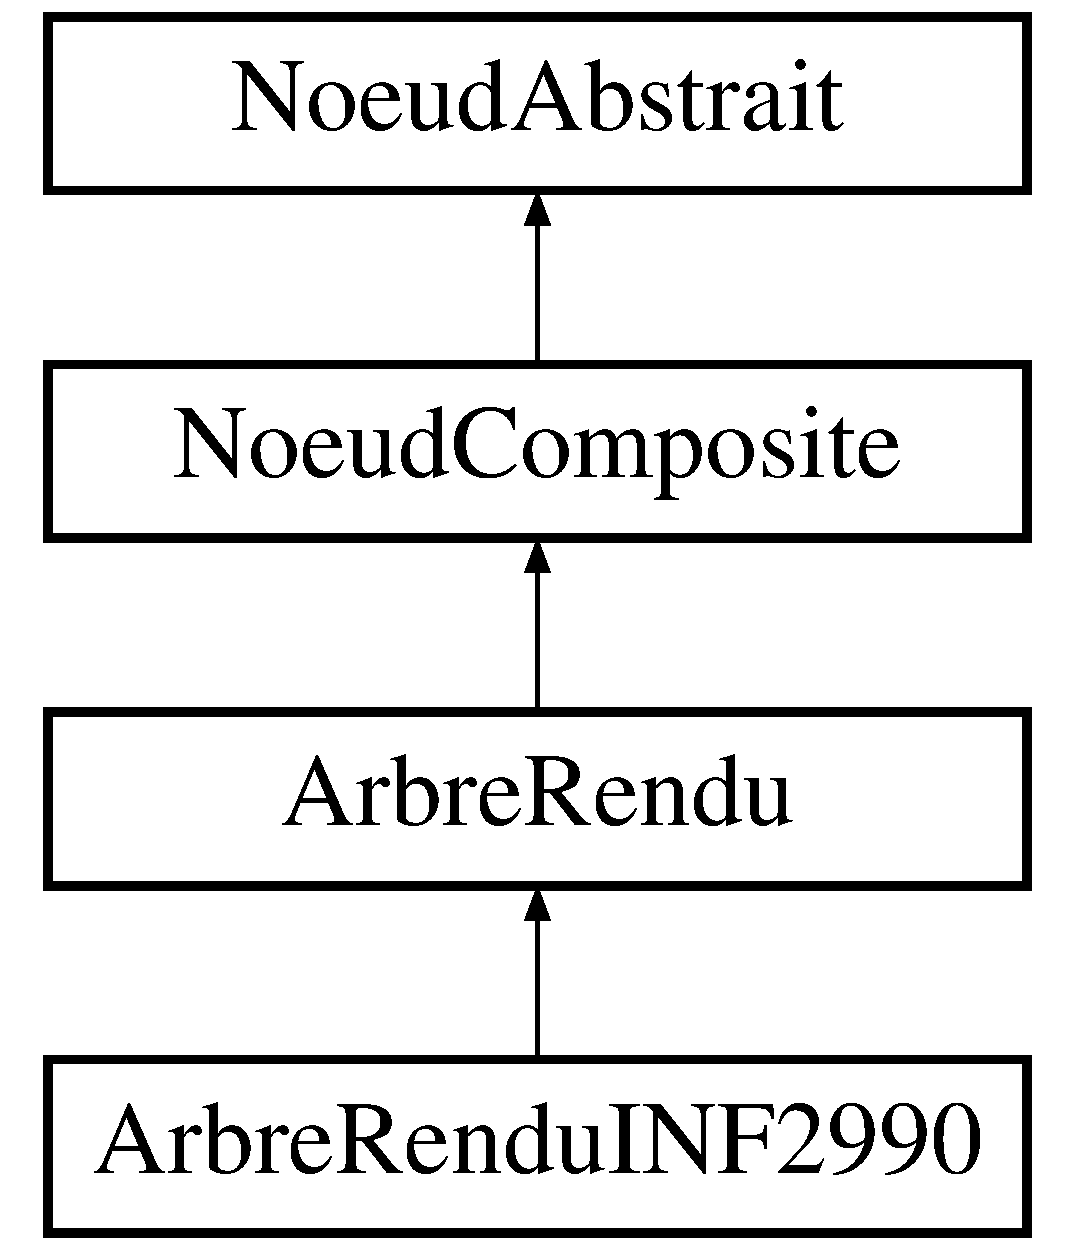
\includegraphics[height=4.000000cm]{class_arbre_rendu}
\end{center}
\end{figure}
\subsection*{Public Member Functions}
\begin{DoxyCompactItemize}
\item 
\hyperlink{group__inf2990_gaef1e98a66c4f1d3b468c786edee45ae6}{Arbre\+Rendu} ()
\begin{DoxyCompactList}\small\item\em Constructeur par d�faut. \end{DoxyCompactList}\item 
virtual \hyperlink{group__inf2990_gadb462923759da0ff632dad097b7bfdab}{$\sim$\+Arbre\+Rendu} ()
\begin{DoxyCompactList}\small\item\em Destructeur. \end{DoxyCompactList}\item 
void \hyperlink{group__inf2990_ga296a744837fb7b779fadf2e8c62e6577}{ajouter\+Usine} (const std\+::string \&type, const \hyperlink{class_usine_abstraite}{Usine\+Abstraite} $\ast$usine)
\begin{DoxyCompactList}\small\item\em Ajoute une usine associ�e � un type de noeud. \end{DoxyCompactList}\item 
\hyperlink{class_noeud_abstrait}{Noeud\+Abstrait} $\ast$ \hyperlink{group__inf2990_gaa3e9d1f8092f0c5f03b07f4eb3768259}{creer\+Noeud} (const std\+::string \&type\+Nouveau\+Noeud) const
\begin{DoxyCompactList}\small\item\em Cr�e un nouveau noeud. \end{DoxyCompactList}\item 
\hyperlink{class_noeud_abstrait}{Noeud\+Abstrait} $\ast$ {\bfseries creer\+Noeud} (const std\+::string \&type\+Nouveau\+Noeud, tinyxml2\+::\+X\+M\+L\+Node $\ast$node) const
\item 
\hyperlink{class_noeud_abstrait}{Noeud\+Abstrait} $\ast$ \hyperlink{group__inf2990_gac10e5f0623af502d67f72aef764206a3}{ajouter\+Nouveau\+Noeud} (const std\+::string \&nom\+Parent, const std\+::string \&type\+Nouveau\+Noeud)
\begin{DoxyCompactList}\small\item\em Cr�e et ajoute un nouveau noeud � l\textquotesingle{}arbre. \end{DoxyCompactList}\end{DoxyCompactItemize}
\subsection*{Static Public Member Functions}
\begin{DoxyCompactItemize}
\item 
static unsigned int \hyperlink{group__inf2990_gacf0e53d52040b07cd6550fda79867bd5}{calculer\+Profondeur\+Maximale} ()
\begin{DoxyCompactList}\small\item\em Calcule la profondeur maximale possible pour l\textquotesingle{}arbre de rendu. \end{DoxyCompactList}\end{DoxyCompactItemize}
\subsection*{Additional Inherited Members}


\subsection{Detailed Description}
Classe d\textquotesingle{}arbre de rendu qui contient la racine de l\textquotesingle{}arbre de rendu avec les usines qui permettent d\textquotesingle{}ajouter des noeuds � cet arbre. 

La profondeur de cet arbre est limit�e par la taille de la pile des matrices et la taille de la pile des noms pour la s�lection Open\+GL, �tant donn� que chaque niveau de l\textquotesingle{}arbre effectue un \char`\"{}push\char`\"{} sur chacune de ces piles lors du rendu. L\textquotesingle{}arbre ne v�rifie pas que la profondeur reste sous la limite, mais il offre des fonctions permettant de le v�rifier ais�ment.

\begin{DoxyAuthor}{Author}
Martin Bisson 
\end{DoxyAuthor}
\begin{DoxyDate}{Date}
2007-\/01-\/28 
\end{DoxyDate}


The documentation for this class was generated from the following files\+:\begin{DoxyCompactItemize}
\item 
Sources/\+D\+L\+L/\+Arbre/\hyperlink{_arbre_rendu_8h}{Arbre\+Rendu.\+h}\item 
Sources/\+D\+L\+L/\+Arbre/\hyperlink{_arbre_rendu_8cpp}{Arbre\+Rendu.\+cpp}\end{DoxyCompactItemize}

\hypertarget{class_arbre_rendu_i_n_f2990}{}\section{Arbre\+Rendu\+I\+N\+F2990 Class Reference}
\label{class_arbre_rendu_i_n_f2990}\index{Arbre\+Rendu\+I\+N\+F2990@{Arbre\+Rendu\+I\+N\+F2990}}


Classe qui représente l\textquotesingle{}arbre de rendu spécifique au projet de I\+N\+F2990.  




{\ttfamily \#include $<$Arbre\+Rendu\+I\+N\+F2990.\+h$>$}

Inheritance diagram for Arbre\+Rendu\+I\+N\+F2990\+:\begin{figure}[H]
\begin{center}
\leavevmode
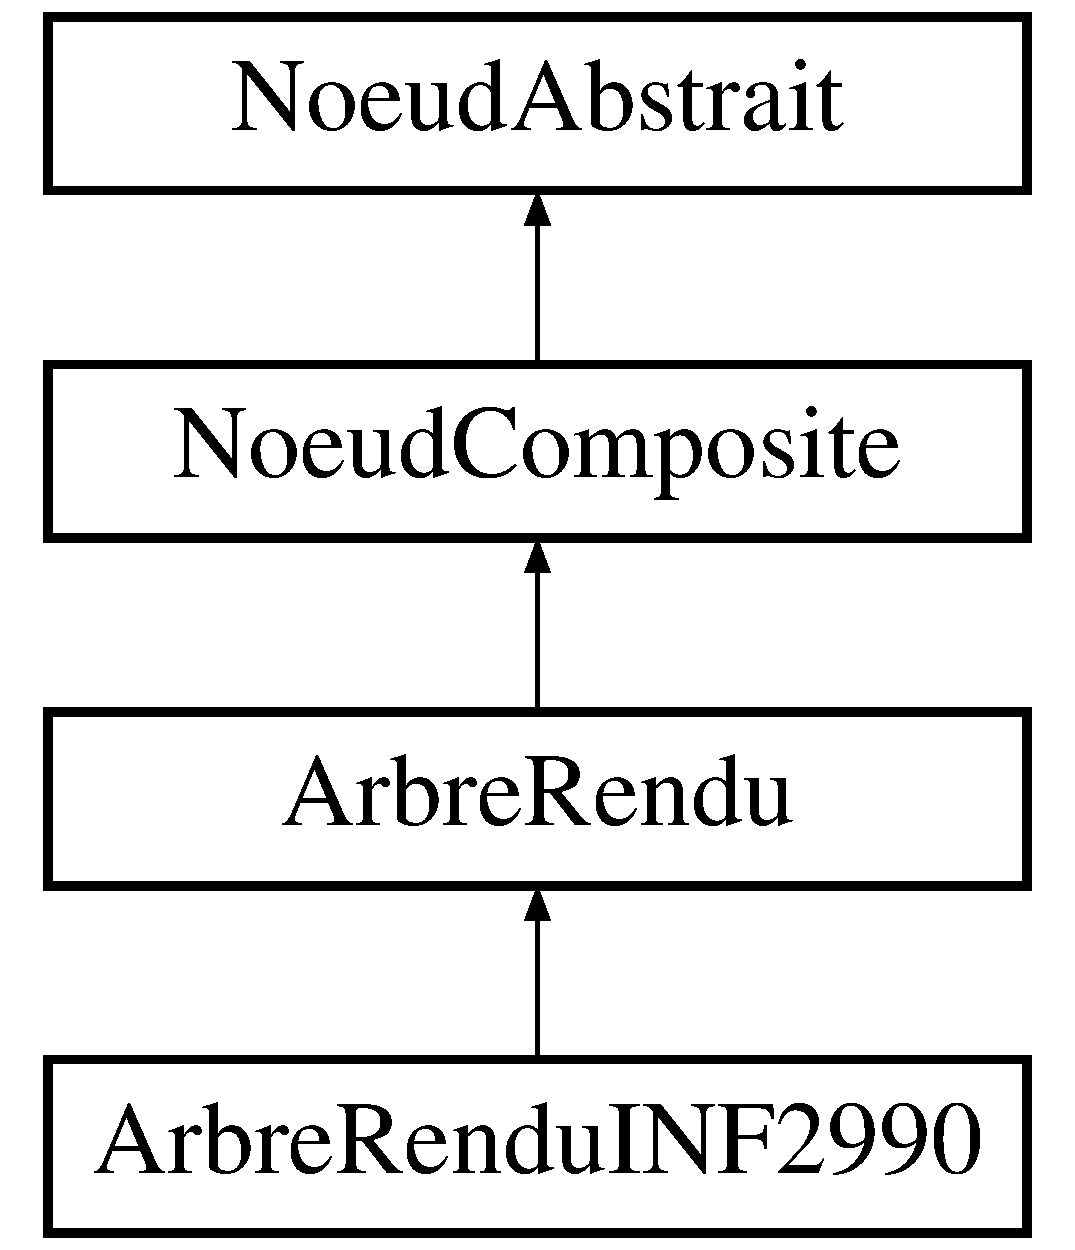
\includegraphics[height=4.000000cm]{class_arbre_rendu_i_n_f2990}
\end{center}
\end{figure}
\subsection*{Public Member Functions}
\begin{DoxyCompactItemize}
\item 
\hyperlink{group__inf2990_ga67528b7fa54e8ef8f96ef2e0bad06d2d}{Arbre\+Rendu\+I\+N\+F2990} ()
\begin{DoxyCompactList}\small\item\em Constructeur par défaut. \end{DoxyCompactList}\item 
virtual \hyperlink{group__inf2990_gaa67526b2fd719f6bcef7a4547bd25c7b}{$\sim$\+Arbre\+Rendu\+I\+N\+F2990} ()
\begin{DoxyCompactList}\small\item\em Destructeur. \end{DoxyCompactList}\item 
void \hyperlink{group__inf2990_ga678d89e1f12ae16ee7dcf6de3db637a3}{initialiser} ()
\begin{DoxyCompactList}\small\item\em Initialise l\textquotesingle{}arbre de rendu à son état initial. \end{DoxyCompactList}\item 
void \hyperlink{group__inf2990_gadfed85438e3f27c913fbe5924e378899}{initialiser\+Partie\+Avec\+Virtuel} ()
\item 
void \hyperlink{group__inf2990_gada983d8cac525061d285dd9ab2a19af8}{initialiser\+Partie\+Avec\+Humain} ()
\item 
int \hyperlink{group__inf2990_ga519bc7e5846e15f457e966d5bbfebf5d}{ajouter\+Nouveau\+Element} (const std\+::string \&nom\+Objet, glm\+::dvec3 positionR)
\item 
int \hyperlink{group__inf2990_ga4f71fa693acb730e4685e2a365d2fd28}{ajouter\+Nouveau\+Portail} (const std\+::string \&nom\+Objet, glm\+::dvec3 positionR)
\item 
\hypertarget{class_arbre_rendu_i_n_f2990_a00fc30fb9a84c745a7a73007e66fce74}{}\label{class_arbre_rendu_i_n_f2990_a00fc30fb9a84c745a7a73007e66fce74} 
void {\bfseries modifier\+Prochain\+Id} (int id)
\item 
\hypertarget{class_arbre_rendu_i_n_f2990_aa9fa6c79c277ea85540bb8e80e7cbac9}{}\label{class_arbre_rendu_i_n_f2990_aa9fa6c79c277ea85540bb8e80e7cbac9} 
int {\bfseries obtenir\+Prochain\+Id} ()
\item 
void \hyperlink{group__inf2990_ga85acac933bea59f80e07860bdef6bece}{marquer\+Selection} (int identifiant, bool en\+Inverse)
\item 
void \hyperlink{group__inf2990_gabc92694f019a765164bfd33619b4cc85}{assigner\+Zone\+Jeux} (\hyperlink{class_noeud_abstrait}{Noeud\+Abstrait} $\ast$zone)
\end{DoxyCompactItemize}
\subsection*{Static Public Attributes}
\begin{DoxyCompactItemize}
\item 
static const std\+::string \hyperlink{group__inf2990_ga1035430c1c08b95d17f891ae89b33b80}{N\+O\+M\+\_\+\+A\+R\+A\+I\+G\+N\+EE} \{ \char`\"{}araignee\char`\"{} \}
\begin{DoxyCompactList}\small\item\em La chaîne représentant le type des araignées. \end{DoxyCompactList}\item 
static const std\+::string \hyperlink{group__inf2990_gae849656178f4dad34106f525bf37341a}{N\+O\+M\+\_\+\+C\+O\+N\+E\+C\+U\+BE} \{ \char`\"{}conecube\char`\"{} \}
\begin{DoxyCompactList}\small\item\em La chaîne représentant le type des cones-\/cubes. \end{DoxyCompactList}\item 
static const std\+::string \hyperlink{group__inf2990_ga89e651c1a28481ce70f473bd15555114}{N\+O\+M\+\_\+\+T\+A\+B\+LE} \{ \char`\"{}table\char`\"{} \}
\begin{DoxyCompactList}\small\item\em La chaîne représentant le type des table. \end{DoxyCompactList}\item 
static const std\+::string \hyperlink{group__inf2990_ga2ebc17f2d21cd4e66216a7d2c374493e}{N\+O\+M\+\_\+\+R\+O\+N\+D\+E\+L\+LE} \{ \char`\"{}rondelle\char`\"{} \}
\begin{DoxyCompactList}\small\item\em La chaîne représentant le type des rondelle. \end{DoxyCompactList}\item 
static const std\+::string \hyperlink{group__inf2990_ga0c6b49184808c14c52d8e4a2ee00a00e}{N\+O\+M\+\_\+\+M\+A\+I\+L\+L\+E\+T\+\_\+1} \{ \char`\"{}maillet\char`\"{} \}
\begin{DoxyCompactList}\small\item\em La chaîne représentant le type des maillet. \end{DoxyCompactList}\item 
static const std\+::string {\bfseries N\+O\+M\+\_\+\+M\+A\+I\+L\+L\+E\+T\+\_\+2} \{ \char`\"{}maillet2\char`\"{} \}
\item 
static const std\+::string {\bfseries N\+O\+M\+\_\+\+M\+A\+I\+L\+L\+E\+T\+\_\+V} \{ \char`\"{}mailletV\char`\"{} \}
\item 
static const std\+::string {\bfseries N\+O\+M\+\_\+\+C\+E\+R\+C\+LE} \{ \char`\"{}cercle\char`\"{} \}
\item 
static const std\+::string \hyperlink{group__inf2990_gafd57ee426cc672e15633e991ae1af778}{N\+O\+M\+\_\+\+B\+O\+N\+US} \{ \char`\"{}bonus\char`\"{} \}
\begin{DoxyCompactList}\small\item\em La chaîne représentant le type des bonus. \end{DoxyCompactList}\item 
static const std\+::string {\bfseries N\+O\+M\+\_\+\+P\+O\+R\+T\+A\+IL} \{ \char`\"{}portail\char`\"{} \}
\item 
static const std\+::string {\bfseries N\+O\+M\+\_\+\+M\+U\+R\+ET} \{ \char`\"{}muret\char`\"{} \}
\end{DoxyCompactItemize}
\subsection*{Additional Inherited Members}


\subsection{Detailed Description}
Classe qui représente l\textquotesingle{}arbre de rendu spécifique au projet de I\+N\+F2990. 

Cette classe s\textquotesingle{}occupe de configurer les usines des noeuds qui seront utilisés par le projet.

\begin{DoxyAuthor}{Author}
Martin Bisson 
\end{DoxyAuthor}
\begin{DoxyDate}{Date}
2007-\/03-\/23 
\end{DoxyDate}


The documentation for this class was generated from the following files\+:\begin{DoxyCompactItemize}
\item 
Sources/\+D\+L\+L/\+Arbre/\hyperlink{_arbre_rendu_i_n_f2990_8h}{Arbre\+Rendu\+I\+N\+F2990.\+h}\item 
Sources/\+D\+L\+L/\+Arbre/\hyperlink{_arbre_rendu_i_n_f2990_8cpp}{Arbre\+Rendu\+I\+N\+F2990.\+cpp}\end{DoxyCompactItemize}

\hypertarget{class_interface_graphique_1_1_arbre_tournoi}{}\section{Interface\+Graphique.\+Arbre\+Tournoi Class Reference}
\label{class_interface_graphique_1_1_arbre_tournoi}\index{Interface\+Graphique.\+Arbre\+Tournoi@{Interface\+Graphique.\+Arbre\+Tournoi}}
Inheritance diagram for Interface\+Graphique.\+Arbre\+Tournoi\+:\begin{figure}[H]
\begin{center}
\leavevmode
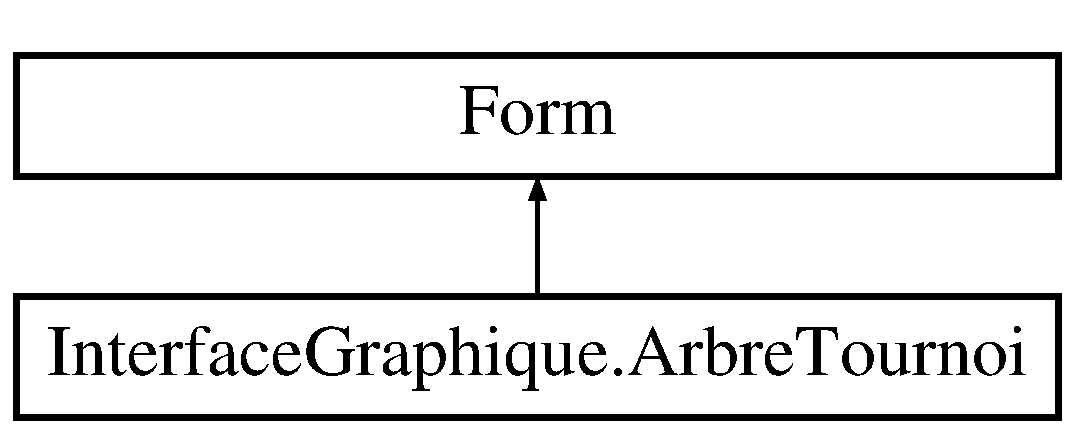
\includegraphics[height=2.000000cm]{class_interface_graphique_1_1_arbre_tournoi}
\end{center}
\end{figure}
\subsection*{Public Member Functions}
\begin{DoxyCompactItemize}
\item 
void {\bfseries mise\+A\+Jour\+Arbre} (bool joueur1\+Passe, bool joueur3\+Passe, bool vainqueur1\+Passe, bool actualiser1, bool actualiser2, bool actualiser3)
\item 
void {\bfseries initialisation\+Noms\+Joueur} (string nom1, string nom2, string nom3, string nom4)
\end{DoxyCompactItemize}
\subsection*{Protected Member Functions}
\begin{DoxyCompactItemize}
\item 
override void \hyperlink{class_interface_graphique_1_1_arbre_tournoi_a02a9179ff4e8e7226530694ed9078e66}{Dispose} (bool disposing)
\begin{DoxyCompactList}\small\item\em Clean up any resources being used. \end{DoxyCompactList}\end{DoxyCompactItemize}


\subsection{Member Function Documentation}
\hypertarget{class_interface_graphique_1_1_arbre_tournoi_a02a9179ff4e8e7226530694ed9078e66}{}\label{class_interface_graphique_1_1_arbre_tournoi_a02a9179ff4e8e7226530694ed9078e66} 
\index{Interface\+Graphique\+::\+Arbre\+Tournoi@{Interface\+Graphique\+::\+Arbre\+Tournoi}!Dispose@{Dispose}}
\index{Dispose@{Dispose}!Interface\+Graphique\+::\+Arbre\+Tournoi@{Interface\+Graphique\+::\+Arbre\+Tournoi}}
\subsubsection{\texorpdfstring{Dispose()}{Dispose()}}
{\footnotesize\ttfamily override void Interface\+Graphique.\+Arbre\+Tournoi.\+Dispose (\begin{DoxyParamCaption}\item[{bool}]{disposing }\end{DoxyParamCaption})\hspace{0.3cm}{\ttfamily [inline]}, {\ttfamily [protected]}}



Clean up any resources being used. 


\begin{DoxyParams}{Parameters}
{\em disposing} & true if managed resources should be disposed; otherwise, false.\\
\hline
\end{DoxyParams}


The documentation for this class was generated from the following files\+:\begin{DoxyCompactItemize}
\item 
C\+:/\+Users/\+Steven/\+Documents/\+Poly/\+I\+N\+F2990/inf2990-\/06/\+Cadriciel\+\_\+2016-\/3\+\_\+\+Etudiants/\+Cadriciel/\+Sources/\+Interface\+Graphique/Arbre\+Tournoi.\+cs\item 
C\+:/\+Users/\+Steven/\+Documents/\+Poly/\+I\+N\+F2990/inf2990-\/06/\+Cadriciel\+\_\+2016-\/3\+\_\+\+Etudiants/\+Cadriciel/\+Sources/\+Interface\+Graphique/Arbre\+Tournoi.\+Designer.\+cs\end{DoxyCompactItemize}

\hypertarget{class_banc_tests}{}\section{Banc\+Tests Class Reference}
\label{class_banc_tests}\index{Banc\+Tests@{Banc\+Tests}}


Banc de tests qui permet d\textquotesingle{}ex�cuter tous les tests unitaires. C\textquotesingle{}est une classe singleton.  




{\ttfamily \#include $<$Banc\+Tests.\+h$>$}

Inheritance diagram for Banc\+Tests\+:\begin{figure}[H]
\begin{center}
\leavevmode
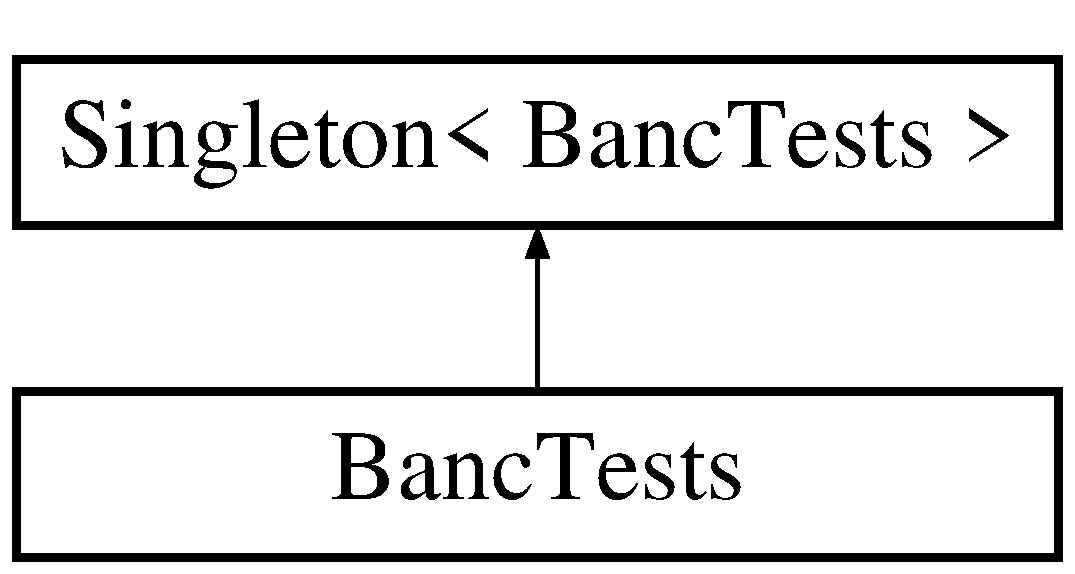
\includegraphics[height=2.000000cm]{class_banc_tests}
\end{center}
\end{figure}
\subsection*{Public Member Functions}
\begin{DoxyCompactItemize}
\item 
bool \hyperlink{group__inf2990_gab5d7fbfe7e3fbe00aa187caa10b1c506}{executer} ()
\begin{DoxyCompactList}\small\item\em Ex�cuter tous les tests unitaires. \end{DoxyCompactList}\end{DoxyCompactItemize}


\subsection{Detailed Description}
Banc de tests qui permet d\textquotesingle{}ex�cuter tous les tests unitaires. C\textquotesingle{}est une classe singleton. 

\begin{DoxyAuthor}{Author}
Julien Gascon-\/\+Samson 
\end{DoxyAuthor}
\begin{DoxyDate}{Date}
2011-\/07-\/16 
\end{DoxyDate}


The documentation for this class was generated from the following files\+:\begin{DoxyCompactItemize}
\item 
Sources/\+D\+L\+L/\+Tests/\hyperlink{_banc_tests_8h}{Banc\+Tests.\+h}\item 
Sources/\+D\+L\+L/\+Tests/\hyperlink{_banc_tests_8cpp}{Banc\+Tests.\+cpp}\end{DoxyCompactItemize}

\hypertarget{class_config_scene}{}\section{Config\+Scene Class Reference}
\label{class_config_scene}\index{Config\+Scene@{Config\+Scene}}


Les variables de configuration de la classe C\+Scene. C\textquotesingle{}est une classe singleton.  




{\ttfamily \#include $<$Config\+Scene.\+h$>$}

Inheritance diagram for Config\+Scene\+:\begin{figure}[H]
\begin{center}
\leavevmode
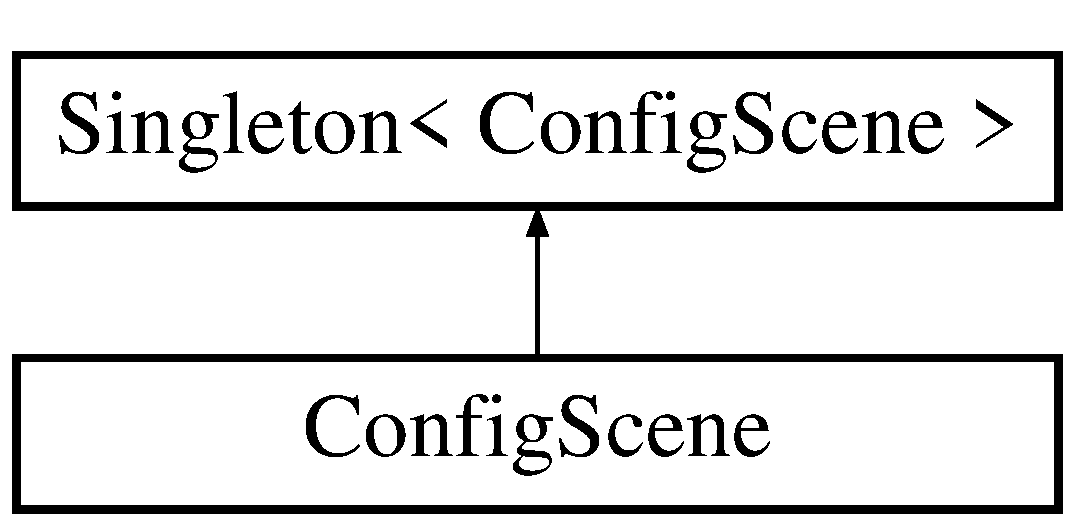
\includegraphics[height=2.000000cm]{class_config_scene}
\end{center}
\end{figure}
\subsection*{Public Member Functions}
\begin{DoxyCompactItemize}
\item 
void \hyperlink{group__inf2990_ga8eb1610fff0a4771d14d3770a0a18ddc}{creer\+D\+OM} (tinyxml2\+::\+X\+M\+L\+Document \&document) const
\begin{DoxyCompactList}\small\item\em Cr�er le D\+OM avec les valeurs. \end{DoxyCompactList}\item 
void \hyperlink{group__inf2990_gaeacd60be947ce76a1302f6bbb40c90b1}{lire\+D\+OM} (tinyxml2\+::\+X\+M\+L\+Document const \&document)
\begin{DoxyCompactList}\small\item\em Lire les valeurs du D\+OM. \end{DoxyCompactList}\end{DoxyCompactItemize}
\subsection*{Static Public Attributes}
\begin{DoxyCompactItemize}
\item 
static int \hyperlink{group__inf2990_gadb487b450a0314a5d1f75cf31ce502eb}{C\+A\+L\+C\+U\+L\+S\+\_\+\+P\+A\+R\+\_\+\+I\+M\+A\+GE} \{ 50 \}
\begin{DoxyCompactList}\small\item\em Nombre de calculs par image. \end{DoxyCompactList}\end{DoxyCompactItemize}


\subsection{Detailed Description}
Les variables de configuration de la classe C\+Scene. C\textquotesingle{}est une classe singleton. 

\begin{DoxyAuthor}{Author}
Jean-\/\+Fran�ois P�russe 
\end{DoxyAuthor}
\begin{DoxyDate}{Date}
2007-\/01-\/10 
\end{DoxyDate}


The documentation for this class was generated from the following files\+:\begin{DoxyCompactItemize}
\item 
C\+:/\+Users/\+Steven/\+Documents/\+Poly/\+I\+N\+F2990/inf2990-\/06/\+Cadriciel\+\_\+2016-\/3\+\_\+\+Etudiants/\+Cadriciel/\+Sources/\+D\+L\+L/\+Configuration/\hyperlink{_config_scene_8h}{Config\+Scene.\+h}\item 
C\+:/\+Users/\+Steven/\+Documents/\+Poly/\+I\+N\+F2990/inf2990-\/06/\+Cadriciel\+\_\+2016-\/3\+\_\+\+Etudiants/\+Cadriciel/\+Sources/\+D\+L\+L/\+Configuration/\hyperlink{_config_scene_8cpp}{Config\+Scene.\+cpp}\end{DoxyCompactItemize}

\hypertarget{class_config_scene_test}{}\section{Config\+Scene\+Test Class Reference}
\label{class_config_scene_test}\index{Config\+Scene\+Test@{Config\+Scene\+Test}}


Classe de test cppunit pour tester le bon fonctionnement des m�thodes de la classe \hyperlink{class_config_scene}{Config\+Scene}.  




{\ttfamily \#include $<$Config\+Scene\+Test.\+h$>$}

Inheritance diagram for Config\+Scene\+Test\+:\begin{figure}[H]
\begin{center}
\leavevmode
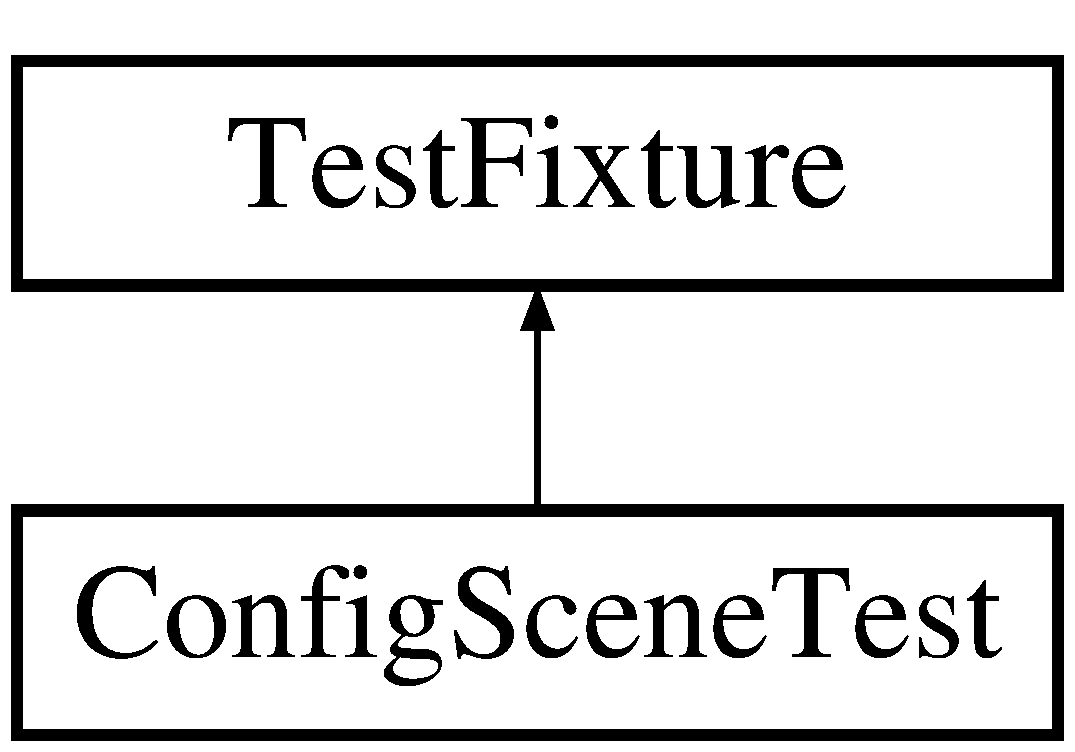
\includegraphics[height=2.000000cm]{class_config_scene_test}
\end{center}
\end{figure}
\subsection*{Public Member Functions}
\begin{DoxyCompactItemize}
\item 
void \hyperlink{group__inf2990_ga707d7400843047e67b736ab79bafb5a0}{set\+Up} ()
\begin{DoxyCompactList}\small\item\em Traitement � effectuer pour initialiser cette suite de tests. \end{DoxyCompactList}\item 
void \hyperlink{group__inf2990_ga889ed3891c3e55280cabb982953906d9}{tear\+Down} ()
\begin{DoxyCompactList}\small\item\em Traitement � effectuer pour \textquotesingle{}finaliser\textquotesingle{} cette suite de tests. \end{DoxyCompactList}\item 
void \hyperlink{group__inf2990_ga0f09d52bc30d87f18b0341e1052efb74}{test\+Sauvegarde\+Chargement} ()
\begin{DoxyCompactList}\small\item\em Cas de test\+: sauvegarde et chargement X\+ML de la configuration. \end{DoxyCompactList}\end{DoxyCompactItemize}


\subsection{Detailed Description}
Classe de test cppunit pour tester le bon fonctionnement des m�thodes de la classe \hyperlink{class_config_scene}{Config\+Scene}. 

\begin{DoxyAuthor}{Author}
Julien Gascon-\/\+Samson 
\end{DoxyAuthor}
\begin{DoxyDate}{Date}
2011-\/07-\/16 
\end{DoxyDate}


The documentation for this class was generated from the following files\+:\begin{DoxyCompactItemize}
\item 
C\+:/\+Users/\+Steven/\+Documents/\+Poly/\+I\+N\+F2990/inf2990-\/06/\+Cadriciel\+\_\+2016-\/3\+\_\+\+Etudiants/\+Cadriciel/\+Sources/\+D\+L\+L/\+Tests/\hyperlink{_config_scene_test_8h}{Config\+Scene\+Test.\+h}\item 
C\+:/\+Users/\+Steven/\+Documents/\+Poly/\+I\+N\+F2990/inf2990-\/06/\+Cadriciel\+\_\+2016-\/3\+\_\+\+Etudiants/\+Cadriciel/\+Sources/\+D\+L\+L/\+Tests/\hyperlink{_config_scene_test_8cpp}{Config\+Scene\+Test.\+cpp}\end{DoxyCompactItemize}

\hypertarget{class_interface_graphique_1_1_configuration}{}\section{Interface\+Graphique.\+Configuration Class Reference}
\label{class_interface_graphique_1_1_configuration}\index{Interface\+Graphique.\+Configuration@{Interface\+Graphique.\+Configuration}}
Inheritance diagram for Interface\+Graphique.\+Configuration\+:\begin{figure}[H]
\begin{center}
\leavevmode
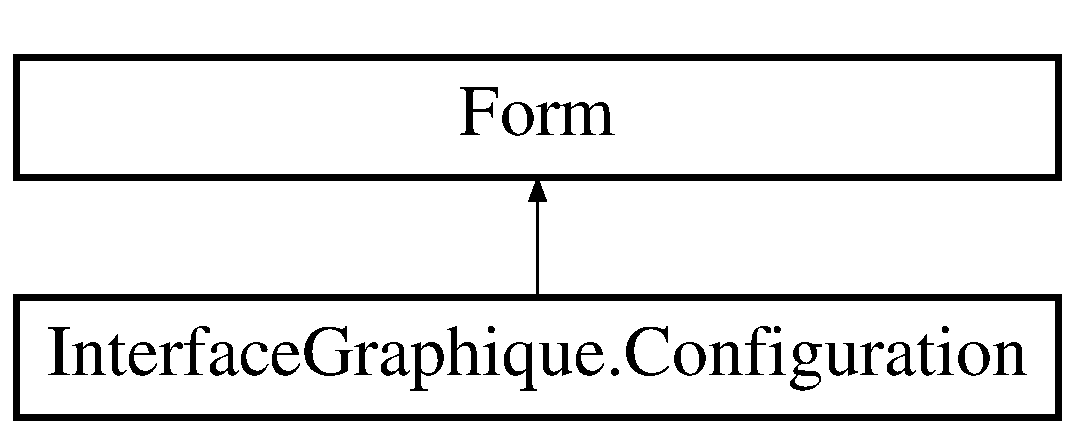
\includegraphics[height=2.000000cm]{class_interface_graphique_1_1_configuration}
\end{center}
\end{figure}
\subsection*{Public Member Functions}
\begin{DoxyCompactItemize}
\item 
\hyperlink{group__inf2990_gadb0bf51b9f3e30cfed923c7d9d950493}{Configuration} ()
\end{DoxyCompactItemize}
\subsection*{Static Public Attributes}
\begin{DoxyCompactItemize}
\item 
static bool {\bfseries changer\+Touche\+Haut} = false
\item 
static bool {\bfseries changer\+Touche\+Bas} = false
\item 
static bool {\bfseries changer\+Touche\+Gauche} = false
\item 
static bool {\bfseries changer\+Touche\+Droite} = false
\item 
static List$<$ \hyperlink{struct_interface_graphique_1_1_profil}{Profil} $>$ {\bfseries liste\+Profils} = new List$<$\hyperlink{struct_interface_graphique_1_1_profil}{Profil}$>$()
\item 
static bool {\bfseries peut\+Afficher\+Debogage}
\item 
static bool {\bfseries peut\+Afficher\+Collision}
\item 
static bool {\bfseries peut\+Afficher\+Vitesse\+Rondelle}
\item 
static bool {\bfseries peut\+Afficher\+Eclairage}
\item 
static bool {\bfseries peut\+Afficher\+Attraction\+Portail}
\item 
static int {\bfseries nb\+Buts}
\item 
static string {\bfseries haut}
\item 
static string {\bfseries bas}
\item 
static string {\bfseries gauche}
\item 
static string {\bfseries droite}
\item 
static bool {\bfseries est\+Virtuel}
\end{DoxyCompactItemize}
\subsection*{Protected Member Functions}
\begin{DoxyCompactItemize}
\item 
override bool \hyperlink{group__inf2990_ga1acc9513c830f0ef53c3fb0ded70bf44}{Process\+Cmd\+Key} (ref Message msg, Keys key\+Data)
\begin{DoxyCompactList}\small\item\em Pour modifier les touches selon le bouton de l\textquotesingle{}usager. \end{DoxyCompactList}\item 
override void \hyperlink{class_interface_graphique_1_1_configuration_a0200b084946b5710be7d94f9e8b0385c}{Dispose} (bool disposing)
\begin{DoxyCompactList}\small\item\em Clean up any resources being used. \end{DoxyCompactList}\end{DoxyCompactItemize}


\subsection{Member Function Documentation}
\hypertarget{class_interface_graphique_1_1_configuration_a0200b084946b5710be7d94f9e8b0385c}{}\label{class_interface_graphique_1_1_configuration_a0200b084946b5710be7d94f9e8b0385c} 
\index{Interface\+Graphique\+::\+Configuration@{Interface\+Graphique\+::\+Configuration}!Dispose@{Dispose}}
\index{Dispose@{Dispose}!Interface\+Graphique\+::\+Configuration@{Interface\+Graphique\+::\+Configuration}}
\subsubsection{\texorpdfstring{Dispose()}{Dispose()}}
{\footnotesize\ttfamily override void Interface\+Graphique.\+Configuration.\+Dispose (\begin{DoxyParamCaption}\item[{bool}]{disposing }\end{DoxyParamCaption})\hspace{0.3cm}{\ttfamily [inline]}, {\ttfamily [protected]}}



Clean up any resources being used. 


\begin{DoxyParams}{Parameters}
{\em disposing} & true if managed resources should be disposed; otherwise, false.\\
\hline
\end{DoxyParams}


The documentation for this class was generated from the following files\+:\begin{DoxyCompactItemize}
\item 
Sources/\+Interface\+Graphique/\hyperlink{_configuration_8cs}{Configuration.\+cs}\item 
Sources/\+Interface\+Graphique/Configuration.\+Designer.\+cs\end{DoxyCompactItemize}

\hypertarget{class_interface_graphique_1_1_configuration_partie_rapide}{}\section{Interface\+Graphique.\+Configuration\+Partie\+Rapide Class Reference}
\label{class_interface_graphique_1_1_configuration_partie_rapide}\index{Interface\+Graphique.\+Configuration\+Partie\+Rapide@{Interface\+Graphique.\+Configuration\+Partie\+Rapide}}
Inheritance diagram for Interface\+Graphique.\+Configuration\+Partie\+Rapide\+:\begin{figure}[H]
\begin{center}
\leavevmode
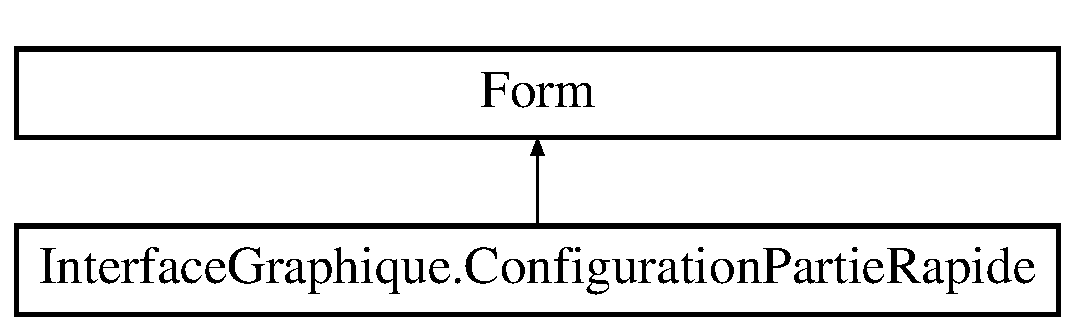
\includegraphics[height=2.000000cm]{class_interface_graphique_1_1_configuration_partie_rapide}
\end{center}
\end{figure}
\subsection*{Protected Member Functions}
\begin{DoxyCompactItemize}
\item 
override void \hyperlink{class_interface_graphique_1_1_configuration_partie_rapide_a783af7dcd620d9b43374b22218a878ea}{Dispose} (bool disposing)
\begin{DoxyCompactList}\small\item\em Clean up any resources being used. \end{DoxyCompactList}\end{DoxyCompactItemize}


\subsection{Member Function Documentation}
\hypertarget{class_interface_graphique_1_1_configuration_partie_rapide_a783af7dcd620d9b43374b22218a878ea}{}\label{class_interface_graphique_1_1_configuration_partie_rapide_a783af7dcd620d9b43374b22218a878ea} 
\index{Interface\+Graphique\+::\+Configuration\+Partie\+Rapide@{Interface\+Graphique\+::\+Configuration\+Partie\+Rapide}!Dispose@{Dispose}}
\index{Dispose@{Dispose}!Interface\+Graphique\+::\+Configuration\+Partie\+Rapide@{Interface\+Graphique\+::\+Configuration\+Partie\+Rapide}}
\subsubsection{\texorpdfstring{Dispose()}{Dispose()}}
{\footnotesize\ttfamily override void Interface\+Graphique.\+Configuration\+Partie\+Rapide.\+Dispose (\begin{DoxyParamCaption}\item[{bool}]{disposing }\end{DoxyParamCaption})\hspace{0.3cm}{\ttfamily [inline]}, {\ttfamily [protected]}}



Clean up any resources being used. 


\begin{DoxyParams}{Parameters}
{\em disposing} & true if managed resources should be disposed; otherwise, false.\\
\hline
\end{DoxyParams}


The documentation for this class was generated from the following files\+:\begin{DoxyCompactItemize}
\item 
Sources/\+Interface\+Graphique/\hyperlink{_configuration_partie_rapide_8cs}{Configuration\+Partie\+Rapide.\+cs}\item 
Sources/\+Interface\+Graphique/Configuration\+Partie\+Rapide.\+Designer.\+cs\end{DoxyCompactItemize}

\hypertarget{class_interface_graphique_1_1_configuration_tournoi}{}\section{Interface\+Graphique.\+Configuration\+Tournoi Class Reference}
\label{class_interface_graphique_1_1_configuration_tournoi}\index{Interface\+Graphique.\+Configuration\+Tournoi@{Interface\+Graphique.\+Configuration\+Tournoi}}
Inheritance diagram for Interface\+Graphique.\+Configuration\+Tournoi\+:\begin{figure}[H]
\begin{center}
\leavevmode
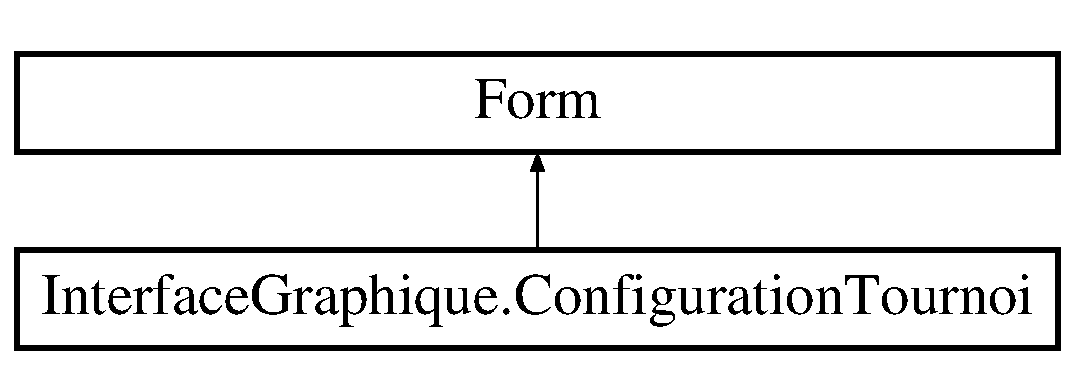
\includegraphics[height=2.000000cm]{class_interface_graphique_1_1_configuration_tournoi}
\end{center}
\end{figure}
\subsection*{Static Public Attributes}
\begin{DoxyCompactItemize}
\item 
static bool {\bfseries joueur1\+Est\+Virtuel} = false
\item 
static bool {\bfseries joueur2\+Est\+Virtuel} = false
\item 
static bool {\bfseries joueur3\+Est\+Virtuel} = false
\item 
static bool {\bfseries joueur4\+Est\+Virtuel} = false
\item 
static string {\bfseries joueur1} = \char`\"{}joueur1\char`\"{}
\item 
static string {\bfseries joueur2} = \char`\"{}joueur2\char`\"{}
\item 
static string {\bfseries joueur3} = \char`\"{}joueur3\char`\"{}
\item 
static string {\bfseries joueur4} = \char`\"{}joueur4\char`\"{}
\end{DoxyCompactItemize}
\subsection*{Protected Member Functions}
\begin{DoxyCompactItemize}
\item 
override void \hyperlink{class_interface_graphique_1_1_configuration_tournoi_ad801e75807538977aa896ae679e403ec}{Dispose} (bool disposing)
\begin{DoxyCompactList}\small\item\em Clean up any resources being used. \end{DoxyCompactList}\end{DoxyCompactItemize}


\subsection{Member Function Documentation}
\hypertarget{class_interface_graphique_1_1_configuration_tournoi_ad801e75807538977aa896ae679e403ec}{}\label{class_interface_graphique_1_1_configuration_tournoi_ad801e75807538977aa896ae679e403ec} 
\index{Interface\+Graphique\+::\+Configuration\+Tournoi@{Interface\+Graphique\+::\+Configuration\+Tournoi}!Dispose@{Dispose}}
\index{Dispose@{Dispose}!Interface\+Graphique\+::\+Configuration\+Tournoi@{Interface\+Graphique\+::\+Configuration\+Tournoi}}
\subsubsection{\texorpdfstring{Dispose()}{Dispose()}}
{\footnotesize\ttfamily override void Interface\+Graphique.\+Configuration\+Tournoi.\+Dispose (\begin{DoxyParamCaption}\item[{bool}]{disposing }\end{DoxyParamCaption})\hspace{0.3cm}{\ttfamily [inline]}, {\ttfamily [protected]}}



Clean up any resources being used. 


\begin{DoxyParams}{Parameters}
{\em disposing} & true if managed resources should be disposed; otherwise, false.\\
\hline
\end{DoxyParams}


The documentation for this class was generated from the following files\+:\begin{DoxyCompactItemize}
\item 
Sources/\+Interface\+Graphique/\hyperlink{_configuration_tournoi_8cs}{Configuration\+Tournoi.\+cs}\item 
Sources/\+Interface\+Graphique/Configuration\+Tournoi.\+Designer.\+cs\end{DoxyCompactItemize}

\hypertarget{class_interface_graphique_1_1_etat_edition_rondelle}{}\section{Interface\+Graphique.\+Etat\+Edition\+Rondelle Class Reference}
\label{class_interface_graphique_1_1_etat_edition_rondelle}\index{Interface\+Graphique.\+Etat\+Edition\+Rondelle@{Interface\+Graphique.\+Etat\+Edition\+Rondelle}}
Inheritance diagram for Interface\+Graphique.\+Etat\+Edition\+Rondelle\+:\begin{figure}[H]
\begin{center}
\leavevmode
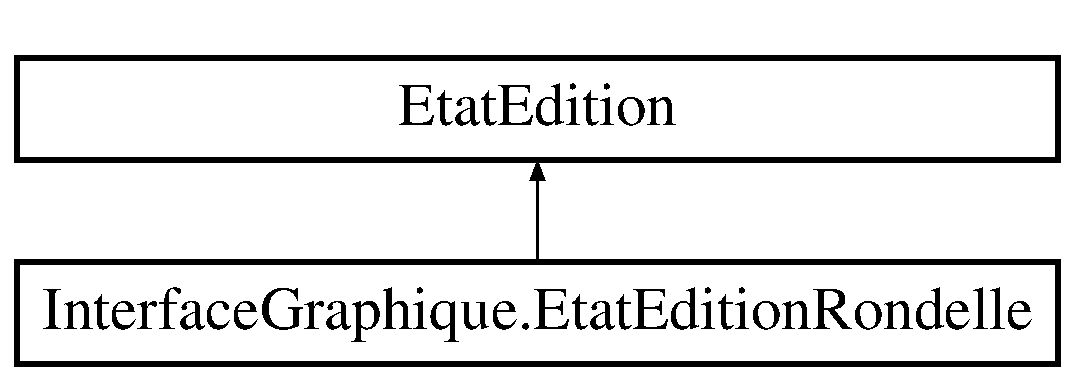
\includegraphics[height=2.000000cm]{class_interface_graphique_1_1_etat_edition_rondelle}
\end{center}
\end{figure}
\subsection*{Public Member Functions}
\begin{DoxyCompactItemize}
\item 
\hypertarget{class_interface_graphique_1_1_etat_edition_rondelle_a33e725c3e9db6f9c822bbe75ab9328c5}{}\label{class_interface_graphique_1_1_etat_edition_rondelle_a33e725c3e9db6f9c822bbe75ab9328c5} 
override void {\bfseries interpretation\+Clic} (int x, int y, Keys k)
\item 
\hypertarget{class_interface_graphique_1_1_etat_edition_rondelle_ab7559d67e73d6055184a503025ea7456}{}\label{class_interface_graphique_1_1_etat_edition_rondelle_ab7559d67e73d6055184a503025ea7456} 
override bool {\bfseries verifier\+Clic} (int x, int y)
\end{DoxyCompactItemize}


The documentation for this class was generated from the following file\+:\begin{DoxyCompactItemize}
\item 
C\+:/\+Users/\+Steven/\+Documents/\+Poly/\+I\+N\+F2990/inf2990-\/06/\+Cadriciel\+\_\+2016-\/3\+\_\+\+Etudiants/\+Cadriciel/\+Sources/\+Interface\+Graphique/Etat\+Edition\+Rondelle.\+cs\end{DoxyCompactItemize}

\hypertarget{class_facade_modele}{}\section{Facade\+Modele Class Reference}
\label{class_facade_modele}\index{Facade\+Modele@{Facade\+Modele}}


Classe qui constitue une interface (une fa�ade) sur l\textquotesingle{}ensemble du mod�le et des classes qui le composent.  




{\ttfamily \#include $<$Facade\+Modele.\+h$>$}

\subsection*{Public Member Functions}
\begin{DoxyCompactItemize}
\item 
void \hyperlink{group__inf2990_gabf12ccafbabf1049cb8327cf78699a1b}{initialiser\+Open\+GL} (H\+W\+ND h\+Wnd)
\begin{DoxyCompactList}\small\item\em Cr�e un contexte Open\+GL et initialise celui-\/ci. \end{DoxyCompactList}\item 
void \hyperlink{group__inf2990_ga4128d21c2ccdaefdb8a2ae7929bb2175}{charger\+Configuration} () const
\begin{DoxyCompactList}\small\item\em Charge la configuration � partir d\textquotesingle{}un fichier X\+ML. \end{DoxyCompactList}\item 
void \hyperlink{group__inf2990_gaa38f6ffdb4ae0b8e77e0108a57da2714}{enregistrer\+Configuration} () const
\begin{DoxyCompactList}\small\item\em Enregistre la configuration courante dans un fichier X\+ML. \end{DoxyCompactList}\item 
void \hyperlink{group__inf2990_gac7b831ce13626514e9637c4533d7c15d}{liberer\+Open\+GL} ()
\begin{DoxyCompactList}\small\item\em Lib�re le contexte Open\+GL. \end{DoxyCompactList}\item 
void \hyperlink{group__inf2990_ga0bdd801a0d7be5059c4d9ff8f55f6b62}{afficher} () const
\begin{DoxyCompactList}\small\item\em Affiche le contenu du mod�le. \end{DoxyCompactList}\item 
void \hyperlink{group__inf2990_ga8fd84489fa3f0936e6fd5a2e6d9d9439}{afficher\+Base} () const
\begin{DoxyCompactList}\small\item\em Affiche la base du contenu du mod�le. \end{DoxyCompactList}\item 
void \hyperlink{group__inf2990_ga12ab3532311b25c8f95bf116ff50c340}{initialiser\+Rectangle\+Elas} (int x, int y)
\begin{DoxyCompactList}\small\item\em initialier le rectangle elastique \end{DoxyCompactList}\item 
void \hyperlink{group__inf2990_gad62020361b7b54738ce1f043b593a899}{mettre\+A\+Jour\+Rectangle\+Elas} (int x1, int y1)
\begin{DoxyCompactList}\small\item\em mettre a jour le rectangle elastique \end{DoxyCompactList}\item 
void \hyperlink{group__inf2990_gadcc8863ea29b0f4cea87325cc910455f}{terminer\+Rectangle\+Elas} ()
\begin{DoxyCompactList}\small\item\em finalise le rectangle elastique \end{DoxyCompactList}\item 
void \hyperlink{group__inf2990_gad76f00b2335eadd3807334196490c162}{zoom\+In\+Elas} ()
\begin{DoxyCompactList}\small\item\em Zoom in grace au rectangle elestique. \end{DoxyCompactList}\item 
void \hyperlink{group__inf2990_ga0364cd87c45bb8555e5489529c9397e3}{zoom\+Out\+Elas} ()
\begin{DoxyCompactList}\small\item\em Zoom in grace au rectangle elestique. \end{DoxyCompactList}\item 
void \hyperlink{group__inf2990_gad72a7884085823a04fde536274aa3f12}{selection\+Rectangle} ()
\begin{DoxyCompactList}\small\item\em Selection avec rectangle elastique. \end{DoxyCompactList}\item 
vue\+::\+Vue $\ast$ \hyperlink{group__inf2990_gaa56cf96b7e381e0f14e2c9a55be913bf}{obtenir\+Vue} ()
\begin{DoxyCompactList}\small\item\em Retourne la vue courante. \end{DoxyCompactList}\item 
const \hyperlink{class_arbre_rendu_i_n_f2990}{Arbre\+Rendu\+I\+N\+F2990} $\ast$ \hyperlink{group__inf2990_ga381a8c1927abe900473fe663a0a9132d}{obtenir\+Arbre\+Rendu\+I\+N\+F2990} () const
\begin{DoxyCompactList}\small\item\em Retourne l\textquotesingle{}arbre de rendu. \end{DoxyCompactList}\item 
\hyperlink{class_arbre_rendu_i_n_f2990}{Arbre\+Rendu\+I\+N\+F2990} $\ast$ \hyperlink{group__inf2990_ga12d5594db6a9507b24c7e1ffcd6751af}{obtenir\+Arbre\+Rendu\+I\+N\+F2990} ()
\begin{DoxyCompactList}\small\item\em Retourne l\textquotesingle{}arbre de rendu. \end{DoxyCompactList}\item 
int \hyperlink{group__inf2990_ga9748abad7e15bbdd3e4f75910bd0ea0e}{ajouter\+Nouveau\+Element} (char $\ast$nom\+Objet, int x, int y)
\begin{DoxyCompactList}\small\item\em Permet d\textquotesingle{}ajouter un noeud sans transformation sur la scene. \end{DoxyCompactList}\item 
int {\bfseries ajouter\+Nouveau\+Portail} (char $\ast$nom\+Objet, int x, int y)
\item 
void \hyperlink{group__inf2990_ga4c2a991fe2297e44eeee0de111fb08d2}{reinitialiser} ()
\begin{DoxyCompactList}\small\item\em R�initialise la sc�ne. \end{DoxyCompactList}\item 
void \hyperlink{group__inf2990_ga24dcb4e32cf104797158b398bafbfbb7}{animer} (float temps)
\begin{DoxyCompactList}\small\item\em Anime la sc�ne. \end{DoxyCompactList}\item 
void {\bfseries redessiner} ()
\item 
void \hyperlink{group__inf2990_ga85f2afcb297fbcaeb3cb96402e440671}{determiner\+Couleur\+Pixel} (int posX, int posY, G\+Lubyte couleur\+Pixel\mbox{[}$\,$\mbox{]})
\item 
void \hyperlink{group__inf2990_ga2b89ce775f045c41e61081d6271eaf1e}{selection\+Objet} (int posX, int posY, bool selection\+Unique)
\item 
void \hyperlink{group__inf2990_gaffcf7c590a0ae08d5b018d646b6e6b9d}{mettre\+A\+Echelle} (int x, int y)
\item 
void \hyperlink{group__inf2990_gae4dafde19e9c66c81a2937af9884a987}{initialiser\+Rotation} (int pointY)
\begin{DoxyCompactList}\small\item\em Initialise la rotation en prenant le point initial de la souris. \end{DoxyCompactList}\item 
void \hyperlink{group__inf2990_gaa11820c8cd950a8aa4bab5c8a5cffae2}{initialiser\+Deplacement} (int pointX, int pointY)
\begin{DoxyCompactList}\small\item\em Initialise le deplacement en prenant le point initial de la souris. \end{DoxyCompactList}\item 
void \hyperlink{group__inf2990_ga3df43140795a4426e4408e968a21f22f}{effectuer\+Rotation} (int pointY)
\begin{DoxyCompactList}\small\item\em Effectuer la rotation sur les objets selectionnes. \end{DoxyCompactList}\item 
void \hyperlink{group__inf2990_ga3674bdc526c4046c7a53393fa0183d1c}{effectuer\+Deplacement} (float x, float y)
\begin{DoxyCompactList}\small\item\em Effectuer le deplacement des objets. \end{DoxyCompactList}\item 
double \hyperlink{group__inf2990_gad132f27b4e86f25aef4d8b9ad93fe210}{obtenir\+Friction\+Table} ()
\item 
double \hyperlink{group__inf2990_ga2f768cce7db86eba06e1e448a4efa2f2}{obtenir\+Acceleration\+Bonus} ()
\item 
double \hyperlink{group__inf2990_ga1376bb78e311e9c724cd87d454a385b6}{obtenir\+Coef\+Rebondissement} ()
\item 
int \hyperlink{group__inf2990_gae6d3005130428ead82d1dfbcab7332ca}{obtenir\+Position\+ObjetX} ()
\item 
int \hyperlink{group__inf2990_ga9cebbfb71c3263597c8f0ddfb0bf78bd}{obtenir\+Position\+ObjetY} ()
\item 
int \hyperlink{group__inf2990_gadbef9c5a1e0a2c76a0de1186763b4801}{obtenir\+Position\+ObjetZ} ()
\item 
int \hyperlink{group__inf2990_ga23433e7ffee476584b4744e788e852cd}{obtenir\+Angle\+Rotation\+Objet} ()
\item 
double \hyperlink{group__inf2990_ga57c0c4ae3a71280a05382ff4d5e12e54}{obtenir\+Facteur\+Echelle\+Objet} ()
\item 
void \hyperlink{group__inf2990_ga4800fc8f01068272efcd95566afcf6d0}{mettre\+Echelle\+Objet\+Bouton} (double facteur)
\item 
void \hyperlink{group__inf2990_ga3b73f7b713b8a145864d4fe9a14364fb}{rotation\+Objet\+Bouton} (int angle)
\item 
void \hyperlink{group__inf2990_ga747d92f0e95625f5efd1e0ea6c0d7335}{deplacement\+Objet\+Bouton} (float pointX, float pointY)
\item 
void \hyperlink{group__inf2990_ga9bf185e12bfee5ee7578510184a982bd}{friction\+Table\+Bouton} (double friction\+Table)
\item 
void \hyperlink{group__inf2990_ga25fbe237c5982b3d1cacc1c83473dae5}{acceleration\+Bonus\+Bouton} (double acceleration\+Bonus)
\item 
void \hyperlink{group__inf2990_ga6f6a68a9d911937984a82e2695833f6b}{coef\+Rebondissement\+Bouton} (double coef\+Rebondissement)
\item 
void \hyperlink{group__inf2990_gab7f0c394d8d0146df2d650fa4bacfa0c}{selectionner} (int x, int y, bool selection\+Unique)
\item 
void \hyperlink{group__inf2990_gadd21511d1467ade48b9cd03ea6e2519d}{selectionner\+Rectangle} (int x, int y, int hauteur, int largeur, bool selection\+Unique)
\item 
void \hyperlink{group__inf2990_gac902d1469506a0bff2f1ef4e7807ded1}{modifier\+Etat\+C\+T\+RL} (bool etat\+C\+T\+RL)
\item 
void \hyperlink{group__inf2990_ga69c996f033b587e631ad3c620002ed98}{effacer\+Selection} ()
\begin{DoxyCompactList}\small\item\em Efface les enfants sélectionnés. \end{DoxyCompactList}\item 
void \hyperlink{group__inf2990_ga6741b9a8e4d6e0b3405543e999709350}{selectionner\+Tout} ()
\begin{DoxyCompactList}\small\item\em Sélectionne tous les enfants de même que le noeud. \end{DoxyCompactList}\item 
void \hyperlink{group__inf2990_ga620c6ede44e1bfec76fe10d5e8477a2a}{deselectionner\+Tout} ()
\begin{DoxyCompactList}\small\item\em Désélectionne tous les enfants de même que le noeud. \end{DoxyCompactList}\item 
void \hyperlink{group__inf2990_gaeb73029786b508340552d920f690953f}{dupliquer\+Selection} (int x, int y)
\item 
void \hyperlink{group__inf2990_ga44bb2e40cdc87d4785d67e5a2dfabf77}{supprimer\+Selection} ()
\item 
void \hyperlink{group__inf2990_ga6dda34af65a0be1b2cc957865b678036}{deplacer\+Selection} (int x, int y)
\item 
void \hyperlink{group__inf2990_ga98b4ad1b668b2c2a56ebfb6a27f89ddd}{sauvegarde\+Par\+Defaut} ()
\item 
void \hyperlink{group__inf2990_ga8a9b90821b4affb5e5513de0ee52bb7b}{sauvegarder\+Arbre} (std\+::string nom\+Fichier)
\item 
void \hyperlink{group__inf2990_gaa6fff338318e965260de66f2dd8a92f5}{initialisation\+Par\+Defaut} ()
\item 
void \hyperlink{group__inf2990_ga75c207d1fd0d48c4eee89cac802e1f52}{initialiser\+Chargement} (std\+::string nom\+Fichier)
\item 
void \hyperlink{group__inf2990_gaa6f0805226a34fc30042c1ebcfb9b54b}{charger\+Arbre} (\hyperlink{class_arbre_rendu_i_n_f2990}{Arbre\+Rendu\+I\+N\+F2990} $\ast$arbre, \hyperlink{class_noeud_abstrait}{Noeud\+Abstrait} $\ast$noeud\+Courant, tinyxml2\+::\+X\+M\+L\+Node $\ast$parent)
\item 
void \hyperlink{group__inf2990_ga96713f5172d7856e11c0ce2b9aee3354}{charger\+Configuration\+Options} ()
\item 
void \hyperlink{group__inf2990_ga8e83945e10401fd01c25a0356aaa467a}{mise\+A\+Jour\+Sauvegarde\+Configuration} (bool peut\+Afficher\+Debogage, bool peut\+Afficher\+Collision, bool peut\+Afficher\+Vitesse\+Rondelle, bool peut\+Afficher\+Eclairage, bool peut\+Afficher\+Attraction\+Portail, int nb\+Buts, char $\ast$haut, char $\ast$bas, char $\ast$gauche, char $\ast$droite, bool est\+Virtuel)
\item 
void {\bfseries mise\+A\+Jour\+Chargement\+Configuration} (bool peut\+Afficher\+Debogage, bool peut\+Afficher\+Collision, bool peut\+Afficher\+Vitesse\+Rondelle, bool peut\+Afficher\+Eclairage, bool peut\+Afficher\+Attraction\+Portail, int nb\+Buts, char $\ast$haut, char $\ast$bas, char $\ast$gauche, char $\ast$droite, bool est\+Virtuel)
\item 
void \hyperlink{group__inf2990_ga2abaa6d8b60740932e156fcdac94fe33}{sauvegarder\+Configuration\+Options} (char $\ast$haut, char $\ast$bas, char $\ast$gauche, char $\ast$droite)
\item 
void {\bfseries initialiser\+Sauvegarde\+Tournoi} ()
\item 
void {\bfseries sauvegarder\+Tournoi} ()
\item 
void {\bfseries chargement\+Tournoi} ()
\item 
void {\bfseries assigner\+Joueur1\+Tournoi} (const char $\ast$nom, bool est\+Virtuel, int index)
\item 
void {\bfseries assigner\+Joueur2\+Tournoi} (const char $\ast$nom, bool est\+Virtuel, int index)
\item 
void {\bfseries assigner\+Joueur3\+Tournoi} (const char $\ast$nom, bool est\+Virtuel, int index)
\item 
void {\bfseries assigner\+Joueur4\+Tournoi} (const char $\ast$nom, bool est\+Virtuel, int index)
\item 
const char $\ast$ {\bfseries obtenir\+Nom\+Joueur1\+Tournoi} ()
\item 
const char $\ast$ {\bfseries obtenir\+Nom\+Joueur2\+Tournoi} ()
\item 
const char $\ast$ {\bfseries obtenir\+Nom\+Joueur3\+Tournoi} ()
\item 
const char $\ast$ {\bfseries obtenir\+Nom\+Joueur4\+Tournoi} ()
\item 
bool {\bfseries obtenir\+Type\+Joueur1\+Tournoi} ()
\item 
bool {\bfseries obtenir\+Type\+Joueur2\+Tournoi} ()
\item 
bool {\bfseries obtenir\+Type\+Joueur3\+Tournoi} ()
\item 
bool {\bfseries obtenir\+Type\+Joueur4\+Tournoi} ()
\item 
int {\bfseries obtenir\+Profil\+Joueur1\+Tournoi} ()
\item 
int {\bfseries obtenir\+Profil\+Joueur2\+Tournoi} ()
\item 
int {\bfseries obtenir\+Profil\+Joueur3\+Tournoi} ()
\item 
int {\bfseries obtenir\+Profil\+Joueur4\+Tournoi} ()
\item 
bool {\bfseries obtenir\+Peut\+Afficher\+Debogage} ()
\item 
bool \hyperlink{group__inf2990_gaf53d5c1a7b11c7a187080ce3e58811f4}{obtenir\+Peut\+Afficher\+Collision} ()
\item 
bool \hyperlink{group__inf2990_ga89d12aa893262cc19dda94de7685e05e}{obtenir\+Peut\+Afficher\+Vitesse} ()
\item 
bool \hyperlink{group__inf2990_ga471c6fd7ba07062b8a831f6cef8eec8b}{obtenir\+Peut\+Afficher\+Eclairage} ()
\item 
bool \hyperlink{group__inf2990_gae7fee4c771d7e99f5973a52c2c53f929}{obtenir\+Peut\+Afficher\+Attraction\+Portail} ()
\item 
int \hyperlink{group__inf2990_ga2711a3dfeea35df137399bf9b70a8e8f}{obtenir\+Nb\+Buts} ()
\item 
const char $\ast$ \hyperlink{group__inf2990_gab24e8855fff89b6b216380d4411c162b}{obtenir\+Haut} ()
\item 
const char $\ast$ \hyperlink{group__inf2990_gaa0586d36dcf7754f4faf63a98bc9616d}{obtenir\+Bas} ()
\item 
const char $\ast$ \hyperlink{group__inf2990_ga2e822ac6b12a0cd2583ee2f7dbeb7a60}{obtenir\+Gauche} ()
\item 
const char $\ast$ \hyperlink{group__inf2990_gad6525ab642196854615ecdb3313ddd8b}{obtenir\+Droite} ()
\item 
bool \hyperlink{group__inf2990_gafa3ae8eed6176af302d3b1f20143a49c}{obtenir\+Est\+Virtuel} ()
\item 
void \hyperlink{group__inf2990_ga23b1fe16682e55d35d633bf939110343}{creer\+Profil} (char $\ast$nom, int vitesse, int passivite)
\item 
void {\bfseries ajouter\+Profil} (\hyperlink{class_profil_virtuel}{Profil\+Virtuel} profil)
\item 
void \hyperlink{group__inf2990_gaf4579c0cd1f6a30d196cbcee74dab4d1}{ajouter\+Nouveau\+Profil} (char $\ast$nom, int vitesse, int passivite)
\item 
void \hyperlink{group__inf2990_ga13743b58c50d8b9d5d0b924999003667}{ajouter\+Nouveau\+Profil} (std\+::string nom, int vitesse, int passivite)
\item 
int \hyperlink{group__inf2990_ga416b992be6a5d386f20356137a7dfc04}{nombre\+Profils} ()
\item 
const char $\ast$ \hyperlink{group__inf2990_ga48f8514c50e91412a9a5f8b1b31608c4}{nom\+Du\+Profil} (int profil\+Choisi)
\item 
int \hyperlink{group__inf2990_gae52e8b966494531bb39eeaf38fbe835d}{vitesse\+Du\+Profil} (int profil\+Choisi)
\item 
int \hyperlink{group__inf2990_gad374d0e071223157ade5a26000147fee}{passivite\+Du\+Profil} (int profil\+Choisi)
\item 
void \hyperlink{group__inf2990_ga5790b64f21bda18cb0bfbb7fd9d3f178}{sauvegarde\+Profils} ()
\item 
void \hyperlink{group__inf2990_gaf4d9550852335d55a5196893444d159f}{chargement\+Profils} ()
\item 
void {\bfseries clear\+X\+ML} ()
\item 
void \hyperlink{group__inf2990_ga1feb4072d211b61f86f1ed2d499ca3c3}{supprimer\+Profil} (std\+::string nom)
\item 
void \hyperlink{group__inf2990_gad015b5798cb7e60834c44233d147d166}{reinitialiser\+Profils} ()
\item 
void {\bfseries initialiser\+Partie} (int, bool)
\item 
void {\bfseries lancer\+Partie\+Rapide} ()
\item 
void {\bfseries lancer\+Partie\+Tournoi} (std\+::string nom1, std\+::string nom2)
\item 
void {\bfseries assigner\+But} (bool joueur1)
\item 
void {\bfseries initialiser\+Partie\+Tournoi} ()
\item 
void \hyperlink{group__inf2990_ga4a9b8ae1fda44aaff19b1c31c87cd35e}{arreter\+Partie} ()
\item 
void {\bfseries arreter\+Partie} (std\+::string)
\item 
void {\bfseries arreter\+Tournoi} ()
\item 
void {\bfseries initialiser\+Tournoi} (int, bool, string, bool, string, bool, string, bool, string)
\item 
void {\bfseries joueur\+Maillet1} (int x, int y)
\item 
void {\bfseries joueur\+Maillet2} (double x, double y)
\item 
\hypertarget{class_facade_modele_ab84cc5f6238eefd8c51f4febecffb09f}{}\label{class_facade_modele_ab84cc5f6238eefd8c51f4febecffb09f} 
bool {\bfseries est\+Dans\+Table} (glm\+::dvec3 point)
\item 
\hypertarget{class_facade_modele_ae7433a430200451b6353d3cb96e3cb7f}{}\label{class_facade_modele_ae7433a430200451b6353d3cb96e3cb7f} 
bool {\bfseries est\+Dan\+Table} (\hyperlink{class_noeud_abstrait}{Noeud\+Abstrait} $\ast$noeud)
\item 
void {\bfseries reinitialiser\+Test} ()
\item 
void \hyperlink{group__inf2990_gaa15ce9a1038a9b4674882ceb9ad9c195}{ajouter\+Nom\+Profil} (std\+::string nom)
\item 
void {\bfseries next\+Partie} ()
\item 
bool {\bfseries afficher\+Panel\+Rapide} ()
\item 
int {\bfseries score\+Final\+Perdant} ()
\item 
bool {\bfseries nom\+Vainqueur\+Partie\+Rapide} ()
\item 
bool {\bfseries get\+Joueur1\+Passe} ()
\item 
bool {\bfseries get\+Joueur3\+Passe} ()
\item 
bool {\bfseries get\+Vainqueur1\+Passe} ()
\item 
bool {\bfseries get\+Actualiser1} ()
\item 
bool {\bfseries get\+Actualiser2} ()
\item 
bool {\bfseries get\+Actualiser3} ()
\item 
void {\bfseries reinitialiser\+Partie} ()
\item 
bool {\bfseries buts\+Actifs} ()
\item 
void {\bfseries adversaire\+Virtuel} (bool virtuel)
\item 
bool {\bfseries adversaire\+Est\+Virtuel} ()
\item 
void {\bfseries en\+Mode\+Edition} (bool mode\+Edition)
\item 
\hypertarget{class_facade_modele_ad238c88b5a05c382e5dee186527d5b9a}{}\label{class_facade_modele_ad238c88b5a05c382e5dee186527d5b9a} 
bool {\bfseries mode\+Edition} ()
\item 
bool {\bfseries joueur\+Virtuel\+Dans\+Partie\+Courante} ()
\item 
void {\bfseries initaliser\+Sono} ()
\item 
void {\bfseries jouer\+Son\+Maillet} ()
\item 
void {\bfseries jouer\+Son\+Mur} ()
\item 
void {\bfseries jouer\+Son\+De\+Fond} ()
\item 
void {\bfseries jouer\+Son\+Portail} ()
\item 
void {\bfseries jouer\+Son\+But} ()
\item 
void {\bfseries mettre\+En\+Pause} ()
\item 
void {\bfseries relacher\+Musique} ()
\item 
void {\bfseries en\+Mode\+Test} (bool mode\+Edition)
\item 
void {\bfseries size\+Fenetre} (int x, int y)
\item 
void {\bfseries temps\+Jouer} (char $\ast$temps\+Jouer)
\end{DoxyCompactItemize}
\subsection*{Static Public Member Functions}
\begin{DoxyCompactItemize}
\item 
static \hyperlink{class_facade_modele}{Facade\+Modele} $\ast$ \hyperlink{group__inf2990_gaf52e6d65d1a911d3e1699fc30af97d38}{obtenir\+Instance} ()
\begin{DoxyCompactList}\small\item\em Obtient l\textquotesingle{}instance unique de la classe. \end{DoxyCompactList}\item 
static void \hyperlink{group__inf2990_gacbf0495fda26f5be37089470dc5f4372}{liberer\+Instance} ()
\begin{DoxyCompactList}\small\item\em Lib�re l\textquotesingle{}instance unique de la classe. \end{DoxyCompactList}\end{DoxyCompactItemize}


\subsection{Detailed Description}
Classe qui constitue une interface (une fa�ade) sur l\textquotesingle{}ensemble du mod�le et des classes qui le composent. 

\begin{DoxyAuthor}{Author}
Martin Bisson 
\end{DoxyAuthor}
\begin{DoxyDate}{Date}
2007-\/02-\/20 
\end{DoxyDate}


The documentation for this class was generated from the following files\+:\begin{DoxyCompactItemize}
\item 
C\+:/\+Users/\+Steven/\+Documents/\+Poly/\+I\+N\+F2990/inf2990-\/06/\+Cadriciel\+\_\+2016-\/3\+\_\+\+Etudiants/\+Cadriciel/\+Sources/\+D\+L\+L/\+Application/\hyperlink{_facade_modele_8h}{Facade\+Modele.\+h}\item 
C\+:/\+Users/\+Steven/\+Documents/\+Poly/\+I\+N\+F2990/inf2990-\/06/\+Cadriciel\+\_\+2016-\/3\+\_\+\+Etudiants/\+Cadriciel/\+Sources/\+D\+L\+L/\+Application/\hyperlink{_facade_modele_8cpp}{Facade\+Modele.\+cpp}\end{DoxyCompactItemize}

\hypertarget{class_interface_graphique_1_1_fin_parti_rapide}{}\section{Interface\+Graphique.\+Fin\+Parti\+Rapide Class Reference}
\label{class_interface_graphique_1_1_fin_parti_rapide}\index{Interface\+Graphique.\+Fin\+Parti\+Rapide@{Interface\+Graphique.\+Fin\+Parti\+Rapide}}
Inheritance diagram for Interface\+Graphique.\+Fin\+Parti\+Rapide\+:\begin{figure}[H]
\begin{center}
\leavevmode
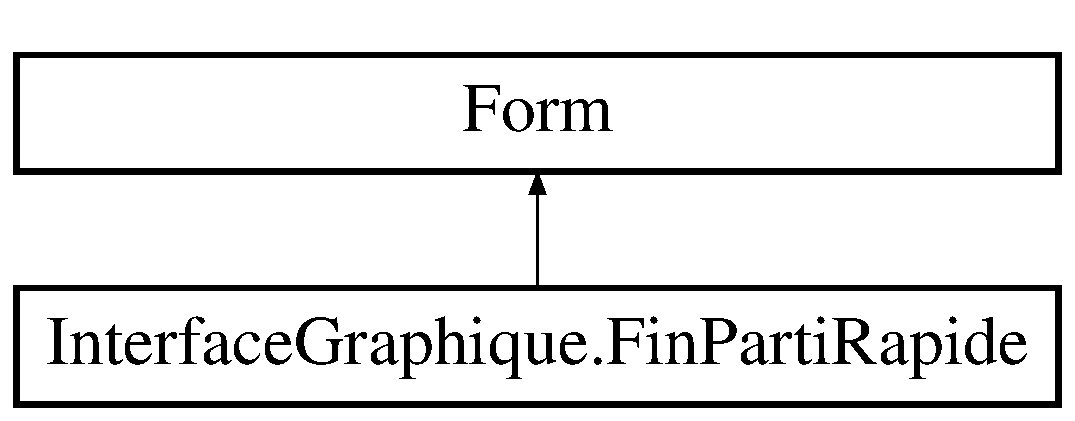
\includegraphics[height=2.000000cm]{class_interface_graphique_1_1_fin_parti_rapide}
\end{center}
\end{figure}
\subsection*{Public Member Functions}
\begin{DoxyCompactItemize}
\item 
void {\bfseries nom\+Vainqueur} (bool vainqueur)
\item 
void {\bfseries score\+Final} (int perdant)
\end{DoxyCompactItemize}
\subsection*{Protected Member Functions}
\begin{DoxyCompactItemize}
\item 
override void \hyperlink{class_interface_graphique_1_1_fin_parti_rapide_a8134ad235e3ceac7c4f6bb06ae168972}{Dispose} (bool disposing)
\begin{DoxyCompactList}\small\item\em Clean up any resources being used. \end{DoxyCompactList}\end{DoxyCompactItemize}


\subsection{Member Function Documentation}
\hypertarget{class_interface_graphique_1_1_fin_parti_rapide_a8134ad235e3ceac7c4f6bb06ae168972}{}\label{class_interface_graphique_1_1_fin_parti_rapide_a8134ad235e3ceac7c4f6bb06ae168972} 
\index{Interface\+Graphique\+::\+Fin\+Parti\+Rapide@{Interface\+Graphique\+::\+Fin\+Parti\+Rapide}!Dispose@{Dispose}}
\index{Dispose@{Dispose}!Interface\+Graphique\+::\+Fin\+Parti\+Rapide@{Interface\+Graphique\+::\+Fin\+Parti\+Rapide}}
\subsubsection{\texorpdfstring{Dispose()}{Dispose()}}
{\footnotesize\ttfamily override void Interface\+Graphique.\+Fin\+Parti\+Rapide.\+Dispose (\begin{DoxyParamCaption}\item[{bool}]{disposing }\end{DoxyParamCaption})\hspace{0.3cm}{\ttfamily [inline]}, {\ttfamily [protected]}}



Clean up any resources being used. 


\begin{DoxyParams}{Parameters}
{\em disposing} & true if managed resources should be disposed; otherwise, false.\\
\hline
\end{DoxyParams}


The documentation for this class was generated from the following files\+:\begin{DoxyCompactItemize}
\item 
Sources/\+Interface\+Graphique/\hyperlink{_fin_parti_rapide_8cs}{Fin\+Parti\+Rapide.\+cs}\item 
Sources/\+Interface\+Graphique/Fin\+Parti\+Rapide.\+Designer.\+cs\end{DoxyCompactItemize}

\hypertarget{class_interface_graphique_1_1_fonctions_natives}{}\section{Interface\+Graphique.\+Fonctions\+Natives Class Reference}
\label{class_interface_graphique_1_1_fonctions_natives}\index{Interface\+Graphique.\+Fonctions\+Natives@{Interface\+Graphique.\+Fonctions\+Natives}}
\subsection*{Classes}
\begin{DoxyCompactItemize}
\item 
struct \hyperlink{struct_interface_graphique_1_1_fonctions_natives_1_1_message}{Message}
\end{DoxyCompactItemize}
\subsection*{Public Member Functions}
\begin{DoxyCompactItemize}
\item 
static bool {\bfseries Peek\+Message} (out \hyperlink{struct_interface_graphique_1_1_fonctions_natives_1_1_message}{Message} message, Int\+Ptr h\+Wnd, uint filter\+Min, uint filter\+Max, uint flags)
\item 
static bool {\bfseries executer\+Tests} ()
\item 
static void {\bfseries initialiser\+Open\+GL} (Int\+Ptr handle)
\item 
static void {\bfseries liberer\+Open\+GL} ()
\item 
static void {\bfseries dessiner\+Open\+GL} ()
\item 
static void {\bfseries animer} (double temps)
\item 
static void {\bfseries redessiner} ()
\item 
static bool {\bfseries ajouter\+Nouveau\+Element} (string nom, int x, int y)
\item 
static bool {\bfseries ajouter\+Nouveau\+Portail} (string nom, int x, int y)
\item 
static bool {\bfseries zoom\+In} ()
\item 
static bool {\bfseries zoom\+Out} ()
\item 
static void {\bfseries redimensionner\+Fenetre} (int x, int y)
\item 
static bool {\bfseries ajouter\+Noeud} (string nom, int x, int y)
\item 
static void {\bfseries initialiser\+Rectangle\+Elas} (int x, int y)
\item 
static void {\bfseries mettre\+A\+Jour\+Rectangle\+Elas} (int x1, int y1)
\item 
static void {\bfseries terminer\+Rectangle\+Elas} ()
\item 
static void {\bfseries dupliquer\+Selection} (int x, int y)
\item 
static void {\bfseries supprimer\+Selection} ()
\item 
static void {\bfseries deplacer\+Selection} (int x, int y)
\item 
static void {\bfseries deselectionner\+Tout} ()
\item 
static void {\bfseries selectionner\+Tout} ()
\item 
static void {\bfseries effacer\+Selection} ()
\item 
static void {\bfseries modifier\+Etat\+C\+T\+RL} (bool etat\+C\+T\+RL)
\item 
static int {\bfseries selectionner\+Objet} (int id, int posX, int posY)
\item 
static void {\bfseries marquer\+Selection} (int id, bool en\+Inverse)
\item 
static void {\bfseries mise\+A\+Echelle} (int x, int y)
\item 
static void {\bfseries initialiser\+Rotation} (int pointY)
\item 
static void {\bfseries initialiser\+Deplacement} (int pointX, int pointY)
\item 
static void {\bfseries effectuer\+Rotation} (int pointY)
\item 
static void {\bfseries effectuer\+Deplacement} (float pointX, float pointY)
\item 
static void {\bfseries selection\+Objet} (int posX, int posY, bool selection\+Unique)
\item 
static double {\bfseries obtenir\+Friction\+Table} ()
\item 
static double {\bfseries obtenir\+Acceleration\+Bonus} ()
\item 
static double {\bfseries obtenir\+Coef\+Rebondissement} ()
\item 
static void {\bfseries friction\+Table\+Bouton} (double friction\+Table)
\item 
static void {\bfseries acceleration\+Bonus\+Bouton} (double acceleration\+Bonus)
\item 
static void {\bfseries coef\+Rebondissement\+Bouton} (double coef\+Rebondissement)
\item 
static int {\bfseries obtenir\+Position\+ObjetX} ()
\item 
static int {\bfseries obtenir\+Position\+ObjetY} ()
\item 
static int {\bfseries obtenir\+Position\+ObjetZ} ()
\item 
static int {\bfseries obtenir\+Angle\+Rotation\+Objet} ()
\item 
static double {\bfseries obtenir\+Facteur\+Echelle\+Objet} ()
\item 
static void {\bfseries mettre\+Echelle\+Objet\+Bouton} (double facteur)
\item 
static void {\bfseries rotation\+Objet\+Bouton} (int angle)
\item 
static void {\bfseries deplacement\+Objet\+Bouton} (float pointX, float pointY)
\item 
static void {\bfseries sauvegarde\+Par\+Defaut} ()
\item 
static void {\bfseries initialisation\+Par\+Defaut} ()
\item 
static void {\bfseries sauvegarder\+Arbre} (string nom\+Fichier)
\item 
static void {\bfseries initialiser\+Chargement} (string nom\+Fichier)
\item 
static void {\bfseries deplacer\+XY} (double deplacementX, double deplacementY)
\item 
static void {\bfseries zoom\+In\+Elas} ()
\item 
static void {\bfseries zoom\+Out\+Elas} ()
\item 
static void {\bfseries selection\+Elastique} ()
\item 
static void {\bfseries charger\+Configuration\+Options} ()
\item 
static void {\bfseries mise\+A\+Jour\+Sauvegarde\+Configuration} (bool peut\+Afficher\+Debogage, bool peut\+Afficher\+Collision, bool peut\+Afficher\+Vitesse\+Rondelle, bool peut\+Afficher\+Eclairage, bool peut\+Afficher\+Attraction\+Portail, int nb\+Buts, string haut, string bas, string gauche, string droite, bool est\+Virtuel)
\item 
static void {\bfseries mise\+A\+Jour\+Chargement\+Configuration} (bool peut\+Afficher\+Debogage, bool peut\+Afficher\+Collision, bool peut\+Afficher\+Vitesse\+Rondelle, bool peut\+Afficher\+Eclairage, bool peut\+Afficher\+Attraction\+Portail, int nb\+Buts, string haut, string bas, string gauche, string droite, bool est\+Virtuel)
\item 
static void {\bfseries sauvegarder\+Configuration\+Options} (string haut, string bas, string gauche, string droite)
\item 
static bool {\bfseries obtenir\+Peut\+Afficher\+Debogage} ()
\item 
static bool {\bfseries obtenir\+Peut\+Afficher\+Collision} ()
\item 
static bool {\bfseries obtenir\+Peut\+Afficher\+Vitesse} ()
\item 
static bool {\bfseries obtenir\+Peut\+Afficher\+Eclairage} ()
\item 
static bool {\bfseries obtenir\+Peut\+Afficher\+Attraction\+Portail} ()
\item 
static int {\bfseries obtenir\+Nb\+Buts} ()
\item 
static Int\+Ptr {\bfseries obtenir\+Haut} ()
\item 
static Int\+Ptr {\bfseries obtenir\+Bas} ()
\item 
static Int\+Ptr {\bfseries obtenir\+Gauche} ()
\item 
static Int\+Ptr {\bfseries obtenir\+Droite} ()
\item 
static bool {\bfseries obtenir\+Est\+Virtuel} ()
\item 
static void {\bfseries creer\+Profil} (string nom, int vitesse, int passivite)
\item 
static void {\bfseries ajouter\+Nouveau\+Profil} (string nom, int vitesse, int passivite)
\item 
static void {\bfseries sauvegarde\+Profils} ()
\item 
static void {\bfseries chargement\+Profils} ()
\item 
static void {\bfseries supprimer\+Profil} (string nom)
\item 
static int {\bfseries nombre\+Profils} ()
\item 
static Int\+Ptr {\bfseries nom\+Du\+Profil} (int profil\+Choisi)
\item 
static int {\bfseries vitesse\+Du\+Profil} (int profil\+Choisi)
\item 
static int {\bfseries passivite\+Du\+Profil} (int profil\+Choisi)
\item 
static void {\bfseries reinitialiser\+Profils} ()
\item 
static void {\bfseries ajouter\+Nom\+Profil} (string nom)
\item 
static void {\bfseries initialiser\+Partie} (int nb\+Buts, bool joueur\+Virtuel)
\item 
static void {\bfseries lancer\+Partie\+Rapide} ()
\item 
static void {\bfseries lancer\+Partie\+Tournoi} (string nom1, string nom2)
\item 
static void {\bfseries assigner\+But} (bool joueur1)
\item 
static void {\bfseries initialiser\+Partie\+Tournoi} ()
\item 
static void {\bfseries arreter\+Partie} ()
\item 
static void {\bfseries arreter\+Tournoi} ()
\item 
static void {\bfseries initialiser\+Tournoi} (int but, bool j1, string nom1, bool j2, string nom2, bool j3, string nom3, bool j4, string nom4)
\item 
static void {\bfseries joueur\+Maillet1} (int x, int y)
\item 
static void {\bfseries joueur\+Maillet2} (double x, double y)
\item 
static void {\bfseries next\+Partie} ()
\item 
static void {\bfseries reinitialiser\+Test} ()
\item 
static bool {\bfseries afficher\+Panel\+Rapide} ()
\item 
static bool {\bfseries nom\+Vainqueur\+Partie\+Rapide} ()
\item 
static int {\bfseries score\+Final\+Perdant} ()
\item 
static bool {\bfseries get\+Joueur1\+Passe} ()
\item 
static bool {\bfseries get\+Joueur3\+Passe} ()
\item 
static bool {\bfseries get\+Vainqueur1\+Passe} ()
\item 
static bool {\bfseries get\+Actualiser1} ()
\item 
static bool {\bfseries get\+Actualiser2} ()
\item 
static bool {\bfseries get\+Actualiser3} ()
\item 
static void {\bfseries en\+Mode\+Edition} (bool mode\+Edition)
\item 
static void {\bfseries reinitialiser\+Partie} ()
\item 
static void {\bfseries adversaire\+Virtuel} (bool virtuel)
\item 
static bool {\bfseries joueur\+Virtuel\+Dans\+Partie\+Courante} ()
\item 
static void {\bfseries sauvegarder\+Tournoi} ()
\item 
static void {\bfseries chargement\+Tournoi} ()
\item 
static void {\bfseries assigner\+Joueur1\+Tournoi} (string nom, bool est\+Virtuel, int index)
\item 
static void {\bfseries assigner\+Joueur2\+Tournoi} (string nom, bool est\+Virtuel, int index)
\item 
static void {\bfseries assigner\+Joueur3\+Tournoi} (string nom, bool est\+Virtuel, int index)
\item 
static void {\bfseries assigner\+Joueur4\+Tournoi} (string nom, bool est\+Virtuel, int index)
\item 
static Int\+Ptr {\bfseries obtenir\+Nom\+Joueur1\+Tournoi} ()
\item 
static Int\+Ptr {\bfseries obtenir\+Nom\+Joueur2\+Tournoi} ()
\item 
static Int\+Ptr {\bfseries obtenir\+Nom\+Joueur3\+Tournoi} ()
\item 
static Int\+Ptr {\bfseries obtenir\+Nom\+Joueur4\+Tournoi} ()
\item 
static bool {\bfseries obtenir\+Type\+Joueur1\+Tournoi} ()
\item 
static bool {\bfseries obtenir\+Type\+Joueur2\+Tournoi} ()
\item 
static bool {\bfseries obtenir\+Type\+Joueur3\+Tournoi} ()
\item 
static bool {\bfseries obtenir\+Type\+Joueur4\+Tournoi} ()
\item 
static int {\bfseries obtenir\+Profil\+Joueur1\+Tournoi} ()
\item 
static int {\bfseries obtenir\+Profil\+Joueur2\+Tournoi} ()
\item 
static int {\bfseries obtenir\+Profil\+Joueur3\+Tournoi} ()
\item 
static int {\bfseries obtenir\+Profil\+Joueur4\+Tournoi} ()
\item 
static void {\bfseries initaliser\+Sono} ()
\item 
static void {\bfseries mettre\+En\+Pause} ()
\item 
static void {\bfseries relacher\+Musique} ()
\item 
static void {\bfseries jouer\+Son\+De\+Fond} ()
\item 
static void {\bfseries en\+Mode\+Test} (bool mode\+Edition)
\item 
static void {\bfseries size\+Fenetre} (int x, int y)
\item 
static void {\bfseries temps\+Jouer} (string temps\+Jouer)
\end{DoxyCompactItemize}


The documentation for this class was generated from the following file\+:\begin{DoxyCompactItemize}
\item 
C\+:/\+Users/\+Steven/\+Documents/\+Poly/\+I\+N\+F2990/inf2990-\/06/\+Cadriciel\+\_\+2016-\/3\+\_\+\+Etudiants/\+Cadriciel/\+Sources/\+Interface\+Graphique/\hyperlink{_fonctions_natives_8cs}{Fonctions\+Natives.\+cs}\end{DoxyCompactItemize}

\hypertarget{class_interface_configuration}{}\section{Interface\+Configuration Class Reference}
\label{class_interface_configuration}\index{Interface\+Configuration@{Interface\+Configuration}}
\subsection*{Public Member Functions}
\begin{DoxyCompactItemize}
\item 
\hyperlink{group__inf2990_ga0f610f6a1fb2877f56c88bfdb32b7232}{Interface\+Configuration} ()
\begin{DoxyCompactList}\small\item\em Constructeur par defaut. \end{DoxyCompactList}\item 
bool \hyperlink{group__inf2990_gad2f726db7e0b3a79737abf30f19cfd71}{obtenir\+Peut\+Afficher\+Debogage} ()
\begin{DoxyCompactList}\small\item\em Retourne s\textquotesingle{}il est possible d\textquotesingle{}afficher a la console. \end{DoxyCompactList}\item 
bool \hyperlink{group__inf2990_ga64d970ca095f3721a1a47e2da00fa3f8}{obtenir\+Peut\+Afficher\+Collision} ()
\begin{DoxyCompactList}\small\item\em Retourne s\textquotesingle{}il est possible d\textquotesingle{}afficher le type d\textquotesingle{}objet entre en collision avec la rondelle. \end{DoxyCompactList}\item 
bool \hyperlink{group__inf2990_ga8dc2c7833c29e8b3162bfdef96a6437d}{obtenir\+Peut\+Afficher\+Vitesse\+Rondelle} ()
\begin{DoxyCompactList}\small\item\em Retourne s\textquotesingle{}il est possible d\textquotesingle{}afficher la vitesse d\textquotesingle{}une rondelle apres collision. \end{DoxyCompactList}\item 
bool \hyperlink{group__inf2990_ga64fc6c1c5b78045184a79888a0eea801}{obtenir\+Peut\+Afficher\+Eclairage} ()
\begin{DoxyCompactList}\small\item\em Retourne si l\textquotesingle{}etat de l\textquotesingle{}eclairage est afficher. \end{DoxyCompactList}\item 
bool \hyperlink{group__inf2990_ga4282f01c1d291050c15ab7402dea129a}{obtenir\+Peut\+Afficher\+Attraction\+Portail} ()
\begin{DoxyCompactList}\small\item\em Retourne si la delimitation de l\textquotesingle{}attraction du portail est affichee. \end{DoxyCompactList}\item 
int \hyperlink{group__inf2990_ga8d60ea6dee12a1b82d36274ad9e6362c}{obtenir\+Nb\+Buts} ()
\begin{DoxyCompactList}\small\item\em Retourne le nombre de buts necessaire pour gagner. \end{DoxyCompactList}\item 
bool \hyperlink{group__inf2990_gac7e5058bb5a2b80a640f102458af9537}{obtenir\+Est\+Virtuel} ()
\begin{DoxyCompactList}\small\item\em Retourne si le deuxieme joueur est virtuel ou non. \end{DoxyCompactList}\item 
void \hyperlink{group__inf2990_ga509d6c5ea4660a58257e56f720ac763b}{modifier\+Peut\+Afficher\+Debogage} (bool peut\+Afficher\+Debogage)
\begin{DoxyCompactList}\small\item\em Modifie l\textquotesingle{}etat de l\textquotesingle{}affichage a la console. \end{DoxyCompactList}\item 
void \hyperlink{group__inf2990_gad1c7d8114fb35937d2490fc517f97838}{modifier\+Peut\+Afficher\+Collision} (bool peut\+Afficher\+Collision)
\begin{DoxyCompactList}\small\item\em Modifie l\textquotesingle{}affichage des collisions. \end{DoxyCompactList}\item 
void \hyperlink{group__inf2990_ga57d4438f62d1c44409b00b3ae8fcc813}{modifier\+Peut\+Afficher\+Vitesse\+Rondelle} (bool peut\+Afficher\+Vitesse)
\begin{DoxyCompactList}\small\item\em Modifie l\textquotesingle{}affichage de la vitesse de la rondelle. \end{DoxyCompactList}\item 
void \hyperlink{group__inf2990_ga5ccb734c81a1dbb22f6043417daffc67}{modifier\+Peut\+Afficher\+Eclairage} (bool peut\+Afficher\+Eclairage)
\begin{DoxyCompactList}\small\item\em Modifie l\textquotesingle{}affichage de l\textquotesingle{}eclairage. \end{DoxyCompactList}\item 
void \hyperlink{group__inf2990_ga5ed1955471ea5a179b61d7f921603d26}{modifier\+Peut\+Afficher\+Attraction\+Portail} (bool peut\+Afficher\+Attraction\+Portail)
\begin{DoxyCompactList}\small\item\em Modifie l\textquotesingle{}affichage de l\textquotesingle{}attraction des portails. \end{DoxyCompactList}\item 
void \hyperlink{group__inf2990_ga570191806ecab091e74861a8a01f1ff9}{modifier\+Nb\+Buts} (int nb\+Buts)
\begin{DoxyCompactList}\small\item\em Modifie le nombre de buts necessaires pour gagner. \end{DoxyCompactList}\item 
void \hyperlink{group__inf2990_ga80f804298396f27f820928b7fb72ebfd}{modifier\+Est\+Virtuel} (bool est\+Virtuel)
\begin{DoxyCompactList}\small\item\em Modifie le type de joueur (virtuel ou non) \end{DoxyCompactList}\end{DoxyCompactItemize}


The documentation for this class was generated from the following files\+:\begin{DoxyCompactItemize}
\item 
Sources/\+D\+L\+L/\hyperlink{_interface_configuration_8h}{Interface\+Configuration.\+h}\item 
Sources/\+D\+L\+L/Interface\+Configuration.\+cpp\end{DoxyCompactItemize}

\hypertarget{struct_interface_graphique_1_1_program_1_1_joueur}{}\section{Interface\+Graphique.\+Program.\+Joueur Struct Reference}
\label{struct_interface_graphique_1_1_program_1_1_joueur}\index{Interface\+Graphique.\+Program.\+Joueur@{Interface\+Graphique.\+Program.\+Joueur}}
\subsection*{Public Member Functions}
\begin{DoxyCompactItemize}
\item 
\hypertarget{struct_interface_graphique_1_1_program_1_1_joueur_aaf155cedd23600e18f16c434489eb534}{}\label{struct_interface_graphique_1_1_program_1_1_joueur_aaf155cedd23600e18f16c434489eb534} 
{\bfseries Joueur} (string c\+Nom, bool c\+Est\+Virtuel, \hyperlink{struct_interface_graphique_1_1_profil}{Profil} c\+Profil)
\end{DoxyCompactItemize}
\subsection*{Public Attributes}
\begin{DoxyCompactItemize}
\item 
\hypertarget{struct_interface_graphique_1_1_program_1_1_joueur_ad063811f744eed615e20751876026835}{}\label{struct_interface_graphique_1_1_program_1_1_joueur_ad063811f744eed615e20751876026835} 
string {\bfseries nom}
\item 
\hypertarget{struct_interface_graphique_1_1_program_1_1_joueur_ad6f62d644a74c223dd80d1da000166d5}{}\label{struct_interface_graphique_1_1_program_1_1_joueur_ad6f62d644a74c223dd80d1da000166d5} 
bool {\bfseries est\+Virtuel}
\item 
\hypertarget{struct_interface_graphique_1_1_program_1_1_joueur_a70160134dded79a4a0fe5ef577ed4875}{}\label{struct_interface_graphique_1_1_program_1_1_joueur_a70160134dded79a4a0fe5ef577ed4875} 
\hyperlink{struct_interface_graphique_1_1_profil}{Profil} {\bfseries profil}
\end{DoxyCompactItemize}


The documentation for this struct was generated from the following file\+:\begin{DoxyCompactItemize}
\item 
C\+:/\+Users/\+Steven/\+Documents/\+Poly/\+I\+N\+F2990/inf2990-\/06/\+Cadriciel\+\_\+2016-\/3\+\_\+\+Etudiants/\+Cadriciel/\+Sources/\+Interface\+Graphique/Program.\+cs\end{DoxyCompactItemize}

\hypertarget{class_interface_graphique_1_1_menu_principal}{}\section{Interface\+Graphique.\+Menu\+Principal Class Reference}
\label{class_interface_graphique_1_1_menu_principal}\index{Interface\+Graphique.\+Menu\+Principal@{Interface\+Graphique.\+Menu\+Principal}}
Inheritance diagram for Interface\+Graphique.\+Menu\+Principal\+:\begin{figure}[H]
\begin{center}
\leavevmode
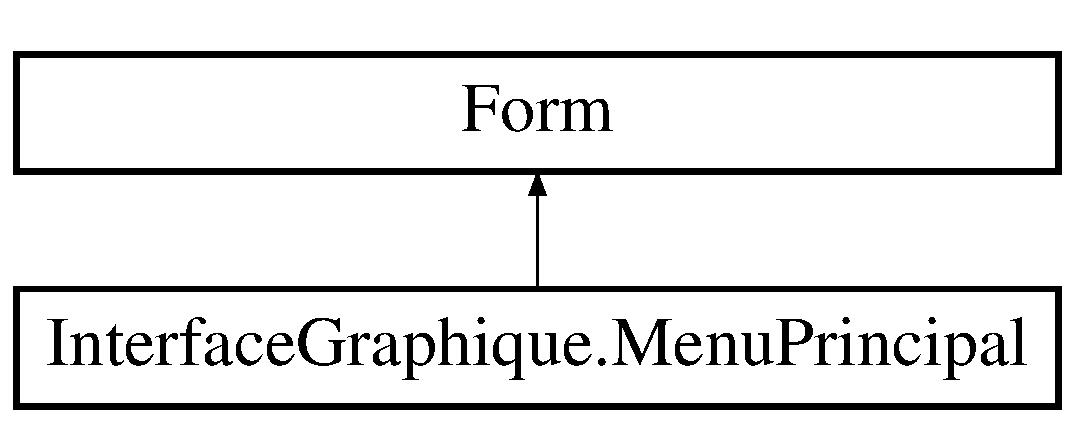
\includegraphics[height=2.000000cm]{class_interface_graphique_1_1_menu_principal}
\end{center}
\end{figure}
\subsection*{Protected Member Functions}
\begin{DoxyCompactItemize}
\item 
override void \hyperlink{class_interface_graphique_1_1_menu_principal_a5a9389c7864e1b29b7520f77606d357d}{Dispose} (bool disposing)
\begin{DoxyCompactList}\small\item\em Clean up any resources being used. \end{DoxyCompactList}\end{DoxyCompactItemize}


\subsection{Member Function Documentation}
\hypertarget{class_interface_graphique_1_1_menu_principal_a5a9389c7864e1b29b7520f77606d357d}{}\label{class_interface_graphique_1_1_menu_principal_a5a9389c7864e1b29b7520f77606d357d} 
\index{Interface\+Graphique\+::\+Menu\+Principal@{Interface\+Graphique\+::\+Menu\+Principal}!Dispose@{Dispose}}
\index{Dispose@{Dispose}!Interface\+Graphique\+::\+Menu\+Principal@{Interface\+Graphique\+::\+Menu\+Principal}}
\subsubsection{\texorpdfstring{Dispose()}{Dispose()}}
{\footnotesize\ttfamily override void Interface\+Graphique.\+Menu\+Principal.\+Dispose (\begin{DoxyParamCaption}\item[{bool}]{disposing }\end{DoxyParamCaption})\hspace{0.3cm}{\ttfamily [inline]}, {\ttfamily [protected]}}



Clean up any resources being used. 


\begin{DoxyParams}{Parameters}
{\em disposing} & true if managed resources should be disposed; otherwise, false.\\
\hline
\end{DoxyParams}


The documentation for this class was generated from the following files\+:\begin{DoxyCompactItemize}
\item 
Sources/\+Interface\+Graphique/\hyperlink{_menu_principal_8cs}{Menu\+Principal.\+cs}\item 
Sources/\+Interface\+Graphique/Menu\+Principal.\+Designer.\+cs\end{DoxyCompactItemize}

\hypertarget{struct_interface_graphique_1_1_fonctions_natives_1_1_message}{}\section{Interface\+Graphique.\+Fonctions\+Natives.\+Message Struct Reference}
\label{struct_interface_graphique_1_1_fonctions_natives_1_1_message}\index{Interface\+Graphique.\+Fonctions\+Natives.\+Message@{Interface\+Graphique.\+Fonctions\+Natives.\+Message}}
\subsection*{Public Attributes}
\begin{DoxyCompactItemize}
\item 
Int\+Ptr {\bfseries h\+Wnd}
\item 
uint {\bfseries Msg}
\item 
Int\+Ptr {\bfseries w\+Param}
\item 
Int\+Ptr {\bfseries l\+Param}
\item 
uint {\bfseries Time}
\item 
System.\+Drawing.\+Point {\bfseries Point}
\end{DoxyCompactItemize}


The documentation for this struct was generated from the following file\+:\begin{DoxyCompactItemize}
\item 
Sources/\+Interface\+Graphique/Fonctions\+Natives.\+cs\end{DoxyCompactItemize}

\hypertarget{class_interface_graphique_1_1_mode_edition}{}\section{Interface\+Graphique.\+Mode\+Edition Class Reference}
\label{class_interface_graphique_1_1_mode_edition}\index{Interface\+Graphique.\+Mode\+Edition@{Interface\+Graphique.\+Mode\+Edition}}
Inheritance diagram for Interface\+Graphique.\+Mode\+Edition\+:\begin{figure}[H]
\begin{center}
\leavevmode
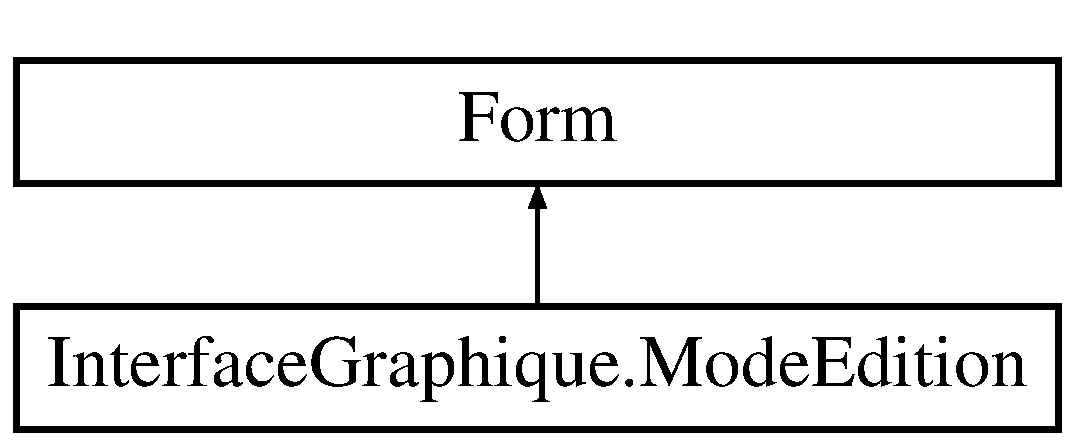
\includegraphics[height=2.000000cm]{class_interface_graphique_1_1_mode_edition}
\end{center}
\end{figure}
\subsection*{Public Member Functions}
\begin{DoxyCompactItemize}
\item 
void {\bfseries Initialiser\+Animation} ()
\item 
void {\bfseries Mettre\+A\+Jour} (double temps\+Inter\+Affichage)
\item 
void {\bfseries lancer\+Mode\+Edition} ()
\end{DoxyCompactItemize}
\subsection*{Static Public Attributes}
\begin{DoxyCompactItemize}
\item 
static bool {\bfseries zoom\+In\+Elas} = false
\item 
static bool {\bfseries zoom\+Out\+Elas} = false
\item 
static bool {\bfseries en\+Echelle} = false
\item 
static bool {\bfseries en\+Rotation} = false
\item 
static bool {\bfseries en\+Deplacement} = false
\item 
static bool {\bfseries en\+Mode\+Test} = false
\end{DoxyCompactItemize}
\subsection*{Protected Member Functions}
\begin{DoxyCompactItemize}
\item 
override bool {\bfseries Process\+Cmd\+Key} (ref Message msg, Keys key\+Data)
\item 
override void \hyperlink{class_interface_graphique_1_1_mode_edition_abcb92e7500b3c90cdc6fcc24ae0c3234}{Dispose} (bool disposing)
\begin{DoxyCompactList}\small\item\em Clean up any resources being used. \end{DoxyCompactList}\end{DoxyCompactItemize}


\subsection{Member Function Documentation}
\hypertarget{class_interface_graphique_1_1_mode_edition_abcb92e7500b3c90cdc6fcc24ae0c3234}{}\label{class_interface_graphique_1_1_mode_edition_abcb92e7500b3c90cdc6fcc24ae0c3234} 
\index{Interface\+Graphique\+::\+Mode\+Edition@{Interface\+Graphique\+::\+Mode\+Edition}!Dispose@{Dispose}}
\index{Dispose@{Dispose}!Interface\+Graphique\+::\+Mode\+Edition@{Interface\+Graphique\+::\+Mode\+Edition}}
\subsubsection{\texorpdfstring{Dispose()}{Dispose()}}
{\footnotesize\ttfamily override void Interface\+Graphique.\+Mode\+Edition.\+Dispose (\begin{DoxyParamCaption}\item[{bool}]{disposing }\end{DoxyParamCaption})\hspace{0.3cm}{\ttfamily [inline]}, {\ttfamily [protected]}}



Clean up any resources being used. 


\begin{DoxyParams}{Parameters}
{\em disposing} & true if managed resources should be disposed; otherwise, false.\\
\hline
\end{DoxyParams}


The documentation for this class was generated from the following files\+:\begin{DoxyCompactItemize}
\item 
Sources/\+Interface\+Graphique/\hyperlink{_mode_edition_8cs}{Mode\+Edition.\+cs}\item 
Sources/\+Interface\+Graphique/Mode\+Edition.\+Designer.\+cs\end{DoxyCompactItemize}

\hypertarget{class_interface_graphique_1_1_mode_test}{}\section{Interface\+Graphique.\+Mode\+Test Class Reference}
\label{class_interface_graphique_1_1_mode_test}\index{Interface\+Graphique.\+Mode\+Test@{Interface\+Graphique.\+Mode\+Test}}
Inheritance diagram for Interface\+Graphique.\+Mode\+Test\+:\begin{figure}[H]
\begin{center}
\leavevmode
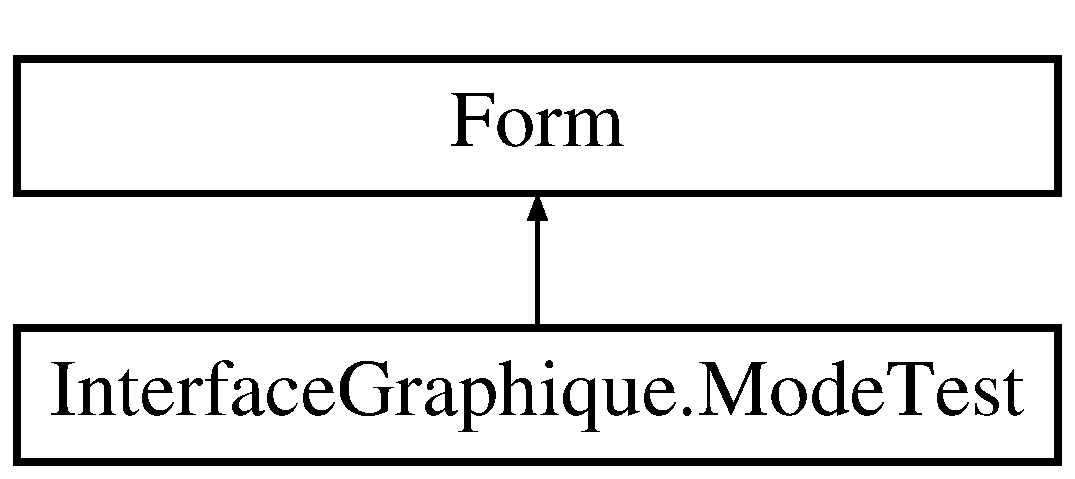
\includegraphics[height=2.000000cm]{class_interface_graphique_1_1_mode_test}
\end{center}
\end{figure}
\subsection*{Public Member Functions}
\begin{DoxyCompactItemize}
\item 
\hypertarget{class_interface_graphique_1_1_mode_test_afb82898571c13159717496bd5ef0f9cd}{}\label{class_interface_graphique_1_1_mode_test_afb82898571c13159717496bd5ef0f9cd} 
void \hyperlink{class_interface_graphique_1_1_mode_test_afb82898571c13159717496bd5ef0f9cd}{Initialiser\+Animation} ()
\begin{DoxyCompactList}\small\item\em Initialiser les animations. \end{DoxyCompactList}\end{DoxyCompactItemize}
\subsection*{Protected Member Functions}
\begin{DoxyCompactItemize}
\item 
\hypertarget{class_interface_graphique_1_1_mode_test_a253fb0ff92405481372471873a088afd}{}\label{class_interface_graphique_1_1_mode_test_a253fb0ff92405481372471873a088afd} 
override bool \hyperlink{class_interface_graphique_1_1_mode_test_a253fb0ff92405481372471873a088afd}{Process\+Cmd\+Key} (ref Message msg, Keys key\+Data)
\begin{DoxyCompactList}\small\item\em Pour afficher la barre de menu avec le bouton E\+SC. \end{DoxyCompactList}\item 
override void \hyperlink{class_interface_graphique_1_1_mode_test_a06f68e45851d96953a8413bd1d85a59c}{Dispose} (bool disposing)
\begin{DoxyCompactList}\small\item\em Clean up any resources being used. \end{DoxyCompactList}\end{DoxyCompactItemize}


\subsection{Member Function Documentation}
\hypertarget{class_interface_graphique_1_1_mode_test_a06f68e45851d96953a8413bd1d85a59c}{}\label{class_interface_graphique_1_1_mode_test_a06f68e45851d96953a8413bd1d85a59c} 
\index{Interface\+Graphique\+::\+Mode\+Test@{Interface\+Graphique\+::\+Mode\+Test}!Dispose@{Dispose}}
\index{Dispose@{Dispose}!Interface\+Graphique\+::\+Mode\+Test@{Interface\+Graphique\+::\+Mode\+Test}}
\subsubsection{\texorpdfstring{Dispose()}{Dispose()}}
{\footnotesize\ttfamily override void Interface\+Graphique.\+Mode\+Test.\+Dispose (\begin{DoxyParamCaption}\item[{bool}]{disposing }\end{DoxyParamCaption})\hspace{0.3cm}{\ttfamily [inline]}, {\ttfamily [protected]}}



Clean up any resources being used. 


\begin{DoxyParams}{Parameters}
{\em disposing} & true if managed resources should be disposed; otherwise, false.\\
\hline
\end{DoxyParams}


The documentation for this class was generated from the following files\+:\begin{DoxyCompactItemize}
\item 
Sources/\+Interface\+Graphique/Mode\+Test.\+cs\item 
Sources/\+Interface\+Graphique/Mode\+Test.\+Designer.\+cs\end{DoxyCompactItemize}

\hypertarget{class_noeud_abstrait}{}\section{Noeud\+Abstrait Class Reference}
\label{class_noeud_abstrait}\index{Noeud\+Abstrait@{Noeud\+Abstrait}}


Classe de base du patron composite utilis�e pour cr�er l\textquotesingle{}arbre de rendu.  




{\ttfamily \#include $<$Noeud\+Abstrait.\+h$>$}

Inheritance diagram for Noeud\+Abstrait\+:\begin{figure}[H]
\begin{center}
\leavevmode
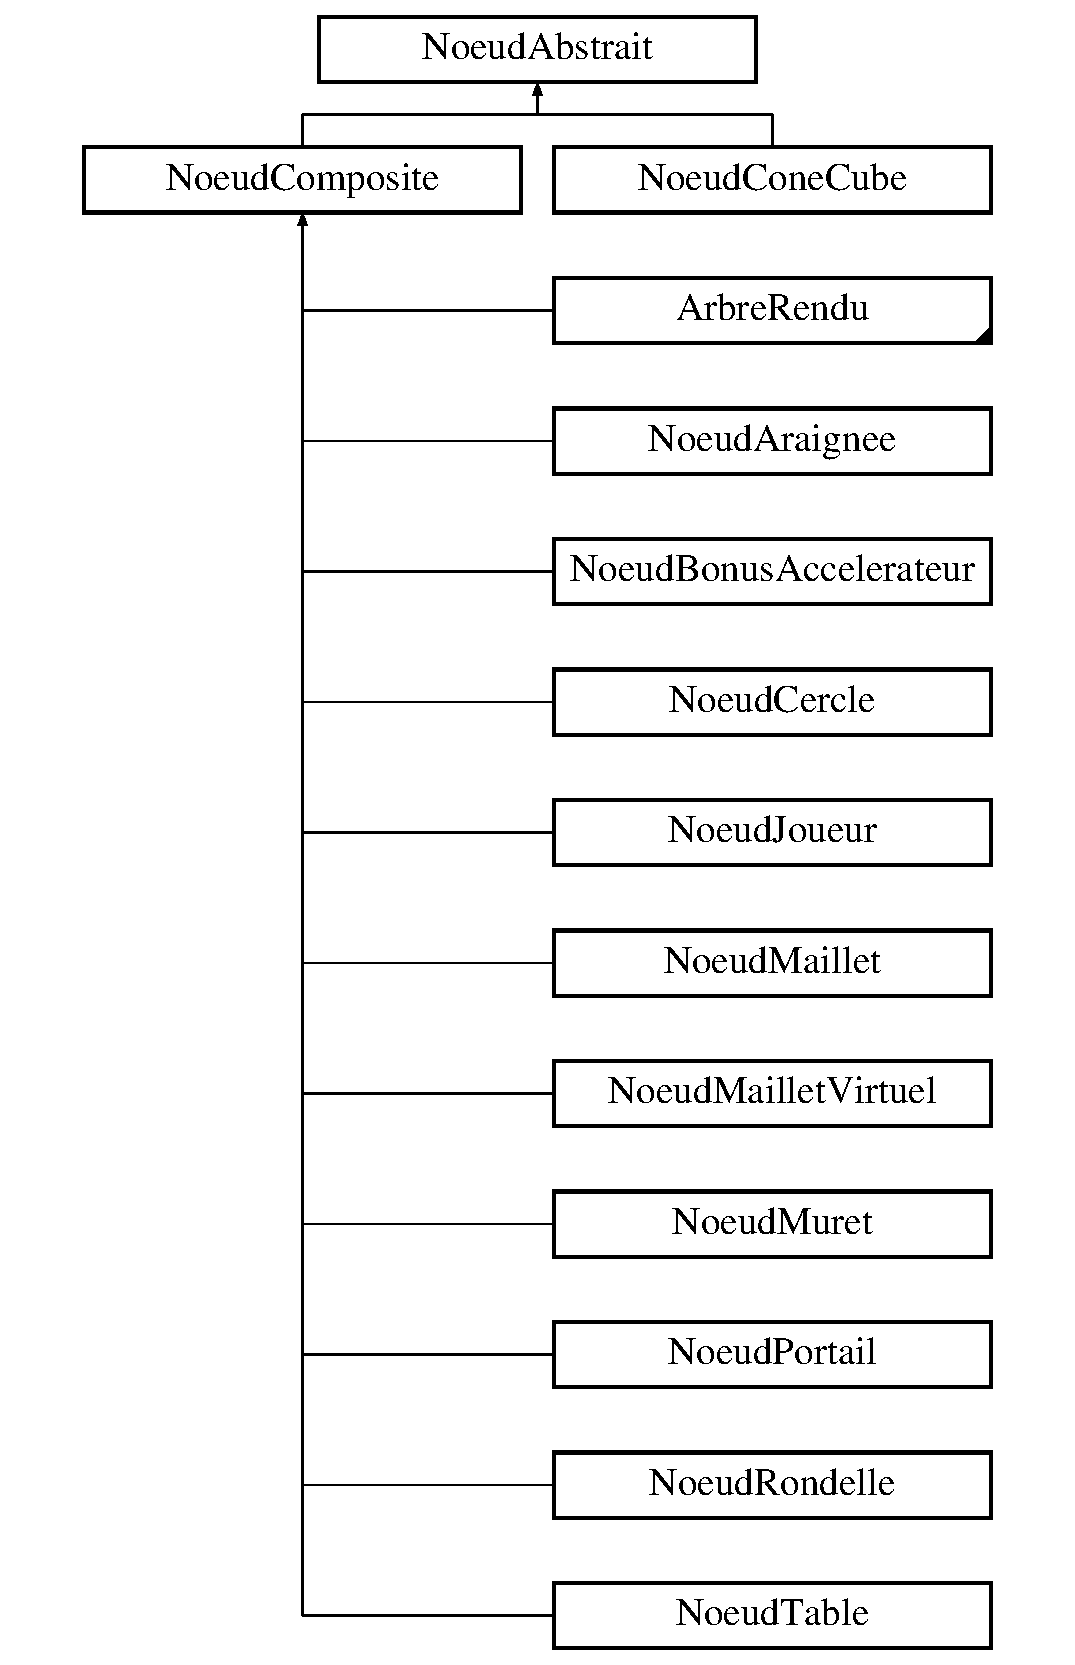
\includegraphics[height=12.000000cm]{class_noeud_abstrait}
\end{center}
\end{figure}
\subsection*{Public Member Functions}
\begin{DoxyCompactItemize}
\item 
\hyperlink{group__inf2990_ga6050aa03c0907f5d227599158ddbd0e7}{Noeud\+Abstrait} (const std\+::string \&type=std\+::string\{ \char`\"{}\char`\"{} \})
\begin{DoxyCompactList}\small\item\em Constructeur. \end{DoxyCompactList}\item 
{\bfseries Noeud\+Abstrait} (const \hyperlink{class_noeud_abstrait}{Noeud\+Abstrait} \&)
\item 
virtual \hyperlink{group__inf2990_ga0ab3f7ab838e8349113da5074abcdc3a}{$\sim$\+Noeud\+Abstrait} ()
\begin{DoxyCompactList}\small\item\em Destructeur. \end{DoxyCompactList}\item 
\hyperlink{class_noeud_abstrait}{Noeud\+Abstrait} $\ast$ \hyperlink{group__inf2990_gaa2ac8c4cd02d88c312b92c65e07ed6d9}{obtenir\+Parent} ()
\begin{DoxyCompactList}\small\item\em Obtient le parent de ce noeud. \end{DoxyCompactList}\item 
const \hyperlink{class_noeud_abstrait}{Noeud\+Abstrait} $\ast$ \hyperlink{group__inf2990_ga46718035b18d5e3c40fe6120114d5160}{obtenir\+Parent} () const
\begin{DoxyCompactList}\small\item\em Obtient le parent de ce noeud (version constante). \end{DoxyCompactList}\item 
void \hyperlink{group__inf2990_ga7787ab59ecc1e6119287459a7154f307}{assigner\+Parent} (\hyperlink{class_noeud_abstrait}{Noeud\+Abstrait} $\ast$parent)
\begin{DoxyCompactList}\small\item\em Assigne le parent de ce noeud. \end{DoxyCompactList}\item 
glm\+::vec3 \hyperlink{group__inf2990_ga4a11b29326d8790c28edd621410f3397}{obtenir\+Position\+Relative} () const
\begin{DoxyCompactList}\small\item\em Obtient la position relative du noeud. \end{DoxyCompactList}\item 
glm\+::vec3 \hyperlink{group__inf2990_gaa57ab777a44551aba400a3cf85c99bf5}{obtenir\+Position\+Initial} () const
\begin{DoxyCompactList}\small\item\em Obtient la position initial du noeud. \end{DoxyCompactList}\item 
void \hyperlink{group__inf2990_ga8386fa98c98908b4d64dd50fb9ba578e}{assigner\+Position\+Relative} (const glm\+::vec3 \&position\+Relative)
\begin{DoxyCompactList}\small\item\em Assigne la position relative du noeud. \end{DoxyCompactList}\item 
void \hyperlink{group__inf2990_ga0a31c874f760457b85b9a195d9486d22}{assigner\+Position\+Initial} (const glm\+::dvec3 \&position\+Initial)
\begin{DoxyCompactList}\small\item\em Assigne la position initial du noeud. \end{DoxyCompactList}\item 
const std\+::string \& \hyperlink{group__inf2990_ga27b387a48de49812a1c3bc5cb35ec8cb}{obtenir\+Type} () const
\begin{DoxyCompactList}\small\item\em Obtient le type du noeud. \end{DoxyCompactList}\item 
void \hyperlink{group__inf2990_gad5205d1e1b63fb66175a8580261d5eea}{assigner\+Affiche} (bool affiche)
\begin{DoxyCompactList}\small\item\em �crit l\textquotesingle{}�tat de l\textquotesingle{}affichage du du noeud. \end{DoxyCompactList}\item 
bool \hyperlink{group__inf2990_ga8e2305abde7e3cf2a99028e0e4982f23}{est\+Affiche} () const
\begin{DoxyCompactList}\small\item\em V�rifie si le noeud se fait afficher. \end{DoxyCompactList}\item 
void \hyperlink{group__inf2990_ga0f39647390d357d8662a870f0c76242c}{assigner\+Selection} (bool selectionne)
\begin{DoxyCompactList}\small\item\em �crit l\textquotesingle{}�tat de la s�lection du noeud. \end{DoxyCompactList}\item 
bool \hyperlink{group__inf2990_ga7e637f6ac30a98c03504385e0f3ef8b8}{est\+Selectionne} () const
\begin{DoxyCompactList}\small\item\em V�rifie si le noeud est s�lectionn�. \end{DoxyCompactList}\item 
void \hyperlink{group__inf2990_ga397add0bac7ec3b842598a2085990b7d}{assigner\+Est\+Selectionnable} (bool selectionnable)
\begin{DoxyCompactList}\small\item\em �crit si le noeud peut �tre s�lectionn� ou non. \end{DoxyCompactList}\item 
bool \hyperlink{group__inf2990_gafe6d0f5f21e222d5cb1dce947c0350cd}{est\+Selectionnable} () const
\begin{DoxyCompactList}\small\item\em V�rifie si le noeud est s�lectionnable. \end{DoxyCompactList}\item 
void \hyperlink{group__inf2990_gabb7f3756a4094dc588690126ec0703d3}{assigner\+Est\+Enregistrable} (bool enregistrable)
\begin{DoxyCompactList}\small\item\em �crit si le noeud peut �tre enregistr� ou non. \end{DoxyCompactList}\item 
bool \hyperlink{group__inf2990_gad5406d04d35203139885f087a657c693}{est\+Enregistrable} () const
\begin{DoxyCompactList}\small\item\em V�rifie si le noeud est enregistrable. \end{DoxyCompactList}\item 
virtual void \hyperlink{group__inf2990_ga1f533acce98fbad7fa82758ccaea55ff}{assigner\+Objet\+Rendu} (modele\+::\+Modele3D const $\ast$modele, opengl\+::\+V\+BO const $\ast$liste)
\begin{DoxyCompactList}\small\item\em Assigne le mod�le3D et la liste d\textquotesingle{}affichage du noeud courant. \end{DoxyCompactList}\item 
const modele\+::\+Modele3D $\ast$ {\bfseries obtenir\+Modele} () const
\item 
modele\+::\+Modele3D $\ast$ {\bfseries obtenir\+Modele} ()
\item 
virtual unsigned int \hyperlink{group__inf2990_ga3224960a3448b73578c6da95dc2dfc13}{calculer\+Profondeur} () const
\begin{DoxyCompactList}\small\item\em Calcule la profondeur de l\textquotesingle{}arbre sous le noeud courant. \end{DoxyCompactList}\item 
virtual void \hyperlink{group__inf2990_ga55435ee83860c6a2101334ba67bbd9b6}{vider} ()
\begin{DoxyCompactList}\small\item\em Vide le noeud de ses enfants. \end{DoxyCompactList}\item 
virtual void \hyperlink{group__inf2990_ga2ab3dc520026d1ad77aa848981688bfd}{effacer} (const \hyperlink{class_noeud_abstrait}{Noeud\+Abstrait} $\ast$noeud)
\begin{DoxyCompactList}\small\item\em Efface le noeud pass� en param�tre. \end{DoxyCompactList}\item 
virtual const \hyperlink{class_noeud_abstrait}{Noeud\+Abstrait} $\ast$ \hyperlink{group__inf2990_ga5ff87ce45a4cb74850e487f6eb4a1b35}{chercher} (const std\+::string \&type\+Noeud) const
\begin{DoxyCompactList}\small\item\em Cherche un noeud par le type (sur un noeud constant). \end{DoxyCompactList}\item 
virtual \hyperlink{class_noeud_abstrait}{Noeud\+Abstrait} $\ast$ \hyperlink{group__inf2990_ga0868ae108165b071f6c8a68a7265c770}{chercher} (const std\+::string \&type\+Noeud)
\begin{DoxyCompactList}\small\item\em Cherche un noeud par le type. \end{DoxyCompactList}\item 
virtual const \hyperlink{class_noeud_abstrait}{Noeud\+Abstrait} $\ast$ \hyperlink{group__inf2990_gadd3954d0d5f9d18d3a94bfe9a522d7d9}{chercher} (unsigned int indice) const
\begin{DoxyCompactList}\small\item\em Cherche un noeud enfant selon l\textquotesingle{}indice (sur un noeud constant). \end{DoxyCompactList}\item 
virtual \hyperlink{class_noeud_abstrait}{Noeud\+Abstrait} $\ast$ \hyperlink{group__inf2990_ga13f7e9a637f7439b1a0cec0c49f6fa88}{chercher} (unsigned int indice)
\begin{DoxyCompactList}\small\item\em Cherche un noeud enfant selon l\textquotesingle{}indice. \end{DoxyCompactList}\item 
virtual bool \hyperlink{group__inf2990_ga31dd45110fcb977a956a32b918f71819}{ajouter} (\hyperlink{class_noeud_abstrait}{Noeud\+Abstrait} $\ast$enfant)
\begin{DoxyCompactList}\small\item\em Ajoute un noeud enfant. \end{DoxyCompactList}\item 
virtual unsigned int \hyperlink{group__inf2990_ga4e135461e8c6a5eaef05c5cbcc3e2679}{obtenir\+Nombre\+Enfants} () const
\begin{DoxyCompactList}\small\item\em Obtient le nombre d\textquotesingle{}enfants du noeud. \end{DoxyCompactList}\item 
virtual void \hyperlink{class_noeud_abstrait_a11dd35de4e64d006e0a869ae618b5f8d}{accepter\+Visiteur} (\hyperlink{class_visiteur_abstrait}{Visiteur\+Abstrait} $\ast$visiteur)
\item 
virtual void {\bfseries attribuer\+Couleur\+Selection} ()
\item 
\hypertarget{class_noeud_abstrait_a57db1361272b748ef3ff35af91bc34cc}{}\label{class_noeud_abstrait_a57db1361272b748ef3ff35af91bc34cc} 
virtual bool {\bfseries verifier\+Selection} (G\+Lubyte couleur\+Back\mbox{[}$\,$\mbox{]})
\item 
virtual void \hyperlink{group__inf2990_ga2516eef94f98d4951baff6fd45020725}{inverser\+Selection} ()
\begin{DoxyCompactList}\small\item\em Changer la s�lection du noeud. \end{DoxyCompactList}\item 
virtual void \hyperlink{group__inf2990_gaf6440c1b4ab6861f0ace6ba410c1fc84}{effacer\+Selection} ()
\begin{DoxyCompactList}\small\item\em Efface les enfants s�lectionn�s. \end{DoxyCompactList}\item 
virtual void \hyperlink{group__inf2990_gaa9b1fa06dad2695ea6870411c62652b3}{selectionner\+Tout} ()
\begin{DoxyCompactList}\small\item\em S�lectionne tous les enfants de m�me que le noeud. \end{DoxyCompactList}\item 
virtual void \hyperlink{group__inf2990_ga4f942bd122fc3402537ecac737c5248a}{deselectionner\+Tout} ()
\begin{DoxyCompactList}\small\item\em D�s�lectionne tous les enfants de m�me que le noeud. \end{DoxyCompactList}\item 
virtual bool \hyperlink{group__inf2990_gabc5c24b3f93c8f1a80b3d632e5848506}{selection\+Existe} () const
\begin{DoxyCompactList}\small\item\em V�rifier si le noeud ou un de ses enfants est s�lectionn�. \end{DoxyCompactList}\item 
virtual void \hyperlink{group__inf2990_ga13a97383c2081b405fc2e0d97cff80df}{changer\+Mode\+Polygones} (bool est\+Force)
\begin{DoxyCompactList}\small\item\em Change le mode d\textquotesingle{}affichage des polygones. \end{DoxyCompactList}\item 
virtual void \hyperlink{group__inf2990_ga726d9d0a524939f405aeeac3fbd06666}{assigner\+Mode\+Polygones} (G\+Lenum mode\+Polygones)
\begin{DoxyCompactList}\small\item\em Assigne le mode d\textquotesingle{}affichage des polygones. \end{DoxyCompactList}\item 
virtual void \hyperlink{group__inf2990_ga7b61f3fcf39176bc4683e15a773c4900}{afficher} (const glm\+::mat4 \&vue\+Projection, const bool \&attribuer\+Couleur) const
\begin{DoxyCompactList}\small\item\em Affiche le noeud. \end{DoxyCompactList}\item 
virtual void \hyperlink{group__inf2990_gaa2ce9ca90a527d7070fddae27a201228}{afficher\+Concret} (const glm\+::mat4 \&vue\+Projection, const bool \&attribuer\+Couleur) const
\begin{DoxyCompactList}\small\item\em Affiche le noeud de mani�re concr�te. \end{DoxyCompactList}\item 
virtual void \hyperlink{group__inf2990_gadc6ebe69894dbb682fdd0ecb1b6c11e9}{animer} (float dt)
\begin{DoxyCompactList}\small\item\em Anime le noeud. \end{DoxyCompactList}\item 
virtual void {\bfseries redessiner} ()
\item 
\hypertarget{class_noeud_abstrait_a63fae34d539d97ca227afeeb6eb53fb2}{}\label{class_noeud_abstrait_a63fae34d539d97ca227afeeb6eb53fb2} 
virtual void {\bfseries redefinir\+Sommets} ()
\item 
\hypertarget{class_noeud_abstrait_a44a94915b16d4c3b9292ad3dbbc7c9fd}{}\label{class_noeud_abstrait_a44a94915b16d4c3b9292ad3dbbc7c9fd} 
virtual bool {\bfseries curseur\+Est\+Dans\+Table} (glm\+::dvec3 pos)
\item 
\hypertarget{class_noeud_abstrait_a338b514befd6fcf916462452778e7e33}{}\label{class_noeud_abstrait_a338b514befd6fcf916462452778e7e33} 
virtual bool {\bfseries curseur\+Est\+Dans\+Zone} (glm\+::dvec3 pos)
\item 
\hypertarget{class_noeud_abstrait_ad1fb3d9abd2f132ea03c5bfaad9e9745}{}\label{class_noeud_abstrait_ad1fb3d9abd2f132ea03c5bfaad9e9745} 
virtual bool \hyperlink{class_noeud_abstrait_ad1fb3d9abd2f132ea03c5bfaad9e9745}{est\+Dans\+La\+Table} ()
\begin{DoxyCompactList}\small\item\em permet de verifier si un objet est toujours a l\textquotesingle{}interieur de la table. \end{DoxyCompactList}\item 
\hypertarget{class_noeud_abstrait_a4cb62bc7f8dc507263a46650e4183056}{}\label{class_noeud_abstrait_a4cb62bc7f8dc507263a46650e4183056} 
virtual bool \hyperlink{class_noeud_abstrait_a4cb62bc7f8dc507263a46650e4183056}{dans\+La\+Table\+Si\+Selectionne} ()
\begin{DoxyCompactList}\small\item\em permet de verifier si un objet selectionn� est toujours a l\textquotesingle{}interieur de la table \end{DoxyCompactList}\item 
\hypertarget{class_noeud_abstrait_a982041848e48b69ca596e263d42dd09c}{}\label{class_noeud_abstrait_a982041848e48b69ca596e263d42dd09c} 
virtual void {\bfseries assigner\+Est\+Visite} (const bool \&est\+Visite)
\item 
\hypertarget{class_noeud_abstrait_a4a06bb8a2d7b3b859caf72c69d86c6f7}{}\label{class_noeud_abstrait_a4a06bb8a2d7b3b859caf72c69d86c6f7} 
virtual float {\bfseries obtenir\+Rayon} () const
\item 
\hypertarget{class_noeud_abstrait_a72a751780f8c101639e4295536da1528}{}\label{class_noeud_abstrait_a72a751780f8c101639e4295536da1528} 
virtual void {\bfseries modifier\+Rayon} (float rayon)
\item 
const vector$<$ glm\+::dvec3 $>$ \& {\bfseries obtenir\+Sommets} ()
\item 
void {\bfseries assigner\+Sommets} (vector$<$ glm\+::dvec3 $>$ \&sommets)
\item 
\hypertarget{class_noeud_abstrait_a78cb5837baaf89684a64c8183859b936}{}\label{class_noeud_abstrait_a78cb5837baaf89684a64c8183859b936} 
int {\bfseries obtenir\+Id} ()
\item 
\hypertarget{class_noeud_abstrait_af3eb8620b887cf2494a6265020d96c0c}{}\label{class_noeud_abstrait_af3eb8620b887cf2494a6265020d96c0c} 
void {\bfseries modifier\+Id} (int id)
\item 
\hypertarget{class_noeud_abstrait_a2b5a3171060ab4d7947dad76f607cb94}{}\label{class_noeud_abstrait_a2b5a3171060ab4d7947dad76f607cb94} 
void {\bfseries modifier\+V\+BO} (opengl\+::\+V\+BO const $\ast$vbo\+Selec)
\item 
\hypertarget{class_noeud_abstrait_a2d856543910d3c399095ab62cfa1ffac}{}\label{class_noeud_abstrait_a2d856543910d3c399095ab62cfa1ffac} 
opengl\+::\+V\+BO const  $\ast$ {\bfseries obtenir\+V\+BO} ()
\item 
double \hyperlink{group__inf2990_gadda2f53142bde30df47677acc842259c}{obtenir\+Angle\+Rotation} ()
\item 
void \hyperlink{group__inf2990_ga0a62efedf581f316a0b8cb22dc4ac547}{modifier\+Angle\+Rotation} (double angle\+Rotation)
\item 
double {\bfseries obtenir\+Facteur\+Echelle} ()
\item 
void {\bfseries modifier\+Facteur\+Echelle} (double facteur\+Echelle)
\item 
glm\+::vec3 {\bfseries obtenir\+Centre\+Rotation} ()
\item 
void {\bfseries modifier} ()
\item 
void {\bfseries modifier\+Centre\+Rotation} (glm\+::vec3 centre)
\end{DoxyCompactItemize}
\subsection*{Static Public Attributes}
\begin{DoxyCompactItemize}
\item 
static int {\bfseries compteur\+Selection\+\_\+} = 0
\item 
static int {\bfseries compteur\+Muret\+\_\+} = 0
\item 
static int {\bfseries compteur\+Portail\+\_\+} = 0
\item 
static int {\bfseries compteur\+Bonus\+\_\+} = 0
\item 
static int {\bfseries compteur\+Maillet\+\_\+} = 0
\item 
static int {\bfseries compteur\+Maillet\+V\+\_\+} = 0
\end{DoxyCompactItemize}
\subsection*{Protected Attributes}
\begin{DoxyCompactItemize}
\item 
\hypertarget{class_noeud_abstrait_ad53da47a60f4b4fbbd400234cbdcb06b}{}\label{class_noeud_abstrait_ad53da47a60f4b4fbbd400234cbdcb06b} 
std\+::string \hyperlink{class_noeud_abstrait_ad53da47a60f4b4fbbd400234cbdcb06b}{type\+\_\+}
\begin{DoxyCompactList}\small\item\em Type du noeud. \end{DoxyCompactList}\item 
\hypertarget{class_noeud_abstrait_aa2b57eeb848bc8cb48562788daf81d3e}{}\label{class_noeud_abstrait_aa2b57eeb848bc8cb48562788daf81d3e} 
G\+Lenum \hyperlink{class_noeud_abstrait_aa2b57eeb848bc8cb48562788daf81d3e}{mode\+Polygones\+\_\+} \{ G\+L\+\_\+\+F\+I\+LL \}
\begin{DoxyCompactList}\small\item\em Mode d\textquotesingle{}affichage des polygones. \end{DoxyCompactList}\item 
\hypertarget{class_noeud_abstrait_ac191838670705758d8ec182e19d6a186}{}\label{class_noeud_abstrait_ac191838670705758d8ec182e19d6a186} 
glm\+::mat4 \hyperlink{class_noeud_abstrait_ac191838670705758d8ec182e19d6a186}{transformation\+Relative\+\_\+}
\begin{DoxyCompactList}\small\item\em Transformation relative du noeud. \end{DoxyCompactList}\item 
\hypertarget{class_noeud_abstrait_a20af11e8041b0af8a34b6f041bb24c7f}{}\label{class_noeud_abstrait_a20af11e8041b0af8a34b6f041bb24c7f} 
bool \hyperlink{class_noeud_abstrait_a20af11e8041b0af8a34b6f041bb24c7f}{affiche\+\_\+} \{ true \}
\begin{DoxyCompactList}\small\item\em Vrai si on doit afficher le noeud. \end{DoxyCompactList}\item 
\hypertarget{class_noeud_abstrait_a7b2d2410f947987765a9ef41fedcc703}{}\label{class_noeud_abstrait_a7b2d2410f947987765a9ef41fedcc703} 
bool \hyperlink{class_noeud_abstrait_a7b2d2410f947987765a9ef41fedcc703}{selectionne\+\_\+} \{ false \}
\begin{DoxyCompactList}\small\item\em S�lection du noeud. \end{DoxyCompactList}\item 
\hypertarget{class_noeud_abstrait_a2e5d12f2a106f410e149263fa72a530f}{}\label{class_noeud_abstrait_a2e5d12f2a106f410e149263fa72a530f} 
bool \hyperlink{class_noeud_abstrait_a2e5d12f2a106f410e149263fa72a530f}{selectionnable\+\_\+} \{ true \}
\begin{DoxyCompactList}\small\item\em Vrai si le noeud est s�lectionnable. \end{DoxyCompactList}\item 
\hypertarget{class_noeud_abstrait_aa4b43e83161e8650b8810c8e29f0c985}{}\label{class_noeud_abstrait_aa4b43e83161e8650b8810c8e29f0c985} 
bool \hyperlink{class_noeud_abstrait_aa4b43e83161e8650b8810c8e29f0c985}{enregistrable\+\_\+} \{ true \}
\begin{DoxyCompactList}\small\item\em D�termine si l\textquotesingle{}objet peut �tre sauvegard� en X\+ML. \end{DoxyCompactList}\item 
\hypertarget{class_noeud_abstrait_ab33d57578e72d026dd6af80673d93e9d}{}\label{class_noeud_abstrait_ab33d57578e72d026dd6af80673d93e9d} 
bool {\bfseries est\+Visite\+Par\+Rect\+Elas\+\_\+}
\item 
\hypertarget{class_noeud_abstrait_a002558def0146fea8c413c7928b962a1}{}\label{class_noeud_abstrait_a002558def0146fea8c413c7928b962a1} 
\hyperlink{class_noeud_abstrait}{Noeud\+Abstrait} $\ast$ \hyperlink{class_noeud_abstrait_a002558def0146fea8c413c7928b962a1}{parent\+\_\+} \{ nullptr \}
\begin{DoxyCompactList}\small\item\em Pointeur vers le parent. \end{DoxyCompactList}\item 
\hypertarget{class_noeud_abstrait_a97da9653a1e4680f2e194ea2165a4fee}{}\label{class_noeud_abstrait_a97da9653a1e4680f2e194ea2165a4fee} 
\hyperlink{class_noeud_table}{Noeud\+Table} $\ast$ {\bfseries table\+\_\+}
\item 
\hypertarget{class_noeud_abstrait_abc3dc8e24578214b7c6081be3246645e}{}\label{class_noeud_abstrait_abc3dc8e24578214b7c6081be3246645e} 
modele\+::\+Modele3D const  $\ast$ \hyperlink{class_noeud_abstrait_abc3dc8e24578214b7c6081be3246645e}{modele\+\_\+}
\begin{DoxyCompactList}\small\item\em Mod�le 3D correspondant � ce noeud. \end{DoxyCompactList}\item 
\hypertarget{class_noeud_abstrait_ae53668f6c4df669a0923a16b3cb84f83}{}\label{class_noeud_abstrait_ae53668f6c4df669a0923a16b3cb84f83} 
opengl\+::\+V\+BO const  $\ast$ \hyperlink{class_noeud_abstrait_ae53668f6c4df669a0923a16b3cb84f83}{vbo\+\_\+}
\begin{DoxyCompactList}\small\item\em Storage pour le dessin du mod�le. \end{DoxyCompactList}\item 
\hypertarget{class_noeud_abstrait_a0e890b6e207f879f7b7cbbf6b0180907}{}\label{class_noeud_abstrait_a0e890b6e207f879f7b7cbbf6b0180907} 
opengl\+::\+V\+BO const  $\ast$ {\bfseries vbo\+Select\+\_\+}
\item 
\hypertarget{class_noeud_abstrait_ae8a50095413ac131cd6d07a384a9ff5d}{}\label{class_noeud_abstrait_ae8a50095413ac131cd6d07a384a9ff5d} 
glm\+::dvec3 {\bfseries position\+Relative\+\_\+}
\item 
\hypertarget{class_noeud_abstrait_a7210c70b092892f7a2f7f47a5aad8898}{}\label{class_noeud_abstrait_a7210c70b092892f7a2f7f47a5aad8898} 
glm\+::dvec3 {\bfseries position\+Initial\+\_\+}
\item 
\hypertarget{class_noeud_abstrait_a312553356e8e6297d5b66fc42b1a45e4}{}\label{class_noeud_abstrait_a312553356e8e6297d5b66fc42b1a45e4} 
vector$<$ glm\+::dvec3 $>$ {\bfseries sommets\+\_\+}
\item 
\hypertarget{class_noeud_abstrait_a4acf79a6593bab6dccefeda0af284198}{}\label{class_noeud_abstrait_a4acf79a6593bab6dccefeda0af284198} 
int {\bfseries id\+\_\+}
\item 
\hypertarget{class_noeud_abstrait_af51492f84c28debd704ecf82126d0d78}{}\label{class_noeud_abstrait_af51492f84c28debd704ecf82126d0d78} 
G\+Lubyte {\bfseries couleur\+Selection\+\_\+} \mbox{[}3\mbox{]}
\item 
\hypertarget{class_noeud_abstrait_a2cd56996abebd305351ac28d2820268e}{}\label{class_noeud_abstrait_a2cd56996abebd305351ac28d2820268e} 
glm\+::vec3 {\bfseries centre\+Rotation\+\_\+}
\item 
\hypertarget{class_noeud_abstrait_a0ca2823ea356c0bb3d3f3de82279204a}{}\label{class_noeud_abstrait_a0ca2823ea356c0bb3d3f3de82279204a} 
unsigned int {\bfseries nombre\+Selectionnes\+\_\+}
\item 
\hypertarget{class_noeud_abstrait_af1874c6f5d4c0fb0eabac0e9046be2b8}{}\label{class_noeud_abstrait_af1874c6f5d4c0fb0eabac0e9046be2b8} 
double {\bfseries facteur\+Echelle\+\_\+}
\item 
\hypertarget{class_noeud_abstrait_a69f867797b7cdc93fbcb5b4d9ae3deee}{}\label{class_noeud_abstrait_a69f867797b7cdc93fbcb5b4d9ae3deee} 
float {\bfseries angle\+Rotation\+\_\+}
\item 
\hypertarget{class_noeud_abstrait_a7fbce74430d8629c76b78a08fd1ce1bf}{}\label{class_noeud_abstrait_a7fbce74430d8629c76b78a08fd1ce1bf} 
float {\bfseries rayon\+\_\+}
\item 
\hypertarget{class_noeud_abstrait_a3d087dd3e23fb43c76f60f81bb086b0e}{}\label{class_noeud_abstrait_a3d087dd3e23fb43c76f60f81bb086b0e} 
bool {\bfseries est\+Modifier\+\_\+} =false
\end{DoxyCompactItemize}
\subsection*{Static Protected Attributes}
\begin{DoxyCompactItemize}
\item 
static int {\bfseries compteur\+Selection\+Red\+\_\+} = 0
\end{DoxyCompactItemize}


\subsection{Detailed Description}
Classe de base du patron composite utilis�e pour cr�er l\textquotesingle{}arbre de rendu. 

Cette classe abstraite comprend l\textquotesingle{}interface de base que doivent implanter tous les noeuds pouvant �tre pr�sent dans l\textquotesingle{}arbre de rendu.

\begin{DoxyAuthor}{Author}
D\+G\+I-\/2990 
\end{DoxyAuthor}
\begin{DoxyDate}{Date}
2007-\/01-\/24 
\end{DoxyDate}


\subsection{Member Function Documentation}
\hypertarget{class_noeud_abstrait_a11dd35de4e64d006e0a869ae618b5f8d}{}\label{class_noeud_abstrait_a11dd35de4e64d006e0a869ae618b5f8d} 
\index{Noeud\+Abstrait@{Noeud\+Abstrait}!accepter\+Visiteur@{accepter\+Visiteur}}
\index{accepter\+Visiteur@{accepter\+Visiteur}!Noeud\+Abstrait@{Noeud\+Abstrait}}
\subsubsection{\texorpdfstring{accepter\+Visiteur()}{accepterVisiteur()}}
{\footnotesize\ttfamily const \hyperlink{class_noeud_abstrait}{Noeud\+Abstrait} $\ast$ Noeud\+Abstrait\+::accepter\+Visiteur (\begin{DoxyParamCaption}\item[{\hyperlink{class_visiteur_abstrait}{Visiteur\+Abstrait} $\ast$}]{visiteur }\end{DoxyParamCaption})\hspace{0.3cm}{\ttfamily [inline]}, {\ttfamily [virtual]}}

Cette fonction permet d\textquotesingle{}acepter un visiteur et faire une action selon le type de visiteur. 

Reimplemented in \hyperlink{group__inf2990_gac9e330d1fe7f2413474785b4f2280db5}{Noeud\+Rondelle}, \hyperlink{group__inf2990_gab8d0fbb388595cc40c630ae5f3fcd18e}{Noeud\+Maillet\+Virtuel}, \hyperlink{group__inf2990_ga9afde47528d7a85175e5c0c5b776404e}{Noeud\+Maillet}, \hyperlink{group__inf2990_ga03570ae76f98c52bd9ebb9d8b6753d69}{Noeud\+Bonus\+Accelerateur}, \hyperlink{group__inf2990_gaf012e22b8b62a49e8ea88b369ec4478e}{Noeud\+Cercle}, \hyperlink{group__inf2990_ga15f9180746601a312860373419f41349}{Noeud\+Muret}, and \hyperlink{group__inf2990_ga471730293ee98a18df3b4273db841f26}{Noeud\+Portail}.



The documentation for this class was generated from the following files\+:\begin{DoxyCompactItemize}
\item 
C\+:/\+Users/\+Steven/\+Documents/\+Poly/\+I\+N\+F2990/inf2990-\/06/\+Cadriciel\+\_\+2016-\/3\+\_\+\+Etudiants/\+Cadriciel/\+Sources/\+D\+L\+L/\+Arbre/\+Noeuds/\hyperlink{_noeud_abstrait_8h}{Noeud\+Abstrait.\+h}\item 
C\+:/\+Users/\+Steven/\+Documents/\+Poly/\+I\+N\+F2990/inf2990-\/06/\+Cadriciel\+\_\+2016-\/3\+\_\+\+Etudiants/\+Cadriciel/\+Sources/\+D\+L\+L/\+Arbre/\+Noeuds/\hyperlink{_noeud_abstrait_8cpp}{Noeud\+Abstrait.\+cpp}\item 
C\+:/\+Users/\+Steven/\+Documents/\+Poly/\+I\+N\+F2990/inf2990-\/06/\+Cadriciel\+\_\+2016-\/3\+\_\+\+Etudiants/\+Cadriciel/\+Sources/\+D\+L\+L/\+Arbre/\+Noeuds/Noeud\+Bonus\+Accelerateur.\+cpp\item 
C\+:/\+Users/\+Steven/\+Documents/\+Poly/\+I\+N\+F2990/inf2990-\/06/\+Cadriciel\+\_\+2016-\/3\+\_\+\+Etudiants/\+Cadriciel/\+Sources/\+D\+L\+L/\+Arbre/\+Noeuds/\hyperlink{_noeud_maillet_8cpp}{Noeud\+Maillet.\+cpp}\item 
C\+:/\+Users/\+Steven/\+Documents/\+Poly/\+I\+N\+F2990/inf2990-\/06/\+Cadriciel\+\_\+2016-\/3\+\_\+\+Etudiants/\+Cadriciel/\+Sources/\+D\+L\+L/\+Arbre/\+Noeuds/Noeud\+Maillet\+Virtuel.\+cpp\item 
C\+:/\+Users/\+Steven/\+Documents/\+Poly/\+I\+N\+F2990/inf2990-\/06/\+Cadriciel\+\_\+2016-\/3\+\_\+\+Etudiants/\+Cadriciel/\+Sources/\+D\+L\+L/\+Arbre/\+Noeuds/Noeud\+Muret.\+cpp\item 
C\+:/\+Users/\+Steven/\+Documents/\+Poly/\+I\+N\+F2990/inf2990-\/06/\+Cadriciel\+\_\+2016-\/3\+\_\+\+Etudiants/\+Cadriciel/\+Sources/\+D\+L\+L/\+Arbre/\+Noeuds/Noeud\+Portail.\+cpp\item 
C\+:/\+Users/\+Steven/\+Documents/\+Poly/\+I\+N\+F2990/inf2990-\/06/\+Cadriciel\+\_\+2016-\/3\+\_\+\+Etudiants/\+Cadriciel/\+Sources/\+D\+L\+L/\hyperlink{_visiteur_rotation_8cpp}{Visiteur\+Rotation.\+cpp}\end{DoxyCompactItemize}

\hypertarget{class_noeud_abstrait_test}{}\section{Noeud\+Abstrait\+Test Class Reference}
\label{class_noeud_abstrait_test}\index{Noeud\+Abstrait\+Test@{Noeud\+Abstrait\+Test}}


Classe de test cppunit pour tester le bon fonctionnement des m�thodes de la classe \hyperlink{class_noeud_abstrait}{Noeud\+Abstrait}.  




{\ttfamily \#include $<$Noeud\+Abstrait\+Test.\+h$>$}

Inheritance diagram for Noeud\+Abstrait\+Test\+:\begin{figure}[H]
\begin{center}
\leavevmode
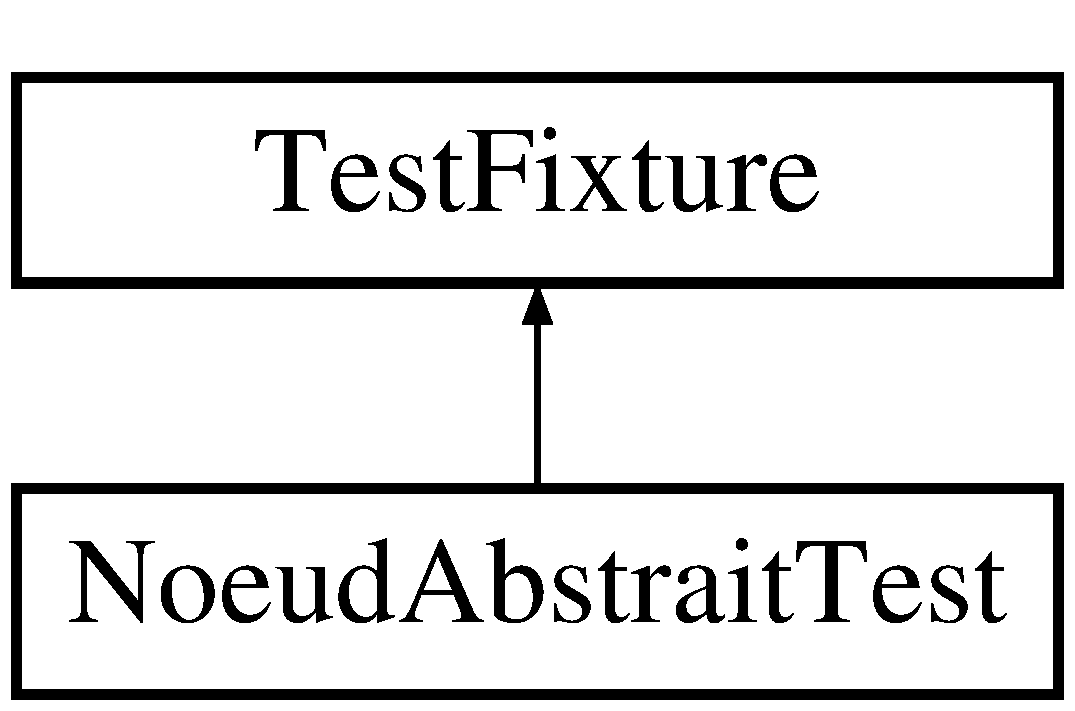
\includegraphics[height=2.000000cm]{class_noeud_abstrait_test}
\end{center}
\end{figure}
\subsection*{Public Member Functions}
\begin{DoxyCompactItemize}
\item 
void \hyperlink{group__inf2990_ga4d2fe388f550ba374823d09b5c8ebe77}{set\+Up} ()
\begin{DoxyCompactList}\small\item\em Traitement � effectuer pour initialiser cette suite de tests. \end{DoxyCompactList}\item 
void \hyperlink{group__inf2990_ga2c5c558ff7e40386c724a55b670af417}{tear\+Down} ()
\begin{DoxyCompactList}\small\item\em Traitement � effectuer pour \textquotesingle{}finaliser\textquotesingle{} cette suite de tests. \end{DoxyCompactList}\item 
void \hyperlink{group__inf2990_gaed7a5423d2a3a7518aef743f17d32ccd}{test\+Position\+Relative} ()
\begin{DoxyCompactList}\small\item\em Cas de test\+: �criture/lecture de la position relative. \end{DoxyCompactList}\item 
void \hyperlink{group__inf2990_gadf554a62266cc21c7c48f6a27ad7c752}{test\+Type} ()
\begin{DoxyCompactList}\small\item\em Cas de test\+: type de noeud. \end{DoxyCompactList}\item 
void \hyperlink{group__inf2990_gac044744b04574c86418a57b39e3238ff}{test\+Selection} ()
\begin{DoxyCompactList}\small\item\em Cas de test\+: d�finition/obtention des �tats de s�lection du noeud. \end{DoxyCompactList}\item 
void \hyperlink{group__inf2990_ga0e65b00620e79646a9efd8a93c4fc650}{test\+Enfants} ()
\begin{DoxyCompactList}\small\item\em Cas de test\+: s\textquotesingle{}assurer que le noeud abstrait n\textquotesingle{}a pas d\textquotesingle{}enfant. \end{DoxyCompactList}\end{DoxyCompactItemize}


\subsection{Detailed Description}
Classe de test cppunit pour tester le bon fonctionnement des m�thodes de la classe \hyperlink{class_noeud_abstrait}{Noeud\+Abstrait}. 

\begin{DoxyAuthor}{Author}
Julien Gascon-\/\+Samson 
\end{DoxyAuthor}
\begin{DoxyDate}{Date}
2011-\/07-\/16 
\end{DoxyDate}


The documentation for this class was generated from the following files\+:\begin{DoxyCompactItemize}
\item 
Sources/\+D\+L\+L/\+Tests/\hyperlink{_noeud_abstrait_test_8h}{Noeud\+Abstrait\+Test.\+h}\item 
Sources/\+D\+L\+L/\+Tests/\hyperlink{_noeud_abstrait_test_8cpp}{Noeud\+Abstrait\+Test.\+cpp}\end{DoxyCompactItemize}

\hypertarget{class_noeud_araignee}{}\section{Noeud\+Araignee Class Reference}
\label{class_noeud_araignee}\index{Noeud\+Araignee@{Noeud\+Araignee}}


Classe qui repr�sente un exemple de noeud de l\textquotesingle{}arbre de rendu.  




{\ttfamily \#include $<$Noeud\+Araignee.\+h$>$}

Inheritance diagram for Noeud\+Araignee\+:\begin{figure}[H]
\begin{center}
\leavevmode
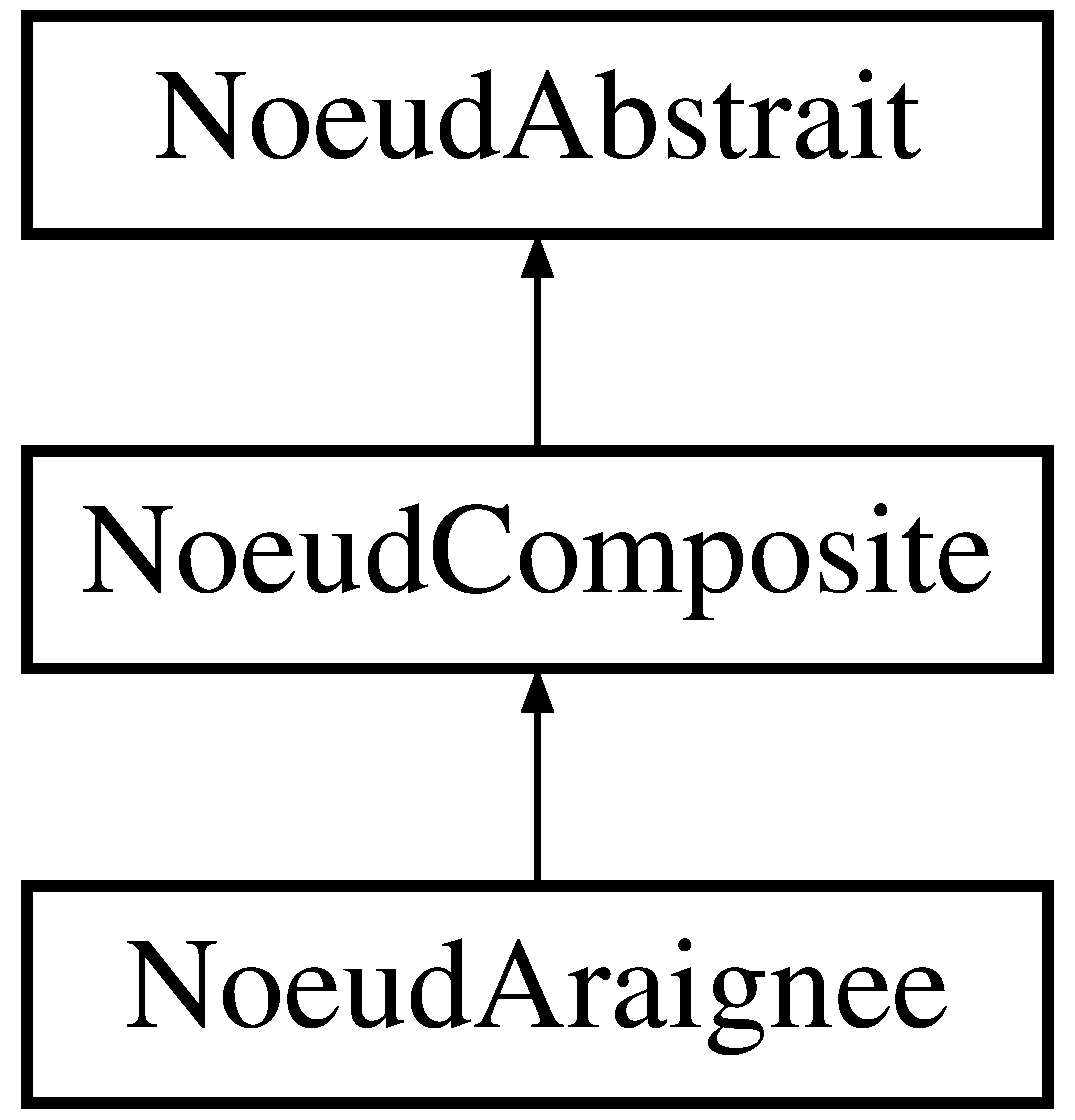
\includegraphics[height=3.000000cm]{class_noeud_araignee}
\end{center}
\end{figure}
\subsection*{Public Member Functions}
\begin{DoxyCompactItemize}
\item 
\hyperlink{group__inf2990_ga0ca3d14d5baf9c6879ac53918cc54ba5}{Noeud\+Araignee} (const std\+::string \&type\+Noeud)
\begin{DoxyCompactList}\small\item\em Constructeur � partir du type du noeud. \end{DoxyCompactList}\item 
\hyperlink{group__inf2990_ga78bf0250c601da26edb8cd8f2cddec10}{$\sim$\+Noeud\+Araignee} ()
\begin{DoxyCompactList}\small\item\em Destructeur. \end{DoxyCompactList}\item 
virtual void \hyperlink{group__inf2990_ga9602465d8095ce3a306b6644e5476171}{afficher\+Concret} (const glm\+::mat4 \&vue\+Projection) const
\begin{DoxyCompactList}\small\item\em Affiche le cube. \end{DoxyCompactList}\item 
virtual void \hyperlink{group__inf2990_gae3f4c490330d597a18975014c06a05ca}{animer} (float temps)
\begin{DoxyCompactList}\small\item\em Effectue l\textquotesingle{}animation du cube. \end{DoxyCompactList}\end{DoxyCompactItemize}
\subsection*{Additional Inherited Members}


\subsection{Detailed Description}
Classe qui repr�sente un exemple de noeud de l\textquotesingle{}arbre de rendu. 

\begin{DoxyAuthor}{Author}
Julien Gascon-\/\+Samson 
\end{DoxyAuthor}
\begin{DoxyDate}{Date}
2011-\/05-\/19 
\end{DoxyDate}


The documentation for this class was generated from the following files\+:\begin{DoxyCompactItemize}
\item 
Sources/\+D\+L\+L/\+Arbre/\+Noeuds/\hyperlink{_noeud_araignee_8h}{Noeud\+Araignee.\+h}\item 
Sources/\+D\+L\+L/\+Arbre/\+Noeuds/\hyperlink{_noeud_araignee_8cpp}{Noeud\+Araignee.\+cpp}\item 
Sources/\+D\+L\+L/\+Arbre/\+Noeuds/Noeud\+Rondelle.\+cpp\end{DoxyCompactItemize}

\hypertarget{class_noeud_bonus_accelerateur}{}\section{Noeud\+Bonus\+Accelerateur Class Reference}
\label{class_noeud_bonus_accelerateur}\index{Noeud\+Bonus\+Accelerateur@{Noeud\+Bonus\+Accelerateur}}


Classe qui repr�sente un exemple de noeud de l\textquotesingle{}arbre de rendu.  




{\ttfamily \#include $<$Noeud\+Bonus\+Accelerateur.\+h$>$}

Inheritance diagram for Noeud\+Bonus\+Accelerateur\+:\begin{figure}[H]
\begin{center}
\leavevmode
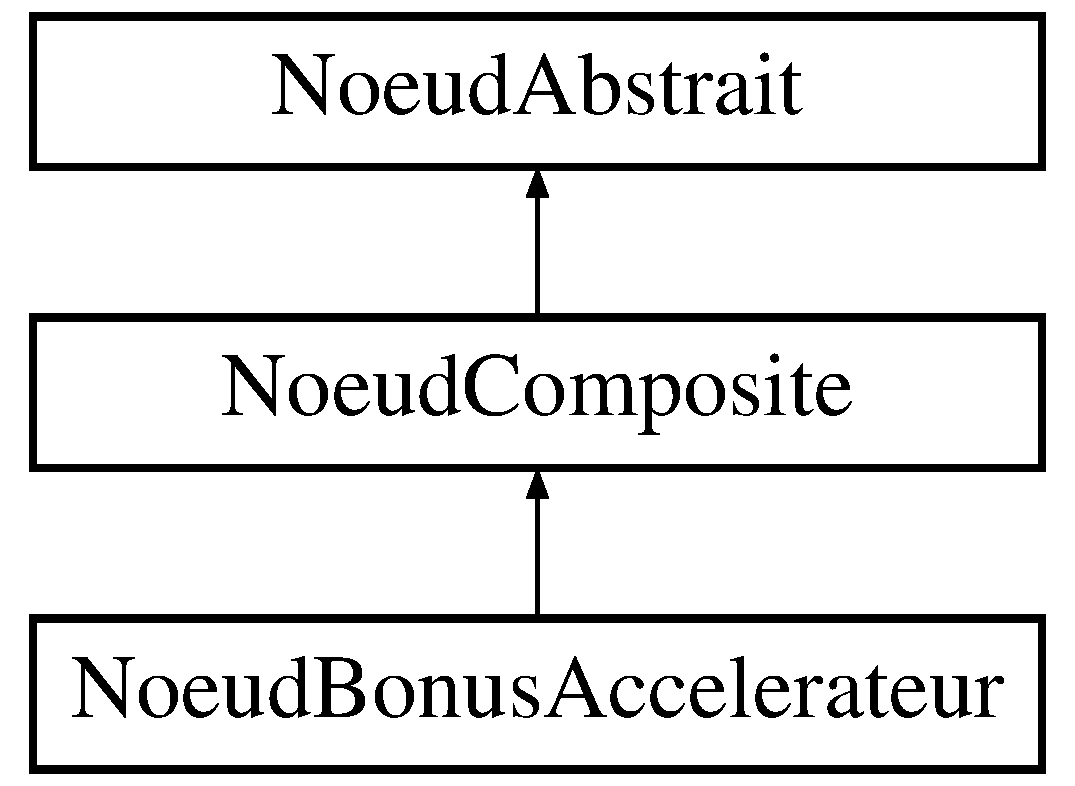
\includegraphics[height=3.000000cm]{class_noeud_bonus_accelerateur}
\end{center}
\end{figure}
\subsection*{Public Member Functions}
\begin{DoxyCompactItemize}
\item 
\hyperlink{group__inf2990_ga4af18e0215e621cf95d4611a1c5f09c8}{Noeud\+Bonus\+Accelerateur} (const std\+::string \&type\+Noeud)
\begin{DoxyCompactList}\small\item\em Constructeur � partir du type du noeud. \end{DoxyCompactList}\item 
\hyperlink{group__inf2990_ga0675ba182334b41d9c11092b34fa0e99}{$\sim$\+Noeud\+Bonus\+Accelerateur} ()
\begin{DoxyCompactList}\small\item\em Destructeur. \end{DoxyCompactList}\item 
void {\bfseries copier\+Attributs} (\hyperlink{class_noeud_bonus_accelerateur}{Noeud\+Bonus\+Accelerateur} \&destination)
\item 
virtual void \hyperlink{group__inf2990_gab6b2529d8c37ef9f1b972c486072fdcb}{afficher\+Concret} (const glm\+::mat4 \&vue\+Projection, const bool \&attribuer\+Couleur) const
\begin{DoxyCompactList}\small\item\em Affiche le cube. \end{DoxyCompactList}\item 
virtual void \hyperlink{group__inf2990_ga31899d28a0c6afb0c29bbf3503218323}{animer} (float temps)
\begin{DoxyCompactList}\small\item\em Effectue l\textquotesingle{}animation du cube. \end{DoxyCompactList}\item 
void \hyperlink{group__inf2990_ga03570ae76f98c52bd9ebb9d8b6753d69}{accepter\+Visiteur} (\hyperlink{class_visiteur_abstrait}{Visiteur\+Abstrait} $\ast$visiteur)
\item 
bool \hyperlink{group__inf2990_ga9e2093ef97c7485f6c5899de71f49fe9}{verifier\+Selection} (G\+Lubyte couleur\+Objet\mbox{[}$\,$\mbox{]})
\end{DoxyCompactItemize}
\subsection*{Additional Inherited Members}


\subsection{Detailed Description}
Classe qui repr�sente un exemple de noeud de l\textquotesingle{}arbre de rendu. 

\begin{DoxyAuthor}{Author}
Equipe06 
\end{DoxyAuthor}
\begin{DoxyDate}{Date}
2016-\/09-\/07 
\end{DoxyDate}


The documentation for this class was generated from the following files\+:\begin{DoxyCompactItemize}
\item 
Sources/\+D\+L\+L/\+Arbre/\+Noeuds/\hyperlink{_noeud_bonus_accelerateur_8h}{Noeud\+Bonus\+Accelerateur.\+h}\item 
Sources/\+D\+L\+L/\+Arbre/\+Noeuds/Noeud\+Bonus\+Accelerateur.\+cpp\end{DoxyCompactItemize}

\hypertarget{class_noeud_cercle}{}\section{Noeud\+Cercle Class Reference}
\label{class_noeud_cercle}\index{Noeud\+Cercle@{Noeud\+Cercle}}
Inheritance diagram for Noeud\+Cercle\+:\begin{figure}[H]
\begin{center}
\leavevmode
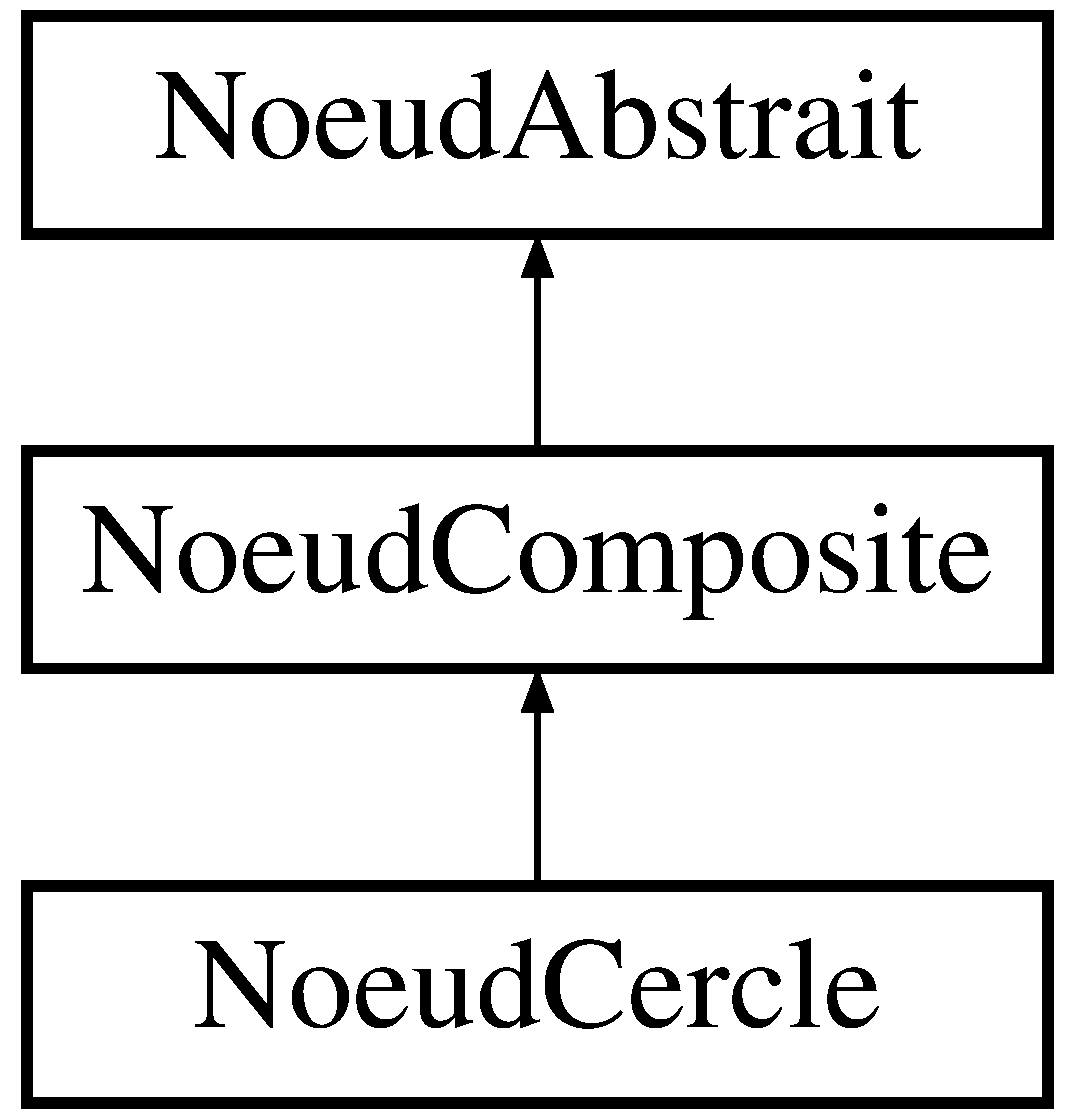
\includegraphics[height=3.000000cm]{class_noeud_cercle}
\end{center}
\end{figure}
\subsection*{Public Member Functions}
\begin{DoxyCompactItemize}
\item 
\hyperlink{group__inf2990_ga3f811397073ca10d6657425c0a45f17a}{Noeud\+Cercle} (const std\+::string \&type\+Noeud)
\begin{DoxyCompactList}\small\item\em Constructeur � partir du type du noeud. \end{DoxyCompactList}\item 
\hyperlink{group__inf2990_gafe4f3c643fd10c9fc92b777ffadc970d}{$\sim$\+Noeud\+Cercle} ()
\begin{DoxyCompactList}\small\item\em Destructeur. \end{DoxyCompactList}\item 
void {\bfseries copier\+Attributs} (\hyperlink{class_noeud_cercle}{Noeud\+Cercle} \&destination)
\item 
virtual void \hyperlink{group__inf2990_ga8e2d266cad420ccd4fd305d9d296b2b5}{afficher\+Concret} (const glm\+::mat4 \&vue\+Projection, const bool \&attribuer\+Couleur) const
\begin{DoxyCompactList}\small\item\em Affiche le cube. \end{DoxyCompactList}\item 
virtual void \hyperlink{group__inf2990_gaa53138aa3aeaefc88e47a94d3e7ab811}{animer} (float temps)
\begin{DoxyCompactList}\small\item\em Effectue l\textquotesingle{}animation du cube. \end{DoxyCompactList}\item 
void \hyperlink{group__inf2990_gaf012e22b8b62a49e8ea88b369ec4478e}{accepter\+Visiteur} (\hyperlink{class_visiteur_abstrait}{Visiteur\+Abstrait} $\ast$visiteur)
\item 
virtual bool \hyperlink{group__inf2990_ga6cae68c636fb6bf5be6b969593380b6f}{est\+Dans\+La\+Table} ()
\begin{DoxyCompactList}\small\item\em permet de verifier si un objet est toujours a l\textquotesingle{}interieur de la table. \end{DoxyCompactList}\item 
virtual void {\bfseries redefinir\+Sommets} ()
\item 
void \hyperlink{group__inf2990_gace82bbff0df7954c24d8c7b16181c04c}{assigner\+Objet\+Rendu} (modele\+::\+Modele3D const $\ast$modele, opengl\+::\+V\+BO const $\ast$liste) override
\begin{DoxyCompactList}\small\item\em Assigne le mod�le3D et la liste d\textquotesingle{}affichage du noeud courant. \end{DoxyCompactList}\end{DoxyCompactItemize}
\subsection*{Additional Inherited Members}


The documentation for this class was generated from the following files\+:\begin{DoxyCompactItemize}
\item 
C\+:/\+Users/\+Steven/\+Documents/\+Poly/\+I\+N\+F2990/inf2990-\/06/\+Cadriciel\+\_\+2016-\/3\+\_\+\+Etudiants/\+Cadriciel/\+Sources/\+D\+L\+L/\+Arbre/\+Noeuds/Noeud\+Cercle.\+h\item 
C\+:/\+Users/\+Steven/\+Documents/\+Poly/\+I\+N\+F2990/inf2990-\/06/\+Cadriciel\+\_\+2016-\/3\+\_\+\+Etudiants/\+Cadriciel/\+Sources/\+D\+L\+L/\+Arbre/\+Noeuds/Noeud\+Cercle.\+cpp\end{DoxyCompactItemize}

\hypertarget{class_noeud_composite}{}\section{Noeud\+Composite Class Reference}
\label{class_noeud_composite}\index{Noeud\+Composite@{Noeud\+Composite}}


Implantation d\textquotesingle{}un noeud du patron composite qui peut poss�der des enfants.  




{\ttfamily \#include $<$Noeud\+Composite.\+h$>$}

Inheritance diagram for Noeud\+Composite\+:\begin{figure}[H]
\begin{center}
\leavevmode
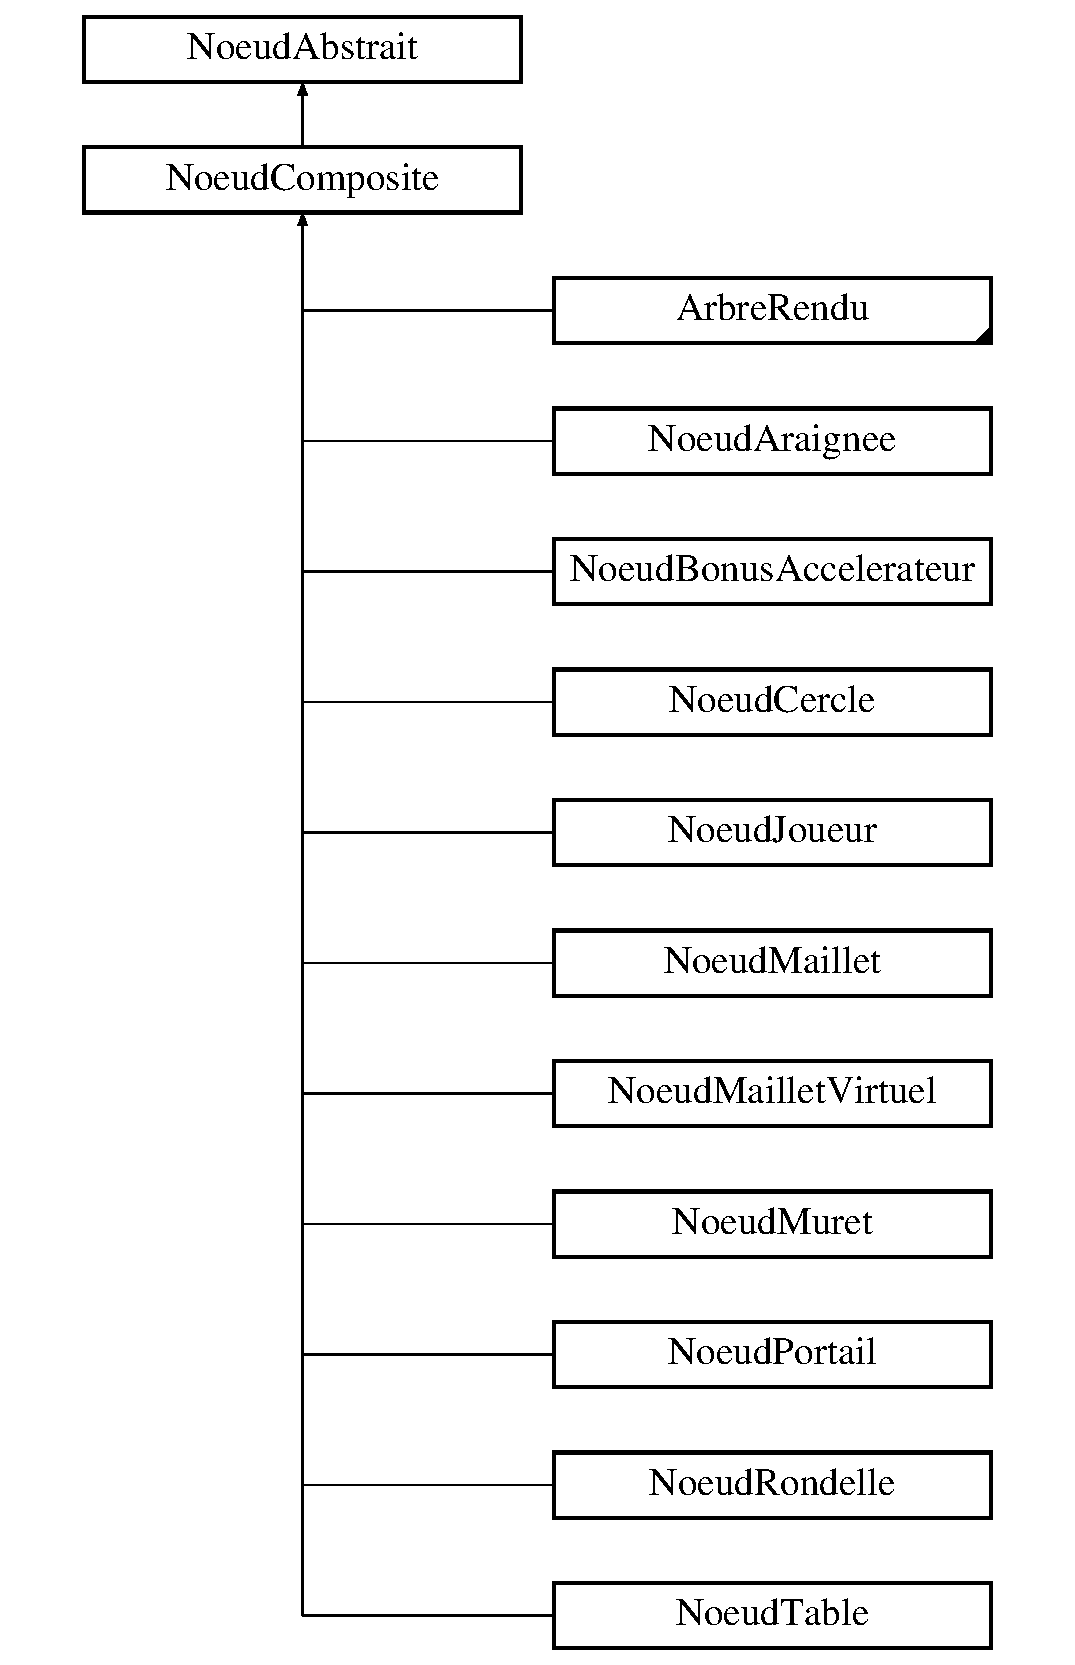
\includegraphics[height=12.000000cm]{class_noeud_composite}
\end{center}
\end{figure}
\subsection*{Public Member Functions}
\begin{DoxyCompactItemize}
\item 
\hyperlink{group__inf2990_ga232a795d9c9fca9996e4fc6b05a0f01e}{Noeud\+Composite} (const std\+::string \&type=std\+::string\{ \char`\"{}\char`\"{} \})
\begin{DoxyCompactList}\small\item\em Constructeur. \end{DoxyCompactList}\item 
virtual \hyperlink{group__inf2990_gaada4bd846bd950f2ac186b09f35aa9c6}{$\sim$\+Noeud\+Composite} ()
\begin{DoxyCompactList}\small\item\em Destructeur. \end{DoxyCompactList}\item 
virtual unsigned int \hyperlink{group__inf2990_gaf9dcb057d20a02985775c7797a2ad788}{calculer\+Profondeur} () const
\begin{DoxyCompactList}\small\item\em Calcule la profondeur de l\textquotesingle{}arbre sous le noeud courant. \end{DoxyCompactList}\item 
virtual void \hyperlink{group__inf2990_ga5e1564f2f07f5cd84cef7078ae88e3c6}{vider} ()
\begin{DoxyCompactList}\small\item\em Vide le noeud de ses enfants. \end{DoxyCompactList}\item 
virtual void \hyperlink{group__inf2990_gabdc10574cb2b5c4825bc10b610fa9b5d}{effacer} (const \hyperlink{class_noeud_abstrait}{Noeud\+Abstrait} $\ast$noeud)
\begin{DoxyCompactList}\small\item\em Efface le noeud pass� en param�tre. \end{DoxyCompactList}\item 
virtual const \hyperlink{class_noeud_abstrait}{Noeud\+Abstrait} $\ast$ \hyperlink{group__inf2990_ga6dc1e08f5898defb3d25b4167b20759c}{chercher} (const std\+::string \&type\+Noeud) const
\begin{DoxyCompactList}\small\item\em Cherche un noeud par le type (sur un noeud constant). \end{DoxyCompactList}\item 
virtual \hyperlink{class_noeud_abstrait}{Noeud\+Abstrait} $\ast$ \hyperlink{group__inf2990_ga622dcce31cdfb05afeedb7602e007f25}{chercher} (const std\+::string \&type\+Noeud)
\begin{DoxyCompactList}\small\item\em Cherche un noeud par le type. \end{DoxyCompactList}\item 
virtual const \hyperlink{class_noeud_abstrait}{Noeud\+Abstrait} $\ast$ \hyperlink{group__inf2990_gaa904962f12f72ee257a442fc376fe99e}{chercher} (unsigned int indice) const
\begin{DoxyCompactList}\small\item\em Cherche un noeud enfant selon l\textquotesingle{}indice (sur un noeud constant). \end{DoxyCompactList}\item 
virtual \hyperlink{class_noeud_abstrait}{Noeud\+Abstrait} $\ast$ \hyperlink{group__inf2990_ga67f24432c3a667154adf005f2c6c4396}{chercher} (unsigned int indice)
\begin{DoxyCompactList}\small\item\em Cherche un noeud enfant selon l\textquotesingle{}indice. \end{DoxyCompactList}\item 
virtual bool \hyperlink{group__inf2990_gac2ce823d2c52140d4e1a924163ebbb58}{ajouter} (\hyperlink{class_noeud_abstrait}{Noeud\+Abstrait} $\ast$enfant)
\begin{DoxyCompactList}\small\item\em Ajoute un noeud enfant. \end{DoxyCompactList}\item 
virtual unsigned int \hyperlink{group__inf2990_gaec16f4b7c2b7888821de434a482df586}{obtenir\+Nombre\+Enfants} () const
\begin{DoxyCompactList}\small\item\em Obtient le nombre d\textquotesingle{}enfants du noeud. \end{DoxyCompactList}\item 
virtual void \hyperlink{group__inf2990_ga64bcef79a467ea669275d885dbe31c8d}{effacer\+Selection} ()
\begin{DoxyCompactList}\small\item\em Efface les enfants s�lectionn�s. \end{DoxyCompactList}\item 
virtual void \hyperlink{group__inf2990_ga6c0620784aa50cb5c19664124e884cdd}{selectionner\+Tout} ()
\begin{DoxyCompactList}\small\item\em S�lectionne tous les enfants de m�me que le noeud. \end{DoxyCompactList}\item 
virtual void \hyperlink{group__inf2990_ga0a838e8f0a086e71856e3a116508bcf2}{deselectionner\+Tout} ()
\begin{DoxyCompactList}\small\item\em D�s�lectionne tous les enfants de m�me que le noeud. \end{DoxyCompactList}\item 
virtual bool \hyperlink{group__inf2990_ga2eac267d84a067ff59f64319c98d872e}{selection\+Existe} () const
\begin{DoxyCompactList}\small\item\em V�rifier si le noeud ou un de ses enfants est s�lectionn�. \end{DoxyCompactList}\item 
virtual void \hyperlink{group__inf2990_ga106605948d7ae3ba99d9d9df83a0dbc2}{selectionner\+Objets} (int x, int y, int hauteur, int largeur, bool etat\+C\+T\+RL, bool selection\+Unique)
\begin{DoxyCompactList}\small\item\em fonction qui effectue la selection propre \end{DoxyCompactList}\item 
int \hyperlink{group__inf2990_ga5723387234ad51dd0b6b1fe012e735be}{calculer\+Nombre\+Selectionner} () const
\begin{DoxyCompactList}\small\item\em Calcul du nombre d\textquotesingle{}enfants selectionner. \end{DoxyCompactList}\item 
virtual void \hyperlink{group__inf2990_gafcbaa01f832fc2dad13b363253963d0b}{changer\+Mode\+Polygones} (bool est\+Force)
\begin{DoxyCompactList}\small\item\em Change le mode d\textquotesingle{}affichage des polygones. \end{DoxyCompactList}\item 
virtual void \hyperlink{group__inf2990_gaeeeca055ef6aef0435b9956eb467ff7f}{assigner\+Mode\+Polygones} (G\+Lenum mode\+Polygones)
\begin{DoxyCompactList}\small\item\em Assigne le mode d\textquotesingle{}affichage des polygones. \end{DoxyCompactList}\item 
virtual void \hyperlink{group__inf2990_gac395ac1bbd34bcf4fe38b2b09b97ab03}{afficher\+Concret} (const glm\+::mat4 \&vue\+Projection, const bool \&attribuer\+Couleur) const
\begin{DoxyCompactList}\small\item\em Affiche le noeud de mani�re concr�te. \end{DoxyCompactList}\item 
virtual void \hyperlink{group__inf2990_ga57f31e1a0fd79628d04651001014fd41}{animer} (float dt)
\begin{DoxyCompactList}\small\item\em Anime le noeud. \end{DoxyCompactList}\item 
virtual void {\bfseries redessiner} ()
\item 
virtual \hyperlink{group__inf2990_gae5f081f07546f0b622ee841a2d6e5a0d}{conteneur\+\_\+enfants} \hyperlink{group__inf2990_ga7b92102e65b3d0207902a510d4bcab4a}{obtenir\+Enfants} ()
\begin{DoxyCompactList}\small\item\em verifier si la noeud est dans la table \end{DoxyCompactList}\item 
void \hyperlink{group__inf2990_gabba8d47a97ed051b25bc842f080ecabc}{attribuer\+Couleur\+Selection} ()
\item 
void \hyperlink{group__inf2990_ga085a36a9c2f9e767ec1229c900b300ab}{accepter\+Visiteur} (\hyperlink{class_visiteur_abstrait}{Visiteur\+Abstrait} $\ast$visiteur, bool select)
\end{DoxyCompactItemize}
\subsection*{Protected Attributes}
\begin{DoxyCompactItemize}
\item 
\hypertarget{class_noeud_composite_a628227fd324020e497ada7577457ff3f}{}\label{class_noeud_composite_a628227fd324020e497ada7577457ff3f} 
\hyperlink{group__inf2990_gae5f081f07546f0b622ee841a2d6e5a0d}{conteneur\+\_\+enfants} \hyperlink{class_noeud_composite_a628227fd324020e497ada7577457ff3f}{enfants\+\_\+}
\begin{DoxyCompactList}\small\item\em La liste des enfants. \end{DoxyCompactList}\end{DoxyCompactItemize}
\subsection*{Additional Inherited Members}


\subsection{Detailed Description}
Implantation d\textquotesingle{}un noeud du patron composite qui peut poss�der des enfants. 

Cette classe implante les diff�rentes fonctions relatives aux enfants, comme l\textquotesingle{}ajout, le retrait, la recherche, etc.

\begin{DoxyAuthor}{Author}
D\+G\+I-\/2990 
\end{DoxyAuthor}
\begin{DoxyDate}{Date}
2007-\/01-\/24 
\end{DoxyDate}


The documentation for this class was generated from the following files\+:\begin{DoxyCompactItemize}
\item 
Sources/\+D\+L\+L/\+Arbre/\+Noeuds/\hyperlink{_noeud_composite_8h}{Noeud\+Composite.\+h}\item 
Sources/\+D\+L\+L/\+Arbre/\+Noeuds/\hyperlink{_noeud_composite_8cpp}{Noeud\+Composite.\+cpp}\end{DoxyCompactItemize}

\hypertarget{class_noeud_cone_cube}{}\section{Noeud\+Cone\+Cube Class Reference}
\label{class_noeud_cone_cube}\index{Noeud\+Cone\+Cube@{Noeud\+Cone\+Cube}}


Classe qui repr�sente un exemple de noeud de l\textquotesingle{}arbre de rendu.  




{\ttfamily \#include $<$Noeud\+Cone\+Cube.\+h$>$}

Inheritance diagram for Noeud\+Cone\+Cube\+:\begin{figure}[H]
\begin{center}
\leavevmode
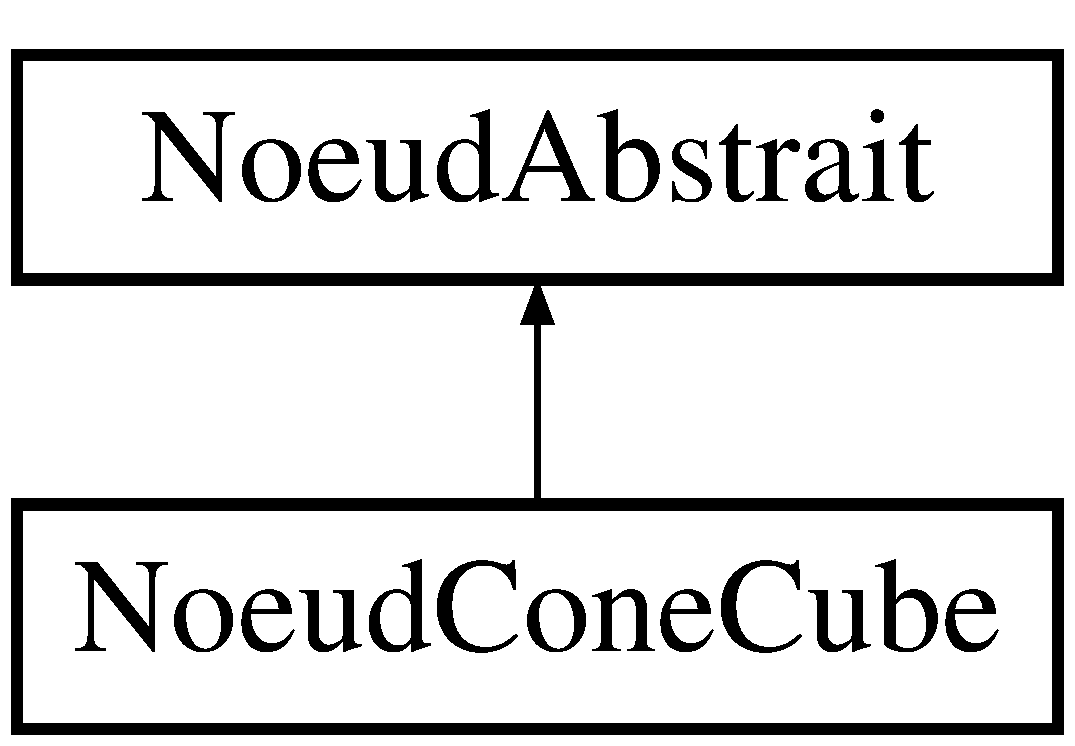
\includegraphics[height=2.000000cm]{class_noeud_cone_cube}
\end{center}
\end{figure}
\subsection*{Public Member Functions}
\begin{DoxyCompactItemize}
\item 
\hyperlink{group__inf2990_ga6f0bcd8b494e8aa6f3a8dad78bad2c0f}{Noeud\+Cone\+Cube} (const std\+::string \&type\+Noeud)
\begin{DoxyCompactList}\small\item\em Constructeur � partir du type du noeud. \end{DoxyCompactList}\item 
\hyperlink{group__inf2990_ga8db4b36c3469001f7dcfab23debe7d2f}{$\sim$\+Noeud\+Cone\+Cube} ()
\begin{DoxyCompactList}\small\item\em Destructeur. \end{DoxyCompactList}\item 
virtual void \hyperlink{group__inf2990_gabd3cd73691f5760369ad5ef68957a49b}{afficher\+Concret} (const glm\+::mat4 \&vue\+Projection) const
\begin{DoxyCompactList}\small\item\em Affiche le cube. \end{DoxyCompactList}\item 
virtual void \hyperlink{group__inf2990_ga3472a200d45ce3cdff72d72921807b21}{animer} (float temps)
\begin{DoxyCompactList}\small\item\em Effectue l\textquotesingle{}animation du cube. \end{DoxyCompactList}\end{DoxyCompactItemize}
\subsection*{Additional Inherited Members}


\subsection{Detailed Description}
Classe qui repr�sente un exemple de noeud de l\textquotesingle{}arbre de rendu. 

\begin{DoxyAuthor}{Author}
Julien Gascon-\/\+Samson 
\end{DoxyAuthor}
\begin{DoxyDate}{Date}
2011-\/05-\/19 
\end{DoxyDate}


The documentation for this class was generated from the following files\+:\begin{DoxyCompactItemize}
\item 
C\+:/\+Users/\+Steven/\+Documents/\+Poly/\+I\+N\+F2990/inf2990-\/06/\+Cadriciel\+\_\+2016-\/3\+\_\+\+Etudiants/\+Cadriciel/\+Sources/\+D\+L\+L/\+Arbre/\+Noeuds/\hyperlink{_noeud_cone_cube_8h}{Noeud\+Cone\+Cube.\+h}\item 
C\+:/\+Users/\+Steven/\+Documents/\+Poly/\+I\+N\+F2990/inf2990-\/06/\+Cadriciel\+\_\+2016-\/3\+\_\+\+Etudiants/\+Cadriciel/\+Sources/\+D\+L\+L/\+Arbre/\+Noeuds/\hyperlink{_noeud_cone_cube_8cpp}{Noeud\+Cone\+Cube.\+cpp}\end{DoxyCompactItemize}

\hypertarget{class_noeud_joueur}{}\section{Noeud\+Joueur Class Reference}
\label{class_noeud_joueur}\index{Noeud\+Joueur@{Noeud\+Joueur}}
Inheritance diagram for Noeud\+Joueur\+:\begin{figure}[H]
\begin{center}
\leavevmode
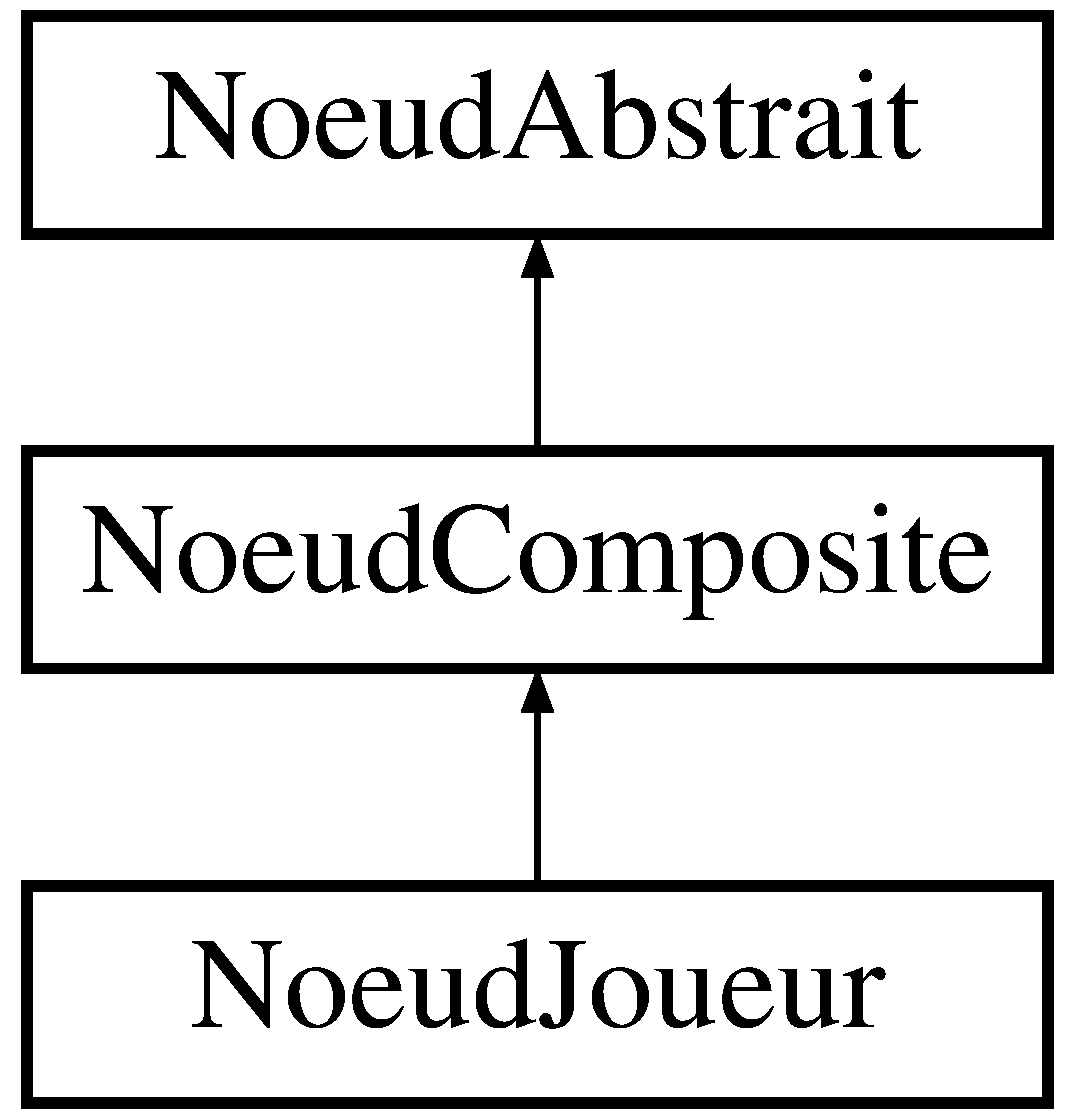
\includegraphics[height=3.000000cm]{class_noeud_joueur}
\end{center}
\end{figure}
\subsection*{Public Member Functions}
\begin{DoxyCompactItemize}
\item 
\hypertarget{class_noeud_joueur_a39839234b97274cf4c9b3a16bc0881b8}{}\label{class_noeud_joueur_a39839234b97274cf4c9b3a16bc0881b8} 
\hyperlink{class_noeud_joueur_a39839234b97274cf4c9b3a16bc0881b8}{Noeud\+Joueur} ()
\begin{DoxyCompactList}\small\item\em Constructeur � partir du type du noeud. \end{DoxyCompactList}\item 
\hypertarget{class_noeud_joueur_a46f084aba4e5e599c9612254f8c34682}{}\label{class_noeud_joueur_a46f084aba4e5e599c9612254f8c34682} 
{\bfseries Noeud\+Joueur} (bool virtuel, std\+::string nom)
\item 
\hypertarget{class_noeud_joueur_aaf32ca98814fd016251c240d07d87e69}{}\label{class_noeud_joueur_aaf32ca98814fd016251c240d07d87e69} 
virtual \hyperlink{class_noeud_joueur_aaf32ca98814fd016251c240d07d87e69}{$\sim$\+Noeud\+Joueur} ()
\begin{DoxyCompactList}\small\item\em Destructeur. \end{DoxyCompactList}\item 
\hypertarget{class_noeud_joueur_a48b64269e804787f12c21bb37bb496d8}{}\label{class_noeud_joueur_a48b64269e804787f12c21bb37bb496d8} 
void {\bfseries assigner\+Maillet} (\hyperlink{class_noeud_abstrait}{Noeud\+Abstrait} $\ast$node)
\item 
\hypertarget{class_noeud_joueur_a98442b6162127637374cedcd4918dcd7}{}\label{class_noeud_joueur_a98442b6162127637374cedcd4918dcd7} 
int {\bfseries get\+But} () const
\item 
\hypertarget{class_noeud_joueur_a76ad18f363c6ca8184ad1e1dd55cff11}{}\label{class_noeud_joueur_a76ad18f363c6ca8184ad1e1dd55cff11} 
\hyperlink{class_noeud_abstrait}{Noeud\+Abstrait} $\ast$ {\bfseries get\+Maillet} ()
\item 
\hypertarget{class_noeud_joueur_aa4c60c7c8a8e1aeea393e9ddf7cf3a16}{}\label{class_noeud_joueur_aa4c60c7c8a8e1aeea393e9ddf7cf3a16} 
\hyperlink{class_noeud_maillet_virtuel}{Noeud\+Maillet\+Virtuel} $\ast$ {\bfseries get\+Maillet\+Virtuel} ()
\item 
\hypertarget{class_noeud_joueur_af797506a84c6a188f1af969b85ead852}{}\label{class_noeud_joueur_af797506a84c6a188f1af969b85ead852} 
void {\bfseries incrementer\+But} ()
\item 
\hypertarget{class_noeud_joueur_ae8b99a29da69924b493627497f36632a}{}\label{class_noeud_joueur_ae8b99a29da69924b493627497f36632a} 
void {\bfseries reinitialiser\+But} ()
\item 
\hypertarget{class_noeud_joueur_ad675b73b7d7c6a57a61693f474a759ce}{}\label{class_noeud_joueur_ad675b73b7d7c6a57a61693f474a759ce} 
void {\bfseries set\+But} (int)
\item 
\hypertarget{class_noeud_joueur_ac3d505b849a21bbe55cfeeb89b11aab9}{}\label{class_noeud_joueur_ac3d505b849a21bbe55cfeeb89b11aab9} 
bool {\bfseries est\+Virtuel} ()
\item 
\hypertarget{class_noeud_joueur_a1b7b668fdd7dc4a127e2d13d218e4d68}{}\label{class_noeud_joueur_a1b7b668fdd7dc4a127e2d13d218e4d68} 
void {\bfseries set\+Virtuel} (bool virtuel)
\item 
\hypertarget{class_noeud_joueur_a343fdf854cd00935298f2a9d56e881a6}{}\label{class_noeud_joueur_a343fdf854cd00935298f2a9d56e881a6} 
void {\bfseries assigner\+Nom} (std\+::string nom)
\item 
\hypertarget{class_noeud_joueur_a516b71a2db6659a3d94e465daa92cbd3}{}\label{class_noeud_joueur_a516b71a2db6659a3d94e465daa92cbd3} 
std\+::string {\bfseries get\+Nom} ()
\end{DoxyCompactItemize}
\subsection*{Additional Inherited Members}


The documentation for this class was generated from the following files\+:\begin{DoxyCompactItemize}
\item 
C\+:/\+Users/\+Steven/\+Documents/\+Poly/\+I\+N\+F2990/inf2990-\/06/\+Cadriciel\+\_\+2016-\/3\+\_\+\+Etudiants/\+Cadriciel/\+Sources/\+D\+L\+L/\+Arbre/\+Noeuds/Noeud\+Joueur.\+h\item 
C\+:/\+Users/\+Steven/\+Documents/\+Poly/\+I\+N\+F2990/inf2990-\/06/\+Cadriciel\+\_\+2016-\/3\+\_\+\+Etudiants/\+Cadriciel/\+Sources/\+D\+L\+L/\+Arbre/\+Noeuds/\hyperlink{_noeud_joueur_8cpp}{Noeud\+Joueur.\+cpp}\end{DoxyCompactItemize}

\hypertarget{class_noeud_maillet}{}\section{Noeud\+Maillet Class Reference}
\label{class_noeud_maillet}\index{Noeud\+Maillet@{Noeud\+Maillet}}


Classe qui repr�sente un exemple de noeud de l\textquotesingle{}arbre de rendu.  




{\ttfamily \#include $<$Noeud\+Maillet.\+h$>$}

Inheritance diagram for Noeud\+Maillet\+:\begin{figure}[H]
\begin{center}
\leavevmode
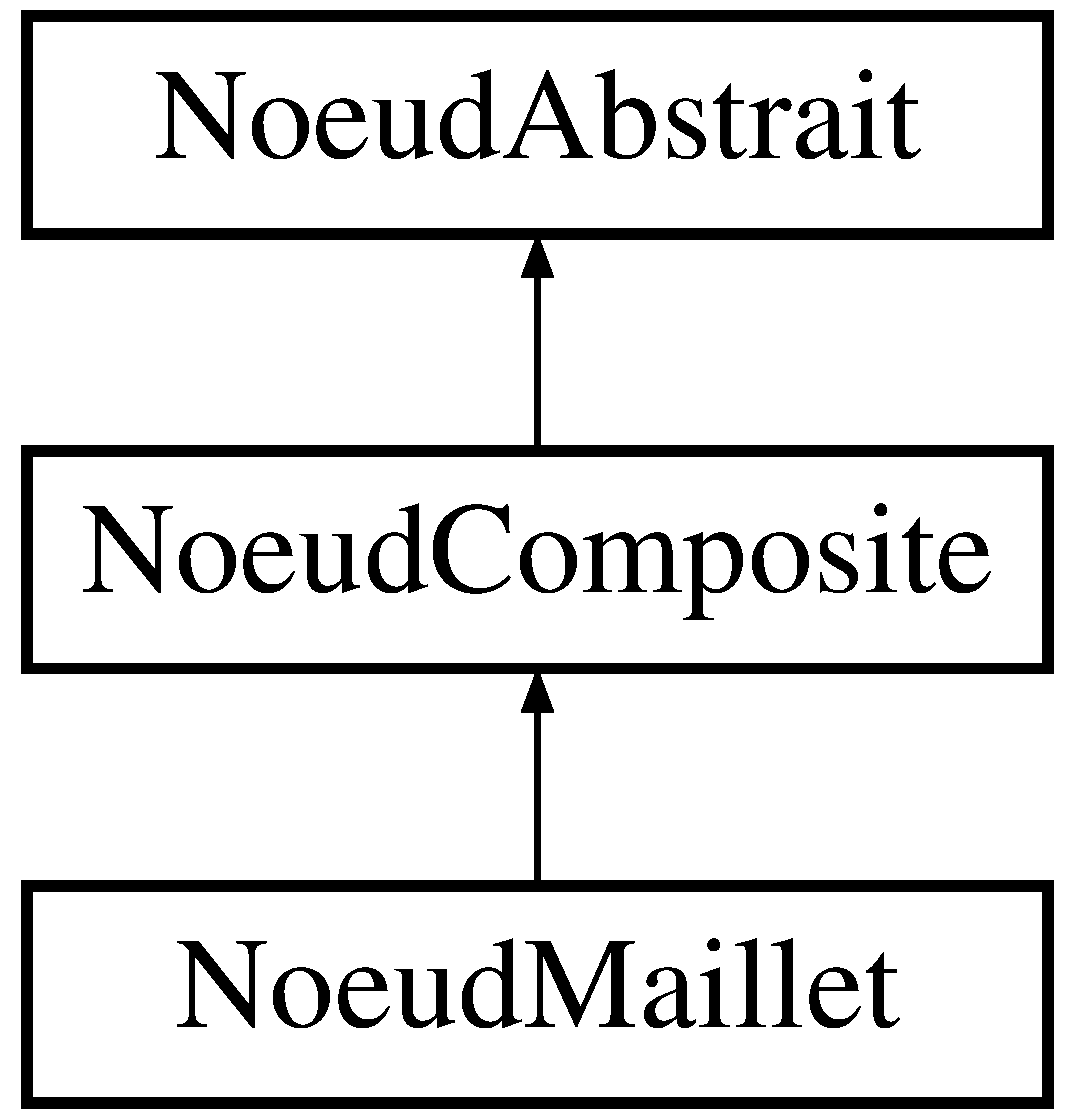
\includegraphics[height=3.000000cm]{class_noeud_maillet}
\end{center}
\end{figure}
\subsection*{Public Member Functions}
\begin{DoxyCompactItemize}
\item 
\hyperlink{group__inf2990_ga70af0f07ba3a81cca52a11a06544690e}{Noeud\+Maillet} (const std\+::string \&type\+Noeud)
\begin{DoxyCompactList}\small\item\em Constructeur � partir du type du noeud. \end{DoxyCompactList}\item 
\hyperlink{group__inf2990_gae3b3415fbb46e49f9ad89393a5d2d58f}{$\sim$\+Noeud\+Maillet} ()
\begin{DoxyCompactList}\small\item\em Destructeur. \end{DoxyCompactList}\item 
void \hyperlink{group__inf2990_gadd72212dd000cf573f4bbd12c5f0734a}{copier\+Attributs} (\hyperlink{class_noeud_maillet}{Noeud\+Maillet} \&destination)
\begin{DoxyCompactList}\small\item\em Methode utiliser pour la copie des attributs. \end{DoxyCompactList}\item 
virtual void \hyperlink{group__inf2990_ga605eb0c8014321cf8b905213256e1fec}{afficher\+Concret} (const glm\+::mat4 \&vue\+Projection, const bool \&attribuer\+Couleur) const
\begin{DoxyCompactList}\small\item\em Affiche le cube. \end{DoxyCompactList}\item 
virtual void \hyperlink{group__inf2990_ga6db9aeab04e8e93e6482644f4270f3a7}{animer} (float temps)
\begin{DoxyCompactList}\small\item\em Effectue l\textquotesingle{}animation du cube. \end{DoxyCompactList}\item 
virtual void \hyperlink{group__inf2990_ga15f9a152e3a0d9299e2708c9f7ac3247}{redessiner} ()
\item 
bool \hyperlink{group__inf2990_gafe592bc4a0dfed630cbb7899095ecbfc}{verifier\+Selection} (G\+Lubyte couleur\+Objet\mbox{[}$\,$\mbox{]})
\item 
void \hyperlink{group__inf2990_ga9afde47528d7a85175e5c0c5b776404e}{accepter\+Visiteur} (\hyperlink{class_visiteur_abstrait}{Visiteur\+Abstrait} $\ast$visiteur)
\item 
void \hyperlink{group__inf2990_ga76fe43b0f0b829e16708500b4b46cbc0}{modifier\+Rayon\+Maillet} (double rayon\+Maillet)
\item 
double \hyperlink{group__inf2990_ga6cbc0a3f9771a78ca9e00e9db4d2fd03}{obtenir\+Rayon\+Maillet} ()
\item 
void \hyperlink{group__inf2990_ga85e39056fab69eede8eeddc99c8ac690}{assigner\+Objet\+Rendu} (modele\+::\+Modele3D const $\ast$modele, opengl\+::\+V\+BO const $\ast$liste) override
\item 
virtual void \hyperlink{group__inf2990_gaf48c1433877c497d8bb90303ffac5bd9}{redefinir\+Sommets} ()
\item 
virtual bool \hyperlink{group__inf2990_gaf85e5a6e1df17b9be61b8733fc131b6c}{est\+Dans\+La\+Table} ()
\end{DoxyCompactItemize}
\subsection*{Additional Inherited Members}


\subsection{Detailed Description}
Classe qui repr�sente un exemple de noeud de l\textquotesingle{}arbre de rendu. 

\begin{DoxyAuthor}{Author}
Equipe06 
\end{DoxyAuthor}
\begin{DoxyDate}{Date}
2016-\/09-\/07 
\end{DoxyDate}


The documentation for this class was generated from the following files\+:\begin{DoxyCompactItemize}
\item 
Sources/\+D\+L\+L/\+Arbre/\+Noeuds/\hyperlink{_noeud_maillet_8h}{Noeud\+Maillet.\+h}\item 
Sources/\+D\+L\+L/\+Arbre/\+Noeuds/\hyperlink{_noeud_maillet_8cpp}{Noeud\+Maillet.\+cpp}\item 
Sources/\+D\+L\+L/\+Arbre/\+Noeuds/\hyperlink{_noeud_maillet_virtuel_8cpp}{Noeud\+Maillet\+Virtuel.\+cpp}\end{DoxyCompactItemize}

\hypertarget{class_noeud_maillet_virtuel}{}\section{Noeud\+Maillet\+Virtuel Class Reference}
\label{class_noeud_maillet_virtuel}\index{Noeud\+Maillet\+Virtuel@{Noeud\+Maillet\+Virtuel}}
Inheritance diagram for Noeud\+Maillet\+Virtuel\+:\begin{figure}[H]
\begin{center}
\leavevmode
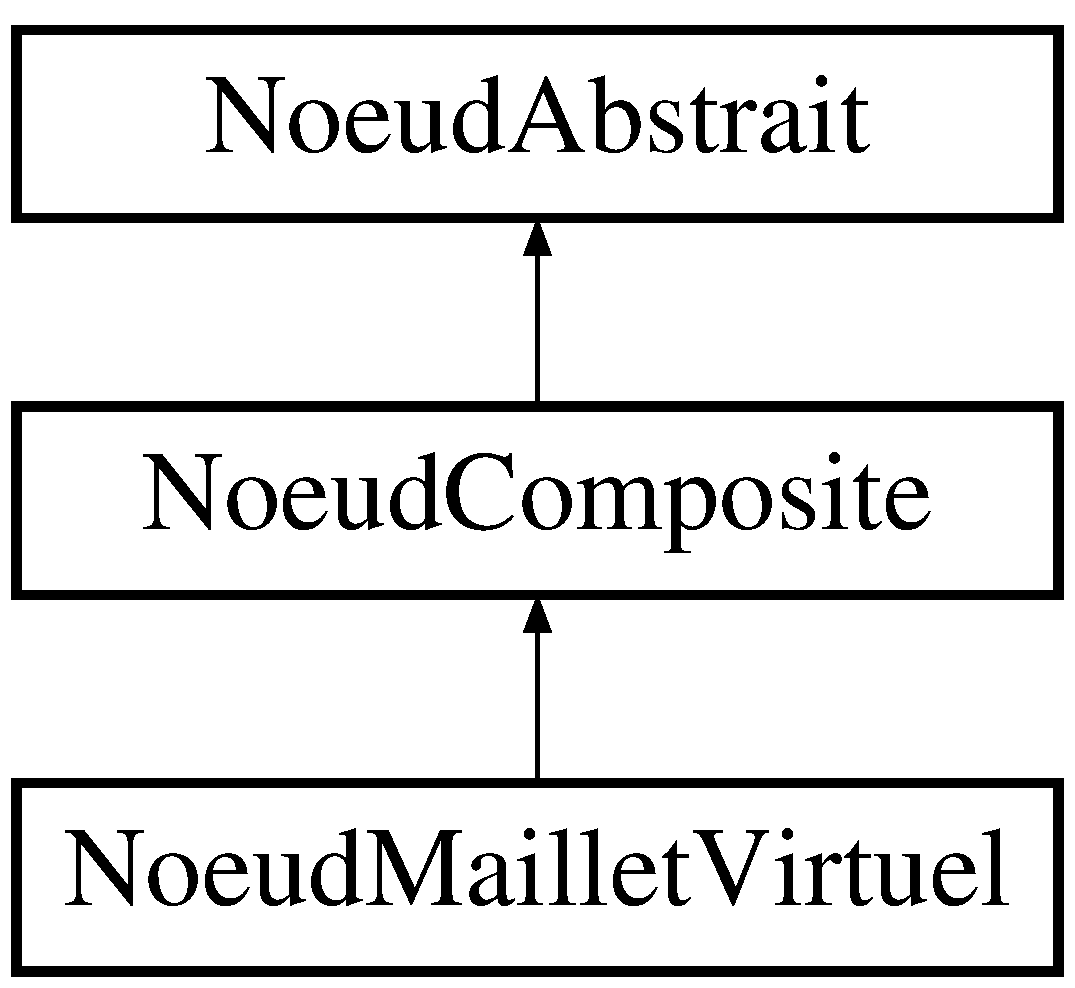
\includegraphics[height=3.000000cm]{class_noeud_maillet_virtuel}
\end{center}
\end{figure}
\subsection*{Public Member Functions}
\begin{DoxyCompactItemize}
\item 
\hyperlink{group__inf2990_ga59b290e7c237093d2f912f5280d2f5af}{Noeud\+Maillet\+Virtuel} (const std\+::string \&type\+Noeud)
\begin{DoxyCompactList}\small\item\em Constructeur � partir du type du noeud. \end{DoxyCompactList}\item 
virtual \hyperlink{group__inf2990_ga03d899ca4f3d8ff34904c14576c124e2}{$\sim$\+Noeud\+Maillet\+Virtuel} ()
\begin{DoxyCompactList}\small\item\em Destructeur. \end{DoxyCompactList}\item 
\hyperlink{group__inf2990_ga07c7521b475fa3617bb39fc803fb4b1e}{Noeud\+Maillet\+Virtuel} (\hyperlink{class_noeud_maillet_virtuel}{Noeud\+Maillet\+Virtuel} \&destination)
\begin{DoxyCompactList}\small\item\em Methode utiliser pour la copie des attributs. \end{DoxyCompactList}\item 
virtual void \hyperlink{group__inf2990_ga39980c2a4c8326e2d5c6b27029122c6f}{afficher\+Concret} (const glm\+::mat4 \&vue\+Projection, const bool \&attribuer\+Couleur) const
\begin{DoxyCompactList}\small\item\em Affiche le cube. \end{DoxyCompactList}\item 
void \hyperlink{group__inf2990_gae8437fedcad91a0ed2de8a52ab3f75e0}{moveY} (double temps)
\item 
void \hyperlink{group__inf2990_ga415fd16f7eb229e23f7323b690f17c1b}{moveX} (double temps)
\item 
virtual void \hyperlink{group__inf2990_ga01ed83c56c34e158f99bc0e5510eb3a7}{animer} (float temps)
\begin{DoxyCompactList}\small\item\em Effectue l\textquotesingle{}animation du cube. \end{DoxyCompactList}\item 
bool \hyperlink{group__inf2990_ga0e377ea81a936ab1071ef05bb2616da0}{verifier\+Selection} (G\+Lubyte couleur\+Objet\mbox{[}$\,$\mbox{]})
\item 
void \hyperlink{group__inf2990_gab8d0fbb388595cc40c630ae5f3fcd18e}{accepter\+Visiteur} (\hyperlink{class_visiteur_abstrait}{Visiteur\+Abstrait} $\ast$visiteur)
\item 
void {\bfseries modifier\+Rayon\+Maillet} (double rayon\+Maillet)
\item 
double {\bfseries obtenir\+Rayon\+MailletV} ()
\item 
void \hyperlink{group__inf2990_ga67ed45ef7581873709d171c69729c5d5}{assigner\+Probabilite\+De\+Jeu} (double proba)
\item 
void \hyperlink{group__inf2990_gaf2e3b81ef042d258771f7808e49a8585}{assigner\+Rondelle} (\hyperlink{class_noeud_rondelle}{Noeud\+Rondelle} $\ast$rondelle)
\begin{DoxyCompactList}\small\item\em assigner Rondelle \end{DoxyCompactList}\item 
void \hyperlink{group__inf2990_gaee9cb04c75df57917c44edffdeec703e}{assigner\+Vitesse} (double vitesse)
\begin{DoxyCompactList}\small\item\em assigner Vitesse \end{DoxyCompactList}\item 
double {\bfseries obtenir\+Vitesse} ()
\item 
void \hyperlink{group__inf2990_gad03b43314351abf5a165d2d5cab18684}{assigner\+Largeur\+Buts} (int largeur\+Buts)
\begin{DoxyCompactList}\small\item\em assigner la demi largeur des buts \end{DoxyCompactList}\item 
void \hyperlink{group__inf2990_ga9ab7cf88d41523c617e19adc9f91d946}{assigner\+Objet\+Rendu} (modele\+::\+Modele3D const $\ast$modele, opengl\+::\+V\+BO const $\ast$liste) override
\item 
virtual void \hyperlink{group__inf2990_ga4f44cafa4f84145ef6fa7d547cea7b1b}{redefinir\+Sommets} ()
\item 
bool \hyperlink{group__inf2990_gad20bce4c9afb2a635fe4d0957b6681e7}{est\+Dans\+La\+Table} ()
\end{DoxyCompactItemize}
\subsection*{Additional Inherited Members}


The documentation for this class was generated from the following files\+:\begin{DoxyCompactItemize}
\item 
Sources/\+D\+L\+L/\+Arbre/\+Noeuds/\hyperlink{_noeud_maillet_virtuel_8h}{Noeud\+Maillet\+Virtuel.\+h}\item 
Sources/\+D\+L\+L/\+Arbre/\+Noeuds/\hyperlink{_noeud_maillet_virtuel_8cpp}{Noeud\+Maillet\+Virtuel.\+cpp}\end{DoxyCompactItemize}

\hypertarget{class_noeud_muret}{}\section{Noeud\+Muret Class Reference}
\label{class_noeud_muret}\index{Noeud\+Muret@{Noeud\+Muret}}
Inheritance diagram for Noeud\+Muret\+:\begin{figure}[H]
\begin{center}
\leavevmode
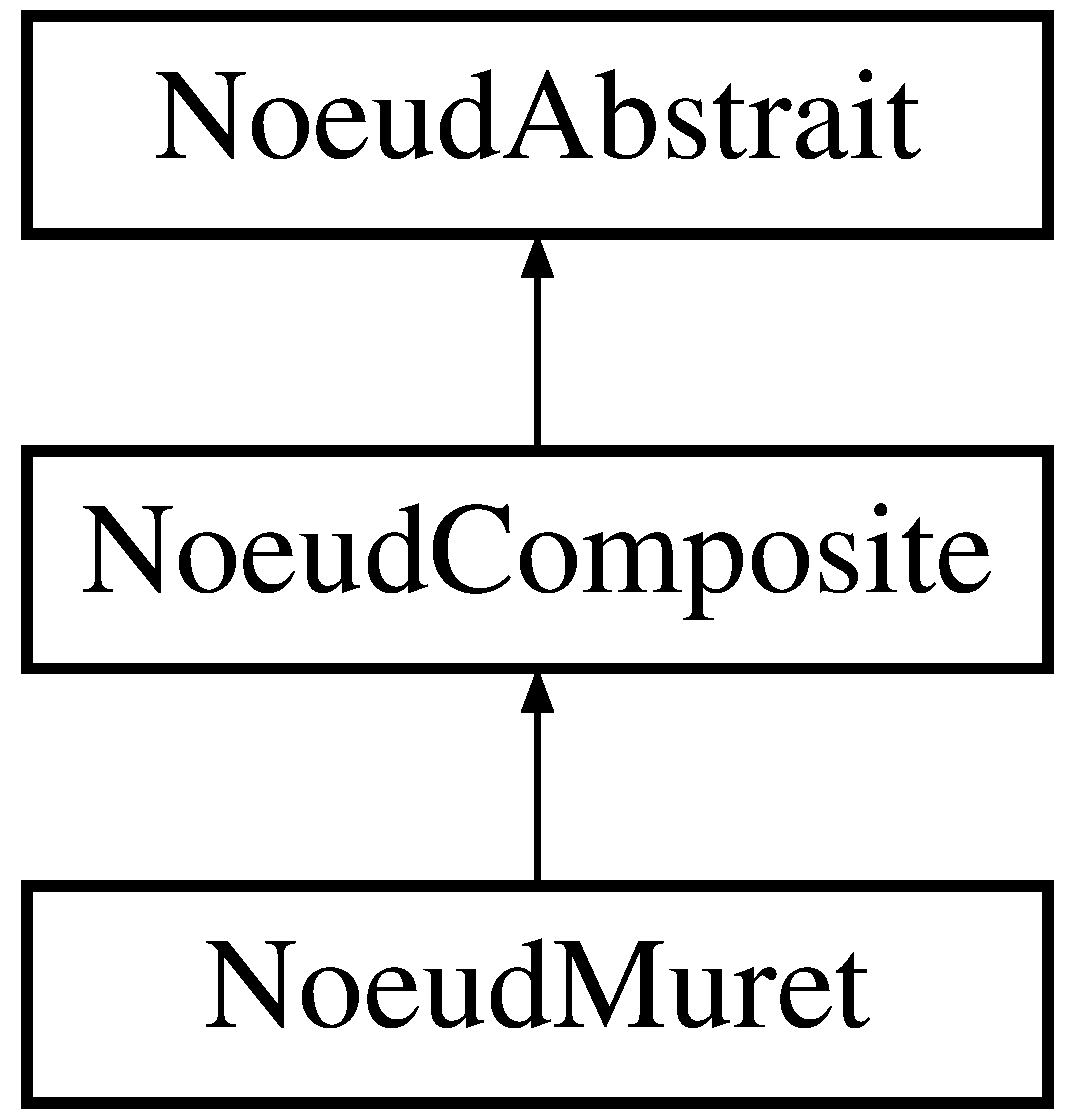
\includegraphics[height=3.000000cm]{class_noeud_muret}
\end{center}
\end{figure}
\subsection*{Classes}
\begin{DoxyCompactItemize}
\item 
struct \hyperlink{struct_noeud_muret_1_1point__muret}{point\+\_\+muret}
\begin{DoxyCompactList}\small\item\em Points du mur. \end{DoxyCompactList}\end{DoxyCompactItemize}
\subsection*{Public Member Functions}
\begin{DoxyCompactItemize}
\item 
\hyperlink{group__inf2990_gaed79ffb9953bf45a71b81e283bd5fbce}{Noeud\+Muret} (const std\+::string \&type\+Noeud)
\begin{DoxyCompactList}\small\item\em Constructeur � partir du type du noeud. \end{DoxyCompactList}\item 
\hyperlink{group__inf2990_ga98b208e791b2e3c257ab2ba403287fea}{$\sim$\+Noeud\+Muret} ()
\begin{DoxyCompactList}\small\item\em Destructeur. \end{DoxyCompactList}\item 
void {\bfseries copier\+Attributs} (\hyperlink{class_noeud_muret}{Noeud\+Muret} \&destination)
\item 
virtual void \hyperlink{group__inf2990_ga202d1ffab84dfcbcbcd6b4aae6ad848f}{afficher\+Concret} (const glm\+::mat4 \&vue\+Projection, const bool \&attribuer\+Couleur) const
\begin{DoxyCompactList}\small\item\em Affiche le cube. \end{DoxyCompactList}\item 
virtual void \hyperlink{group__inf2990_ga5acf4176b07c849da044bcd967cf4f34}{animer} (float temps)
\begin{DoxyCompactList}\small\item\em Effectue l\textquotesingle{}animation du cube. \end{DoxyCompactList}\item 
bool {\bfseries verifier\+Selection} (G\+Lubyte couleur\+Objet\mbox{[}$\,$\mbox{]})
\item 
void \hyperlink{group__inf2990_ga15f9180746601a312860373419f41349}{accepter\+Visiteur} (\hyperlink{class_visiteur_abstrait}{Visiteur\+Abstrait} $\ast$visiteur)
\item 
void {\bfseries modifier\+Longueur\+Muret} (double longueur\+Muret)
\item 
void \hyperlink{group__inf2990_ga0d2e1c77bf313d3459a8becddfce48f2}{assigner\+Objet\+Rendu} (modele\+::\+Modele3D const $\ast$modele, opengl\+::\+V\+BO const $\ast$liste) override
\begin{DoxyCompactList}\small\item\em Assigne la position initiale du noeud. \end{DoxyCompactList}\item 
virtual void {\bfseries redefinir\+Sommets} ()
\item 
virtual bool \hyperlink{group__inf2990_gac96032cddfa07f4bbbcc46b4ad818566}{est\+Dans\+La\+Table} ()
\begin{DoxyCompactList}\small\item\em permet de verifier si un objet est toujours a l\textquotesingle{}interieur de la table. \end{DoxyCompactList}\item 
double {\bfseries obtenir\+Longueur\+Muret} ()
\item 
\hyperlink{struct_noeud_muret_1_1point__muret}{point\+\_\+muret} \hyperlink{group__inf2990_gae5924b26388fe8937399bd9796e32caf}{obtenir\+Points} () const
\end{DoxyCompactItemize}
\subsection*{Additional Inherited Members}


The documentation for this class was generated from the following files\+:\begin{DoxyCompactItemize}
\item 
Sources/\+D\+L\+L/\+Arbre/\+Noeuds/\hyperlink{_noeud_muret_8h}{Noeud\+Muret.\+h}\item 
Sources/\+D\+L\+L/\+Arbre/\+Noeuds/Noeud\+Muret.\+cpp\end{DoxyCompactItemize}

\hypertarget{class_noeud_portail}{}\section{Noeud\+Portail Class Reference}
\label{class_noeud_portail}\index{Noeud\+Portail@{Noeud\+Portail}}
Inheritance diagram for Noeud\+Portail\+:\begin{figure}[H]
\begin{center}
\leavevmode
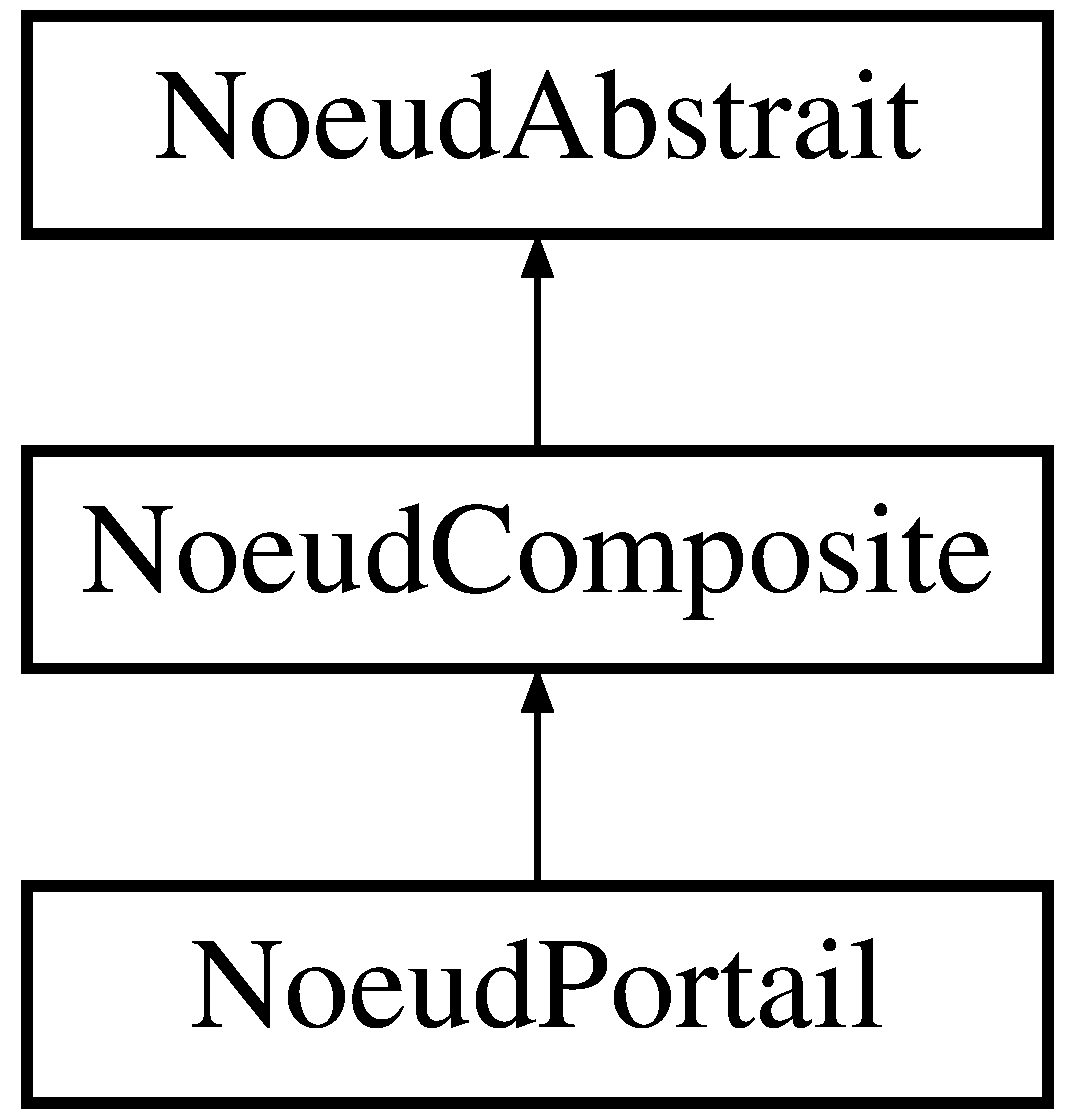
\includegraphics[height=3.000000cm]{class_noeud_portail}
\end{center}
\end{figure}
\subsection*{Public Member Functions}
\begin{DoxyCompactItemize}
\item 
\hyperlink{group__inf2990_ga1ae16fc50c4afaf88b5d4068868acac1}{Noeud\+Portail} (const std\+::string \&type\+Noeud)
\begin{DoxyCompactList}\small\item\em Constructeur � partir du type du noeud. \end{DoxyCompactList}\item 
\hyperlink{group__inf2990_ga539e125201edd719886ae550eab35a28}{$\sim$\+Noeud\+Portail} ()
\begin{DoxyCompactList}\small\item\em Destructeur. \end{DoxyCompactList}\item 
void {\bfseries copier\+Attributs} (\hyperlink{class_noeud_portail}{Noeud\+Portail} \&destination)
\item 
virtual void \hyperlink{group__inf2990_ga996fc8426391dd48ef70cfbd5132fb86}{afficher\+Concret} (const glm\+::mat4 \&vue\+Projection, const bool \&attribuer\+Couleur) const
\begin{DoxyCompactList}\small\item\em Affiche le cube. \end{DoxyCompactList}\item 
virtual void \hyperlink{group__inf2990_ga471730293ee98a18df3b4273db841f26}{accepter\+Visiteur} (\hyperlink{class_visiteur_abstrait}{Visiteur\+Abstrait} $\ast$visiteur)
\item 
virtual void \hyperlink{group__inf2990_ga74228e2bf740f880cf4d73f3f6ca4dc9}{animer} (float temps)
\begin{DoxyCompactList}\small\item\em Effectue l\textquotesingle{}animation du cube. \end{DoxyCompactList}\item 
\hypertarget{class_noeud_portail_a51f50d27f1324691e3e638a5580b5319}{}\label{class_noeud_portail_a51f50d27f1324691e3e638a5580b5319} 
bool {\bfseries obtenir\+Attraction} ()
\item 
virtual bool \hyperlink{group__inf2990_ga18f1b34d1f58ce8e140ddb3c9c4a5c1f}{verifier\+Selection} (G\+Lubyte couleur\+Objet\mbox{[}$\,$\mbox{]})
\item 
double \hyperlink{group__inf2990_gae66f8d1fe91f71fd8692a93d34be4aca}{obtenir\+Rayon\+Attraction} ()
\item 
\hyperlink{class_noeud_portail}{Noeud\+Portail} $\ast$ {\bfseries get\+Frere} ()
\item 
void {\bfseries set\+Frere} (\hyperlink{class_noeud_portail}{Noeud\+Portail} $\ast$noeud)
\item 
void {\bfseries modifier\+Rayon\+Portail} (double rayon\+Portail)
\item 
double {\bfseries obtenir\+Rayon\+Portail} ()
\end{DoxyCompactItemize}
\subsection*{Additional Inherited Members}


The documentation for this class was generated from the following files\+:\begin{DoxyCompactItemize}
\item 
Sources/\+D\+L\+L/\+Arbre/\+Noeuds/\hyperlink{_noeud_portail_8h}{Noeud\+Portail.\+h}\item 
Sources/\+D\+L\+L/\+Arbre/\+Noeuds/Noeud\+Portail.\+cpp\end{DoxyCompactItemize}

\hypertarget{class_noeud_rondelle}{}\section{Noeud\+Rondelle Class Reference}
\label{class_noeud_rondelle}\index{Noeud\+Rondelle@{Noeud\+Rondelle}}


Classe qui repr�sente un exemple de noeud de l\textquotesingle{}arbre de rendu.  




{\ttfamily \#include $<$Noeud\+Rondelle.\+h$>$}

Inheritance diagram for Noeud\+Rondelle\+:\begin{figure}[H]
\begin{center}
\leavevmode
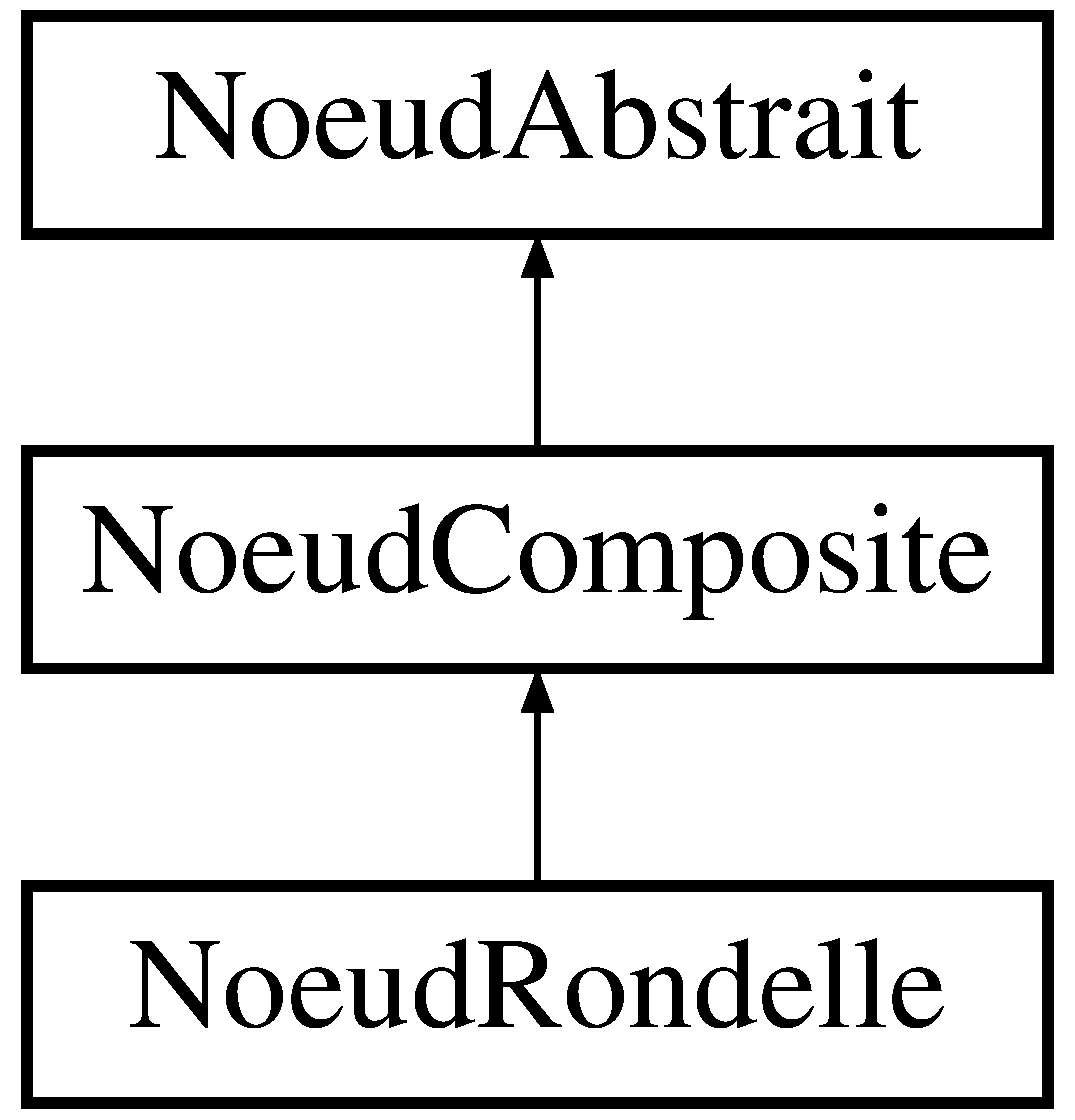
\includegraphics[height=3.000000cm]{class_noeud_rondelle}
\end{center}
\end{figure}
\subsection*{Public Member Functions}
\begin{DoxyCompactItemize}
\item 
\hyperlink{group__inf2990_ga34a329c95e92769fb7ee559f9d8190ee}{Noeud\+Rondelle} (const std\+::string \&type\+Noeud)
\begin{DoxyCompactList}\small\item\em Constructeur � partir du type du noeud. \end{DoxyCompactList}\item 
{\bfseries Noeud\+Rondelle} (const \hyperlink{class_noeud_rondelle}{Noeud\+Rondelle} \&)
\item 
\hyperlink{group__inf2990_ga72fbc525724f54469d00c55052403581}{$\sim$\+Noeud\+Rondelle} ()
\begin{DoxyCompactList}\small\item\em Destructeur. \end{DoxyCompactList}\item 
void {\bfseries copier\+Attributs} (\hyperlink{class_noeud_rondelle}{Noeud\+Rondelle} \&destination)
\item 
virtual void \hyperlink{group__inf2990_gae36211d198101ecb9ad8f252a3483a8b}{afficher\+Concret} (const glm\+::mat4 \&vue\+Projection, const bool \&attribuer\+Couleur) const
\begin{DoxyCompactList}\small\item\em Affiche le cube. \end{DoxyCompactList}\item 
virtual void \hyperlink{group__inf2990_ga016689cb1c1968037902ae0013397bff}{animer} (float temps)
\begin{DoxyCompactList}\small\item\em Effectue l\textquotesingle{}animation du cube. \end{DoxyCompactList}\item 
void \hyperlink{group__inf2990_ga7a7dea6fa17b186ff6e619b2e8b29bd8}{modifier\+Rayon\+Rondelle} (double rayon\+Rondelle)
\item 
double \hyperlink{group__inf2990_ga514eb45118a873e6516557a25f31eb62}{obtenir\+Rayon\+Rondelle} ()
\item 
virtual void \hyperlink{group__inf2990_gac9e330d1fe7f2413474785b4f2280db5}{accepter\+Visiteur} (\hyperlink{class_visiteur_abstrait}{Visiteur\+Abstrait} $\ast$visiteur)
\end{DoxyCompactItemize}
\subsection*{Additional Inherited Members}


\subsection{Detailed Description}
Classe qui repr�sente un exemple de noeud de l\textquotesingle{}arbre de rendu. 

\begin{DoxyAuthor}{Author}
Equipe06 
\end{DoxyAuthor}
\begin{DoxyDate}{Date}
2016-\/09-\/07 
\end{DoxyDate}


The documentation for this class was generated from the following files\+:\begin{DoxyCompactItemize}
\item 
Sources/\+D\+L\+L/\+Arbre/\+Noeuds/\hyperlink{_noeud_rondelle_8h}{Noeud\+Rondelle.\+h}\item 
Sources/\+D\+L\+L/\+Arbre/\+Noeuds/\hyperlink{_noeud_maillet_8cpp}{Noeud\+Maillet.\+cpp}\item 
Sources/\+D\+L\+L/\+Arbre/\+Noeuds/Noeud\+Muret.\+cpp\item 
Sources/\+D\+L\+L/\+Arbre/\+Noeuds/Noeud\+Portail.\+cpp\item 
Sources/\+D\+L\+L/\+Arbre/\+Noeuds/Noeud\+Rondelle.\+cpp\end{DoxyCompactItemize}

\hypertarget{class_noeud_table}{}\section{Noeud\+Table Class Reference}
\label{class_noeud_table}\index{Noeud\+Table@{Noeud\+Table}}


Classe qui représente un exemple de noeud de l\textquotesingle{}arbre de rendu.  




{\ttfamily \#include $<$Noeud\+Table.\+h$>$}

Inheritance diagram for Noeud\+Table\+:\begin{figure}[H]
\begin{center}
\leavevmode
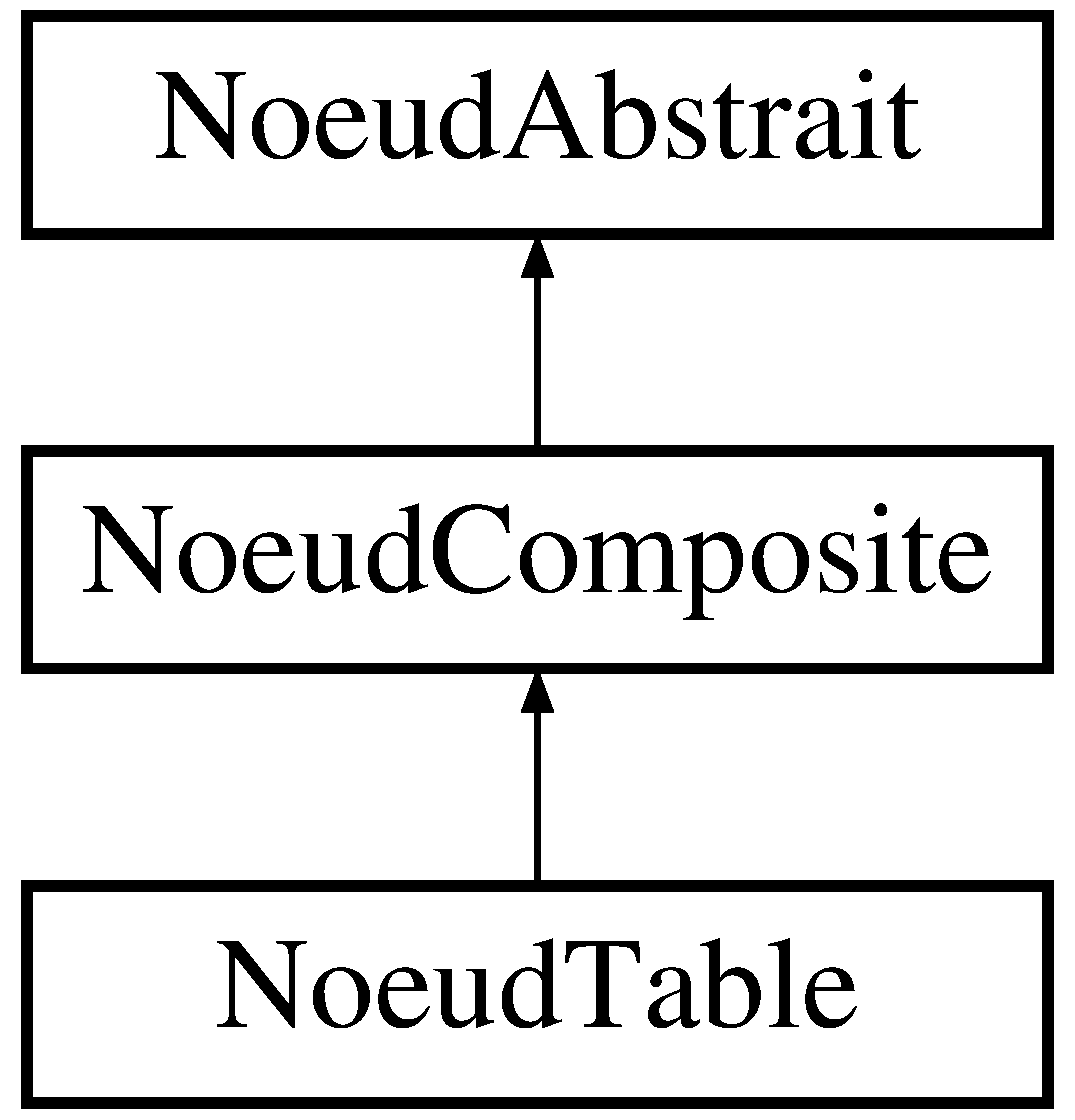
\includegraphics[height=3.000000cm]{class_noeud_table}
\end{center}
\end{figure}
\subsection*{Public Member Functions}
\begin{DoxyCompactItemize}
\item 
\hyperlink{group__inf2990_ga40983870720b331d17daeeb306e12ef5}{Noeud\+Table} (const std\+::string \&type\+Noeud)
\begin{DoxyCompactList}\small\item\em Constructeur à partir du type du noeud. \end{DoxyCompactList}\item 
\hyperlink{group__inf2990_ga6171c2df59de6f454f0d8c7915403ce7}{$\sim$\+Noeud\+Table} ()
\begin{DoxyCompactList}\small\item\em Destructeur. \end{DoxyCompactList}\item 
virtual void \hyperlink{group__inf2990_ga7e6bc962988899cf4ff7f2b1f9b51be9}{afficher\+Concret} (const glm\+::mat4 \&vue\+Projection, const bool \&attribuer\+Couleur) const
\begin{DoxyCompactList}\small\item\em Affiche le cube. \end{DoxyCompactList}\item 
virtual void \hyperlink{group__inf2990_gadf419e5147546815052d75529c4c45ab}{animer} (float temps)
\begin{DoxyCompactList}\small\item\em Effectue l\textquotesingle{}animation du cube. \end{DoxyCompactList}\item 
virtual void \hyperlink{group__inf2990_ga52e75d8d0ea0ac39c28b056245926f91}{redessiner} ()
\item 
void {\bfseries dessiner\+Carre} (glm\+::vec3 t) const
\item 
void {\bfseries dessiner\+Point\+De\+Controle} () const
\item 
virtual double \hyperlink{group__inf2990_ga0e66165b0be4a7994027c35201177903}{obtenir\+Friction} () const
\item 
void \hyperlink{group__inf2990_ga7e936cac741c4716548cb69ffde1777d}{modifier\+Friction} (double friction)
\item 
double \hyperlink{group__inf2990_ga6dd00515181d18b18cbc27292277b006}{obtenir\+Coef\+Rebondissement} ()
\item 
void \hyperlink{group__inf2990_ga3b11cdcbe4a4cf30095cd54083cd4019}{modifier\+Coef\+Rebondissement} (double coef\+Rebondissement)
\item 
double \hyperlink{group__inf2990_ga28011811ced7c04906780070a7762ec3}{obtenir\+Acceleration} ()
\item 
void \hyperlink{group__inf2990_ga1ac0745a780e04a265ee01bec42210e1}{modifier\+Acceleration} (double acceleration)
\item 
virtual void \hyperlink{group__inf2990_ga37c3779e4662401c1ed6fb64de2c43bf}{redefinir\+Sommets} ()
\item 
virtual bool \hyperlink{group__inf2990_ga4e59d47514e12d1bdcf3047ecc4230c9}{curseur\+Est\+Dans\+Table} (glm\+::dvec3 pos)
\item 
virtual bool {\bfseries curseur\+Est\+Dans\+Zone} (glm\+::dvec3 pos)
\item 
void {\bfseries chercher\+Collisions} ()
\item 
void {\bfseries assigner\+Rondelle} (\hyperlink{class_noeud_rondelle}{Noeud\+Rondelle} $\ast$rond)
\item 
void \hyperlink{group__inf2990_ga74c94e6298b50f2ce1b893da20d9662b}{definir\+Zone} ()
\item 
\hyperlink{class_noeud_rondelle}{Noeud\+Rondelle} $\ast$ {\bfseries obtenir\+Rondelle} ()
\item 
int {\bfseries get\+Gauche} ()
\item 
int {\bfseries get\+Droite} ()
\item 
void {\bfseries incrementer\+Gauche} ()
\item 
void {\bfseries incrementer\+Droite} ()
\item 
void {\bfseries reinitialiser\+But} ()
\end{DoxyCompactItemize}
\subsection*{Additional Inherited Members}


\subsection{Detailed Description}
Classe qui représente un exemple de noeud de l\textquotesingle{}arbre de rendu. 

\begin{DoxyAuthor}{Author}
Equipe06 
\end{DoxyAuthor}
\begin{DoxyDate}{Date}
2016-\/09-\/07 
\end{DoxyDate}


The documentation for this class was generated from the following files\+:\begin{DoxyCompactItemize}
\item 
Sources/\+D\+L\+L/\+Arbre/\+Noeuds/\hyperlink{_noeud_table_8h}{Noeud\+Table.\+h}\item 
Sources/\+D\+L\+L/\+Arbre/\+Noeuds/\hyperlink{_noeud_table_8cpp}{Noeud\+Table.\+cpp}\end{DoxyCompactItemize}

\hypertarget{class_partie}{}\section{Partie Class Reference}
\label{class_partie}\index{Partie@{Partie}}


Classe qui regroupe les parametres de de la partie.  




{\ttfamily \#include $<$Partie.\+h$>$}

\subsection*{Public Member Functions}
\begin{DoxyCompactItemize}
\item 
\hyperlink{group__inf2990_gae0fd466396b1f1da7f24106ea1336b7c}{Partie} (int nb\+But, bool joueur\+Virtuel)
\begin{DoxyCompactList}\small\item\em Constructueur pour une partie standard. \end{DoxyCompactList}\item 
{\bfseries Partie} (int nb\+But, bool joueur\+G\+Virtuel, std\+::string nomjoueurG, bool joueur\+D\+Virtuel, std\+::string nomjoueurD)
\item 
\hyperlink{group__inf2990_ga60f6de457bc2b70555f26964174303a7}{Partie} (int nb\+But, \hyperlink{class_noeud_joueur}{Noeud\+Joueur} $\ast$, \hyperlink{class_noeud_joueur}{Noeud\+Joueur} $\ast$)
\begin{DoxyCompactList}\small\item\em Constructueur pour une partie dans un tournoi. \end{DoxyCompactList}\item 
\hyperlink{group__inf2990_gae4afeb7336bb84427272cfb7018b5e3d}{$\sim$\+Partie} ()
\begin{DoxyCompactList}\small\item\em Destructeur. \end{DoxyCompactList}\item 
int {\bfseries obtenir\+But\+Joueur1} () const
\item 
int {\bfseries obtenir\+But\+Joueur2} () const
\item 
void {\bfseries assigner\+Joueur1} (\hyperlink{class_noeud_joueur}{Noeud\+Joueur} $\ast$)
\item 
void {\bfseries assigner\+Joueur1} (std\+::string)
\item 
void {\bfseries assigner\+Joueur2} (std\+::string)
\item 
void {\bfseries assigner\+Joueur2} (\hyperlink{class_noeud_joueur}{Noeud\+Joueur} $\ast$)
\item 
void {\bfseries assignerbut\+J1} ()
\item 
void {\bfseries assignerbut\+J2} ()
\item 
void {\bfseries mise\+En\+Place\+Maillet} (bool est\+Virtuel)
\item 
std\+::string {\bfseries obtenir\+Vainqueur} ()
\item 
void {\bfseries reinitialiser} ()
\item 
void {\bfseries arreter} ()
\item 
\hypertarget{class_partie_ac0747c32bd176efc2993a23100a44a0a}{}\label{class_partie_ac0747c32bd176efc2993a23100a44a0a} 
void {\bfseries charger\+Zone} (string nom\+Zone)
\item 
\hypertarget{class_partie_aa4e3abdd7d14f8d8e3fc1af5f1cdbdf8}{}\label{class_partie_aa4e3abdd7d14f8d8e3fc1af5f1cdbdf8} 
bool {\bfseries get\+Etat\+Partie} ()
\item 
\hypertarget{class_partie_ab88eb7e47b3da834363f2534786211fb}{}\label{class_partie_ab88eb7e47b3da834363f2534786211fb} 
void {\bfseries set\+Etat\+Partie} (bool a)
\end{DoxyCompactItemize}
\subsection*{Public Attributes}
\begin{DoxyCompactItemize}
\item 
\hypertarget{class_partie_a7d70f99d8f87219f2ddeaebc9773a623}{}\label{class_partie_a7d70f99d8f87219f2ddeaebc9773a623} 
\hyperlink{class_facade_modele}{Facade\+Modele} $\ast$ {\bfseries facade}
\end{DoxyCompactItemize}


\subsection{Detailed Description}
Classe qui regroupe les parametres de de la partie. 

\begin{DoxyAuthor}{Author}
equipe06 
\end{DoxyAuthor}
\begin{DoxyDate}{Date}
2016-\/10-\/20 
\end{DoxyDate}


The documentation for this class was generated from the following files\+:\begin{DoxyCompactItemize}
\item 
Sources/\+D\+L\+L/\+Application/Partie.\+h\item 
Sources/\+D\+L\+L/\+Application/Partie.\+cpp\end{DoxyCompactItemize}

\hypertarget{class_interface_graphique_1_1_partie_rapide}{}\section{Interface\+Graphique.\+Partie\+Rapide Class Reference}
\label{class_interface_graphique_1_1_partie_rapide}\index{Interface\+Graphique.\+Partie\+Rapide@{Interface\+Graphique.\+Partie\+Rapide}}
Inheritance diagram for Interface\+Graphique.\+Partie\+Rapide\+:\begin{figure}[H]
\begin{center}
\leavevmode
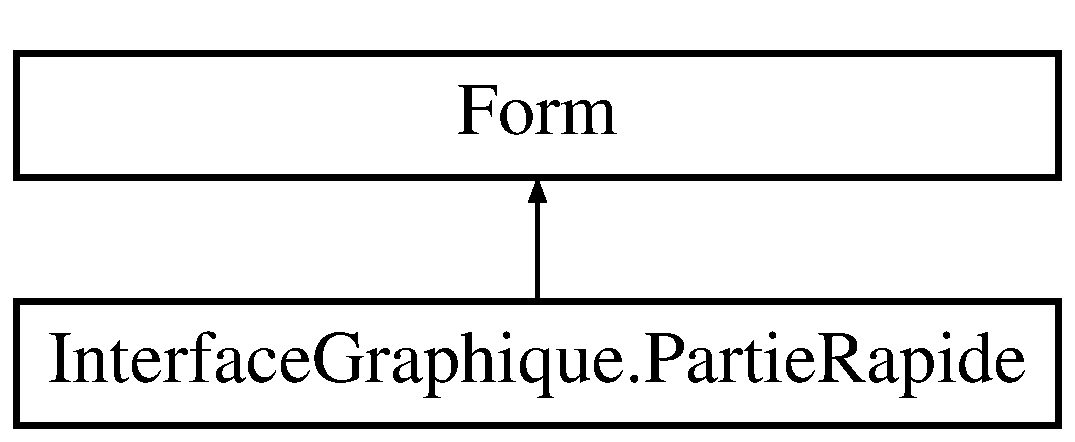
\includegraphics[height=2.000000cm]{class_interface_graphique_1_1_partie_rapide}
\end{center}
\end{figure}
\subsection*{Public Member Functions}
\begin{DoxyCompactItemize}
\item 
void \hyperlink{group__inf2990_gaf5ff96f0fca70376fe5e1a69565eb592}{Initialiser\+Animation} ()
\begin{DoxyCompactList}\small\item\em Initialiser les animations. \end{DoxyCompactList}\item 
void {\bfseries Mettre\+A\+Jour} (double temps\+Inter\+Affichage)
\end{DoxyCompactItemize}
\subsection*{Protected Member Functions}
\begin{DoxyCompactItemize}
\item 
override bool \hyperlink{group__inf2990_ga7dac506aec410200b7f6600ecf06b57b}{Process\+Cmd\+Key} (ref Message msg, Keys key\+Data)
\begin{DoxyCompactList}\small\item\em Pour afficher la barre de menu avec le bouton E\+SC. \end{DoxyCompactList}\item 
override void \hyperlink{class_interface_graphique_1_1_partie_rapide_a248957e40a9fe9d9ca2e3c90e117b192}{Dispose} (bool disposing)
\begin{DoxyCompactList}\small\item\em Clean up any resources being used. \end{DoxyCompactList}\end{DoxyCompactItemize}


\subsection{Member Function Documentation}
\hypertarget{class_interface_graphique_1_1_partie_rapide_a248957e40a9fe9d9ca2e3c90e117b192}{}\label{class_interface_graphique_1_1_partie_rapide_a248957e40a9fe9d9ca2e3c90e117b192} 
\index{Interface\+Graphique\+::\+Partie\+Rapide@{Interface\+Graphique\+::\+Partie\+Rapide}!Dispose@{Dispose}}
\index{Dispose@{Dispose}!Interface\+Graphique\+::\+Partie\+Rapide@{Interface\+Graphique\+::\+Partie\+Rapide}}
\subsubsection{\texorpdfstring{Dispose()}{Dispose()}}
{\footnotesize\ttfamily override void Interface\+Graphique.\+Partie\+Rapide.\+Dispose (\begin{DoxyParamCaption}\item[{bool}]{disposing }\end{DoxyParamCaption})\hspace{0.3cm}{\ttfamily [inline]}, {\ttfamily [protected]}}



Clean up any resources being used. 


\begin{DoxyParams}{Parameters}
{\em disposing} & true if managed resources should be disposed; otherwise, false.\\
\hline
\end{DoxyParams}


The documentation for this class was generated from the following files\+:\begin{DoxyCompactItemize}
\item 
C\+:/\+Users/\+Steven/\+Documents/\+Poly/\+I\+N\+F2990/inf2990-\/06/\+Cadriciel\+\_\+2016-\/3\+\_\+\+Etudiants/\+Cadriciel/\+Sources/\+Interface\+Graphique/\hyperlink{_partie_rapide_8cs}{Partie\+Rapide.\+cs}\item 
C\+:/\+Users/\+Steven/\+Documents/\+Poly/\+I\+N\+F2990/inf2990-\/06/\+Cadriciel\+\_\+2016-\/3\+\_\+\+Etudiants/\+Cadriciel/\+Sources/\+Interface\+Graphique/Partie\+Rapide.\+Designer.\+cs\end{DoxyCompactItemize}

\hypertarget{struct_noeud_muret_1_1point__muret}{}\section{Noeud\+Muret\+:\+:point\+\_\+muret Struct Reference}
\label{struct_noeud_muret_1_1point__muret}\index{Noeud\+Muret\+::point\+\_\+muret@{Noeud\+Muret\+::point\+\_\+muret}}


Points du mur.  




{\ttfamily \#include $<$Noeud\+Muret.\+h$>$}

\subsection*{Public Member Functions}
\begin{DoxyCompactItemize}
\item 
\hypertarget{struct_noeud_muret_1_1point__muret_ac69905e3fbbfe9a0453ab78cb20aa44b}{}\label{struct_noeud_muret_1_1point__muret_ac69905e3fbbfe9a0453ab78cb20aa44b} 
{\bfseries point\+\_\+muret} (const glm\+::dvec3 \&p1, const glm\+::dvec3 \&p2)
\end{DoxyCompactItemize}
\subsection*{Public Attributes}
\begin{DoxyCompactItemize}
\item 
\hypertarget{struct_noeud_muret_1_1point__muret_a294381a61a5e78afcdb60902dee1c3c5}{}\label{struct_noeud_muret_1_1point__muret_a294381a61a5e78afcdb60902dee1c3c5} 
glm\+::dvec3 {\bfseries debut}
\item 
\hypertarget{struct_noeud_muret_1_1point__muret_ad2a2e0f42dd5c60dec0489cfe82ecb98}{}\label{struct_noeud_muret_1_1point__muret_ad2a2e0f42dd5c60dec0489cfe82ecb98} 
glm\+::dvec3 {\bfseries fin}
\end{DoxyCompactItemize}


\subsection{Detailed Description}
Points du mur. 

The documentation for this struct was generated from the following file\+:\begin{DoxyCompactItemize}
\item 
C\+:/\+Users/\+Steven/\+Documents/\+Poly/\+I\+N\+F2990/inf2990-\/06/\+Cadriciel\+\_\+2016-\/3\+\_\+\+Etudiants/\+Cadriciel/\+Sources/\+D\+L\+L/\+Arbre/\+Noeuds/\hyperlink{_noeud_muret_8h}{Noeud\+Muret.\+h}\end{DoxyCompactItemize}

\hypertarget{structposition}{}\section{position Struct Reference}
\label{structposition}\index{position@{position}}
\subsection*{Public Attributes}
\begin{DoxyCompactItemize}
\item 
\hypertarget{structposition_a216a393164d184a43ac6951f03aa81de}{}\label{structposition_a216a393164d184a43ac6951f03aa81de} 
float {\bfseries X}
\item 
\hypertarget{structposition_a357b87e4e84ff9f209f164cacbf8beae}{}\label{structposition_a357b87e4e84ff9f209f164cacbf8beae} 
float {\bfseries Y}
\end{DoxyCompactItemize}


The documentation for this struct was generated from the following file\+:\begin{DoxyCompactItemize}
\item 
Sources/\+D\+L\+L/Visiteur\+Rotation.\+h\end{DoxyCompactItemize}

\hypertarget{struct_interface_graphique_1_1_profil}{}\section{Interface\+Graphique.\+Profil Struct Reference}
\label{struct_interface_graphique_1_1_profil}\index{Interface\+Graphique.\+Profil@{Interface\+Graphique.\+Profil}}
\subsection*{Public Member Functions}
\begin{DoxyCompactItemize}
\item 
{\bfseries Profil} (string c\+Nom, int c\+Vitesse, int c\+Passivite)
\end{DoxyCompactItemize}
\subsection*{Public Attributes}
\begin{DoxyCompactItemize}
\item 
string {\bfseries nom}
\item 
int {\bfseries vitesse}
\item 
int {\bfseries passivite}
\end{DoxyCompactItemize}


The documentation for this struct was generated from the following file\+:\begin{DoxyCompactItemize}
\item 
Sources/\+Interface\+Graphique/\hyperlink{_configuration_8cs}{Configuration.\+cs}\end{DoxyCompactItemize}

\hypertarget{class_profil_virtuel}{}\section{Profil\+Virtuel Class Reference}
\label{class_profil_virtuel}\index{Profil\+Virtuel@{Profil\+Virtuel}}
\subsection*{Public Member Functions}
\begin{DoxyCompactItemize}
\item 
\hyperlink{group__inf2990_ga0d0539c487d998663383f6fee4005e56}{Profil\+Virtuel} ()
\begin{DoxyCompactList}\small\item\em Constructeur par defaut. \end{DoxyCompactList}\item 
\hyperlink{group__inf2990_gab78b313efeeb5d5e15a37e6eff294858}{Profil\+Virtuel} (std\+::string nom, int vitesse, int passivite)
\begin{DoxyCompactList}\small\item\em Constructeur par parametres qui prend le nom, la vitesse et le degre de passivite. \end{DoxyCompactList}\item 
const char $\ast$ {\bfseries obtenir\+Nom} ()
\item 
int {\bfseries obtenir\+Vitesse} ()
\item 
int {\bfseries obtenir\+Passivite} ()
\item 
void {\bfseries modifier\+Nom} (char $\ast$nom)
\item 
void {\bfseries modifier\+Vitesse} (int vitesse)
\item 
void {\bfseries modifier\+Passivite} (int passivite)
\end{DoxyCompactItemize}


The documentation for this class was generated from the following files\+:\begin{DoxyCompactItemize}
\item 
C\+:/\+Users/\+Steven/\+Documents/\+Poly/\+I\+N\+F2990/inf2990-\/06/\+Cadriciel\+\_\+2016-\/3\+\_\+\+Etudiants/\+Cadriciel/\+Sources/\+D\+L\+L/Profil\+Virtuel.\+h\item 
C\+:/\+Users/\+Steven/\+Documents/\+Poly/\+I\+N\+F2990/inf2990-\/06/\+Cadriciel\+\_\+2016-\/3\+\_\+\+Etudiants/\+Cadriciel/\+Sources/\+D\+L\+L/Profil\+Virtuel.\+cpp\end{DoxyCompactItemize}

\hypertarget{class_interface_graphique_1_1_propri_xC3_xA9t_xC3_xA9s}{}\section{Interface\+Graphique.\+Propriétés Class Reference}
\label{class_interface_graphique_1_1_propri_xC3_xA9t_xC3_xA9s}\index{Interface\+Graphique.\+Propriétés@{Interface\+Graphique.\+Propriétés}}
Inheritance diagram for Interface\+Graphique.\+Propriétés\+:\begin{figure}[H]
\begin{center}
\leavevmode
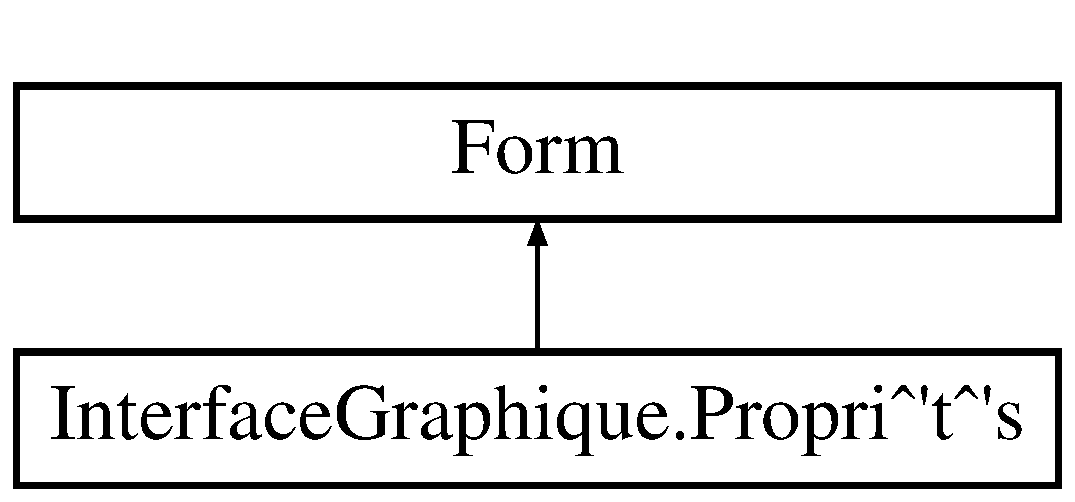
\includegraphics[height=2.000000cm]{class_interface_graphique_1_1_propri_xC3_xA9t_xC3_xA9s}
\end{center}
\end{figure}
\subsection*{Protected Member Functions}
\begin{DoxyCompactItemize}
\item 
override void \hyperlink{class_interface_graphique_1_1_propri_xC3_xA9t_xC3_xA9s_a3d9a2d4aa0c5ff07def08a4867803ada}{Dispose} (bool disposing)
\begin{DoxyCompactList}\small\item\em Clean up any resources being used. \end{DoxyCompactList}\end{DoxyCompactItemize}


\subsection{Member Function Documentation}
\hypertarget{class_interface_graphique_1_1_propri_xC3_xA9t_xC3_xA9s_a3d9a2d4aa0c5ff07def08a4867803ada}{}\label{class_interface_graphique_1_1_propri_xC3_xA9t_xC3_xA9s_a3d9a2d4aa0c5ff07def08a4867803ada} 
\index{Interface\+Graphique\+::\+Propriétés@{Interface\+Graphique\+::\+Propriétés}!Dispose@{Dispose}}
\index{Dispose@{Dispose}!Interface\+Graphique\+::\+Propriétés@{Interface\+Graphique\+::\+Propriétés}}
\subsubsection{\texorpdfstring{Dispose()}{Dispose()}}
{\footnotesize\ttfamily override void Interface\+Graphique.\+Propriétés.\+Dispose (\begin{DoxyParamCaption}\item[{bool}]{disposing }\end{DoxyParamCaption})\hspace{0.3cm}{\ttfamily [inline]}, {\ttfamily [protected]}}



Clean up any resources being used. 


\begin{DoxyParams}{Parameters}
{\em disposing} & true if managed resources should be disposed; otherwise, false.\\
\hline
\end{DoxyParams}


The documentation for this class was generated from the following files\+:\begin{DoxyCompactItemize}
\item 
C\+:/\+Users/\+Steven/\+Documents/\+Poly/\+I\+N\+F2990/inf2990-\/06/\+Cadriciel\+\_\+2016-\/3\+\_\+\+Etudiants/\+Cadriciel/\+Sources/\+Interface\+Graphique/Propriétés.\+cs\item 
C\+:/\+Users/\+Steven/\+Documents/\+Poly/\+I\+N\+F2990/inf2990-\/06/\+Cadriciel\+\_\+2016-\/3\+\_\+\+Etudiants/\+Cadriciel/\+Sources/\+Interface\+Graphique/Propriétés.\+Designer.\+cs\end{DoxyCompactItemize}

\hypertarget{class_texture}{}\section{Texture Class Reference}
\label{class_texture}\index{Texture@{Texture}}
\subsection*{Public Member Functions}
\begin{DoxyCompactItemize}
\item 
void \hyperlink{group__inf2990_gac2b173a88bb31605ada337fa22d0bfe1}{charger\+Texture} ()
\item 
unsigned int \hyperlink{group__inf2990_gaecb17eb4139fc2afbb7b739a0c5a55e8}{obtenir\+Texture\+Muret} () const
\begin{DoxyCompactList}\small\item\em retourne la texture des murets \end{DoxyCompactList}\item 
unsigned int \hyperlink{group__inf2990_ga8f333a9c5eb6d95a0acad97c94987d7d}{obtenir\+Texture\+Glace} () const
\begin{DoxyCompactList}\small\item\em retourne la texture de la glace \end{DoxyCompactList}\item 
unsigned int {\bfseries obtenir\+Ligne\+Milieu} () const
\item 
unsigned int {\bfseries obtenir\+Texturetexture\+But} () const
\item 
unsigned int \hyperlink{group__inf2990_ga811bcd121f45ed6f1817b9c19e90eb56}{obtenir\+Texture\+Bordure} (int index) const
\begin{DoxyCompactList}\small\item\em retourne la texture de la bordure \end{DoxyCompactList}\end{DoxyCompactItemize}
\subsection*{Static Public Member Functions}
\begin{DoxyCompactItemize}
\item 
static \hyperlink{class_texture}{Texture} $\ast$ \hyperlink{group__inf2990_ga9e983f4c36a7135b480a2f72e2daa988}{obtenir\+Instance} ()
\begin{DoxyCompactList}\small\item\em Obtient l\textquotesingle{}instance unique de la classe. \end{DoxyCompactList}\item 
static void \hyperlink{group__inf2990_gaf9a59e72caaedb7e73e422de71fba261}{liberer\+Instance} ()
\begin{DoxyCompactList}\small\item\em Lib�re l\textquotesingle{}instance unique de la classe. \end{DoxyCompactList}\end{DoxyCompactItemize}


The documentation for this class was generated from the following files\+:\begin{DoxyCompactItemize}
\item 
C\+:/\+Users/\+Steven/\+Documents/\+Poly/\+I\+N\+F2990/inf2990-\/06/\+Cadriciel\+\_\+2016-\/3\+\_\+\+Etudiants/\+Cadriciel/\+Sources/\+D\+L\+L/\+Arbre/Texture.\+h\item 
C\+:/\+Users/\+Steven/\+Documents/\+Poly/\+I\+N\+F2990/inf2990-\/06/\+Cadriciel\+\_\+2016-\/3\+\_\+\+Etudiants/\+Cadriciel/\+Sources/\+D\+L\+L/\+Arbre/\hyperlink{_texture_8cpp}{Texture.\+cpp}\end{DoxyCompactItemize}

\hypertarget{class_textures}{}\section{Textures Class Reference}
\label{class_textures}\index{Textures@{Textures}}


cette classe nous permet de charger toutes les textures en une fois  




{\ttfamily \#include $<$Texture.\+h$>$}



\subsection{Detailed Description}
cette classe nous permet de charger toutes les textures en une fois 

\begin{DoxyAuthor}{Author}
equipe06 
\end{DoxyAuthor}
\begin{DoxyDate}{Date}
2016-\/09-\/08 
\end{DoxyDate}


The documentation for this class was generated from the following file\+:\begin{DoxyCompactItemize}
\item 
C\+:/\+Users/\+Steven/\+Documents/\+Poly/\+I\+N\+F2990/inf2990-\/06/\+Cadriciel\+\_\+2016-\/3\+\_\+\+Etudiants/\+Cadriciel/\+Sources/\+D\+L\+L/\+Arbre/Texture.\+h\end{DoxyCompactItemize}

\hypertarget{class_tournoi}{}\section{Tournoi Class Reference}
\label{class_tournoi}\index{Tournoi@{Tournoi}}


Classe qui regroupe les parametres du tournoi.  




{\ttfamily \#include $<$Tournoi.\+h$>$}

\subsection*{Public Member Functions}
\begin{DoxyCompactItemize}
\item 
\hypertarget{class_tournoi_aef3539df119116b9bd69feff6c1e0c80}{}\label{class_tournoi_aef3539df119116b9bd69feff6c1e0c80} 
void {\bfseries assigner\+Joueur} (int a, \hyperlink{class_noeud_joueur}{Noeud\+Joueur} $\ast$b)
\item 
\hypertarget{class_tournoi_a565249eb997c83e8d34ddacd1880c40f}{}\label{class_tournoi_a565249eb997c83e8d34ddacd1880c40f} 
\hyperlink{class_partie}{Partie} $\ast$ {\bfseries get\+Partie} ()
\item 
\hypertarget{class_tournoi_aaa193cf85c395c4f0d5afac3b0ee2f98}{}\label{class_tournoi_aaa193cf85c395c4f0d5afac3b0ee2f98} 
\hyperlink{class_noeud_joueur}{Noeud\+Joueur} $\ast$ {\bfseries joueur\+Nom} ()
\item 
\hypertarget{class_tournoi_aae35120bbe6d6ffc186e7223c642dacc}{}\label{class_tournoi_aae35120bbe6d6ffc186e7223c642dacc} 
void {\bfseries setvainqueur1} (int a)
\item 
\hypertarget{class_tournoi_a69f37f76eefbfdead4ebbc38eb496ef0}{}\label{class_tournoi_a69f37f76eefbfdead4ebbc38eb496ef0} 
void {\bfseries setvainqueur2} (int a)
\item 
\hypertarget{class_tournoi_a25c9d2157e95ab68b2abf07c15e00f09}{}\label{class_tournoi_a25c9d2157e95ab68b2abf07c15e00f09} 
void {\bfseries next\+Partie} ()
\end{DoxyCompactItemize}


\subsection{Detailed Description}
Classe qui regroupe les parametres du tournoi. 

\begin{DoxyAuthor}{Author}
equipe06 
\end{DoxyAuthor}
\begin{DoxyDate}{Date}
2016-\/10-\/20 
\end{DoxyDate}


The documentation for this class was generated from the following file\+:\begin{DoxyCompactItemize}
\item 
C\+:/\+Users/\+Steven/\+Documents/\+Poly/\+I\+N\+F2990/inf2990-\/06/\+Cadriciel\+\_\+2016-\/3\+\_\+\+Etudiants/\+Cadriciel/\+Sources/\+D\+L\+L/\+Application/\hyperlink{_tournoi_8h}{Tournoi.\+h}\end{DoxyCompactItemize}

\hypertarget{class_usine_abstraite}{}\section{Usine\+Abstraite Class Reference}
\label{class_usine_abstraite}\index{Usine\+Abstraite@{Usine\+Abstraite}}


Classe de base abstraite des usines qui seront utilis�es pour cr�er les diff�rents noeuds de l\textquotesingle{}arbre de rendu.  




{\ttfamily \#include $<$Usine\+Noeud.\+h$>$}

Inheritance diagram for Usine\+Abstraite\+:\begin{figure}[H]
\begin{center}
\leavevmode
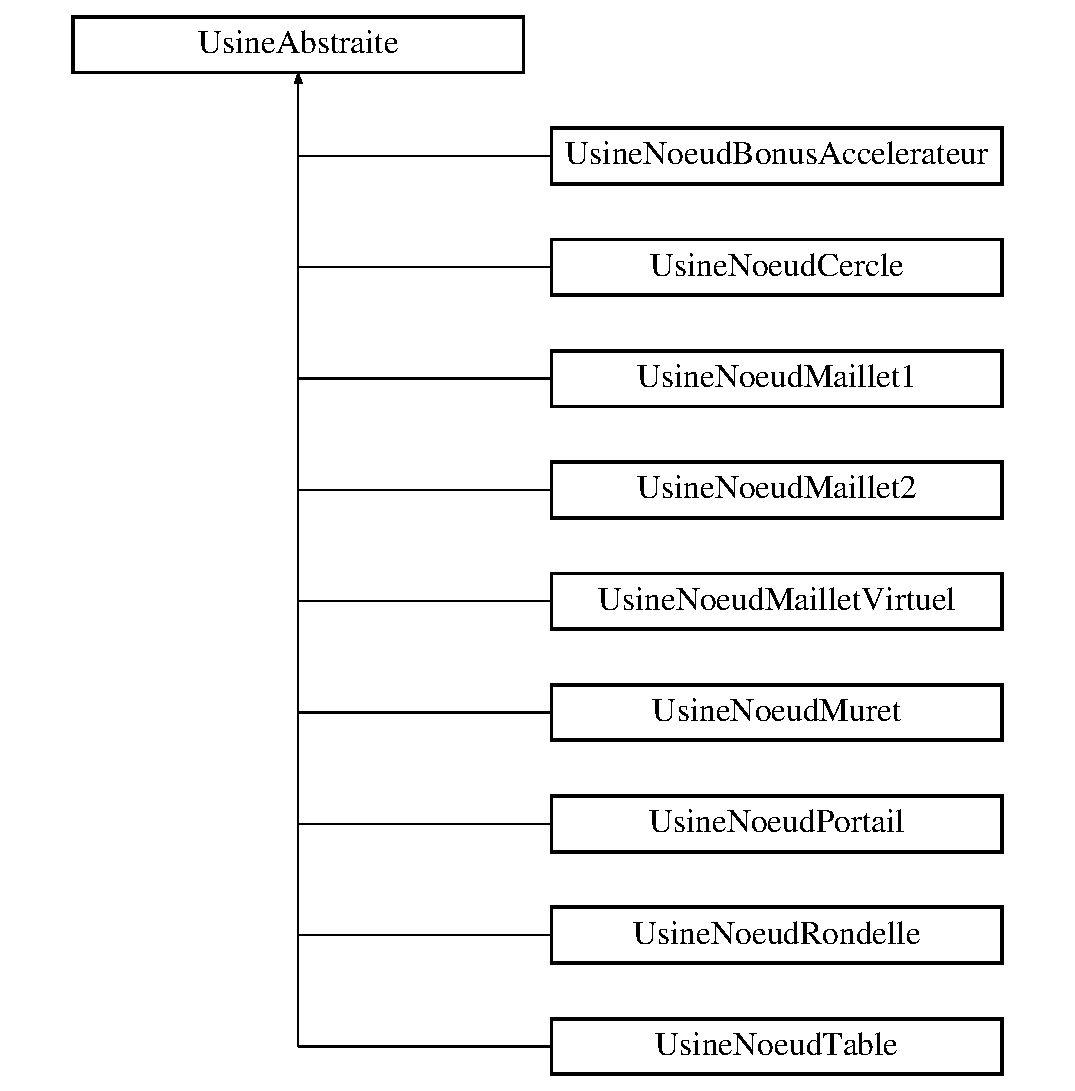
\includegraphics[height=0.812183cm]{class_usine_abstraite}
\end{center}
\end{figure}
\subsection*{Public Member Functions}
\begin{DoxyCompactItemize}
\item 
virtual \hyperlink{class_noeud_abstrait}{Noeud\+Abstrait} $\ast$ \hyperlink{group__inf2990_ga4e583ec371cef6ddb9a22dd23d232a2d}{creer\+Noeud} () const
\begin{DoxyCompactList}\small\item\em Fonction de cr�ation de noeud � surcharger. \end{DoxyCompactList}\item 
virtual \hyperlink{class_noeud_abstrait}{Noeud\+Abstrait} $\ast$ \hyperlink{group__inf2990_gac2a9e4abe1291b31d5e07d55edb7e02b}{creer\+Noeud} (tinyxml2\+::\+X\+M\+L\+Node $\ast$node) const
\begin{DoxyCompactList}\small\item\em Fonction de cr�ation de noeud � partir d\textquotesingle{}un noeud X\+ML � surcharger. \end{DoxyCompactList}\item 
\hypertarget{class_usine_abstraite_a21561b178ecd2af6f24ff60ea0bc3669}{}\label{class_usine_abstraite_a21561b178ecd2af6f24ff60ea0bc3669} 
{\bfseries Usine\+Abstraite} (const std\+::string \&nom\+Usine, const std\+::string \&nom\+Modele)
\end{DoxyCompactItemize}
\subsection*{Protected Member Functions}
\begin{DoxyCompactItemize}
\item 
\hypertarget{class_usine_abstraite_a6a5dc32968aa9a7ddd052c2b8f694447}{}\label{class_usine_abstraite_a6a5dc32968aa9a7ddd052c2b8f694447} 
{\bfseries Usine\+Abstraite} (std\+::string nom)
\item 
const std\+::string \& \hyperlink{group__inf2990_gab72c2ffc78376010142e9e31e8ab53f8}{obtenir\+Nom} () const
\begin{DoxyCompactList}\small\item\em Retourne le nom associ� � l\textquotesingle{}usine. \end{DoxyCompactList}\end{DoxyCompactItemize}
\subsection*{Protected Attributes}
\begin{DoxyCompactItemize}
\item 
\hypertarget{class_usine_abstraite_a082cf4d6129875f1c84fccb95db77cdf}{}\label{class_usine_abstraite_a082cf4d6129875f1c84fccb95db77cdf} 
modele\+::\+Modele3D {\bfseries modele\+\_\+}
\item 
\hypertarget{class_usine_abstraite_a45baf4d4ac1cd41851163625f1c601a1}{}\label{class_usine_abstraite_a45baf4d4ac1cd41851163625f1c601a1} 
opengl\+::\+V\+BO {\bfseries vbo\+\_\+}
\end{DoxyCompactItemize}


\subsection{Detailed Description}
Classe de base abstraite des usines qui seront utilis�es pour cr�er les diff�rents noeuds de l\textquotesingle{}arbre de rendu. 

\begin{DoxyAuthor}{Author}
Martin Bisson 
\end{DoxyAuthor}
\begin{DoxyDate}{Date}
2001-\/01-\/28 
\end{DoxyDate}


The documentation for this class was generated from the following file\+:\begin{DoxyCompactItemize}
\item 
Sources/\+D\+L\+L/\+Arbre/\+Usines/\hyperlink{_usine_noeud_8h}{Usine\+Noeud.\+h}\end{DoxyCompactItemize}

\hypertarget{class_usine_noeud_bonus_accelerateur}{}\section{Usine\+Noeud\+Bonus\+Accelerateur Class Reference}
\label{class_usine_noeud_bonus_accelerateur}\index{Usine\+Noeud\+Bonus\+Accelerateur@{Usine\+Noeud\+Bonus\+Accelerateur}}
Inheritance diagram for Usine\+Noeud\+Bonus\+Accelerateur\+:\begin{figure}[H]
\begin{center}
\leavevmode
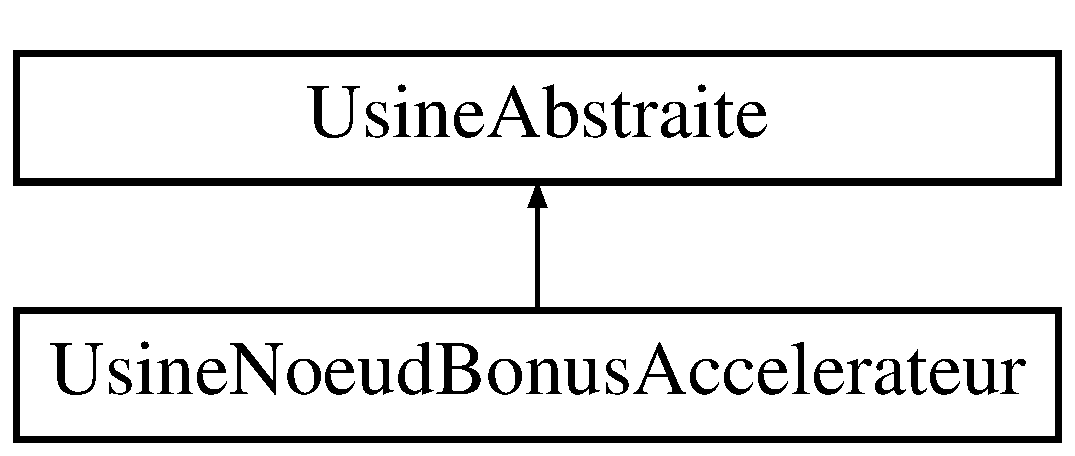
\includegraphics[height=2.000000cm]{class_usine_noeud_bonus_accelerateur}
\end{center}
\end{figure}
\subsection*{Public Member Functions}
\begin{DoxyCompactItemize}
\item 
\hyperlink{group__inf2990_ga71a45e8885f4a8b194f6398e9f1cef7b}{Usine\+Noeud\+Bonus\+Accelerateur} (const std\+::string \&nom)
\begin{DoxyCompactList}\small\item\em Constructeur par param�tres. \end{DoxyCompactList}\item 
virtual \hyperlink{class_noeud_abstrait}{Noeud\+Abstrait} $\ast$ \hyperlink{group__inf2990_ga5de51d6d3c79b62248dee720a462703d}{creer\+Noeud} () const
\begin{DoxyCompactList}\small\item\em Fonction pour cr�er un noeud. \end{DoxyCompactList}\item 
virtual \hyperlink{class_noeud_abstrait}{Noeud\+Abstrait} $\ast$ \hyperlink{group__inf2990_gabac8bc6332015f74bad38ed0b8d062a9}{creer\+Noeud} (tinyxml2\+::\+X\+M\+L\+Node $\ast$node) const
\begin{DoxyCompactList}\small\item\em Fonction pour cr�er un noeud � partir d\textquotesingle{}un noeud X\+ML. \end{DoxyCompactList}\end{DoxyCompactItemize}
\subsection*{Protected Attributes}
\begin{DoxyCompactItemize}
\item 
modele\+::\+Modele3D \hyperlink{group__inf2990_gade31611c0444efdd00cb60e5f6b636c4}{modele\+\_\+}
\begin{DoxyCompactList}\small\item\em Mod�le 3D correspondant � ce noeud. \end{DoxyCompactList}\item 
opengl\+::\+V\+BO \hyperlink{group__inf2990_ga4a71ed77e29b6867f42cc5db2a406a86}{vbo\+\_\+}
\begin{DoxyCompactList}\small\item\em Storage pour le dessin du mod�le. \end{DoxyCompactList}\end{DoxyCompactItemize}
\subsection*{Additional Inherited Members}


The documentation for this class was generated from the following file\+:\begin{DoxyCompactItemize}
\item 
Sources/\+D\+L\+L/\+Arbre/\+Usines/Usine\+Noeud\+Bonus\+Accelerateur.\+h\end{DoxyCompactItemize}

\hypertarget{class_usine_noeud_cercle}{}\section{Usine\+Noeud\+Cercle Class Reference}
\label{class_usine_noeud_cercle}\index{Usine\+Noeud\+Cercle@{Usine\+Noeud\+Cercle}}
Inheritance diagram for Usine\+Noeud\+Cercle\+:\begin{figure}[H]
\begin{center}
\leavevmode
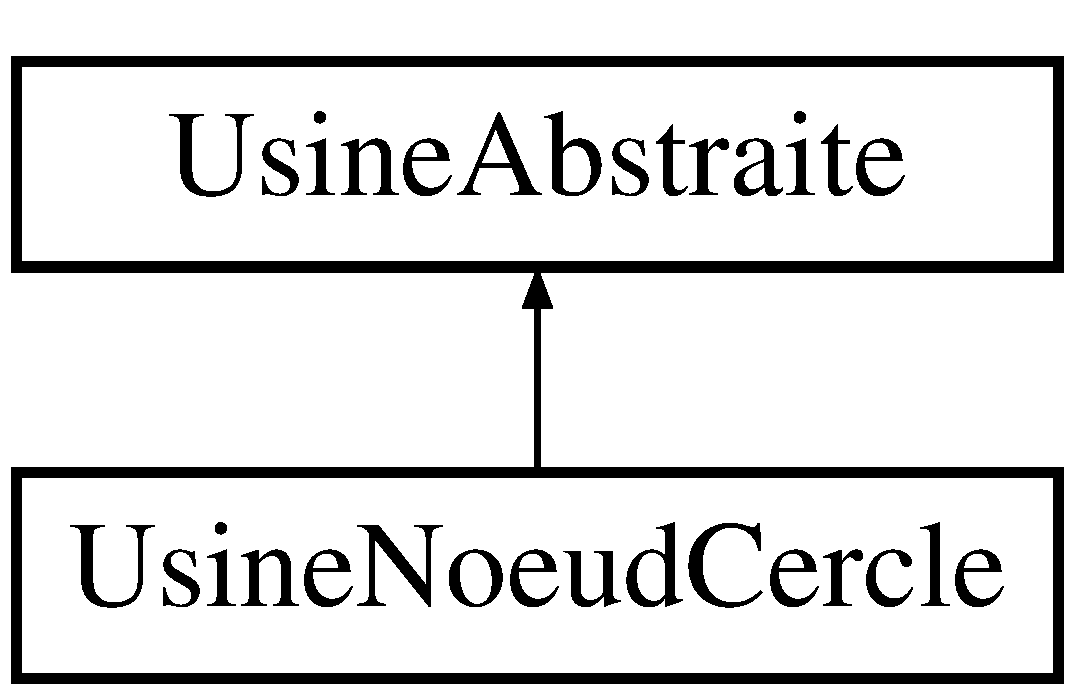
\includegraphics[height=2.000000cm]{class_usine_noeud_cercle}
\end{center}
\end{figure}
\subsection*{Public Member Functions}
\begin{DoxyCompactItemize}
\item 
\hyperlink{group__inf2990_ga00c5b0af1f007124e0f1fa0ab58f339a}{Usine\+Noeud\+Cercle} (const std\+::string \&nom)
\begin{DoxyCompactList}\small\item\em Constructeur par param�tres. \end{DoxyCompactList}\item 
virtual \hyperlink{class_noeud_abstrait}{Noeud\+Abstrait} $\ast$ \hyperlink{group__inf2990_gaa341e0b93614b9c7258ebd11b1aad5ce}{creer\+Noeud} () const
\begin{DoxyCompactList}\small\item\em Fonction pour cr�er un noeud. \end{DoxyCompactList}\item 
virtual \hyperlink{class_noeud_abstrait}{Noeud\+Abstrait} $\ast$ \hyperlink{group__inf2990_gafe9c3e3267b59b56ead91820e8367a9f}{creer\+Noeud} (tinyxml2\+::\+X\+M\+L\+Node $\ast$node) const
\begin{DoxyCompactList}\small\item\em Fonction pour cr�er un noeud � partir d\textquotesingle{}un noeud X\+ML. \end{DoxyCompactList}\end{DoxyCompactItemize}
\subsection*{Protected Attributes}
\begin{DoxyCompactItemize}
\item 
modele\+::\+Modele3D \hyperlink{group__inf2990_ga1249da475160c157d796014ea891432c}{modele\+\_\+}
\begin{DoxyCompactList}\small\item\em Mod�le 3D correspondant � ce noeud. \end{DoxyCompactList}\item 
opengl\+::\+V\+BO \hyperlink{group__inf2990_ga182a5f272094457c0be02fbeadc23700}{vbo\+\_\+}
\begin{DoxyCompactList}\small\item\em Storage pour le dessin du mod�le. \end{DoxyCompactList}\end{DoxyCompactItemize}
\subsection*{Additional Inherited Members}


The documentation for this class was generated from the following file\+:\begin{DoxyCompactItemize}
\item 
Sources/\+D\+L\+L/\+Arbre/\+Usines/Usine\+Noeud\+Cercle.\+h\end{DoxyCompactItemize}

\hypertarget{class_usine_noeud_maillet}{}\section{Usine\+Noeud\+Maillet Class Reference}
\label{class_usine_noeud_maillet}\index{Usine\+Noeud\+Maillet@{Usine\+Noeud\+Maillet}}


Classe qui repr�sente une usine capable de cr�er des noeuds de type \hyperlink{class_noeud_portail}{Noeud\+Portail}.  




{\ttfamily \#include $<$Usine\+Noeud\+Maillet1.\+h$>$}



\subsection{Detailed Description}
Classe qui repr�sente une usine capable de cr�er des noeuds de type \hyperlink{class_noeud_portail}{Noeud\+Portail}. 

\begin{DoxyAuthor}{Author}
Equipe06 
\end{DoxyAuthor}
\begin{DoxyDate}{Date}
2016-\/09-\/30 
\end{DoxyDate}


The documentation for this class was generated from the following file\+:\begin{DoxyCompactItemize}
\item 
Sources/\+D\+L\+L/\+Arbre/\+Usines/Usine\+Noeud\+Maillet1.\+h\end{DoxyCompactItemize}

\hypertarget{class_usine_noeud_maillet1}{}\section{Usine\+Noeud\+Maillet1 Class Reference}
\label{class_usine_noeud_maillet1}\index{Usine\+Noeud\+Maillet1@{Usine\+Noeud\+Maillet1}}
Inheritance diagram for Usine\+Noeud\+Maillet1\+:\begin{figure}[H]
\begin{center}
\leavevmode
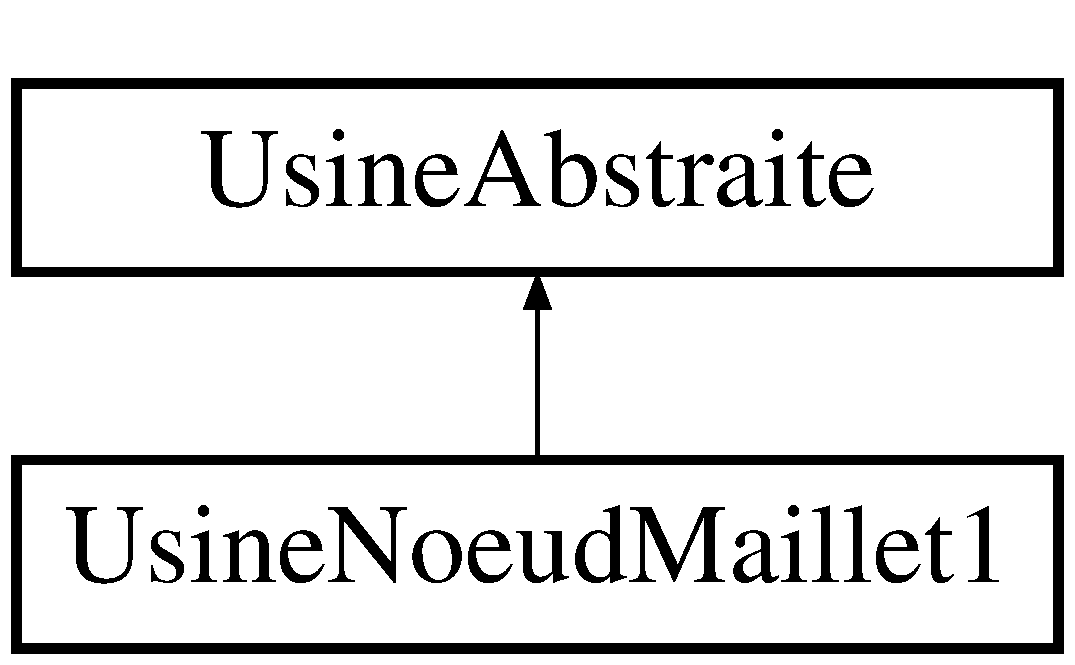
\includegraphics[height=2.000000cm]{class_usine_noeud_maillet1}
\end{center}
\end{figure}
\subsection*{Public Member Functions}
\begin{DoxyCompactItemize}
\item 
\hyperlink{group__inf2990_ga0ab6fb7f88bb261545732e728c42986e}{Usine\+Noeud\+Maillet1} (const std\+::string \&nom)
\begin{DoxyCompactList}\small\item\em Constructeur par param�tres. \end{DoxyCompactList}\item 
virtual \hyperlink{class_noeud_abstrait}{Noeud\+Abstrait} $\ast$ \hyperlink{group__inf2990_ga31fafa64fe928607d3b29dfbff39a543}{creer\+Noeud} () const
\begin{DoxyCompactList}\small\item\em Fonction pour cr�er un noeud. \end{DoxyCompactList}\item 
virtual \hyperlink{class_noeud_abstrait}{Noeud\+Abstrait} $\ast$ \hyperlink{group__inf2990_gab5cedeb3600b168765e7de1935986b24}{creer\+Noeud} (tinyxml2\+::\+X\+M\+L\+Node $\ast$node) const
\begin{DoxyCompactList}\small\item\em Fonction pour cr�er un noeud � partir d\textquotesingle{}un noeud X\+ML. \end{DoxyCompactList}\end{DoxyCompactItemize}
\subsection*{Protected Attributes}
\begin{DoxyCompactItemize}
\item 
modele\+::\+Modele3D \hyperlink{group__inf2990_gac30c6d2c003996917f2cec9756994029}{modele\+\_\+}
\begin{DoxyCompactList}\small\item\em Mod�le 3D correspondant � ce noeud. \end{DoxyCompactList}\item 
opengl\+::\+V\+BO \hyperlink{group__inf2990_ga9a131e72976f88ee8f63c6b42afc3b7a}{vbo\+\_\+}
\begin{DoxyCompactList}\small\item\em Storage pour le dessin du mod�le. \end{DoxyCompactList}\end{DoxyCompactItemize}
\subsection*{Additional Inherited Members}


The documentation for this class was generated from the following file\+:\begin{DoxyCompactItemize}
\item 
C\+:/\+Users/\+Steven/\+Documents/\+Poly/\+I\+N\+F2990/inf2990-\/06/\+Cadriciel\+\_\+2016-\/3\+\_\+\+Etudiants/\+Cadriciel/\+Sources/\+D\+L\+L/\+Arbre/\+Usines/Usine\+Noeud\+Maillet1.\+h\end{DoxyCompactItemize}

\hypertarget{class_usine_noeud_maillet2}{}\section{Usine\+Noeud\+Maillet2 Class Reference}
\label{class_usine_noeud_maillet2}\index{Usine\+Noeud\+Maillet2@{Usine\+Noeud\+Maillet2}}
Inheritance diagram for Usine\+Noeud\+Maillet2\+:\begin{figure}[H]
\begin{center}
\leavevmode
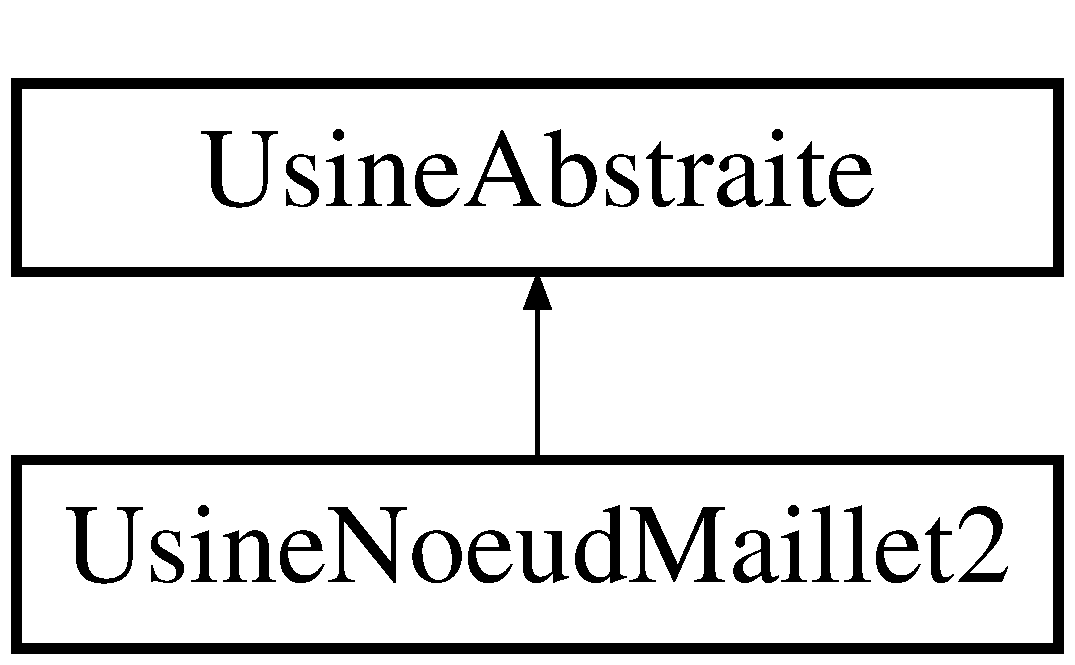
\includegraphics[height=2.000000cm]{class_usine_noeud_maillet2}
\end{center}
\end{figure}
\subsection*{Public Member Functions}
\begin{DoxyCompactItemize}
\item 
\hyperlink{group__inf2990_gadac324f619065183d7a0552c134f18b6}{Usine\+Noeud\+Maillet2} (const std\+::string \&nom)
\begin{DoxyCompactList}\small\item\em Constructeur par param�tres. \end{DoxyCompactList}\item 
virtual \hyperlink{class_noeud_abstrait}{Noeud\+Abstrait} $\ast$ \hyperlink{group__inf2990_gad2fdf620b0dbc1dd82465e7c106e8868}{creer\+Noeud} () const
\begin{DoxyCompactList}\small\item\em Fonction pour cr�er un noeud. \end{DoxyCompactList}\item 
virtual \hyperlink{class_noeud_abstrait}{Noeud\+Abstrait} $\ast$ \hyperlink{group__inf2990_ga900e6aecccbf0073445ff744a46256cb}{creer\+Noeud} (tinyxml2\+::\+X\+M\+L\+Node $\ast$node) const
\begin{DoxyCompactList}\small\item\em Fonction pour cr�er un noeud � partir d\textquotesingle{}un noeud X\+ML. \end{DoxyCompactList}\end{DoxyCompactItemize}
\subsection*{Protected Attributes}
\begin{DoxyCompactItemize}
\item 
modele\+::\+Modele3D \hyperlink{group__inf2990_gafd1ef201420ccfc7e6d47c897a932770}{modele\+\_\+}
\begin{DoxyCompactList}\small\item\em Mod�le 3D correspondant � ce noeud. \end{DoxyCompactList}\item 
opengl\+::\+V\+BO \hyperlink{group__inf2990_ga8327e4ed6a382f0705cff133ed7fc776}{vbo\+\_\+}
\begin{DoxyCompactList}\small\item\em Storage pour le dessin du mod�le. \end{DoxyCompactList}\end{DoxyCompactItemize}
\subsection*{Additional Inherited Members}


The documentation for this class was generated from the following file\+:\begin{DoxyCompactItemize}
\item 
Sources/\+D\+L\+L/Usine\+Noeud\+Maillet2.\+h\end{DoxyCompactItemize}

\hypertarget{class_usine_noeud_maillet_virtuel}{}\section{Usine\+Noeud\+Maillet\+Virtuel Class Reference}
\label{class_usine_noeud_maillet_virtuel}\index{Usine\+Noeud\+Maillet\+Virtuel@{Usine\+Noeud\+Maillet\+Virtuel}}
Inheritance diagram for Usine\+Noeud\+Maillet\+Virtuel\+:\begin{figure}[H]
\begin{center}
\leavevmode
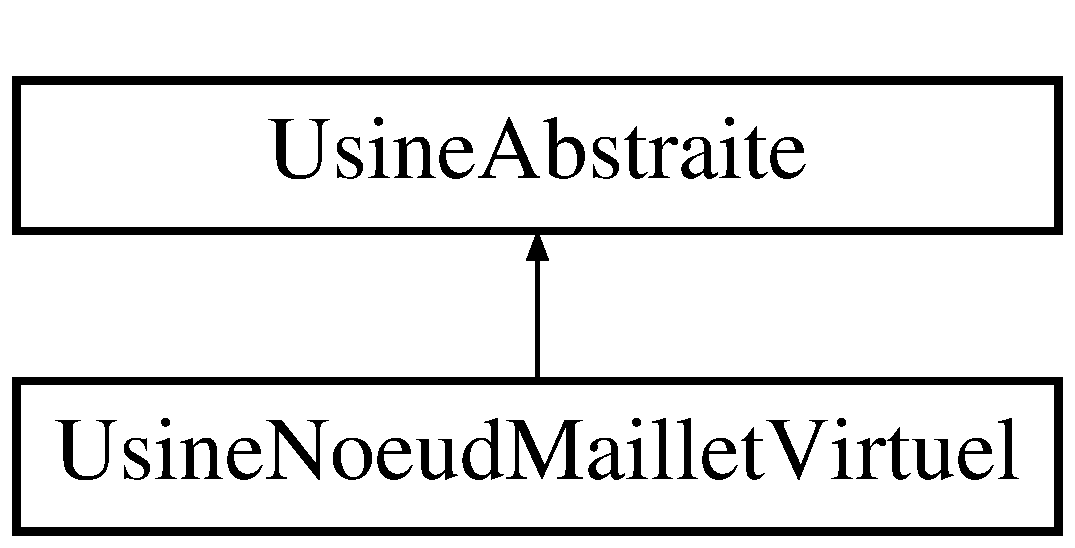
\includegraphics[height=2.000000cm]{class_usine_noeud_maillet_virtuel}
\end{center}
\end{figure}
\subsection*{Public Member Functions}
\begin{DoxyCompactItemize}
\item 
\hyperlink{group__inf2990_ga19c09f5497973c6d5c1ec9fc5122e210}{Usine\+Noeud\+Maillet\+Virtuel} (const std\+::string \&nom)
\begin{DoxyCompactList}\small\item\em Constructeur par param�tres. \end{DoxyCompactList}\item 
virtual \hyperlink{class_noeud_abstrait}{Noeud\+Abstrait} $\ast$ \hyperlink{group__inf2990_ga30033fa4215fc284d24ee1d893830ce4}{creer\+Noeud} () const
\begin{DoxyCompactList}\small\item\em Fonction pour cr�er un noeud. \end{DoxyCompactList}\item 
virtual \hyperlink{class_noeud_abstrait}{Noeud\+Abstrait} $\ast$ \hyperlink{group__inf2990_ga101993b32ee79640cd2b3ba5c2991605}{creer\+Noeud} (tinyxml2\+::\+X\+M\+L\+Node $\ast$node) const
\begin{DoxyCompactList}\small\item\em Fonction pour cr�er un noeud � partir d\textquotesingle{}un noeud X\+ML. \end{DoxyCompactList}\end{DoxyCompactItemize}
\subsection*{Protected Attributes}
\begin{DoxyCompactItemize}
\item 
modele\+::\+Modele3D \hyperlink{group__inf2990_ga8cab3e9e00a2d3ce8410ee3020657a1e}{modele\+\_\+}
\begin{DoxyCompactList}\small\item\em Mod�le 3D correspondant � ce noeud. \end{DoxyCompactList}\item 
opengl\+::\+V\+BO \hyperlink{group__inf2990_gac6c44daeca526ac59ab903b4591ba040}{vbo\+\_\+}
\begin{DoxyCompactList}\small\item\em Storage pour le dessin du mod�le. \end{DoxyCompactList}\end{DoxyCompactItemize}
\subsection*{Additional Inherited Members}


The documentation for this class was generated from the following file\+:\begin{DoxyCompactItemize}
\item 
Sources/\+D\+L\+L/\+Arbre/\+Usines/Usine\+Noeud\+Maillet\+Virtuel.\+h\end{DoxyCompactItemize}

\hypertarget{class_usine_noeud_muret}{}\section{Usine\+Noeud\+Muret Class Reference}
\label{class_usine_noeud_muret}\index{Usine\+Noeud\+Muret@{Usine\+Noeud\+Muret}}
Inheritance diagram for Usine\+Noeud\+Muret\+:\begin{figure}[H]
\begin{center}
\leavevmode
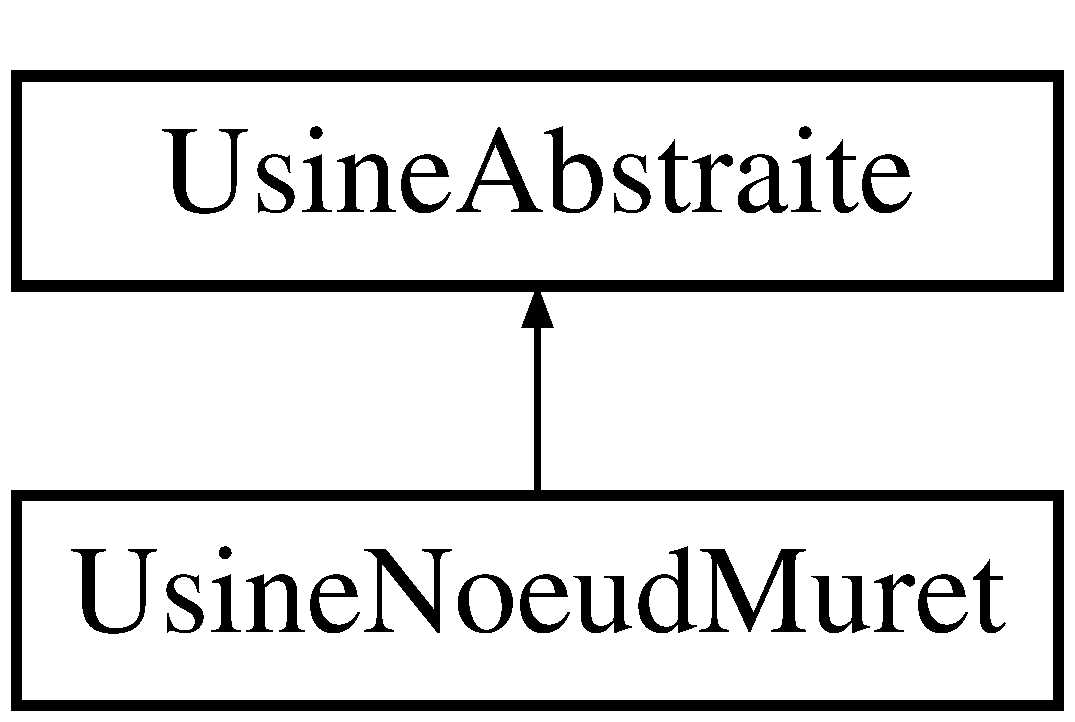
\includegraphics[height=2.000000cm]{class_usine_noeud_muret}
\end{center}
\end{figure}
\subsection*{Public Member Functions}
\begin{DoxyCompactItemize}
\item 
\hyperlink{group__inf2990_gaa2b942ea7c1464c37c79faccabc6b63d}{Usine\+Noeud\+Muret} (const std\+::string \&nom)
\begin{DoxyCompactList}\small\item\em Constructeur par param�tres. \end{DoxyCompactList}\item 
virtual \hyperlink{class_noeud_abstrait}{Noeud\+Abstrait} $\ast$ \hyperlink{group__inf2990_ga76e5422e92363d5344141c08fac1978c}{creer\+Noeud} () const
\begin{DoxyCompactList}\small\item\em Fonction pour cr�er un noeud. \end{DoxyCompactList}\item 
virtual \hyperlink{class_noeud_abstrait}{Noeud\+Abstrait} $\ast$ \hyperlink{group__inf2990_ga20539411f0f7c1333ea132c916499778}{creer\+Noeud} (tinyxml2\+::\+X\+M\+L\+Node $\ast$node) const
\begin{DoxyCompactList}\small\item\em Fonction pour cr�er un noeud � partir d\textquotesingle{}un noeud X\+ML. \end{DoxyCompactList}\end{DoxyCompactItemize}
\subsection*{Protected Attributes}
\begin{DoxyCompactItemize}
\item 
modele\+::\+Modele3D \hyperlink{group__inf2990_gacb003bc12d5150a4e8dafddde99898ca}{modele\+\_\+}
\begin{DoxyCompactList}\small\item\em Mod�le 3D correspondant � ce noeud. \end{DoxyCompactList}\item 
opengl\+::\+V\+BO \hyperlink{group__inf2990_gac82fb530a2b5bc302b3123af6012f603}{vbo\+\_\+}
\begin{DoxyCompactList}\small\item\em Storage pour le dessin du mod�le. \end{DoxyCompactList}\end{DoxyCompactItemize}
\subsection*{Additional Inherited Members}


The documentation for this class was generated from the following file\+:\begin{DoxyCompactItemize}
\item 
Sources/\+D\+L\+L/\+Arbre/\+Usines/Usine\+Noeud\+Muret.\+h\end{DoxyCompactItemize}

\hypertarget{class_usine_noeud_portail}{}\section{Usine\+Noeud\+Portail Class Reference}
\label{class_usine_noeud_portail}\index{Usine\+Noeud\+Portail@{Usine\+Noeud\+Portail}}


Classe qui repr�sente une usine capable de cr�er des noeuds de type \hyperlink{class_noeud_portail}{Noeud\+Portail}.  




{\ttfamily \#include $<$Usine\+Noeud\+Bonus\+Accelerateur.\+h$>$}

Inheritance diagram for Usine\+Noeud\+Portail\+:\begin{figure}[H]
\begin{center}
\leavevmode
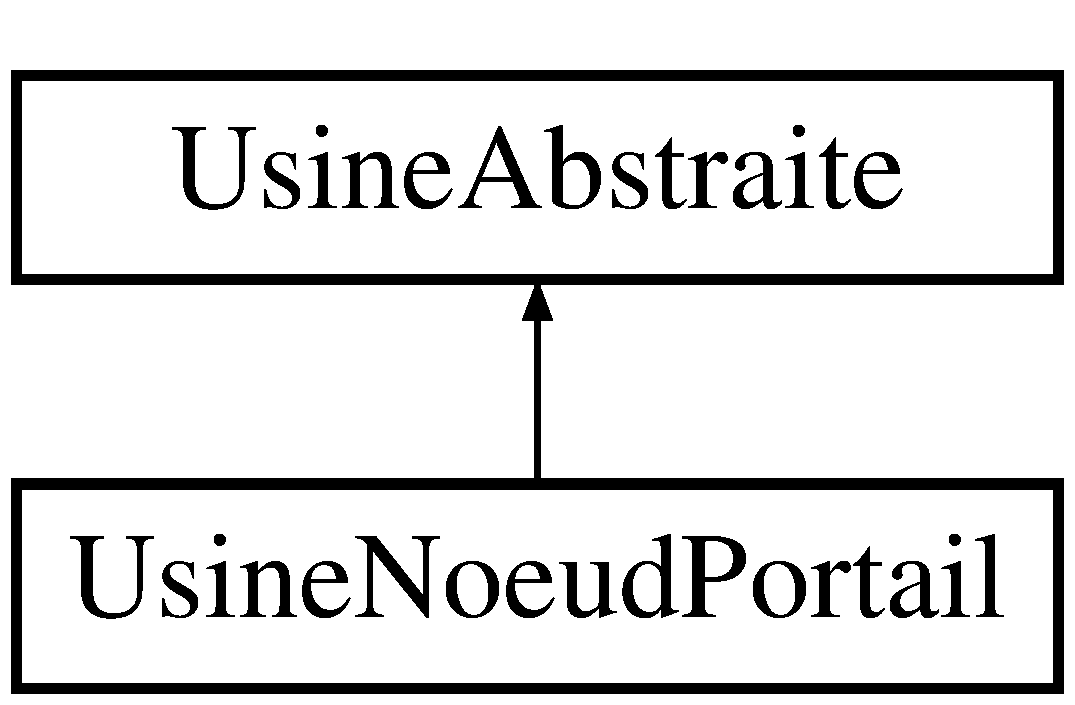
\includegraphics[height=2.000000cm]{class_usine_noeud_portail}
\end{center}
\end{figure}
\subsection*{Public Member Functions}
\begin{DoxyCompactItemize}
\item 
\hyperlink{group__inf2990_ga7d0e963f0f08f6f4544df420b9a747f4}{Usine\+Noeud\+Portail} (const std\+::string \&nom)
\begin{DoxyCompactList}\small\item\em Constructeur par param�tres. \end{DoxyCompactList}\item 
virtual \hyperlink{class_noeud_abstrait}{Noeud\+Abstrait} $\ast$ \hyperlink{group__inf2990_ga9da8c13351933b1ecac1e59cf04f266f}{creer\+Noeud} () const
\begin{DoxyCompactList}\small\item\em Fonction pour cr�er un noeud. \end{DoxyCompactList}\item 
virtual \hyperlink{class_noeud_abstrait}{Noeud\+Abstrait} $\ast$ \hyperlink{group__inf2990_ga9f4999f2b24c7794c6f6648e0ea18bec}{creer\+Noeud} (tinyxml2\+::\+X\+M\+L\+Node $\ast$node) const
\begin{DoxyCompactList}\small\item\em Fonction pour cr�er un noeud � partir d\textquotesingle{}un noeud X\+ML. \end{DoxyCompactList}\end{DoxyCompactItemize}
\subsection*{Protected Attributes}
\begin{DoxyCompactItemize}
\item 
modele\+::\+Modele3D \hyperlink{group__inf2990_gaa709032dc2c073276f3d22d160e6e9de}{modele\+\_\+}
\begin{DoxyCompactList}\small\item\em Mod�le 3D correspondant � ce noeud. \end{DoxyCompactList}\item 
opengl\+::\+V\+BO \hyperlink{group__inf2990_ga78efc1d00fab9cb6ec355dff34778d2e}{vbo\+\_\+}
\begin{DoxyCompactList}\small\item\em Storage pour le dessin du mod�le. \end{DoxyCompactList}\end{DoxyCompactItemize}
\subsection*{Additional Inherited Members}


\subsection{Detailed Description}
Classe qui repr�sente une usine capable de cr�er des noeuds de type \hyperlink{class_noeud_portail}{Noeud\+Portail}. 

\begin{DoxyAuthor}{Author}
Equipe06 
\end{DoxyAuthor}
\begin{DoxyDate}{Date}
2016-\/09-\/30 
\end{DoxyDate}


The documentation for this class was generated from the following file\+:\begin{DoxyCompactItemize}
\item 
Sources/\+D\+L\+L/\+Arbre/\+Usines/\hyperlink{_usine_noeud_portail_8h}{Usine\+Noeud\+Portail.\+h}\end{DoxyCompactItemize}

\hypertarget{class_usine_noeud_rondelle}{}\section{Usine\+Noeud\+Rondelle Class Reference}
\label{class_usine_noeud_rondelle}\index{Usine\+Noeud\+Rondelle@{Usine\+Noeud\+Rondelle}}
Inheritance diagram for Usine\+Noeud\+Rondelle\+:\begin{figure}[H]
\begin{center}
\leavevmode
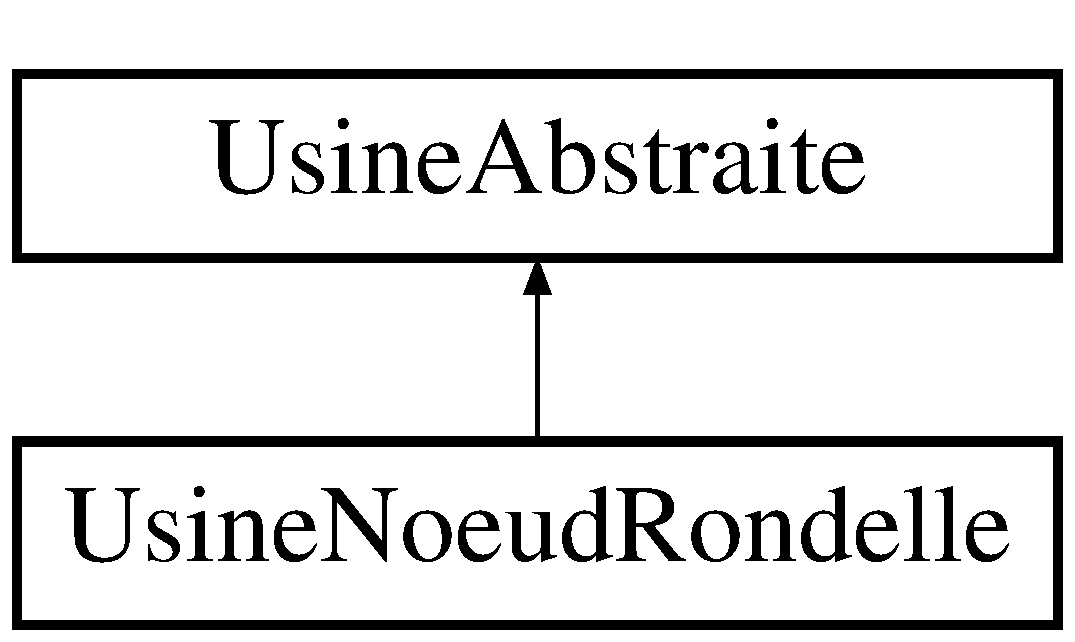
\includegraphics[height=2.000000cm]{class_usine_noeud_rondelle}
\end{center}
\end{figure}
\subsection*{Public Member Functions}
\begin{DoxyCompactItemize}
\item 
\hyperlink{group__inf2990_ga3b82cbcc3f2be5e39dde1a200e7ad4b1}{Usine\+Noeud\+Rondelle} (const std\+::string \&nom)
\begin{DoxyCompactList}\small\item\em Constructeur par param�tres. \end{DoxyCompactList}\item 
virtual \hyperlink{class_noeud_abstrait}{Noeud\+Abstrait} $\ast$ \hyperlink{group__inf2990_gab5360352a80843940bd6936b93b67b38}{creer\+Noeud} () const
\begin{DoxyCompactList}\small\item\em Fonction pour cr�er un noeud. \end{DoxyCompactList}\item 
virtual \hyperlink{class_noeud_abstrait}{Noeud\+Abstrait} $\ast$ \hyperlink{group__inf2990_ga4654cb3c3a7972f3bcbb090dfff47aa6}{creer\+Noeud} (tinyxml2\+::\+X\+M\+L\+Node $\ast$node) const
\begin{DoxyCompactList}\small\item\em Fonction pour cr�er un noeud � partir d\textquotesingle{}un noeud X\+ML. \end{DoxyCompactList}\end{DoxyCompactItemize}
\subsection*{Protected Attributes}
\begin{DoxyCompactItemize}
\item 
modele\+::\+Modele3D \hyperlink{group__inf2990_gab18a707f615fa48974722604087ed18d}{modele\+\_\+}
\begin{DoxyCompactList}\small\item\em Mod�le 3D correspondant � ce noeud. \end{DoxyCompactList}\item 
opengl\+::\+V\+BO \hyperlink{group__inf2990_gafbdedb988270e0496c62a3cea8bfbb39}{vbo\+\_\+}
\begin{DoxyCompactList}\small\item\em Storage pour le dessin du mod�le. \end{DoxyCompactList}\end{DoxyCompactItemize}
\subsection*{Additional Inherited Members}


The documentation for this class was generated from the following file\+:\begin{DoxyCompactItemize}
\item 
C\+:/\+Users/\+Steven/\+Documents/\+Poly/\+I\+N\+F2990/inf2990-\/06/\+Cadriciel\+\_\+2016-\/3\+\_\+\+Etudiants/\+Cadriciel/\+Sources/\+D\+L\+L/\+Arbre/\+Usines/Usine\+Noeud\+Rondelle.\+h\end{DoxyCompactItemize}

\hypertarget{class_usine_noeud_table}{}\section{Usine\+Noeud\+Table Class Reference}
\label{class_usine_noeud_table}\index{Usine\+Noeud\+Table@{Usine\+Noeud\+Table}}
Inheritance diagram for Usine\+Noeud\+Table\+:\begin{figure}[H]
\begin{center}
\leavevmode
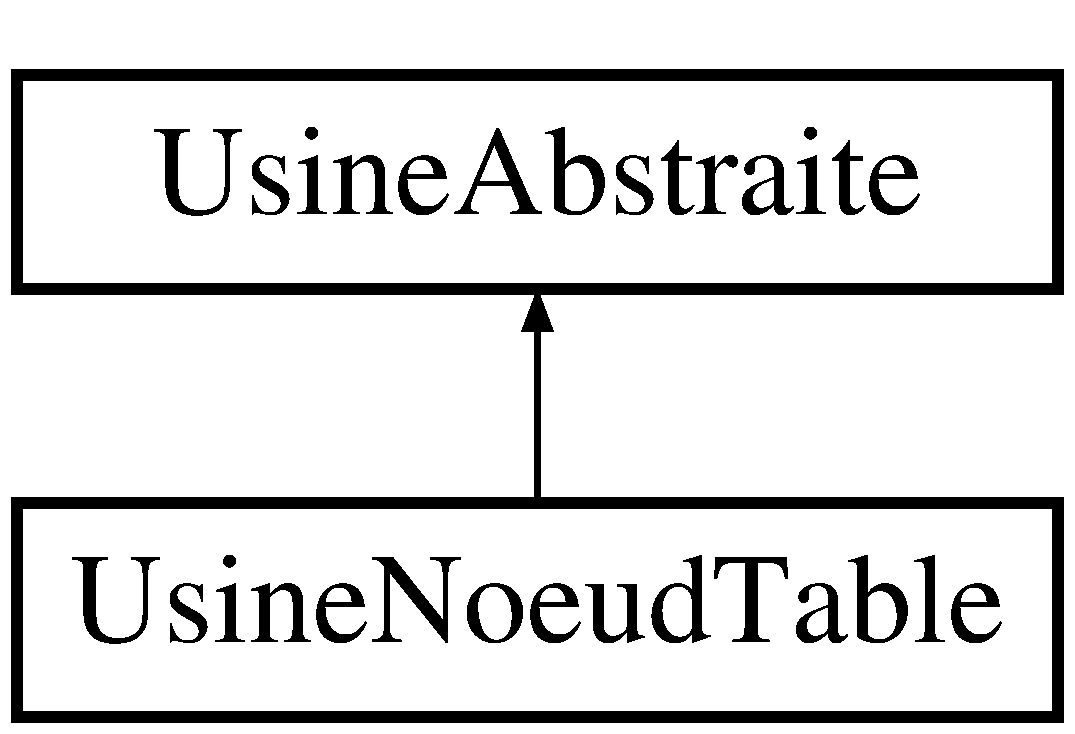
\includegraphics[height=2.000000cm]{class_usine_noeud_table}
\end{center}
\end{figure}
\subsection*{Public Member Functions}
\begin{DoxyCompactItemize}
\item 
\hyperlink{group__inf2990_ga90e6bb9138639f52de7129a06d8fc1ab}{Usine\+Noeud\+Table} (const std\+::string \&nom)
\begin{DoxyCompactList}\small\item\em Constructeur par param�tres. \end{DoxyCompactList}\item 
virtual \hyperlink{class_noeud_abstrait}{Noeud\+Abstrait} $\ast$ \hyperlink{group__inf2990_ga35c839c2fd6be3afa4e53a5bedc5851e}{creer\+Noeud} () const
\begin{DoxyCompactList}\small\item\em Fonction pour cr�er un noeud. \end{DoxyCompactList}\item 
virtual \hyperlink{class_noeud_abstrait}{Noeud\+Abstrait} $\ast$ \hyperlink{group__inf2990_ga8cd127d3f5062641c29b867a71f2237f}{creer\+Noeud} (tinyxml2\+::\+X\+M\+L\+Node $\ast$node) const
\begin{DoxyCompactList}\small\item\em Fonction pour cr�er un noeud � partir d\textquotesingle{}un noeud X\+ML. \end{DoxyCompactList}\end{DoxyCompactItemize}
\subsection*{Protected Attributes}
\begin{DoxyCompactItemize}
\item 
modele\+::\+Modele3D \hyperlink{group__inf2990_ga1803e63d30d1c1a6604c417f26d85bc4}{modele\+\_\+}
\begin{DoxyCompactList}\small\item\em Mod�le 3D correspondant � ce noeud. \end{DoxyCompactList}\item 
opengl\+::\+V\+BO \hyperlink{group__inf2990_ga7c06613487e5de3e6d0bb39e5130a112}{vbo\+\_\+}
\begin{DoxyCompactList}\small\item\em Storage pour le dessin du mod�le. \end{DoxyCompactList}\end{DoxyCompactItemize}
\subsection*{Additional Inherited Members}


The documentation for this class was generated from the following file\+:\begin{DoxyCompactItemize}
\item 
C\+:/\+Users/\+Steven/\+Documents/\+Poly/\+I\+N\+F2990/inf2990-\/06/\+Cadriciel\+\_\+2016-\/3\+\_\+\+Etudiants/\+Cadriciel/\+Sources/\+D\+L\+L/\+Arbre/\+Usines/\hyperlink{_usine_noeud_table_8h}{Usine\+Noeud\+Table.\+h}\end{DoxyCompactItemize}

\hypertarget{class_visiteur_abstrait}{}\section{Visiteur\+Abstrait Class Reference}
\label{class_visiteur_abstrait}\index{Visiteur\+Abstrait@{Visiteur\+Abstrait}}
Inheritance diagram for Visiteur\+Abstrait\+:\begin{figure}[H]
\begin{center}
\leavevmode
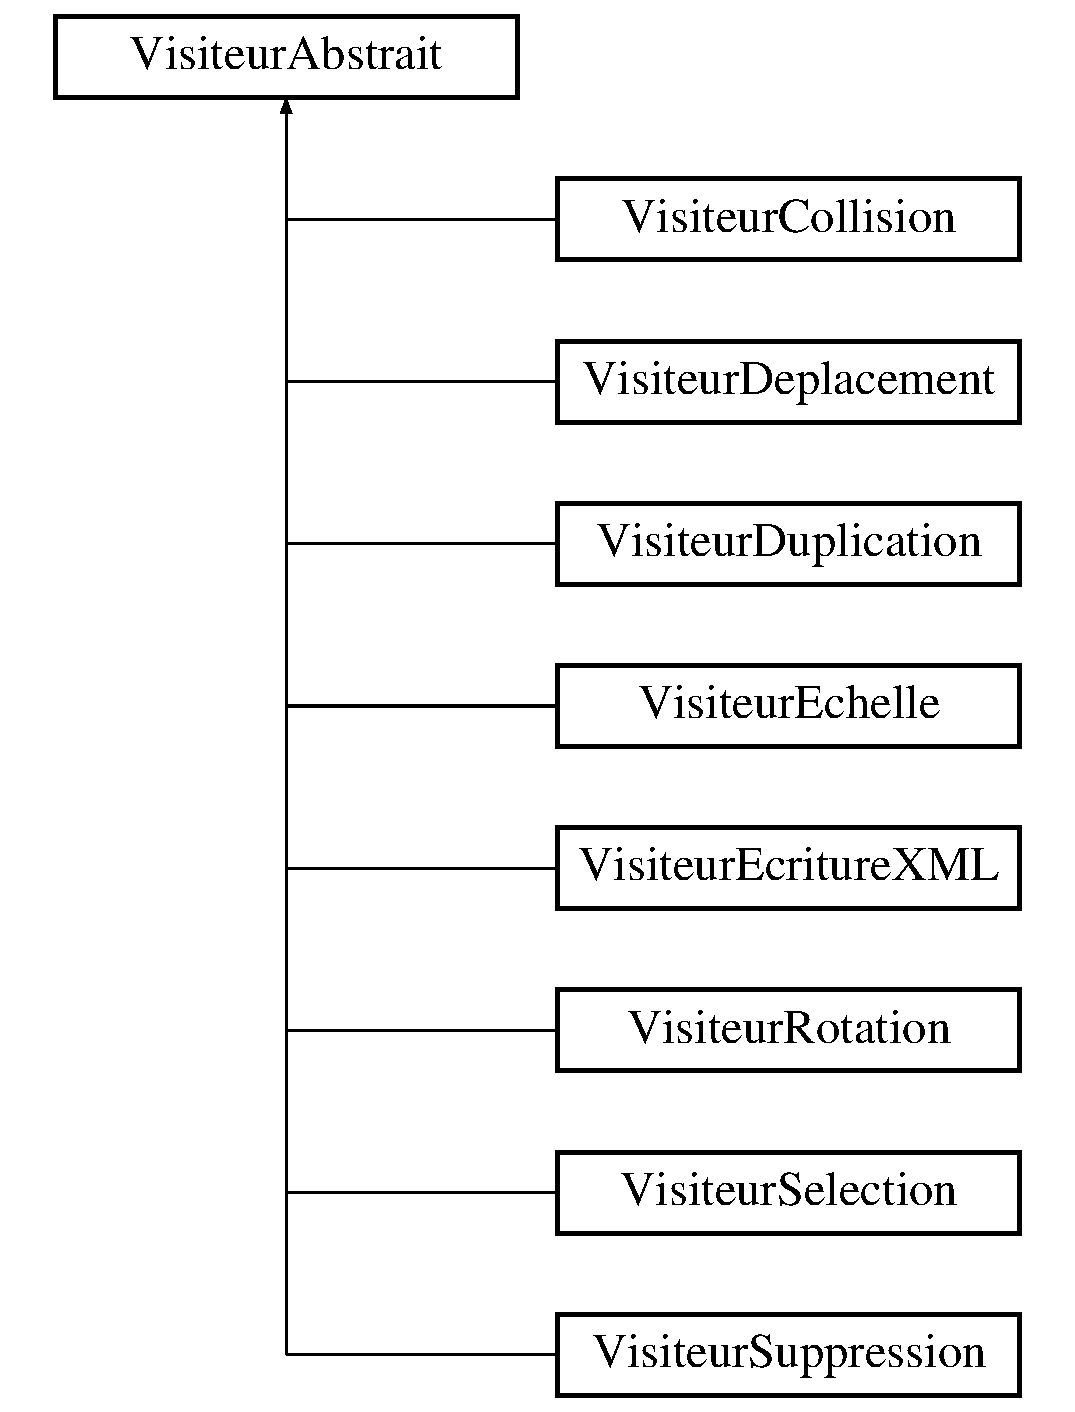
\includegraphics[height=9.000000cm]{class_visiteur_abstrait}
\end{center}
\end{figure}
\subsection*{Public Member Functions}
\begin{DoxyCompactItemize}
\item 
\hyperlink{group__inf2990_gab30d8c699bab1b4538f79e5750468d2d}{Visiteur\+Abstrait} ()
\begin{DoxyCompactList}\small\item\em Visiteur. \end{DoxyCompactList}\item 
virtual void {\bfseries visiter} (\hyperlink{class_noeud_composite}{Noeud\+Composite} $\ast$noeud)
\item 
virtual void {\bfseries visiter} (\hyperlink{class_noeud_maillet}{Noeud\+Maillet} $\ast$noeud)
\item 
virtual void {\bfseries visiter} (\hyperlink{class_noeud_muret}{Noeud\+Muret} $\ast$noeud)
\item 
virtual void {\bfseries visiter} (\hyperlink{class_noeud_portail}{Noeud\+Portail} $\ast$noeud)
\item 
virtual void {\bfseries visiter} (\hyperlink{class_noeud_rondelle}{Noeud\+Rondelle} $\ast$noeud)
\item 
virtual void {\bfseries visiter} (\hyperlink{class_noeud_table}{Noeud\+Table} $\ast$noeud)
\item 
virtual void {\bfseries visiter} (\hyperlink{class_noeud_bonus_accelerateur}{Noeud\+Bonus\+Accelerateur} $\ast$noeud)
\item 
virtual void {\bfseries visiter} (\hyperlink{class_noeud_maillet_virtuel}{Noeud\+Maillet\+Virtuel} $\ast$noeud)
\end{DoxyCompactItemize}
\subsection*{Protected Attributes}
\begin{DoxyCompactItemize}
\item 
std\+::string {\bfseries type\+\_\+}
\end{DoxyCompactItemize}


The documentation for this class was generated from the following file\+:\begin{DoxyCompactItemize}
\item 
Sources/\+D\+L\+L/\hyperlink{_visiteur_abstrait_8h}{Visiteur\+Abstrait.\+h}\end{DoxyCompactItemize}

\hypertarget{class_visiteur_collision}{}\section{Visiteur\+Collision Class Reference}
\label{class_visiteur_collision}\index{Visiteur\+Collision@{Visiteur\+Collision}}
Inheritance diagram for Visiteur\+Collision\+:\begin{figure}[H]
\begin{center}
\leavevmode
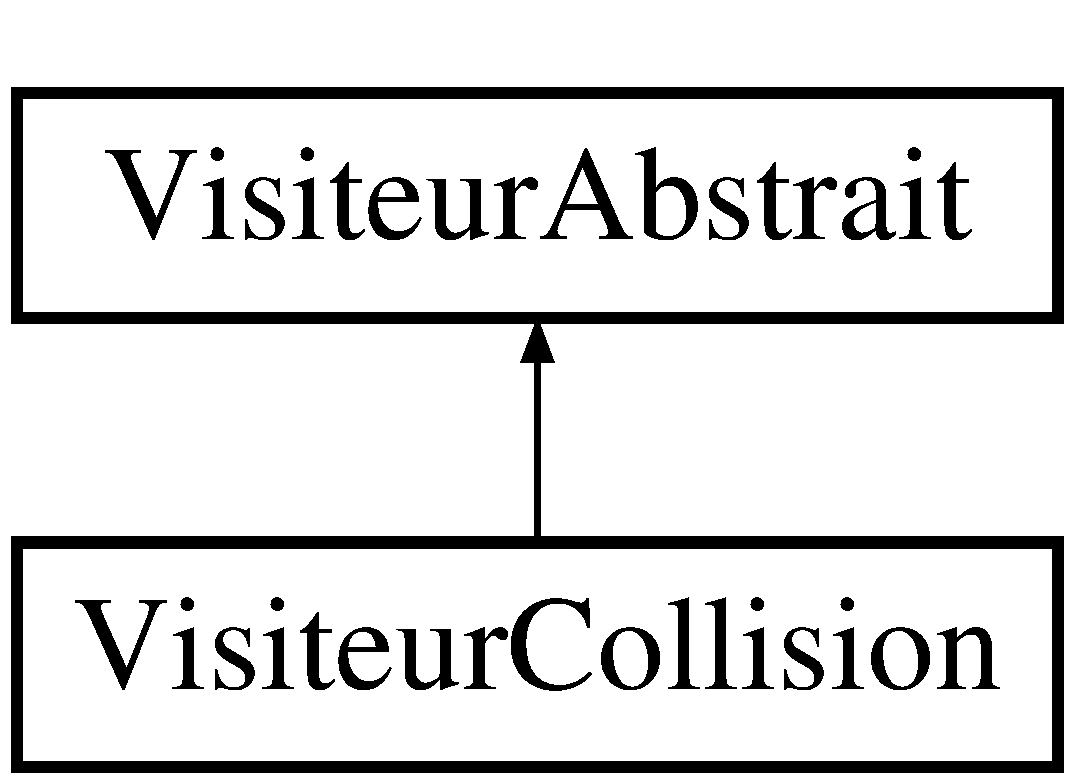
\includegraphics[height=2.000000cm]{class_visiteur_collision}
\end{center}
\end{figure}
\subsection*{Public Member Functions}
\begin{DoxyCompactItemize}
\item 
\hyperlink{class_visiteur_collision_adb7d5f275d9cf6cd9e9d74986058e700}{Visiteur\+Collision} ()
\item 
\hyperlink{class_visiteur_collision_a9383225a11bc84f3d5f3230b38df0d1f}{Visiteur\+Collision} (\hyperlink{class_noeud_rondelle}{Noeud\+Rondelle} $\ast$rondelle, double coef\+Rebon, std\+::vector$<$ \hyperlink{class_noeud_portail}{Noeud\+Portail} $\ast$$>$ portails, double acceleration)
\item 
\hyperlink{class_visiteur_collision_a92543e88d42df4f030c7e98737628d9a}{$\sim$\+Visiteur\+Collision} ()
\item 
\hypertarget{class_visiteur_collision_a289fb672e1cb408402cd4d5b0bc9fa7f}{}\label{class_visiteur_collision_a289fb672e1cb408402cd4d5b0bc9fa7f} 
void {\bfseries definir\+Position} (glm\+::dvec3)
\item 
void \hyperlink{class_visiteur_collision_a6bfba4fbee3a89120e5f78bdcccf535d}{definir\+Table} (\hyperlink{class_noeud_table}{Noeud\+Table} $\ast$)
\item 
virtual void \hyperlink{class_visiteur_collision_a60a7af24c85b42f39bdb9cf22b213f03}{visiter} (\hyperlink{class_noeud_composite}{Noeud\+Composite} $\ast$)
\item 
virtual void \hyperlink{class_visiteur_collision_ab5a50a3f4a1b1658eb0106a1f455fbaa}{visiter} (\hyperlink{class_noeud_maillet}{Noeud\+Maillet} $\ast$)
\item 
virtual void \hyperlink{class_visiteur_collision_a598b2bec9120bdc329721c94bb89b2b1}{visiter} (\hyperlink{class_noeud_maillet_virtuel}{Noeud\+Maillet\+Virtuel} $\ast$)
\item 
virtual void \hyperlink{class_visiteur_collision_a9a87666874976c2354ae6008c5d295ed}{visiter} (\hyperlink{class_noeud_muret}{Noeud\+Muret} $\ast$)
\item 
virtual void \hyperlink{class_visiteur_collision_a0dddecba0e89904757fca3d9081d678f}{visiter} (\hyperlink{class_noeud_portail}{Noeud\+Portail} $\ast$)
\item 
virtual void \hyperlink{class_visiteur_collision_ad679b2bdfe4bc0105ff638ddb5f447cc}{visiter} (\hyperlink{class_noeud_rondelle}{Noeud\+Rondelle} $\ast$)
\item 
virtual void \hyperlink{class_visiteur_collision_ab071b0f0b2d05d622c4698a652f19e77}{visiter} (\hyperlink{class_noeud_table}{Noeud\+Table} $\ast$)
\item 
virtual void \hyperlink{class_visiteur_collision_a9e56b43c1b38d5d4d08283d28b9dbcf2}{visiter} (\hyperlink{class_noeud_bonus_accelerateur}{Noeud\+Bonus\+Accelerateur} $\ast$)
\item 
void \hyperlink{class_visiteur_collision_a1918900085adcd2403fc8832ca04ede0}{reinitialiser\+Partie} ()
\item 
void \hyperlink{class_visiteur_collision_a9c727900f93230caf0bb10740a8ebd90}{quitter\+Portail} ()
\item 
\hypertarget{class_visiteur_collision_a689f17563d26e3953ef40baf7fb7f4e9}{}\label{class_visiteur_collision_a689f17563d26e3953ef40baf7fb7f4e9} 
int {\bfseries obtenir\+Buts\+Joueur1} ()
\item 
\hypertarget{class_visiteur_collision_ab602700bbcfdcb9aa49c41b56fabf784}{}\label{class_visiteur_collision_ab602700bbcfdcb9aa49c41b56fabf784} 
int {\bfseries obtenir\+Buts\+Joueur2} ()
\item 
void \hyperlink{class_visiteur_collision_a7e38363f989b24004ce4baba0c913957}{initialiser\+Scores} ()
\item 
int \hyperlink{class_visiteur_collision_aba0f1d8a18ad4cd19521159a73929aed}{get\+But\+JoueurG} ()
\item 
int \hyperlink{class_visiteur_collision_a13802f6045d791037e456906fa19a9ba}{get\+But\+JoueurD} ()
\item 
void \hyperlink{class_visiteur_collision_ab67aed0a6f062c2350eb6acc86f83508}{gerer\+Debogage} (string objet)
\item 
string \hyperlink{class_visiteur_collision_ae73a54932abf5972890c4b7c3ccf47ae}{afficher\+Temps} ()
\end{DoxyCompactItemize}
\subsection*{Additional Inherited Members}


\subsection{Constructor \& Destructor Documentation}
\hypertarget{class_visiteur_collision_adb7d5f275d9cf6cd9e9d74986058e700}{}\label{class_visiteur_collision_adb7d5f275d9cf6cd9e9d74986058e700} 
\index{Visiteur\+Collision@{Visiteur\+Collision}!Visiteur\+Collision@{Visiteur\+Collision}}
\index{Visiteur\+Collision@{Visiteur\+Collision}!Visiteur\+Collision@{Visiteur\+Collision}}
\subsubsection{\texorpdfstring{Visiteur\+Collision()}{VisiteurCollision()}\hspace{0.1cm}{\footnotesize\ttfamily [1/2]}}
{\footnotesize\ttfamily Visiteur\+Collision\+::\+Visiteur\+Collision (\begin{DoxyParamCaption}{ }\end{DoxyParamCaption})}

Constructeur par defaut, ne fait rien de special


\begin{DoxyParams}[1]{Parameters}
\mbox{\tt in}  & {\em Aucun} & \+: Rein defaut.\\
\hline
\end{DoxyParams}
\begin{DoxyReturn}{Returns}
Aucune. 
\end{DoxyReturn}
\hypertarget{class_visiteur_collision_a9383225a11bc84f3d5f3230b38df0d1f}{}\label{class_visiteur_collision_a9383225a11bc84f3d5f3230b38df0d1f} 
\index{Visiteur\+Collision@{Visiteur\+Collision}!Visiteur\+Collision@{Visiteur\+Collision}}
\index{Visiteur\+Collision@{Visiteur\+Collision}!Visiteur\+Collision@{Visiteur\+Collision}}
\subsubsection{\texorpdfstring{Visiteur\+Collision()}{VisiteurCollision()}\hspace{0.1cm}{\footnotesize\ttfamily [2/2]}}
{\footnotesize\ttfamily Visiteur\+Collision\+::\+Visiteur\+Collision (\begin{DoxyParamCaption}\item[{\hyperlink{class_noeud_rondelle}{Noeud\+Rondelle} $\ast$}]{rondelle,  }\item[{double}]{coef\+Rebon,  }\item[{std\+::vector$<$ \hyperlink{class_noeud_portail}{Noeud\+Portail} $\ast$$>$}]{portails,  }\item[{double}]{acceleration }\end{DoxyParamCaption})}

Constructeur par parametres


\begin{DoxyParams}[1]{Parameters}
\mbox{\tt in}  & {\em rondelle} & \+: la rondelle du jeux, coef\+Rebon \+: le coefficient de rebon de la table, portails \+: la liste de portails acceleration \+: l\textquotesingle{}acceleration de la table\\
\hline
\end{DoxyParams}
\begin{DoxyReturn}{Returns}
Aucune \+: constructeur. 
\end{DoxyReturn}
\hypertarget{class_visiteur_collision_a92543e88d42df4f030c7e98737628d9a}{}\label{class_visiteur_collision_a92543e88d42df4f030c7e98737628d9a} 
\index{Visiteur\+Collision@{Visiteur\+Collision}!````~Visiteur\+Collision@{$\sim$\+Visiteur\+Collision}}
\index{````~Visiteur\+Collision@{$\sim$\+Visiteur\+Collision}!Visiteur\+Collision@{Visiteur\+Collision}}
\subsubsection{\texorpdfstring{$\sim$\+Visiteur\+Collision()}{~VisiteurCollision()}}
{\footnotesize\ttfamily Visiteur\+Collision\+::$\sim$\+Visiteur\+Collision (\begin{DoxyParamCaption}{ }\end{DoxyParamCaption})}

Destructeur \+: desalloue la memoire


\begin{DoxyParams}[1]{Parameters}
\mbox{\tt in}  & {\em Aucun.} & \\
\hline
\end{DoxyParams}
\begin{DoxyReturn}{Returns}
Aucune. 
\end{DoxyReturn}


\subsection{Member Function Documentation}
\hypertarget{class_visiteur_collision_ae73a54932abf5972890c4b7c3ccf47ae}{}\label{class_visiteur_collision_ae73a54932abf5972890c4b7c3ccf47ae} 
\index{Visiteur\+Collision@{Visiteur\+Collision}!afficher\+Temps@{afficher\+Temps}}
\index{afficher\+Temps@{afficher\+Temps}!Visiteur\+Collision@{Visiteur\+Collision}}
\subsubsection{\texorpdfstring{afficher\+Temps()}{afficherTemps()}}
{\footnotesize\ttfamily string Visiteur\+Collision\+::afficher\+Temps (\begin{DoxyParamCaption}{ }\end{DoxyParamCaption})}

Cette fonction permet de calculer le temps.


\begin{DoxyParams}[1]{Parameters}
\mbox{\tt in}  & {\em Aucun.} & \\
\hline
\end{DoxyParams}
\begin{DoxyReturn}{Returns}
string \+: le temps dans le bon format. 
\end{DoxyReturn}
\hypertarget{class_visiteur_collision_a6bfba4fbee3a89120e5f78bdcccf535d}{}\label{class_visiteur_collision_a6bfba4fbee3a89120e5f78bdcccf535d} 
\index{Visiteur\+Collision@{Visiteur\+Collision}!definir\+Table@{definir\+Table}}
\index{definir\+Table@{definir\+Table}!Visiteur\+Collision@{Visiteur\+Collision}}
\subsubsection{\texorpdfstring{definir\+Table()}{definirTable()}}
{\footnotesize\ttfamily void Visiteur\+Collision\+::definir\+Table (\begin{DoxyParamCaption}\item[{\hyperlink{class_noeud_table}{Noeud\+Table} $\ast$}]{table }\end{DoxyParamCaption})}

Cette fonction permet de definir la table de jeu.


\begin{DoxyParams}[1]{Parameters}
\mbox{\tt in}  & {\em table} & \+: la table du jeu.\\
\hline
\end{DoxyParams}
\begin{DoxyReturn}{Returns}
Aucune. 
\end{DoxyReturn}
\hypertarget{class_visiteur_collision_ab67aed0a6f062c2350eb6acc86f83508}{}\label{class_visiteur_collision_ab67aed0a6f062c2350eb6acc86f83508} 
\index{Visiteur\+Collision@{Visiteur\+Collision}!gerer\+Debogage@{gerer\+Debogage}}
\index{gerer\+Debogage@{gerer\+Debogage}!Visiteur\+Collision@{Visiteur\+Collision}}
\subsubsection{\texorpdfstring{gerer\+Debogage()}{gererDebogage()}}
{\footnotesize\ttfamily void Visiteur\+Collision\+::gerer\+Debogage (\begin{DoxyParamCaption}\item[{string}]{objet }\end{DoxyParamCaption})}

Cette fonction affiche le debogage selon les booleans de l\textquotesingle{}utilisateur,


\begin{DoxyParams}[1]{Parameters}
\mbox{\tt in}  & {\em objet} & \+: l\textquotesingle{}objet avec qui la rondelle entre en collision.\\
\hline
\end{DoxyParams}
\begin{DoxyReturn}{Returns}
Aucune. 
\end{DoxyReturn}
\hypertarget{class_visiteur_collision_a13802f6045d791037e456906fa19a9ba}{}\label{class_visiteur_collision_a13802f6045d791037e456906fa19a9ba} 
\index{Visiteur\+Collision@{Visiteur\+Collision}!get\+But\+JoueurD@{get\+But\+JoueurD}}
\index{get\+But\+JoueurD@{get\+But\+JoueurD}!Visiteur\+Collision@{Visiteur\+Collision}}
\subsubsection{\texorpdfstring{get\+But\+Joueur\+D()}{getButJoueurD()}}
{\footnotesize\ttfamily int Visiteur\+Collision\+::get\+But\+JoueurD (\begin{DoxyParamCaption}{ }\end{DoxyParamCaption})}

Cette fonction retourne le nombre de but droite.


\begin{DoxyParams}[1]{Parameters}
\mbox{\tt in}  & {\em Aucun.} & \\
\hline
\end{DoxyParams}
\begin{DoxyReturn}{Returns}
le nombre de but du joueur droite. 
\end{DoxyReturn}
\hypertarget{class_visiteur_collision_aba0f1d8a18ad4cd19521159a73929aed}{}\label{class_visiteur_collision_aba0f1d8a18ad4cd19521159a73929aed} 
\index{Visiteur\+Collision@{Visiteur\+Collision}!get\+But\+JoueurG@{get\+But\+JoueurG}}
\index{get\+But\+JoueurG@{get\+But\+JoueurG}!Visiteur\+Collision@{Visiteur\+Collision}}
\subsubsection{\texorpdfstring{get\+But\+Joueur\+G()}{getButJoueurG()}}
{\footnotesize\ttfamily int Visiteur\+Collision\+::get\+But\+JoueurG (\begin{DoxyParamCaption}{ }\end{DoxyParamCaption})}

Cette fonction retourne le nombre de but gauche.


\begin{DoxyParams}[1]{Parameters}
\mbox{\tt in}  & {\em Aucun.} & \\
\hline
\end{DoxyParams}
\begin{DoxyReturn}{Returns}
le nombre de but du joueur gauche. 
\end{DoxyReturn}
\hypertarget{class_visiteur_collision_a7e38363f989b24004ce4baba0c913957}{}\label{class_visiteur_collision_a7e38363f989b24004ce4baba0c913957} 
\index{Visiteur\+Collision@{Visiteur\+Collision}!initialiser\+Scores@{initialiser\+Scores}}
\index{initialiser\+Scores@{initialiser\+Scores}!Visiteur\+Collision@{Visiteur\+Collision}}
\subsubsection{\texorpdfstring{initialiser\+Scores()}{initialiserScores()}}
{\footnotesize\ttfamily void Visiteur\+Collision\+::initialiser\+Scores (\begin{DoxyParamCaption}{ }\end{DoxyParamCaption})}

Cette fonction permet de reinitialiser le scores pour les deux joueurs.


\begin{DoxyParams}[1]{Parameters}
\mbox{\tt in}  & {\em Aucun.} & \\
\hline
\end{DoxyParams}
\begin{DoxyReturn}{Returns}
Aucune. 
\end{DoxyReturn}
\hypertarget{class_visiteur_collision_a9c727900f93230caf0bb10740a8ebd90}{}\label{class_visiteur_collision_a9c727900f93230caf0bb10740a8ebd90} 
\index{Visiteur\+Collision@{Visiteur\+Collision}!quitter\+Portail@{quitter\+Portail}}
\index{quitter\+Portail@{quitter\+Portail}!Visiteur\+Collision@{Visiteur\+Collision}}
\subsubsection{\texorpdfstring{quitter\+Portail()}{quitterPortail()}}
{\footnotesize\ttfamily void Visiteur\+Collision\+::quitter\+Portail (\begin{DoxyParamCaption}{ }\end{DoxyParamCaption})}

Cette fonction permet de pousser la rondelle a quitter le portail pour ne pas etre reabsorber.


\begin{DoxyParams}[1]{Parameters}
\mbox{\tt in}  & {\em Aucun.} & \\
\hline
\end{DoxyParams}
\begin{DoxyReturn}{Returns}
Aucune. 
\end{DoxyReturn}
\hypertarget{class_visiteur_collision_a1918900085adcd2403fc8832ca04ede0}{}\label{class_visiteur_collision_a1918900085adcd2403fc8832ca04ede0} 
\index{Visiteur\+Collision@{Visiteur\+Collision}!reinitialiser\+Partie@{reinitialiser\+Partie}}
\index{reinitialiser\+Partie@{reinitialiser\+Partie}!Visiteur\+Collision@{Visiteur\+Collision}}
\subsubsection{\texorpdfstring{reinitialiser\+Partie()}{reinitialiserPartie()}}
{\footnotesize\ttfamily void Visiteur\+Collision\+::reinitialiser\+Partie (\begin{DoxyParamCaption}{ }\end{DoxyParamCaption})}

Cette fonction permet de reinintialiser la la partie.


\begin{DoxyParams}[1]{Parameters}
\mbox{\tt in}  & {\em Aucun.} & \\
\hline
\end{DoxyParams}
\begin{DoxyReturn}{Returns}
Aucune. 
\end{DoxyReturn}
\hypertarget{class_visiteur_collision_a60a7af24c85b42f39bdb9cf22b213f03}{}\label{class_visiteur_collision_a60a7af24c85b42f39bdb9cf22b213f03} 
\index{Visiteur\+Collision@{Visiteur\+Collision}!visiter@{visiter}}
\index{visiter@{visiter}!Visiteur\+Collision@{Visiteur\+Collision}}
\subsubsection{\texorpdfstring{visiter()}{visiter()}\hspace{0.1cm}{\footnotesize\ttfamily [1/8]}}
{\footnotesize\ttfamily void Visiteur\+Collision\+::visiter (\begin{DoxyParamCaption}\item[{\hyperlink{class_noeud_composite}{Noeud\+Composite} $\ast$}]{noeud }\end{DoxyParamCaption})\hspace{0.3cm}{\ttfamily [virtual]}}

Cette fonction permet de visiter un noeud composite.


\begin{DoxyParams}[1]{Parameters}
\mbox{\tt in}  & {\em noeud} & \+: Le noeud a visiter.\\
\hline
\end{DoxyParams}
\begin{DoxyReturn}{Returns}
Aucune. 
\end{DoxyReturn}


Reimplemented from \hyperlink{class_visiteur_abstrait}{Visiteur\+Abstrait}.

\hypertarget{class_visiteur_collision_ab5a50a3f4a1b1658eb0106a1f455fbaa}{}\label{class_visiteur_collision_ab5a50a3f4a1b1658eb0106a1f455fbaa} 
\index{Visiteur\+Collision@{Visiteur\+Collision}!visiter@{visiter}}
\index{visiter@{visiter}!Visiteur\+Collision@{Visiteur\+Collision}}
\subsubsection{\texorpdfstring{visiter()}{visiter()}\hspace{0.1cm}{\footnotesize\ttfamily [2/8]}}
{\footnotesize\ttfamily void Visiteur\+Collision\+::visiter (\begin{DoxyParamCaption}\item[{\hyperlink{class_noeud_maillet}{Noeud\+Maillet} $\ast$}]{noeud }\end{DoxyParamCaption})\hspace{0.3cm}{\ttfamily [virtual]}}

Cette fonction permet de verifier si il y a eu collision entre le maillet et un autre objet.


\begin{DoxyParams}[1]{Parameters}
\mbox{\tt in}  & {\em noeud} & \+: Le noeud a visiter.\\
\hline
\end{DoxyParams}
\begin{DoxyReturn}{Returns}
Aucune. 
\end{DoxyReturn}


Reimplemented from \hyperlink{class_visiteur_abstrait}{Visiteur\+Abstrait}.

\hypertarget{class_visiteur_collision_a598b2bec9120bdc329721c94bb89b2b1}{}\label{class_visiteur_collision_a598b2bec9120bdc329721c94bb89b2b1} 
\index{Visiteur\+Collision@{Visiteur\+Collision}!visiter@{visiter}}
\index{visiter@{visiter}!Visiteur\+Collision@{Visiteur\+Collision}}
\subsubsection{\texorpdfstring{visiter()}{visiter()}\hspace{0.1cm}{\footnotesize\ttfamily [3/8]}}
{\footnotesize\ttfamily void Visiteur\+Collision\+::visiter (\begin{DoxyParamCaption}\item[{\hyperlink{class_noeud_maillet_virtuel}{Noeud\+Maillet\+Virtuel} $\ast$}]{noeud }\end{DoxyParamCaption})\hspace{0.3cm}{\ttfamily [virtual]}}

Cette fonction permet de verifier si il y a eu collision entre le maillet virtuelle et un autre objet.


\begin{DoxyParams}[1]{Parameters}
\mbox{\tt in}  & {\em noeud} & \+: Le noeud a visiter.\\
\hline
\end{DoxyParams}
\begin{DoxyReturn}{Returns}
Aucune. 
\end{DoxyReturn}


Reimplemented from \hyperlink{class_visiteur_abstrait}{Visiteur\+Abstrait}.

\hypertarget{class_visiteur_collision_a9a87666874976c2354ae6008c5d295ed}{}\label{class_visiteur_collision_a9a87666874976c2354ae6008c5d295ed} 
\index{Visiteur\+Collision@{Visiteur\+Collision}!visiter@{visiter}}
\index{visiter@{visiter}!Visiteur\+Collision@{Visiteur\+Collision}}
\subsubsection{\texorpdfstring{visiter()}{visiter()}\hspace{0.1cm}{\footnotesize\ttfamily [4/8]}}
{\footnotesize\ttfamily void Visiteur\+Collision\+::visiter (\begin{DoxyParamCaption}\item[{\hyperlink{class_noeud_muret}{Noeud\+Muret} $\ast$}]{noeud }\end{DoxyParamCaption})\hspace{0.3cm}{\ttfamily [virtual]}}

Cette fonction permet de verifier si il y a eu collision entre le muret et un autre objet.


\begin{DoxyParams}[1]{Parameters}
\mbox{\tt in}  & {\em noeud} & \+: Le noeud a visiter.\\
\hline
\end{DoxyParams}
\begin{DoxyReturn}{Returns}
Aucune. 
\end{DoxyReturn}


Reimplemented from \hyperlink{class_visiteur_abstrait}{Visiteur\+Abstrait}.

\hypertarget{class_visiteur_collision_a0dddecba0e89904757fca3d9081d678f}{}\label{class_visiteur_collision_a0dddecba0e89904757fca3d9081d678f} 
\index{Visiteur\+Collision@{Visiteur\+Collision}!visiter@{visiter}}
\index{visiter@{visiter}!Visiteur\+Collision@{Visiteur\+Collision}}
\subsubsection{\texorpdfstring{visiter()}{visiter()}\hspace{0.1cm}{\footnotesize\ttfamily [5/8]}}
{\footnotesize\ttfamily void Visiteur\+Collision\+::visiter (\begin{DoxyParamCaption}\item[{\hyperlink{class_noeud_portail}{Noeud\+Portail} $\ast$}]{noeud }\end{DoxyParamCaption})\hspace{0.3cm}{\ttfamily [virtual]}}

Cette fonction permet de verifier si il y a eu collision entre le portail et un autre objet.


\begin{DoxyParams}[1]{Parameters}
\mbox{\tt in}  & {\em noeud} & \+: Le noeud a visiter.\\
\hline
\end{DoxyParams}
\begin{DoxyReturn}{Returns}
Aucune. 
\end{DoxyReturn}


Reimplemented from \hyperlink{class_visiteur_abstrait}{Visiteur\+Abstrait}.

\hypertarget{class_visiteur_collision_ad679b2bdfe4bc0105ff638ddb5f447cc}{}\label{class_visiteur_collision_ad679b2bdfe4bc0105ff638ddb5f447cc} 
\index{Visiteur\+Collision@{Visiteur\+Collision}!visiter@{visiter}}
\index{visiter@{visiter}!Visiteur\+Collision@{Visiteur\+Collision}}
\subsubsection{\texorpdfstring{visiter()}{visiter()}\hspace{0.1cm}{\footnotesize\ttfamily [6/8]}}
{\footnotesize\ttfamily void Visiteur\+Collision\+::visiter (\begin{DoxyParamCaption}\item[{\hyperlink{class_noeud_rondelle}{Noeud\+Rondelle} $\ast$}]{noeud }\end{DoxyParamCaption})\hspace{0.3cm}{\ttfamily [virtual]}}

Cette fonction permet de verifier si il y a eu collision entre la rondelle et un autre objet.


\begin{DoxyParams}[1]{Parameters}
\mbox{\tt in}  & {\em noeud} & \+: Le noeud a visiter.\\
\hline
\end{DoxyParams}
\begin{DoxyReturn}{Returns}
Aucune. 
\end{DoxyReturn}


Reimplemented from \hyperlink{class_visiteur_abstrait}{Visiteur\+Abstrait}.

\hypertarget{class_visiteur_collision_ab071b0f0b2d05d622c4698a652f19e77}{}\label{class_visiteur_collision_ab071b0f0b2d05d622c4698a652f19e77} 
\index{Visiteur\+Collision@{Visiteur\+Collision}!visiter@{visiter}}
\index{visiter@{visiter}!Visiteur\+Collision@{Visiteur\+Collision}}
\subsubsection{\texorpdfstring{visiter()}{visiter()}\hspace{0.1cm}{\footnotesize\ttfamily [7/8]}}
{\footnotesize\ttfamily void Visiteur\+Collision\+::visiter (\begin{DoxyParamCaption}\item[{\hyperlink{class_noeud_table}{Noeud\+Table} $\ast$}]{noeud }\end{DoxyParamCaption})\hspace{0.3cm}{\ttfamily [virtual]}}

Cette fonction permet de verifier si il y a eu collision entre la table et un autre objet, elle permet aussi de visiter ses enfants.


\begin{DoxyParams}[1]{Parameters}
\mbox{\tt in}  & {\em noeud} & \+: Le noeud a visiter.\\
\hline
\end{DoxyParams}
\begin{DoxyReturn}{Returns}
Aucune. 
\end{DoxyReturn}


Reimplemented from \hyperlink{class_visiteur_abstrait}{Visiteur\+Abstrait}.

\hypertarget{class_visiteur_collision_a9e56b43c1b38d5d4d08283d28b9dbcf2}{}\label{class_visiteur_collision_a9e56b43c1b38d5d4d08283d28b9dbcf2} 
\index{Visiteur\+Collision@{Visiteur\+Collision}!visiter@{visiter}}
\index{visiter@{visiter}!Visiteur\+Collision@{Visiteur\+Collision}}
\subsubsection{\texorpdfstring{visiter()}{visiter()}\hspace{0.1cm}{\footnotesize\ttfamily [8/8]}}
{\footnotesize\ttfamily void Visiteur\+Collision\+::visiter (\begin{DoxyParamCaption}\item[{\hyperlink{class_noeud_bonus_accelerateur}{Noeud\+Bonus\+Accelerateur} $\ast$}]{noeud }\end{DoxyParamCaption})\hspace{0.3cm}{\ttfamily [virtual]}}

Cette fonction permet de verifier si il y a eu collision entre le bonus d\textquotesingle{}acceleration et un autre objet.


\begin{DoxyParams}[1]{Parameters}
\mbox{\tt in}  & {\em noeud} & \+: Le noeud a visiter.\\
\hline
\end{DoxyParams}
\begin{DoxyReturn}{Returns}
Aucune. 
\end{DoxyReturn}


Reimplemented from \hyperlink{class_visiteur_abstrait}{Visiteur\+Abstrait}.



The documentation for this class was generated from the following files\+:\begin{DoxyCompactItemize}
\item 
C\+:/\+Users/\+Steven/\+Documents/\+Poly/\+I\+N\+F2990/inf2990-\/06/\+Cadriciel\+\_\+2016-\/3\+\_\+\+Etudiants/\+Cadriciel/\+Sources/\+D\+L\+L/Visiteur\+Collision.\+h\item 
C\+:/\+Users/\+Steven/\+Documents/\+Poly/\+I\+N\+F2990/inf2990-\/06/\+Cadriciel\+\_\+2016-\/3\+\_\+\+Etudiants/\+Cadriciel/\+Sources/\+D\+L\+L/Visiteur\+Collision.\+cpp\end{DoxyCompactItemize}

\hypertarget{class_visiteur_deplacement}{}\section{Visiteur\+Deplacement Class Reference}
\label{class_visiteur_deplacement}\index{Visiteur\+Deplacement@{Visiteur\+Deplacement}}
Inheritance diagram for Visiteur\+Deplacement\+:\begin{figure}[H]
\begin{center}
\leavevmode
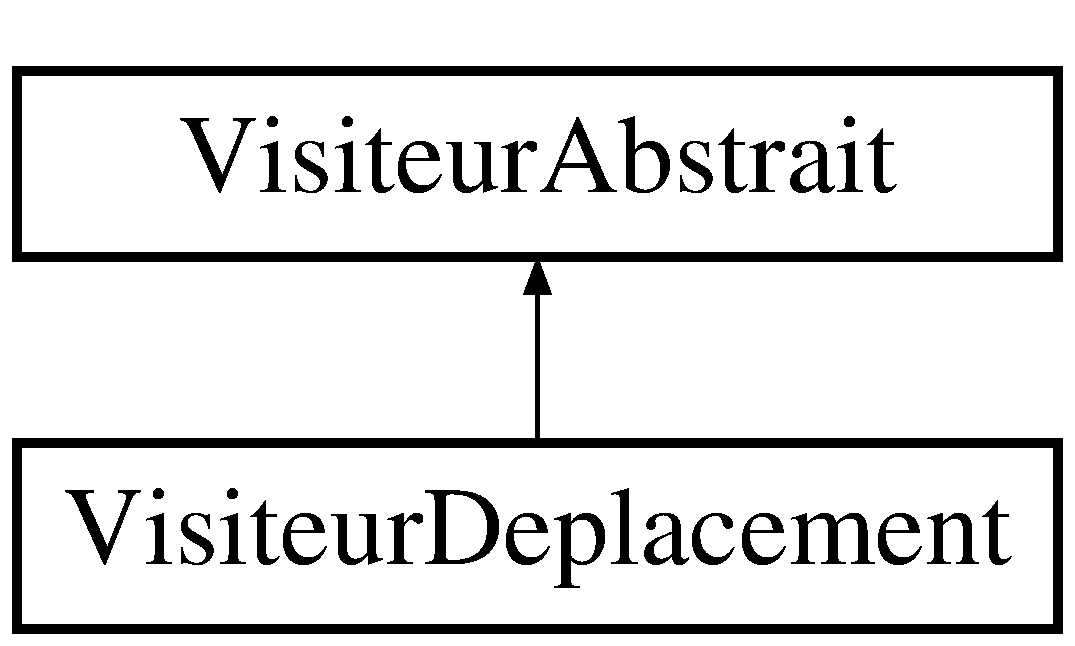
\includegraphics[height=2.000000cm]{class_visiteur_deplacement}
\end{center}
\end{figure}
\subsection*{Public Member Functions}
\begin{DoxyCompactItemize}
\item 
\hyperlink{group__inf2990_ga96164e1d4e72549c09424358e8f01e78}{Visiteur\+Deplacement} ()
\begin{DoxyCompactList}\small\item\em constructor \end{DoxyCompactList}\item 
\hyperlink{group__inf2990_ga0f03274d6afe77a7a57f3b7f20417ec8}{$\sim$\+Visiteur\+Deplacement} ()
\begin{DoxyCompactList}\small\item\em destructeur \end{DoxyCompactList}\item 
void \hyperlink{group__inf2990_ga882cdd41499aab95ccc1eecbafebbb09}{modifier\+Position} (glm\+::dvec3 \hyperlink{structposition}{position})
\begin{DoxyCompactList}\small\item\em modificateurs \end{DoxyCompactList}\item 
float \hyperlink{group__inf2990_ga1be5d6505e3355287b55d5fbe448e600}{obtenirX} ()
\begin{DoxyCompactList}\small\item\em recuperateurs \end{DoxyCompactList}\item 
float {\bfseries obtenirY} ()
\item 
float {\bfseries obtenirZ} ()
\item 
virtual void \hyperlink{group__inf2990_ga2d81940a4fd36b6c5ea00ef022191dc8}{visiter} (\hyperlink{class_noeud_composite}{Noeud\+Composite} $\ast$noeud)
\begin{DoxyCompactList}\small\item\em visites des differents noeuds \end{DoxyCompactList}\item 
virtual void \hyperlink{group__inf2990_gac3e9945e0d76cd90f7f7722fccd74298}{visiter} (\hyperlink{class_noeud_maillet}{Noeud\+Maillet} $\ast$noeud)
\item 
virtual void \hyperlink{group__inf2990_ga2c4d7672f376bd635318a0e987e696ed}{visiter} (\hyperlink{class_noeud_muret}{Noeud\+Muret} $\ast$noeud)
\item 
virtual void \hyperlink{group__inf2990_ga27370e2a2e188d7d209e20e4e8228f42}{visiter} (\hyperlink{class_noeud_portail}{Noeud\+Portail} $\ast$noeud)
\item 
virtual void \hyperlink{group__inf2990_ga9b1dde6c8d6e7dab86ffa64925b62edd}{visiter} (\hyperlink{class_noeud_rondelle}{Noeud\+Rondelle} $\ast$noeud)
\item 
virtual void \hyperlink{group__inf2990_ga9599fc0f1de752c95febe9315eefc808}{visiter} (\hyperlink{class_noeud_table}{Noeud\+Table} $\ast$noeud)
\item 
virtual void \hyperlink{group__inf2990_gaa214ddf720db2c3969d3bde0e5e1ce3a}{visiter} (\hyperlink{class_noeud_bonus_accelerateur}{Noeud\+Bonus\+Accelerateur} $\ast$noeud)
\end{DoxyCompactItemize}
\subsection*{Additional Inherited Members}


The documentation for this class was generated from the following files\+:\begin{DoxyCompactItemize}
\item 
Sources/\+D\+L\+L/\hyperlink{_visiteur_deplacement_8h}{Visiteur\+Deplacement.\+h}\item 
Sources/\+D\+L\+L/\hyperlink{_visiteur_deplacement_8cpp}{Visiteur\+Deplacement.\+cpp}\item 
Sources/\+D\+L\+L/\hyperlink{_visiteur_echelle_8cpp}{Visiteur\+Echelle.\+cpp}\end{DoxyCompactItemize}

\hypertarget{class_visiteur_deplacement_test}{}\section{Visiteur\+Deplacement\+Test Class Reference}
\label{class_visiteur_deplacement_test}\index{Visiteur\+Deplacement\+Test@{Visiteur\+Deplacement\+Test}}
Inheritance diagram for Visiteur\+Deplacement\+Test\+:\begin{figure}[H]
\begin{center}
\leavevmode
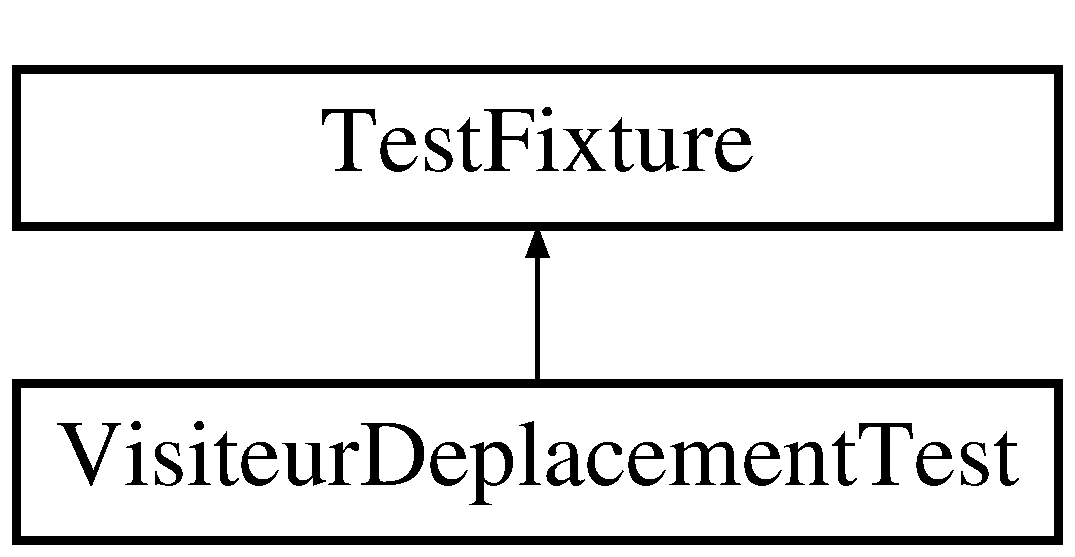
\includegraphics[height=2.000000cm]{class_visiteur_deplacement_test}
\end{center}
\end{figure}
\subsection*{Public Member Functions}
\begin{DoxyCompactItemize}
\item 
void \hyperlink{group__inf2990_gaa1a354e68a9671b2816d598f2bc8a515}{set\+Up} ()
\begin{DoxyCompactList}\small\item\em Traitement � effectuer pour initialiser cette suite de tests. \end{DoxyCompactList}\item 
void \hyperlink{group__inf2990_ga1dff6fee4b3decb9a3a87367316b4410}{tear\+Down} ()
\begin{DoxyCompactList}\small\item\em Traitement � effectuer pour \textquotesingle{}finaliser\textquotesingle{} cette suite de tests. \end{DoxyCompactList}\item 
void \hyperlink{group__inf2990_ga55cbfcefbc9f140ad2787387ac610c3a}{test\+Deplacement} ()
\begin{DoxyCompactList}\small\item\em Cas de test\+: �criture/lecture de la position relative. \end{DoxyCompactList}\end{DoxyCompactItemize}


The documentation for this class was generated from the following files\+:\begin{DoxyCompactItemize}
\item 
C\+:/\+Users/\+Steven/\+Documents/\+Poly/\+I\+N\+F2990/inf2990-\/06/\+Cadriciel\+\_\+2016-\/3\+\_\+\+Etudiants/\+Cadriciel/\+Sources/\+D\+L\+L/\hyperlink{_visiteur_deplacement_test_8h}{Visiteur\+Deplacement\+Test.\+h}\item 
C\+:/\+Users/\+Steven/\+Documents/\+Poly/\+I\+N\+F2990/inf2990-\/06/\+Cadriciel\+\_\+2016-\/3\+\_\+\+Etudiants/\+Cadriciel/\+Sources/\+D\+L\+L/\hyperlink{_visiteur_deplacement_test_8cpp}{Visiteur\+Deplacement\+Test.\+cpp}\end{DoxyCompactItemize}

\hypertarget{class_visiteur_duplication}{}\section{Visiteur\+Duplication Class Reference}
\label{class_visiteur_duplication}\index{Visiteur\+Duplication@{Visiteur\+Duplication}}
Inheritance diagram for Visiteur\+Duplication\+:\begin{figure}[H]
\begin{center}
\leavevmode
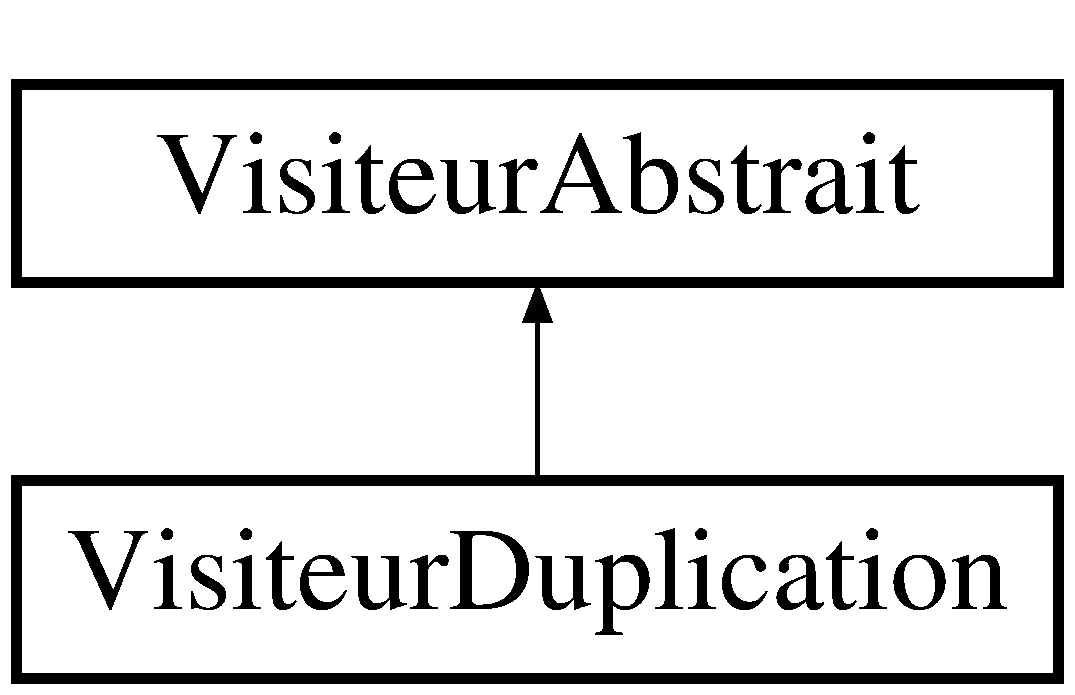
\includegraphics[height=2.000000cm]{class_visiteur_duplication}
\end{center}
\end{figure}
\subsection*{Public Member Functions}
\begin{DoxyCompactItemize}
\item 
\hyperlink{group__inf2990_gab7f16d7325839d400df6da191430fbd8}{Visiteur\+Duplication} (\hyperlink{class_arbre_rendu_i_n_f2990}{Arbre\+Rendu\+I\+N\+F2990} $\ast$)
\item 
\hyperlink{group__inf2990_gab48c0bd69fe4738d85ec48bfe1ae51ea}{$\sim$\+Visiteur\+Duplication} ()
\item 
void \hyperlink{group__inf2990_ga1482d7144bc781ddbef06292573872a8}{definir\+Position} (glm\+::dvec3)
\item 
void \hyperlink{group__inf2990_ga44443631965b05df20db383d723765e2}{deplacer\+Etampe} ()
\item 
virtual void \hyperlink{group__inf2990_gaa66f13da730ff20959fd4c7b24c2c6ea}{visiter} (\hyperlink{class_noeud_composite}{Noeud\+Composite} $\ast$)
\item 
virtual void \hyperlink{group__inf2990_ga0300496a83fea5642c06b86fce6cd17e}{visiter} (\hyperlink{class_noeud_maillet}{Noeud\+Maillet} $\ast$)
\item 
virtual void \hyperlink{group__inf2990_ga03689e8ff1b47c750834eb2d593b8fcf}{visiter} (\hyperlink{class_noeud_muret}{Noeud\+Muret} $\ast$)
\item 
virtual void {\bfseries visiter} (\hyperlink{class_noeud_portail}{Noeud\+Portail} $\ast$)
\item 
virtual void {\bfseries visiter} (\hyperlink{class_noeud_rondelle}{Noeud\+Rondelle} $\ast$)
\item 
virtual void \hyperlink{group__inf2990_gab0e86c310bdfeeddf6787dc8a25030ef}{visiter} (\hyperlink{class_noeud_table}{Noeud\+Table} $\ast$)
\item 
virtual void {\bfseries visiter} (\hyperlink{class_noeud_bonus_accelerateur}{Noeud\+Bonus\+Accelerateur} $\ast$)
\end{DoxyCompactItemize}
\subsection*{Additional Inherited Members}


The documentation for this class was generated from the following files\+:\begin{DoxyCompactItemize}
\item 
Sources/\+D\+L\+L/Visiteur\+Duplication.\+h\item 
Sources/\+D\+L\+L/\hyperlink{_visiteur_duplication_8cpp}{Visiteur\+Duplication.\+cpp}\end{DoxyCompactItemize}

\hypertarget{class_visiteur_echelle}{}\section{Visiteur\+Echelle Class Reference}
\label{class_visiteur_echelle}\index{Visiteur\+Echelle@{Visiteur\+Echelle}}
Inheritance diagram for Visiteur\+Echelle\+:\begin{figure}[H]
\begin{center}
\leavevmode
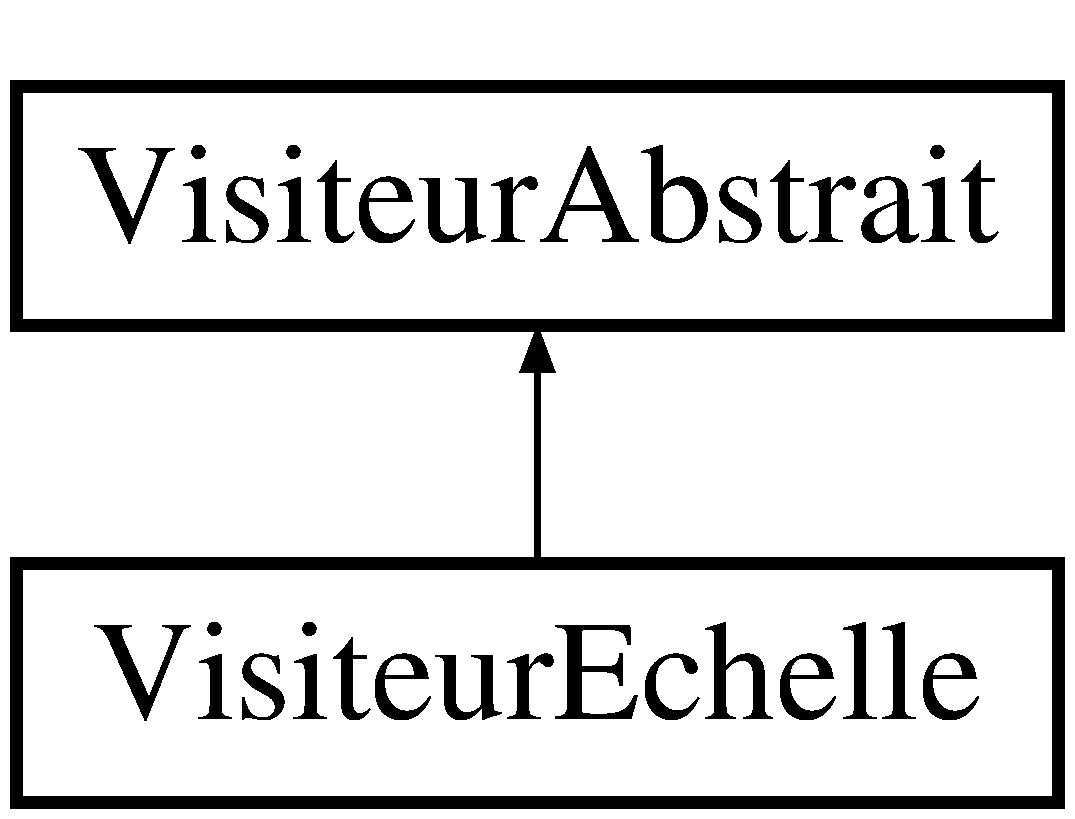
\includegraphics[height=2.000000cm]{class_visiteur_echelle}
\end{center}
\end{figure}
\subsection*{Public Member Functions}
\begin{DoxyCompactItemize}
\item 
\hyperlink{group__inf2990_gaddf0654645ae3598073fb8ec209c62ff}{Visiteur\+Echelle} (double facteur=1.\+0)
\item 
\hyperlink{group__inf2990_gaefd75264dd515e96588720d78698cb43}{$\sim$\+Visiteur\+Echelle} ()
\item 
void \hyperlink{group__inf2990_ga499407dd8991f64b30fc120017ab4090}{modifier\+Facteur} (double facteur)
\item 
double \hyperlink{group__inf2990_gae9b1f432611d822d61c595eaff646009}{obtenir\+Facteur} ()
\item 
virtual void {\bfseries visiter} (\hyperlink{class_noeud_composite}{Noeud\+Composite} $\ast$)
\item 
virtual void \hyperlink{group__inf2990_ga5cde1fb2bc7754fb7f9ce9943deafbc2}{visiter} (\hyperlink{class_noeud_maillet}{Noeud\+Maillet} $\ast$)
\item 
virtual void \hyperlink{group__inf2990_ga66c3727bc8cb483ce19c66a933a1e171}{visiter} (\hyperlink{class_noeud_muret}{Noeud\+Muret} $\ast$)
\item 
virtual void \hyperlink{group__inf2990_gab0abc0f847cb7abda9f002229e88829f}{visiter} (\hyperlink{class_noeud_portail}{Noeud\+Portail} $\ast$)
\item 
virtual void \hyperlink{group__inf2990_gadb69bccd2cfe72d73f860e3a4eabee7d}{visiter} (\hyperlink{class_noeud_rondelle}{Noeud\+Rondelle} $\ast$)
\item 
virtual void \hyperlink{group__inf2990_ga727e8d9127b63b580d4d3297a79332f1}{visiter} (\hyperlink{class_noeud_table}{Noeud\+Table} $\ast$)
\end{DoxyCompactItemize}
\subsection*{Additional Inherited Members}


The documentation for this class was generated from the following files\+:\begin{DoxyCompactItemize}
\item 
Sources/\+D\+L\+L/Visiteur\+Echelle.\+h\item 
Sources/\+D\+L\+L/\hyperlink{_visiteur_echelle_8cpp}{Visiteur\+Echelle.\+cpp}\end{DoxyCompactItemize}

\hypertarget{class_visiteur_ecriture_x_m_l}{}\section{Visiteur\+Ecriture\+X\+ML Class Reference}
\label{class_visiteur_ecriture_x_m_l}\index{Visiteur\+Ecriture\+X\+ML@{Visiteur\+Ecriture\+X\+ML}}
Inheritance diagram for Visiteur\+Ecriture\+X\+ML\+:\begin{figure}[H]
\begin{center}
\leavevmode
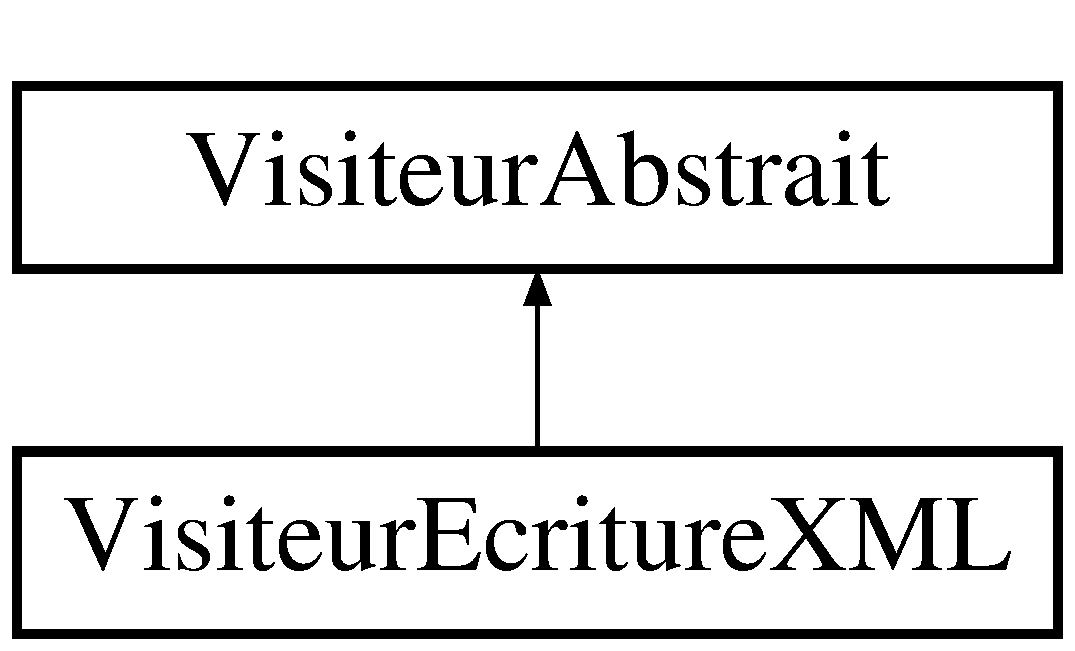
\includegraphics[height=2.000000cm]{class_visiteur_ecriture_x_m_l}
\end{center}
\end{figure}
\subsection*{Public Member Functions}
\begin{DoxyCompactItemize}
\item 
\hyperlink{group__inf2990_ga603ad88ebfda35e755544b4914b074ca}{Visiteur\+Ecriture\+X\+ML} (tinyxml2\+::\+X\+M\+L\+Element $\ast$racine)
\begin{DoxyCompactList}\small\item\em constructor \end{DoxyCompactList}\item 
\hyperlink{group__inf2990_gadf7aaa7cf24b9db027fae1d7311e88f4}{$\sim$\+Visiteur\+Ecriture\+X\+ML} ()
\begin{DoxyCompactList}\small\item\em destructeur \end{DoxyCompactList}\item 
virtual void \hyperlink{group__inf2990_ga7f22cab13593b84b8ce9a12f5a1ee20d}{visiter} (\hyperlink{class_noeud_composite}{Noeud\+Composite} $\ast$noeud)
\begin{DoxyCompactList}\small\item\em visites des differents noeuds \end{DoxyCompactList}\item 
virtual void \hyperlink{group__inf2990_ga03542b458767240b58f461c3d3b2a024}{visiter} (\hyperlink{class_noeud_maillet}{Noeud\+Maillet} $\ast$noeud)
\item 
virtual void \hyperlink{group__inf2990_gaea398607589ad92ffbf72fceebf3058c}{visiter} (\hyperlink{class_noeud_muret}{Noeud\+Muret} $\ast$noeud)
\item 
virtual void \hyperlink{group__inf2990_ga33c4411d6c8a5a4aa5de730e282d1b33}{visiter} (\hyperlink{class_noeud_portail}{Noeud\+Portail} $\ast$noeud)
\item 
virtual void \hyperlink{group__inf2990_ga56944b1a695729e789a8bdec7bec424f}{visiter} (\hyperlink{class_noeud_rondelle}{Noeud\+Rondelle} $\ast$noeud)
\item 
virtual void \hyperlink{group__inf2990_gaeb2a78298e8c18d34d1f9eee1920b419}{visiter} (\hyperlink{class_noeud_table}{Noeud\+Table} $\ast$noeud)
\item 
virtual void \hyperlink{group__inf2990_gaf4c4c56ab75e918739abbc00b274c938}{visiter} (\hyperlink{class_noeud_bonus_accelerateur}{Noeud\+Bonus\+Accelerateur} $\ast$noeud)
\end{DoxyCompactItemize}
\subsection*{Public Attributes}
\begin{DoxyCompactItemize}
\item 
tinyxml2\+::\+X\+M\+L\+Element $\ast$ \hyperlink{group__inf2990_ga40b822db4ca8fb0b9d9fa2801562ad03}{racine\+\_\+}
\begin{DoxyCompactList}\small\item\em Racine. \end{DoxyCompactList}\end{DoxyCompactItemize}
\subsection*{Additional Inherited Members}


The documentation for this class was generated from the following files\+:\begin{DoxyCompactItemize}
\item 
Sources/\+D\+L\+L/\hyperlink{_visiteur_ecriture_x_m_l_8h}{Visiteur\+Ecriture\+X\+M\+L.\+h}\item 
Sources/\+D\+L\+L/\hyperlink{_visiteur_ecriture_x_m_l_8cpp}{Visiteur\+Ecriture\+X\+M\+L.\+cpp}\end{DoxyCompactItemize}

\hypertarget{class_visiteur_rotation}{}\section{Visiteur\+Rotation Class Reference}
\label{class_visiteur_rotation}\index{Visiteur\+Rotation@{Visiteur\+Rotation}}
Inheritance diagram for Visiteur\+Rotation\+:\begin{figure}[H]
\begin{center}
\leavevmode
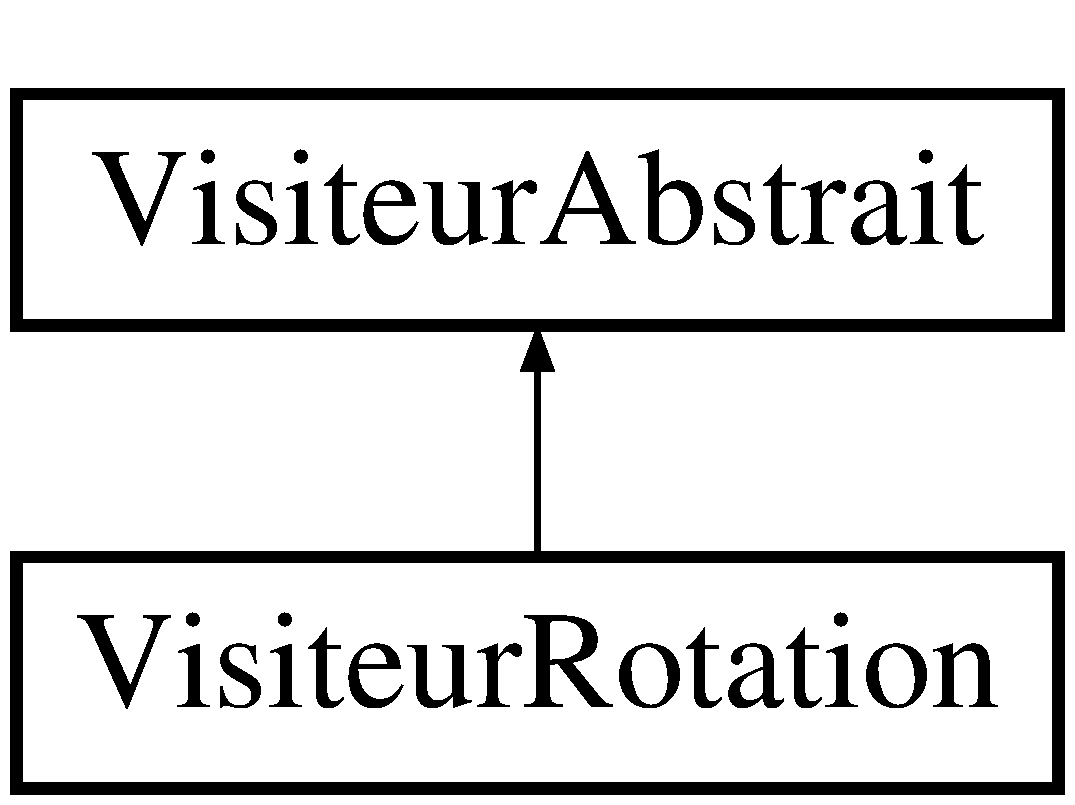
\includegraphics[height=2.000000cm]{class_visiteur_rotation}
\end{center}
\end{figure}
\subsection*{Public Member Functions}
\begin{DoxyCompactItemize}
\item 
\hyperlink{group__inf2990_ga18c6ce771b0372f1ae0972bdfbb961db}{Visiteur\+Rotation} (float centreX, float centreY, float varY)
\item 
float \hyperlink{group__inf2990_gab2365dc2295d046daf14cb3a52a61b41}{obtenir\+CentreX} ()
\item 
float \hyperlink{group__inf2990_ga04725f30de6cb19bc3a454ca5277afb9}{obtenir\+CentreY} ()
\item 
float \hyperlink{group__inf2990_ga8a151654f1636823250dc281de697ceb}{obtenir\+VarY} ()
\item 
void \hyperlink{group__inf2990_gad972a3de4ea8cffa5e81f99be35702dd}{modifier\+Centre} (float X, float Y)
\item 
void {\bfseries modifier\+VarY} (float varY)
\item 
virtual void \hyperlink{group__inf2990_ga8b2f030257b78e64844d3d6526fad507}{visiter} (\hyperlink{class_noeud_composite}{Noeud\+Composite} $\ast$noeud)
\item 
virtual void \hyperlink{group__inf2990_gaae32e22552eb3261ac6d5eaf8812acd8}{visiter} (\hyperlink{class_noeud_maillet}{Noeud\+Maillet} $\ast$noeud)
\item 
virtual void \hyperlink{group__inf2990_gaeb02b7e545154c48ea047ba90aa547ee}{visiter} (\hyperlink{class_noeud_muret}{Noeud\+Muret} $\ast$noeud)
\item 
virtual void \hyperlink{group__inf2990_gaed9327add2f03b3874c84629b7f8d1dd}{visiter} (\hyperlink{class_noeud_portail}{Noeud\+Portail} $\ast$noeud)
\item 
virtual void \hyperlink{group__inf2990_gae090f20239c6bf70aa11b858aa79a4fa}{visiter} (\hyperlink{class_noeud_rondelle}{Noeud\+Rondelle} $\ast$noeud)
\item 
virtual void {\bfseries visiter} (\hyperlink{class_noeud_table}{Noeud\+Table} $\ast$noeud)
\item 
virtual void \hyperlink{group__inf2990_ga30b9ecc99d9bb3f86963f795ee76a1c4}{visiter} (\hyperlink{class_noeud_bonus_accelerateur}{Noeud\+Bonus\+Accelerateur} $\ast$noeud)
\end{DoxyCompactItemize}
\subsection*{Additional Inherited Members}


The documentation for this class was generated from the following files\+:\begin{DoxyCompactItemize}
\item 
C\+:/\+Users/\+Steven/\+Documents/\+Poly/\+I\+N\+F2990/inf2990-\/06/\+Cadriciel\+\_\+2016-\/3\+\_\+\+Etudiants/\+Cadriciel/\+Sources/\+D\+L\+L/Visiteur\+Rotation.\+h\item 
C\+:/\+Users/\+Steven/\+Documents/\+Poly/\+I\+N\+F2990/inf2990-\/06/\+Cadriciel\+\_\+2016-\/3\+\_\+\+Etudiants/\+Cadriciel/\+Sources/\+D\+L\+L/\hyperlink{_visiteur_rotation_8cpp}{Visiteur\+Rotation.\+cpp}\end{DoxyCompactItemize}

\hypertarget{class_visiteur_selection}{}\section{Visiteur\+Selection Class Reference}
\label{class_visiteur_selection}\index{Visiteur\+Selection@{Visiteur\+Selection}}
Inheritance diagram for Visiteur\+Selection\+:\begin{figure}[H]
\begin{center}
\leavevmode
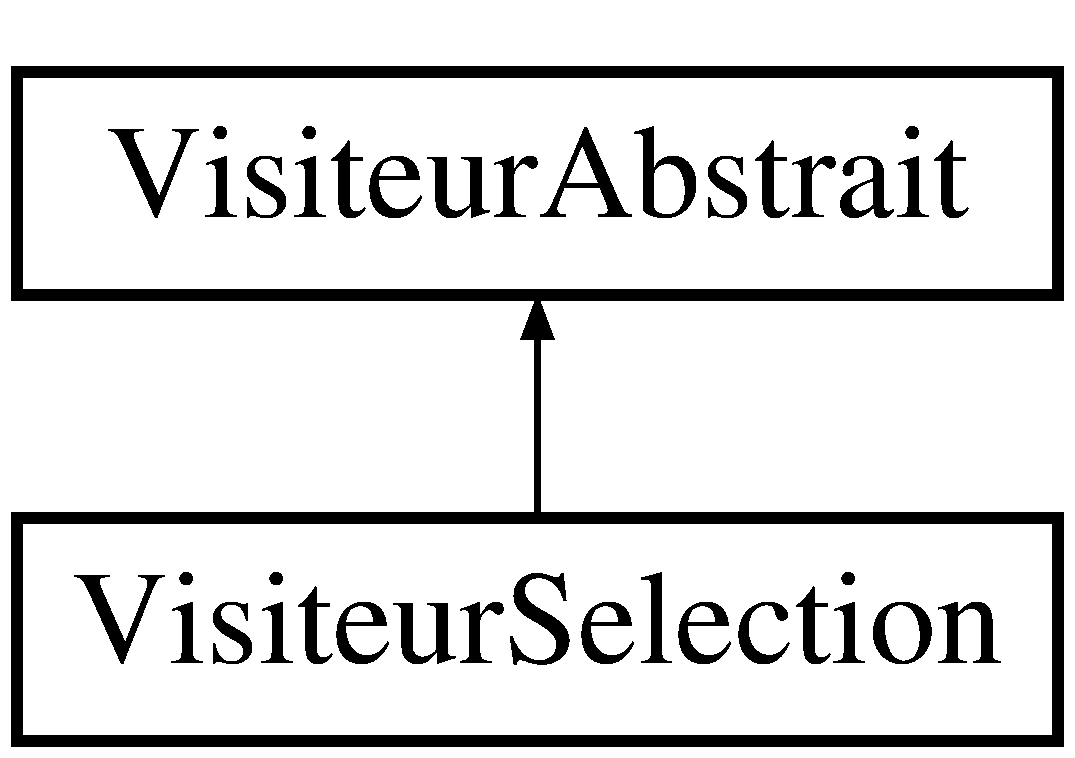
\includegraphics[height=2.000000cm]{class_visiteur_selection}
\end{center}
\end{figure}
\subsection*{Public Member Functions}
\begin{DoxyCompactItemize}
\item 
\hypertarget{class_visiteur_selection_abfa92ff155e59d64ab79d2f6530715ff}{}\label{class_visiteur_selection_abfa92ff155e59d64ab79d2f6530715ff} 
\hyperlink{class_visiteur_selection_abfa92ff155e59d64ab79d2f6530715ff}{Visiteur\+Selection} (glm\+::dvec3 \&point, bool selection\+Unique, G\+Lubyte couleur\+Pixel\mbox{[}$\,$\mbox{]}, const bool \&initialiser\+Visite)
\begin{DoxyCompactList}\small\item\em Constucteur. \end{DoxyCompactList}\item 
virtual void \hyperlink{group__inf2990_gaf6d77b8c875bda7f01434cf4e834599c}{visiter} (\hyperlink{class_noeud_composite}{Noeud\+Composite} $\ast$)
\item 
virtual void \hyperlink{group__inf2990_ga5576bd68b32506507c788027a8804cff}{visiter} (\hyperlink{class_noeud_portail}{Noeud\+Portail} $\ast$noeud)
\begin{DoxyCompactList}\small\item\em Algorithme de visite pour \hyperlink{class_noeud_portail}{Noeud\+Portail}. \end{DoxyCompactList}\item 
virtual void \hyperlink{group__inf2990_ga91d77668ef5dad7e42a9d9876d7464da}{visiter} (\hyperlink{class_noeud_muret}{Noeud\+Muret} $\ast$noeud)
\begin{DoxyCompactList}\small\item\em Algorithme de visite pour \hyperlink{class_noeud_muret}{Noeud\+Muret}. \end{DoxyCompactList}\item 
virtual void \hyperlink{group__inf2990_ga6b291b464d019af9696d2916ae58dc23}{visiter} (\hyperlink{class_noeud_maillet}{Noeud\+Maillet} $\ast$noeud)
\begin{DoxyCompactList}\small\item\em Algorithme de visite pour \hyperlink{class_noeud_table}{Noeud\+Table}. \end{DoxyCompactList}\item 
virtual void \hyperlink{group__inf2990_gaa00c8b4c2a981faf4b6bd5ecdafc3427}{visiter} (\hyperlink{class_noeud_bonus_accelerateur}{Noeud\+Bonus\+Accelerateur} $\ast$noeud)
\item 
virtual void \hyperlink{group__inf2990_ga81f3ec46afbfe7fdbc5a3406991e00b7}{visiter} (\hyperlink{class_noeud_rondelle}{Noeud\+Rondelle} $\ast$noeud)
\item 
\hypertarget{class_visiteur_selection_aa2882688ed42325b7ecf6b17be4fcc72}{}\label{class_visiteur_selection_aa2882688ed42325b7ecf6b17be4fcc72} 
bool \hyperlink{class_visiteur_selection_aa2882688ed42325b7ecf6b17be4fcc72}{obtenirselection\+Existe} ()
\begin{DoxyCompactList}\small\item\em Methode permettant le retour de la selectionexiste. \end{DoxyCompactList}\end{DoxyCompactItemize}
\subsection*{Additional Inherited Members}


The documentation for this class was generated from the following files\+:\begin{DoxyCompactItemize}
\item 
Sources/\+D\+L\+L/Visiteur\+Selection.\+h\item 
Sources/\+D\+L\+L/Visiteur\+Selection.\+cpp\end{DoxyCompactItemize}

\hypertarget{class_visiteur_select_objet}{}\section{Visiteur\+Select\+Objet Class Reference}
\label{class_visiteur_select_objet}\index{Visiteur\+Select\+Objet@{Visiteur\+Select\+Objet}}


Classe qui impl�mentante le visiteur concr�t permettant de parcourir l\textquotesingle{}arbre de rendu et de visiter chaque noeud afin de permettre la selection par clic.  




{\ttfamily \#include $<$Visiteur\+Selection.\+h$>$}



\subsection{Detailed Description}
Classe qui impl�mentante le visiteur concr�t permettant de parcourir l\textquotesingle{}arbre de rendu et de visiter chaque noeud afin de permettre la selection par clic. 

Les visiteurs concr�ts pourront faire diff�rents tra�tements en fonction du type de noeud visit�, car ils possedent des attributs differents.

\begin{DoxyAuthor}{Author}
I\+N\+F2990 Eq.\+11 
\end{DoxyAuthor}
\begin{DoxyDate}{Date}
2016-\/02-\/15 
\end{DoxyDate}


The documentation for this class was generated from the following file\+:\begin{DoxyCompactItemize}
\item 
Sources/\+D\+L\+L/Visiteur\+Selection.\+h\end{DoxyCompactItemize}

\hypertarget{class_visiteur_suppression}{}\section{Visiteur\+Suppression Class Reference}
\label{class_visiteur_suppression}\index{Visiteur\+Suppression@{Visiteur\+Suppression}}
Inheritance diagram for Visiteur\+Suppression\+:\begin{figure}[H]
\begin{center}
\leavevmode
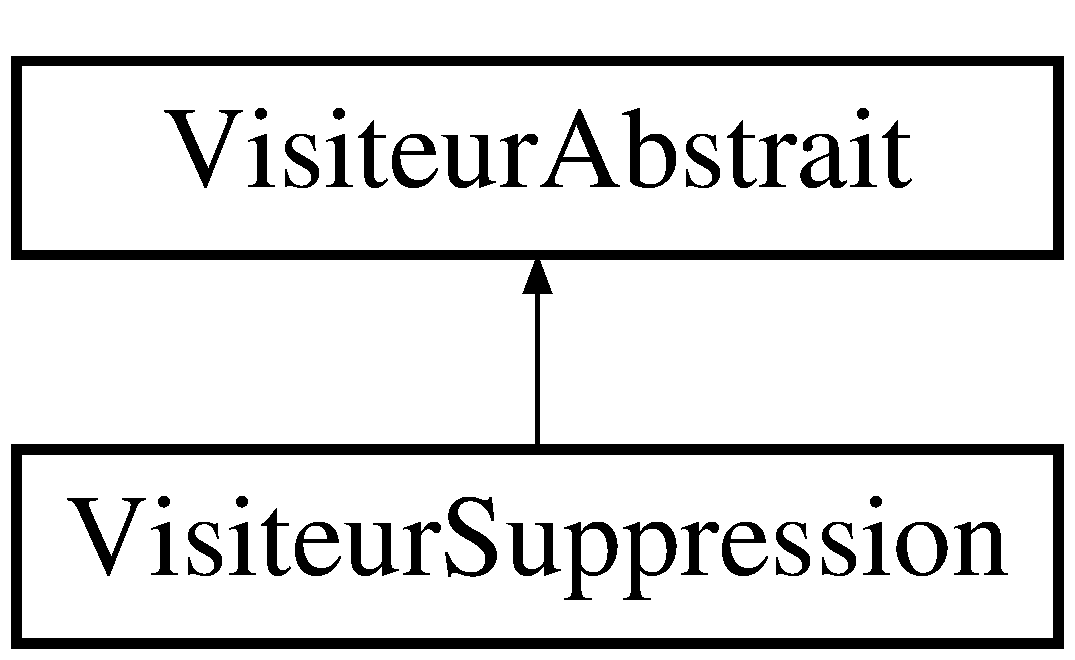
\includegraphics[height=2.000000cm]{class_visiteur_suppression}
\end{center}
\end{figure}
\subsection*{Public Member Functions}
\begin{DoxyCompactItemize}
\item 
\hyperlink{group__inf2990_ga77790339ddd453ed30dffccef8934373}{Visiteur\+Suppression} ()
\begin{DoxyCompactList}\small\item\em Constructeur. \end{DoxyCompactList}\item 
\hyperlink{group__inf2990_ga609bdf7e42165bdfa8d4c4d816c2b71d}{$\sim$\+Visiteur\+Suppression} ()
\begin{DoxyCompactList}\small\item\em Destructeur. \end{DoxyCompactList}\item 
virtual void \hyperlink{group__inf2990_gae0fb11ee5dcb5859fd4e163b685b637f}{visiter} (\hyperlink{class_noeud_composite}{Noeud\+Composite} $\ast$)
\begin{DoxyCompactList}\small\item\em visites des differents noeuds \end{DoxyCompactList}\item 
virtual void \hyperlink{group__inf2990_ga16f8a5baaf97984aa643548b3d7fdb77}{visiter} (\hyperlink{class_noeud_maillet}{Noeud\+Maillet} $\ast$)
\item 
virtual void \hyperlink{group__inf2990_ga9c2fa9629828ea966b7f8823f3fc27f1}{visiter} (\hyperlink{class_noeud_muret}{Noeud\+Muret} $\ast$)
\item 
virtual void \hyperlink{group__inf2990_ga44d65975bdbc7e3d83171694ad8bd49f}{visiter} (\hyperlink{class_noeud_portail}{Noeud\+Portail} $\ast$)
\item 
virtual void \hyperlink{group__inf2990_ga583a45169e345e2262f8a572c32e7822}{visiter} (\hyperlink{class_noeud_rondelle}{Noeud\+Rondelle} $\ast$)
\item 
virtual void \hyperlink{group__inf2990_gae84d0ab8c7eb74a325d3da3a3629d0b3}{visiter} (\hyperlink{class_noeud_table}{Noeud\+Table} $\ast$)
\item 
virtual void \hyperlink{group__inf2990_ga16d27e0e09fbdfde27639965c71c415c}{visiter} (\hyperlink{class_noeud_bonus_accelerateur}{Noeud\+Bonus\+Accelerateur} $\ast$)
\end{DoxyCompactItemize}
\subsection*{Additional Inherited Members}


The documentation for this class was generated from the following files\+:\begin{DoxyCompactItemize}
\item 
Sources/\+D\+L\+L/\hyperlink{_visiteur_suppression_8h}{Visiteur\+Suppression.\+h}\item 
Sources/\+D\+L\+L/\hyperlink{_visiteur_suppression_8cpp}{Visiteur\+Suppression.\+cpp}\end{DoxyCompactItemize}

\chapter{File Documentation}
\hypertarget{_facade_modele_8cpp}{}\section{C\+:/\+Users/\+Steven/\+Documents/\+Poly/\+I\+N\+F2990/inf2990-\/06/\+Cadriciel\+\_\+2016-\/3\+\_\+\+Etudiants/\+Cadriciel/\+Sources/\+D\+L\+L/\+Application/\+Facade\+Modele.cpp File Reference}
\label{_facade_modele_8cpp}\index{C\+:/\+Users/\+Steven/\+Documents/\+Poly/\+I\+N\+F2990/inf2990-\/06/\+Cadriciel\+\_\+2016-\/3\+\_\+\+Etudiants/\+Cadriciel/\+Sources/\+D\+L\+L/\+Application/\+Facade\+Modele.\+cpp@{C\+:/\+Users/\+Steven/\+Documents/\+Poly/\+I\+N\+F2990/inf2990-\/06/\+Cadriciel\+\_\+2016-\/3\+\_\+\+Etudiants/\+Cadriciel/\+Sources/\+D\+L\+L/\+Application/\+Facade\+Modele.\+cpp}}
{\ttfamily \#include $<$windows.\+h$>$}\newline
{\ttfamily \#include $<$cassert$>$}\newline
{\ttfamily \#include \char`\"{}G\+L/glew.\+h\char`\"{}}\newline
{\ttfamily \#include \char`\"{}Free\+Image.\+h\char`\"{}}\newline
{\ttfamily \#include \char`\"{}Facade\+Modele.\+h\char`\"{}}\newline
{\ttfamily \#include \char`\"{}Vue\+Ortho.\+h\char`\"{}}\newline
{\ttfamily \#include \char`\"{}Camera.\+h\char`\"{}}\newline
{\ttfamily \#include \char`\"{}Projection.\+h\char`\"{}}\newline
{\ttfamily \#include \char`\"{}Utilitaire.\+h\char`\"{}}\newline
{\ttfamily \#include \char`\"{}Aide\+G\+L.\+h\char`\"{}}\newline
{\ttfamily \#include \char`\"{}Arbre\+Rendu\+I\+N\+F2990.\+h\char`\"{}}\newline
{\ttfamily \#include \char`\"{}Config\+Scene.\+h\char`\"{}}\newline
{\ttfamily \#include \char`\"{}Compteur\+Affichage.\+h\char`\"{}}\newline
{\ttfamily \#include $<$vector$>$}\newline
{\ttfamily \#include \char`\"{}tinyxml2.\+h\char`\"{}}\newline
{\ttfamily \#include \char`\"{}glm/glm.\+hpp\char`\"{}}\newline
{\ttfamily \#include \char`\"{}glm/gtc/type\+\_\+ptr.\+hpp\char`\"{}}\newline
{\ttfamily \#include \char`\"{}../\+Visiteur\+Selection.\+h\char`\"{}}\newline


\subsection{Detailed Description}
\begin{DoxyAuthor}{Author}
Martin Bisson 
\end{DoxyAuthor}
\begin{DoxyDate}{Date}
2007-\/05-\/22 
\end{DoxyDate}
\begin{DoxyVersion}{Version}
1.\+0 
\end{DoxyVersion}

\hypertarget{_facade_modele_8h}{}\section{Sources/\+D\+L\+L/\+Application/\+Facade\+Modele.h File Reference}
\label{_facade_modele_8h}\index{Sources/\+D\+L\+L/\+Application/\+Facade\+Modele.\+h@{Sources/\+D\+L\+L/\+Application/\+Facade\+Modele.\+h}}
{\ttfamily \#include $<$windows.\+h$>$}\newline
{\ttfamily \#include $<$string$>$}\newline
{\ttfamily \#include \char`\"{}../\+Visiteur\+Selection.\+h\char`\"{}}\newline
{\ttfamily \#include \char`\"{}Noeud\+Table.\+h\char`\"{}}\newline
{\ttfamily \#include \char`\"{}../\+Visiteur\+Duplication.\+h\char`\"{}}\newline
{\ttfamily \#include \char`\"{}../\+Visiteur\+Deplacement.\+h\char`\"{}}\newline
{\ttfamily \#include \char`\"{}../\+Visiteur\+Rotation.\+h\char`\"{}}\newline
{\ttfamily \#include \char`\"{}../\+Visiteur\+Suppression.\+h\char`\"{}}\newline
{\ttfamily \#include \char`\"{}../\+Visiteur\+Ecriture\+X\+M\+L.\+h\char`\"{}}\newline
{\ttfamily \#include \char`\"{}../\+Visiteur\+Echelle.\+h\char`\"{}}\newline
{\ttfamily \#include \char`\"{}../\+Visiteur\+Collision.\+h\char`\"{}}\newline
{\ttfamily \#include \char`\"{}Partie.\+h\char`\"{}}\newline
{\ttfamily \#include \char`\"{}Tournoi.\+h\char`\"{}}\newline
{\ttfamily \#include \char`\"{}../\+Profil\+Virtuel.\+h\char`\"{}}\newline
\subsection*{Classes}
\begin{DoxyCompactItemize}
\item 
class \hyperlink{class_facade_modele}{Facade\+Modele}
\begin{DoxyCompactList}\small\item\em Classe qui constitue une interface (une fa�ade) sur l\textquotesingle{}ensemble du mod�le et des classes qui le composent. \end{DoxyCompactList}\end{DoxyCompactItemize}


\subsection{Detailed Description}
\begin{DoxyAuthor}{Author}
D\+GI 
\end{DoxyAuthor}
\begin{DoxyDate}{Date}
2005-\/06-\/15 
\end{DoxyDate}
\begin{DoxyVersion}{Version}
1.\+0 
\end{DoxyVersion}

\hypertarget{_arbre_rendu_8cpp}{}\section{Sources/\+D\+L\+L/\+Arbre/\+Arbre\+Rendu.cpp File Reference}
\label{_arbre_rendu_8cpp}\index{Sources/\+D\+L\+L/\+Arbre/\+Arbre\+Rendu.\+cpp@{Sources/\+D\+L\+L/\+Arbre/\+Arbre\+Rendu.\+cpp}}
{\ttfamily \#include \char`\"{}Arbre\+Rendu.\+h\char`\"{}}\newline
{\ttfamily \#include \char`\"{}Usine\+Noeud.\+h\char`\"{}}\newline
{\ttfamily \#include \char`\"{}Noeud\+Abstrait.\+h\char`\"{}}\newline
{\ttfamily \#include \char`\"{}G\+L/glew.\+h\char`\"{}}\newline


\subsection{Detailed Description}
\begin{DoxyAuthor}{Author}
Martin Bisson 
\end{DoxyAuthor}
\begin{DoxyDate}{Date}
2007-\/01-\/28 
\end{DoxyDate}

\hypertarget{_arbre_rendu_8h}{}\section{Sources/\+D\+L\+L/\+Arbre/\+Arbre\+Rendu.h File Reference}
\label{_arbre_rendu_8h}\index{Sources/\+D\+L\+L/\+Arbre/\+Arbre\+Rendu.\+h@{Sources/\+D\+L\+L/\+Arbre/\+Arbre\+Rendu.\+h}}
{\ttfamily \#include \char`\"{}Noeud\+Composite.\+h\char`\"{}}\newline
{\ttfamily \#include \char`\"{}tinyxml2.\+h\char`\"{}}\newline
{\ttfamily \#include $<$string$>$}\newline
{\ttfamily \#include $<$map$>$}\newline
\subsection*{Classes}
\begin{DoxyCompactItemize}
\item 
class \hyperlink{class_arbre_rendu}{Arbre\+Rendu}
\begin{DoxyCompactList}\small\item\em Classe d\textquotesingle{}arbre de rendu qui contient la racine de l\textquotesingle{}arbre de rendu avec les usines qui permettent d\textquotesingle{}ajouter des noeuds � cet arbre. \end{DoxyCompactList}\end{DoxyCompactItemize}


\subsection{Detailed Description}
\begin{DoxyAuthor}{Author}
Martin Bisson 
\end{DoxyAuthor}
\begin{DoxyDate}{Date}
2007-\/01-\/28 
\end{DoxyDate}
\begin{DoxyVersion}{Version}
1.\+0 
\end{DoxyVersion}

\hypertarget{_arbre_rendu_i_n_f2990_8cpp}{}\section{C\+:/\+Users/\+Steven/\+Documents/\+Poly/\+I\+N\+F2990/inf2990-\/06/\+Cadriciel\+\_\+2016-\/3\+\_\+\+Etudiants/\+Cadriciel/\+Sources/\+D\+L\+L/\+Arbre/\+Arbre\+Rendu\+I\+N\+F2990.cpp File Reference}
\label{_arbre_rendu_i_n_f2990_8cpp}\index{C\+:/\+Users/\+Steven/\+Documents/\+Poly/\+I\+N\+F2990/inf2990-\/06/\+Cadriciel\+\_\+2016-\/3\+\_\+\+Etudiants/\+Cadriciel/\+Sources/\+D\+L\+L/\+Arbre/\+Arbre\+Rendu\+I\+N\+F2990.\+cpp@{C\+:/\+Users/\+Steven/\+Documents/\+Poly/\+I\+N\+F2990/inf2990-\/06/\+Cadriciel\+\_\+2016-\/3\+\_\+\+Etudiants/\+Cadriciel/\+Sources/\+D\+L\+L/\+Arbre/\+Arbre\+Rendu\+I\+N\+F2990.\+cpp}}
{\ttfamily \#include \char`\"{}Arbre\+Rendu\+I\+N\+F2990.\+h\char`\"{}}\newline
{\ttfamily \#include \char`\"{}Usines/\+Usine\+Noeud.\+h\char`\"{}}\newline
{\ttfamily \#include \char`\"{}Usine\+Noeud\+Portail.\+h\char`\"{}}\newline
{\ttfamily \#include \char`\"{}Usine\+Noeud\+Table.\+h\char`\"{}}\newline
{\ttfamily \#include \char`\"{}Usine\+Noeud\+Maillet1.\+h\char`\"{}}\newline
{\ttfamily \#include \char`\"{}Usine\+Noeud\+Maillet\+Virtuel.\+h\char`\"{}}\newline
{\ttfamily \#include \char`\"{}Usine\+Noeud\+Muret.\+h\char`\"{}}\newline
{\ttfamily \#include \char`\"{}Usine\+Noeud\+Bonus\+Accelerateur.\+h\char`\"{}}\newline
{\ttfamily \#include \char`\"{}Usine\+Noeud\+Rondelle.\+h\char`\"{}}\newline
{\ttfamily \#include \char`\"{}Usine\+Noeud\+Cercle.\+h\char`\"{}}\newline
{\ttfamily \#include \char`\"{}Facade\+Modele.\+h\char`\"{}}\newline
{\ttfamily \#include \char`\"{}Etat\+Open\+G\+L.\+h\char`\"{}}\newline
{\ttfamily \#include \char`\"{}Noeuds/\+Noeud\+Types.\+h\char`\"{}}\newline
{\ttfamily \#include $<$cmath$>$}\newline


\subsection{Detailed Description}
\begin{DoxyAuthor}{Author}
Martin Bisson 
\end{DoxyAuthor}
\begin{DoxyDate}{Date}
2007-\/03-\/23 
\end{DoxyDate}
\begin{DoxyVersion}{Version}
1.\+0 
\end{DoxyVersion}

\hypertarget{_arbre_rendu_i_n_f2990_8h}{}\section{Sources/\+D\+L\+L/\+Arbre/\+Arbre\+Rendu\+I\+N\+F2990.h File Reference}
\label{_arbre_rendu_i_n_f2990_8h}\index{Sources/\+D\+L\+L/\+Arbre/\+Arbre\+Rendu\+I\+N\+F2990.\+h@{Sources/\+D\+L\+L/\+Arbre/\+Arbre\+Rendu\+I\+N\+F2990.\+h}}
{\ttfamily \#include \char`\"{}Arbre\+Rendu.\+h\char`\"{}}\newline
{\ttfamily \#include $<$map$>$}\newline
{\ttfamily \#include $<$string$>$}\newline
\subsection*{Classes}
\begin{DoxyCompactItemize}
\item 
class \hyperlink{class_arbre_rendu_i_n_f2990}{Arbre\+Rendu\+I\+N\+F2990}
\begin{DoxyCompactList}\small\item\em Classe qui représente l\textquotesingle{}arbre de rendu spécifique au projet de I\+N\+F2990. \end{DoxyCompactList}\end{DoxyCompactItemize}


\subsection{Detailed Description}
\begin{DoxyAuthor}{Author}
Martin Bisson 
\end{DoxyAuthor}
\begin{DoxyDate}{Date}
2007-\/03-\/23 
\end{DoxyDate}
\begin{DoxyVersion}{Version}
1.\+0 
\end{DoxyVersion}

\hypertarget{_noeud_abstrait_8cpp}{}\section{C\+:/\+Users/\+Steven/\+Documents/\+Poly/\+I\+N\+F2990/inf2990-\/06/\+Cadriciel\+\_\+2016-\/3\+\_\+\+Etudiants/\+Cadriciel/\+Sources/\+D\+L\+L/\+Arbre/\+Noeuds/\+Noeud\+Abstrait.cpp File Reference}
\label{_noeud_abstrait_8cpp}\index{C\+:/\+Users/\+Steven/\+Documents/\+Poly/\+I\+N\+F2990/inf2990-\/06/\+Cadriciel\+\_\+2016-\/3\+\_\+\+Etudiants/\+Cadriciel/\+Sources/\+D\+L\+L/\+Arbre/\+Noeuds/\+Noeud\+Abstrait.\+cpp@{C\+:/\+Users/\+Steven/\+Documents/\+Poly/\+I\+N\+F2990/inf2990-\/06/\+Cadriciel\+\_\+2016-\/3\+\_\+\+Etudiants/\+Cadriciel/\+Sources/\+D\+L\+L/\+Arbre/\+Noeuds/\+Noeud\+Abstrait.\+cpp}}
{\ttfamily \#include \char`\"{}Noeud\+Abstrait.\+h\char`\"{}}\newline
{\ttfamily \#include \char`\"{}Utilitaire.\+h\char`\"{}}\newline


\subsection{Detailed Description}
\begin{DoxyAuthor}{Author}
D\+G\+I-\/2990 
\end{DoxyAuthor}
\begin{DoxyDate}{Date}
2007-\/01-\/24 
\end{DoxyDate}

\hypertarget{_noeud_abstrait_8h}{}\section{Sources/\+D\+L\+L/\+Arbre/\+Noeuds/\+Noeud\+Abstrait.h File Reference}
\label{_noeud_abstrait_8h}\index{Sources/\+D\+L\+L/\+Arbre/\+Noeuds/\+Noeud\+Abstrait.\+h@{Sources/\+D\+L\+L/\+Arbre/\+Noeuds/\+Noeud\+Abstrait.\+h}}
{\ttfamily \#include \char`\"{}G\+L/glew.\+h\char`\"{}}\newline
{\ttfamily \#include $<$string$>$}\newline
{\ttfamily \#include $<$vector$>$}\newline
{\ttfamily \#include \char`\"{}glm\textbackslash{}glm.\+hpp\char`\"{}}\newline
{\ttfamily \#include \char`\"{}glm\textbackslash{}gtc\textbackslash{}matrix\+\_\+transform.\+hpp\char`\"{}}\newline
{\ttfamily \#include \char`\"{}../\+Visiteur\+Abstrait.\+h\char`\"{}}\newline
\subsection*{Classes}
\begin{DoxyCompactItemize}
\item 
class \hyperlink{class_noeud_abstrait}{Noeud\+Abstrait}
\begin{DoxyCompactList}\small\item\em Classe de base du patron composite utilis�e pour cr�er l\textquotesingle{}arbre de rendu. \end{DoxyCompactList}\end{DoxyCompactItemize}
\subsection*{Namespaces}
\begin{DoxyCompactItemize}
\item 
 \hyperlink{namespacemodele}{modele}
\begin{DoxyCompactList}\small\item\em D�clarations avanc�es pour contenir un pointeur vers un mod�le3D et son storage. \end{DoxyCompactList}\end{DoxyCompactItemize}


\subsection{Detailed Description}
\begin{DoxyAuthor}{Author}
D\+G\+I-\/\+I\+N\+F2990 
\end{DoxyAuthor}
\begin{DoxyDate}{Date}
2007-\/01-\/24 
\end{DoxyDate}
\begin{DoxyVersion}{Version}
1.\+0 
\end{DoxyVersion}

\hypertarget{_noeud_araignee_8cpp}{}\section{Sources/\+D\+L\+L/\+Arbre/\+Noeuds/\+Noeud\+Araignee.cpp File Reference}
\label{_noeud_araignee_8cpp}\index{Sources/\+D\+L\+L/\+Arbre/\+Noeuds/\+Noeud\+Araignee.\+cpp@{Sources/\+D\+L\+L/\+Arbre/\+Noeuds/\+Noeud\+Araignee.\+cpp}}
{\ttfamily \#include \char`\"{}Noeud\+Araignee.\+h\char`\"{}}\newline
{\ttfamily \#include \char`\"{}Utilitaire.\+h\char`\"{}}\newline
{\ttfamily \#include \char`\"{}G\+L/glew.\+h\char`\"{}}\newline
{\ttfamily \#include $<$cmath$>$}\newline
{\ttfamily \#include \char`\"{}Modele3\+D.\+h\char`\"{}}\newline
{\ttfamily \#include \char`\"{}Open\+G\+L\+\_\+\+V\+B\+O.\+h\char`\"{}}\newline


\subsection{Detailed Description}
\begin{DoxyAuthor}{Author}
Julien Gascon-\/\+Samson 
\end{DoxyAuthor}
\begin{DoxyDate}{Date}
2011-\/05-\/19 
\end{DoxyDate}
\begin{DoxyVersion}{Version}
1.\+0 
\end{DoxyVersion}

\hypertarget{_noeud_araignee_8h}{}\section{C\+:/\+Users/\+Steven/\+Documents/\+Poly/\+I\+N\+F2990/inf2990-\/06/\+Cadriciel\+\_\+2016-\/3\+\_\+\+Etudiants/\+Cadriciel/\+Sources/\+D\+L\+L/\+Arbre/\+Noeuds/\+Noeud\+Araignee.h File Reference}
\label{_noeud_araignee_8h}\index{C\+:/\+Users/\+Steven/\+Documents/\+Poly/\+I\+N\+F2990/inf2990-\/06/\+Cadriciel\+\_\+2016-\/3\+\_\+\+Etudiants/\+Cadriciel/\+Sources/\+D\+L\+L/\+Arbre/\+Noeuds/\+Noeud\+Araignee.\+h@{C\+:/\+Users/\+Steven/\+Documents/\+Poly/\+I\+N\+F2990/inf2990-\/06/\+Cadriciel\+\_\+2016-\/3\+\_\+\+Etudiants/\+Cadriciel/\+Sources/\+D\+L\+L/\+Arbre/\+Noeuds/\+Noeud\+Araignee.\+h}}
{\ttfamily \#include \char`\"{}Noeud\+Composite.\+h\char`\"{}}\newline
{\ttfamily \#include \char`\"{}G\+L/glew.\+h\char`\"{}}\newline
\subsection*{Classes}
\begin{DoxyCompactItemize}
\item 
class \hyperlink{class_noeud_araignee}{Noeud\+Araignee}
\begin{DoxyCompactList}\small\item\em Classe qui repr�sente un exemple de noeud de l\textquotesingle{}arbre de rendu. \end{DoxyCompactList}\end{DoxyCompactItemize}


\subsection{Detailed Description}
\begin{DoxyAuthor}{Author}
Julien Gascon-\/\+Samson 
\end{DoxyAuthor}
\begin{DoxyDate}{Date}
2011-\/05-\/19 
\end{DoxyDate}
\begin{DoxyVersion}{Version}
1.\+0 
\end{DoxyVersion}

\hypertarget{_noeud_bonus_accelerateur_8cpp}{}\section{Sources/\+D\+L\+L/\+Arbre/\+Noeuds/\+Noeud\+Bonus\+Accelerateur.cpp File Reference}
\label{_noeud_bonus_accelerateur_8cpp}\index{Sources/\+D\+L\+L/\+Arbre/\+Noeuds/\+Noeud\+Bonus\+Accelerateur.\+cpp@{Sources/\+D\+L\+L/\+Arbre/\+Noeuds/\+Noeud\+Bonus\+Accelerateur.\+cpp}}
{\ttfamily \#include \char`\"{}Noeud\+Bonus\+Accelerateur.\+h\char`\"{}}\newline
{\ttfamily \#include \char`\"{}Utilitaire.\+h\char`\"{}}\newline
{\ttfamily \#include \char`\"{}G\+L/glew.\+h\char`\"{}}\newline
{\ttfamily \#include $<$cmath$>$}\newline
{\ttfamily \#include \char`\"{}Modele3\+D.\+h\char`\"{}}\newline
{\ttfamily \#include \char`\"{}Open\+G\+L\+\_\+\+V\+B\+O.\+h\char`\"{}}\newline


\subsection{Detailed Description}
\begin{DoxyAuthor}{Author}
equipe06 
\end{DoxyAuthor}
\begin{DoxyDate}{Date}
2016-\/09-\/07 
\end{DoxyDate}
\begin{DoxyVersion}{Version}
1.\+0 
\end{DoxyVersion}

\hypertarget{_noeud_bonus_accelerateur_8h}{}\section{Sources/\+D\+L\+L/\+Arbre/\+Noeuds/\+Noeud\+Bonus\+Accelerateur.h File Reference}
\label{_noeud_bonus_accelerateur_8h}\index{Sources/\+D\+L\+L/\+Arbre/\+Noeuds/\+Noeud\+Bonus\+Accelerateur.\+h@{Sources/\+D\+L\+L/\+Arbre/\+Noeuds/\+Noeud\+Bonus\+Accelerateur.\+h}}
{\ttfamily \#include \char`\"{}Noeud\+Composite.\+h\char`\"{}}\newline
{\ttfamily \#include \char`\"{}G\+L/glew.\+h\char`\"{}}\newline
\subsection*{Classes}
\begin{DoxyCompactItemize}
\item 
class \hyperlink{class_noeud_bonus_accelerateur}{Noeud\+Bonus\+Accelerateur}
\begin{DoxyCompactList}\small\item\em Classe qui repr�sente un exemple de noeud de l\textquotesingle{}arbre de rendu. \end{DoxyCompactList}\end{DoxyCompactItemize}


\subsection{Detailed Description}
\begin{DoxyAuthor}{Author}
equipe06 
\end{DoxyAuthor}
\begin{DoxyDate}{Date}
2016-\/09-\/07 
\end{DoxyDate}
\begin{DoxyVersion}{Version}
1.\+0 
\end{DoxyVersion}

\hypertarget{_noeud_cercle_8cpp}{}\section{Sources/\+D\+L\+L/\+Arbre/\+Noeuds/\+Noeud\+Cercle.cpp File Reference}
\label{_noeud_cercle_8cpp}\index{Sources/\+D\+L\+L/\+Arbre/\+Noeuds/\+Noeud\+Cercle.\+cpp@{Sources/\+D\+L\+L/\+Arbre/\+Noeuds/\+Noeud\+Cercle.\+cpp}}
{\ttfamily \#include \char`\"{}Noeud\+Cercle.\+h\char`\"{}}\newline
{\ttfamily \#include \char`\"{}Utilitaire.\+h\char`\"{}}\newline
{\ttfamily \#include \char`\"{}G\+L/glew.\+h\char`\"{}}\newline
{\ttfamily \#include $<$cmath$>$}\newline
{\ttfamily \#include \char`\"{}Facade\+Modele.\+h\char`\"{}}\newline
{\ttfamily \#include \char`\"{}Modele3\+D.\+h\char`\"{}}\newline
{\ttfamily \#include \char`\"{}Open\+G\+L\+\_\+\+V\+B\+O.\+h\char`\"{}}\newline


\subsection{Detailed Description}
\begin{DoxyAuthor}{Author}
equipe06 
\end{DoxyAuthor}
\begin{DoxyDate}{Date}
2016-\/09-\/07 
\end{DoxyDate}
\begin{DoxyVersion}{Version}
1.\+0 
\end{DoxyVersion}

\hypertarget{_noeud_cercle_8h}{}\section{Sources/\+D\+L\+L/\+Arbre/\+Noeuds/\+Noeud\+Cercle.h File Reference}
\label{_noeud_cercle_8h}\index{Sources/\+D\+L\+L/\+Arbre/\+Noeuds/\+Noeud\+Cercle.\+h@{Sources/\+D\+L\+L/\+Arbre/\+Noeuds/\+Noeud\+Cercle.\+h}}
{\ttfamily \#include \char`\"{}Noeud\+Composite.\+h\char`\"{}}\newline
{\ttfamily \#include \char`\"{}G\+L/glew.\+h\char`\"{}}\newline
\subsection*{Classes}
\begin{DoxyCompactItemize}
\item 
class \hyperlink{class_noeud_cercle}{Noeud\+Cercle}
\begin{DoxyCompactList}\small\item\em Classe qui repr�sente un exemple de noeud de l\textquotesingle{}arbre de rendu. \end{DoxyCompactList}\end{DoxyCompactItemize}


\subsection{Detailed Description}
\begin{DoxyAuthor}{Author}
equipe06 
\end{DoxyAuthor}
\begin{DoxyDate}{Date}
2016-\/09-\/07 
\end{DoxyDate}
\begin{DoxyVersion}{Version}
1.\+0 
\end{DoxyVersion}

\hypertarget{_noeud_composite_8cpp}{}\section{C\+:/\+Users/\+Steven/\+Documents/\+Poly/\+I\+N\+F2990/inf2990-\/06/\+Cadriciel\+\_\+2016-\/3\+\_\+\+Etudiants/\+Cadriciel/\+Sources/\+D\+L\+L/\+Arbre/\+Noeuds/\+Noeud\+Composite.cpp File Reference}
\label{_noeud_composite_8cpp}\index{C\+:/\+Users/\+Steven/\+Documents/\+Poly/\+I\+N\+F2990/inf2990-\/06/\+Cadriciel\+\_\+2016-\/3\+\_\+\+Etudiants/\+Cadriciel/\+Sources/\+D\+L\+L/\+Arbre/\+Noeuds/\+Noeud\+Composite.\+cpp@{C\+:/\+Users/\+Steven/\+Documents/\+Poly/\+I\+N\+F2990/inf2990-\/06/\+Cadriciel\+\_\+2016-\/3\+\_\+\+Etudiants/\+Cadriciel/\+Sources/\+D\+L\+L/\+Arbre/\+Noeuds/\+Noeud\+Composite.\+cpp}}
{\ttfamily \#include \char`\"{}Noeud\+Composite.\+h\char`\"{}}\newline
{\ttfamily \#include $<$cassert$>$}\newline


\subsection{Detailed Description}
\begin{DoxyAuthor}{Author}
D\+G\+I-\/2990 
\end{DoxyAuthor}
\begin{DoxyDate}{Date}
2007-\/01-\/25 
\end{DoxyDate}

\hypertarget{_noeud_composite_8h}{}\section{Sources/\+D\+L\+L/\+Arbre/\+Noeuds/\+Noeud\+Composite.h File Reference}
\label{_noeud_composite_8h}\index{Sources/\+D\+L\+L/\+Arbre/\+Noeuds/\+Noeud\+Composite.\+h@{Sources/\+D\+L\+L/\+Arbre/\+Noeuds/\+Noeud\+Composite.\+h}}
{\ttfamily \#include \char`\"{}Noeud\+Abstrait.\+h\char`\"{}}\newline
{\ttfamily \#include $<$vector$>$}\newline
\subsection*{Classes}
\begin{DoxyCompactItemize}
\item 
class \hyperlink{class_noeud_composite}{Noeud\+Composite}
\begin{DoxyCompactList}\small\item\em Implantation d\textquotesingle{}un noeud du patron composite qui peut poss�der des enfants. \end{DoxyCompactList}\end{DoxyCompactItemize}
\subsection*{Typedefs}
\begin{DoxyCompactItemize}
\item 
using \hyperlink{group__inf2990_gae5f081f07546f0b622ee841a2d6e5a0d}{conteneur\+\_\+enfants} = std\+::vector$<$ \hyperlink{class_noeud_abstrait}{Noeud\+Abstrait} $\ast$ $>$
\begin{DoxyCompactList}\small\item\em Le choix du conteneur pour les enfants. \end{DoxyCompactList}\end{DoxyCompactItemize}


\subsection{Detailed Description}
\begin{DoxyAuthor}{Author}
D\+G\+I-\/\+I\+N\+F2990 
\end{DoxyAuthor}
\begin{DoxyDate}{Date}
2007-\/01-\/25 
\end{DoxyDate}
\begin{DoxyVersion}{Version}
1.\+0 
\end{DoxyVersion}

\hypertarget{_noeud_cone_cube_8cpp}{}\section{C\+:/\+Users/\+Steven/\+Documents/\+Poly/\+I\+N\+F2990/inf2990-\/06/\+Cadriciel\+\_\+2016-\/3\+\_\+\+Etudiants/\+Cadriciel/\+Sources/\+D\+L\+L/\+Arbre/\+Noeuds/\+Noeud\+Cone\+Cube.cpp File Reference}
\label{_noeud_cone_cube_8cpp}\index{C\+:/\+Users/\+Steven/\+Documents/\+Poly/\+I\+N\+F2990/inf2990-\/06/\+Cadriciel\+\_\+2016-\/3\+\_\+\+Etudiants/\+Cadriciel/\+Sources/\+D\+L\+L/\+Arbre/\+Noeuds/\+Noeud\+Cone\+Cube.\+cpp@{C\+:/\+Users/\+Steven/\+Documents/\+Poly/\+I\+N\+F2990/inf2990-\/06/\+Cadriciel\+\_\+2016-\/3\+\_\+\+Etudiants/\+Cadriciel/\+Sources/\+D\+L\+L/\+Arbre/\+Noeuds/\+Noeud\+Cone\+Cube.\+cpp}}
{\ttfamily \#include \char`\"{}Noeud\+Cone\+Cube.\+h\char`\"{}}\newline
{\ttfamily \#include \char`\"{}G\+L/glew.\+h\char`\"{}}\newline
{\ttfamily \#include $<$cmath$>$}\newline
{\ttfamily \#include \char`\"{}Modele3\+D.\+h\char`\"{}}\newline
{\ttfamily \#include \char`\"{}Open\+G\+L\+\_\+\+V\+B\+O.\+h\char`\"{}}\newline
{\ttfamily \#include \char`\"{}Utilitaire.\+h\char`\"{}}\newline


\subsection{Detailed Description}
\begin{DoxyAuthor}{Author}
Julien Gascon-\/\+Samson 
\end{DoxyAuthor}
\begin{DoxyDate}{Date}
2011-\/05-\/19 
\end{DoxyDate}
\begin{DoxyVersion}{Version}
1.\+0 
\end{DoxyVersion}

\hypertarget{_noeud_cone_cube_8h}{}\section{Sources/\+D\+L\+L/\+Arbre/\+Noeuds/\+Noeud\+Cone\+Cube.h File Reference}
\label{_noeud_cone_cube_8h}\index{Sources/\+D\+L\+L/\+Arbre/\+Noeuds/\+Noeud\+Cone\+Cube.\+h@{Sources/\+D\+L\+L/\+Arbre/\+Noeuds/\+Noeud\+Cone\+Cube.\+h}}
{\ttfamily \#include \char`\"{}Noeud\+Abstrait.\+h\char`\"{}}\newline
{\ttfamily \#include \char`\"{}G\+L/glew.\+h\char`\"{}}\newline
\subsection*{Classes}
\begin{DoxyCompactItemize}
\item 
class \hyperlink{class_noeud_cone_cube}{Noeud\+Cone\+Cube}
\begin{DoxyCompactList}\small\item\em Classe qui repr�sente un exemple de noeud de l\textquotesingle{}arbre de rendu. \end{DoxyCompactList}\end{DoxyCompactItemize}


\subsection{Detailed Description}
\begin{DoxyAuthor}{Author}
Julien Gascon-\/\+Samson 
\end{DoxyAuthor}
\begin{DoxyDate}{Date}
2011-\/05-\/19 
\end{DoxyDate}
\begin{DoxyVersion}{Version}
1.\+0 
\end{DoxyVersion}

\hypertarget{_noeud_joueur_8cpp}{}\section{C\+:/\+Users/\+Steven/\+Documents/\+Poly/\+I\+N\+F2990/inf2990-\/06/\+Cadriciel\+\_\+2016-\/3\+\_\+\+Etudiants/\+Cadriciel/\+Sources/\+D\+L\+L/\+Arbre/\+Noeuds/\+Noeud\+Joueur.cpp File Reference}
\label{_noeud_joueur_8cpp}\index{C\+:/\+Users/\+Steven/\+Documents/\+Poly/\+I\+N\+F2990/inf2990-\/06/\+Cadriciel\+\_\+2016-\/3\+\_\+\+Etudiants/\+Cadriciel/\+Sources/\+D\+L\+L/\+Arbre/\+Noeuds/\+Noeud\+Joueur.\+cpp@{C\+:/\+Users/\+Steven/\+Documents/\+Poly/\+I\+N\+F2990/inf2990-\/06/\+Cadriciel\+\_\+2016-\/3\+\_\+\+Etudiants/\+Cadriciel/\+Sources/\+D\+L\+L/\+Arbre/\+Noeuds/\+Noeud\+Joueur.\+cpp}}
{\ttfamily \#include \char`\"{}Noeud\+Joueur.\+h\char`\"{}}\newline


\subsection{Detailed Description}
\begin{DoxyAuthor}{Author}
equipe06 
\end{DoxyAuthor}
\begin{DoxyDate}{Date}
2016-\/10-\/21 
\end{DoxyDate}
\begin{DoxyVersion}{Version}
1.\+0 
\end{DoxyVersion}

\hypertarget{_noeud_joueur_8h}{}\section{Sources/\+D\+L\+L/\+Arbre/\+Noeuds/\+Noeud\+Joueur.h File Reference}
\label{_noeud_joueur_8h}\index{Sources/\+D\+L\+L/\+Arbre/\+Noeuds/\+Noeud\+Joueur.\+h@{Sources/\+D\+L\+L/\+Arbre/\+Noeuds/\+Noeud\+Joueur.\+h}}
{\ttfamily \#include \char`\"{}Noeud\+Composite.\+h\char`\"{}}\newline
{\ttfamily \#include \char`\"{}Noeud\+Rondelle.\+h\char`\"{}}\newline
\subsection*{Classes}
\begin{DoxyCompactItemize}
\item 
class \hyperlink{class_noeud_joueur}{Noeud\+Joueur}
\end{DoxyCompactItemize}


\subsection{Detailed Description}
\begin{DoxyAuthor}{Author}
Equipe 6 
\end{DoxyAuthor}
\begin{DoxyDate}{Date}
2016-\/11-\/10 
\end{DoxyDate}
\begin{DoxyVersion}{Version}
1.\+0 
\end{DoxyVersion}

\hypertarget{_noeud_maillet_8cpp}{}\section{C\+:/\+Users/\+Steven/\+Documents/\+Poly/\+I\+N\+F2990/inf2990-\/06/\+Cadriciel\+\_\+2016-\/3\+\_\+\+Etudiants/\+Cadriciel/\+Sources/\+D\+L\+L/\+Arbre/\+Noeuds/\+Noeud\+Maillet.cpp File Reference}
\label{_noeud_maillet_8cpp}\index{C\+:/\+Users/\+Steven/\+Documents/\+Poly/\+I\+N\+F2990/inf2990-\/06/\+Cadriciel\+\_\+2016-\/3\+\_\+\+Etudiants/\+Cadriciel/\+Sources/\+D\+L\+L/\+Arbre/\+Noeuds/\+Noeud\+Maillet.\+cpp@{C\+:/\+Users/\+Steven/\+Documents/\+Poly/\+I\+N\+F2990/inf2990-\/06/\+Cadriciel\+\_\+2016-\/3\+\_\+\+Etudiants/\+Cadriciel/\+Sources/\+D\+L\+L/\+Arbre/\+Noeuds/\+Noeud\+Maillet.\+cpp}}
{\ttfamily \#include \char`\"{}Noeud\+Maillet.\+h\char`\"{}}\newline
{\ttfamily \#include \char`\"{}Utilitaire.\+h\char`\"{}}\newline
{\ttfamily \#include \char`\"{}Facade\+Modele.\+h\char`\"{}}\newline
{\ttfamily \#include \char`\"{}G\+L/glew.\+h\char`\"{}}\newline
{\ttfamily \#include $<$cmath$>$}\newline
{\ttfamily \#include \char`\"{}Modele3\+D.\+h\char`\"{}}\newline
{\ttfamily \#include \char`\"{}Open\+G\+L\+\_\+\+V\+B\+O.\+h\char`\"{}}\newline


\subsection{Detailed Description}
\begin{DoxyAuthor}{Author}
equipe06 
\end{DoxyAuthor}
\begin{DoxyDate}{Date}
2016-\/09-\/07 
\end{DoxyDate}
\begin{DoxyVersion}{Version}
1.\+0 
\end{DoxyVersion}

\hypertarget{_noeud_maillet_8h}{}\section{C\+:/\+Users/\+Steven/\+Documents/\+Poly/\+I\+N\+F2990/inf2990-\/06/\+Cadriciel\+\_\+2016-\/3\+\_\+\+Etudiants/\+Cadriciel/\+Sources/\+D\+L\+L/\+Arbre/\+Noeuds/\+Noeud\+Maillet.h File Reference}
\label{_noeud_maillet_8h}\index{C\+:/\+Users/\+Steven/\+Documents/\+Poly/\+I\+N\+F2990/inf2990-\/06/\+Cadriciel\+\_\+2016-\/3\+\_\+\+Etudiants/\+Cadriciel/\+Sources/\+D\+L\+L/\+Arbre/\+Noeuds/\+Noeud\+Maillet.\+h@{C\+:/\+Users/\+Steven/\+Documents/\+Poly/\+I\+N\+F2990/inf2990-\/06/\+Cadriciel\+\_\+2016-\/3\+\_\+\+Etudiants/\+Cadriciel/\+Sources/\+D\+L\+L/\+Arbre/\+Noeuds/\+Noeud\+Maillet.\+h}}
{\ttfamily \#include \char`\"{}Noeud\+Composite.\+h\char`\"{}}\newline
{\ttfamily \#include \char`\"{}G\+L/glew.\+h\char`\"{}}\newline
\subsection*{Classes}
\begin{DoxyCompactItemize}
\item 
class \hyperlink{class_noeud_maillet}{Noeud\+Maillet}
\begin{DoxyCompactList}\small\item\em Classe qui repr�sente un exemple de noeud de l\textquotesingle{}arbre de rendu. \end{DoxyCompactList}\end{DoxyCompactItemize}


\subsection{Detailed Description}
\begin{DoxyAuthor}{Author}
equipe06 
\end{DoxyAuthor}
\begin{DoxyDate}{Date}
2016-\/09-\/07 
\end{DoxyDate}
\begin{DoxyVersion}{Version}
1.\+0 
\end{DoxyVersion}

\hypertarget{_noeud_maillet_virtuel_8cpp}{}\section{Sources/\+D\+L\+L/\+Arbre/\+Noeuds/\+Noeud\+Maillet\+Virtuel.cpp File Reference}
\label{_noeud_maillet_virtuel_8cpp}\index{Sources/\+D\+L\+L/\+Arbre/\+Noeuds/\+Noeud\+Maillet\+Virtuel.\+cpp@{Sources/\+D\+L\+L/\+Arbre/\+Noeuds/\+Noeud\+Maillet\+Virtuel.\+cpp}}
{\ttfamily \#include \char`\"{}Noeud\+Maillet\+Virtuel.\+h\char`\"{}}\newline
{\ttfamily \#include \char`\"{}Utilitaire.\+h\char`\"{}}\newline
{\ttfamily \#include \char`\"{}Facade\+Modele.\+h\char`\"{}}\newline
{\ttfamily \#include \char`\"{}G\+L/glew.\+h\char`\"{}}\newline
{\ttfamily \#include $<$cmath$>$}\newline
{\ttfamily \#include \char`\"{}Modele3\+D.\+h\char`\"{}}\newline
{\ttfamily \#include \char`\"{}Open\+G\+L\+\_\+\+V\+B\+O.\+h\char`\"{}}\newline
\subsection*{Macros}
\begin{DoxyCompactItemize}
\item 
\#define {\bfseries V\+I\+T\+E\+S\+S\+E\+\_\+\+M\+AX}~5.\+0
\item 
\#define {\bfseries V\+I\+T\+E\+S\+S\+E\+\_\+\+M\+A\+X\+\_\+\+M\+A\+I\+L\+L\+ET}~20.\+0
\item 
\#define {\bfseries D\+I\+S\+T\+A\+N\+C\+E\+\_\+\+D\+U\+\_\+\+B\+UT}~7.\+0
\end{DoxyCompactItemize}


\subsection{Detailed Description}
\begin{DoxyAuthor}{Author}
equipe06 
\end{DoxyAuthor}
\begin{DoxyDate}{Date}
2016-\/09-\/07 
\end{DoxyDate}
\begin{DoxyVersion}{Version}
1.\+0 
\end{DoxyVersion}

\hypertarget{_noeud_maillet_virtuel_8h}{}\section{Sources/\+D\+L\+L/\+Arbre/\+Noeuds/\+Noeud\+Maillet\+Virtuel.h File Reference}
\label{_noeud_maillet_virtuel_8h}\index{Sources/\+D\+L\+L/\+Arbre/\+Noeuds/\+Noeud\+Maillet\+Virtuel.\+h@{Sources/\+D\+L\+L/\+Arbre/\+Noeuds/\+Noeud\+Maillet\+Virtuel.\+h}}
{\ttfamily \#include \char`\"{}Noeud\+Composite.\+h\char`\"{}}\newline
{\ttfamily \#include \char`\"{}G\+L/glew.\+h\char`\"{}}\newline
{\ttfamily \#include \char`\"{}glm/gtx/norm.\+hpp\char`\"{}}\newline
{\ttfamily \#include \char`\"{}Noeud\+Rondelle.\+h\char`\"{}}\newline
\subsection*{Classes}
\begin{DoxyCompactItemize}
\item 
class \hyperlink{class_noeud_maillet_virtuel}{Noeud\+Maillet\+Virtuel}
\end{DoxyCompactItemize}


\subsection{Detailed Description}
\begin{DoxyAuthor}{Author}
equipe06 
\end{DoxyAuthor}
\begin{DoxyDate}{Date}
2016-\/09-\/07 
\end{DoxyDate}
\begin{DoxyVersion}{Version}
1.\+0 
\end{DoxyVersion}

\hypertarget{_noeud_muret_8h}{}\section{Sources/\+D\+L\+L/\+Arbre/\+Noeuds/\+Noeud\+Muret.h File Reference}
\label{_noeud_muret_8h}\index{Sources/\+D\+L\+L/\+Arbre/\+Noeuds/\+Noeud\+Muret.\+h@{Sources/\+D\+L\+L/\+Arbre/\+Noeuds/\+Noeud\+Muret.\+h}}
{\ttfamily \#include \char`\"{}Noeud\+Composite.\+h\char`\"{}}\newline
{\ttfamily \#include \char`\"{}G\+L/glew.\+h\char`\"{}}\newline
\subsection*{Classes}
\begin{DoxyCompactItemize}
\item 
class \hyperlink{class_noeud_muret}{Noeud\+Muret}
\end{DoxyCompactItemize}


\subsection{Detailed Description}
\begin{DoxyAuthor}{Author}
equipe06 
\end{DoxyAuthor}
\begin{DoxyDate}{Date}
2016-\/09-\/07 
\end{DoxyDate}
\begin{DoxyVersion}{Version}
1.\+0 
\end{DoxyVersion}

\hypertarget{_noeud_portail_8cpp}{}\section{Sources/\+D\+L\+L/\+Arbre/\+Noeuds/\+Noeud\+Portail.cpp File Reference}
\label{_noeud_portail_8cpp}\index{Sources/\+D\+L\+L/\+Arbre/\+Noeuds/\+Noeud\+Portail.\+cpp@{Sources/\+D\+L\+L/\+Arbre/\+Noeuds/\+Noeud\+Portail.\+cpp}}
{\ttfamily \#include \char`\"{}Noeud\+Portail.\+h\char`\"{}}\newline
{\ttfamily \#include \char`\"{}Utilitaire.\+h\char`\"{}}\newline
{\ttfamily \#include \char`\"{}G\+L/glew.\+h\char`\"{}}\newline
{\ttfamily \#include $<$cmath$>$}\newline
{\ttfamily \#include $<$iostream$>$}\newline
{\ttfamily \#include \char`\"{}Modele3\+D.\+h\char`\"{}}\newline
{\ttfamily \#include \char`\"{}Open\+G\+L\+\_\+\+V\+B\+O.\+h\char`\"{}}\newline
{\ttfamily \#include \char`\"{}Facade\+Modele.\+h\char`\"{}}\newline
{\ttfamily \#include \char`\"{}glm/glm.\+hpp\char`\"{}}\newline
\subsection*{Variables}
\begin{DoxyCompactItemize}
\item 
const float {\bfseries P\+R\+O\+P\+O\+R\+T\+I\+O\+N\+\_\+\+A\+T\+T\+R\+A\+C\+T\+I\+ON} = 5.\+0
\item 
const float {\bfseries V\+I\+T\+E\+S\+S\+E\+\_\+\+R\+O\+T\+A\+T\+I\+O\+N\+\_\+\+M\+I\+N\+I\+M\+AL} = 10.\+6f
\item 
const float {\bfseries V\+I\+T\+E\+S\+S\+E\+\_\+\+R\+O\+T\+A\+T\+I\+O\+N\+\_\+\+M\+A\+X\+I\+M\+AL} = 25.\+0f
\end{DoxyCompactItemize}


\subsection{Detailed Description}
\begin{DoxyAuthor}{Author}
equipe06 
\end{DoxyAuthor}
\begin{DoxyDate}{Date}
2016-\/09-\/07 
\end{DoxyDate}
\begin{DoxyVersion}{Version}
1.\+0 
\end{DoxyVersion}

\hypertarget{_noeud_portail_8h}{}\section{Sources/\+D\+L\+L/\+Arbre/\+Noeuds/\+Noeud\+Portail.h File Reference}
\label{_noeud_portail_8h}\index{Sources/\+D\+L\+L/\+Arbre/\+Noeuds/\+Noeud\+Portail.\+h@{Sources/\+D\+L\+L/\+Arbre/\+Noeuds/\+Noeud\+Portail.\+h}}
{\ttfamily \#include \char`\"{}Noeud\+Composite.\+h\char`\"{}}\newline
{\ttfamily \#include \char`\"{}G\+L/glew.\+h\char`\"{}}\newline
\subsection*{Classes}
\begin{DoxyCompactItemize}
\item 
class \hyperlink{class_noeud_portail}{Noeud\+Portail}
\end{DoxyCompactItemize}


\subsection{Detailed Description}
\begin{DoxyAuthor}{Author}
equipe06 
\end{DoxyAuthor}
\begin{DoxyDate}{Date}
2016-\/09-\/07 
\end{DoxyDate}
\begin{DoxyVersion}{Version}
1.\+0 
\end{DoxyVersion}

\hypertarget{_noeud_rondelle_8cpp}{}\section{Sources/\+D\+L\+L/\+Arbre/\+Noeuds/\+Noeud\+Rondelle.cpp File Reference}
\label{_noeud_rondelle_8cpp}\index{Sources/\+D\+L\+L/\+Arbre/\+Noeuds/\+Noeud\+Rondelle.\+cpp@{Sources/\+D\+L\+L/\+Arbre/\+Noeuds/\+Noeud\+Rondelle.\+cpp}}
{\ttfamily \#include \char`\"{}Noeud\+Rondelle.\+h\char`\"{}}\newline
{\ttfamily \#include \char`\"{}Utilitaire.\+h\char`\"{}}\newline
{\ttfamily \#include \char`\"{}Aide\+Collision.\+h\char`\"{}}\newline
{\ttfamily \#include \char`\"{}Facade\+Modele.\+h\char`\"{}}\newline
{\ttfamily \#include \char`\"{}G\+L/glew.\+h\char`\"{}}\newline
{\ttfamily \#include $<$cmath$>$}\newline
{\ttfamily \#include $<$iostream$>$}\newline
{\ttfamily \#include \char`\"{}Modele3\+D.\+h\char`\"{}}\newline
{\ttfamily \#include \char`\"{}Open\+G\+L\+\_\+\+V\+B\+O.\+h\char`\"{}}\newline
\subsection*{Variables}
\begin{DoxyCompactItemize}
\item 
const double {\bfseries V\+I\+T\+E\+S\+S\+E\+\_\+\+D\+E\+P\+L\+A\+C\+E\+M\+E\+N\+T\+\_\+\+M\+I\+N\+I\+M\+AL} = 0.\+0
\item 
const double {\bfseries V\+I\+T\+E\+S\+S\+E\+\_\+\+D\+E\+P\+L\+A\+C\+E\+M\+E\+N\+T\+\_\+\+M\+A\+X\+I\+M\+AL} = 2.\+0
\end{DoxyCompactItemize}


\subsection{Detailed Description}
\begin{DoxyAuthor}{Author}
equipe06 
\end{DoxyAuthor}
\begin{DoxyDate}{Date}
2016-\/09-\/07 
\end{DoxyDate}
\begin{DoxyVersion}{Version}
1.\+0 
\end{DoxyVersion}

\hypertarget{_noeud_rondelle_8h}{}\section{C\+:/\+Users/\+Steven/\+Documents/\+Poly/\+I\+N\+F2990/inf2990-\/06/\+Cadriciel\+\_\+2016-\/3\+\_\+\+Etudiants/\+Cadriciel/\+Sources/\+D\+L\+L/\+Arbre/\+Noeuds/\+Noeud\+Rondelle.h File Reference}
\label{_noeud_rondelle_8h}\index{C\+:/\+Users/\+Steven/\+Documents/\+Poly/\+I\+N\+F2990/inf2990-\/06/\+Cadriciel\+\_\+2016-\/3\+\_\+\+Etudiants/\+Cadriciel/\+Sources/\+D\+L\+L/\+Arbre/\+Noeuds/\+Noeud\+Rondelle.\+h@{C\+:/\+Users/\+Steven/\+Documents/\+Poly/\+I\+N\+F2990/inf2990-\/06/\+Cadriciel\+\_\+2016-\/3\+\_\+\+Etudiants/\+Cadriciel/\+Sources/\+D\+L\+L/\+Arbre/\+Noeuds/\+Noeud\+Rondelle.\+h}}
{\ttfamily \#include \char`\"{}Noeud\+Composite.\+h\char`\"{}}\newline
{\ttfamily \#include \char`\"{}G\+L/glew.\+h\char`\"{}}\newline
{\ttfamily \#include \char`\"{}Noeud\+Table.\+h\char`\"{}}\newline
{\ttfamily \#include \char`\"{}Utilitaire.\+h\char`\"{}}\newline
\subsection*{Classes}
\begin{DoxyCompactItemize}
\item 
class \hyperlink{class_noeud_rondelle}{Noeud\+Rondelle}
\begin{DoxyCompactList}\small\item\em Classe qui repr�sente un exemple de noeud de l\textquotesingle{}arbre de rendu. \end{DoxyCompactList}\end{DoxyCompactItemize}


\subsection{Detailed Description}
\begin{DoxyAuthor}{Author}
equipe06 
\end{DoxyAuthor}
\begin{DoxyDate}{Date}
2016-\/09-\/07 
\end{DoxyDate}
\begin{DoxyVersion}{Version}
1.\+0 
\end{DoxyVersion}

\hypertarget{_noeud_table_8cpp}{}\section{Sources/\+D\+L\+L/\+Arbre/\+Noeuds/\+Noeud\+Table.cpp File Reference}
\label{_noeud_table_8cpp}\index{Sources/\+D\+L\+L/\+Arbre/\+Noeuds/\+Noeud\+Table.\+cpp@{Sources/\+D\+L\+L/\+Arbre/\+Noeuds/\+Noeud\+Table.\+cpp}}
{\ttfamily \#include \char`\"{}Noeud\+Table.\+h\char`\"{}}\newline
{\ttfamily \#include \char`\"{}../\+Arbre/\+Texture.\+h\char`\"{}}\newline
{\ttfamily \#include $<$glm/glm.\+hpp$>$}\newline
{\ttfamily \#include $<$glm/gtc/type\+\_\+ptr.\+hpp$>$}\newline
\subsection*{Macros}
\begin{DoxyCompactItemize}
\item 
\hypertarget{_noeud_table_8cpp_af8a8ca9ee1dd7cd0c2a170f57a2b2e0b}{}\label{_noeud_table_8cpp_af8a8ca9ee1dd7cd0c2a170f57a2b2e0b} 
\#define {\bfseries pos0}~glm\+::value\+\_\+ptr(glm\+::vec3(vue\+Projection $\ast$ glm\+::vec4(sommet\+T\+\_\+\mbox{[}0\mbox{]},1)))
\item 
\hypertarget{_noeud_table_8cpp_a30d0b6d3e1055b0035c1724ea29d8a0c}{}\label{_noeud_table_8cpp_a30d0b6d3e1055b0035c1724ea29d8a0c} 
\#define {\bfseries pos1}~glm\+::value\+\_\+ptr(glm\+::vec3(vue\+Projection $\ast$ glm\+::vec4(sommet\+T\+\_\+\mbox{[}1\mbox{]},1)))
\item 
\hypertarget{_noeud_table_8cpp_a1df8d7ebc951fb3d5eea0074588e0ced}{}\label{_noeud_table_8cpp_a1df8d7ebc951fb3d5eea0074588e0ced} 
\#define {\bfseries pos2}~glm\+::value\+\_\+ptr(glm\+::vec3(vue\+Projection $\ast$ glm\+::vec4(sommet\+T\+\_\+\mbox{[}2\mbox{]},1)))
\item 
\hypertarget{_noeud_table_8cpp_a84947dbd95d68e9b0d9b28fc4f1fbd33}{}\label{_noeud_table_8cpp_a84947dbd95d68e9b0d9b28fc4f1fbd33} 
\#define {\bfseries pos3}~glm\+::value\+\_\+ptr(glm\+::vec3(vue\+Projection $\ast$ glm\+::vec4(sommet\+T\+\_\+\mbox{[}3\mbox{]},1)))
\item 
\hypertarget{_noeud_table_8cpp_a4d37ed7ca3bfa9a156939ebca5c3096c}{}\label{_noeud_table_8cpp_a4d37ed7ca3bfa9a156939ebca5c3096c} 
\#define {\bfseries pos4}~glm\+::value\+\_\+ptr(glm\+::vec3(vue\+Projection $\ast$ glm\+::vec4(sommet\+T\+\_\+\mbox{[}4\mbox{]},1)))
\item 
\hypertarget{_noeud_table_8cpp_abfce2cb27d81174bcfce8be9869e2111}{}\label{_noeud_table_8cpp_abfce2cb27d81174bcfce8be9869e2111} 
\#define {\bfseries pos5}~glm\+::value\+\_\+ptr(glm\+::vec3(vue\+Projection $\ast$ glm\+::vec4(sommet\+T\+\_\+\mbox{[}5\mbox{]},1)))
\item 
\hypertarget{_noeud_table_8cpp_a5d2c9056ef4a9224cf09d9e5fb36a688}{}\label{_noeud_table_8cpp_a5d2c9056ef4a9224cf09d9e5fb36a688} 
\#define {\bfseries pos6}~glm\+::value\+\_\+ptr(glm\+::vec3(vue\+Projection $\ast$ glm\+::vec4(sommet\+T\+\_\+\mbox{[}6\mbox{]},1)))
\item 
\hypertarget{_noeud_table_8cpp_a142496fa72407742c5010273454c6af1}{}\label{_noeud_table_8cpp_a142496fa72407742c5010273454c6af1} 
\#define {\bfseries pos7}~glm\+::value\+\_\+ptr(glm\+::vec3(vue\+Projection $\ast$ glm\+::vec4(sommet\+T\+\_\+\mbox{[}7\mbox{]},1)))
\item 
\hypertarget{_noeud_table_8cpp_a560d75a32ccaf5265159d0fd65d54eaa}{}\label{_noeud_table_8cpp_a560d75a32ccaf5265159d0fd65d54eaa} 
\#define {\bfseries pos8}~glm\+::value\+\_\+ptr(glm\+::vec3(vue\+Projection $\ast$ glm\+::vec4(sommet\+T\+\_\+\mbox{[}8\mbox{]},1)))
\item 
\hypertarget{_noeud_table_8cpp_a6107b97c9d18f6410bbe4e8e489708a3}{}\label{_noeud_table_8cpp_a6107b97c9d18f6410bbe4e8e489708a3} 
\#define {\bfseries B\+U\+T11}~glm\+::value\+\_\+ptr(glm\+::vec3(vue\+Projection $\ast$ glm\+::vec4(sommet\+T\+\_\+\mbox{[}5\mbox{]}.x, sommet\+T\+\_\+\mbox{[}5\mbox{]}.y+10, 0, 1)))
\item 
\hypertarget{_noeud_table_8cpp_a9cdd0d3efa6ed3512afa1f6b9145b2e5}{}\label{_noeud_table_8cpp_a9cdd0d3efa6ed3512afa1f6b9145b2e5} 
\#define {\bfseries B\+U\+T12}~glm\+::value\+\_\+ptr(glm\+::vec3(vue\+Projection $\ast$ glm\+::vec4(sommet\+T\+\_\+\mbox{[}5\mbox{]}.x, sommet\+T\+\_\+\mbox{[}5\mbox{]}.y-\/10, 0, 1)))
\item 
\hypertarget{_noeud_table_8cpp_ad942b36eeee6b636f693b1f9ab1c89e9}{}\label{_noeud_table_8cpp_ad942b36eeee6b636f693b1f9ab1c89e9} 
\#define {\bfseries B\+U\+T21}~glm\+::value\+\_\+ptr(glm\+::vec3(vue\+Projection $\ast$ glm\+::vec4(sommet\+T\+\_\+\mbox{[}1\mbox{]}.x, sommet\+T\+\_\+\mbox{[}1\mbox{]}.y+10, 0, 1)))
\item 
\hypertarget{_noeud_table_8cpp_a3f46aafc8af612deac5573c51bb1444d}{}\label{_noeud_table_8cpp_a3f46aafc8af612deac5573c51bb1444d} 
\#define {\bfseries B\+U\+T22}~glm\+::value\+\_\+ptr(glm\+::vec3(vue\+Projection $\ast$ glm\+::vec4(sommet\+T\+\_\+\mbox{[}1\mbox{]}.x, sommet\+T\+\_\+\mbox{[}1\mbox{]}.y-\/10, 0, 1)))
\end{DoxyCompactItemize}

\hypertarget{_noeud_table_8h}{}\section{Sources/\+D\+L\+L/\+Arbre/\+Noeuds/\+Noeud\+Table.h File Reference}
\label{_noeud_table_8h}\index{Sources/\+D\+L\+L/\+Arbre/\+Noeuds/\+Noeud\+Table.\+h@{Sources/\+D\+L\+L/\+Arbre/\+Noeuds/\+Noeud\+Table.\+h}}
{\ttfamily \#include \char`\"{}Noeud\+Composite.\+h\char`\"{}}\newline
{\ttfamily \#include \char`\"{}G\+L/glew.\+h\char`\"{}}\newline
{\ttfamily \#include \char`\"{}Noeud\+Maillet.\+h\char`\"{}}\newline
{\ttfamily \#include \char`\"{}Noeud\+Rondelle.\+h\char`\"{}}\newline
{\ttfamily \#include \char`\"{}Utilitaire.\+h\char`\"{}}\newline
\subsection*{Classes}
\begin{DoxyCompactItemize}
\item 
class \hyperlink{class_noeud_table}{Noeud\+Table}
\begin{DoxyCompactList}\small\item\em Classe qui représente un exemple de noeud de l\textquotesingle{}arbre de rendu. \end{DoxyCompactList}\end{DoxyCompactItemize}


\subsection{Detailed Description}
\begin{DoxyAuthor}{Author}
equipe06 
\end{DoxyAuthor}
\begin{DoxyDate}{Date}
2016-\/09-\/07 
\end{DoxyDate}
\begin{DoxyVersion}{Version}
1.\+0 
\end{DoxyVersion}

\hypertarget{_texture_8cpp}{}\section{Sources/\+D\+L\+L/\+Arbre/\+Texture.cpp File Reference}
\label{_texture_8cpp}\index{Sources/\+D\+L\+L/\+Arbre/\+Texture.\+cpp@{Sources/\+D\+L\+L/\+Arbre/\+Texture.\+cpp}}
{\ttfamily \#include \char`\"{}Texture.\+h\char`\"{}}\newline
{\ttfamily \#include $<$windows.\+h$>$}\newline
{\ttfamily \#include $<$G\+L/gl.\+h$>$}\newline
\subsection*{Macros}
\begin{DoxyCompactItemize}
\item 
\#define {\bfseries G\+L\+\_\+\+C\+L\+A\+M\+P\+\_\+\+T\+O\+\_\+\+E\+D\+GE}~0x812F
\end{DoxyCompactItemize}


\subsection{Detailed Description}
\begin{DoxyAuthor}{Author}
Mathieu Kavalec 
\end{DoxyAuthor}
\begin{DoxyDate}{Date}
2013-\/02-\/10 
\end{DoxyDate}
\begin{DoxyVersion}{Version}
1.\+0 
\end{DoxyVersion}

\hypertarget{_usine_noeud_8h}{}\section{Sources/\+D\+L\+L/\+Arbre/\+Usines/\+Usine\+Noeud.h File Reference}
\label{_usine_noeud_8h}\index{Sources/\+D\+L\+L/\+Arbre/\+Usines/\+Usine\+Noeud.\+h@{Sources/\+D\+L\+L/\+Arbre/\+Usines/\+Usine\+Noeud.\+h}}
{\ttfamily \#include $<$type\+\_\+traits$>$}\newline
{\ttfamily \#include $<$string$>$}\newline
{\ttfamily \#include \char`\"{}Modele3\+D.\+h\char`\"{}}\newline
{\ttfamily \#include \char`\"{}Open\+G\+L\+\_\+\+V\+B\+O.\+h\char`\"{}}\newline
{\ttfamily \#include \char`\"{}tinyxml2.\+h\char`\"{}}\newline
\subsection*{Classes}
\begin{DoxyCompactItemize}
\item 
class \hyperlink{class_usine_abstraite}{Usine\+Abstraite}
\begin{DoxyCompactList}\small\item\em Classe de base abstraite des usines qui seront utilis�es pour cr�er les diff�rents noeuds de l\textquotesingle{}arbre de rendu. \end{DoxyCompactList}\end{DoxyCompactItemize}


\subsection{Detailed Description}
\begin{DoxyAuthor}{Author}
Martin Bisson 
\end{DoxyAuthor}
\begin{DoxyDate}{Date}
2007-\/01-\/28 
\end{DoxyDate}
\begin{DoxyVersion}{Version}
1.\+0 
\end{DoxyVersion}

\hypertarget{_usine_noeud_portail_8h}{}\section{Sources/\+D\+L\+L/\+Arbre/\+Usines/\+Usine\+Noeud\+Portail.h File Reference}
\label{_usine_noeud_portail_8h}\index{Sources/\+D\+L\+L/\+Arbre/\+Usines/\+Usine\+Noeud\+Portail.\+h@{Sources/\+D\+L\+L/\+Arbre/\+Usines/\+Usine\+Noeud\+Portail.\+h}}
{\ttfamily \#include \char`\"{}Usine\+Noeud.\+h\char`\"{}}\newline
{\ttfamily \#include \char`\"{}Noeud\+Portail.\+h\char`\"{}}\newline
{\ttfamily \#include \char`\"{}Modele3\+D.\+h\char`\"{}}\newline
{\ttfamily \#include \char`\"{}Open\+G\+L\+\_\+\+V\+B\+O.\+h\char`\"{}}\newline
{\ttfamily \#include \char`\"{}tinyxml2.\+h\char`\"{}}\newline
\subsection*{Classes}
\begin{DoxyCompactItemize}
\item 
class \hyperlink{class_usine_noeud_portail}{Usine\+Noeud\+Portail}
\begin{DoxyCompactList}\small\item\em Classe qui repr�sente une usine capable de cr�er des noeuds de type \hyperlink{class_noeud_portail}{Noeud\+Portail}. \end{DoxyCompactList}\end{DoxyCompactItemize}


\subsection{Detailed Description}
\begin{DoxyAuthor}{Author}
equipe06 
\end{DoxyAuthor}
\begin{DoxyDate}{Date}
2016-\/09-\/30 
\end{DoxyDate}
\begin{DoxyVersion}{Version}
1.\+0 
\end{DoxyVersion}

\hypertarget{_usine_noeud_table_8h}{}\section{Sources/\+D\+L\+L/\+Arbre/\+Usines/\+Usine\+Noeud\+Table.h File Reference}
\label{_usine_noeud_table_8h}\index{Sources/\+D\+L\+L/\+Arbre/\+Usines/\+Usine\+Noeud\+Table.\+h@{Sources/\+D\+L\+L/\+Arbre/\+Usines/\+Usine\+Noeud\+Table.\+h}}
{\ttfamily \#include \char`\"{}Usine\+Noeud.\+h\char`\"{}}\newline
{\ttfamily \#include \char`\"{}Noeud\+Table.\+h\char`\"{}}\newline
{\ttfamily \#include \char`\"{}Modele3\+D.\+h\char`\"{}}\newline
{\ttfamily \#include \char`\"{}Open\+G\+L\+\_\+\+V\+B\+O.\+h\char`\"{}}\newline
{\ttfamily \#include \char`\"{}tinyxml2.\+h\char`\"{}}\newline
\subsection*{Classes}
\begin{DoxyCompactItemize}
\item 
class \hyperlink{class_usine_noeud_table}{Usine\+Noeud\+Table}
\end{DoxyCompactItemize}


\subsection{Detailed Description}
\begin{DoxyAuthor}{Author}
equipe06 
\end{DoxyAuthor}
\begin{DoxyDate}{Date}
2016-\/09-\/30 
\end{DoxyDate}
\begin{DoxyVersion}{Version}
1.\+0 
\end{DoxyVersion}

\hypertarget{_config_scene_8cpp}{}\section{Sources/\+D\+L\+L/\+Configuration/\+Config\+Scene.cpp File Reference}
\label{_config_scene_8cpp}\index{Sources/\+D\+L\+L/\+Configuration/\+Config\+Scene.\+cpp@{Sources/\+D\+L\+L/\+Configuration/\+Config\+Scene.\+cpp}}
{\ttfamily \#include \char`\"{}Config\+Scene.\+h\char`\"{}}\newline
{\ttfamily \#include $<$iostream$>$}\newline
\subsection*{Functions}
\begin{DoxyCompactItemize}
\item 
{\bfseries S\+I\+N\+G\+L\+E\+T\+O\+N\+\_\+\+D\+E\+C\+L\+A\+R\+A\+T\+I\+O\+N\+\_\+\+C\+PP} (\hyperlink{class_config_scene}{Config\+Scene})
\end{DoxyCompactItemize}


\subsection{Detailed Description}
\begin{DoxyAuthor}{Author}
Jean-\/\+Fran�ois P�russe 
\end{DoxyAuthor}
\begin{DoxyDate}{Date}
2007-\/01-\/10 
\end{DoxyDate}
\begin{DoxyVersion}{Version}
1.\+0 
\end{DoxyVersion}

\hypertarget{_config_scene_8h}{}\section{Sources/\+D\+L\+L/\+Configuration/\+Config\+Scene.h File Reference}
\label{_config_scene_8h}\index{Sources/\+D\+L\+L/\+Configuration/\+Config\+Scene.\+h@{Sources/\+D\+L\+L/\+Configuration/\+Config\+Scene.\+h}}
{\ttfamily \#include \char`\"{}Singleton.\+h\char`\"{}}\newline
{\ttfamily \#include \char`\"{}tinyxml2.\+h\char`\"{}}\newline
\subsection*{Classes}
\begin{DoxyCompactItemize}
\item 
class \hyperlink{class_config_scene}{Config\+Scene}
\begin{DoxyCompactList}\small\item\em Les variables de configuration de la classe C\+Scene. C\textquotesingle{}est une classe singleton. \end{DoxyCompactList}\end{DoxyCompactItemize}


\subsection{Detailed Description}
\begin{DoxyAuthor}{Author}
Jean-\/\+Fran�ois P�russe 
\end{DoxyAuthor}
\begin{DoxyDate}{Date}
2007-\/01-\/10 
\end{DoxyDate}
\begin{DoxyVersion}{Version}
1.\+0 
\end{DoxyVersion}

\hypertarget{_facade_interface_native_8cpp}{}\section{Sources/\+D\+L\+L/\+Interface/\+Facade\+Interface\+Native.cpp File Reference}
\label{_facade_interface_native_8cpp}\index{Sources/\+D\+L\+L/\+Interface/\+Facade\+Interface\+Native.\+cpp@{Sources/\+D\+L\+L/\+Interface/\+Facade\+Interface\+Native.\+cpp}}
{\ttfamily \#include \char`\"{}Facade\+Interface\+Native.\+h\char`\"{}}\newline
{\ttfamily \#include \char`\"{}Facade\+Modele.\+h\char`\"{}}\newline
{\ttfamily \#include \char`\"{}glm\textbackslash{}glm.\+hpp\char`\"{}}\newline
{\ttfamily \#include \char`\"{}Aide\+G\+L.\+h\char`\"{}}\newline
{\ttfamily \#include \char`\"{}Vue.\+h\char`\"{}}\newline
{\ttfamily \#include \char`\"{}Arbre\+Rendu\+I\+N\+F2990.\+h\char`\"{}}\newline
{\ttfamily \#include \char`\"{}Compteur\+Affichage.\+h\char`\"{}}\newline
{\ttfamily \#include \char`\"{}Banc\+Tests.\+h\char`\"{}}\newline
\subsection*{Functions}
\begin{DoxyCompactItemize}
\item 
\hyperlink{group__inf2990_gab7f5f39b522334aa53af43ba21a16719}{\+\_\+\+\_\+declspec} (dllexport) void \+\_\+\+\_\+cdecl initialiser\+Open\+GL(int $\ast$handle)
\end{DoxyCompactItemize}
\subsection*{Variables}
\begin{DoxyCompactItemize}
\item 
int {\bfseries hauteur}
\item 
int {\bfseries x}
\item 
int int {\bfseries y}
\item 
int {\bfseries y1}
\item 
int {\bfseries posY}
\item 
int bool {\bfseries attribuer}
\item 
int {\bfseries pointY}
\item 
int bool {\bfseries selection\+Unique}
\item 
int int int {\bfseries largeur}
\item 
double {\bfseries deplacementY}
\end{DoxyCompactItemize}


\subsection{Detailed Description}
\begin{DoxyAuthor}{Author}
I\+N\+F2990 
\end{DoxyAuthor}
\begin{DoxyDate}{Date}
2014-\/08-\/16 
\end{DoxyDate}

\hypertarget{_facade_interface_native_8h}{}\section{Sources/\+D\+L\+L/\+Interface/\+Facade\+Interface\+Native.h File Reference}
\label{_facade_interface_native_8h}\index{Sources/\+D\+L\+L/\+Interface/\+Facade\+Interface\+Native.\+h@{Sources/\+D\+L\+L/\+Interface/\+Facade\+Interface\+Native.\+h}}
{\ttfamily \#include $<$string$>$}\newline
\subsection*{Functions}
\begin{DoxyCompactItemize}
\item 
\hyperlink{group__inf2990_gab7f5f39b522334aa53af43ba21a16719}{\+\_\+\+\_\+declspec} (dllexport) void \+\_\+\+\_\+cdecl initialiser\+Open\+GL(int $\ast$handle)
\end{DoxyCompactItemize}
\subsection*{Variables}
\begin{DoxyCompactItemize}
\item 
int {\bfseries hauteur}
\item 
int {\bfseries x}
\item 
int int {\bfseries y}
\item 
int {\bfseries y1}
\item 
int {\bfseries posY}
\item 
int bool {\bfseries attribuer}
\item 
int {\bfseries pointY}
\item 
int int int {\bfseries largeur}
\item 
int int int bool {\bfseries selection\+Unique}
\item 
double {\bfseries deplacementY}
\item 
bool {\bfseries peut\+Afficher\+Collision}
\item 
bool bool {\bfseries peut\+Afficher\+Vitesse\+Rondelle}
\item 
bool bool bool {\bfseries peut\+Afficher\+Eclairage}
\item 
bool bool bool bool {\bfseries peut\+Afficher\+Attraction\+Portail}
\item 
bool bool bool bool int {\bfseries nb\+Buts}
\item 
bool bool bool bool int char $\ast$ {\bfseries haut}
\item 
bool bool bool bool int char char $\ast$ {\bfseries bas}
\item 
bool bool bool bool int char char char $\ast$ {\bfseries gauche}
\item 
bool bool bool bool int char char char char $\ast$ {\bfseries droite}
\item 
bool bool bool bool int char char char char bool {\bfseries est\+Virtuel}
\item 
int {\bfseries vitesse}
\item 
int int {\bfseries passivite}
\item 
{\bfseries bool}
\item 
char $\ast$ {\bfseries nom2}
\item 
bool {\bfseries j1}
\item 
bool char $\ast$ {\bfseries nom1}
\item 
bool char bool {\bfseries j2}
\item 
bool char bool char bool {\bfseries j3}
\item 
bool char bool char bool char $\ast$ {\bfseries nom3}
\item 
bool char bool char bool char bool {\bfseries j4}
\item 
bool char bool char bool char bool char $\ast$ {\bfseries nom4}
\end{DoxyCompactItemize}


\subsection{Detailed Description}
\begin{DoxyAuthor}{Author}
I\+N\+F2990 
\end{DoxyAuthor}
\begin{DoxyDate}{Date}
2014-\/08-\/16 
\end{DoxyDate}

\hypertarget{_interface_configuration_8h}{}\section{C\+:/\+Users/\+Steven/\+Documents/\+Poly/\+I\+N\+F2990/inf2990-\/06/\+Cadriciel\+\_\+2016-\/3\+\_\+\+Etudiants/\+Cadriciel/\+Sources/\+D\+L\+L/\+Interface\+Configuration.h File Reference}
\label{_interface_configuration_8h}\index{C\+:/\+Users/\+Steven/\+Documents/\+Poly/\+I\+N\+F2990/inf2990-\/06/\+Cadriciel\+\_\+2016-\/3\+\_\+\+Etudiants/\+Cadriciel/\+Sources/\+D\+L\+L/\+Interface\+Configuration.\+h@{C\+:/\+Users/\+Steven/\+Documents/\+Poly/\+I\+N\+F2990/inf2990-\/06/\+Cadriciel\+\_\+2016-\/3\+\_\+\+Etudiants/\+Cadriciel/\+Sources/\+D\+L\+L/\+Interface\+Configuration.\+h}}
{\ttfamily \#include $<$string$>$}\newline
{\ttfamily \#include $<$tinyxml2.\+h$>$}\newline
\subsection*{Classes}
\begin{DoxyCompactItemize}
\item 
class \hyperlink{class_interface_configuration}{Interface\+Configuration}
\end{DoxyCompactItemize}


\subsection{Detailed Description}
\begin{DoxyAuthor}{Author}
equipe06 
\end{DoxyAuthor}
\begin{DoxyDate}{Date}
2016-\/10-\/21 
\end{DoxyDate}
\begin{DoxyVersion}{Version}
1.\+0 
\end{DoxyVersion}

\hypertarget{_profil_virtuel_8cpp}{}\section{Sources/\+D\+L\+L/\+Profil\+Virtuel.cpp File Reference}
\label{_profil_virtuel_8cpp}\index{Sources/\+D\+L\+L/\+Profil\+Virtuel.\+cpp@{Sources/\+D\+L\+L/\+Profil\+Virtuel.\+cpp}}
{\ttfamily \#include \char`\"{}Profil\+Virtuel.\+h\char`\"{}}\newline


\subsection{Detailed Description}
\begin{DoxyAuthor}{Author}
Equipe 6 
\end{DoxyAuthor}
\begin{DoxyDate}{Date}
2016-\/11-\/10 
\end{DoxyDate}
\begin{DoxyVersion}{Version}
1.\+0 
\end{DoxyVersion}

\hypertarget{_profil_virtuel_8h}{}\section{Sources/\+D\+L\+L/\+Profil\+Virtuel.h File Reference}
\label{_profil_virtuel_8h}\index{Sources/\+D\+L\+L/\+Profil\+Virtuel.\+h@{Sources/\+D\+L\+L/\+Profil\+Virtuel.\+h}}
{\ttfamily \#include $<$string$>$}\newline
{\ttfamily \#include $<$tinyxml2.\+h$>$}\newline
\subsection*{Classes}
\begin{DoxyCompactItemize}
\item 
class \hyperlink{class_profil_virtuel}{Profil\+Virtuel}
\end{DoxyCompactItemize}


\subsection{Detailed Description}
\begin{DoxyAuthor}{Author}
Equipe 6 
\end{DoxyAuthor}
\begin{DoxyDate}{Date}
2016-\/11-\/10 
\end{DoxyDate}
\begin{DoxyVersion}{Version}
1.\+0 
\end{DoxyVersion}

\hypertarget{_banc_tests_8cpp}{}\section{Sources/\+D\+L\+L/\+Tests/\+Banc\+Tests.cpp File Reference}
\label{_banc_tests_8cpp}\index{Sources/\+D\+L\+L/\+Tests/\+Banc\+Tests.\+cpp@{Sources/\+D\+L\+L/\+Tests/\+Banc\+Tests.\+cpp}}
{\ttfamily \#include \char`\"{}Banc\+Tests.\+h\char`\"{}}\newline
{\ttfamily \#include $<$cppunit/\+Compiler\+Outputter.\+h$>$}\newline
{\ttfamily \#include $<$cppunit/extensions/\+Test\+Factory\+Registry.\+h$>$}\newline
{\ttfamily \#include $<$cppunit/ui/text/\+Test\+Runner.\+h$>$}\newline
\subsection*{Functions}
\begin{DoxyCompactItemize}
\item 
{\bfseries S\+I\+N\+G\+L\+E\+T\+O\+N\+\_\+\+D\+E\+C\+L\+A\+R\+A\+T\+I\+O\+N\+\_\+\+C\+PP} (\hyperlink{class_banc_tests}{Banc\+Tests})
\end{DoxyCompactItemize}


\subsection{Detailed Description}
\begin{DoxyAuthor}{Author}
Julien Gascon-\/\+Samson 
\end{DoxyAuthor}
\begin{DoxyDate}{Date}
2011-\/07-\/16 
\end{DoxyDate}
\begin{DoxyVersion}{Version}
1.\+0 
\end{DoxyVersion}

\hypertarget{_banc_tests_8h}{}\section{Sources/\+D\+L\+L/\+Tests/\+Banc\+Tests.h File Reference}
\label{_banc_tests_8h}\index{Sources/\+D\+L\+L/\+Tests/\+Banc\+Tests.\+h@{Sources/\+D\+L\+L/\+Tests/\+Banc\+Tests.\+h}}
{\ttfamily \#include \char`\"{}Singleton.\+h\char`\"{}}\newline
\subsection*{Classes}
\begin{DoxyCompactItemize}
\item 
class \hyperlink{class_banc_tests}{Banc\+Tests}
\begin{DoxyCompactList}\small\item\em Banc de tests qui permet d\textquotesingle{}ex�cuter tous les tests unitaires. C\textquotesingle{}est une classe singleton. \end{DoxyCompactList}\end{DoxyCompactItemize}


\subsection{Detailed Description}
\begin{DoxyAuthor}{Author}
Julien Gascon-\/\+Samson 
\end{DoxyAuthor}
\begin{DoxyDate}{Date}
2011-\/07-\/16 
\end{DoxyDate}
\begin{DoxyVersion}{Version}
1.\+0 
\end{DoxyVersion}

\hypertarget{_config_scene_test_8cpp}{}\section{C\+:/\+Users/\+Steven/\+Documents/\+Poly/\+I\+N\+F2990/inf2990-\/06/\+Cadriciel\+\_\+2016-\/3\+\_\+\+Etudiants/\+Cadriciel/\+Sources/\+D\+L\+L/\+Tests/\+Config\+Scene\+Test.cpp File Reference}
\label{_config_scene_test_8cpp}\index{C\+:/\+Users/\+Steven/\+Documents/\+Poly/\+I\+N\+F2990/inf2990-\/06/\+Cadriciel\+\_\+2016-\/3\+\_\+\+Etudiants/\+Cadriciel/\+Sources/\+D\+L\+L/\+Tests/\+Config\+Scene\+Test.\+cpp@{C\+:/\+Users/\+Steven/\+Documents/\+Poly/\+I\+N\+F2990/inf2990-\/06/\+Cadriciel\+\_\+2016-\/3\+\_\+\+Etudiants/\+Cadriciel/\+Sources/\+D\+L\+L/\+Tests/\+Config\+Scene\+Test.\+cpp}}
{\ttfamily \#include \char`\"{}Config\+Scene\+Test.\+h\char`\"{}}\newline
{\ttfamily \#include \char`\"{}Config\+Scene.\+h\char`\"{}}\newline
{\ttfamily \#include \char`\"{}Facade\+Modele.\+h\char`\"{}}\newline
\subsection*{Functions}
\begin{DoxyCompactItemize}
\item 
{\bfseries C\+P\+P\+U\+N\+I\+T\+\_\+\+T\+E\+S\+T\+\_\+\+S\+U\+I\+T\+E\+\_\+\+R\+E\+G\+I\+S\+T\+R\+A\+T\+I\+ON} (\hyperlink{class_config_scene_test}{Config\+Scene\+Test})
\end{DoxyCompactItemize}


\subsection{Detailed Description}
\begin{DoxyAuthor}{Author}
Julien Gascon-\/\+Samson 
\end{DoxyAuthor}
\begin{DoxyDate}{Date}
2011-\/07-\/16 
\end{DoxyDate}
\begin{DoxyVersion}{Version}
1.\+0 
\end{DoxyVersion}

\hypertarget{_config_scene_test_8h}{}\section{C\+:/\+Users/\+Steven/\+Documents/\+Poly/\+I\+N\+F2990/inf2990-\/06/\+Cadriciel\+\_\+2016-\/3\+\_\+\+Etudiants/\+Cadriciel/\+Sources/\+D\+L\+L/\+Tests/\+Config\+Scene\+Test.h File Reference}
\label{_config_scene_test_8h}\index{C\+:/\+Users/\+Steven/\+Documents/\+Poly/\+I\+N\+F2990/inf2990-\/06/\+Cadriciel\+\_\+2016-\/3\+\_\+\+Etudiants/\+Cadriciel/\+Sources/\+D\+L\+L/\+Tests/\+Config\+Scene\+Test.\+h@{C\+:/\+Users/\+Steven/\+Documents/\+Poly/\+I\+N\+F2990/inf2990-\/06/\+Cadriciel\+\_\+2016-\/3\+\_\+\+Etudiants/\+Cadriciel/\+Sources/\+D\+L\+L/\+Tests/\+Config\+Scene\+Test.\+h}}
{\ttfamily \#include $<$cppunit/extensions/\+Helper\+Macros.\+h$>$}\newline
\subsection*{Classes}
\begin{DoxyCompactItemize}
\item 
class \hyperlink{class_config_scene_test}{Config\+Scene\+Test}
\begin{DoxyCompactList}\small\item\em Classe de test cppunit pour tester le bon fonctionnement des m�thodes de la classe \hyperlink{class_config_scene}{Config\+Scene}. \end{DoxyCompactList}\end{DoxyCompactItemize}


\subsection{Detailed Description}
\begin{DoxyAuthor}{Author}
Julien Gascon-\/\+Samson 
\end{DoxyAuthor}
\begin{DoxyDate}{Date}
2011-\/07-\/16 
\end{DoxyDate}
\begin{DoxyVersion}{Version}
1.\+0 
\end{DoxyVersion}

\hypertarget{_noeud_abstrait_test_8cpp}{}\section{Sources/\+D\+L\+L/\+Tests/\+Noeud\+Abstrait\+Test.cpp File Reference}
\label{_noeud_abstrait_test_8cpp}\index{Sources/\+D\+L\+L/\+Tests/\+Noeud\+Abstrait\+Test.\+cpp@{Sources/\+D\+L\+L/\+Tests/\+Noeud\+Abstrait\+Test.\+cpp}}
{\ttfamily \#include \char`\"{}Noeud\+Abstrait\+Test.\+h\char`\"{}}\newline
{\ttfamily \#include \char`\"{}Noeud\+Cone\+Cube.\+h\char`\"{}}\newline
{\ttfamily \#include \char`\"{}Arbre\+Rendu\+I\+N\+F2990.\+h\char`\"{}}\newline
{\ttfamily \#include \char`\"{}Utilitaire.\+h\char`\"{}}\newline
\subsection*{Functions}
\begin{DoxyCompactItemize}
\item 
{\bfseries C\+P\+P\+U\+N\+I\+T\+\_\+\+T\+E\+S\+T\+\_\+\+S\+U\+I\+T\+E\+\_\+\+R\+E\+G\+I\+S\+T\+R\+A\+T\+I\+ON} (\hyperlink{class_noeud_abstrait_test}{Noeud\+Abstrait\+Test})
\end{DoxyCompactItemize}


\subsection{Detailed Description}
\begin{DoxyAuthor}{Author}
Julien Gascon-\/\+Samson 
\end{DoxyAuthor}
\begin{DoxyDate}{Date}
2011-\/07-\/16 
\end{DoxyDate}
\begin{DoxyVersion}{Version}
1.\+0 
\end{DoxyVersion}

\hypertarget{_noeud_abstrait_test_8h}{}\section{Sources/\+D\+L\+L/\+Tests/\+Noeud\+Abstrait\+Test.h File Reference}
\label{_noeud_abstrait_test_8h}\index{Sources/\+D\+L\+L/\+Tests/\+Noeud\+Abstrait\+Test.\+h@{Sources/\+D\+L\+L/\+Tests/\+Noeud\+Abstrait\+Test.\+h}}
{\ttfamily \#include $<$cppunit/extensions/\+Helper\+Macros.\+h$>$}\newline
{\ttfamily \#include $<$memory$>$}\newline
\subsection*{Classes}
\begin{DoxyCompactItemize}
\item 
class \hyperlink{class_noeud_abstrait_test}{Noeud\+Abstrait\+Test}
\begin{DoxyCompactList}\small\item\em Classe de test cppunit pour tester le bon fonctionnement des m�thodes de la classe \hyperlink{class_noeud_abstrait}{Noeud\+Abstrait}. \end{DoxyCompactList}\end{DoxyCompactItemize}


\subsection{Detailed Description}
\begin{DoxyAuthor}{Author}
Julien Gascon-\/\+Samson 
\end{DoxyAuthor}
\begin{DoxyDate}{Date}
2011-\/07-\/16 
\end{DoxyDate}
\begin{DoxyVersion}{Version}
1.\+0 
\end{DoxyVersion}

\hypertarget{_visiteur_abstrait_8h}{}\section{Sources/\+D\+L\+L/\+Visiteur\+Abstrait.h File Reference}
\label{_visiteur_abstrait_8h}\index{Sources/\+D\+L\+L/\+Visiteur\+Abstrait.\+h@{Sources/\+D\+L\+L/\+Visiteur\+Abstrait.\+h}}
{\ttfamily \#include \char`\"{}G\+L/glew.\+h\char`\"{}}\newline
{\ttfamily \#include \char`\"{}glm\textbackslash{}glm.\+hpp\char`\"{}}\newline
{\ttfamily \#include \char`\"{}glm\textbackslash{}gtc\textbackslash{}matrix\+\_\+transform.\+hpp\char`\"{}}\newline
{\ttfamily \#include $<$iostream$>$}\newline
\subsection*{Classes}
\begin{DoxyCompactItemize}
\item 
class \hyperlink{class_visiteur_abstrait}{Visiteur\+Abstrait}
\end{DoxyCompactItemize}


\subsection{Detailed Description}
\begin{DoxyAuthor}{Author}
Equipe 6 
\end{DoxyAuthor}
\begin{DoxyDate}{Date}
2016-\/11-\/10 
\end{DoxyDate}
\begin{DoxyVersion}{Version}
1.\+0 
\end{DoxyVersion}

\hypertarget{_visiteur_collision_8cpp}{}\section{Sources/\+D\+L\+L/\+Visiteur\+Collision.cpp File Reference}
\label{_visiteur_collision_8cpp}\index{Sources/\+D\+L\+L/\+Visiteur\+Collision.\+cpp@{Sources/\+D\+L\+L/\+Visiteur\+Collision.\+cpp}}
{\ttfamily \#include \char`\"{}Visiteur\+Collision.\+h\char`\"{}}\newline
{\ttfamily \#include \char`\"{}Utilitaire.\+h\char`\"{}}\newline
{\ttfamily \#include \char`\"{}Aide\+G\+L.\+h\char`\"{}}\newline
{\ttfamily \#include \char`\"{}G\+L\textbackslash{}gl.\+h\char`\"{}}\newline
{\ttfamily \#include \char`\"{}G\+L\textbackslash{}glew.\+h\char`\"{}}\newline
{\ttfamily \#include \char`\"{}G\+L\textbackslash{}wglew.\+h\char`\"{}}\newline
{\ttfamily \#include \char`\"{}Noeud\+Abstrait.\+h\char`\"{}}\newline
{\ttfamily \#include \char`\"{}Noeud\+Table.\+h\char`\"{}}\newline
{\ttfamily \#include \char`\"{}Noeud\+Rondelle.\+h\char`\"{}}\newline
{\ttfamily \#include \char`\"{}Noeud\+Portail.\+h\char`\"{}}\newline
{\ttfamily \#include \char`\"{}Noeud\+Muret.\+h\char`\"{}}\newline
{\ttfamily \#include \char`\"{}Noeud\+Maillet.\+h\char`\"{}}\newline
{\ttfamily \#include \char`\"{}Noeud\+Maillet\+Virtuel.\+h\char`\"{}}\newline
{\ttfamily \#include \char`\"{}Noeud\+Bonus\+Accelerateur.\+h\char`\"{}}\newline
{\ttfamily \#include \char`\"{}Noeud\+Composite.\+h\char`\"{}}\newline
{\ttfamily \#include \char`\"{}../\+Application/\+Facade\+Modele.\+h\char`\"{}}\newline


\subsection{Detailed Description}
\begin{DoxyAuthor}{Author}
Equipe 6 
\end{DoxyAuthor}
\begin{DoxyDate}{Date}
2016-\/11-\/10 
\end{DoxyDate}
\begin{DoxyVersion}{Version}
1.\+0 
\end{DoxyVersion}

\hypertarget{_visiteur_collision_8h}{}\section{Sources/\+D\+L\+L/\+Visiteur\+Collision.h File Reference}
\label{_visiteur_collision_8h}\index{Sources/\+D\+L\+L/\+Visiteur\+Collision.\+h@{Sources/\+D\+L\+L/\+Visiteur\+Collision.\+h}}
{\ttfamily \#include \char`\"{}Visiteur\+Abstrait.\+h\char`\"{}}\newline
{\ttfamily \#include \char`\"{}Aide\+Collision.\+h\char`\"{}}\newline
{\ttfamily \#include \char`\"{}Utilitaire.\+h\char`\"{}}\newline
{\ttfamily \#include $<$vector$>$}\newline
{\ttfamily \#include $<$iomanip$>$}\newline
\subsection*{Classes}
\begin{DoxyCompactItemize}
\item 
class \hyperlink{class_visiteur_collision}{Visiteur\+Collision}
\end{DoxyCompactItemize}


\subsection{Detailed Description}
\begin{DoxyAuthor}{Author}
Equipe 6 
\end{DoxyAuthor}
\begin{DoxyDate}{Date}
2016-\/11-\/10 
\end{DoxyDate}
\begin{DoxyVersion}{Version}
1.\+0 
\end{DoxyVersion}

\hypertarget{_visiteur_deplacement_8cpp}{}\section{Sources/\+D\+L\+L/\+Visiteur\+Deplacement.cpp File Reference}
\label{_visiteur_deplacement_8cpp}\index{Sources/\+D\+L\+L/\+Visiteur\+Deplacement.\+cpp@{Sources/\+D\+L\+L/\+Visiteur\+Deplacement.\+cpp}}
{\ttfamily \#include \char`\"{}Visiteur\+Deplacement.\+h\char`\"{}}\newline
{\ttfamily \#include \char`\"{}Utilitaire.\+h\char`\"{}}\newline
{\ttfamily \#include \char`\"{}Aide\+G\+L.\+h\char`\"{}}\newline
{\ttfamily \#include \char`\"{}G\+L\textbackslash{}gl.\+h\char`\"{}}\newline
{\ttfamily \#include \char`\"{}G\+L\textbackslash{}glew.\+h\char`\"{}}\newline
{\ttfamily \#include \char`\"{}G\+L\textbackslash{}wglew.\+h\char`\"{}}\newline


\subsection{Detailed Description}
\begin{DoxyAuthor}{Author}
equipe06 
\end{DoxyAuthor}
\begin{DoxyDate}{Date}
2016-\/09-\/07 
\end{DoxyDate}
\begin{DoxyVersion}{Version}
1.\+0 
\end{DoxyVersion}

\hypertarget{_visiteur_deplacement_8h}{}\section{Sources/\+D\+L\+L/\+Visiteur\+Deplacement.h File Reference}
\label{_visiteur_deplacement_8h}\index{Sources/\+D\+L\+L/\+Visiteur\+Deplacement.\+h@{Sources/\+D\+L\+L/\+Visiteur\+Deplacement.\+h}}
{\ttfamily \#include \char`\"{}Visiteur\+Abstrait.\+h\char`\"{}}\newline
{\ttfamily \#include \char`\"{}Noeud\+Abstrait.\+h\char`\"{}}\newline
{\ttfamily \#include \char`\"{}Noeud\+Table.\+h\char`\"{}}\newline
{\ttfamily \#include \char`\"{}Noeud\+Rondelle.\+h\char`\"{}}\newline
{\ttfamily \#include \char`\"{}Noeud\+Portail.\+h\char`\"{}}\newline
{\ttfamily \#include \char`\"{}Noeud\+Muret.\+h\char`\"{}}\newline
{\ttfamily \#include \char`\"{}Noeud\+Maillet.\+h\char`\"{}}\newline
{\ttfamily \#include \char`\"{}Noeud\+Bonus\+Accelerateur.\+h\char`\"{}}\newline
{\ttfamily \#include \char`\"{}Noeud\+Composite.\+h\char`\"{}}\newline
\subsection*{Classes}
\begin{DoxyCompactItemize}
\item 
class \hyperlink{class_visiteur_deplacement}{Visiteur\+Deplacement}
\end{DoxyCompactItemize}


\subsection{Detailed Description}
\begin{DoxyAuthor}{Author}
equipe06 
\end{DoxyAuthor}
\begin{DoxyDate}{Date}
2016-\/09-\/07 
\end{DoxyDate}
\begin{DoxyVersion}{Version}
1.\+0 
\end{DoxyVersion}

\hypertarget{_visiteur_deplacement_test_8cpp}{}\section{Sources/\+D\+L\+L/\+Visiteur\+Deplacement\+Test.cpp File Reference}
\label{_visiteur_deplacement_test_8cpp}\index{Sources/\+D\+L\+L/\+Visiteur\+Deplacement\+Test.\+cpp@{Sources/\+D\+L\+L/\+Visiteur\+Deplacement\+Test.\+cpp}}
{\ttfamily \#include \char`\"{}Visiteur\+Deplacement\+Test.\+h\char`\"{}}\newline
{\ttfamily \#include \char`\"{}Noeud\+Portail.\+h\char`\"{}}\newline
{\ttfamily \#include \char`\"{}Arbre\+Rendu\+I\+N\+F2990.\+h\char`\"{}}\newline
{\ttfamily \#include \char`\"{}Utilitaire.\+h\char`\"{}}\newline
\subsection*{Functions}
\begin{DoxyCompactItemize}
\item 
{\bfseries C\+P\+P\+U\+N\+I\+T\+\_\+\+T\+E\+S\+T\+\_\+\+S\+U\+I\+T\+E\+\_\+\+R\+E\+G\+I\+S\+T\+R\+A\+T\+I\+ON} (\hyperlink{class_visiteur_deplacement_test}{Visiteur\+Deplacement\+Test})
\end{DoxyCompactItemize}


\subsection{Detailed Description}
\begin{DoxyAuthor}{Author}
Equipe 6 
\end{DoxyAuthor}
\begin{DoxyDate}{Date}
2016-\/11-\/04 
\end{DoxyDate}
\begin{DoxyVersion}{Version}
1.\+0 
\end{DoxyVersion}

\hypertarget{_visiteur_deplacement_test_8h}{}\section{Sources/\+D\+L\+L/\+Visiteur\+Deplacement\+Test.h File Reference}
\label{_visiteur_deplacement_test_8h}\index{Sources/\+D\+L\+L/\+Visiteur\+Deplacement\+Test.\+h@{Sources/\+D\+L\+L/\+Visiteur\+Deplacement\+Test.\+h}}
{\ttfamily \#include $<$cppunit/extensions/\+Helper\+Macros.\+h$>$}\newline
{\ttfamily \#include $<$memory$>$}\newline
{\ttfamily \#include \char`\"{}Visiteur\+Deplacement.\+h\char`\"{}}\newline
\subsection*{Classes}
\begin{DoxyCompactItemize}
\item 
class \hyperlink{class_visiteur_deplacement_test}{Visiteur\+Deplacement\+Test}
\end{DoxyCompactItemize}


\subsection{Detailed Description}
\begin{DoxyAuthor}{Author}
Equipe 6 
\end{DoxyAuthor}
\begin{DoxyDate}{Date}
2016-\/01-\/04 
\end{DoxyDate}
\begin{DoxyVersion}{Version}
1.\+0 
\end{DoxyVersion}

\hypertarget{_visiteur_duplication_8cpp}{}\section{C\+:/\+Users/\+Steven/\+Documents/\+Poly/\+I\+N\+F2990/inf2990-\/06/\+Cadriciel\+\_\+2016-\/3\+\_\+\+Etudiants/\+Cadriciel/\+Sources/\+D\+L\+L/\+Visiteur\+Duplication.cpp File Reference}
\label{_visiteur_duplication_8cpp}\index{C\+:/\+Users/\+Steven/\+Documents/\+Poly/\+I\+N\+F2990/inf2990-\/06/\+Cadriciel\+\_\+2016-\/3\+\_\+\+Etudiants/\+Cadriciel/\+Sources/\+D\+L\+L/\+Visiteur\+Duplication.\+cpp@{C\+:/\+Users/\+Steven/\+Documents/\+Poly/\+I\+N\+F2990/inf2990-\/06/\+Cadriciel\+\_\+2016-\/3\+\_\+\+Etudiants/\+Cadriciel/\+Sources/\+D\+L\+L/\+Visiteur\+Duplication.\+cpp}}
{\ttfamily \#include \char`\"{}Visiteur\+Duplication.\+h\char`\"{}}\newline
{\ttfamily \#include \char`\"{}Arbre\+Rendu\+I\+N\+F2990.\+h\char`\"{}}\newline
{\ttfamily \#include \char`\"{}Noeud\+Abstrait.\+h\char`\"{}}\newline
{\ttfamily \#include \char`\"{}Noeud\+Maillet.\+h\char`\"{}}\newline
{\ttfamily \#include \char`\"{}Noeud\+Table.\+h\char`\"{}}\newline
{\ttfamily \#include \char`\"{}Noeud\+Muret.\+h\char`\"{}}\newline
{\ttfamily \#include \char`\"{}Noeud\+Rondelle.\+h\char`\"{}}\newline
{\ttfamily \#include \char`\"{}Noeud\+Bonus\+Accelerateur.\+h\char`\"{}}\newline
{\ttfamily \#include \char`\"{}Noeud\+Portail.\+h\char`\"{}}\newline


\subsection{Detailed Description}
\begin{DoxyAuthor}{Author}
equipe06 
\end{DoxyAuthor}
\begin{DoxyDate}{Date}
2016-\/09-\/07 
\end{DoxyDate}
\begin{DoxyVersion}{Version}
1.\+0 
\end{DoxyVersion}

\hypertarget{_visiteur_duplication_8h}{}\section{Sources/\+D\+L\+L/\+Visiteur\+Duplication.h File Reference}
\label{_visiteur_duplication_8h}\index{Sources/\+D\+L\+L/\+Visiteur\+Duplication.\+h@{Sources/\+D\+L\+L/\+Visiteur\+Duplication.\+h}}
{\ttfamily \#include \char`\"{}Visiteur\+Abstrait.\+h\char`\"{}}\newline
{\ttfamily \#include \char`\"{}Arbre\+Rendu.\+h\char`\"{}}\newline
{\ttfamily \#include $<$vector$>$}\newline
\subsection*{Classes}
\begin{DoxyCompactItemize}
\item 
class \hyperlink{class_visiteur_duplication}{Visiteur\+Duplication}
\end{DoxyCompactItemize}
\subsection*{Typedefs}
\begin{DoxyCompactItemize}
\item 
using \hyperlink{group__inf2990_ga297c99d13c8b94fab247502dc88fb2a3}{conteneur\+\_\+etampes} = std\+::vector$<$ \hyperlink{class_noeud_abstrait}{Noeud\+Abstrait} $\ast$ $>$
\begin{DoxyCompactList}\small\item\em Le choix du conteneur pour les etampes. \end{DoxyCompactList}\end{DoxyCompactItemize}


\subsection{Detailed Description}
\begin{DoxyAuthor}{Author}
equipe06 
\end{DoxyAuthor}
\begin{DoxyDate}{Date}
2016-\/09-\/07 
\end{DoxyDate}
\begin{DoxyVersion}{Version}
1.\+0 
\end{DoxyVersion}

\hypertarget{_visiteur_echelle_8cpp}{}\section{C\+:/\+Users/\+Steven/\+Documents/\+Poly/\+I\+N\+F2990/inf2990-\/06/\+Cadriciel\+\_\+2016-\/3\+\_\+\+Etudiants/\+Cadriciel/\+Sources/\+D\+L\+L/\+Visiteur\+Echelle.cpp File Reference}
\label{_visiteur_echelle_8cpp}\index{C\+:/\+Users/\+Steven/\+Documents/\+Poly/\+I\+N\+F2990/inf2990-\/06/\+Cadriciel\+\_\+2016-\/3\+\_\+\+Etudiants/\+Cadriciel/\+Sources/\+D\+L\+L/\+Visiteur\+Echelle.\+cpp@{C\+:/\+Users/\+Steven/\+Documents/\+Poly/\+I\+N\+F2990/inf2990-\/06/\+Cadriciel\+\_\+2016-\/3\+\_\+\+Etudiants/\+Cadriciel/\+Sources/\+D\+L\+L/\+Visiteur\+Echelle.\+cpp}}
{\ttfamily \#include \char`\"{}Visiteur\+Echelle.\+h\char`\"{}}\newline
\subsection*{Variables}
\begin{DoxyCompactItemize}
\item 
double {\bfseries grand} = 1.\+01
\item 
double {\bfseries petit} = 0.\+99
\end{DoxyCompactItemize}


\subsection{Detailed Description}
\begin{DoxyAuthor}{Author}
equipe06 
\end{DoxyAuthor}
\begin{DoxyDate}{Date}
2016-\/09-\/07 
\end{DoxyDate}
\begin{DoxyVersion}{Version}
1.\+0 
\end{DoxyVersion}

\hypertarget{_visiteur_echelle_8h}{}\section{Sources/\+D\+L\+L/\+Visiteur\+Echelle.h File Reference}
\label{_visiteur_echelle_8h}\index{Sources/\+D\+L\+L/\+Visiteur\+Echelle.\+h@{Sources/\+D\+L\+L/\+Visiteur\+Echelle.\+h}}
{\ttfamily \#include \char`\"{}Visiteur\+Abstrait.\+h\char`\"{}}\newline
{\ttfamily \#include \char`\"{}Noeud\+Abstrait.\+h\char`\"{}}\newline
{\ttfamily \#include \char`\"{}Noeud\+Table.\+h\char`\"{}}\newline
{\ttfamily \#include \char`\"{}Noeud\+Rondelle.\+h\char`\"{}}\newline
{\ttfamily \#include \char`\"{}Noeud\+Portail.\+h\char`\"{}}\newline
{\ttfamily \#include \char`\"{}Noeud\+Muret.\+h\char`\"{}}\newline
{\ttfamily \#include \char`\"{}Noeud\+Maillet.\+h\char`\"{}}\newline
{\ttfamily \#include \char`\"{}Noeud\+Bonus\+Accelerateur.\+h\char`\"{}}\newline
{\ttfamily \#include \char`\"{}Noeud\+Composite.\+h\char`\"{}}\newline
\subsection*{Classes}
\begin{DoxyCompactItemize}
\item 
class \hyperlink{class_visiteur_echelle}{Visiteur\+Echelle}
\end{DoxyCompactItemize}


\subsection{Detailed Description}
\begin{DoxyAuthor}{Author}
equipe06 
\end{DoxyAuthor}
\begin{DoxyDate}{Date}
2016-\/09-\/07 
\end{DoxyDate}
\begin{DoxyVersion}{Version}
1.\+0 
\end{DoxyVersion}

\hypertarget{_visiteur_ecriture_x_m_l_8cpp}{}\section{C\+:/\+Users/\+Steven/\+Documents/\+Poly/\+I\+N\+F2990/inf2990-\/06/\+Cadriciel\+\_\+2016-\/3\+\_\+\+Etudiants/\+Cadriciel/\+Sources/\+D\+L\+L/\+Visiteur\+Ecriture\+X\+ML.cpp File Reference}
\label{_visiteur_ecriture_x_m_l_8cpp}\index{C\+:/\+Users/\+Steven/\+Documents/\+Poly/\+I\+N\+F2990/inf2990-\/06/\+Cadriciel\+\_\+2016-\/3\+\_\+\+Etudiants/\+Cadriciel/\+Sources/\+D\+L\+L/\+Visiteur\+Ecriture\+X\+M\+L.\+cpp@{C\+:/\+Users/\+Steven/\+Documents/\+Poly/\+I\+N\+F2990/inf2990-\/06/\+Cadriciel\+\_\+2016-\/3\+\_\+\+Etudiants/\+Cadriciel/\+Sources/\+D\+L\+L/\+Visiteur\+Ecriture\+X\+M\+L.\+cpp}}
{\ttfamily \#include \char`\"{}Visiteur\+Ecriture\+X\+M\+L.\+h\char`\"{}}\newline
{\ttfamily \#include \char`\"{}Arbre\+Rendu\+I\+N\+F2990.\+h\char`\"{}}\newline
{\ttfamily \#include \char`\"{}Noeud\+Maillet.\+h\char`\"{}}\newline
{\ttfamily \#include \char`\"{}Noeud\+Table.\+h\char`\"{}}\newline
{\ttfamily \#include \char`\"{}Noeud\+Muret.\+h\char`\"{}}\newline
{\ttfamily \#include \char`\"{}Noeud\+Rondelle.\+h\char`\"{}}\newline
{\ttfamily \#include \char`\"{}Noeud\+Bonus\+Accelerateur.\+h\char`\"{}}\newline
{\ttfamily \#include \char`\"{}Noeud\+Portail.\+h\char`\"{}}\newline
{\ttfamily \#include $<$iostream$>$}\newline


\subsection{Detailed Description}
\begin{DoxyAuthor}{Author}
equipe06 
\end{DoxyAuthor}
\begin{DoxyDate}{Date}
2016-\/09-\/07 
\end{DoxyDate}
\begin{DoxyVersion}{Version}
1.\+0 
\end{DoxyVersion}

\hypertarget{_visiteur_ecriture_x_m_l_8h}{}\section{Sources/\+D\+L\+L/\+Visiteur\+Ecriture\+X\+ML.h File Reference}
\label{_visiteur_ecriture_x_m_l_8h}\index{Sources/\+D\+L\+L/\+Visiteur\+Ecriture\+X\+M\+L.\+h@{Sources/\+D\+L\+L/\+Visiteur\+Ecriture\+X\+M\+L.\+h}}
{\ttfamily \#include \char`\"{}Visiteur\+Abstrait.\+h\char`\"{}}\newline
{\ttfamily \#include \char`\"{}Noeud\+Abstrait.\+h\char`\"{}}\newline
{\ttfamily \#include \char`\"{}Noeud\+Bonus\+Accelerateur.\+h\char`\"{}}\newline
{\ttfamily \#include \char`\"{}Noeud\+Composite.\+h\char`\"{}}\newline
{\ttfamily \#include \char`\"{}Noeud\+Maillet.\+h\char`\"{}}\newline
{\ttfamily \#include \char`\"{}Noeud\+Muret.\+h\char`\"{}}\newline
{\ttfamily \#include \char`\"{}Noeud\+Portail.\+h\char`\"{}}\newline
{\ttfamily \#include \char`\"{}Noeud\+Rondelle.\+h\char`\"{}}\newline
{\ttfamily \#include \char`\"{}Noeud\+Table.\+h\char`\"{}}\newline
{\ttfamily \#include \char`\"{}Utilitaire.\+h\char`\"{}}\newline
{\ttfamily \#include \char`\"{}Arbre\+Rendu\+I\+N\+F2990.\+h\char`\"{}}\newline
{\ttfamily \#include \char`\"{}tinyxml2.\+h\char`\"{}}\newline
\subsection*{Classes}
\begin{DoxyCompactItemize}
\item 
class \hyperlink{class_visiteur_ecriture_x_m_l}{Visiteur\+Ecriture\+X\+ML}
\end{DoxyCompactItemize}


\subsection{Detailed Description}
\begin{DoxyAuthor}{Author}
equipe06 
\end{DoxyAuthor}
\begin{DoxyDate}{Date}
2016-\/09-\/07 
\end{DoxyDate}
\begin{DoxyVersion}{Version}
1.\+0 
\end{DoxyVersion}

\hypertarget{_visiteur_rotation_8cpp}{}\section{Sources/\+D\+L\+L/\+Visiteur\+Rotation.cpp File Reference}
\label{_visiteur_rotation_8cpp}\index{Sources/\+D\+L\+L/\+Visiteur\+Rotation.\+cpp@{Sources/\+D\+L\+L/\+Visiteur\+Rotation.\+cpp}}
{\ttfamily \#include \char`\"{}Visiteur\+Rotation.\+h\char`\"{}}\newline


\subsection{Detailed Description}
\begin{DoxyAuthor}{Author}
equipe06 
\end{DoxyAuthor}
\begin{DoxyDate}{Date}
2016-\/09-\/07 
\end{DoxyDate}
\begin{DoxyVersion}{Version}
1.\+0
\end{DoxyVersion}
\begin{DoxyAuthor}{Author}
equipe06 
\end{DoxyAuthor}
\begin{DoxyDate}{Date}
2016-\/09-\/27 
\end{DoxyDate}
\begin{DoxyVersion}{Version}
1.\+0 
\end{DoxyVersion}

\hypertarget{_visiteur_rotation_8h}{}\section{Sources/\+D\+L\+L/\+Visiteur\+Rotation.h File Reference}
\label{_visiteur_rotation_8h}\index{Sources/\+D\+L\+L/\+Visiteur\+Rotation.\+h@{Sources/\+D\+L\+L/\+Visiteur\+Rotation.\+h}}
{\ttfamily \#include \char`\"{}Visiteur\+Abstrait.\+h\char`\"{}}\newline
{\ttfamily \#include \char`\"{}Noeud\+Abstrait.\+h\char`\"{}}\newline
{\ttfamily \#include \char`\"{}Noeud\+Bonus\+Accelerateur.\+h\char`\"{}}\newline
{\ttfamily \#include \char`\"{}Noeud\+Composite.\+h\char`\"{}}\newline
{\ttfamily \#include \char`\"{}Noeud\+Maillet.\+h\char`\"{}}\newline
{\ttfamily \#include \char`\"{}Noeud\+Muret.\+h\char`\"{}}\newline
{\ttfamily \#include \char`\"{}Noeud\+Portail.\+h\char`\"{}}\newline
{\ttfamily \#include \char`\"{}Noeud\+Rondelle.\+h\char`\"{}}\newline
{\ttfamily \#include \char`\"{}Noeud\+Table.\+h\char`\"{}}\newline
{\ttfamily \#include \char`\"{}Utilitaire.\+h\char`\"{}}\newline
\subsection*{Classes}
\begin{DoxyCompactItemize}
\item 
struct \hyperlink{structposition}{position}
\item 
class \hyperlink{class_visiteur_rotation}{Visiteur\+Rotation}
\end{DoxyCompactItemize}


\subsection{Detailed Description}
\begin{DoxyAuthor}{Author}
equipe06 
\end{DoxyAuthor}
\begin{DoxyDate}{Date}
2016-\/09-\/07 
\end{DoxyDate}
\begin{DoxyVersion}{Version}
1.\+0 
\end{DoxyVersion}

\hypertarget{_visiteur_selection_8cpp}{}\section{Sources/\+D\+L\+L/\+Visiteur\+Selection.cpp File Reference}
\label{_visiteur_selection_8cpp}\index{Sources/\+D\+L\+L/\+Visiteur\+Selection.\+cpp@{Sources/\+D\+L\+L/\+Visiteur\+Selection.\+cpp}}
{\ttfamily \#include \char`\"{}Visiteur\+Selection.\+h\char`\"{}}\newline
{\ttfamily \#include $<$iostream$>$}\newline
{\ttfamily \#include \char`\"{}Facade\+Modele.\+h\char`\"{}}\newline


\subsection{Detailed Description}
\begin{DoxyAuthor}{Author}
equipe06 
\end{DoxyAuthor}
\begin{DoxyDate}{Date}
2016-\/09-\/27 
\end{DoxyDate}
\begin{DoxyVersion}{Version}
1.\+0 
\end{DoxyVersion}

\hypertarget{_visiteur_selection_8h}{}\section{Sources/\+D\+L\+L/\+Visiteur\+Selection.h File Reference}
\label{_visiteur_selection_8h}\index{Sources/\+D\+L\+L/\+Visiteur\+Selection.\+h@{Sources/\+D\+L\+L/\+Visiteur\+Selection.\+h}}
{\ttfamily \#include \char`\"{}Visiteur\+Abstrait.\+h\char`\"{}}\newline
{\ttfamily \#include \char`\"{}../\+Arbre/\+Noeuds/\+Noeud\+Types.\+h\char`\"{}}\newline
{\ttfamily \#include $<$iostream$>$}\newline
\subsection*{Classes}
\begin{DoxyCompactItemize}
\item 
class \hyperlink{class_visiteur_selection}{Visiteur\+Selection}
\end{DoxyCompactItemize}


\subsection{Detailed Description}
\begin{DoxyAuthor}{Author}
equipe06 
\end{DoxyAuthor}
\begin{DoxyDate}{Date}
2016-\/09-\/27 
\end{DoxyDate}
\begin{DoxyVersion}{Version}
1.\+0 
\end{DoxyVersion}

\hypertarget{_visiteur_suppression_8cpp}{}\section{C\+:/\+Users/\+Steven/\+Documents/\+Poly/\+I\+N\+F2990/inf2990-\/06/\+Cadriciel\+\_\+2016-\/3\+\_\+\+Etudiants/\+Cadriciel/\+Sources/\+D\+L\+L/\+Visiteur\+Suppression.cpp File Reference}
\label{_visiteur_suppression_8cpp}\index{C\+:/\+Users/\+Steven/\+Documents/\+Poly/\+I\+N\+F2990/inf2990-\/06/\+Cadriciel\+\_\+2016-\/3\+\_\+\+Etudiants/\+Cadriciel/\+Sources/\+D\+L\+L/\+Visiteur\+Suppression.\+cpp@{C\+:/\+Users/\+Steven/\+Documents/\+Poly/\+I\+N\+F2990/inf2990-\/06/\+Cadriciel\+\_\+2016-\/3\+\_\+\+Etudiants/\+Cadriciel/\+Sources/\+D\+L\+L/\+Visiteur\+Suppression.\+cpp}}
{\ttfamily \#include \char`\"{}Visiteur\+Suppression.\+h\char`\"{}}\newline
{\ttfamily \#include \char`\"{}Arbre\+Rendu\+I\+N\+F2990.\+h\char`\"{}}\newline
{\ttfamily \#include \char`\"{}Noeud\+Table.\+h\char`\"{}}\newline
{\ttfamily \#include \char`\"{}Noeud\+Maillet.\+h\char`\"{}}\newline
{\ttfamily \#include \char`\"{}Noeud\+Muret.\+h\char`\"{}}\newline
{\ttfamily \#include \char`\"{}Noeud\+Rondelle.\+h\char`\"{}}\newline
{\ttfamily \#include \char`\"{}Noeud\+Bonus\+Accelerateur.\+h\char`\"{}}\newline
{\ttfamily \#include \char`\"{}Noeud\+Portail.\+h\char`\"{}}\newline


\subsection{Detailed Description}
\begin{DoxyAuthor}{Author}
equipe06 
\end{DoxyAuthor}
\begin{DoxyDate}{Date}
2016-\/09-\/14 
\end{DoxyDate}
\begin{DoxyVersion}{Version}
1.\+0 
\end{DoxyVersion}

\hypertarget{_visiteur_suppression_8h}{}\section{Sources/\+D\+L\+L/\+Visiteur\+Suppression.h File Reference}
\label{_visiteur_suppression_8h}\index{Sources/\+D\+L\+L/\+Visiteur\+Suppression.\+h@{Sources/\+D\+L\+L/\+Visiteur\+Suppression.\+h}}
{\ttfamily \#include \char`\"{}Visiteur\+Abstrait.\+h\char`\"{}}\newline
\subsection*{Classes}
\begin{DoxyCompactItemize}
\item 
class \hyperlink{class_visiteur_suppression}{Visiteur\+Suppression}
\end{DoxyCompactItemize}


\subsection{Detailed Description}
\begin{DoxyAuthor}{Author}
equipe06 
\end{DoxyAuthor}
\begin{DoxyDate}{Date}
2016-\/09-\/14 
\end{DoxyDate}
\begin{DoxyVersion}{Version}
1.\+0 
\end{DoxyVersion}

\hypertarget{_arbre_tournoi_8cs}{}\section{Sources/\+Interface\+Graphique/\+Arbre\+Tournoi.cs File Reference}
\label{_arbre_tournoi_8cs}\index{Sources/\+Interface\+Graphique/\+Arbre\+Tournoi.\+cs@{Sources/\+Interface\+Graphique/\+Arbre\+Tournoi.\+cs}}
\subsection*{Classes}
\begin{DoxyCompactItemize}
\item 
class \hyperlink{class_interface_graphique_1_1_arbre_tournoi}{Interface\+Graphique.\+Arbre\+Tournoi}
\end{DoxyCompactItemize}
\subsection*{Namespaces}
\begin{DoxyCompactItemize}
\end{DoxyCompactItemize}


\subsection{Detailed Description}
\begin{DoxyAuthor}{Author}
Equipe 6 
\end{DoxyAuthor}
\begin{DoxyDate}{Date}
2016-\/11-\/10 
\end{DoxyDate}
\begin{DoxyVersion}{Version}
1.\+0 
\end{DoxyVersion}

\hypertarget{_configuration_8cs}{}\section{C\+:/\+Users/\+Steven/\+Documents/\+Poly/\+I\+N\+F2990/inf2990-\/06/\+Cadriciel\+\_\+2016-\/3\+\_\+\+Etudiants/\+Cadriciel/\+Sources/\+Interface\+Graphique/\+Configuration.cs File Reference}
\label{_configuration_8cs}\index{C\+:/\+Users/\+Steven/\+Documents/\+Poly/\+I\+N\+F2990/inf2990-\/06/\+Cadriciel\+\_\+2016-\/3\+\_\+\+Etudiants/\+Cadriciel/\+Sources/\+Interface\+Graphique/\+Configuration.\+cs@{C\+:/\+Users/\+Steven/\+Documents/\+Poly/\+I\+N\+F2990/inf2990-\/06/\+Cadriciel\+\_\+2016-\/3\+\_\+\+Etudiants/\+Cadriciel/\+Sources/\+Interface\+Graphique/\+Configuration.\+cs}}
\subsection*{Classes}
\begin{DoxyCompactItemize}
\item 
struct \hyperlink{struct_interface_graphique_1_1_profil}{Interface\+Graphique.\+Profil}
\item 
class \hyperlink{class_interface_graphique_1_1_configuration}{Interface\+Graphique.\+Configuration}
\end{DoxyCompactItemize}
\subsection*{Namespaces}
\begin{DoxyCompactItemize}
\end{DoxyCompactItemize}


\subsection{Detailed Description}
\begin{DoxyAuthor}{Author}
equipe06 
\end{DoxyAuthor}
\begin{DoxyDate}{Date}
2016-\/09-\/07 
\end{DoxyDate}
\begin{DoxyVersion}{Version}
1.\+0 
\end{DoxyVersion}

\hypertarget{_configuration_partie_rapide_8cs}{}\section{C\+:/\+Users/\+Steven/\+Documents/\+Poly/\+I\+N\+F2990/inf2990-\/06/\+Cadriciel\+\_\+2016-\/3\+\_\+\+Etudiants/\+Cadriciel/\+Sources/\+Interface\+Graphique/\+Configuration\+Partie\+Rapide.cs File Reference}
\label{_configuration_partie_rapide_8cs}\index{C\+:/\+Users/\+Steven/\+Documents/\+Poly/\+I\+N\+F2990/inf2990-\/06/\+Cadriciel\+\_\+2016-\/3\+\_\+\+Etudiants/\+Cadriciel/\+Sources/\+Interface\+Graphique/\+Configuration\+Partie\+Rapide.\+cs@{C\+:/\+Users/\+Steven/\+Documents/\+Poly/\+I\+N\+F2990/inf2990-\/06/\+Cadriciel\+\_\+2016-\/3\+\_\+\+Etudiants/\+Cadriciel/\+Sources/\+Interface\+Graphique/\+Configuration\+Partie\+Rapide.\+cs}}
\subsection*{Classes}
\begin{DoxyCompactItemize}
\item 
class \hyperlink{class_interface_graphique_1_1_configuration_partie_rapide}{Interface\+Graphique.\+Configuration\+Partie\+Rapide}
\end{DoxyCompactItemize}
\subsection*{Namespaces}
\begin{DoxyCompactItemize}
\end{DoxyCompactItemize}


\subsection{Detailed Description}
\begin{DoxyAuthor}{Author}
equipe06 
\end{DoxyAuthor}
\begin{DoxyDate}{Date}
2016-\/09-\/07 
\end{DoxyDate}
\begin{DoxyVersion}{Version}
1.\+0 
\end{DoxyVersion}

\hypertarget{_configuration_tournoi_8cs}{}\section{C\+:/\+Users/\+Steven/\+Documents/\+Poly/\+I\+N\+F2990/inf2990-\/06/\+Cadriciel\+\_\+2016-\/3\+\_\+\+Etudiants/\+Cadriciel/\+Sources/\+Interface\+Graphique/\+Configuration\+Tournoi.cs File Reference}
\label{_configuration_tournoi_8cs}\index{C\+:/\+Users/\+Steven/\+Documents/\+Poly/\+I\+N\+F2990/inf2990-\/06/\+Cadriciel\+\_\+2016-\/3\+\_\+\+Etudiants/\+Cadriciel/\+Sources/\+Interface\+Graphique/\+Configuration\+Tournoi.\+cs@{C\+:/\+Users/\+Steven/\+Documents/\+Poly/\+I\+N\+F2990/inf2990-\/06/\+Cadriciel\+\_\+2016-\/3\+\_\+\+Etudiants/\+Cadriciel/\+Sources/\+Interface\+Graphique/\+Configuration\+Tournoi.\+cs}}
\subsection*{Classes}
\begin{DoxyCompactItemize}
\item 
class \hyperlink{class_interface_graphique_1_1_configuration_tournoi}{Interface\+Graphique.\+Configuration\+Tournoi}
\end{DoxyCompactItemize}
\subsection*{Namespaces}
\begin{DoxyCompactItemize}
\end{DoxyCompactItemize}


\subsection{Detailed Description}
\begin{DoxyAuthor}{Author}
equipe06 
\end{DoxyAuthor}
\begin{DoxyDate}{Date}
2016-\/09-\/07 
\end{DoxyDate}
\begin{DoxyVersion}{Version}
1.\+0 
\end{DoxyVersion}

\hypertarget{_fin_parti_rapide_8cs}{}\section{Sources/\+Interface\+Graphique/\+Fin\+Parti\+Rapide.cs File Reference}
\label{_fin_parti_rapide_8cs}\index{Sources/\+Interface\+Graphique/\+Fin\+Parti\+Rapide.\+cs@{Sources/\+Interface\+Graphique/\+Fin\+Parti\+Rapide.\+cs}}
\subsection*{Classes}
\begin{DoxyCompactItemize}
\item 
class \hyperlink{class_interface_graphique_1_1_fin_parti_rapide}{Interface\+Graphique.\+Fin\+Parti\+Rapide}
\end{DoxyCompactItemize}
\subsection*{Namespaces}
\begin{DoxyCompactItemize}
\end{DoxyCompactItemize}


\subsection{Detailed Description}
\begin{DoxyAuthor}{Author}
Equipe 6 
\end{DoxyAuthor}
\begin{DoxyDate}{Date}
2016-\/11-\/10 
\end{DoxyDate}
\begin{DoxyVersion}{Version}
1.\+0 
\end{DoxyVersion}

\hypertarget{_menu_principal_8cs}{}\section{C\+:/\+Users/\+Steven/\+Documents/\+Poly/\+I\+N\+F2990/inf2990-\/06/\+Cadriciel\+\_\+2016-\/3\+\_\+\+Etudiants/\+Cadriciel/\+Sources/\+Interface\+Graphique/\+Menu\+Principal.cs File Reference}
\label{_menu_principal_8cs}\index{C\+:/\+Users/\+Steven/\+Documents/\+Poly/\+I\+N\+F2990/inf2990-\/06/\+Cadriciel\+\_\+2016-\/3\+\_\+\+Etudiants/\+Cadriciel/\+Sources/\+Interface\+Graphique/\+Menu\+Principal.\+cs@{C\+:/\+Users/\+Steven/\+Documents/\+Poly/\+I\+N\+F2990/inf2990-\/06/\+Cadriciel\+\_\+2016-\/3\+\_\+\+Etudiants/\+Cadriciel/\+Sources/\+Interface\+Graphique/\+Menu\+Principal.\+cs}}
\subsection*{Classes}
\begin{DoxyCompactItemize}
\item 
class \hyperlink{class_interface_graphique_1_1_menu_principal}{Interface\+Graphique.\+Menu\+Principal}
\end{DoxyCompactItemize}
\subsection*{Namespaces}
\begin{DoxyCompactItemize}
\end{DoxyCompactItemize}


\subsection{Detailed Description}
\begin{DoxyAuthor}{Author}
equipe06 
\end{DoxyAuthor}
\begin{DoxyDate}{Date}
2016-\/09-\/07 
\end{DoxyDate}
\begin{DoxyVersion}{Version}
1.\+0 
\end{DoxyVersion}

\hypertarget{_mode_edition_8cs}{}\section{Sources/\+Interface\+Graphique/\+Mode\+Edition.cs File Reference}
\label{_mode_edition_8cs}\index{Sources/\+Interface\+Graphique/\+Mode\+Edition.\+cs@{Sources/\+Interface\+Graphique/\+Mode\+Edition.\+cs}}
\subsection*{Classes}
\begin{DoxyCompactItemize}
\item 
class \hyperlink{class_interface_graphique_1_1_mode_edition}{Interface\+Graphique.\+Mode\+Edition}
\end{DoxyCompactItemize}
\subsection*{Namespaces}
\begin{DoxyCompactItemize}
\end{DoxyCompactItemize}


\subsection{Detailed Description}
\begin{DoxyAuthor}{Author}
Equipe 6 
\end{DoxyAuthor}
\begin{DoxyDate}{Date}
2016-\/11-\/10 
\end{DoxyDate}
\begin{DoxyVersion}{Version}
1.\+0 
\end{DoxyVersion}

\hypertarget{_program_8cs}{}\section{Sources/\+Interface\+Graphique/\+Program.cs File Reference}
\label{_program_8cs}\index{Sources/\+Interface\+Graphique/\+Program.\+cs@{Sources/\+Interface\+Graphique/\+Program.\+cs}}
\subsection*{Classes}
\begin{DoxyCompactItemize}
\item 
class {\bfseries Interface\+Graphique.\+Program}
\item 
struct \hyperlink{struct_interface_graphique_1_1_program_1_1_joueur}{Interface\+Graphique.\+Program.\+Joueur}
\end{DoxyCompactItemize}
\subsection*{Namespaces}
\begin{DoxyCompactItemize}
\end{DoxyCompactItemize}


\subsection{Detailed Description}
\begin{DoxyAuthor}{Author}
Equipe 6 
\end{DoxyAuthor}
\begin{DoxyDate}{Date}
2016-\/11-\/10 
\end{DoxyDate}
\begin{DoxyVersion}{Version}
1.\+0 
\end{DoxyVersion}

%--- End generated contents ---

% Index
\backmatter
\newpage
\phantomsection
\clearemptydoublepage
\addcontentsline{toc}{chapter}{Index}
\printindex

\end{document}
